\documentclass[10pt,a4paper,oneside]{report}
\usepackage[margin=19mm]{geometry}
\usepackage[T1]{fontenc}
\usepackage{lmodern,microtype,amsmath,booktabs,array,longtable,graphicx,caption,xcolor,titlesec,fancyhdr}
\usepackage[unicode,colorlinks=true,linkcolor=blue!50!black,urlcolor=blue!50!black,bookmarksnumbered]{hyperref}
\titleformat{\chapter}[display]{\normalfont\bfseries}{\large\chaptertitlename\ \thechapter}{7pt}{\LARGE}
\titlespacing*{\chapter}{0pt}{0pt}{15pt}
\titlespacing*{\section}{0pt}{8pt}{5pt}
\titlespacing*{\subsection}{0pt}{6pt}{3pt}
\setlength{\parindent}{0pt}\setlength{\parskip}{5pt}\setlength{\emergencystretch}{2em}
\setlength{\tabcolsep}{4pt}\renewcommand{\arraystretch}{1.12}
\captionsetup{font=small,skip=4pt}
\pagestyle{fancy}\fancyhf{}\fancyhead[L]{\small QFT-96: final experimental results}\fancyhead[R]{\small Compiler-Driven ACE}\fancyfoot[C]{\thepage}\setlength{\headheight}{14pt}
\newcommand{\repo}{https://github.com/sanjeevkrishnaa/Compiler-Driven-ACE}
\newcommand{\study}{results/qft96_2seed_2026-10-26}
\newcommand{\dataurl}{\repo/tree/codex/ace-scheduler-correctness/docs/latex/qft96_final/data}
\newcommand{\datablob}{\repo/blob/codex/ace-scheduler-correctness/docs/latex/qft96_final/data}
\hypersetup{pdftitle={QFT-96: complete mesh and torus ACE experiment report},pdfauthor={Compiler-Driven-ACE project}}
\begin{document}
\hypersetup{pageanchor=false}
\begin{titlepage}\centering\vspace*{30mm}
{\Large Compiler-Driven ACE\par}\vspace{10mm}
{\Huge\bfseries QFT-96\par}\vspace{6mm}
{\LARGE Complete mesh and torus experiment report\par}\vspace{8mm}
{\large Mapping, routing, congestion, shared-memory allocation\par}
{\large and EPR generation policies\par}\vfill
\begin{minipage}{.9\linewidth}
Final measured results for T-HQA QFT-96, five base EPR policies, four mesh routes, torus Dijkstra, seven total-memory capacities, every legal cache allocation and thirteen Dynamic launch variants. The report includes all 210 verified congestion heatmaps, grouped at a readable scale, and graphs with numerical tables and committed CSV links.

Prepared 26 October 2026 (IST). This document presents the completed campaign as one experiment; it is not a chronological account of previous result revisions.
\end{minipage}\vspace{20mm}\end{titlepage}
\hypersetup{pageanchor=true}\pagenumbering{roman}\tableofcontents\clearpage\pagenumbering{arabic}

\chapter{Study design, pipeline and methodology}
\section{Research question and completed experiments}
This study measures how routing, communication-memory capacity and EPR pre-generation policies affect a 96-qubit QFT workload in a multicore quantum-network simulator. The principal outcomes are request latency, communication makespan and delivered EPR fidelity. Readiness, memory admission waiting, pair utilisation, waste and retries explain the trade-offs.

The completed base campaign contains 1,639 validated jobs and 6,402 policy/physics-seed evaluations. The separate Dynamic launch phase contains 143 validated jobs and 286 evaluations. All included runs complete every requested hop. The complete factor coverage is:
\begin{center}\small
\begin{tabular}{p{.25\linewidth}p{.65\linewidth}}\toprule
Factor & Evaluated levels\\\midrule
Circuit and mapping & QFT-96; 766 declared layers; T-HQA and OEE initial placement; seed labels 42, 43, 44\\
Physical architecture & $4\times4$ mesh; $4\times4$ torus\\
Mesh routing & XY, YX, shortest-reliable, maximum-reliability\\
Torus routing & Dijkstra only\\
Total communication memory & $M\in\{2,3,4,6,8,16,32\}$ per core\\
Cache allowance & Every integer $C=0,\ldots,M-1$; ODG only needs $C=0$\\
Base EPR policies & ODG, CGP, ACGP, Dynamic full-chain, Dynamic first-hop\\
Physics seeds & 0 and 1 for each byte-distinct trace/policy cell\\
Dynamic launch phase & Thirteen registered variants, all routes, $M=4$, $C=3$\\
Congestion & Fifteen conceptual route artefacts, both counting rules, seven capacities, all sixteen cores\\\bottomrule
\end{tabular}\captionof{table}{The completed QFT-96 design. No other benchmark is pooled into these results.}\end{center}

\section{Pipeline}
The pipeline is: QFT circuit $\to$ layer decomposition $\to$ T-HQA placement $\to$ logical $(\ell,q,src,dst)$ migrations $\to$ explicit physical routes $\to$ adjacent-hop request trace $\to$ ACE EPR policies on SeQUeNCe $\to$ validated per-seed records $\to$ tables and figures. The audited placement signature is identical across all fifteen artefacts, including torus: this campaign reuses the mesh-derived T-HQA partition. Logical endpoints therefore stay fixed across both topology and routing choices. Mesh--torus comparisons change the physical graph, route and network configuration together under this common placement.

A qubit's successive hops remain ordered; independent qubits can request pairs concurrently in an active layer. The measured event is EPR delivery for a hop. Computation gates, data-qubit relay-slot occupancy and the final QFT state are not fully simulated by these traces. Consequently, communication makespan is not a full hardware QFT runtime and delivered EPR fidelity is not QFT output-state fidelity.

Fifteen conceptual topology/route/seed artefacts reduce to eleven byte-distinct request traces. Identical XY aliases, for example, are simulated once per physics seed and never counted three times. The record retains conceptual aliases for tracing provenance. Seeds that generate the same placement or route are not independent placement samples.

\clearpage
\section{Memory, policies and fixed parameters}
$M$ is the \emph{shared total} number of communication memories per core. It is not a per-neighbour allocation and is distinct from mapper data-qubit slots. $C$ limits cached/prepared EPR occupancy within this total. The autonomous-cache cap follows $C$ in CGP and ACGP; Dynamic uses it for compiler preparation. The generation-capacity setting is $G=\max(1,C)$.

The main memory curves use ODG at $C=0$ and all cached methods at $C=M-1$. Thus both cache allowance and $G$ change with $M$: these curves compare the declared policy configurations, not a pure memory-only intervention. The all-allocation chapter includes every $C$ at fixed $M$ and the complete metric CSVs, so a result cannot be mistaken for a globally optimal allocation.

\begin{center}\small
\begin{tabular}{p{.22\linewidth}p{.68\linewidth}}\toprule
Policy & Evaluated behaviour\\\midrule
ODG & Generate after an eligible request needs an EPR pair; no compiler/autonomous preparation allowance.\\
CGP & Continuous autonomous neighbour-pair generation with the configured fixed neighbour-selection behaviour.\\
ACGP & Continuous generation with request-informed adaptive neighbour selection.\\
Dynamic full-chain & Compiler-directed preparations for the eligible planned chain hops, using the layer-based preparation schedule.\\
Dynamic first-hop & Keep preparations only for the first hop of each same-qubit, same-layer chain; later hops use physical demand fallback.\\\bottomrule
\end{tabular}\captionof{table}{The five base policies share the same workload and physical model within each comparison.}\end{center}

\begin{center}\small
\begin{tabular}{ll}\toprule
Parameter & Fixed value or rule\\\midrule
Mapper data slots; initially reserved slots & 8 per core; 2 initially reserved per core\\
Mapper link-reliability range & 0.1--1.0, derived seeded maps\\
Preparation trigger; delay & Layer-start; 0 ms in the base phase\\
Planner lead; Dynamic lookahead & 1 layer; 8 layers\\
Planner coherence window & 10 layers\\
Delta setting & 6 layers; fixed-strategy control, not a swept Dynamic objective\\
Scheduler and admission & Per-qubit; event-driven; starvation guard enabled\\
Artificial reservation lead & 0 ms; required control guard retained\\
Compiler reservation; demand window & 1000 ms; 50 ms\\
Requested fidelity threshold & 0.01\\
Configured memory fidelity; coherence & 0.95; 1 second\\
Simulation stop & Stop at workload completion; 200-second safety horizon\\\bottomrule
\end{tabular}\captionof{table}{Parameters from the frozen execution contract and topology configuration. Planner layers and physical seconds are different quantities.}\end{center}

Internal event time is in picoseconds. Tables convert elapsed durations into milliseconds or seconds. The simulated delay magnitude follows the configured physical/control model; it does not imply that the on-chip hardware or decoherence constants have been independently calibrated. Configured reservation-window lengths are upper booking windows, not automatically the duration for which each resource remains occupied.

\clearpage
\section{Outcome definitions, aggregation and validation}
For hop $i$, request latency is $L_i=c_i-a_i$, where eligibility $a_i$ is layer activation for its first hop, or predecessor completion for a later hop, and $c_i$ is EPR delivery. It includes admission waiting, control exchange, retries and generation after eligibility. It excludes storage that happened before eligibility. Parallel request latencies must not be summed to obtain makespan.

\begin{center}\small
\begin{tabular}{p{.27\linewidth}p{.63\linewidth}}\toprule
Metric & Definition used in this report\\\midrule
Mean/median/p95/max & Request distribution within each run; tables then summarise those run-level values. Mean run-p95 is not a pooled percentile across all seeds.\\
Makespan; throughput & Simulated workload interval through final delivery; completed hop requests divided by this interval. Different routes can have different hop counts.\\
Admission wait & The event scheduler's explicit pre-admission waiting interval. Generation/service and retry-wait counters are separately recorded and need not form an exact additive decomposition.\\
Compiler readiness & Fraction of all requests served by a pair physically created before first application submission. Submission and eligibility are different boundaries.\\
Intended hit; fallback & Intended planned-pair use divided by all requests; fraction not served by a compiler pair. Late compiler use can be an intended hit without being ready.\\
Compiler waste; expiry & $100(N_{expired}+N_{remaining})/N_{generated}$; expiry is $100N_{expired}/N_{generated}$. Remaining pairs are counted at workload stop.\\
Protocol waste & The native protocol's separate unused/generated counter. Its accounting population differs from compiler records; the two percentages cannot be added.\\
Storage; fidelity & Storage among used compiler pairs only; delivered fidelity across delivered EPR pairs; fidelity-at-use among utilised compiler pairs.\\
Completion & Completed hop requests divided by requested hop requests. All included evaluations have completion fraction one.\\\bottomrule
\end{tabular}\captionof{table}{Important metric denominators. Counter diagnostics are retained even when constant; n/a denotes absent or inapplicable instrumentation.}\end{center}

Tables report an equally weighted mean and sample SD across distinct trace/physics runs, recomputed directly from per-seed rows. XY and YX have two observations per primary cell; routes with three distinct traces have six. The SD describes this observed mixture, not an independent-circuit population or a 95\% confidence interval. Two physics seeds provide limited statistical precision. Repeated values rounded to zero SD are available unrounded in the linked CSV.

The audit checks the official manifest hash, expected seed rows, full completion, runtime parameters, configuration and trace hashes, each recorded SeQUeNCe identity, metadata source hashes and frozen simulator files at the execution commits. It independently recomputes the saved aggregates. A separate parser verifies trace adjacency, placement replay and each heatmap percentage. The committed per-seed export contains every observation, including results whose original raw job directories are retained only locally.

\chapter{Congestion definitions, verification and grouped heatmaps}
Congestion here is a \emph{structural trace-demand proxy}, separate from measured temporal occupancy. For each communication-active layer and core, route counting assigns one demand per traversing qubit route; hop counting assigns one per adjacent-hop incidence, so an internal relay is counted twice. Endpoints count once under either definition. Neither proxy is a measured simultaneous-residency trace or a proof of a physical occupancy bound.

For total demand $D$, endpoint demand $E$ and capacity $M$, total overload is $D>M$, own/source--destination overload is $E>M$, and relay-only overload is $E\le M<D$. Own and relay-only are disjoint and exactly partition total overload. Percentages divide by the number of \emph{communication-active layers}, not all 766 declared circuit layers. Zero overload means the selected structural proxy fits the capacity; it does not guarantee zero ACE queueing from cached pairs.

All 210 original heatmap cells were checked against independently parsed request traces: 15 conceptual route artefacts $\times$ 7 capacities $\times$ 2 definitions. Every one of the 3,360 core rows, containing three overload percentages, matches the stored data. Each trace has 226 communication-active layers, which supply the percentage denominator. The following atlas regenerates these verified values as readable groups of three seeds, rather than shrinking 21 original images into a single page. Every group has its exact 16-core table and CSV link. A common 0--100\% colour scale makes pages comparable.

The six overview graphs report overloaded active-layer percentage, overloaded core-layer count and summed excess demand, for both definitions. Their seed SDs refer to three \emph{conceptual reliability seed labels}; repeated XY/YX aliases do not become independent mappings. The atlas retains all aliases for completeness.
\begin{center}\small\begin{tabular}{llrr}\toprule
Topology / route & Seed labels & Migrations & Adjacent hops\\\midrule
Mesh / XY & 42, 43, 44 & 1965 & 3876\\
Mesh / YX & 42, 43, 44 & 1965 & 3876\\
Mesh / shortest-reliable & 42, 43, 44 & 1965 & 3876\\
Mesh / maximum-reliability & 42 & 1965 & 4242\\
Mesh / maximum-reliability & 43 & 1965 & 5396\\
Mesh / maximum-reliability & 44 & 1965 & 4774\\
Torus / Dijkstra & 42, 43, 44 & 1965 & 3186\\\bottomrule
\end{tabular}\captionof{table}{Validated trace structure. Every conceptual artefact has 766 declared and 226 communication-active layers, with the same T-HQA placement signature. \href{\datablob/trace_structure.csv}{Exact source CSV}.}\end{center}
\clearpage\section*{Route counting: Overloaded active layers (\%)}
\begin{center}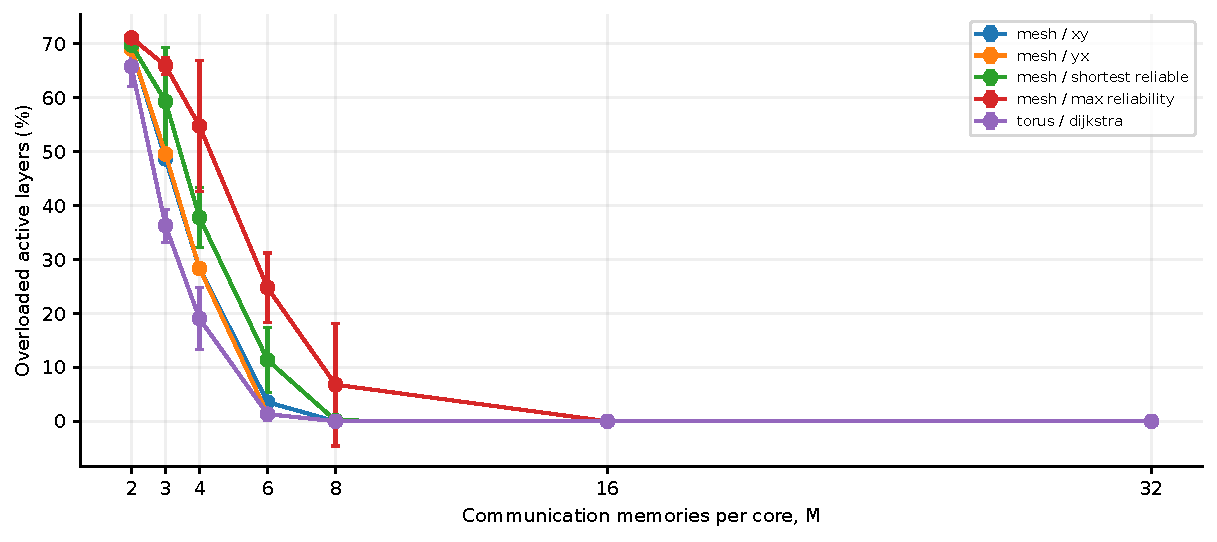
\includegraphics[width=.94\linewidth,height=.34\textheight,keepaspectratio]{figures/summary/congestion_route_overloaded_layer_percent.pdf}\captionof{figure}{Mean and sample SD across three conceptual reliability-seed labels. Identical route aliases are not independent mappings.}\end{center}
\begin{center}{\scriptsize\setlength{\tabcolsep}{3pt}
\begin{tabular}{lrrrrr}
\toprule
M & XY & YX & Short-rel & Max-rel & Torus Dijk. \\
\midrule
2 & $69.027\pm0.000$ & $69.027\pm0.000$ & $69.764\pm1.842$ & $71.091\pm0.255$ & $65.782\pm3.763$ \\
3 & $48.673\pm0.000$ & $49.558\pm0.000$ & $59.292\pm10.051$ & $65.929\pm1.595$ & $36.283\pm3.066$ \\
4 & $28.319\pm0.000$ & $28.319\pm0.000$ & $37.758\pm5.568$ & $54.720\pm12.137$ & $19.027\pm5.752$ \\
6 & $3.540\pm0.000$ & $1.327\pm0.000$ & $11.357\pm6.104$ & $24.779\pm6.427$ & $1.327\pm1.171$ \\
8 & $0.0000\pm0.0000$ & $0.0000\pm0.0000$ & $0.1475\pm0.2555$ & $6.785\pm11.370$ & $0.0000\pm0.0000$ \\
16 & $0.0000\pm0.0000$ & $0.0000\pm0.0000$ & $0.0000\pm0.0000$ & $0.0000\pm0.0000$ & $0.0000\pm0.0000$ \\
32 & $0.0000\pm0.0000$ & $0.0000\pm0.0000$ & $0.0000\pm0.0000$ & $0.0000\pm0.0000$ & $0.0000\pm0.0000$ \\
\bottomrule\end{tabular}}
\captionof{table}{Overloaded active layers (\%) for route counting.}
{\footnotesize\href{https://github.com/sanjeevkrishnaa/Compiler-Driven-ACE/blob/codex/ace-scheduler-correctness/docs/latex/qft96_final/data/congestion_overview.csv}{Exact CSV values and sample counts}}
\end{center}
\clearpage\section*{Route counting: Overloaded core-layers}
\begin{center}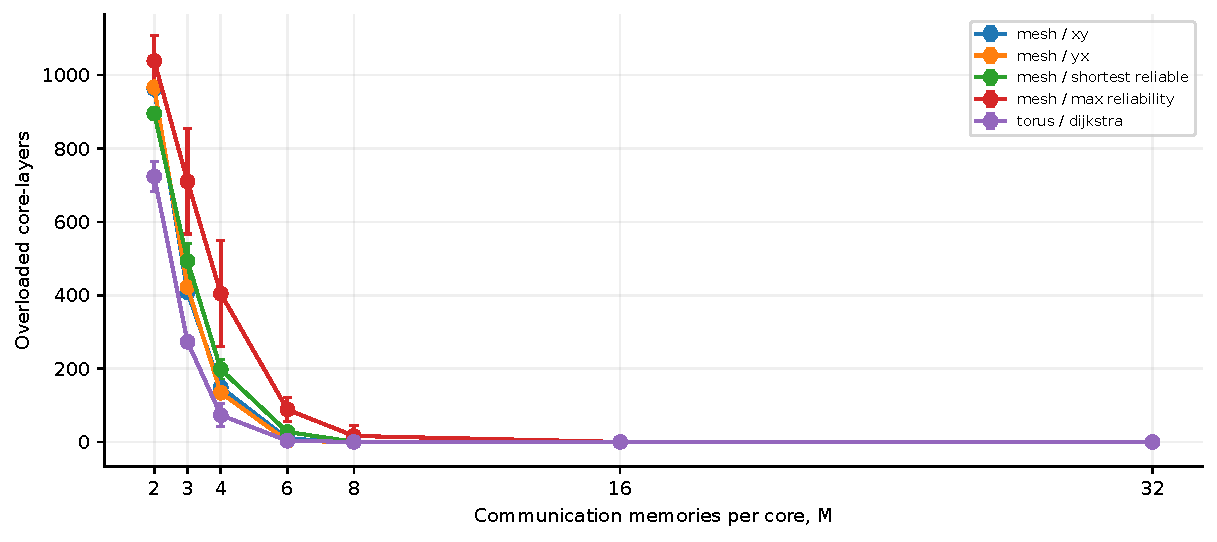
\includegraphics[width=.94\linewidth,height=.34\textheight,keepaspectratio]{figures/summary/congestion_route_overloaded_core_layers.pdf}\captionof{figure}{Mean and sample SD across three conceptual reliability-seed labels. Identical route aliases are not independent mappings.}\end{center}
\begin{center}{\scriptsize\setlength{\tabcolsep}{3pt}
\begin{tabular}{lrrrrr}
\toprule
M & XY & YX & Short-rel & Max-rel & Torus Dijk. \\
\midrule
2 & $962.00\pm0.00$ & $967.00\pm0.00$ & $895.33\pm15.04$ & $1038.67\pm70.49$ & $723.67\pm41.96$ \\
3 & $408.00\pm0.00$ & $422.00\pm0.00$ & $493.33\pm47.35$ & $710.33\pm143.49$ & $273.00\pm4.36$ \\
4 & $149.00\pm0.00$ & $134.00\pm0.00$ & $197.67\pm27.75$ & $404.33\pm144.07$ & $73.000\pm31.048$ \\
6 & $9.000\pm0.000$ & $3.000\pm0.000$ & $27.333\pm13.429$ & $88.333\pm33.292$ & $3.333\pm2.887$ \\
8 & $0.0000\pm0.0000$ & $0.0000\pm0.0000$ & $0.3333\pm0.5774$ & $16.333\pm27.429$ & $0.0000\pm0.0000$ \\
16 & $0.0000\pm0.0000$ & $0.0000\pm0.0000$ & $0.0000\pm0.0000$ & $0.0000\pm0.0000$ & $0.0000\pm0.0000$ \\
32 & $0.0000\pm0.0000$ & $0.0000\pm0.0000$ & $0.0000\pm0.0000$ & $0.0000\pm0.0000$ & $0.0000\pm0.0000$ \\
\bottomrule\end{tabular}}
\captionof{table}{Overloaded core-layers for route counting.}
{\footnotesize\href{https://github.com/sanjeevkrishnaa/Compiler-Driven-ACE/blob/codex/ace-scheduler-correctness/docs/latex/qft96_final/data/congestion_overview.csv}{Exact CSV values and sample counts}}
\end{center}
\clearpage\section*{Route counting: Excess demand}
\begin{center}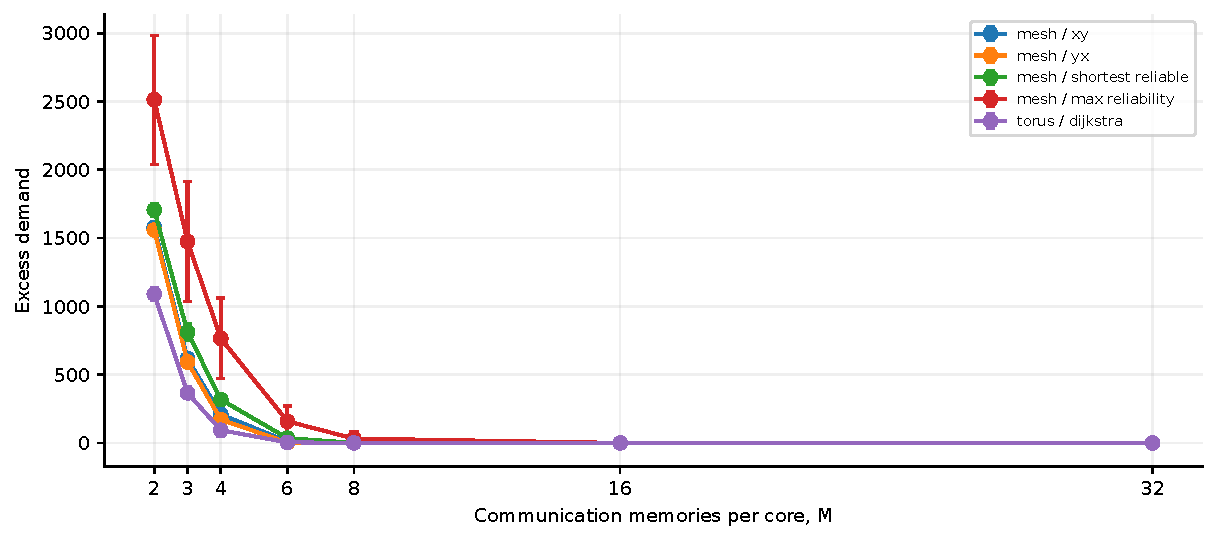
\includegraphics[width=.94\linewidth,height=.34\textheight,keepaspectratio]{figures/summary/congestion_route_excess_demand.pdf}\captionof{figure}{Mean and sample SD across three conceptual reliability-seed labels. Identical route aliases are not independent mappings.}\end{center}
\begin{center}{\scriptsize\setlength{\tabcolsep}{3pt}
\begin{tabular}{lrrrrr}
\toprule
M & XY & YX & Short-rel & Max-rel & Torus Dijk. \\
\midrule
2 & $1579.00\pm0.00$ & $1560.00\pm0.00$ & $1706.33\pm47.65$ & $2514.00\pm472.90$ & $1090.00\pm50.21$ \\
3 & $617.00\pm0.00$ & $593.00\pm0.00$ & $811.00\pm62.22$ & $1475.33\pm438.79$ & $366.33\pm43.39$ \\
4 & $209.00\pm0.00$ & $171.00\pm0.00$ & $317.67\pm17.62$ & $765.00\pm296.14$ & $93.333\pm46.608$ \\
6 & $11.000\pm0.000$ & $3.000\pm0.000$ & $35.000\pm17.349$ & $158.33\pm112.17$ & $4.667\pm4.163$ \\
8 & $0.0000\pm0.0000$ & $0.0000\pm0.0000$ & $0.3333\pm0.5774$ & $32.000\pm54.562$ & $0.0000\pm0.0000$ \\
16 & $0.0000\pm0.0000$ & $0.0000\pm0.0000$ & $0.0000\pm0.0000$ & $0.0000\pm0.0000$ & $0.0000\pm0.0000$ \\
32 & $0.0000\pm0.0000$ & $0.0000\pm0.0000$ & $0.0000\pm0.0000$ & $0.0000\pm0.0000$ & $0.0000\pm0.0000$ \\
\bottomrule\end{tabular}}
\captionof{table}{Excess demand for route counting.}
{\footnotesize\href{https://github.com/sanjeevkrishnaa/Compiler-Driven-ACE/blob/codex/ace-scheduler-correctness/docs/latex/qft96_final/data/congestion_overview.csv}{Exact CSV values and sample counts}}
\end{center}
\clearpage\section*{Hop counting: Overloaded active layers (\%)}
\begin{center}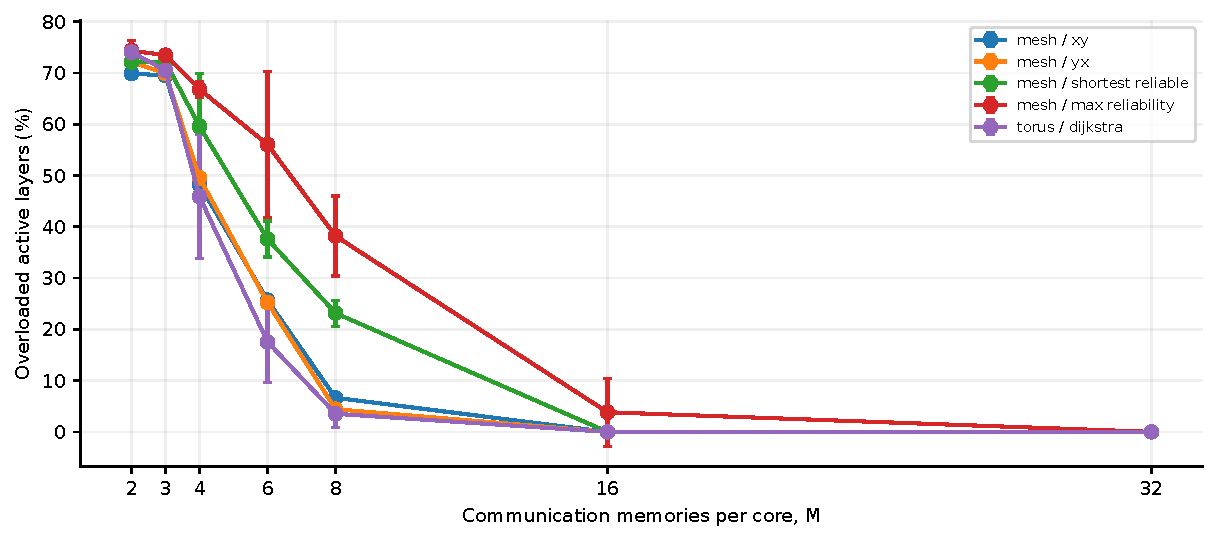
\includegraphics[width=.94\linewidth,height=.34\textheight,keepaspectratio]{figures/summary/congestion_hop_overloaded_layer_percent.pdf}\captionof{figure}{Mean and sample SD across three conceptual reliability-seed labels. Identical route aliases are not independent mappings.}\end{center}
\begin{center}{\scriptsize\setlength{\tabcolsep}{3pt}
\begin{tabular}{lrrrrr}
\toprule
M & XY & YX & Short-rel & Max-rel & Torus Dijk. \\
\midrule
2 & $69.912\pm0.000$ & $72.124\pm0.000$ & $72.124\pm1.533$ & $74.336\pm1.929$ & $74.041\pm0.921$ \\
3 & $69.469\pm0.000$ & $69.912\pm0.000$ & $72.124\pm1.533$ & $73.451\pm0.442$ & $70.501\pm1.114$ \\
4 & $48.230\pm0.000$ & $49.558\pm0.000$ & $59.587\pm10.257$ & $66.814\pm1.595$ & $45.870\pm12.120$ \\
6 & $25.664\pm0.000$ & $25.221\pm0.000$ & $37.611\pm3.512$ & $56.047\pm14.299$ & $17.552\pm7.919$ \\
8 & $6.637\pm0.000$ & $4.425\pm0.000$ & $23.156\pm2.516$ & $38.201\pm7.795$ & $3.540\pm2.763$ \\
16 & $0.0000\pm0.0000$ & $0.0000\pm0.0000$ & $0.0000\pm0.0000$ & $3.835\pm6.642$ & $0.0000\pm0.0000$ \\
32 & $0.0000\pm0.0000$ & $0.0000\pm0.0000$ & $0.0000\pm0.0000$ & $0.0000\pm0.0000$ & $0.0000\pm0.0000$ \\
\bottomrule\end{tabular}}
\captionof{table}{Overloaded active layers (\%) for hop counting.}
{\footnotesize\href{https://github.com/sanjeevkrishnaa/Compiler-Driven-ACE/blob/codex/ace-scheduler-correctness/docs/latex/qft96_final/data/congestion_overview.csv}{Exact CSV values and sample counts}}
\end{center}
\clearpage\section*{Hop counting: Overloaded core-layers}
\begin{center}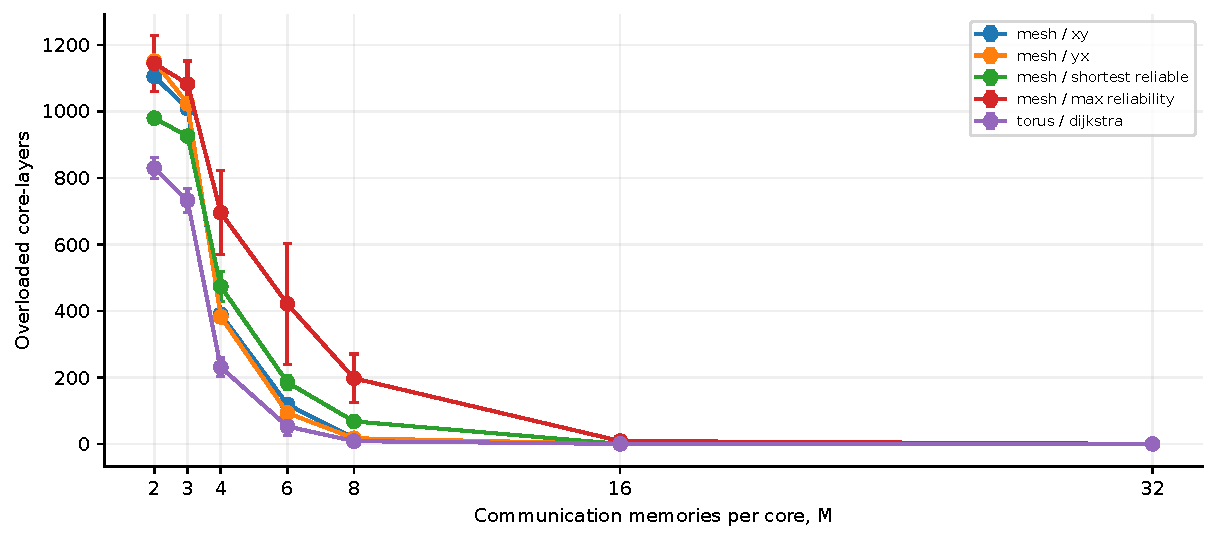
\includegraphics[width=.94\linewidth,height=.34\textheight,keepaspectratio]{figures/summary/congestion_hop_overloaded_core_layers.pdf}\captionof{figure}{Mean and sample SD across three conceptual reliability-seed labels. Identical route aliases are not independent mappings.}\end{center}
\begin{center}{\scriptsize\setlength{\tabcolsep}{3pt}
\begin{tabular}{lrrrrr}
\toprule
M & XY & YX & Short-rel & Max-rel & Torus Dijk. \\
\midrule
2 & $1105.00\pm0.00$ & $1151.00\pm0.00$ & $979.67\pm15.01$ & $1144.33\pm85.15$ & $829.33\pm31.77$ \\
3 & $1008.00\pm0.00$ & $1023.00\pm0.00$ & $925.67\pm10.02$ & $1082.67\pm68.81$ & $731.67\pm36.47$ \\
4 & $390.00\pm0.00$ & $382.00\pm0.00$ & $473.33\pm45.94$ & $695.33\pm126.77$ & $230.33\pm28.01$ \\
6 & $119.00\pm0.00$ & $93.000\pm0.000$ & $185.00\pm21.52$ & $420.67\pm181.48$ & $52.667\pm28.361$ \\
8 & $17.000\pm0.000$ & $17.000\pm0.000$ & $67.667\pm9.238$ & $197.33\pm73.11$ & $8.333\pm6.429$ \\
16 & $0.0000\pm0.0000$ & $0.0000\pm0.0000$ & $0.0000\pm0.0000$ & $8.667\pm15.011$ & $0.0000\pm0.0000$ \\
32 & $0.0000\pm0.0000$ & $0.0000\pm0.0000$ & $0.0000\pm0.0000$ & $0.0000\pm0.0000$ & $0.0000\pm0.0000$ \\
\bottomrule\end{tabular}}
\captionof{table}{Overloaded core-layers for hop counting.}
{\footnotesize\href{https://github.com/sanjeevkrishnaa/Compiler-Driven-ACE/blob/codex/ace-scheduler-correctness/docs/latex/qft96_final/data/congestion_overview.csv}{Exact CSV values and sample counts}}
\end{center}
\clearpage\section*{Hop counting: Excess demand}
\begin{center}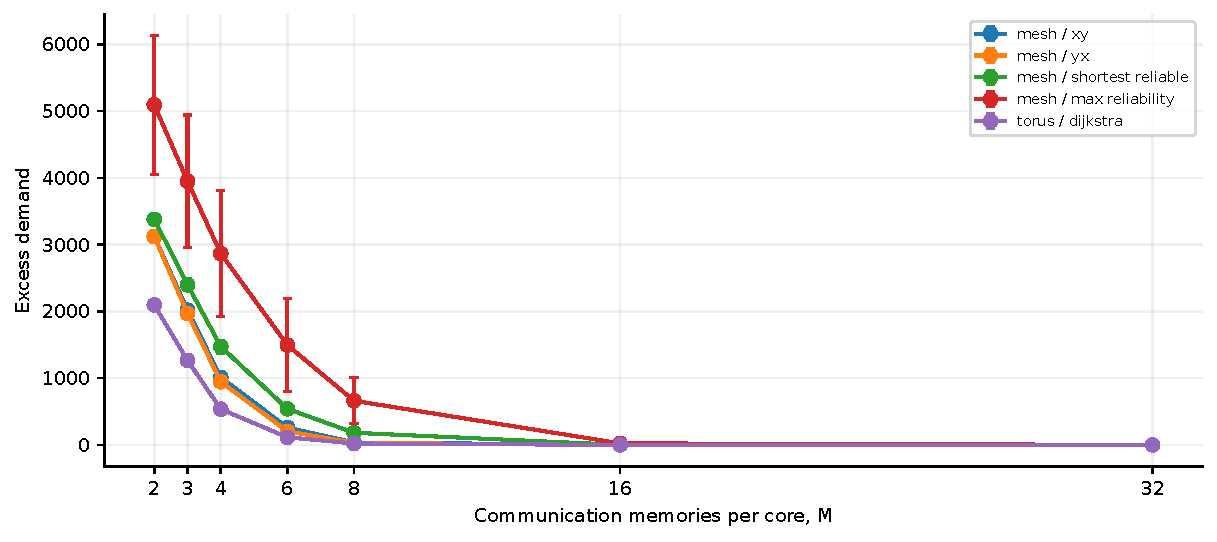
\includegraphics[width=.94\linewidth,height=.34\textheight,keepaspectratio]{figures/summary/congestion_hop_excess_demand.pdf}\captionof{figure}{Mean and sample SD across three conceptual reliability-seed labels. Identical route aliases are not independent mappings.}\end{center}
\begin{center}{\scriptsize\setlength{\tabcolsep}{3pt}
\begin{tabular}{lrrrrr}
\toprule
M & XY & YX & Short-rel & Max-rel & Torus Dijk. \\
\midrule
2 & $3124.00\pm0.00$ & $3120.00\pm0.00$ & $3378.00\pm77.95$ & $5093.33\pm1045.34$ & $2096.33\pm48.79$ \\
3 & $2019.00\pm0.00$ & $1969.00\pm0.00$ & $2398.33\pm89.20$ & $3949.00\pm992.16$ & $1267.00\pm42.23$ \\
4 & $1011.00\pm0.00$ & $946.00\pm0.00$ & $1472.67\pm97.39$ & $2866.33\pm946.75$ & $535.33\pm52.79$ \\
6 & $260.00\pm0.00$ & $203.00\pm0.00$ & $540.33\pm24.21$ & $1495.00\pm691.03$ & $114.00\pm72.19$ \\
8 & $36.000\pm0.000$ & $30.000\pm0.000$ & $181.67\pm49.07$ & $661.33\pm341.95$ & $21.667\pm18.230$ \\
16 & $0.0000\pm0.0000$ & $0.0000\pm0.0000$ & $0.0000\pm0.0000$ & $23.000\pm39.837$ & $0.0000\pm0.0000$ \\
32 & $0.0000\pm0.0000$ & $0.0000\pm0.0000$ & $0.0000\pm0.0000$ & $0.0000\pm0.0000$ & $0.0000\pm0.0000$ \\
\bottomrule\end{tabular}}
\captionof{table}{Excess demand for hop counting.}
{\footnotesize\href{https://github.com/sanjeevkrishnaa/Compiler-Driven-ACE/blob/codex/ace-scheduler-correctness/docs/latex/qft96_final/data/congestion_overview.csv}{Exact CSV values and sample counts}}
\end{center}
\section{Mesh / xy}
\clearpage\subsection*{Mesh xy; M=2; route counting}
\begin{center}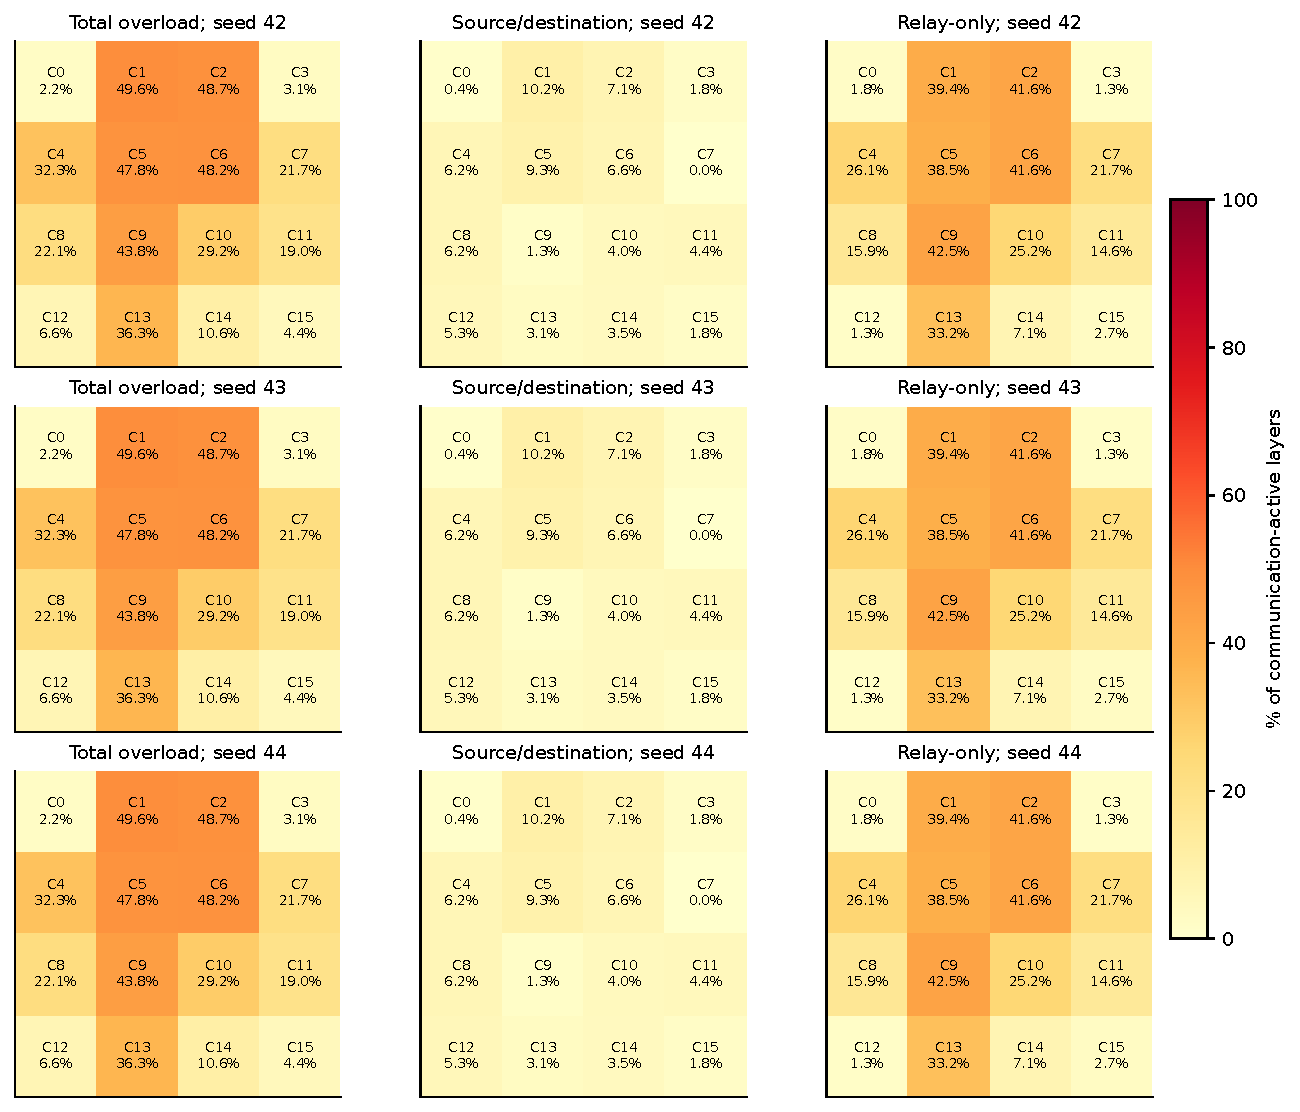
\includegraphics[width=.94\linewidth,height=.48\textheight,keepaspectratio]{figures/atlas/mesh_xy_route_m2.pdf}\captionof{figure}{All three conceptual mapping seeds; common 0--100 percent colour scale.}\end{center}
\begin{center}{\scriptsize\setlength{\tabcolsep}{3pt}
\begin{tabular}{lrrrrrrrrr}
\toprule
Core & 42 Tot & 42 Own & 42 Rel & 43 Tot & 43 Own & 43 Rel & 44 Tot & 44 Own & 44 Rel \\
\midrule
0 & 2.212 & 0.442 & 1.770 & 2.212 & 0.442 & 1.770 & 2.212 & 0.442 & 1.770 \\
1 & 49.558 & 10.177 & 39.381 & 49.558 & 10.177 & 39.381 & 49.558 & 10.177 & 39.381 \\
2 & 48.673 & 7.080 & 41.593 & 48.673 & 7.080 & 41.593 & 48.673 & 7.080 & 41.593 \\
3 & 3.097 & 1.770 & 1.327 & 3.097 & 1.770 & 1.327 & 3.097 & 1.770 & 1.327 \\
4 & 32.301 & 6.195 & 26.106 & 32.301 & 6.195 & 26.106 & 32.301 & 6.195 & 26.106 \\
5 & 47.788 & 9.292 & 38.496 & 47.788 & 9.292 & 38.496 & 47.788 & 9.292 & 38.496 \\
6 & 48.230 & 6.637 & 41.593 & 48.230 & 6.637 & 41.593 & 48.230 & 6.637 & 41.593 \\
7 & 21.681 & 0.000 & 21.681 & 21.681 & 0.000 & 21.681 & 21.681 & 0.000 & 21.681 \\
8 & 22.124 & 6.195 & 15.929 & 22.124 & 6.195 & 15.929 & 22.124 & 6.195 & 15.929 \\
9 & 43.805 & 1.327 & 42.478 & 43.805 & 1.327 & 42.478 & 43.805 & 1.327 & 42.478 \\
10 & 29.204 & 3.982 & 25.221 & 29.204 & 3.982 & 25.221 & 29.204 & 3.982 & 25.221 \\
11 & 19.027 & 4.425 & 14.602 & 19.027 & 4.425 & 14.602 & 19.027 & 4.425 & 14.602 \\
12 & 6.637 & 5.310 & 1.327 & 6.637 & 5.310 & 1.327 & 6.637 & 5.310 & 1.327 \\
13 & 36.283 & 3.097 & 33.186 & 36.283 & 3.097 & 33.186 & 36.283 & 3.097 & 33.186 \\
14 & 10.619 & 3.540 & 7.080 & 10.619 & 3.540 & 7.080 & 10.619 & 3.540 & 7.080 \\
15 & 4.425 & 1.770 & 2.655 & 4.425 & 1.770 & 2.655 & 4.425 & 1.770 & 2.655 \\
\bottomrule\end{tabular}}
\captionof{table}{Exact heatmap percentages, with Tot = Own + Rel. Unrounded values are in the CSV.}
{\footnotesize\href{https://github.com/sanjeevkrishnaa/Compiler-Driven-ACE/blob/codex/ace-scheduler-correctness/docs/latex/qft96_final/data/heatmap_mesh_xy_route_m2.csv}{Exact CSV values and sample counts}}
\end{center}
\clearpage\subsection*{Mesh xy; M=3; route counting}
\begin{center}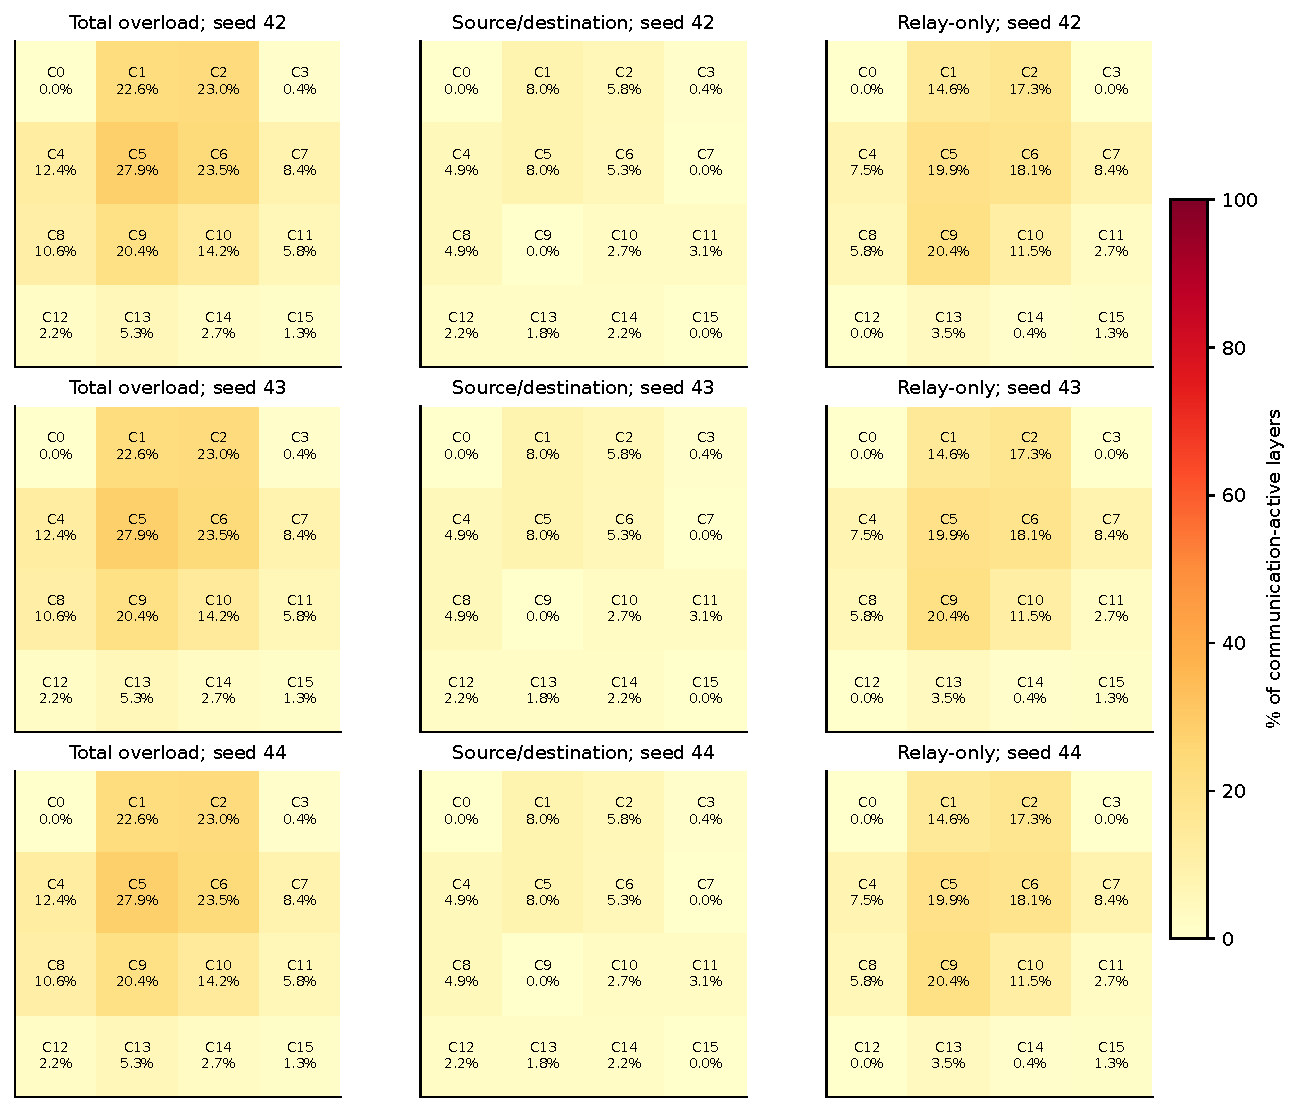
\includegraphics[width=.94\linewidth,height=.48\textheight,keepaspectratio]{figures/atlas/mesh_xy_route_m3.pdf}\captionof{figure}{All three conceptual mapping seeds; common 0--100 percent colour scale.}\end{center}
\begin{center}{\scriptsize\setlength{\tabcolsep}{3pt}
\begin{tabular}{lrrrrrrrrr}
\toprule
Core & 42 Tot & 42 Own & 42 Rel & 43 Tot & 43 Own & 43 Rel & 44 Tot & 44 Own & 44 Rel \\
\midrule
0 & 0.000 & 0.000 & 0.000 & 0.000 & 0.000 & 0.000 & 0.000 & 0.000 & 0.000 \\
1 & 22.566 & 7.965 & 14.602 & 22.566 & 7.965 & 14.602 & 22.566 & 7.965 & 14.602 \\
2 & 23.009 & 5.752 & 17.257 & 23.009 & 5.752 & 17.257 & 23.009 & 5.752 & 17.257 \\
3 & 0.442 & 0.442 & 0.000 & 0.442 & 0.442 & 0.000 & 0.442 & 0.442 & 0.000 \\
4 & 12.389 & 4.867 & 7.522 & 12.389 & 4.867 & 7.522 & 12.389 & 4.867 & 7.522 \\
5 & 27.876 & 7.965 & 19.912 & 27.876 & 7.965 & 19.912 & 27.876 & 7.965 & 19.912 \\
6 & 23.451 & 5.310 & 18.142 & 23.451 & 5.310 & 18.142 & 23.451 & 5.310 & 18.142 \\
7 & 8.407 & 0.000 & 8.407 & 8.407 & 0.000 & 8.407 & 8.407 & 0.000 & 8.407 \\
8 & 10.619 & 4.867 & 5.752 & 10.619 & 4.867 & 5.752 & 10.619 & 4.867 & 5.752 \\
9 & 20.354 & 0.000 & 20.354 & 20.354 & 0.000 & 20.354 & 20.354 & 0.000 & 20.354 \\
10 & 14.159 & 2.655 & 11.504 & 14.159 & 2.655 & 11.504 & 14.159 & 2.655 & 11.504 \\
11 & 5.752 & 3.097 & 2.655 & 5.752 & 3.097 & 2.655 & 5.752 & 3.097 & 2.655 \\
12 & 2.212 & 2.212 & 0.000 & 2.212 & 2.212 & 0.000 & 2.212 & 2.212 & 0.000 \\
13 & 5.310 & 1.770 & 3.540 & 5.310 & 1.770 & 3.540 & 5.310 & 1.770 & 3.540 \\
14 & 2.655 & 2.212 & 0.442 & 2.655 & 2.212 & 0.442 & 2.655 & 2.212 & 0.442 \\
15 & 1.327 & 0.000 & 1.327 & 1.327 & 0.000 & 1.327 & 1.327 & 0.000 & 1.327 \\
\bottomrule\end{tabular}}
\captionof{table}{Exact heatmap percentages, with Tot = Own + Rel. Unrounded values are in the CSV.}
{\footnotesize\href{https://github.com/sanjeevkrishnaa/Compiler-Driven-ACE/blob/codex/ace-scheduler-correctness/docs/latex/qft96_final/data/heatmap_mesh_xy_route_m3.csv}{Exact CSV values and sample counts}}
\end{center}
\clearpage\subsection*{Mesh xy; M=4; route counting}
\begin{center}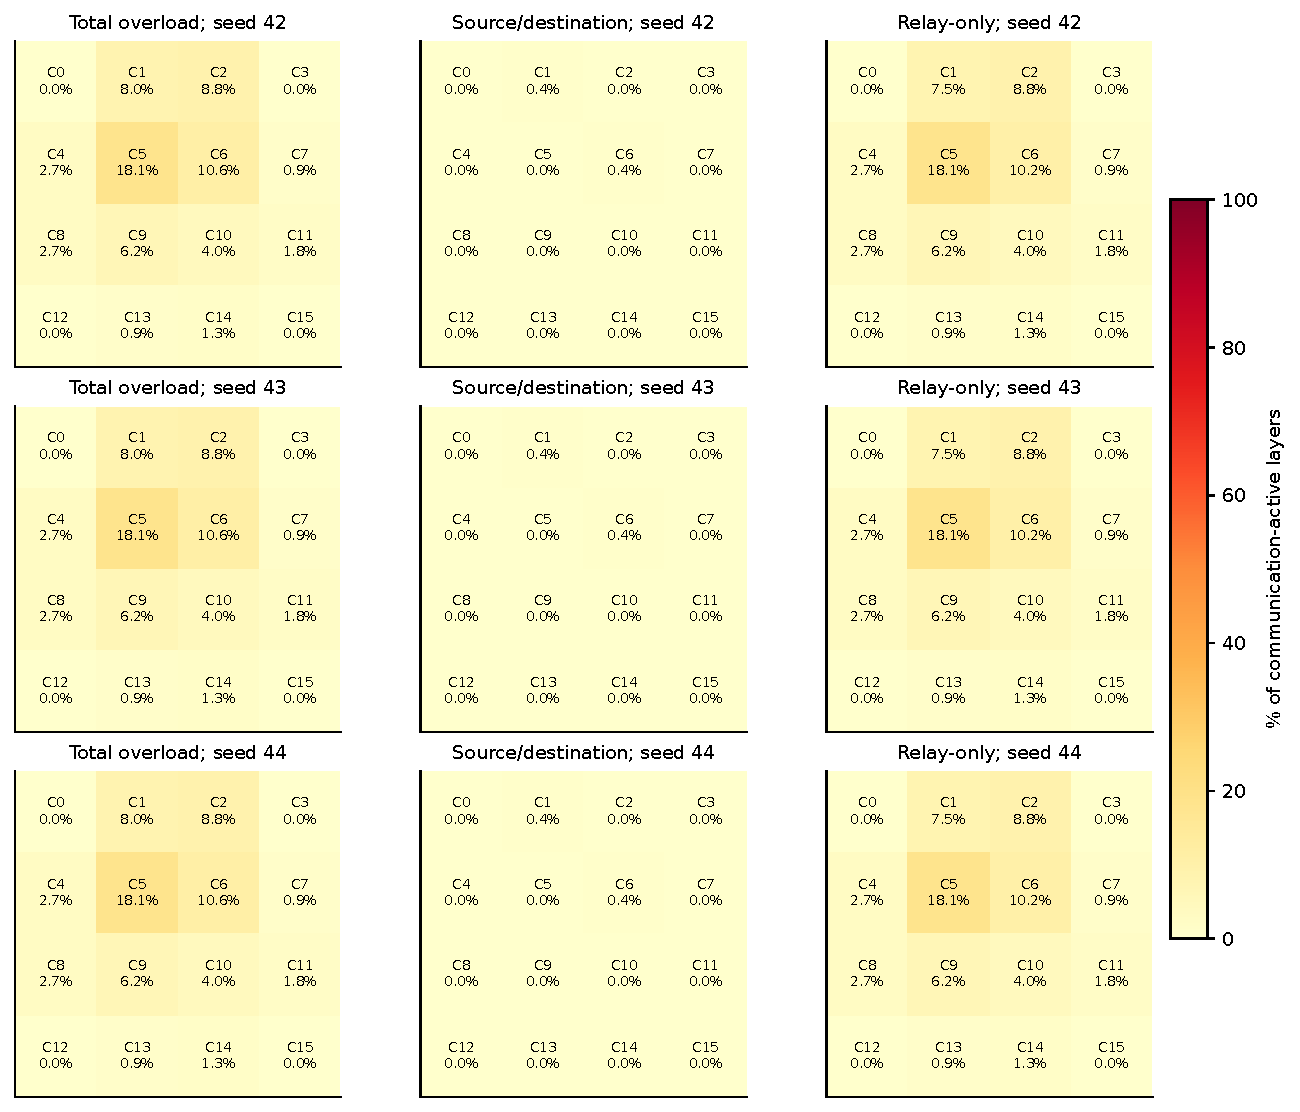
\includegraphics[width=.94\linewidth,height=.48\textheight,keepaspectratio]{figures/atlas/mesh_xy_route_m4.pdf}\captionof{figure}{All three conceptual mapping seeds; common 0--100 percent colour scale.}\end{center}
\begin{center}{\scriptsize\setlength{\tabcolsep}{3pt}
\begin{tabular}{lrrrrrrrrr}
\toprule
Core & 42 Tot & 42 Own & 42 Rel & 43 Tot & 43 Own & 43 Rel & 44 Tot & 44 Own & 44 Rel \\
\midrule
0 & 0.000 & 0.000 & 0.000 & 0.000 & 0.000 & 0.000 & 0.000 & 0.000 & 0.000 \\
1 & 7.965 & 0.442 & 7.522 & 7.965 & 0.442 & 7.522 & 7.965 & 0.442 & 7.522 \\
2 & 8.850 & 0.000 & 8.850 & 8.850 & 0.000 & 8.850 & 8.850 & 0.000 & 8.850 \\
3 & 0.000 & 0.000 & 0.000 & 0.000 & 0.000 & 0.000 & 0.000 & 0.000 & 0.000 \\
4 & 2.655 & 0.000 & 2.655 & 2.655 & 0.000 & 2.655 & 2.655 & 0.000 & 2.655 \\
5 & 18.142 & 0.000 & 18.142 & 18.142 & 0.000 & 18.142 & 18.142 & 0.000 & 18.142 \\
6 & 10.619 & 0.442 & 10.177 & 10.619 & 0.442 & 10.177 & 10.619 & 0.442 & 10.177 \\
7 & 0.885 & 0.000 & 0.885 & 0.885 & 0.000 & 0.885 & 0.885 & 0.000 & 0.885 \\
8 & 2.655 & 0.000 & 2.655 & 2.655 & 0.000 & 2.655 & 2.655 & 0.000 & 2.655 \\
9 & 6.195 & 0.000 & 6.195 & 6.195 & 0.000 & 6.195 & 6.195 & 0.000 & 6.195 \\
10 & 3.982 & 0.000 & 3.982 & 3.982 & 0.000 & 3.982 & 3.982 & 0.000 & 3.982 \\
11 & 1.770 & 0.000 & 1.770 & 1.770 & 0.000 & 1.770 & 1.770 & 0.000 & 1.770 \\
12 & 0.000 & 0.000 & 0.000 & 0.000 & 0.000 & 0.000 & 0.000 & 0.000 & 0.000 \\
13 & 0.885 & 0.000 & 0.885 & 0.885 & 0.000 & 0.885 & 0.885 & 0.000 & 0.885 \\
14 & 1.327 & 0.000 & 1.327 & 1.327 & 0.000 & 1.327 & 1.327 & 0.000 & 1.327 \\
15 & 0.000 & 0.000 & 0.000 & 0.000 & 0.000 & 0.000 & 0.000 & 0.000 & 0.000 \\
\bottomrule\end{tabular}}
\captionof{table}{Exact heatmap percentages, with Tot = Own + Rel. Unrounded values are in the CSV.}
{\footnotesize\href{https://github.com/sanjeevkrishnaa/Compiler-Driven-ACE/blob/codex/ace-scheduler-correctness/docs/latex/qft96_final/data/heatmap_mesh_xy_route_m4.csv}{Exact CSV values and sample counts}}
\end{center}
\clearpage\subsection*{Mesh xy; M=6; route counting}
\begin{center}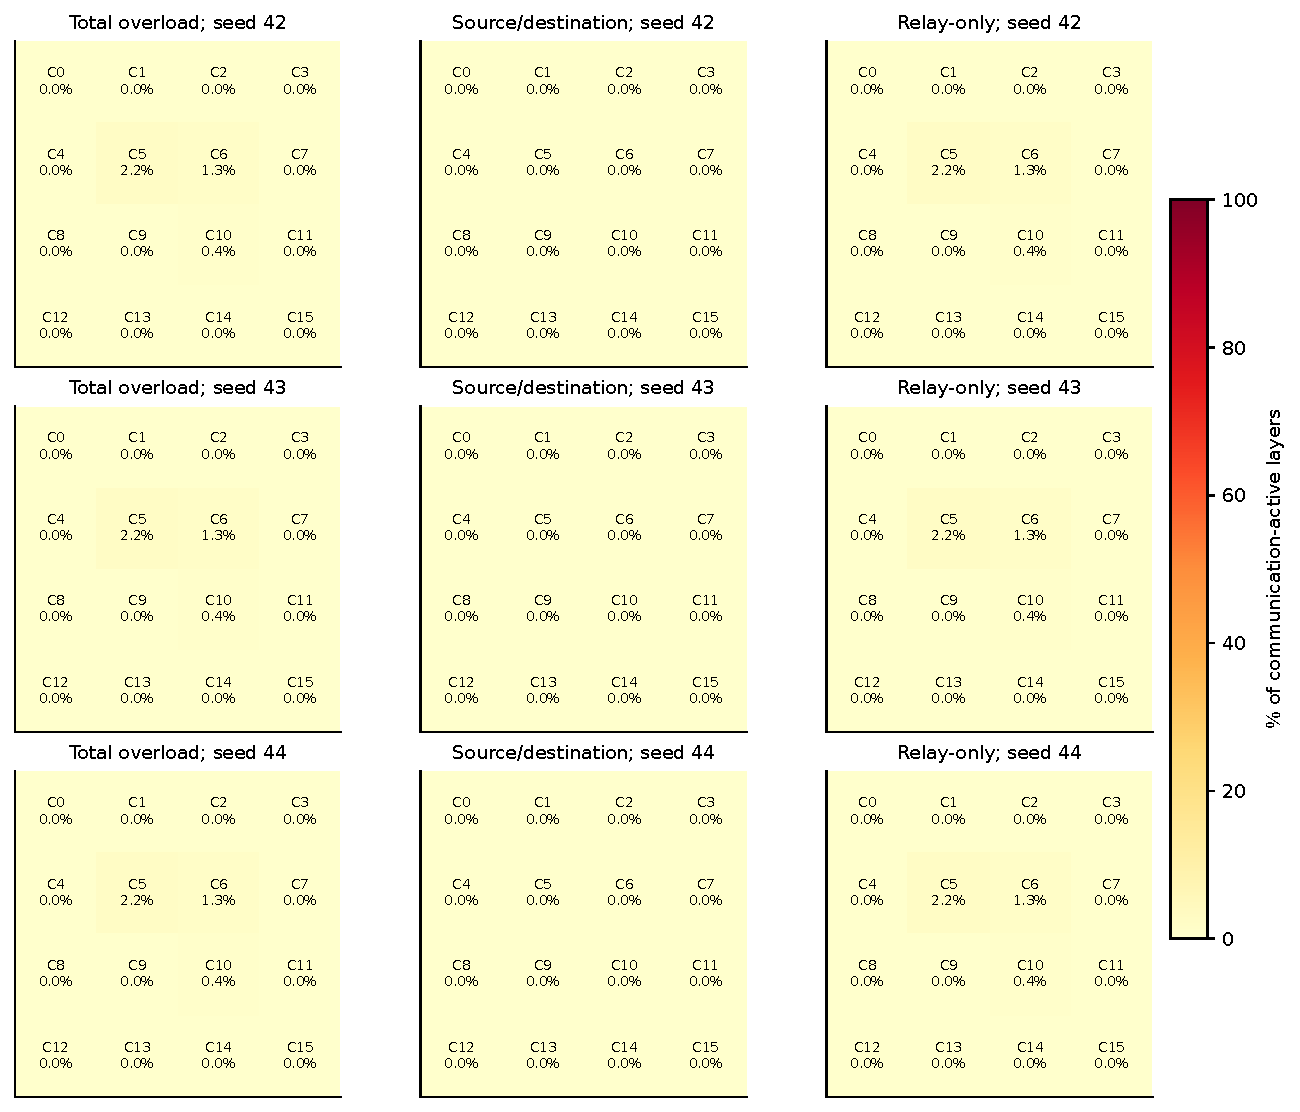
\includegraphics[width=.94\linewidth,height=.48\textheight,keepaspectratio]{figures/atlas/mesh_xy_route_m6.pdf}\captionof{figure}{All three conceptual mapping seeds; common 0--100 percent colour scale.}\end{center}
\begin{center}{\scriptsize\setlength{\tabcolsep}{3pt}
\begin{tabular}{lrrrrrrrrr}
\toprule
Core & 42 Tot & 42 Own & 42 Rel & 43 Tot & 43 Own & 43 Rel & 44 Tot & 44 Own & 44 Rel \\
\midrule
0 & 0.000 & 0.000 & 0.000 & 0.000 & 0.000 & 0.000 & 0.000 & 0.000 & 0.000 \\
1 & 0.000 & 0.000 & 0.000 & 0.000 & 0.000 & 0.000 & 0.000 & 0.000 & 0.000 \\
2 & 0.000 & 0.000 & 0.000 & 0.000 & 0.000 & 0.000 & 0.000 & 0.000 & 0.000 \\
3 & 0.000 & 0.000 & 0.000 & 0.000 & 0.000 & 0.000 & 0.000 & 0.000 & 0.000 \\
4 & 0.000 & 0.000 & 0.000 & 0.000 & 0.000 & 0.000 & 0.000 & 0.000 & 0.000 \\
5 & 2.212 & 0.000 & 2.212 & 2.212 & 0.000 & 2.212 & 2.212 & 0.000 & 2.212 \\
6 & 1.327 & 0.000 & 1.327 & 1.327 & 0.000 & 1.327 & 1.327 & 0.000 & 1.327 \\
7 & 0.000 & 0.000 & 0.000 & 0.000 & 0.000 & 0.000 & 0.000 & 0.000 & 0.000 \\
8 & 0.000 & 0.000 & 0.000 & 0.000 & 0.000 & 0.000 & 0.000 & 0.000 & 0.000 \\
9 & 0.000 & 0.000 & 0.000 & 0.000 & 0.000 & 0.000 & 0.000 & 0.000 & 0.000 \\
10 & 0.442 & 0.000 & 0.442 & 0.442 & 0.000 & 0.442 & 0.442 & 0.000 & 0.442 \\
11 & 0.000 & 0.000 & 0.000 & 0.000 & 0.000 & 0.000 & 0.000 & 0.000 & 0.000 \\
12 & 0.000 & 0.000 & 0.000 & 0.000 & 0.000 & 0.000 & 0.000 & 0.000 & 0.000 \\
13 & 0.000 & 0.000 & 0.000 & 0.000 & 0.000 & 0.000 & 0.000 & 0.000 & 0.000 \\
14 & 0.000 & 0.000 & 0.000 & 0.000 & 0.000 & 0.000 & 0.000 & 0.000 & 0.000 \\
15 & 0.000 & 0.000 & 0.000 & 0.000 & 0.000 & 0.000 & 0.000 & 0.000 & 0.000 \\
\bottomrule\end{tabular}}
\captionof{table}{Exact heatmap percentages, with Tot = Own + Rel. Unrounded values are in the CSV.}
{\footnotesize\href{https://github.com/sanjeevkrishnaa/Compiler-Driven-ACE/blob/codex/ace-scheduler-correctness/docs/latex/qft96_final/data/heatmap_mesh_xy_route_m6.csv}{Exact CSV values and sample counts}}
\end{center}
\clearpage\subsection*{Mesh xy; M=8; route counting}
\begin{center}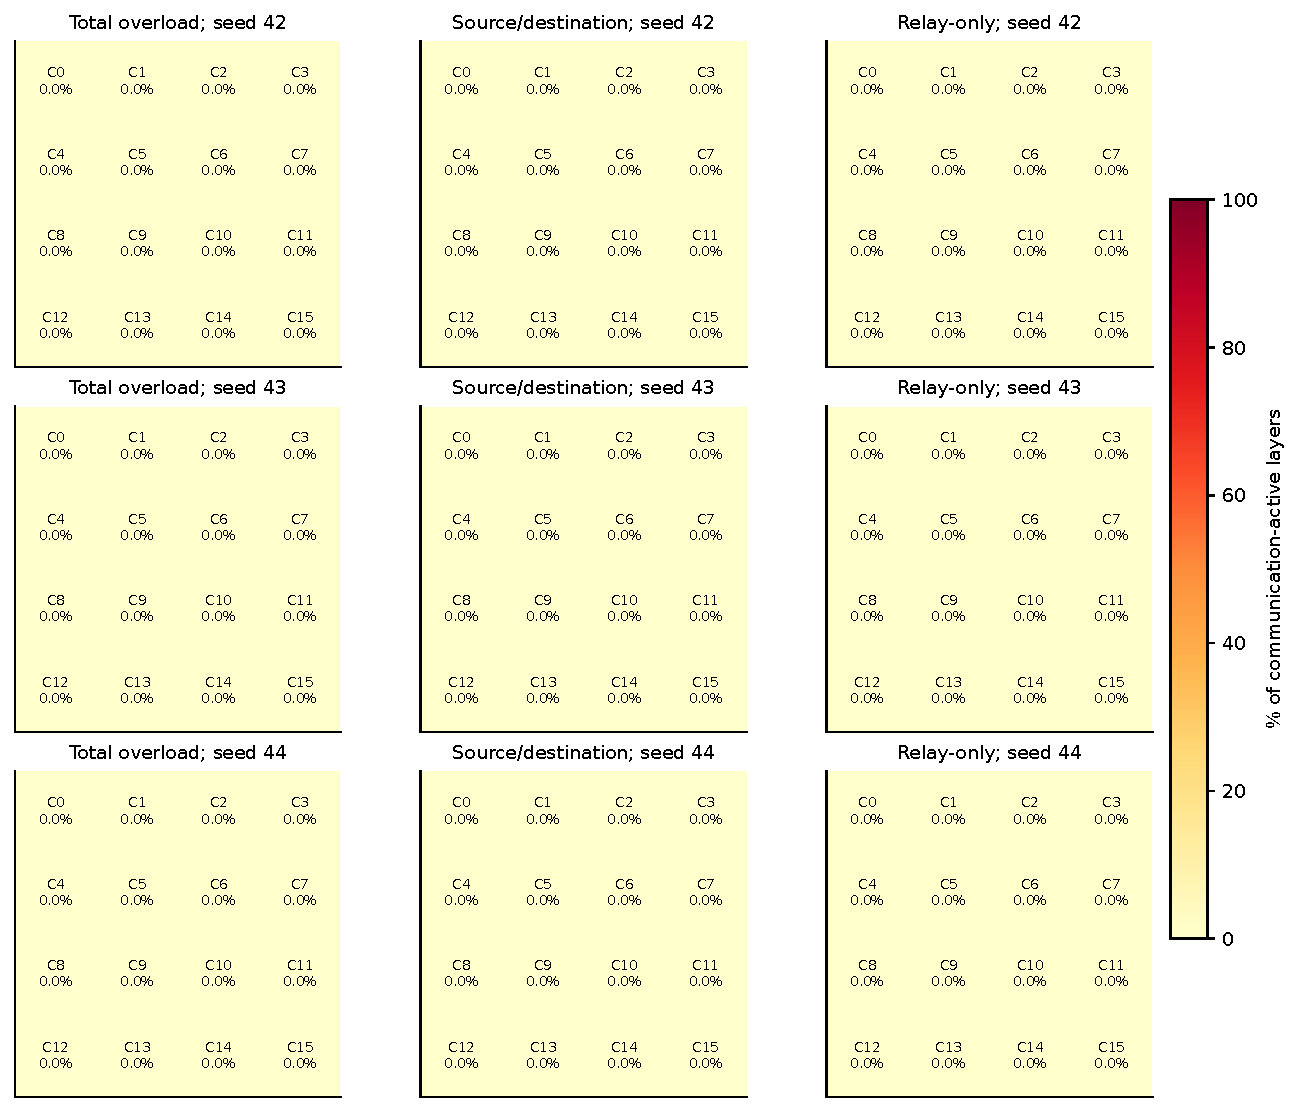
\includegraphics[width=.94\linewidth,height=.48\textheight,keepaspectratio]{figures/atlas/mesh_xy_route_m8.pdf}\captionof{figure}{All three conceptual mapping seeds; common 0--100 percent colour scale.}\end{center}
\begin{center}{\scriptsize\setlength{\tabcolsep}{3pt}
\begin{tabular}{lrrrrrrrrr}
\toprule
Core & 42 Tot & 42 Own & 42 Rel & 43 Tot & 43 Own & 43 Rel & 44 Tot & 44 Own & 44 Rel \\
\midrule
0 & 0.000 & 0.000 & 0.000 & 0.000 & 0.000 & 0.000 & 0.000 & 0.000 & 0.000 \\
1 & 0.000 & 0.000 & 0.000 & 0.000 & 0.000 & 0.000 & 0.000 & 0.000 & 0.000 \\
2 & 0.000 & 0.000 & 0.000 & 0.000 & 0.000 & 0.000 & 0.000 & 0.000 & 0.000 \\
3 & 0.000 & 0.000 & 0.000 & 0.000 & 0.000 & 0.000 & 0.000 & 0.000 & 0.000 \\
4 & 0.000 & 0.000 & 0.000 & 0.000 & 0.000 & 0.000 & 0.000 & 0.000 & 0.000 \\
5 & 0.000 & 0.000 & 0.000 & 0.000 & 0.000 & 0.000 & 0.000 & 0.000 & 0.000 \\
6 & 0.000 & 0.000 & 0.000 & 0.000 & 0.000 & 0.000 & 0.000 & 0.000 & 0.000 \\
7 & 0.000 & 0.000 & 0.000 & 0.000 & 0.000 & 0.000 & 0.000 & 0.000 & 0.000 \\
8 & 0.000 & 0.000 & 0.000 & 0.000 & 0.000 & 0.000 & 0.000 & 0.000 & 0.000 \\
9 & 0.000 & 0.000 & 0.000 & 0.000 & 0.000 & 0.000 & 0.000 & 0.000 & 0.000 \\
10 & 0.000 & 0.000 & 0.000 & 0.000 & 0.000 & 0.000 & 0.000 & 0.000 & 0.000 \\
11 & 0.000 & 0.000 & 0.000 & 0.000 & 0.000 & 0.000 & 0.000 & 0.000 & 0.000 \\
12 & 0.000 & 0.000 & 0.000 & 0.000 & 0.000 & 0.000 & 0.000 & 0.000 & 0.000 \\
13 & 0.000 & 0.000 & 0.000 & 0.000 & 0.000 & 0.000 & 0.000 & 0.000 & 0.000 \\
14 & 0.000 & 0.000 & 0.000 & 0.000 & 0.000 & 0.000 & 0.000 & 0.000 & 0.000 \\
15 & 0.000 & 0.000 & 0.000 & 0.000 & 0.000 & 0.000 & 0.000 & 0.000 & 0.000 \\
\bottomrule\end{tabular}}
\captionof{table}{Exact heatmap percentages, with Tot = Own + Rel. Unrounded values are in the CSV.}
{\footnotesize\href{https://github.com/sanjeevkrishnaa/Compiler-Driven-ACE/blob/codex/ace-scheduler-correctness/docs/latex/qft96_final/data/heatmap_mesh_xy_route_m8.csv}{Exact CSV values and sample counts}}
\end{center}
\clearpage\subsection*{Mesh xy; M=16; route counting}
\begin{center}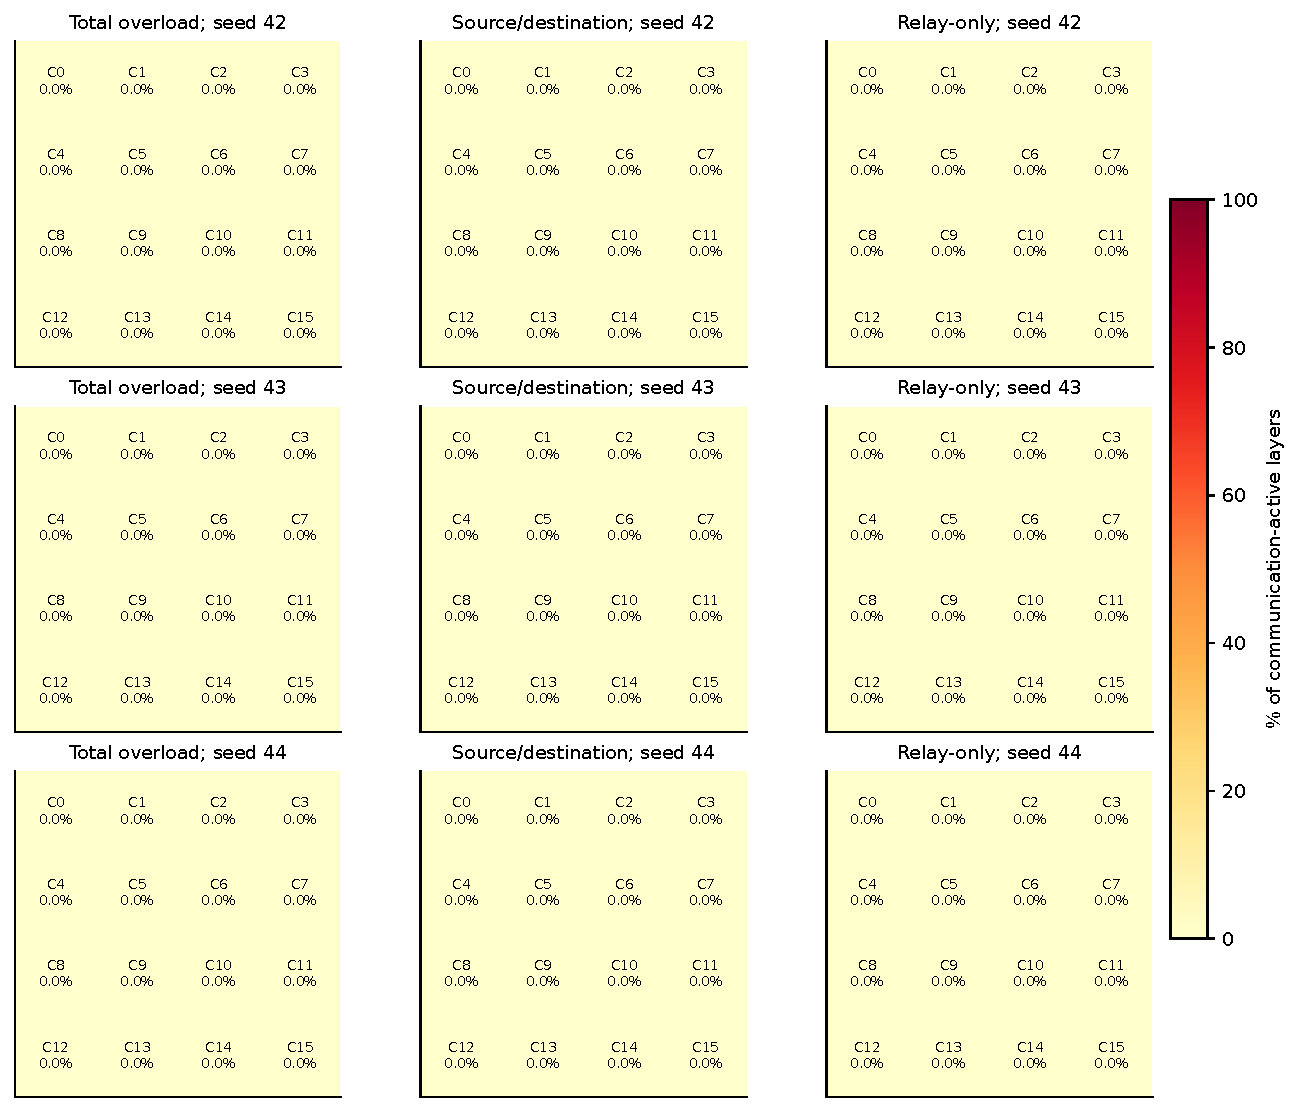
\includegraphics[width=.94\linewidth,height=.48\textheight,keepaspectratio]{figures/atlas/mesh_xy_route_m16.pdf}\captionof{figure}{All three conceptual mapping seeds; common 0--100 percent colour scale.}\end{center}
\begin{center}{\scriptsize\setlength{\tabcolsep}{3pt}
\begin{tabular}{lrrrrrrrrr}
\toprule
Core & 42 Tot & 42 Own & 42 Rel & 43 Tot & 43 Own & 43 Rel & 44 Tot & 44 Own & 44 Rel \\
\midrule
0 & 0.000 & 0.000 & 0.000 & 0.000 & 0.000 & 0.000 & 0.000 & 0.000 & 0.000 \\
1 & 0.000 & 0.000 & 0.000 & 0.000 & 0.000 & 0.000 & 0.000 & 0.000 & 0.000 \\
2 & 0.000 & 0.000 & 0.000 & 0.000 & 0.000 & 0.000 & 0.000 & 0.000 & 0.000 \\
3 & 0.000 & 0.000 & 0.000 & 0.000 & 0.000 & 0.000 & 0.000 & 0.000 & 0.000 \\
4 & 0.000 & 0.000 & 0.000 & 0.000 & 0.000 & 0.000 & 0.000 & 0.000 & 0.000 \\
5 & 0.000 & 0.000 & 0.000 & 0.000 & 0.000 & 0.000 & 0.000 & 0.000 & 0.000 \\
6 & 0.000 & 0.000 & 0.000 & 0.000 & 0.000 & 0.000 & 0.000 & 0.000 & 0.000 \\
7 & 0.000 & 0.000 & 0.000 & 0.000 & 0.000 & 0.000 & 0.000 & 0.000 & 0.000 \\
8 & 0.000 & 0.000 & 0.000 & 0.000 & 0.000 & 0.000 & 0.000 & 0.000 & 0.000 \\
9 & 0.000 & 0.000 & 0.000 & 0.000 & 0.000 & 0.000 & 0.000 & 0.000 & 0.000 \\
10 & 0.000 & 0.000 & 0.000 & 0.000 & 0.000 & 0.000 & 0.000 & 0.000 & 0.000 \\
11 & 0.000 & 0.000 & 0.000 & 0.000 & 0.000 & 0.000 & 0.000 & 0.000 & 0.000 \\
12 & 0.000 & 0.000 & 0.000 & 0.000 & 0.000 & 0.000 & 0.000 & 0.000 & 0.000 \\
13 & 0.000 & 0.000 & 0.000 & 0.000 & 0.000 & 0.000 & 0.000 & 0.000 & 0.000 \\
14 & 0.000 & 0.000 & 0.000 & 0.000 & 0.000 & 0.000 & 0.000 & 0.000 & 0.000 \\
15 & 0.000 & 0.000 & 0.000 & 0.000 & 0.000 & 0.000 & 0.000 & 0.000 & 0.000 \\
\bottomrule\end{tabular}}
\captionof{table}{Exact heatmap percentages, with Tot = Own + Rel. Unrounded values are in the CSV.}
{\footnotesize\href{https://github.com/sanjeevkrishnaa/Compiler-Driven-ACE/blob/codex/ace-scheduler-correctness/docs/latex/qft96_final/data/heatmap_mesh_xy_route_m16.csv}{Exact CSV values and sample counts}}
\end{center}
\clearpage\subsection*{Mesh xy; M=32; route counting}
\begin{center}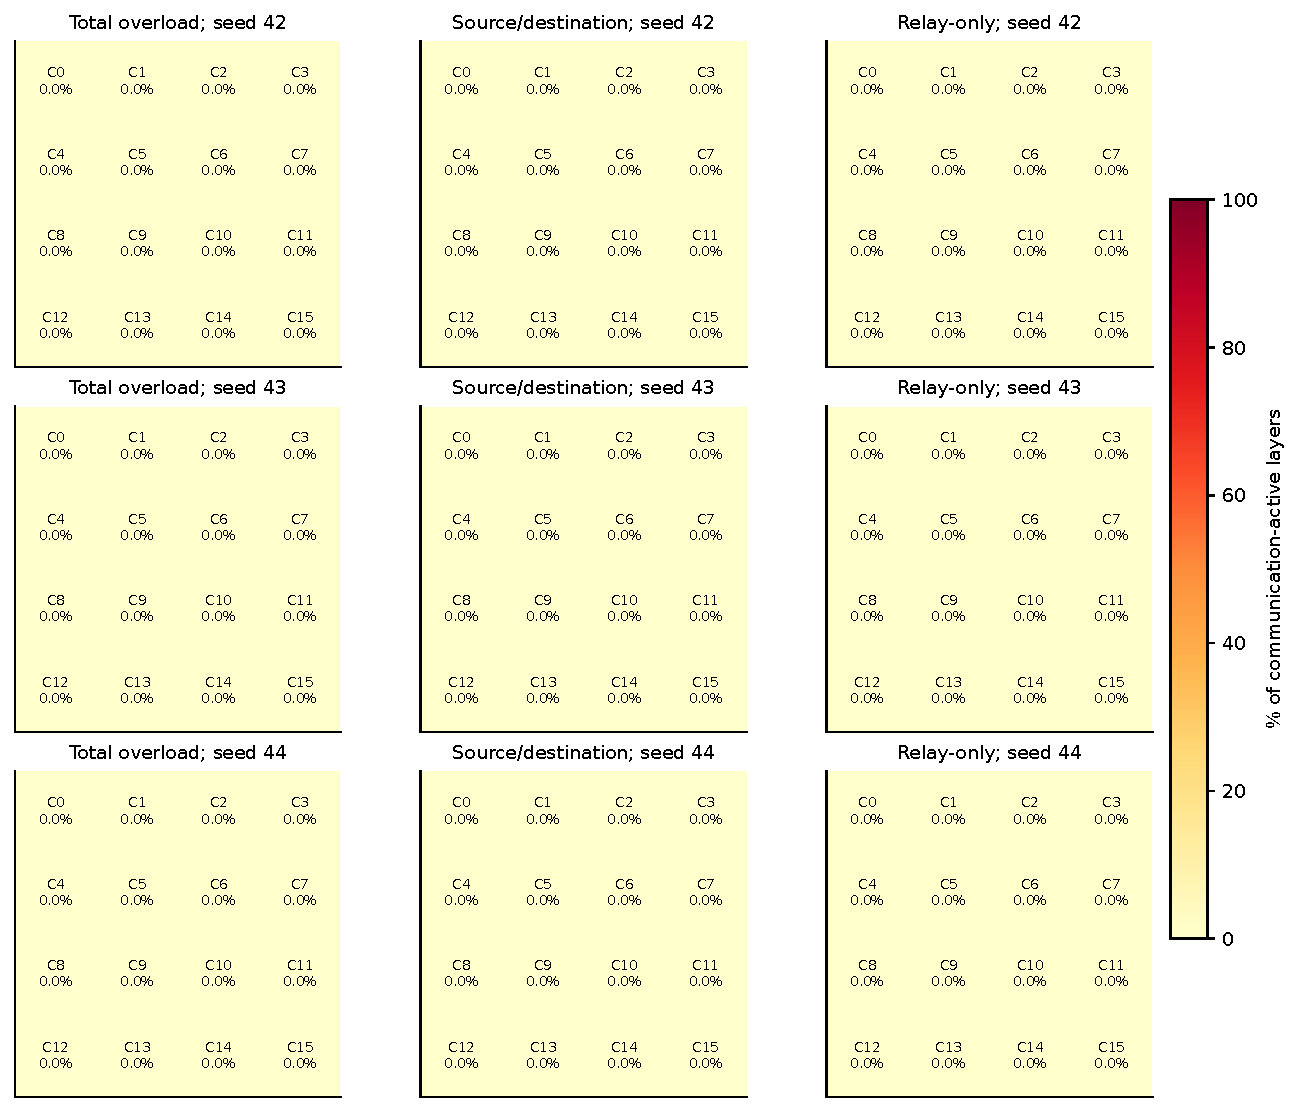
\includegraphics[width=.94\linewidth,height=.48\textheight,keepaspectratio]{figures/atlas/mesh_xy_route_m32.pdf}\captionof{figure}{All three conceptual mapping seeds; common 0--100 percent colour scale.}\end{center}
\begin{center}{\scriptsize\setlength{\tabcolsep}{3pt}
\begin{tabular}{lrrrrrrrrr}
\toprule
Core & 42 Tot & 42 Own & 42 Rel & 43 Tot & 43 Own & 43 Rel & 44 Tot & 44 Own & 44 Rel \\
\midrule
0 & 0.000 & 0.000 & 0.000 & 0.000 & 0.000 & 0.000 & 0.000 & 0.000 & 0.000 \\
1 & 0.000 & 0.000 & 0.000 & 0.000 & 0.000 & 0.000 & 0.000 & 0.000 & 0.000 \\
2 & 0.000 & 0.000 & 0.000 & 0.000 & 0.000 & 0.000 & 0.000 & 0.000 & 0.000 \\
3 & 0.000 & 0.000 & 0.000 & 0.000 & 0.000 & 0.000 & 0.000 & 0.000 & 0.000 \\
4 & 0.000 & 0.000 & 0.000 & 0.000 & 0.000 & 0.000 & 0.000 & 0.000 & 0.000 \\
5 & 0.000 & 0.000 & 0.000 & 0.000 & 0.000 & 0.000 & 0.000 & 0.000 & 0.000 \\
6 & 0.000 & 0.000 & 0.000 & 0.000 & 0.000 & 0.000 & 0.000 & 0.000 & 0.000 \\
7 & 0.000 & 0.000 & 0.000 & 0.000 & 0.000 & 0.000 & 0.000 & 0.000 & 0.000 \\
8 & 0.000 & 0.000 & 0.000 & 0.000 & 0.000 & 0.000 & 0.000 & 0.000 & 0.000 \\
9 & 0.000 & 0.000 & 0.000 & 0.000 & 0.000 & 0.000 & 0.000 & 0.000 & 0.000 \\
10 & 0.000 & 0.000 & 0.000 & 0.000 & 0.000 & 0.000 & 0.000 & 0.000 & 0.000 \\
11 & 0.000 & 0.000 & 0.000 & 0.000 & 0.000 & 0.000 & 0.000 & 0.000 & 0.000 \\
12 & 0.000 & 0.000 & 0.000 & 0.000 & 0.000 & 0.000 & 0.000 & 0.000 & 0.000 \\
13 & 0.000 & 0.000 & 0.000 & 0.000 & 0.000 & 0.000 & 0.000 & 0.000 & 0.000 \\
14 & 0.000 & 0.000 & 0.000 & 0.000 & 0.000 & 0.000 & 0.000 & 0.000 & 0.000 \\
15 & 0.000 & 0.000 & 0.000 & 0.000 & 0.000 & 0.000 & 0.000 & 0.000 & 0.000 \\
\bottomrule\end{tabular}}
\captionof{table}{Exact heatmap percentages, with Tot = Own + Rel. Unrounded values are in the CSV.}
{\footnotesize\href{https://github.com/sanjeevkrishnaa/Compiler-Driven-ACE/blob/codex/ace-scheduler-correctness/docs/latex/qft96_final/data/heatmap_mesh_xy_route_m32.csv}{Exact CSV values and sample counts}}
\end{center}
\clearpage\subsection*{Mesh xy; M=2; hop counting}
\begin{center}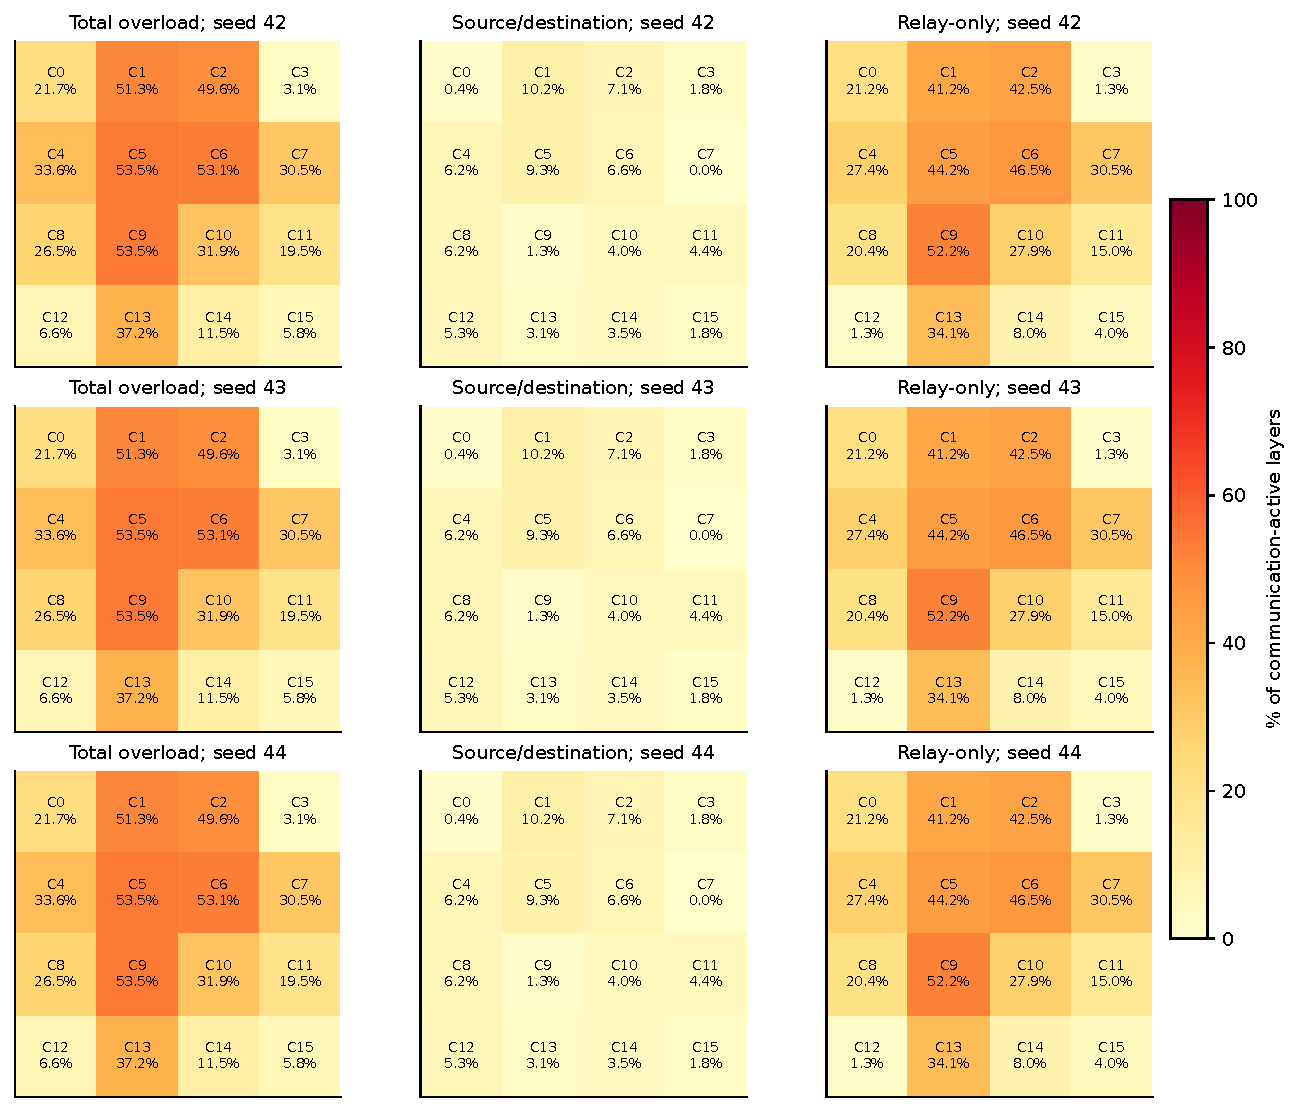
\includegraphics[width=.94\linewidth,height=.48\textheight,keepaspectratio]{figures/atlas/mesh_xy_hop_m2.pdf}\captionof{figure}{All three conceptual mapping seeds; common 0--100 percent colour scale.}\end{center}
\begin{center}{\scriptsize\setlength{\tabcolsep}{3pt}
\begin{tabular}{lrrrrrrrrr}
\toprule
Core & 42 Tot & 42 Own & 42 Rel & 43 Tot & 43 Own & 43 Rel & 44 Tot & 44 Own & 44 Rel \\
\midrule
0 & 21.681 & 0.442 & 21.239 & 21.681 & 0.442 & 21.239 & 21.681 & 0.442 & 21.239 \\
1 & 51.327 & 10.177 & 41.150 & 51.327 & 10.177 & 41.150 & 51.327 & 10.177 & 41.150 \\
2 & 49.558 & 7.080 & 42.478 & 49.558 & 7.080 & 42.478 & 49.558 & 7.080 & 42.478 \\
3 & 3.097 & 1.770 & 1.327 & 3.097 & 1.770 & 1.327 & 3.097 & 1.770 & 1.327 \\
4 & 33.628 & 6.195 & 27.434 & 33.628 & 6.195 & 27.434 & 33.628 & 6.195 & 27.434 \\
5 & 53.540 & 9.292 & 44.248 & 53.540 & 9.292 & 44.248 & 53.540 & 9.292 & 44.248 \\
6 & 53.097 & 6.637 & 46.460 & 53.097 & 6.637 & 46.460 & 53.097 & 6.637 & 46.460 \\
7 & 30.531 & 0.000 & 30.531 & 30.531 & 0.000 & 30.531 & 30.531 & 0.000 & 30.531 \\
8 & 26.549 & 6.195 & 20.354 & 26.549 & 6.195 & 20.354 & 26.549 & 6.195 & 20.354 \\
9 & 53.540 & 1.327 & 52.212 & 53.540 & 1.327 & 52.212 & 53.540 & 1.327 & 52.212 \\
10 & 31.858 & 3.982 & 27.876 & 31.858 & 3.982 & 27.876 & 31.858 & 3.982 & 27.876 \\
11 & 19.469 & 4.425 & 15.044 & 19.469 & 4.425 & 15.044 & 19.469 & 4.425 & 15.044 \\
12 & 6.637 & 5.310 & 1.327 & 6.637 & 5.310 & 1.327 & 6.637 & 5.310 & 1.327 \\
13 & 37.168 & 3.097 & 34.071 & 37.168 & 3.097 & 34.071 & 37.168 & 3.097 & 34.071 \\
14 & 11.504 & 3.540 & 7.965 & 11.504 & 3.540 & 7.965 & 11.504 & 3.540 & 7.965 \\
15 & 5.752 & 1.770 & 3.982 & 5.752 & 1.770 & 3.982 & 5.752 & 1.770 & 3.982 \\
\bottomrule\end{tabular}}
\captionof{table}{Exact heatmap percentages, with Tot = Own + Rel. Unrounded values are in the CSV.}
{\footnotesize\href{https://github.com/sanjeevkrishnaa/Compiler-Driven-ACE/blob/codex/ace-scheduler-correctness/docs/latex/qft96_final/data/heatmap_mesh_xy_hop_m2.csv}{Exact CSV values and sample counts}}
\end{center}
\clearpage\subsection*{Mesh xy; M=3; hop counting}
\begin{center}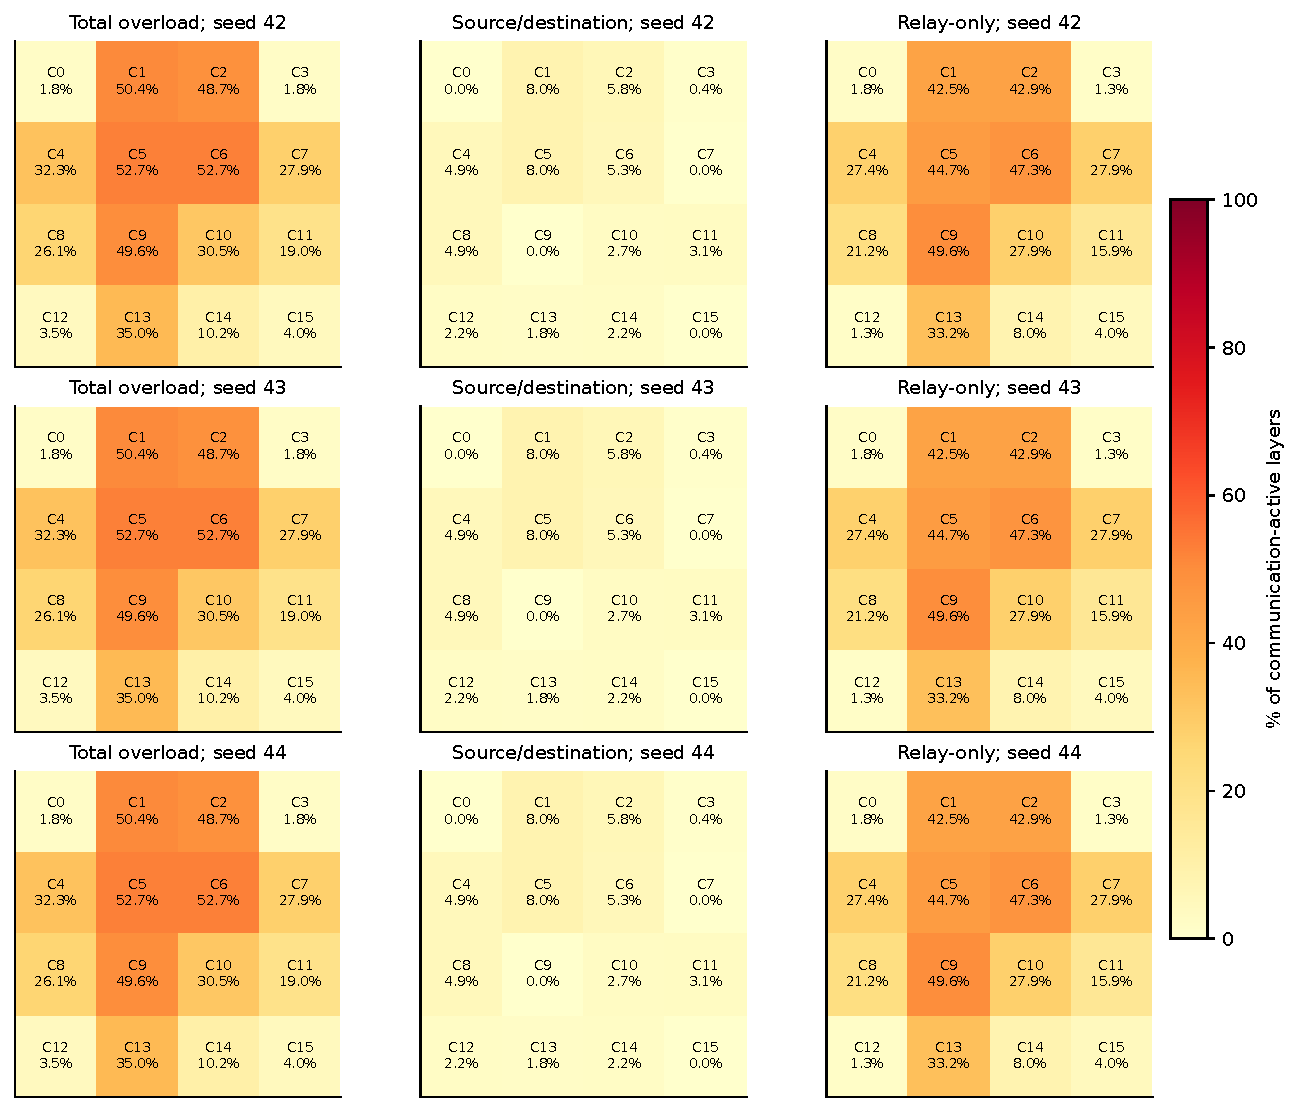
\includegraphics[width=.94\linewidth,height=.48\textheight,keepaspectratio]{figures/atlas/mesh_xy_hop_m3.pdf}\captionof{figure}{All three conceptual mapping seeds; common 0--100 percent colour scale.}\end{center}
\begin{center}{\scriptsize\setlength{\tabcolsep}{3pt}
\begin{tabular}{lrrrrrrrrr}
\toprule
Core & 42 Tot & 42 Own & 42 Rel & 43 Tot & 43 Own & 43 Rel & 44 Tot & 44 Own & 44 Rel \\
\midrule
0 & 1.770 & 0.000 & 1.770 & 1.770 & 0.000 & 1.770 & 1.770 & 0.000 & 1.770 \\
1 & 50.442 & 7.965 & 42.478 & 50.442 & 7.965 & 42.478 & 50.442 & 7.965 & 42.478 \\
2 & 48.673 & 5.752 & 42.920 & 48.673 & 5.752 & 42.920 & 48.673 & 5.752 & 42.920 \\
3 & 1.770 & 0.442 & 1.327 & 1.770 & 0.442 & 1.327 & 1.770 & 0.442 & 1.327 \\
4 & 32.301 & 4.867 & 27.434 & 32.301 & 4.867 & 27.434 & 32.301 & 4.867 & 27.434 \\
5 & 52.655 & 7.965 & 44.690 & 52.655 & 7.965 & 44.690 & 52.655 & 7.965 & 44.690 \\
6 & 52.655 & 5.310 & 47.345 & 52.655 & 5.310 & 47.345 & 52.655 & 5.310 & 47.345 \\
7 & 27.876 & 0.000 & 27.876 & 27.876 & 0.000 & 27.876 & 27.876 & 0.000 & 27.876 \\
8 & 26.106 & 4.867 & 21.239 & 26.106 & 4.867 & 21.239 & 26.106 & 4.867 & 21.239 \\
9 & 49.558 & 0.000 & 49.558 & 49.558 & 0.000 & 49.558 & 49.558 & 0.000 & 49.558 \\
10 & 30.531 & 2.655 & 27.876 & 30.531 & 2.655 & 27.876 & 30.531 & 2.655 & 27.876 \\
11 & 19.027 & 3.097 & 15.929 & 19.027 & 3.097 & 15.929 & 19.027 & 3.097 & 15.929 \\
12 & 3.540 & 2.212 & 1.327 & 3.540 & 2.212 & 1.327 & 3.540 & 2.212 & 1.327 \\
13 & 34.956 & 1.770 & 33.186 & 34.956 & 1.770 & 33.186 & 34.956 & 1.770 & 33.186 \\
14 & 10.177 & 2.212 & 7.965 & 10.177 & 2.212 & 7.965 & 10.177 & 2.212 & 7.965 \\
15 & 3.982 & 0.000 & 3.982 & 3.982 & 0.000 & 3.982 & 3.982 & 0.000 & 3.982 \\
\bottomrule\end{tabular}}
\captionof{table}{Exact heatmap percentages, with Tot = Own + Rel. Unrounded values are in the CSV.}
{\footnotesize\href{https://github.com/sanjeevkrishnaa/Compiler-Driven-ACE/blob/codex/ace-scheduler-correctness/docs/latex/qft96_final/data/heatmap_mesh_xy_hop_m3.csv}{Exact CSV values and sample counts}}
\end{center}
\clearpage\subsection*{Mesh xy; M=4; hop counting}
\begin{center}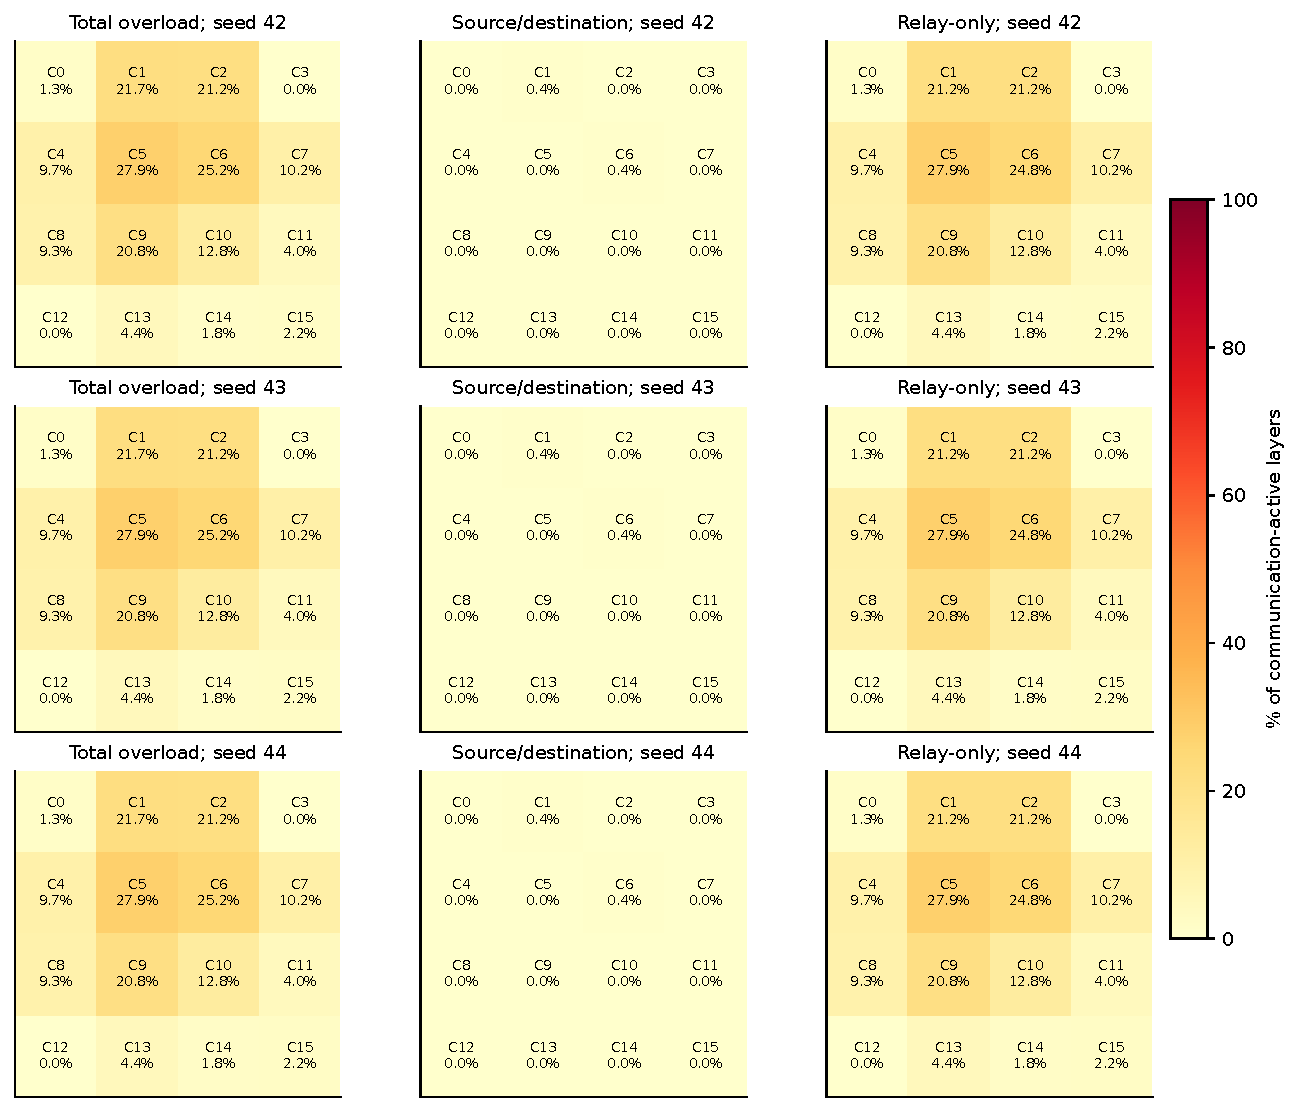
\includegraphics[width=.94\linewidth,height=.48\textheight,keepaspectratio]{figures/atlas/mesh_xy_hop_m4.pdf}\captionof{figure}{All three conceptual mapping seeds; common 0--100 percent colour scale.}\end{center}
\begin{center}{\scriptsize\setlength{\tabcolsep}{3pt}
\begin{tabular}{lrrrrrrrrr}
\toprule
Core & 42 Tot & 42 Own & 42 Rel & 43 Tot & 43 Own & 43 Rel & 44 Tot & 44 Own & 44 Rel \\
\midrule
0 & 1.327 & 0.000 & 1.327 & 1.327 & 0.000 & 1.327 & 1.327 & 0.000 & 1.327 \\
1 & 21.681 & 0.442 & 21.239 & 21.681 & 0.442 & 21.239 & 21.681 & 0.442 & 21.239 \\
2 & 21.239 & 0.000 & 21.239 & 21.239 & 0.000 & 21.239 & 21.239 & 0.000 & 21.239 \\
3 & 0.000 & 0.000 & 0.000 & 0.000 & 0.000 & 0.000 & 0.000 & 0.000 & 0.000 \\
4 & 9.735 & 0.000 & 9.735 & 9.735 & 0.000 & 9.735 & 9.735 & 0.000 & 9.735 \\
5 & 27.876 & 0.000 & 27.876 & 27.876 & 0.000 & 27.876 & 27.876 & 0.000 & 27.876 \\
6 & 25.221 & 0.442 & 24.779 & 25.221 & 0.442 & 24.779 & 25.221 & 0.442 & 24.779 \\
7 & 10.177 & 0.000 & 10.177 & 10.177 & 0.000 & 10.177 & 10.177 & 0.000 & 10.177 \\
8 & 9.292 & 0.000 & 9.292 & 9.292 & 0.000 & 9.292 & 9.292 & 0.000 & 9.292 \\
9 & 20.796 & 0.000 & 20.796 & 20.796 & 0.000 & 20.796 & 20.796 & 0.000 & 20.796 \\
10 & 12.832 & 0.000 & 12.832 & 12.832 & 0.000 & 12.832 & 12.832 & 0.000 & 12.832 \\
11 & 3.982 & 0.000 & 3.982 & 3.982 & 0.000 & 3.982 & 3.982 & 0.000 & 3.982 \\
12 & 0.000 & 0.000 & 0.000 & 0.000 & 0.000 & 0.000 & 0.000 & 0.000 & 0.000 \\
13 & 4.425 & 0.000 & 4.425 & 4.425 & 0.000 & 4.425 & 4.425 & 0.000 & 4.425 \\
14 & 1.770 & 0.000 & 1.770 & 1.770 & 0.000 & 1.770 & 1.770 & 0.000 & 1.770 \\
15 & 2.212 & 0.000 & 2.212 & 2.212 & 0.000 & 2.212 & 2.212 & 0.000 & 2.212 \\
\bottomrule\end{tabular}}
\captionof{table}{Exact heatmap percentages, with Tot = Own + Rel. Unrounded values are in the CSV.}
{\footnotesize\href{https://github.com/sanjeevkrishnaa/Compiler-Driven-ACE/blob/codex/ace-scheduler-correctness/docs/latex/qft96_final/data/heatmap_mesh_xy_hop_m4.csv}{Exact CSV values and sample counts}}
\end{center}
\clearpage\subsection*{Mesh xy; M=6; hop counting}
\begin{center}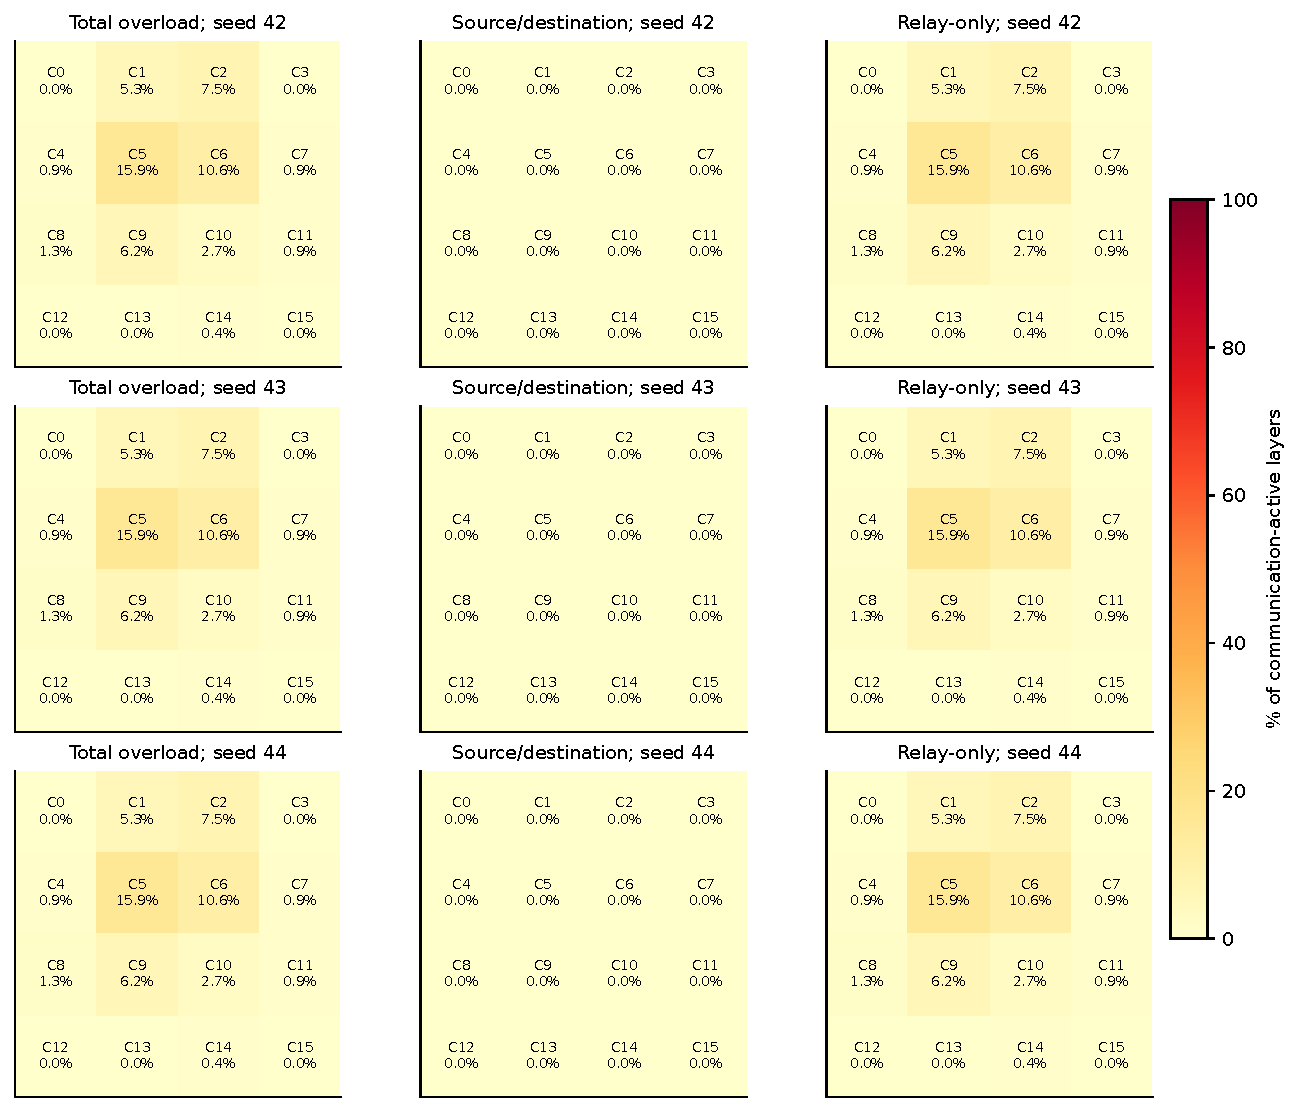
\includegraphics[width=.94\linewidth,height=.48\textheight,keepaspectratio]{figures/atlas/mesh_xy_hop_m6.pdf}\captionof{figure}{All three conceptual mapping seeds; common 0--100 percent colour scale.}\end{center}
\begin{center}{\scriptsize\setlength{\tabcolsep}{3pt}
\begin{tabular}{lrrrrrrrrr}
\toprule
Core & 42 Tot & 42 Own & 42 Rel & 43 Tot & 43 Own & 43 Rel & 44 Tot & 44 Own & 44 Rel \\
\midrule
0 & 0.000 & 0.000 & 0.000 & 0.000 & 0.000 & 0.000 & 0.000 & 0.000 & 0.000 \\
1 & 5.310 & 0.000 & 5.310 & 5.310 & 0.000 & 5.310 & 5.310 & 0.000 & 5.310 \\
2 & 7.522 & 0.000 & 7.522 & 7.522 & 0.000 & 7.522 & 7.522 & 0.000 & 7.522 \\
3 & 0.000 & 0.000 & 0.000 & 0.000 & 0.000 & 0.000 & 0.000 & 0.000 & 0.000 \\
4 & 0.885 & 0.000 & 0.885 & 0.885 & 0.000 & 0.885 & 0.885 & 0.000 & 0.885 \\
5 & 15.929 & 0.000 & 15.929 & 15.929 & 0.000 & 15.929 & 15.929 & 0.000 & 15.929 \\
6 & 10.619 & 0.000 & 10.619 & 10.619 & 0.000 & 10.619 & 10.619 & 0.000 & 10.619 \\
7 & 0.885 & 0.000 & 0.885 & 0.885 & 0.000 & 0.885 & 0.885 & 0.000 & 0.885 \\
8 & 1.327 & 0.000 & 1.327 & 1.327 & 0.000 & 1.327 & 1.327 & 0.000 & 1.327 \\
9 & 6.195 & 0.000 & 6.195 & 6.195 & 0.000 & 6.195 & 6.195 & 0.000 & 6.195 \\
10 & 2.655 & 0.000 & 2.655 & 2.655 & 0.000 & 2.655 & 2.655 & 0.000 & 2.655 \\
11 & 0.885 & 0.000 & 0.885 & 0.885 & 0.000 & 0.885 & 0.885 & 0.000 & 0.885 \\
12 & 0.000 & 0.000 & 0.000 & 0.000 & 0.000 & 0.000 & 0.000 & 0.000 & 0.000 \\
13 & 0.000 & 0.000 & 0.000 & 0.000 & 0.000 & 0.000 & 0.000 & 0.000 & 0.000 \\
14 & 0.442 & 0.000 & 0.442 & 0.442 & 0.000 & 0.442 & 0.442 & 0.000 & 0.442 \\
15 & 0.000 & 0.000 & 0.000 & 0.000 & 0.000 & 0.000 & 0.000 & 0.000 & 0.000 \\
\bottomrule\end{tabular}}
\captionof{table}{Exact heatmap percentages, with Tot = Own + Rel. Unrounded values are in the CSV.}
{\footnotesize\href{https://github.com/sanjeevkrishnaa/Compiler-Driven-ACE/blob/codex/ace-scheduler-correctness/docs/latex/qft96_final/data/heatmap_mesh_xy_hop_m6.csv}{Exact CSV values and sample counts}}
\end{center}
\clearpage\subsection*{Mesh xy; M=8; hop counting}
\begin{center}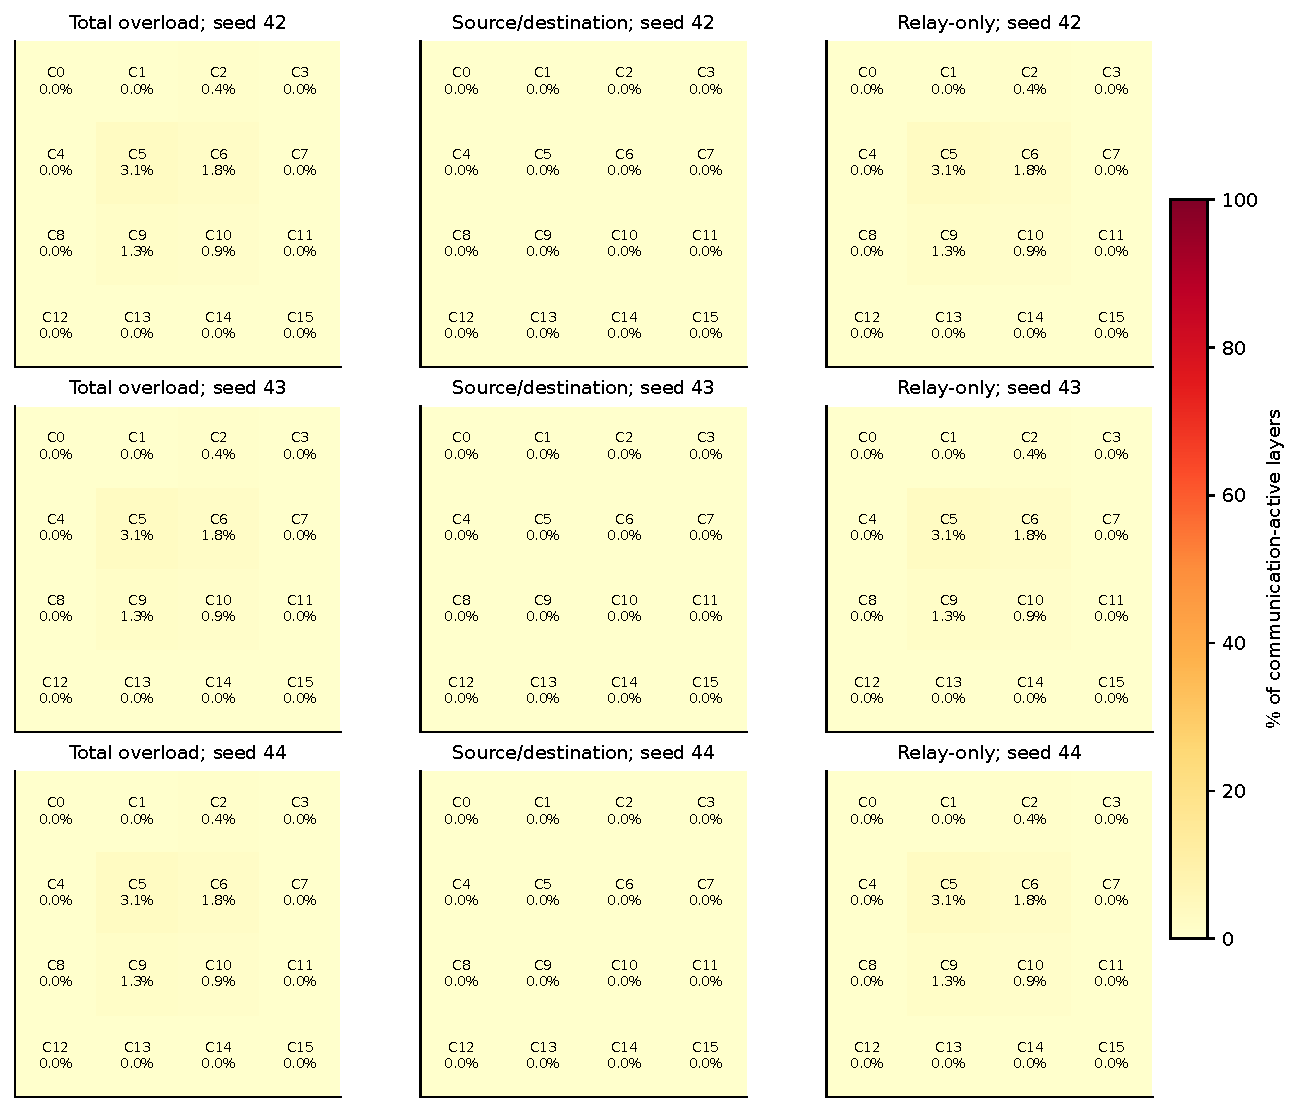
\includegraphics[width=.94\linewidth,height=.48\textheight,keepaspectratio]{figures/atlas/mesh_xy_hop_m8.pdf}\captionof{figure}{All three conceptual mapping seeds; common 0--100 percent colour scale.}\end{center}
\begin{center}{\scriptsize\setlength{\tabcolsep}{3pt}
\begin{tabular}{lrrrrrrrrr}
\toprule
Core & 42 Tot & 42 Own & 42 Rel & 43 Tot & 43 Own & 43 Rel & 44 Tot & 44 Own & 44 Rel \\
\midrule
0 & 0.000 & 0.000 & 0.000 & 0.000 & 0.000 & 0.000 & 0.000 & 0.000 & 0.000 \\
1 & 0.000 & 0.000 & 0.000 & 0.000 & 0.000 & 0.000 & 0.000 & 0.000 & 0.000 \\
2 & 0.442 & 0.000 & 0.442 & 0.442 & 0.000 & 0.442 & 0.442 & 0.000 & 0.442 \\
3 & 0.000 & 0.000 & 0.000 & 0.000 & 0.000 & 0.000 & 0.000 & 0.000 & 0.000 \\
4 & 0.000 & 0.000 & 0.000 & 0.000 & 0.000 & 0.000 & 0.000 & 0.000 & 0.000 \\
5 & 3.097 & 0.000 & 3.097 & 3.097 & 0.000 & 3.097 & 3.097 & 0.000 & 3.097 \\
6 & 1.770 & 0.000 & 1.770 & 1.770 & 0.000 & 1.770 & 1.770 & 0.000 & 1.770 \\
7 & 0.000 & 0.000 & 0.000 & 0.000 & 0.000 & 0.000 & 0.000 & 0.000 & 0.000 \\
8 & 0.000 & 0.000 & 0.000 & 0.000 & 0.000 & 0.000 & 0.000 & 0.000 & 0.000 \\
9 & 1.327 & 0.000 & 1.327 & 1.327 & 0.000 & 1.327 & 1.327 & 0.000 & 1.327 \\
10 & 0.885 & 0.000 & 0.885 & 0.885 & 0.000 & 0.885 & 0.885 & 0.000 & 0.885 \\
11 & 0.000 & 0.000 & 0.000 & 0.000 & 0.000 & 0.000 & 0.000 & 0.000 & 0.000 \\
12 & 0.000 & 0.000 & 0.000 & 0.000 & 0.000 & 0.000 & 0.000 & 0.000 & 0.000 \\
13 & 0.000 & 0.000 & 0.000 & 0.000 & 0.000 & 0.000 & 0.000 & 0.000 & 0.000 \\
14 & 0.000 & 0.000 & 0.000 & 0.000 & 0.000 & 0.000 & 0.000 & 0.000 & 0.000 \\
15 & 0.000 & 0.000 & 0.000 & 0.000 & 0.000 & 0.000 & 0.000 & 0.000 & 0.000 \\
\bottomrule\end{tabular}}
\captionof{table}{Exact heatmap percentages, with Tot = Own + Rel. Unrounded values are in the CSV.}
{\footnotesize\href{https://github.com/sanjeevkrishnaa/Compiler-Driven-ACE/blob/codex/ace-scheduler-correctness/docs/latex/qft96_final/data/heatmap_mesh_xy_hop_m8.csv}{Exact CSV values and sample counts}}
\end{center}
\clearpage\subsection*{Mesh xy; M=16; hop counting}
\begin{center}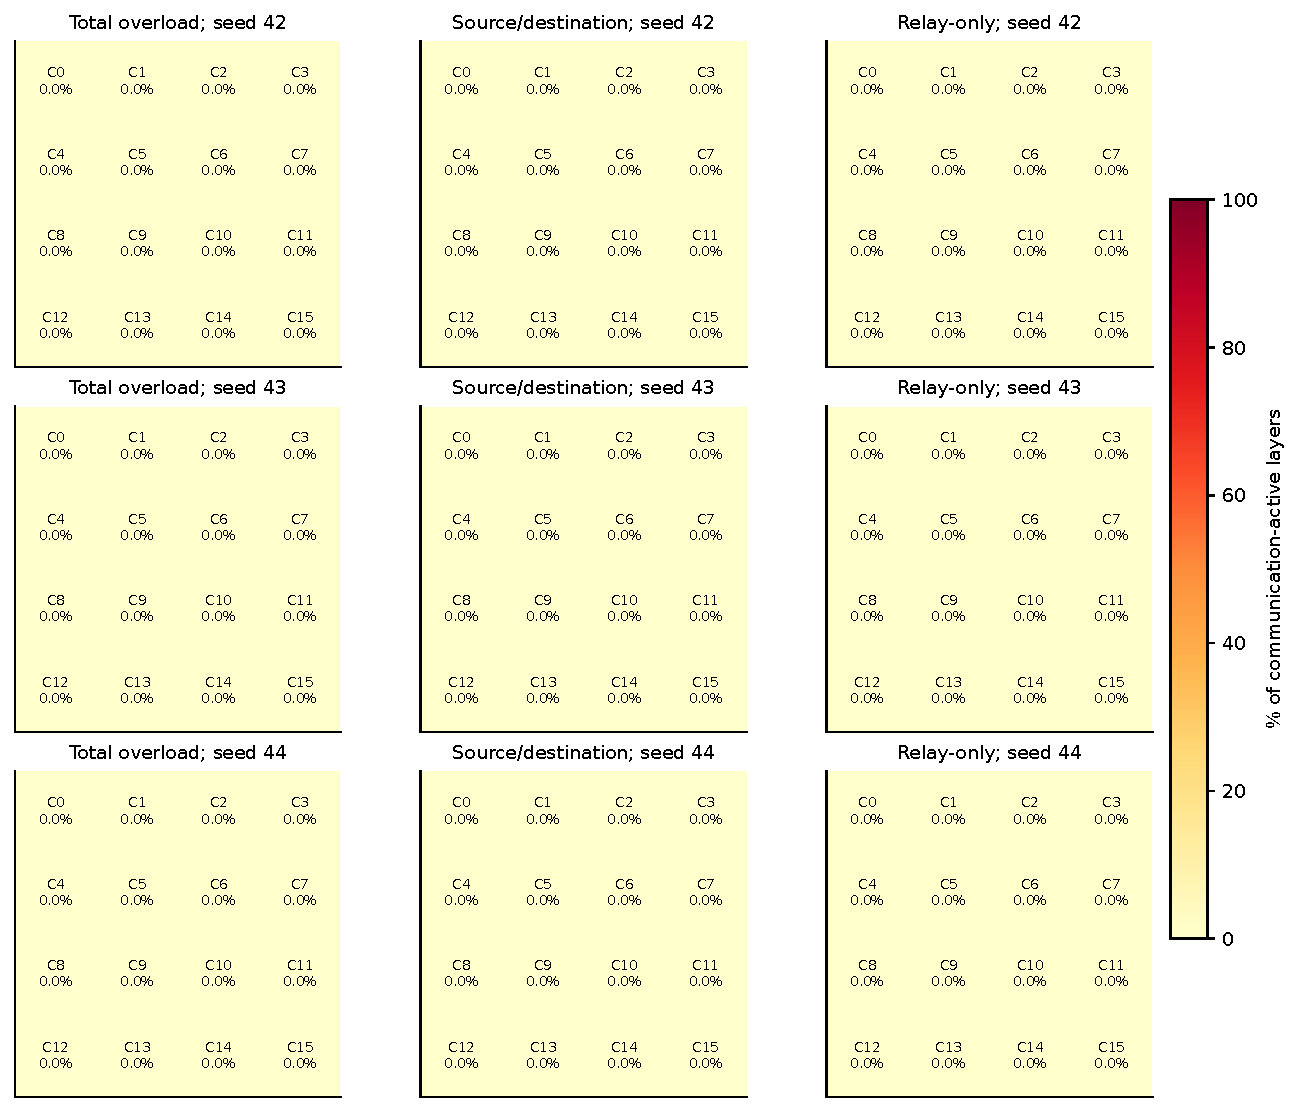
\includegraphics[width=.94\linewidth,height=.48\textheight,keepaspectratio]{figures/atlas/mesh_xy_hop_m16.pdf}\captionof{figure}{All three conceptual mapping seeds; common 0--100 percent colour scale.}\end{center}
\begin{center}{\scriptsize\setlength{\tabcolsep}{3pt}
\begin{tabular}{lrrrrrrrrr}
\toprule
Core & 42 Tot & 42 Own & 42 Rel & 43 Tot & 43 Own & 43 Rel & 44 Tot & 44 Own & 44 Rel \\
\midrule
0 & 0.000 & 0.000 & 0.000 & 0.000 & 0.000 & 0.000 & 0.000 & 0.000 & 0.000 \\
1 & 0.000 & 0.000 & 0.000 & 0.000 & 0.000 & 0.000 & 0.000 & 0.000 & 0.000 \\
2 & 0.000 & 0.000 & 0.000 & 0.000 & 0.000 & 0.000 & 0.000 & 0.000 & 0.000 \\
3 & 0.000 & 0.000 & 0.000 & 0.000 & 0.000 & 0.000 & 0.000 & 0.000 & 0.000 \\
4 & 0.000 & 0.000 & 0.000 & 0.000 & 0.000 & 0.000 & 0.000 & 0.000 & 0.000 \\
5 & 0.000 & 0.000 & 0.000 & 0.000 & 0.000 & 0.000 & 0.000 & 0.000 & 0.000 \\
6 & 0.000 & 0.000 & 0.000 & 0.000 & 0.000 & 0.000 & 0.000 & 0.000 & 0.000 \\
7 & 0.000 & 0.000 & 0.000 & 0.000 & 0.000 & 0.000 & 0.000 & 0.000 & 0.000 \\
8 & 0.000 & 0.000 & 0.000 & 0.000 & 0.000 & 0.000 & 0.000 & 0.000 & 0.000 \\
9 & 0.000 & 0.000 & 0.000 & 0.000 & 0.000 & 0.000 & 0.000 & 0.000 & 0.000 \\
10 & 0.000 & 0.000 & 0.000 & 0.000 & 0.000 & 0.000 & 0.000 & 0.000 & 0.000 \\
11 & 0.000 & 0.000 & 0.000 & 0.000 & 0.000 & 0.000 & 0.000 & 0.000 & 0.000 \\
12 & 0.000 & 0.000 & 0.000 & 0.000 & 0.000 & 0.000 & 0.000 & 0.000 & 0.000 \\
13 & 0.000 & 0.000 & 0.000 & 0.000 & 0.000 & 0.000 & 0.000 & 0.000 & 0.000 \\
14 & 0.000 & 0.000 & 0.000 & 0.000 & 0.000 & 0.000 & 0.000 & 0.000 & 0.000 \\
15 & 0.000 & 0.000 & 0.000 & 0.000 & 0.000 & 0.000 & 0.000 & 0.000 & 0.000 \\
\bottomrule\end{tabular}}
\captionof{table}{Exact heatmap percentages, with Tot = Own + Rel. Unrounded values are in the CSV.}
{\footnotesize\href{https://github.com/sanjeevkrishnaa/Compiler-Driven-ACE/blob/codex/ace-scheduler-correctness/docs/latex/qft96_final/data/heatmap_mesh_xy_hop_m16.csv}{Exact CSV values and sample counts}}
\end{center}
\clearpage\subsection*{Mesh xy; M=32; hop counting}
\begin{center}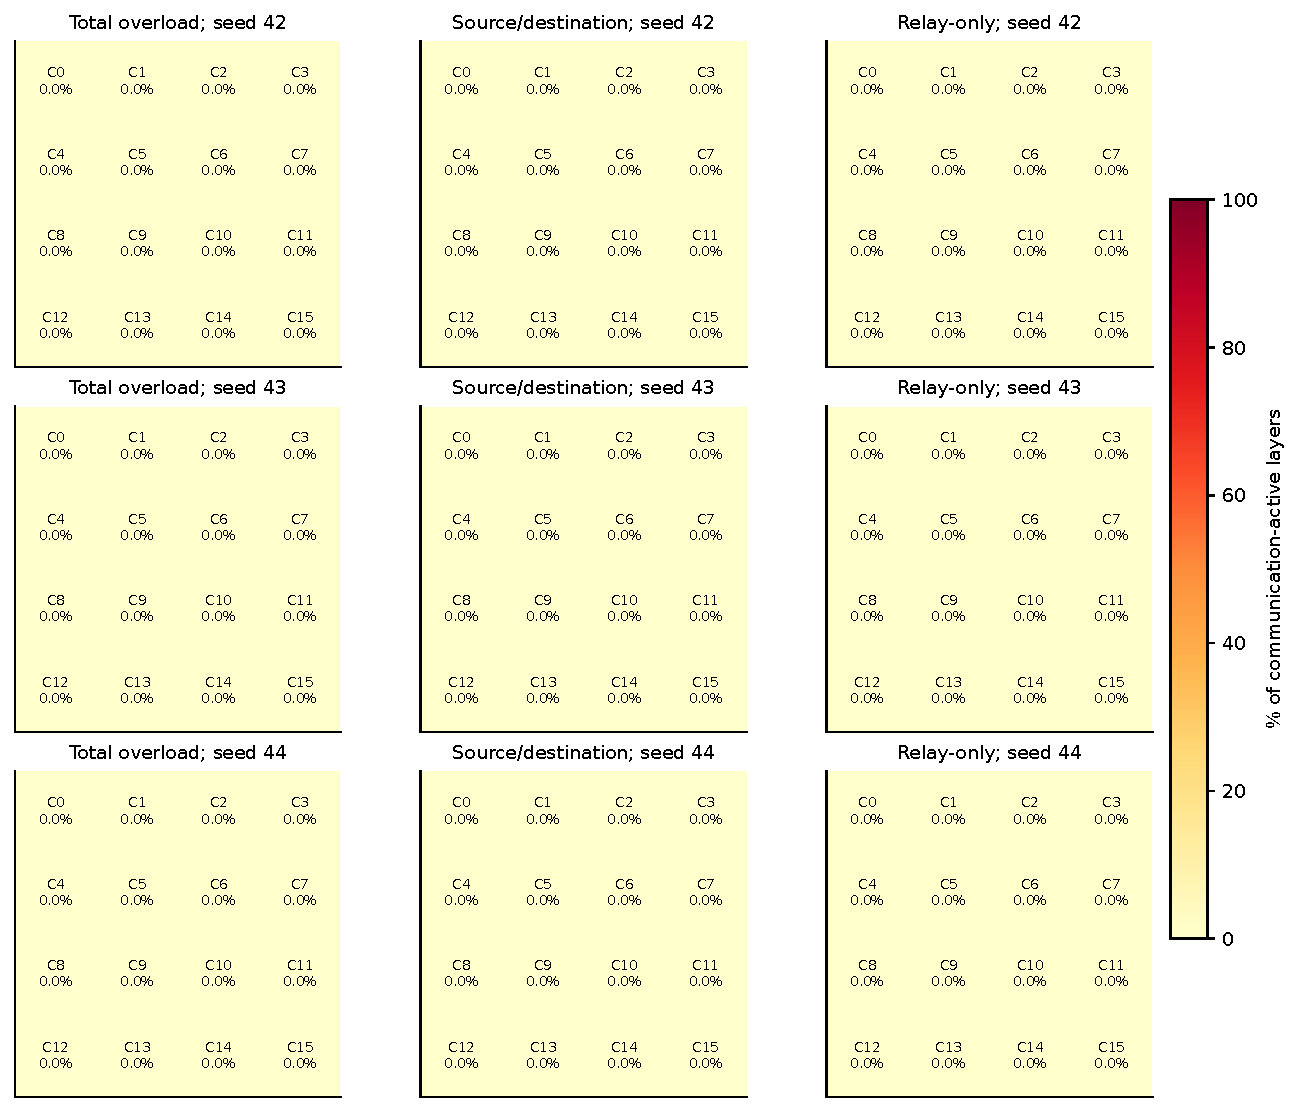
\includegraphics[width=.94\linewidth,height=.48\textheight,keepaspectratio]{figures/atlas/mesh_xy_hop_m32.pdf}\captionof{figure}{All three conceptual mapping seeds; common 0--100 percent colour scale.}\end{center}
\begin{center}{\scriptsize\setlength{\tabcolsep}{3pt}
\begin{tabular}{lrrrrrrrrr}
\toprule
Core & 42 Tot & 42 Own & 42 Rel & 43 Tot & 43 Own & 43 Rel & 44 Tot & 44 Own & 44 Rel \\
\midrule
0 & 0.000 & 0.000 & 0.000 & 0.000 & 0.000 & 0.000 & 0.000 & 0.000 & 0.000 \\
1 & 0.000 & 0.000 & 0.000 & 0.000 & 0.000 & 0.000 & 0.000 & 0.000 & 0.000 \\
2 & 0.000 & 0.000 & 0.000 & 0.000 & 0.000 & 0.000 & 0.000 & 0.000 & 0.000 \\
3 & 0.000 & 0.000 & 0.000 & 0.000 & 0.000 & 0.000 & 0.000 & 0.000 & 0.000 \\
4 & 0.000 & 0.000 & 0.000 & 0.000 & 0.000 & 0.000 & 0.000 & 0.000 & 0.000 \\
5 & 0.000 & 0.000 & 0.000 & 0.000 & 0.000 & 0.000 & 0.000 & 0.000 & 0.000 \\
6 & 0.000 & 0.000 & 0.000 & 0.000 & 0.000 & 0.000 & 0.000 & 0.000 & 0.000 \\
7 & 0.000 & 0.000 & 0.000 & 0.000 & 0.000 & 0.000 & 0.000 & 0.000 & 0.000 \\
8 & 0.000 & 0.000 & 0.000 & 0.000 & 0.000 & 0.000 & 0.000 & 0.000 & 0.000 \\
9 & 0.000 & 0.000 & 0.000 & 0.000 & 0.000 & 0.000 & 0.000 & 0.000 & 0.000 \\
10 & 0.000 & 0.000 & 0.000 & 0.000 & 0.000 & 0.000 & 0.000 & 0.000 & 0.000 \\
11 & 0.000 & 0.000 & 0.000 & 0.000 & 0.000 & 0.000 & 0.000 & 0.000 & 0.000 \\
12 & 0.000 & 0.000 & 0.000 & 0.000 & 0.000 & 0.000 & 0.000 & 0.000 & 0.000 \\
13 & 0.000 & 0.000 & 0.000 & 0.000 & 0.000 & 0.000 & 0.000 & 0.000 & 0.000 \\
14 & 0.000 & 0.000 & 0.000 & 0.000 & 0.000 & 0.000 & 0.000 & 0.000 & 0.000 \\
15 & 0.000 & 0.000 & 0.000 & 0.000 & 0.000 & 0.000 & 0.000 & 0.000 & 0.000 \\
\bottomrule\end{tabular}}
\captionof{table}{Exact heatmap percentages, with Tot = Own + Rel. Unrounded values are in the CSV.}
{\footnotesize\href{https://github.com/sanjeevkrishnaa/Compiler-Driven-ACE/blob/codex/ace-scheduler-correctness/docs/latex/qft96_final/data/heatmap_mesh_xy_hop_m32.csv}{Exact CSV values and sample counts}}
\end{center}
\section{Mesh / yx}
\clearpage\subsection*{Mesh yx; M=2; route counting}
\begin{center}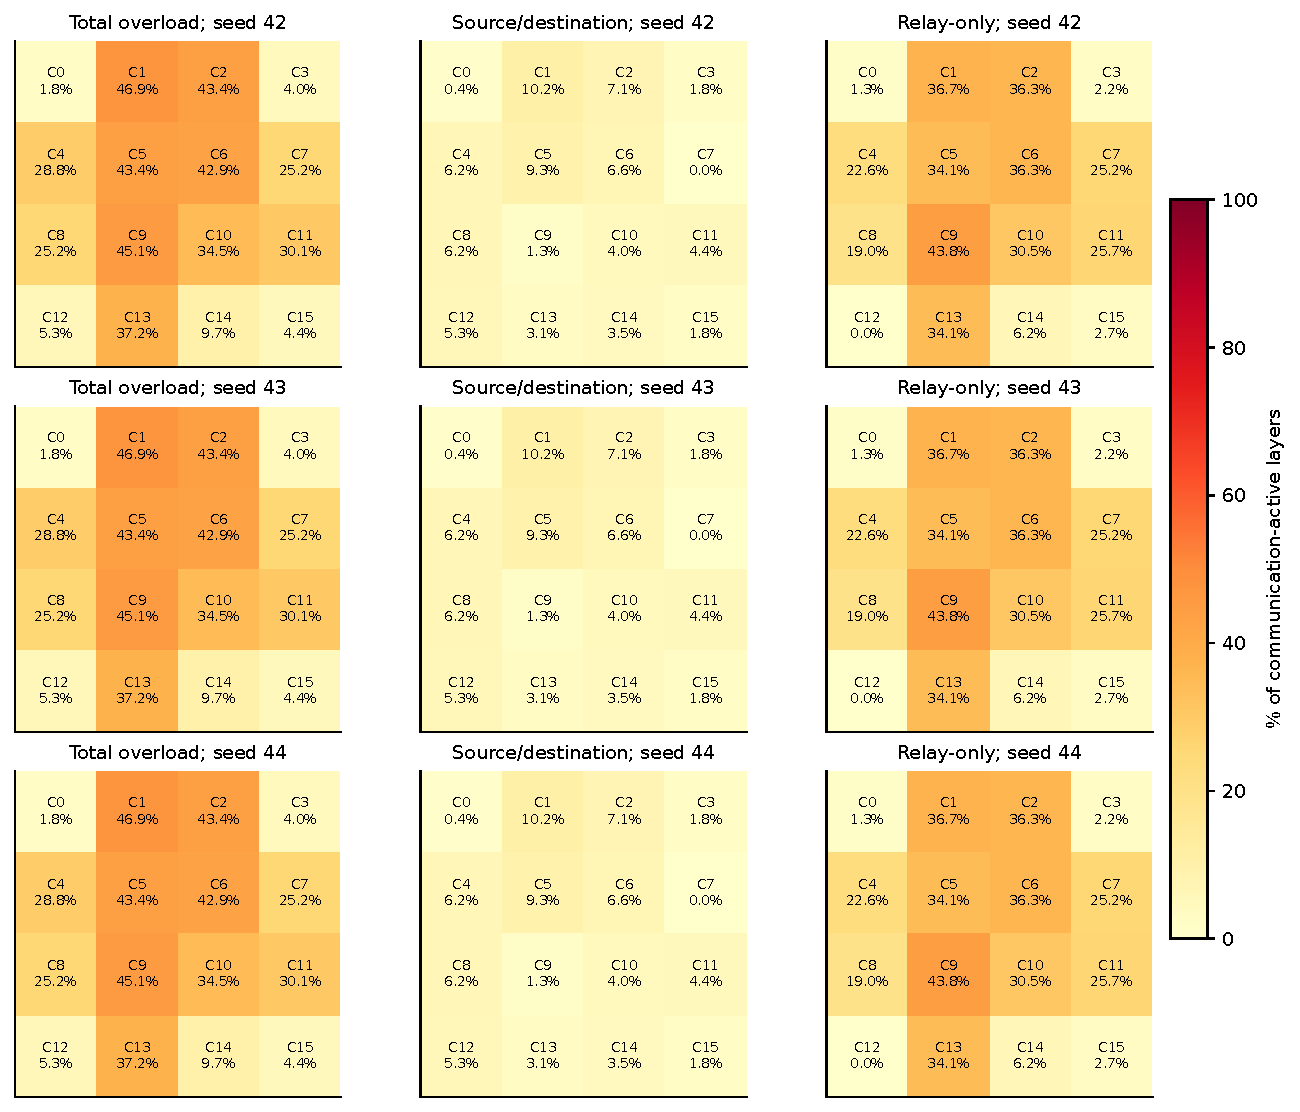
\includegraphics[width=.94\linewidth,height=.48\textheight,keepaspectratio]{figures/atlas/mesh_yx_route_m2.pdf}\captionof{figure}{All three conceptual mapping seeds; common 0--100 percent colour scale.}\end{center}
\begin{center}{\scriptsize\setlength{\tabcolsep}{3pt}
\begin{tabular}{lrrrrrrrrr}
\toprule
Core & 42 Tot & 42 Own & 42 Rel & 43 Tot & 43 Own & 43 Rel & 44 Tot & 44 Own & 44 Rel \\
\midrule
0 & 1.770 & 0.442 & 1.327 & 1.770 & 0.442 & 1.327 & 1.770 & 0.442 & 1.327 \\
1 & 46.903 & 10.177 & 36.726 & 46.903 & 10.177 & 36.726 & 46.903 & 10.177 & 36.726 \\
2 & 43.363 & 7.080 & 36.283 & 43.363 & 7.080 & 36.283 & 43.363 & 7.080 & 36.283 \\
3 & 3.982 & 1.770 & 2.212 & 3.982 & 1.770 & 2.212 & 3.982 & 1.770 & 2.212 \\
4 & 28.761 & 6.195 & 22.566 & 28.761 & 6.195 & 22.566 & 28.761 & 6.195 & 22.566 \\
5 & 43.363 & 9.292 & 34.071 & 43.363 & 9.292 & 34.071 & 43.363 & 9.292 & 34.071 \\
6 & 42.920 & 6.637 & 36.283 & 42.920 & 6.637 & 36.283 & 42.920 & 6.637 & 36.283 \\
7 & 25.221 & 0.000 & 25.221 & 25.221 & 0.000 & 25.221 & 25.221 & 0.000 & 25.221 \\
8 & 25.221 & 6.195 & 19.027 & 25.221 & 6.195 & 19.027 & 25.221 & 6.195 & 19.027 \\
9 & 45.133 & 1.327 & 43.805 & 45.133 & 1.327 & 43.805 & 45.133 & 1.327 & 43.805 \\
10 & 34.513 & 3.982 & 30.531 & 34.513 & 3.982 & 30.531 & 34.513 & 3.982 & 30.531 \\
11 & 30.088 & 4.425 & 25.664 & 30.088 & 4.425 & 25.664 & 30.088 & 4.425 & 25.664 \\
12 & 5.310 & 5.310 & 0.000 & 5.310 & 5.310 & 0.000 & 5.310 & 5.310 & 0.000 \\
13 & 37.168 & 3.097 & 34.071 & 37.168 & 3.097 & 34.071 & 37.168 & 3.097 & 34.071 \\
14 & 9.735 & 3.540 & 6.195 & 9.735 & 3.540 & 6.195 & 9.735 & 3.540 & 6.195 \\
15 & 4.425 & 1.770 & 2.655 & 4.425 & 1.770 & 2.655 & 4.425 & 1.770 & 2.655 \\
\bottomrule\end{tabular}}
\captionof{table}{Exact heatmap percentages, with Tot = Own + Rel. Unrounded values are in the CSV.}
{\footnotesize\href{https://github.com/sanjeevkrishnaa/Compiler-Driven-ACE/blob/codex/ace-scheduler-correctness/docs/latex/qft96_final/data/heatmap_mesh_yx_route_m2.csv}{Exact CSV values and sample counts}}
\end{center}
\clearpage\subsection*{Mesh yx; M=3; route counting}
\begin{center}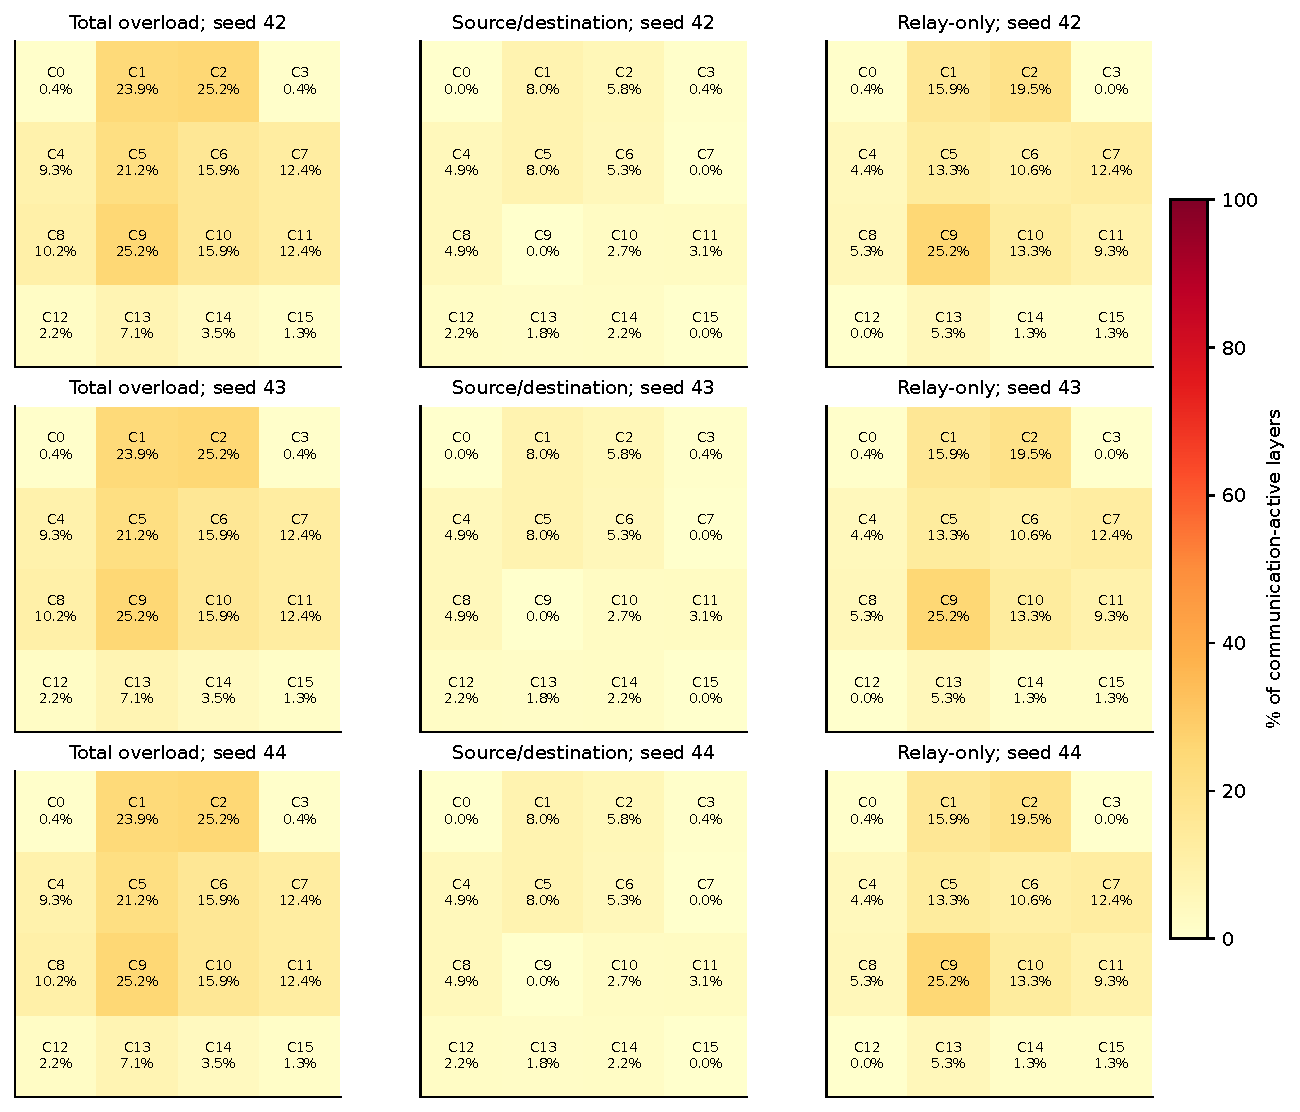
\includegraphics[width=.94\linewidth,height=.48\textheight,keepaspectratio]{figures/atlas/mesh_yx_route_m3.pdf}\captionof{figure}{All three conceptual mapping seeds; common 0--100 percent colour scale.}\end{center}
\begin{center}{\scriptsize\setlength{\tabcolsep}{3pt}
\begin{tabular}{lrrrrrrrrr}
\toprule
Core & 42 Tot & 42 Own & 42 Rel & 43 Tot & 43 Own & 43 Rel & 44 Tot & 44 Own & 44 Rel \\
\midrule
0 & 0.442 & 0.000 & 0.442 & 0.442 & 0.000 & 0.442 & 0.442 & 0.000 & 0.442 \\
1 & 23.894 & 7.965 & 15.929 & 23.894 & 7.965 & 15.929 & 23.894 & 7.965 & 15.929 \\
2 & 25.221 & 5.752 & 19.469 & 25.221 & 5.752 & 19.469 & 25.221 & 5.752 & 19.469 \\
3 & 0.442 & 0.442 & 0.000 & 0.442 & 0.442 & 0.000 & 0.442 & 0.442 & 0.000 \\
4 & 9.292 & 4.867 & 4.425 & 9.292 & 4.867 & 4.425 & 9.292 & 4.867 & 4.425 \\
5 & 21.239 & 7.965 & 13.274 & 21.239 & 7.965 & 13.274 & 21.239 & 7.965 & 13.274 \\
6 & 15.929 & 5.310 & 10.619 & 15.929 & 5.310 & 10.619 & 15.929 & 5.310 & 10.619 \\
7 & 12.389 & 0.000 & 12.389 & 12.389 & 0.000 & 12.389 & 12.389 & 0.000 & 12.389 \\
8 & 10.177 & 4.867 & 5.310 & 10.177 & 4.867 & 5.310 & 10.177 & 4.867 & 5.310 \\
9 & 25.221 & 0.000 & 25.221 & 25.221 & 0.000 & 25.221 & 25.221 & 0.000 & 25.221 \\
10 & 15.929 & 2.655 & 13.274 & 15.929 & 2.655 & 13.274 & 15.929 & 2.655 & 13.274 \\
11 & 12.389 & 3.097 & 9.292 & 12.389 & 3.097 & 9.292 & 12.389 & 3.097 & 9.292 \\
12 & 2.212 & 2.212 & 0.000 & 2.212 & 2.212 & 0.000 & 2.212 & 2.212 & 0.000 \\
13 & 7.080 & 1.770 & 5.310 & 7.080 & 1.770 & 5.310 & 7.080 & 1.770 & 5.310 \\
14 & 3.540 & 2.212 & 1.327 & 3.540 & 2.212 & 1.327 & 3.540 & 2.212 & 1.327 \\
15 & 1.327 & 0.000 & 1.327 & 1.327 & 0.000 & 1.327 & 1.327 & 0.000 & 1.327 \\
\bottomrule\end{tabular}}
\captionof{table}{Exact heatmap percentages, with Tot = Own + Rel. Unrounded values are in the CSV.}
{\footnotesize\href{https://github.com/sanjeevkrishnaa/Compiler-Driven-ACE/blob/codex/ace-scheduler-correctness/docs/latex/qft96_final/data/heatmap_mesh_yx_route_m3.csv}{Exact CSV values and sample counts}}
\end{center}
\clearpage\subsection*{Mesh yx; M=4; route counting}
\begin{center}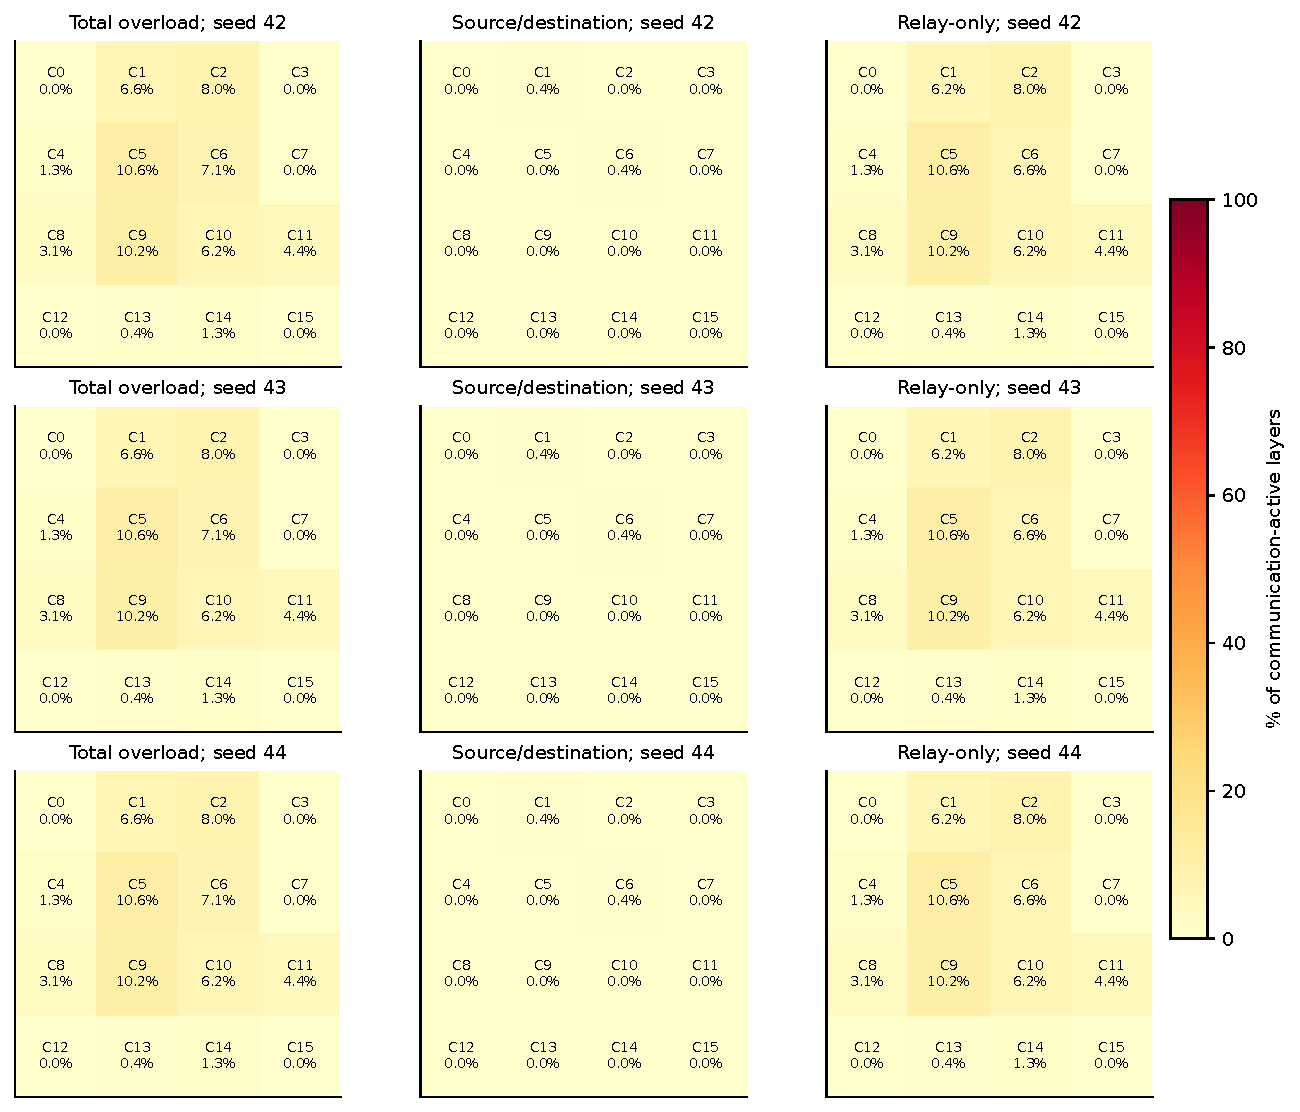
\includegraphics[width=.94\linewidth,height=.48\textheight,keepaspectratio]{figures/atlas/mesh_yx_route_m4.pdf}\captionof{figure}{All three conceptual mapping seeds; common 0--100 percent colour scale.}\end{center}
\begin{center}{\scriptsize\setlength{\tabcolsep}{3pt}
\begin{tabular}{lrrrrrrrrr}
\toprule
Core & 42 Tot & 42 Own & 42 Rel & 43 Tot & 43 Own & 43 Rel & 44 Tot & 44 Own & 44 Rel \\
\midrule
0 & 0.000 & 0.000 & 0.000 & 0.000 & 0.000 & 0.000 & 0.000 & 0.000 & 0.000 \\
1 & 6.637 & 0.442 & 6.195 & 6.637 & 0.442 & 6.195 & 6.637 & 0.442 & 6.195 \\
2 & 7.965 & 0.000 & 7.965 & 7.965 & 0.000 & 7.965 & 7.965 & 0.000 & 7.965 \\
3 & 0.000 & 0.000 & 0.000 & 0.000 & 0.000 & 0.000 & 0.000 & 0.000 & 0.000 \\
4 & 1.327 & 0.000 & 1.327 & 1.327 & 0.000 & 1.327 & 1.327 & 0.000 & 1.327 \\
5 & 10.619 & 0.000 & 10.619 & 10.619 & 0.000 & 10.619 & 10.619 & 0.000 & 10.619 \\
6 & 7.080 & 0.442 & 6.637 & 7.080 & 0.442 & 6.637 & 7.080 & 0.442 & 6.637 \\
7 & 0.000 & 0.000 & 0.000 & 0.000 & 0.000 & 0.000 & 0.000 & 0.000 & 0.000 \\
8 & 3.097 & 0.000 & 3.097 & 3.097 & 0.000 & 3.097 & 3.097 & 0.000 & 3.097 \\
9 & 10.177 & 0.000 & 10.177 & 10.177 & 0.000 & 10.177 & 10.177 & 0.000 & 10.177 \\
10 & 6.195 & 0.000 & 6.195 & 6.195 & 0.000 & 6.195 & 6.195 & 0.000 & 6.195 \\
11 & 4.425 & 0.000 & 4.425 & 4.425 & 0.000 & 4.425 & 4.425 & 0.000 & 4.425 \\
12 & 0.000 & 0.000 & 0.000 & 0.000 & 0.000 & 0.000 & 0.000 & 0.000 & 0.000 \\
13 & 0.442 & 0.000 & 0.442 & 0.442 & 0.000 & 0.442 & 0.442 & 0.000 & 0.442 \\
14 & 1.327 & 0.000 & 1.327 & 1.327 & 0.000 & 1.327 & 1.327 & 0.000 & 1.327 \\
15 & 0.000 & 0.000 & 0.000 & 0.000 & 0.000 & 0.000 & 0.000 & 0.000 & 0.000 \\
\bottomrule\end{tabular}}
\captionof{table}{Exact heatmap percentages, with Tot = Own + Rel. Unrounded values are in the CSV.}
{\footnotesize\href{https://github.com/sanjeevkrishnaa/Compiler-Driven-ACE/blob/codex/ace-scheduler-correctness/docs/latex/qft96_final/data/heatmap_mesh_yx_route_m4.csv}{Exact CSV values and sample counts}}
\end{center}
\clearpage\subsection*{Mesh yx; M=6; route counting}
\begin{center}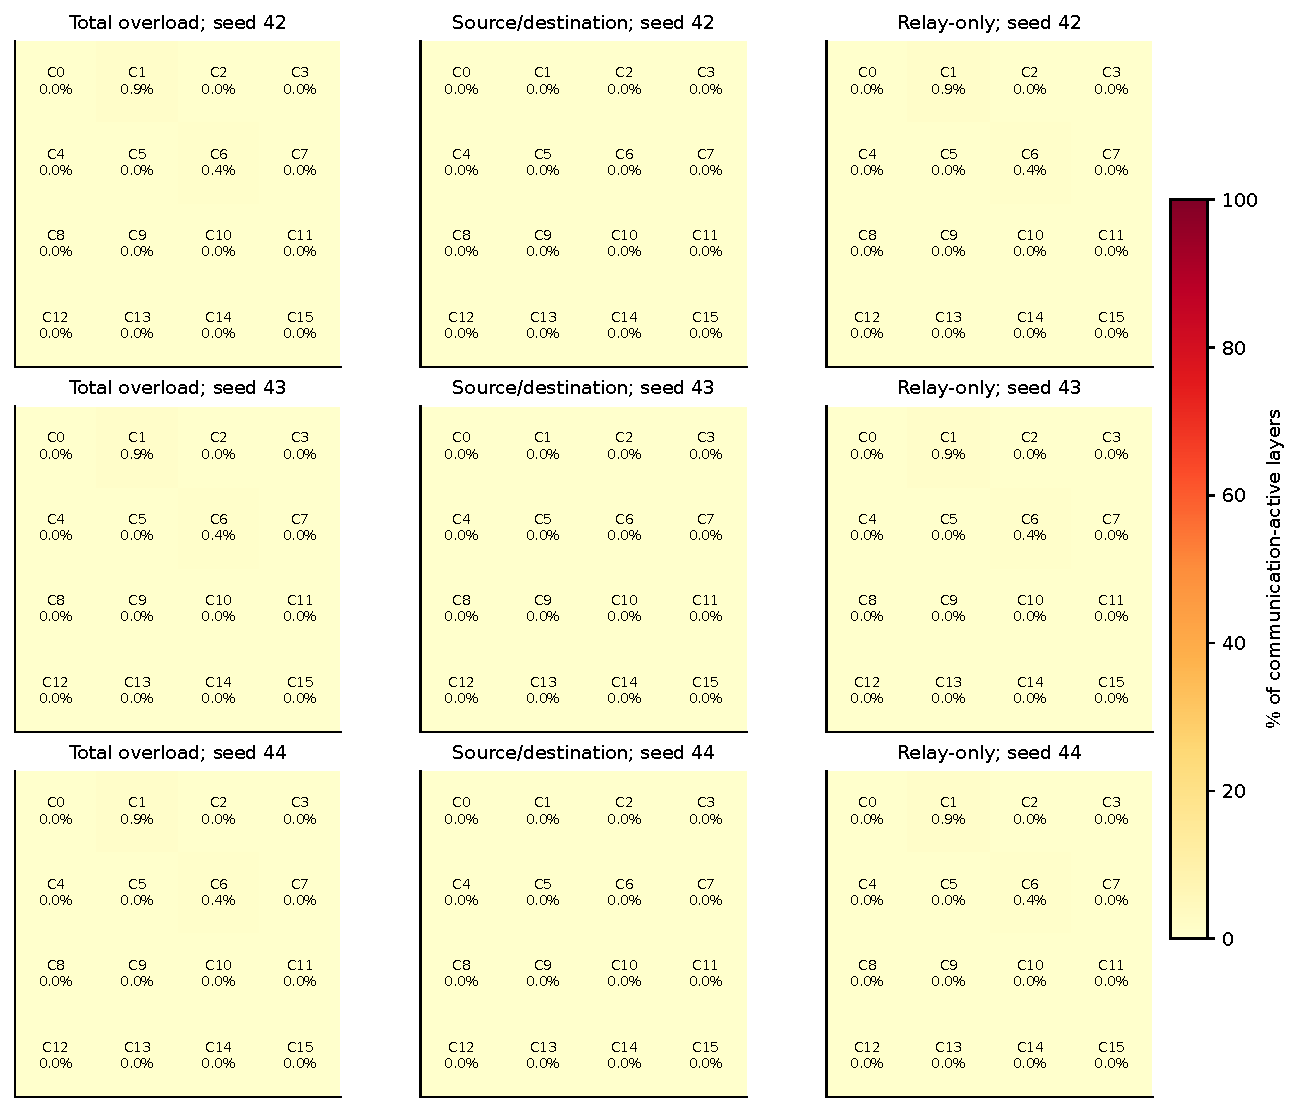
\includegraphics[width=.94\linewidth,height=.48\textheight,keepaspectratio]{figures/atlas/mesh_yx_route_m6.pdf}\captionof{figure}{All three conceptual mapping seeds; common 0--100 percent colour scale.}\end{center}
\begin{center}{\scriptsize\setlength{\tabcolsep}{3pt}
\begin{tabular}{lrrrrrrrrr}
\toprule
Core & 42 Tot & 42 Own & 42 Rel & 43 Tot & 43 Own & 43 Rel & 44 Tot & 44 Own & 44 Rel \\
\midrule
0 & 0.000 & 0.000 & 0.000 & 0.000 & 0.000 & 0.000 & 0.000 & 0.000 & 0.000 \\
1 & 0.885 & 0.000 & 0.885 & 0.885 & 0.000 & 0.885 & 0.885 & 0.000 & 0.885 \\
2 & 0.000 & 0.000 & 0.000 & 0.000 & 0.000 & 0.000 & 0.000 & 0.000 & 0.000 \\
3 & 0.000 & 0.000 & 0.000 & 0.000 & 0.000 & 0.000 & 0.000 & 0.000 & 0.000 \\
4 & 0.000 & 0.000 & 0.000 & 0.000 & 0.000 & 0.000 & 0.000 & 0.000 & 0.000 \\
5 & 0.000 & 0.000 & 0.000 & 0.000 & 0.000 & 0.000 & 0.000 & 0.000 & 0.000 \\
6 & 0.442 & 0.000 & 0.442 & 0.442 & 0.000 & 0.442 & 0.442 & 0.000 & 0.442 \\
7 & 0.000 & 0.000 & 0.000 & 0.000 & 0.000 & 0.000 & 0.000 & 0.000 & 0.000 \\
8 & 0.000 & 0.000 & 0.000 & 0.000 & 0.000 & 0.000 & 0.000 & 0.000 & 0.000 \\
9 & 0.000 & 0.000 & 0.000 & 0.000 & 0.000 & 0.000 & 0.000 & 0.000 & 0.000 \\
10 & 0.000 & 0.000 & 0.000 & 0.000 & 0.000 & 0.000 & 0.000 & 0.000 & 0.000 \\
11 & 0.000 & 0.000 & 0.000 & 0.000 & 0.000 & 0.000 & 0.000 & 0.000 & 0.000 \\
12 & 0.000 & 0.000 & 0.000 & 0.000 & 0.000 & 0.000 & 0.000 & 0.000 & 0.000 \\
13 & 0.000 & 0.000 & 0.000 & 0.000 & 0.000 & 0.000 & 0.000 & 0.000 & 0.000 \\
14 & 0.000 & 0.000 & 0.000 & 0.000 & 0.000 & 0.000 & 0.000 & 0.000 & 0.000 \\
15 & 0.000 & 0.000 & 0.000 & 0.000 & 0.000 & 0.000 & 0.000 & 0.000 & 0.000 \\
\bottomrule\end{tabular}}
\captionof{table}{Exact heatmap percentages, with Tot = Own + Rel. Unrounded values are in the CSV.}
{\footnotesize\href{https://github.com/sanjeevkrishnaa/Compiler-Driven-ACE/blob/codex/ace-scheduler-correctness/docs/latex/qft96_final/data/heatmap_mesh_yx_route_m6.csv}{Exact CSV values and sample counts}}
\end{center}
\clearpage\subsection*{Mesh yx; M=8; route counting}
\begin{center}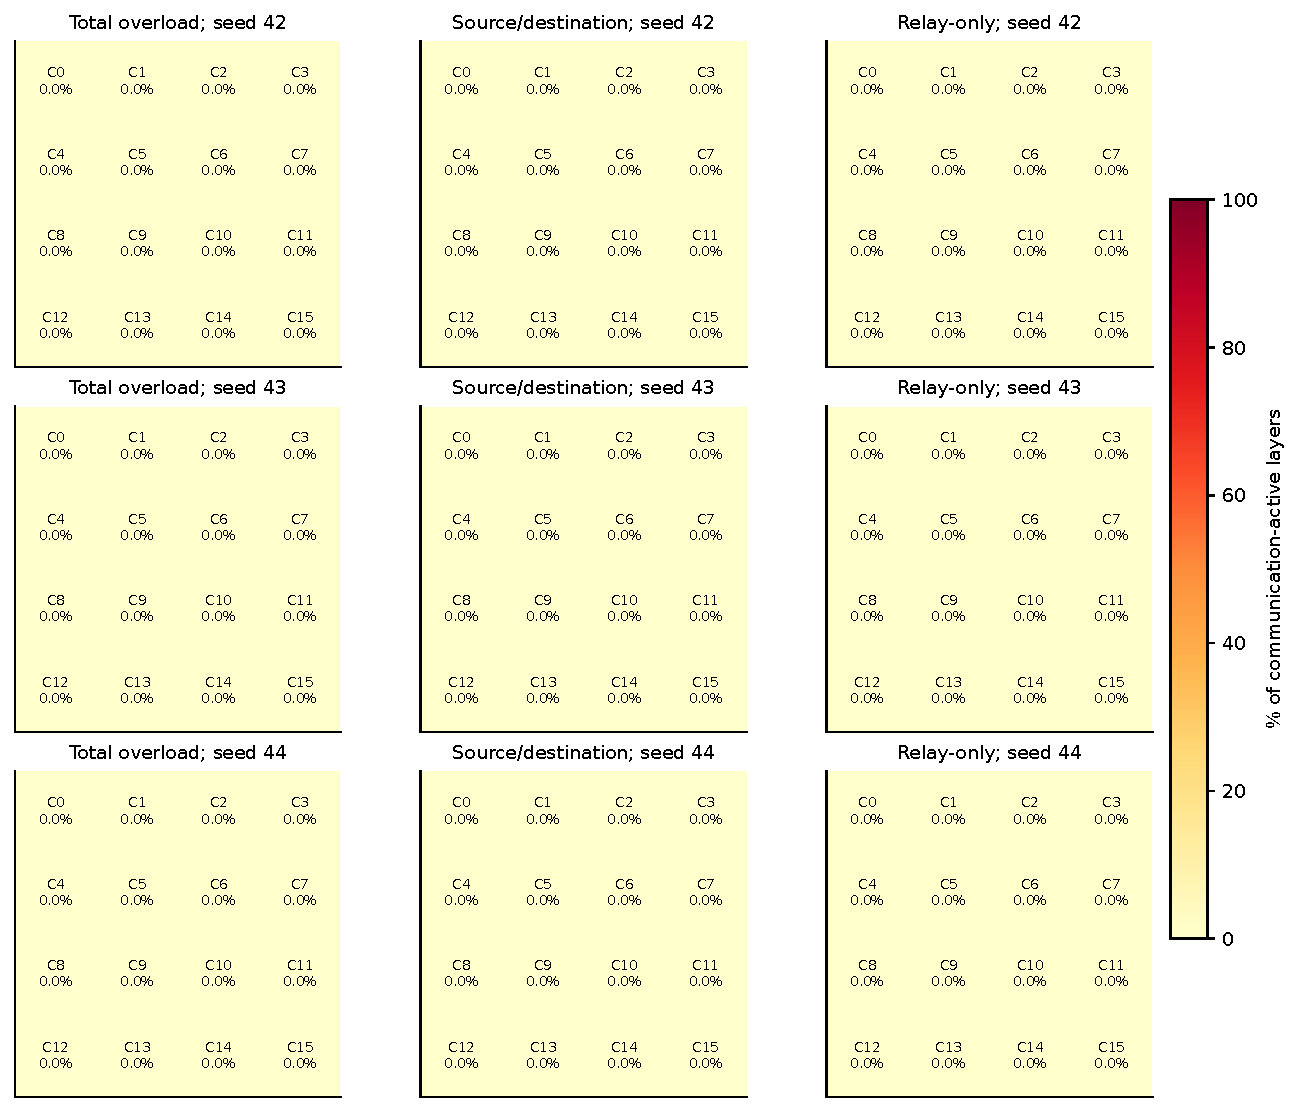
\includegraphics[width=.94\linewidth,height=.48\textheight,keepaspectratio]{figures/atlas/mesh_yx_route_m8.pdf}\captionof{figure}{All three conceptual mapping seeds; common 0--100 percent colour scale.}\end{center}
\begin{center}{\scriptsize\setlength{\tabcolsep}{3pt}
\begin{tabular}{lrrrrrrrrr}
\toprule
Core & 42 Tot & 42 Own & 42 Rel & 43 Tot & 43 Own & 43 Rel & 44 Tot & 44 Own & 44 Rel \\
\midrule
0 & 0.000 & 0.000 & 0.000 & 0.000 & 0.000 & 0.000 & 0.000 & 0.000 & 0.000 \\
1 & 0.000 & 0.000 & 0.000 & 0.000 & 0.000 & 0.000 & 0.000 & 0.000 & 0.000 \\
2 & 0.000 & 0.000 & 0.000 & 0.000 & 0.000 & 0.000 & 0.000 & 0.000 & 0.000 \\
3 & 0.000 & 0.000 & 0.000 & 0.000 & 0.000 & 0.000 & 0.000 & 0.000 & 0.000 \\
4 & 0.000 & 0.000 & 0.000 & 0.000 & 0.000 & 0.000 & 0.000 & 0.000 & 0.000 \\
5 & 0.000 & 0.000 & 0.000 & 0.000 & 0.000 & 0.000 & 0.000 & 0.000 & 0.000 \\
6 & 0.000 & 0.000 & 0.000 & 0.000 & 0.000 & 0.000 & 0.000 & 0.000 & 0.000 \\
7 & 0.000 & 0.000 & 0.000 & 0.000 & 0.000 & 0.000 & 0.000 & 0.000 & 0.000 \\
8 & 0.000 & 0.000 & 0.000 & 0.000 & 0.000 & 0.000 & 0.000 & 0.000 & 0.000 \\
9 & 0.000 & 0.000 & 0.000 & 0.000 & 0.000 & 0.000 & 0.000 & 0.000 & 0.000 \\
10 & 0.000 & 0.000 & 0.000 & 0.000 & 0.000 & 0.000 & 0.000 & 0.000 & 0.000 \\
11 & 0.000 & 0.000 & 0.000 & 0.000 & 0.000 & 0.000 & 0.000 & 0.000 & 0.000 \\
12 & 0.000 & 0.000 & 0.000 & 0.000 & 0.000 & 0.000 & 0.000 & 0.000 & 0.000 \\
13 & 0.000 & 0.000 & 0.000 & 0.000 & 0.000 & 0.000 & 0.000 & 0.000 & 0.000 \\
14 & 0.000 & 0.000 & 0.000 & 0.000 & 0.000 & 0.000 & 0.000 & 0.000 & 0.000 \\
15 & 0.000 & 0.000 & 0.000 & 0.000 & 0.000 & 0.000 & 0.000 & 0.000 & 0.000 \\
\bottomrule\end{tabular}}
\captionof{table}{Exact heatmap percentages, with Tot = Own + Rel. Unrounded values are in the CSV.}
{\footnotesize\href{https://github.com/sanjeevkrishnaa/Compiler-Driven-ACE/blob/codex/ace-scheduler-correctness/docs/latex/qft96_final/data/heatmap_mesh_yx_route_m8.csv}{Exact CSV values and sample counts}}
\end{center}
\clearpage\subsection*{Mesh yx; M=16; route counting}
\begin{center}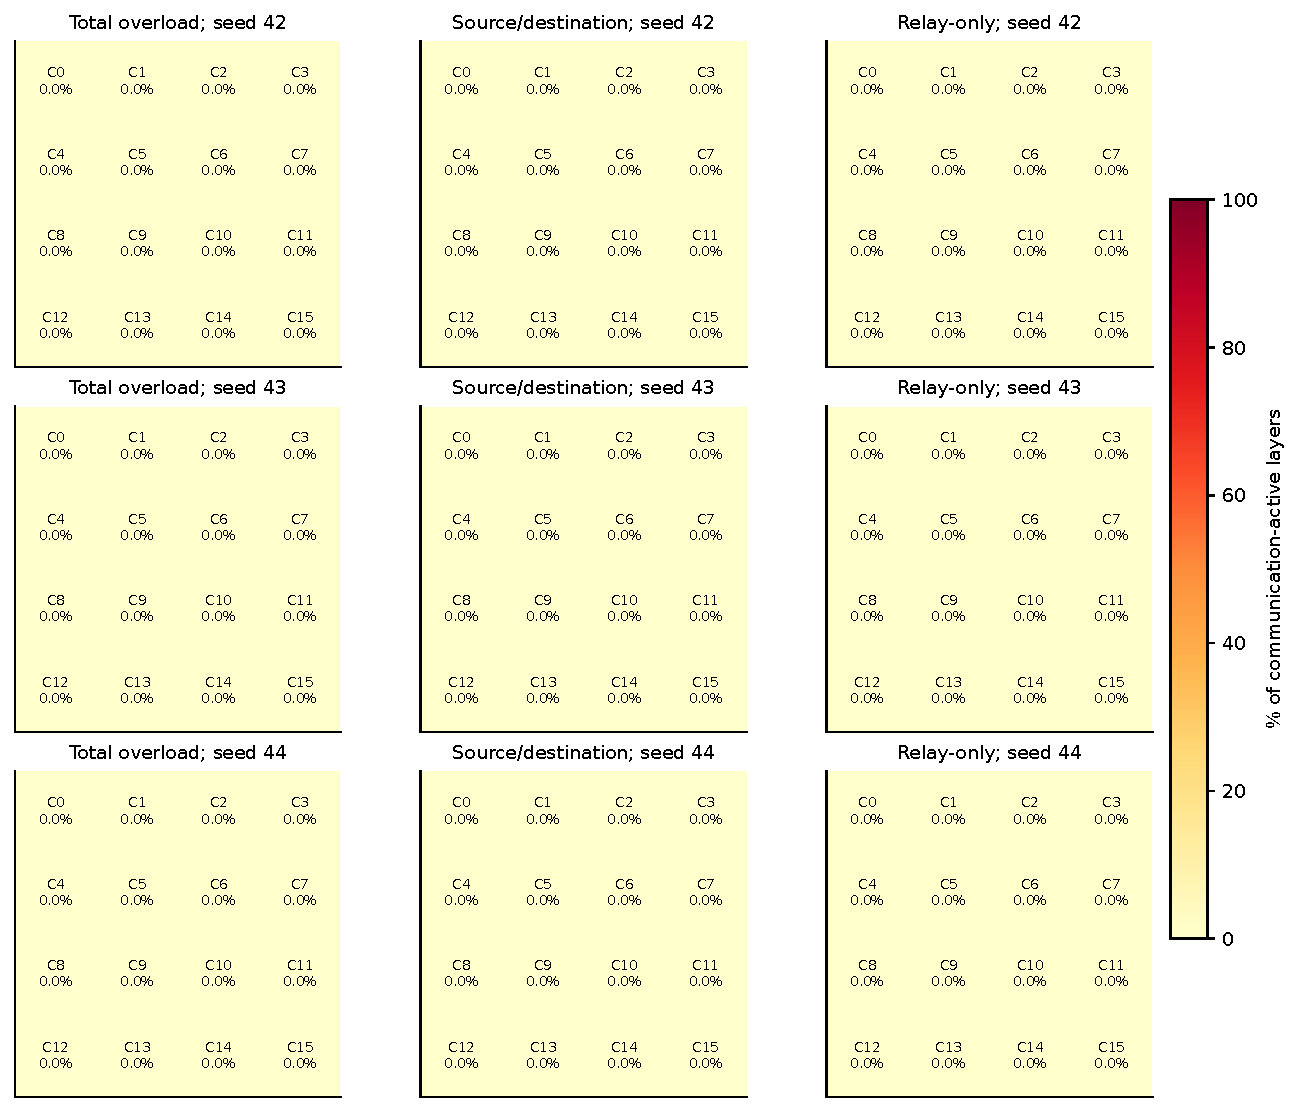
\includegraphics[width=.94\linewidth,height=.48\textheight,keepaspectratio]{figures/atlas/mesh_yx_route_m16.pdf}\captionof{figure}{All three conceptual mapping seeds; common 0--100 percent colour scale.}\end{center}
\begin{center}{\scriptsize\setlength{\tabcolsep}{3pt}
\begin{tabular}{lrrrrrrrrr}
\toprule
Core & 42 Tot & 42 Own & 42 Rel & 43 Tot & 43 Own & 43 Rel & 44 Tot & 44 Own & 44 Rel \\
\midrule
0 & 0.000 & 0.000 & 0.000 & 0.000 & 0.000 & 0.000 & 0.000 & 0.000 & 0.000 \\
1 & 0.000 & 0.000 & 0.000 & 0.000 & 0.000 & 0.000 & 0.000 & 0.000 & 0.000 \\
2 & 0.000 & 0.000 & 0.000 & 0.000 & 0.000 & 0.000 & 0.000 & 0.000 & 0.000 \\
3 & 0.000 & 0.000 & 0.000 & 0.000 & 0.000 & 0.000 & 0.000 & 0.000 & 0.000 \\
4 & 0.000 & 0.000 & 0.000 & 0.000 & 0.000 & 0.000 & 0.000 & 0.000 & 0.000 \\
5 & 0.000 & 0.000 & 0.000 & 0.000 & 0.000 & 0.000 & 0.000 & 0.000 & 0.000 \\
6 & 0.000 & 0.000 & 0.000 & 0.000 & 0.000 & 0.000 & 0.000 & 0.000 & 0.000 \\
7 & 0.000 & 0.000 & 0.000 & 0.000 & 0.000 & 0.000 & 0.000 & 0.000 & 0.000 \\
8 & 0.000 & 0.000 & 0.000 & 0.000 & 0.000 & 0.000 & 0.000 & 0.000 & 0.000 \\
9 & 0.000 & 0.000 & 0.000 & 0.000 & 0.000 & 0.000 & 0.000 & 0.000 & 0.000 \\
10 & 0.000 & 0.000 & 0.000 & 0.000 & 0.000 & 0.000 & 0.000 & 0.000 & 0.000 \\
11 & 0.000 & 0.000 & 0.000 & 0.000 & 0.000 & 0.000 & 0.000 & 0.000 & 0.000 \\
12 & 0.000 & 0.000 & 0.000 & 0.000 & 0.000 & 0.000 & 0.000 & 0.000 & 0.000 \\
13 & 0.000 & 0.000 & 0.000 & 0.000 & 0.000 & 0.000 & 0.000 & 0.000 & 0.000 \\
14 & 0.000 & 0.000 & 0.000 & 0.000 & 0.000 & 0.000 & 0.000 & 0.000 & 0.000 \\
15 & 0.000 & 0.000 & 0.000 & 0.000 & 0.000 & 0.000 & 0.000 & 0.000 & 0.000 \\
\bottomrule\end{tabular}}
\captionof{table}{Exact heatmap percentages, with Tot = Own + Rel. Unrounded values are in the CSV.}
{\footnotesize\href{https://github.com/sanjeevkrishnaa/Compiler-Driven-ACE/blob/codex/ace-scheduler-correctness/docs/latex/qft96_final/data/heatmap_mesh_yx_route_m16.csv}{Exact CSV values and sample counts}}
\end{center}
\clearpage\subsection*{Mesh yx; M=32; route counting}
\begin{center}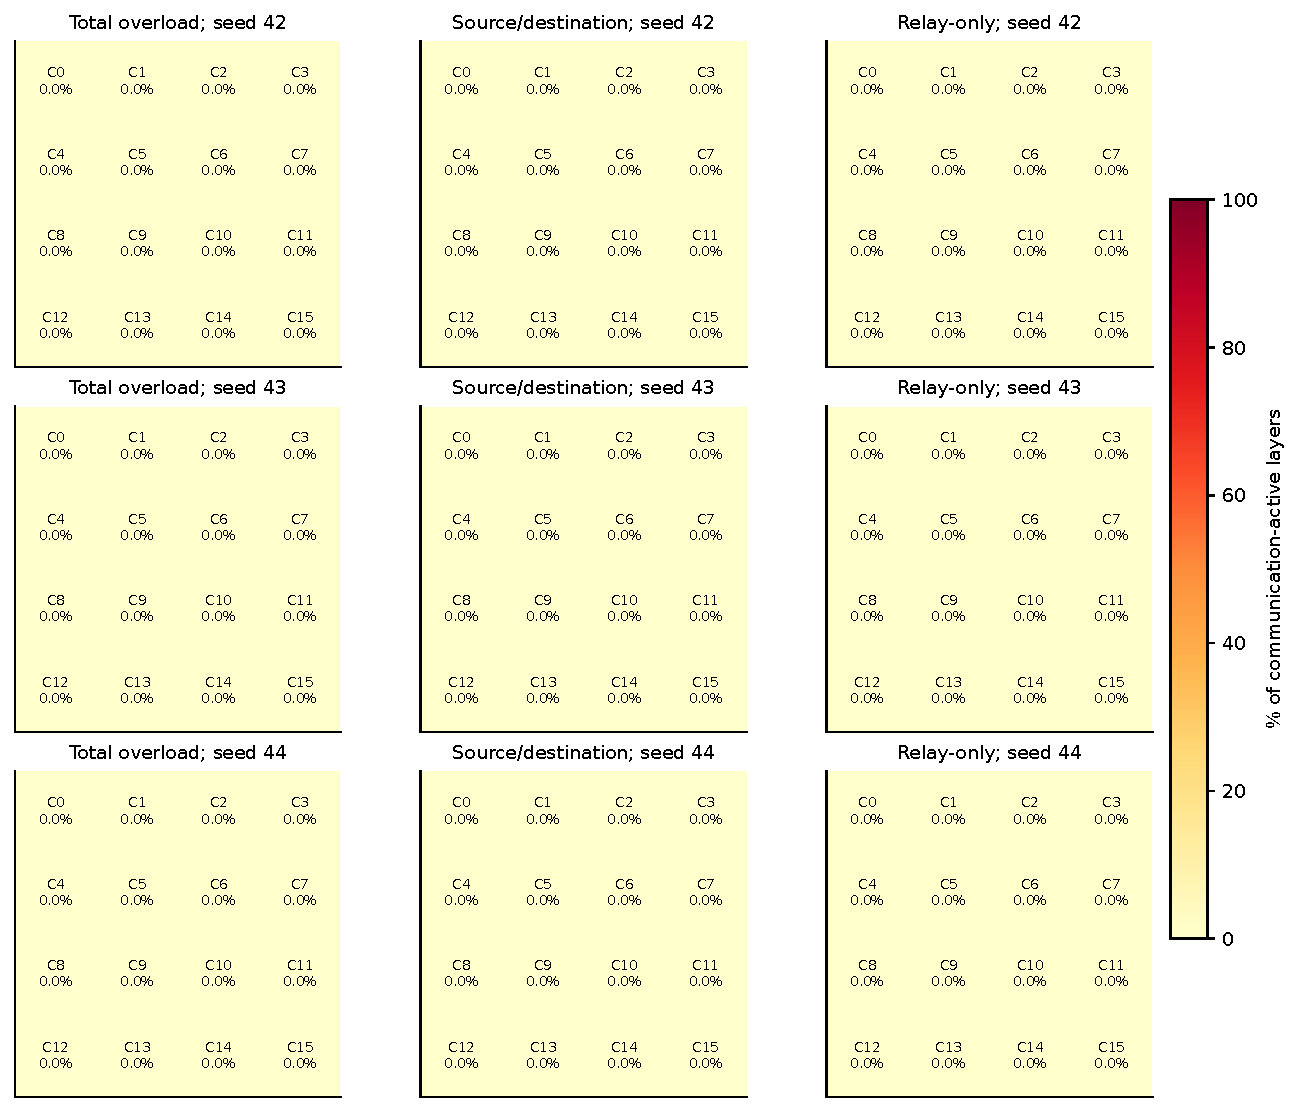
\includegraphics[width=.94\linewidth,height=.48\textheight,keepaspectratio]{figures/atlas/mesh_yx_route_m32.pdf}\captionof{figure}{All three conceptual mapping seeds; common 0--100 percent colour scale.}\end{center}
\begin{center}{\scriptsize\setlength{\tabcolsep}{3pt}
\begin{tabular}{lrrrrrrrrr}
\toprule
Core & 42 Tot & 42 Own & 42 Rel & 43 Tot & 43 Own & 43 Rel & 44 Tot & 44 Own & 44 Rel \\
\midrule
0 & 0.000 & 0.000 & 0.000 & 0.000 & 0.000 & 0.000 & 0.000 & 0.000 & 0.000 \\
1 & 0.000 & 0.000 & 0.000 & 0.000 & 0.000 & 0.000 & 0.000 & 0.000 & 0.000 \\
2 & 0.000 & 0.000 & 0.000 & 0.000 & 0.000 & 0.000 & 0.000 & 0.000 & 0.000 \\
3 & 0.000 & 0.000 & 0.000 & 0.000 & 0.000 & 0.000 & 0.000 & 0.000 & 0.000 \\
4 & 0.000 & 0.000 & 0.000 & 0.000 & 0.000 & 0.000 & 0.000 & 0.000 & 0.000 \\
5 & 0.000 & 0.000 & 0.000 & 0.000 & 0.000 & 0.000 & 0.000 & 0.000 & 0.000 \\
6 & 0.000 & 0.000 & 0.000 & 0.000 & 0.000 & 0.000 & 0.000 & 0.000 & 0.000 \\
7 & 0.000 & 0.000 & 0.000 & 0.000 & 0.000 & 0.000 & 0.000 & 0.000 & 0.000 \\
8 & 0.000 & 0.000 & 0.000 & 0.000 & 0.000 & 0.000 & 0.000 & 0.000 & 0.000 \\
9 & 0.000 & 0.000 & 0.000 & 0.000 & 0.000 & 0.000 & 0.000 & 0.000 & 0.000 \\
10 & 0.000 & 0.000 & 0.000 & 0.000 & 0.000 & 0.000 & 0.000 & 0.000 & 0.000 \\
11 & 0.000 & 0.000 & 0.000 & 0.000 & 0.000 & 0.000 & 0.000 & 0.000 & 0.000 \\
12 & 0.000 & 0.000 & 0.000 & 0.000 & 0.000 & 0.000 & 0.000 & 0.000 & 0.000 \\
13 & 0.000 & 0.000 & 0.000 & 0.000 & 0.000 & 0.000 & 0.000 & 0.000 & 0.000 \\
14 & 0.000 & 0.000 & 0.000 & 0.000 & 0.000 & 0.000 & 0.000 & 0.000 & 0.000 \\
15 & 0.000 & 0.000 & 0.000 & 0.000 & 0.000 & 0.000 & 0.000 & 0.000 & 0.000 \\
\bottomrule\end{tabular}}
\captionof{table}{Exact heatmap percentages, with Tot = Own + Rel. Unrounded values are in the CSV.}
{\footnotesize\href{https://github.com/sanjeevkrishnaa/Compiler-Driven-ACE/blob/codex/ace-scheduler-correctness/docs/latex/qft96_final/data/heatmap_mesh_yx_route_m32.csv}{Exact CSV values and sample counts}}
\end{center}
\clearpage\subsection*{Mesh yx; M=2; hop counting}
\begin{center}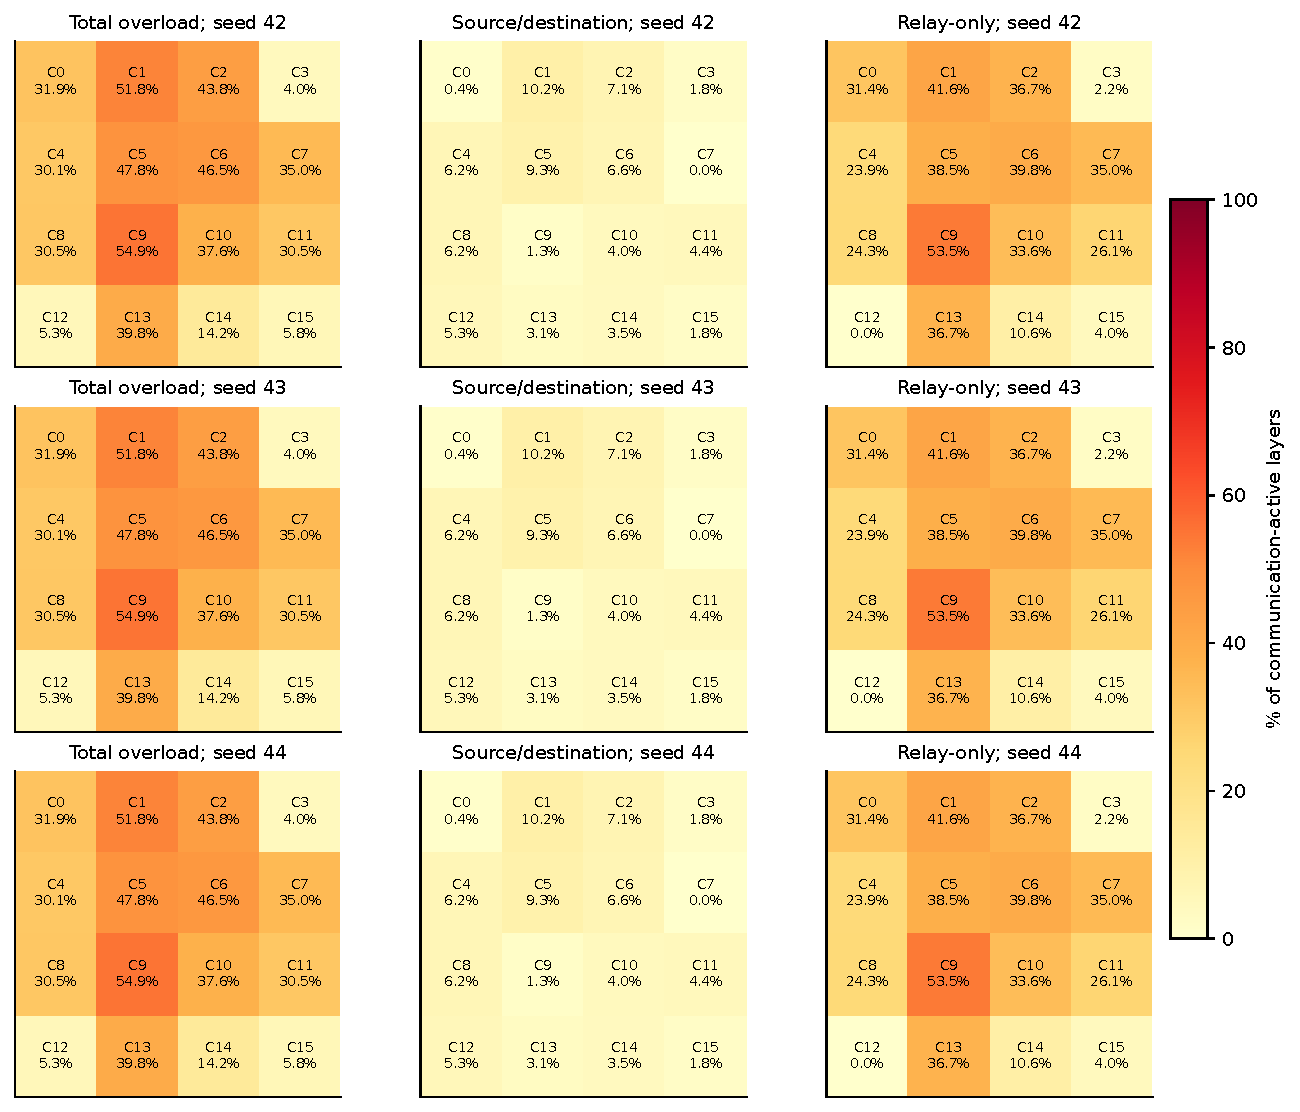
\includegraphics[width=.94\linewidth,height=.48\textheight,keepaspectratio]{figures/atlas/mesh_yx_hop_m2.pdf}\captionof{figure}{All three conceptual mapping seeds; common 0--100 percent colour scale.}\end{center}
\begin{center}{\scriptsize\setlength{\tabcolsep}{3pt}
\begin{tabular}{lrrrrrrrrr}
\toprule
Core & 42 Tot & 42 Own & 42 Rel & 43 Tot & 43 Own & 43 Rel & 44 Tot & 44 Own & 44 Rel \\
\midrule
0 & 31.858 & 0.442 & 31.416 & 31.858 & 0.442 & 31.416 & 31.858 & 0.442 & 31.416 \\
1 & 51.770 & 10.177 & 41.593 & 51.770 & 10.177 & 41.593 & 51.770 & 10.177 & 41.593 \\
2 & 43.805 & 7.080 & 36.726 & 43.805 & 7.080 & 36.726 & 43.805 & 7.080 & 36.726 \\
3 & 3.982 & 1.770 & 2.212 & 3.982 & 1.770 & 2.212 & 3.982 & 1.770 & 2.212 \\
4 & 30.088 & 6.195 & 23.894 & 30.088 & 6.195 & 23.894 & 30.088 & 6.195 & 23.894 \\
5 & 47.788 & 9.292 & 38.496 & 47.788 & 9.292 & 38.496 & 47.788 & 9.292 & 38.496 \\
6 & 46.460 & 6.637 & 39.823 & 46.460 & 6.637 & 39.823 & 46.460 & 6.637 & 39.823 \\
7 & 34.956 & 0.000 & 34.956 & 34.956 & 0.000 & 34.956 & 34.956 & 0.000 & 34.956 \\
8 & 30.531 & 6.195 & 24.336 & 30.531 & 6.195 & 24.336 & 30.531 & 6.195 & 24.336 \\
9 & 54.867 & 1.327 & 53.540 & 54.867 & 1.327 & 53.540 & 54.867 & 1.327 & 53.540 \\
10 & 37.611 & 3.982 & 33.628 & 37.611 & 3.982 & 33.628 & 37.611 & 3.982 & 33.628 \\
11 & 30.531 & 4.425 & 26.106 & 30.531 & 4.425 & 26.106 & 30.531 & 4.425 & 26.106 \\
12 & 5.310 & 5.310 & 0.000 & 5.310 & 5.310 & 0.000 & 5.310 & 5.310 & 0.000 \\
13 & 39.823 & 3.097 & 36.726 & 39.823 & 3.097 & 36.726 & 39.823 & 3.097 & 36.726 \\
14 & 14.159 & 3.540 & 10.619 & 14.159 & 3.540 & 10.619 & 14.159 & 3.540 & 10.619 \\
15 & 5.752 & 1.770 & 3.982 & 5.752 & 1.770 & 3.982 & 5.752 & 1.770 & 3.982 \\
\bottomrule\end{tabular}}
\captionof{table}{Exact heatmap percentages, with Tot = Own + Rel. Unrounded values are in the CSV.}
{\footnotesize\href{https://github.com/sanjeevkrishnaa/Compiler-Driven-ACE/blob/codex/ace-scheduler-correctness/docs/latex/qft96_final/data/heatmap_mesh_yx_hop_m2.csv}{Exact CSV values and sample counts}}
\end{center}
\clearpage\subsection*{Mesh yx; M=3; hop counting}
\begin{center}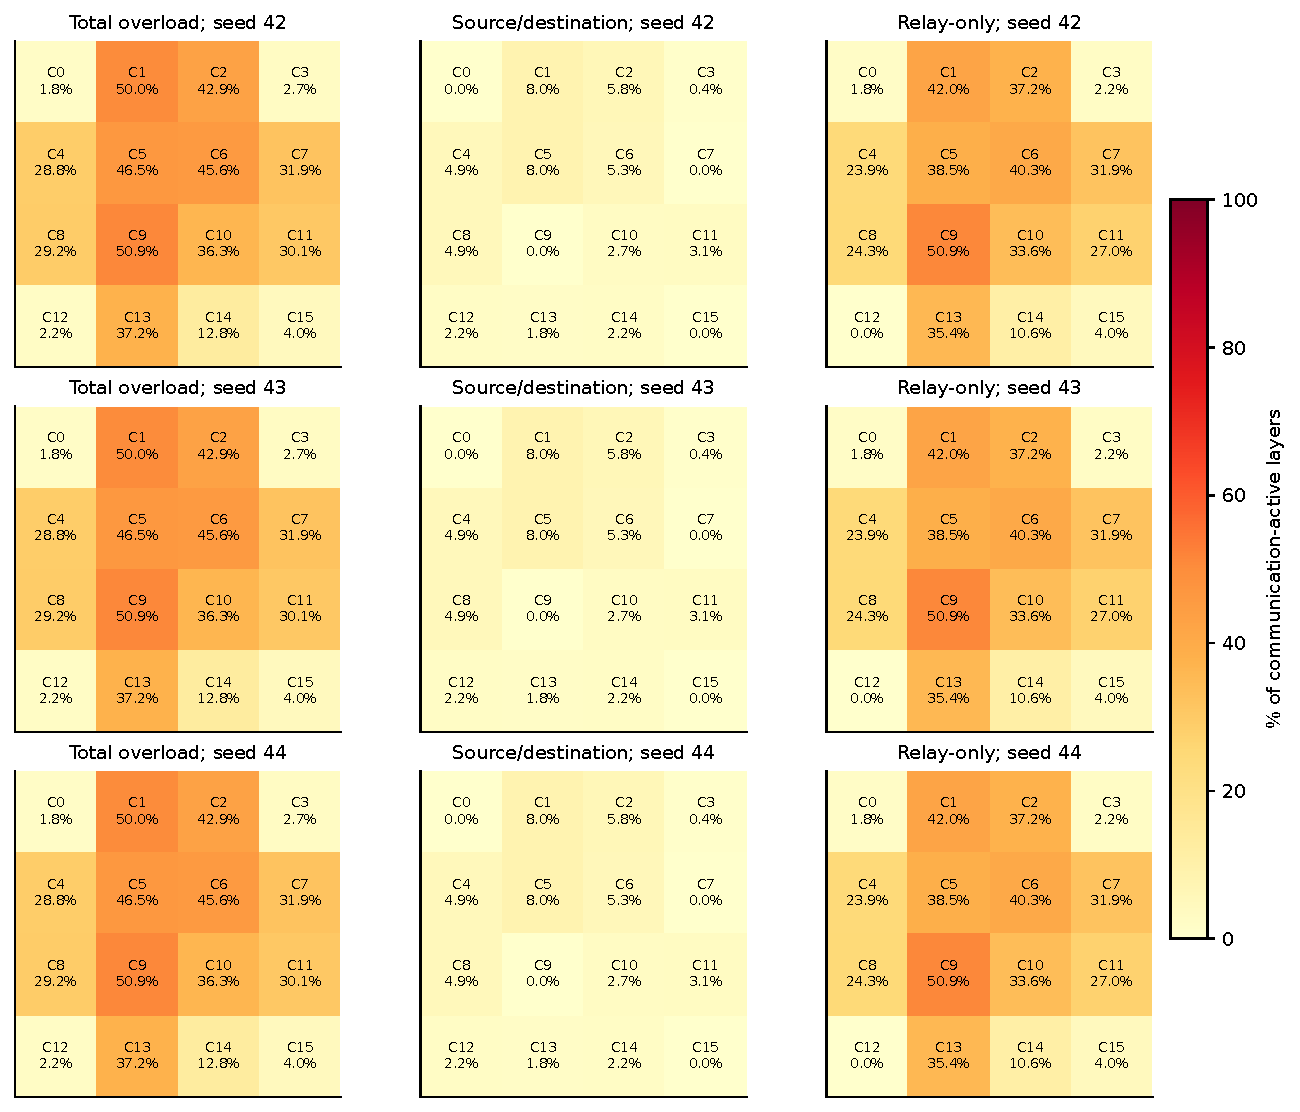
\includegraphics[width=.94\linewidth,height=.48\textheight,keepaspectratio]{figures/atlas/mesh_yx_hop_m3.pdf}\captionof{figure}{All three conceptual mapping seeds; common 0--100 percent colour scale.}\end{center}
\begin{center}{\scriptsize\setlength{\tabcolsep}{3pt}
\begin{tabular}{lrrrrrrrrr}
\toprule
Core & 42 Tot & 42 Own & 42 Rel & 43 Tot & 43 Own & 43 Rel & 44 Tot & 44 Own & 44 Rel \\
\midrule
0 & 1.770 & 0.000 & 1.770 & 1.770 & 0.000 & 1.770 & 1.770 & 0.000 & 1.770 \\
1 & 50.000 & 7.965 & 42.035 & 50.000 & 7.965 & 42.035 & 50.000 & 7.965 & 42.035 \\
2 & 42.920 & 5.752 & 37.168 & 42.920 & 5.752 & 37.168 & 42.920 & 5.752 & 37.168 \\
3 & 2.655 & 0.442 & 2.212 & 2.655 & 0.442 & 2.212 & 2.655 & 0.442 & 2.212 \\
4 & 28.761 & 4.867 & 23.894 & 28.761 & 4.867 & 23.894 & 28.761 & 4.867 & 23.894 \\
5 & 46.460 & 7.965 & 38.496 & 46.460 & 7.965 & 38.496 & 46.460 & 7.965 & 38.496 \\
6 & 45.575 & 5.310 & 40.265 & 45.575 & 5.310 & 40.265 & 45.575 & 5.310 & 40.265 \\
7 & 31.858 & 0.000 & 31.858 & 31.858 & 0.000 & 31.858 & 31.858 & 0.000 & 31.858 \\
8 & 29.204 & 4.867 & 24.336 & 29.204 & 4.867 & 24.336 & 29.204 & 4.867 & 24.336 \\
9 & 50.885 & 0.000 & 50.885 & 50.885 & 0.000 & 50.885 & 50.885 & 0.000 & 50.885 \\
10 & 36.283 & 2.655 & 33.628 & 36.283 & 2.655 & 33.628 & 36.283 & 2.655 & 33.628 \\
11 & 30.088 & 3.097 & 26.991 & 30.088 & 3.097 & 26.991 & 30.088 & 3.097 & 26.991 \\
12 & 2.212 & 2.212 & 0.000 & 2.212 & 2.212 & 0.000 & 2.212 & 2.212 & 0.000 \\
13 & 37.168 & 1.770 & 35.398 & 37.168 & 1.770 & 35.398 & 37.168 & 1.770 & 35.398 \\
14 & 12.832 & 2.212 & 10.619 & 12.832 & 2.212 & 10.619 & 12.832 & 2.212 & 10.619 \\
15 & 3.982 & 0.000 & 3.982 & 3.982 & 0.000 & 3.982 & 3.982 & 0.000 & 3.982 \\
\bottomrule\end{tabular}}
\captionof{table}{Exact heatmap percentages, with Tot = Own + Rel. Unrounded values are in the CSV.}
{\footnotesize\href{https://github.com/sanjeevkrishnaa/Compiler-Driven-ACE/blob/codex/ace-scheduler-correctness/docs/latex/qft96_final/data/heatmap_mesh_yx_hop_m3.csv}{Exact CSV values and sample counts}}
\end{center}
\clearpage\subsection*{Mesh yx; M=4; hop counting}
\begin{center}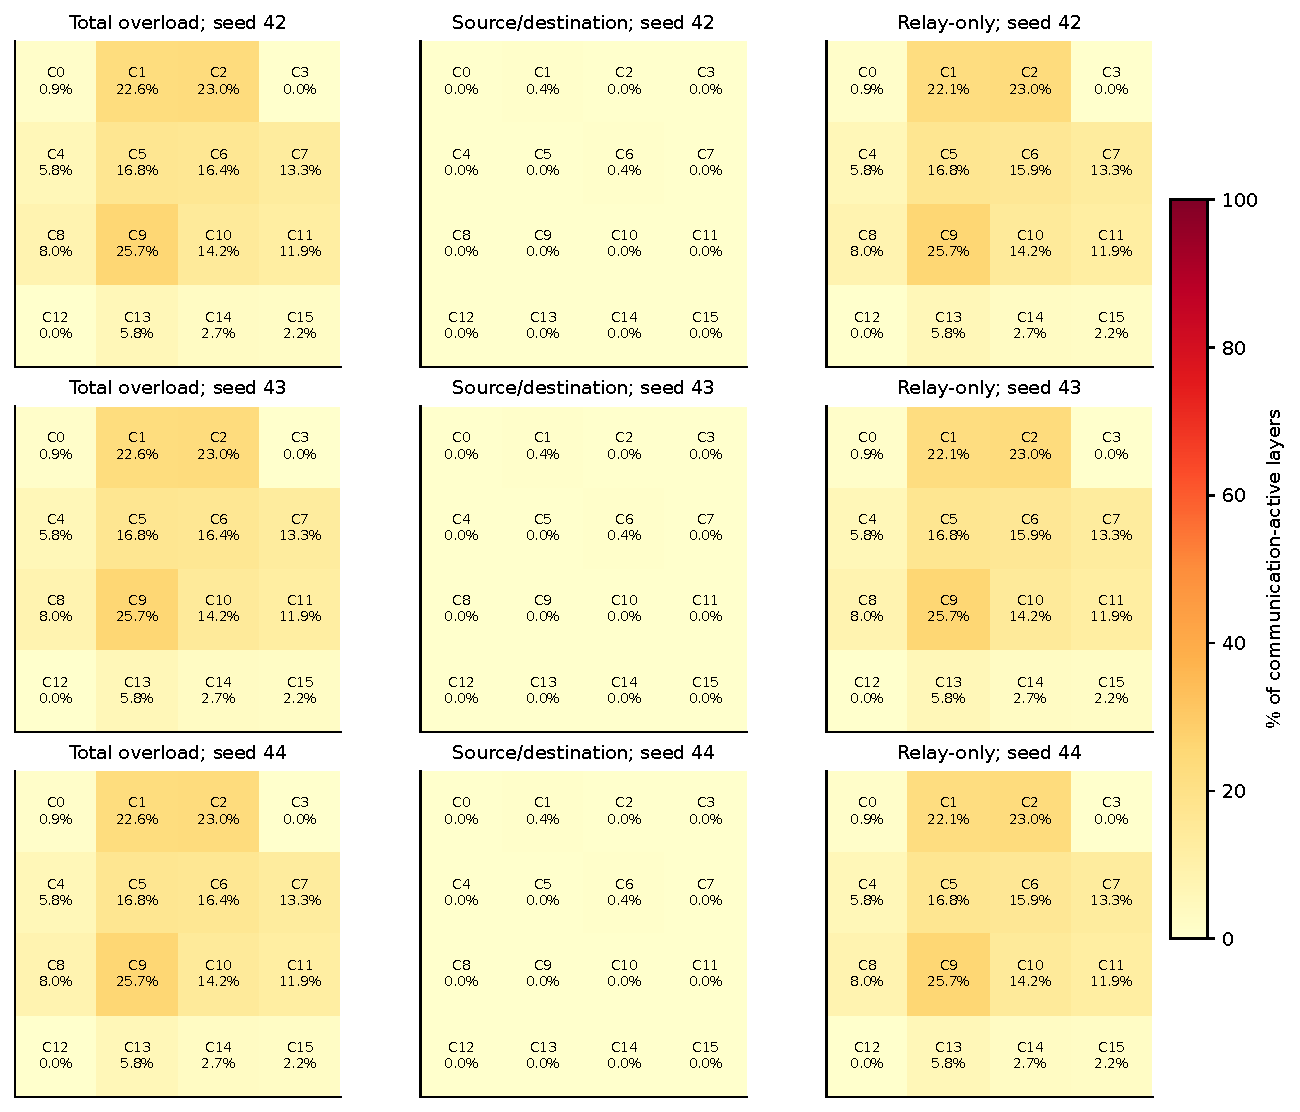
\includegraphics[width=.94\linewidth,height=.48\textheight,keepaspectratio]{figures/atlas/mesh_yx_hop_m4.pdf}\captionof{figure}{All three conceptual mapping seeds; common 0--100 percent colour scale.}\end{center}
\begin{center}{\scriptsize\setlength{\tabcolsep}{3pt}
\begin{tabular}{lrrrrrrrrr}
\toprule
Core & 42 Tot & 42 Own & 42 Rel & 43 Tot & 43 Own & 43 Rel & 44 Tot & 44 Own & 44 Rel \\
\midrule
0 & 0.885 & 0.000 & 0.885 & 0.885 & 0.000 & 0.885 & 0.885 & 0.000 & 0.885 \\
1 & 22.566 & 0.442 & 22.124 & 22.566 & 0.442 & 22.124 & 22.566 & 0.442 & 22.124 \\
2 & 23.009 & 0.000 & 23.009 & 23.009 & 0.000 & 23.009 & 23.009 & 0.000 & 23.009 \\
3 & 0.000 & 0.000 & 0.000 & 0.000 & 0.000 & 0.000 & 0.000 & 0.000 & 0.000 \\
4 & 5.752 & 0.000 & 5.752 & 5.752 & 0.000 & 5.752 & 5.752 & 0.000 & 5.752 \\
5 & 16.814 & 0.000 & 16.814 & 16.814 & 0.000 & 16.814 & 16.814 & 0.000 & 16.814 \\
6 & 16.372 & 0.442 & 15.929 & 16.372 & 0.442 & 15.929 & 16.372 & 0.442 & 15.929 \\
7 & 13.274 & 0.000 & 13.274 & 13.274 & 0.000 & 13.274 & 13.274 & 0.000 & 13.274 \\
8 & 7.965 & 0.000 & 7.965 & 7.965 & 0.000 & 7.965 & 7.965 & 0.000 & 7.965 \\
9 & 25.664 & 0.000 & 25.664 & 25.664 & 0.000 & 25.664 & 25.664 & 0.000 & 25.664 \\
10 & 14.159 & 0.000 & 14.159 & 14.159 & 0.000 & 14.159 & 14.159 & 0.000 & 14.159 \\
11 & 11.947 & 0.000 & 11.947 & 11.947 & 0.000 & 11.947 & 11.947 & 0.000 & 11.947 \\
12 & 0.000 & 0.000 & 0.000 & 0.000 & 0.000 & 0.000 & 0.000 & 0.000 & 0.000 \\
13 & 5.752 & 0.000 & 5.752 & 5.752 & 0.000 & 5.752 & 5.752 & 0.000 & 5.752 \\
14 & 2.655 & 0.000 & 2.655 & 2.655 & 0.000 & 2.655 & 2.655 & 0.000 & 2.655 \\
15 & 2.212 & 0.000 & 2.212 & 2.212 & 0.000 & 2.212 & 2.212 & 0.000 & 2.212 \\
\bottomrule\end{tabular}}
\captionof{table}{Exact heatmap percentages, with Tot = Own + Rel. Unrounded values are in the CSV.}
{\footnotesize\href{https://github.com/sanjeevkrishnaa/Compiler-Driven-ACE/blob/codex/ace-scheduler-correctness/docs/latex/qft96_final/data/heatmap_mesh_yx_hop_m4.csv}{Exact CSV values and sample counts}}
\end{center}
\clearpage\subsection*{Mesh yx; M=6; hop counting}
\begin{center}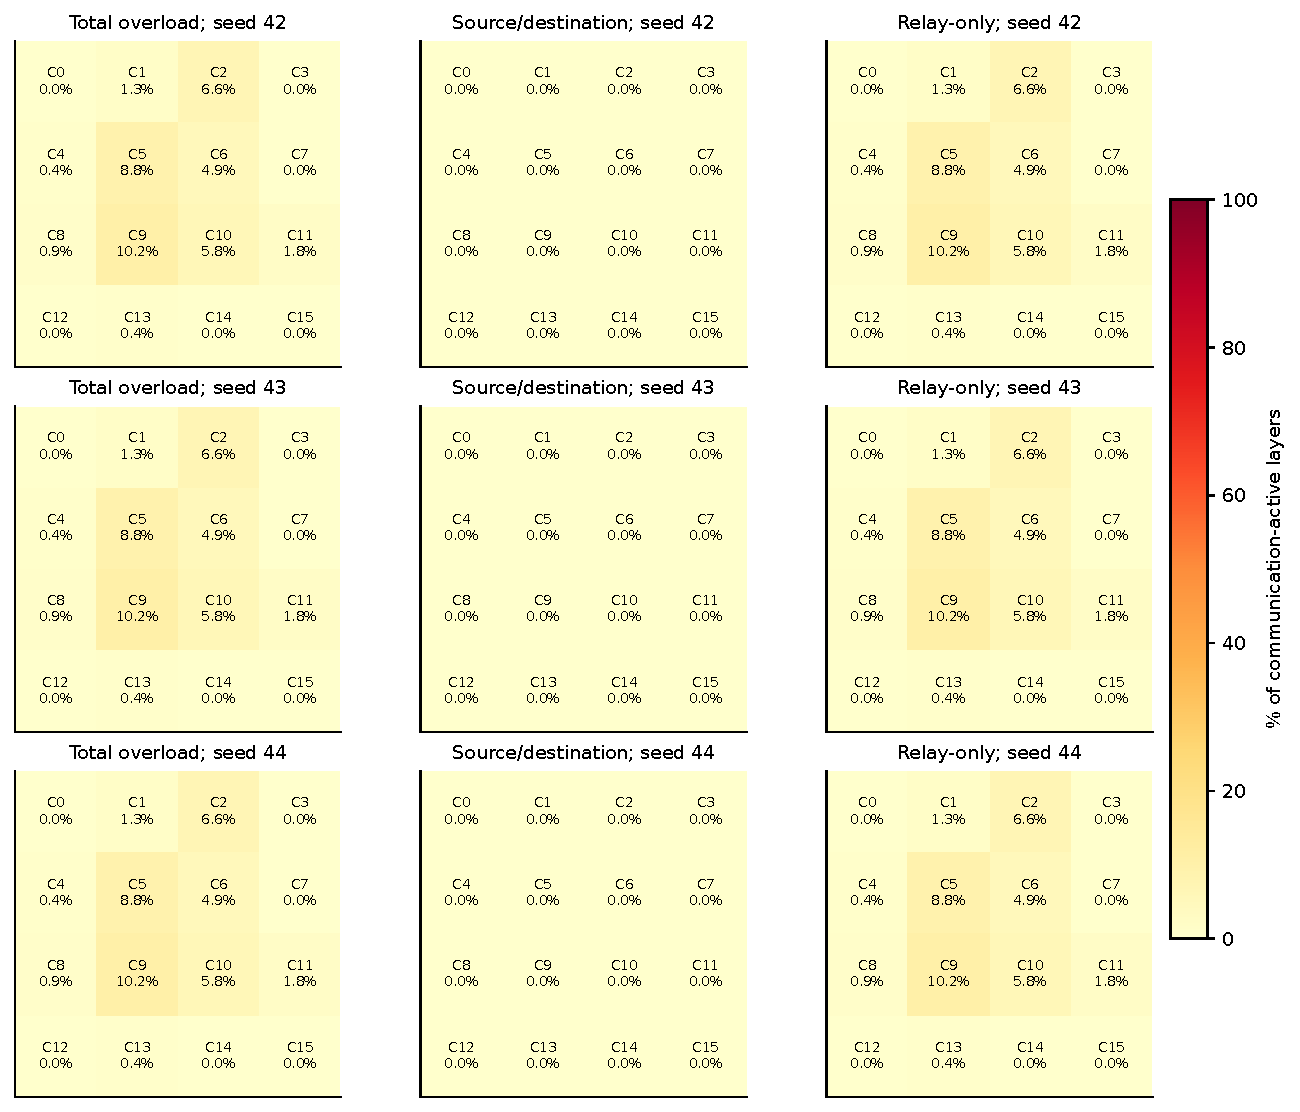
\includegraphics[width=.94\linewidth,height=.48\textheight,keepaspectratio]{figures/atlas/mesh_yx_hop_m6.pdf}\captionof{figure}{All three conceptual mapping seeds; common 0--100 percent colour scale.}\end{center}
\begin{center}{\scriptsize\setlength{\tabcolsep}{3pt}
\begin{tabular}{lrrrrrrrrr}
\toprule
Core & 42 Tot & 42 Own & 42 Rel & 43 Tot & 43 Own & 43 Rel & 44 Tot & 44 Own & 44 Rel \\
\midrule
0 & 0.000 & 0.000 & 0.000 & 0.000 & 0.000 & 0.000 & 0.000 & 0.000 & 0.000 \\
1 & 1.327 & 0.000 & 1.327 & 1.327 & 0.000 & 1.327 & 1.327 & 0.000 & 1.327 \\
2 & 6.637 & 0.000 & 6.637 & 6.637 & 0.000 & 6.637 & 6.637 & 0.000 & 6.637 \\
3 & 0.000 & 0.000 & 0.000 & 0.000 & 0.000 & 0.000 & 0.000 & 0.000 & 0.000 \\
4 & 0.442 & 0.000 & 0.442 & 0.442 & 0.000 & 0.442 & 0.442 & 0.000 & 0.442 \\
5 & 8.850 & 0.000 & 8.850 & 8.850 & 0.000 & 8.850 & 8.850 & 0.000 & 8.850 \\
6 & 4.867 & 0.000 & 4.867 & 4.867 & 0.000 & 4.867 & 4.867 & 0.000 & 4.867 \\
7 & 0.000 & 0.000 & 0.000 & 0.000 & 0.000 & 0.000 & 0.000 & 0.000 & 0.000 \\
8 & 0.885 & 0.000 & 0.885 & 0.885 & 0.000 & 0.885 & 0.885 & 0.000 & 0.885 \\
9 & 10.177 & 0.000 & 10.177 & 10.177 & 0.000 & 10.177 & 10.177 & 0.000 & 10.177 \\
10 & 5.752 & 0.000 & 5.752 & 5.752 & 0.000 & 5.752 & 5.752 & 0.000 & 5.752 \\
11 & 1.770 & 0.000 & 1.770 & 1.770 & 0.000 & 1.770 & 1.770 & 0.000 & 1.770 \\
12 & 0.000 & 0.000 & 0.000 & 0.000 & 0.000 & 0.000 & 0.000 & 0.000 & 0.000 \\
13 & 0.442 & 0.000 & 0.442 & 0.442 & 0.000 & 0.442 & 0.442 & 0.000 & 0.442 \\
14 & 0.000 & 0.000 & 0.000 & 0.000 & 0.000 & 0.000 & 0.000 & 0.000 & 0.000 \\
15 & 0.000 & 0.000 & 0.000 & 0.000 & 0.000 & 0.000 & 0.000 & 0.000 & 0.000 \\
\bottomrule\end{tabular}}
\captionof{table}{Exact heatmap percentages, with Tot = Own + Rel. Unrounded values are in the CSV.}
{\footnotesize\href{https://github.com/sanjeevkrishnaa/Compiler-Driven-ACE/blob/codex/ace-scheduler-correctness/docs/latex/qft96_final/data/heatmap_mesh_yx_hop_m6.csv}{Exact CSV values and sample counts}}
\end{center}
\clearpage\subsection*{Mesh yx; M=8; hop counting}
\begin{center}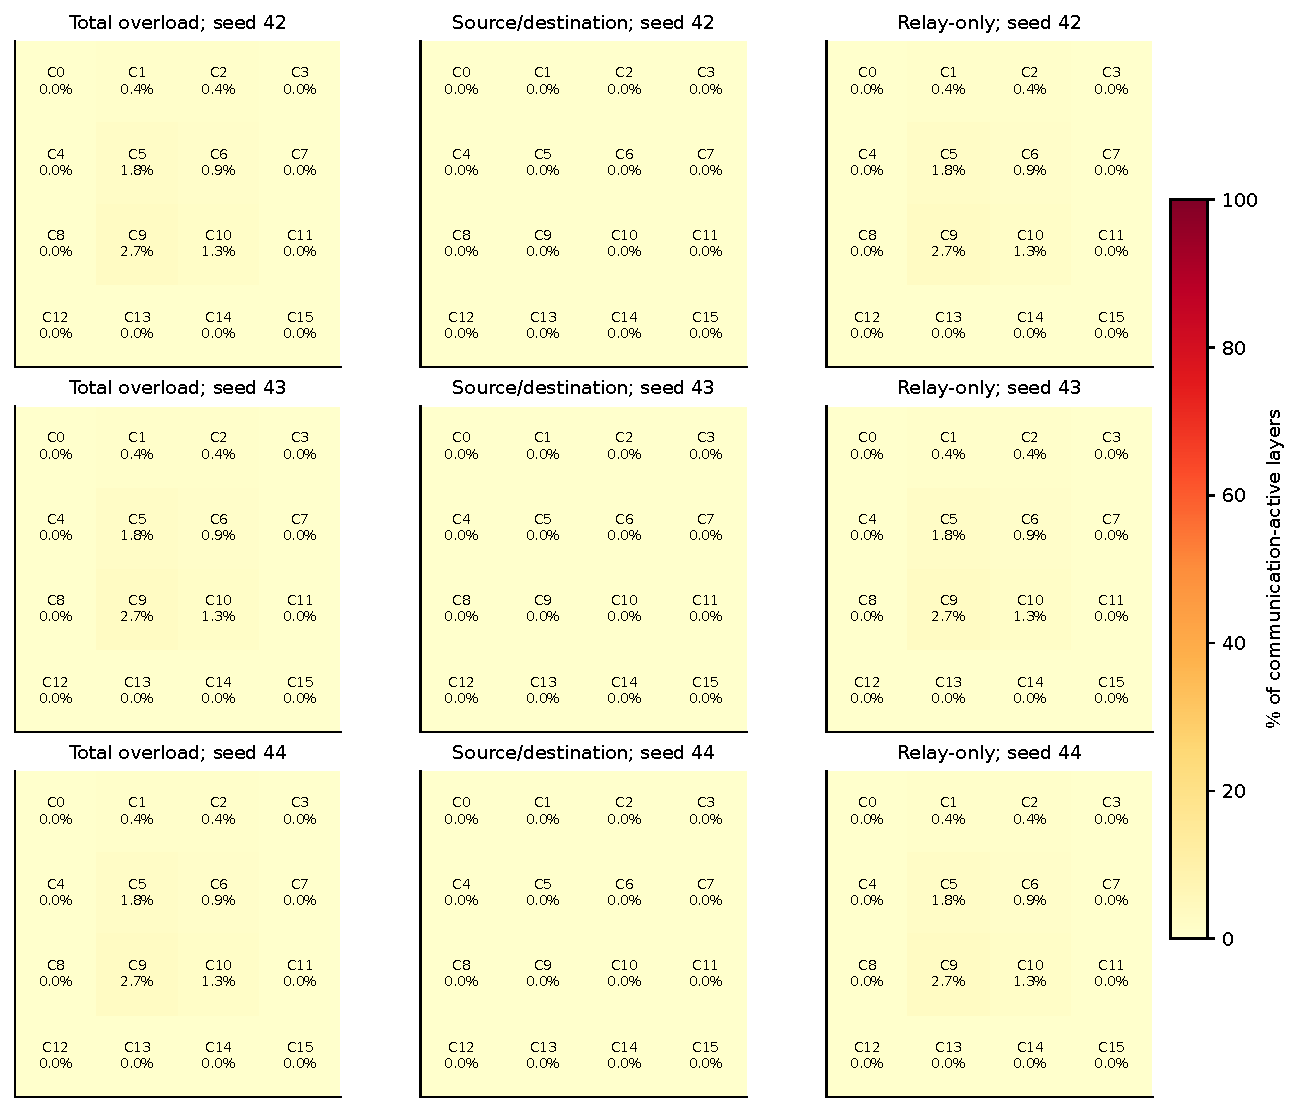
\includegraphics[width=.94\linewidth,height=.48\textheight,keepaspectratio]{figures/atlas/mesh_yx_hop_m8.pdf}\captionof{figure}{All three conceptual mapping seeds; common 0--100 percent colour scale.}\end{center}
\begin{center}{\scriptsize\setlength{\tabcolsep}{3pt}
\begin{tabular}{lrrrrrrrrr}
\toprule
Core & 42 Tot & 42 Own & 42 Rel & 43 Tot & 43 Own & 43 Rel & 44 Tot & 44 Own & 44 Rel \\
\midrule
0 & 0.000 & 0.000 & 0.000 & 0.000 & 0.000 & 0.000 & 0.000 & 0.000 & 0.000 \\
1 & 0.442 & 0.000 & 0.442 & 0.442 & 0.000 & 0.442 & 0.442 & 0.000 & 0.442 \\
2 & 0.442 & 0.000 & 0.442 & 0.442 & 0.000 & 0.442 & 0.442 & 0.000 & 0.442 \\
3 & 0.000 & 0.000 & 0.000 & 0.000 & 0.000 & 0.000 & 0.000 & 0.000 & 0.000 \\
4 & 0.000 & 0.000 & 0.000 & 0.000 & 0.000 & 0.000 & 0.000 & 0.000 & 0.000 \\
5 & 1.770 & 0.000 & 1.770 & 1.770 & 0.000 & 1.770 & 1.770 & 0.000 & 1.770 \\
6 & 0.885 & 0.000 & 0.885 & 0.885 & 0.000 & 0.885 & 0.885 & 0.000 & 0.885 \\
7 & 0.000 & 0.000 & 0.000 & 0.000 & 0.000 & 0.000 & 0.000 & 0.000 & 0.000 \\
8 & 0.000 & 0.000 & 0.000 & 0.000 & 0.000 & 0.000 & 0.000 & 0.000 & 0.000 \\
9 & 2.655 & 0.000 & 2.655 & 2.655 & 0.000 & 2.655 & 2.655 & 0.000 & 2.655 \\
10 & 1.327 & 0.000 & 1.327 & 1.327 & 0.000 & 1.327 & 1.327 & 0.000 & 1.327 \\
11 & 0.000 & 0.000 & 0.000 & 0.000 & 0.000 & 0.000 & 0.000 & 0.000 & 0.000 \\
12 & 0.000 & 0.000 & 0.000 & 0.000 & 0.000 & 0.000 & 0.000 & 0.000 & 0.000 \\
13 & 0.000 & 0.000 & 0.000 & 0.000 & 0.000 & 0.000 & 0.000 & 0.000 & 0.000 \\
14 & 0.000 & 0.000 & 0.000 & 0.000 & 0.000 & 0.000 & 0.000 & 0.000 & 0.000 \\
15 & 0.000 & 0.000 & 0.000 & 0.000 & 0.000 & 0.000 & 0.000 & 0.000 & 0.000 \\
\bottomrule\end{tabular}}
\captionof{table}{Exact heatmap percentages, with Tot = Own + Rel. Unrounded values are in the CSV.}
{\footnotesize\href{https://github.com/sanjeevkrishnaa/Compiler-Driven-ACE/blob/codex/ace-scheduler-correctness/docs/latex/qft96_final/data/heatmap_mesh_yx_hop_m8.csv}{Exact CSV values and sample counts}}
\end{center}
\clearpage\subsection*{Mesh yx; M=16; hop counting}
\begin{center}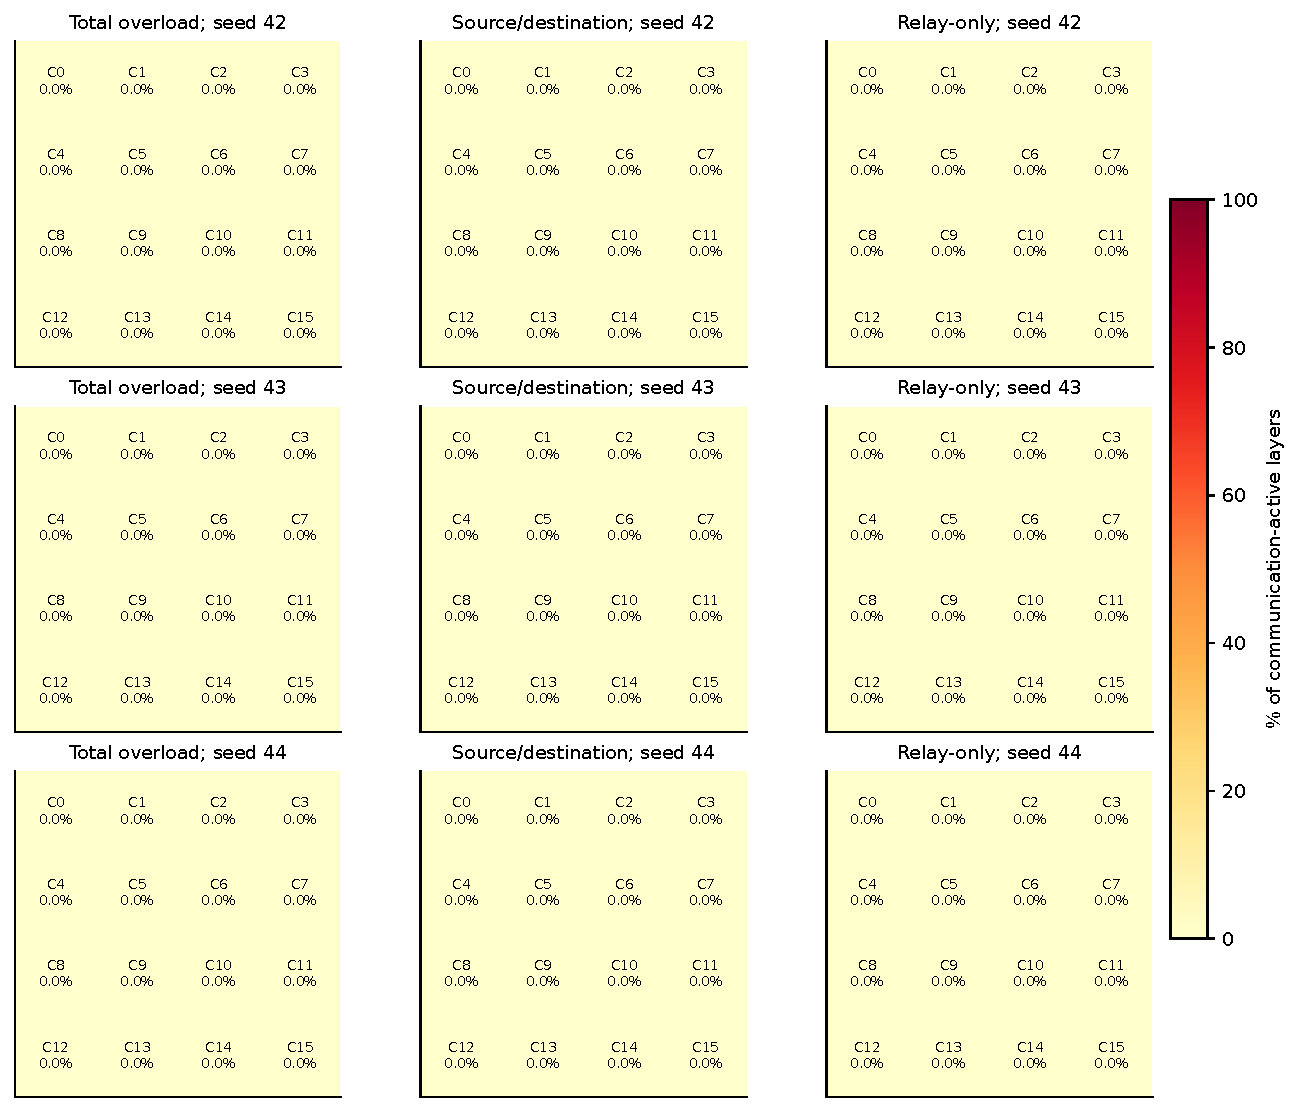
\includegraphics[width=.94\linewidth,height=.48\textheight,keepaspectratio]{figures/atlas/mesh_yx_hop_m16.pdf}\captionof{figure}{All three conceptual mapping seeds; common 0--100 percent colour scale.}\end{center}
\begin{center}{\scriptsize\setlength{\tabcolsep}{3pt}
\begin{tabular}{lrrrrrrrrr}
\toprule
Core & 42 Tot & 42 Own & 42 Rel & 43 Tot & 43 Own & 43 Rel & 44 Tot & 44 Own & 44 Rel \\
\midrule
0 & 0.000 & 0.000 & 0.000 & 0.000 & 0.000 & 0.000 & 0.000 & 0.000 & 0.000 \\
1 & 0.000 & 0.000 & 0.000 & 0.000 & 0.000 & 0.000 & 0.000 & 0.000 & 0.000 \\
2 & 0.000 & 0.000 & 0.000 & 0.000 & 0.000 & 0.000 & 0.000 & 0.000 & 0.000 \\
3 & 0.000 & 0.000 & 0.000 & 0.000 & 0.000 & 0.000 & 0.000 & 0.000 & 0.000 \\
4 & 0.000 & 0.000 & 0.000 & 0.000 & 0.000 & 0.000 & 0.000 & 0.000 & 0.000 \\
5 & 0.000 & 0.000 & 0.000 & 0.000 & 0.000 & 0.000 & 0.000 & 0.000 & 0.000 \\
6 & 0.000 & 0.000 & 0.000 & 0.000 & 0.000 & 0.000 & 0.000 & 0.000 & 0.000 \\
7 & 0.000 & 0.000 & 0.000 & 0.000 & 0.000 & 0.000 & 0.000 & 0.000 & 0.000 \\
8 & 0.000 & 0.000 & 0.000 & 0.000 & 0.000 & 0.000 & 0.000 & 0.000 & 0.000 \\
9 & 0.000 & 0.000 & 0.000 & 0.000 & 0.000 & 0.000 & 0.000 & 0.000 & 0.000 \\
10 & 0.000 & 0.000 & 0.000 & 0.000 & 0.000 & 0.000 & 0.000 & 0.000 & 0.000 \\
11 & 0.000 & 0.000 & 0.000 & 0.000 & 0.000 & 0.000 & 0.000 & 0.000 & 0.000 \\
12 & 0.000 & 0.000 & 0.000 & 0.000 & 0.000 & 0.000 & 0.000 & 0.000 & 0.000 \\
13 & 0.000 & 0.000 & 0.000 & 0.000 & 0.000 & 0.000 & 0.000 & 0.000 & 0.000 \\
14 & 0.000 & 0.000 & 0.000 & 0.000 & 0.000 & 0.000 & 0.000 & 0.000 & 0.000 \\
15 & 0.000 & 0.000 & 0.000 & 0.000 & 0.000 & 0.000 & 0.000 & 0.000 & 0.000 \\
\bottomrule\end{tabular}}
\captionof{table}{Exact heatmap percentages, with Tot = Own + Rel. Unrounded values are in the CSV.}
{\footnotesize\href{https://github.com/sanjeevkrishnaa/Compiler-Driven-ACE/blob/codex/ace-scheduler-correctness/docs/latex/qft96_final/data/heatmap_mesh_yx_hop_m16.csv}{Exact CSV values and sample counts}}
\end{center}
\clearpage\subsection*{Mesh yx; M=32; hop counting}
\begin{center}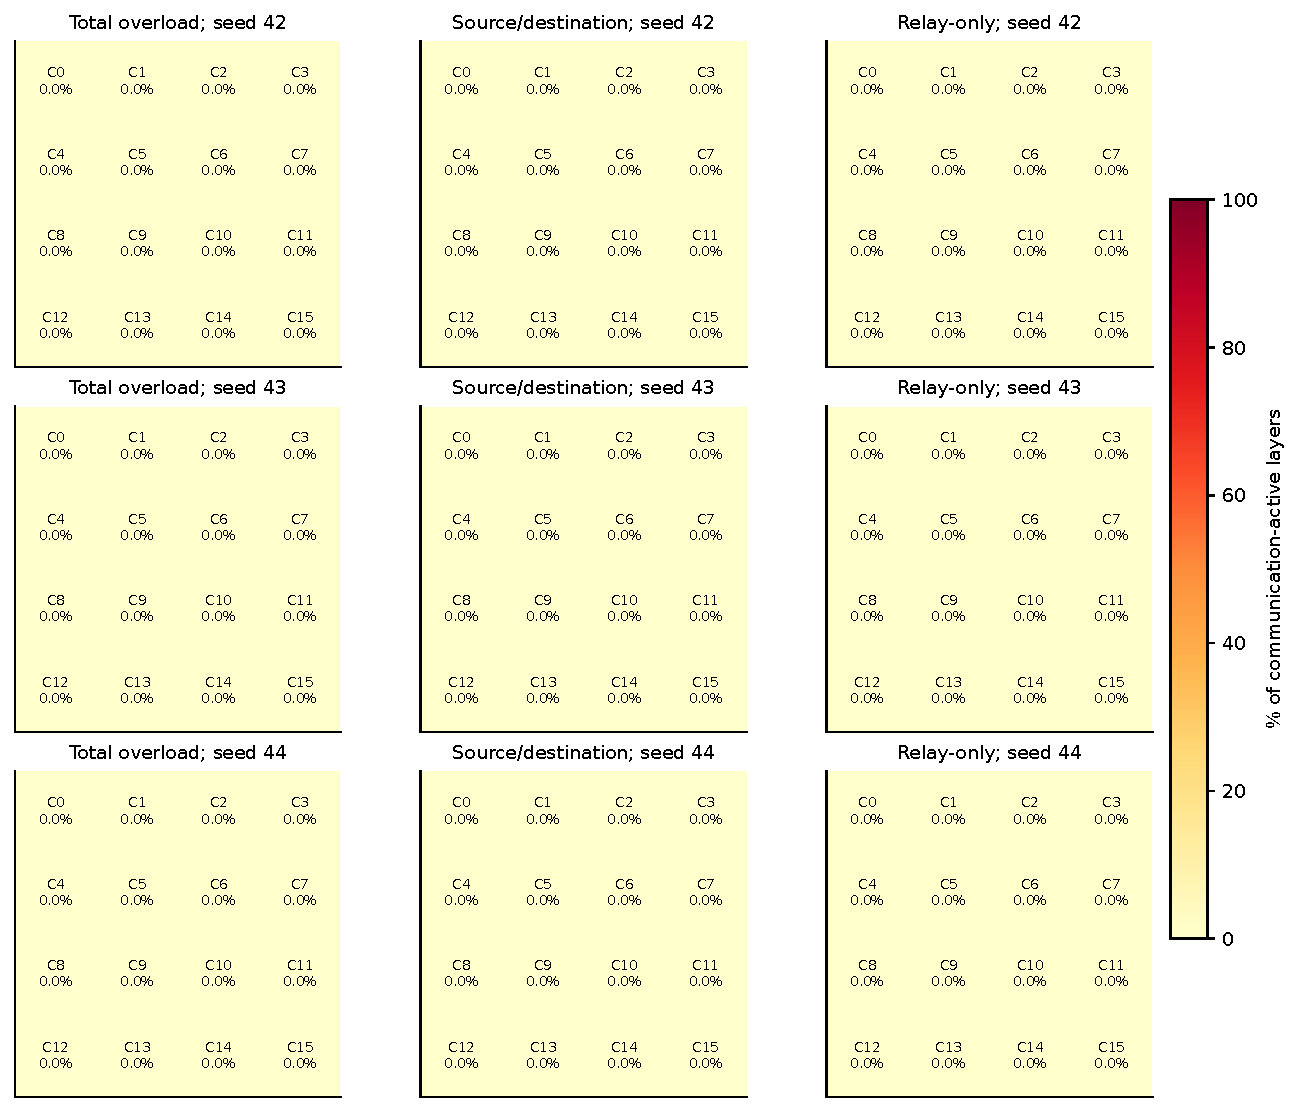
\includegraphics[width=.94\linewidth,height=.48\textheight,keepaspectratio]{figures/atlas/mesh_yx_hop_m32.pdf}\captionof{figure}{All three conceptual mapping seeds; common 0--100 percent colour scale.}\end{center}
\begin{center}{\scriptsize\setlength{\tabcolsep}{3pt}
\begin{tabular}{lrrrrrrrrr}
\toprule
Core & 42 Tot & 42 Own & 42 Rel & 43 Tot & 43 Own & 43 Rel & 44 Tot & 44 Own & 44 Rel \\
\midrule
0 & 0.000 & 0.000 & 0.000 & 0.000 & 0.000 & 0.000 & 0.000 & 0.000 & 0.000 \\
1 & 0.000 & 0.000 & 0.000 & 0.000 & 0.000 & 0.000 & 0.000 & 0.000 & 0.000 \\
2 & 0.000 & 0.000 & 0.000 & 0.000 & 0.000 & 0.000 & 0.000 & 0.000 & 0.000 \\
3 & 0.000 & 0.000 & 0.000 & 0.000 & 0.000 & 0.000 & 0.000 & 0.000 & 0.000 \\
4 & 0.000 & 0.000 & 0.000 & 0.000 & 0.000 & 0.000 & 0.000 & 0.000 & 0.000 \\
5 & 0.000 & 0.000 & 0.000 & 0.000 & 0.000 & 0.000 & 0.000 & 0.000 & 0.000 \\
6 & 0.000 & 0.000 & 0.000 & 0.000 & 0.000 & 0.000 & 0.000 & 0.000 & 0.000 \\
7 & 0.000 & 0.000 & 0.000 & 0.000 & 0.000 & 0.000 & 0.000 & 0.000 & 0.000 \\
8 & 0.000 & 0.000 & 0.000 & 0.000 & 0.000 & 0.000 & 0.000 & 0.000 & 0.000 \\
9 & 0.000 & 0.000 & 0.000 & 0.000 & 0.000 & 0.000 & 0.000 & 0.000 & 0.000 \\
10 & 0.000 & 0.000 & 0.000 & 0.000 & 0.000 & 0.000 & 0.000 & 0.000 & 0.000 \\
11 & 0.000 & 0.000 & 0.000 & 0.000 & 0.000 & 0.000 & 0.000 & 0.000 & 0.000 \\
12 & 0.000 & 0.000 & 0.000 & 0.000 & 0.000 & 0.000 & 0.000 & 0.000 & 0.000 \\
13 & 0.000 & 0.000 & 0.000 & 0.000 & 0.000 & 0.000 & 0.000 & 0.000 & 0.000 \\
14 & 0.000 & 0.000 & 0.000 & 0.000 & 0.000 & 0.000 & 0.000 & 0.000 & 0.000 \\
15 & 0.000 & 0.000 & 0.000 & 0.000 & 0.000 & 0.000 & 0.000 & 0.000 & 0.000 \\
\bottomrule\end{tabular}}
\captionof{table}{Exact heatmap percentages, with Tot = Own + Rel. Unrounded values are in the CSV.}
{\footnotesize\href{https://github.com/sanjeevkrishnaa/Compiler-Driven-ACE/blob/codex/ace-scheduler-correctness/docs/latex/qft96_final/data/heatmap_mesh_yx_hop_m32.csv}{Exact CSV values and sample counts}}
\end{center}
\section{Mesh / shortest\_reliable}
\clearpage\subsection*{Mesh shortest\_reliable; M=2; route counting}
\begin{center}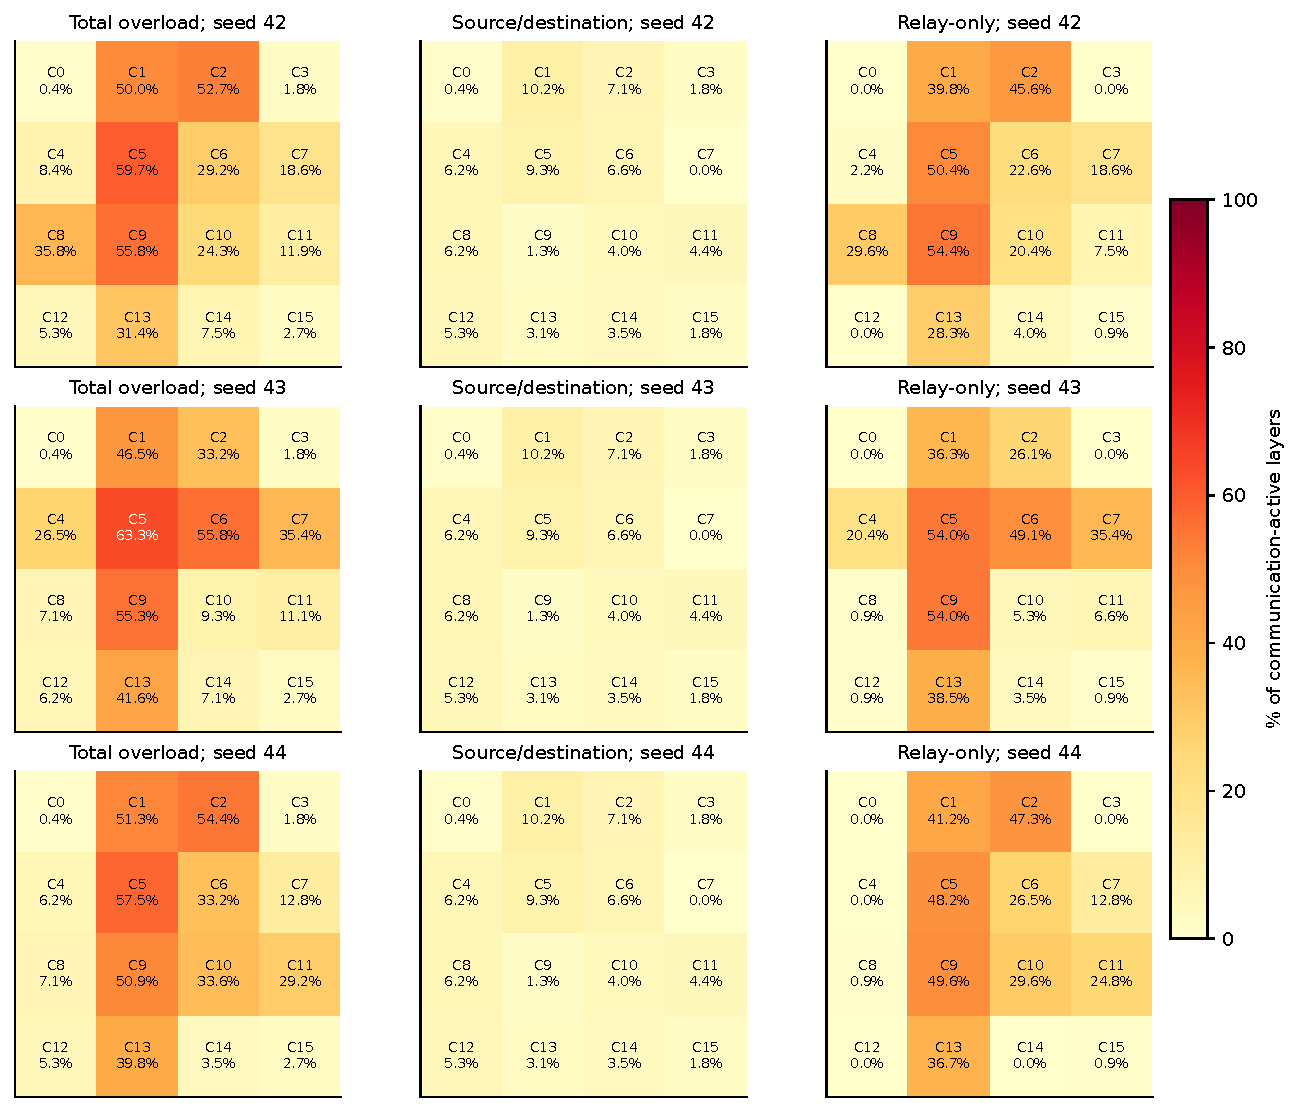
\includegraphics[width=.94\linewidth,height=.48\textheight,keepaspectratio]{figures/atlas/mesh_shortest_reliable_route_m2.pdf}\captionof{figure}{All three conceptual mapping seeds; common 0--100 percent colour scale.}\end{center}
\begin{center}{\scriptsize\setlength{\tabcolsep}{3pt}
\begin{tabular}{lrrrrrrrrr}
\toprule
Core & 42 Tot & 42 Own & 42 Rel & 43 Tot & 43 Own & 43 Rel & 44 Tot & 44 Own & 44 Rel \\
\midrule
0 & 0.442 & 0.442 & 0.000 & 0.442 & 0.442 & 0.000 & 0.442 & 0.442 & 0.000 \\
1 & 50.000 & 10.177 & 39.823 & 46.460 & 10.177 & 36.283 & 51.327 & 10.177 & 41.150 \\
2 & 52.655 & 7.080 & 45.575 & 33.186 & 7.080 & 26.106 & 54.425 & 7.080 & 47.345 \\
3 & 1.770 & 1.770 & 0.000 & 1.770 & 1.770 & 0.000 & 1.770 & 1.770 & 0.000 \\
4 & 8.407 & 6.195 & 2.212 & 26.549 & 6.195 & 20.354 & 6.195 & 6.195 & 0.000 \\
5 & 59.735 & 9.292 & 50.442 & 63.274 & 9.292 & 53.982 & 57.522 & 9.292 & 48.230 \\
6 & 29.204 & 6.637 & 22.566 & 55.752 & 6.637 & 49.115 & 33.186 & 6.637 & 26.549 \\
7 & 18.584 & 0.000 & 18.584 & 35.398 & 0.000 & 35.398 & 12.832 & 0.000 & 12.832 \\
8 & 35.841 & 6.195 & 29.646 & 7.080 & 6.195 & 0.885 & 7.080 & 6.195 & 0.885 \\
9 & 55.752 & 1.327 & 54.425 & 55.310 & 1.327 & 53.982 & 50.885 & 1.327 & 49.558 \\
10 & 24.336 & 3.982 & 20.354 & 9.292 & 3.982 & 5.310 & 33.628 & 3.982 & 29.646 \\
11 & 11.947 & 4.425 & 7.522 & 11.062 & 4.425 & 6.637 & 29.204 & 4.425 & 24.779 \\
12 & 5.310 & 5.310 & 0.000 & 6.195 & 5.310 & 0.885 & 5.310 & 5.310 & 0.000 \\
13 & 31.416 & 3.097 & 28.319 & 41.593 & 3.097 & 38.496 & 39.823 & 3.097 & 36.726 \\
14 & 7.522 & 3.540 & 3.982 & 7.080 & 3.540 & 3.540 & 3.540 & 3.540 & 0.000 \\
15 & 2.655 & 1.770 & 0.885 & 2.655 & 1.770 & 0.885 & 2.655 & 1.770 & 0.885 \\
\bottomrule\end{tabular}}
\captionof{table}{Exact heatmap percentages, with Tot = Own + Rel. Unrounded values are in the CSV.}
{\footnotesize\href{https://github.com/sanjeevkrishnaa/Compiler-Driven-ACE/blob/codex/ace-scheduler-correctness/docs/latex/qft96_final/data/heatmap_mesh_shortest_reliable_route_m2.csv}{Exact CSV values and sample counts}}
\end{center}
\clearpage\subsection*{Mesh shortest\_reliable; M=3; route counting}
\begin{center}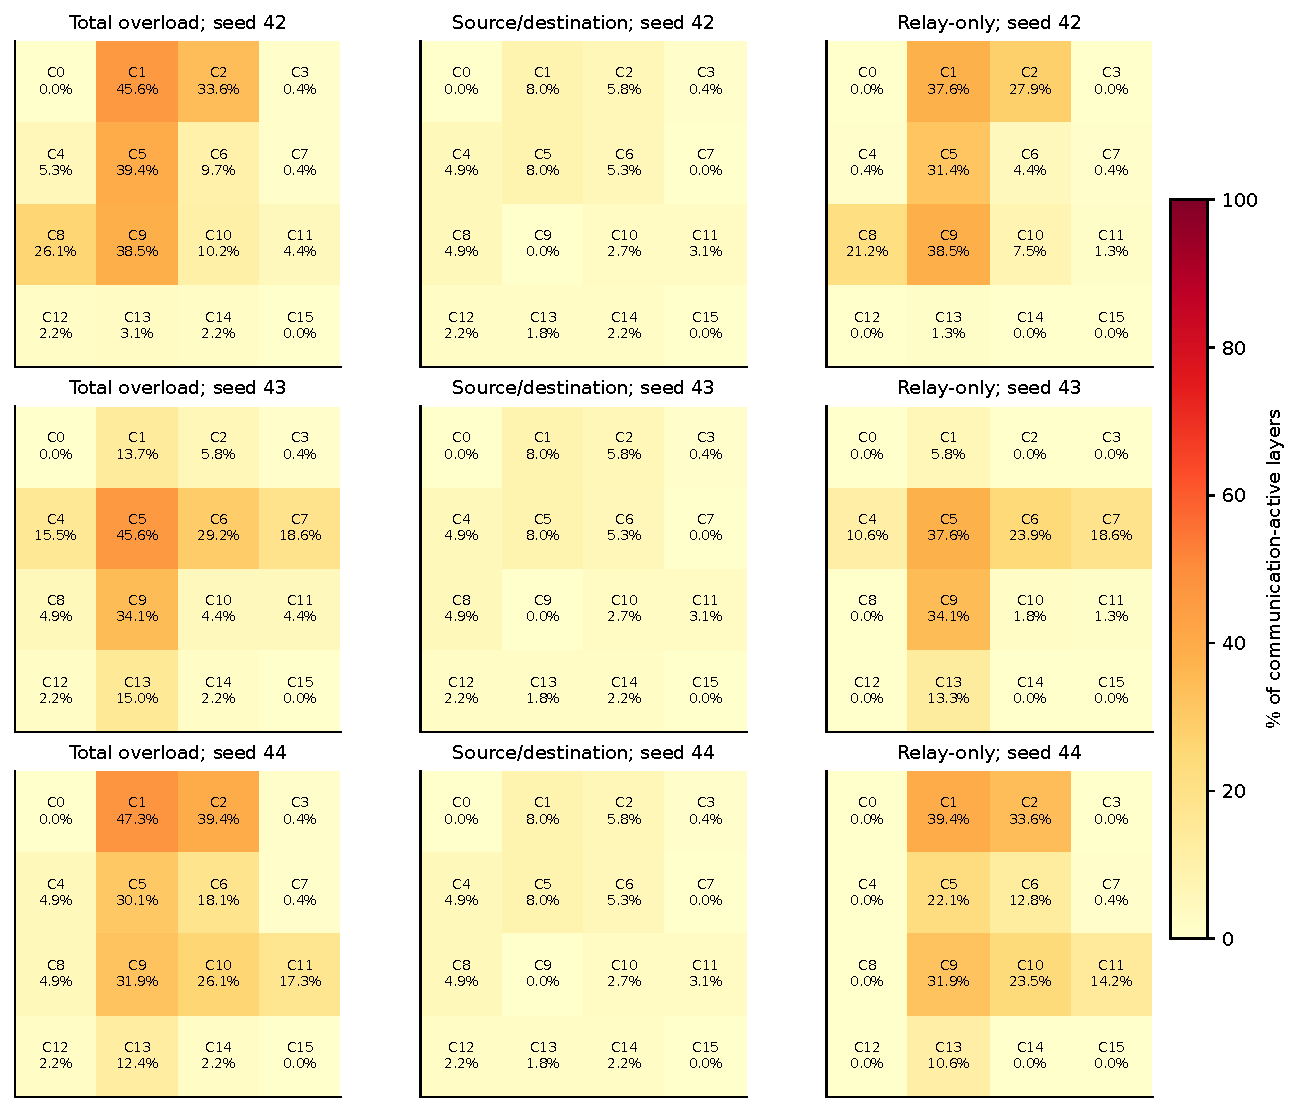
\includegraphics[width=.94\linewidth,height=.48\textheight,keepaspectratio]{figures/atlas/mesh_shortest_reliable_route_m3.pdf}\captionof{figure}{All three conceptual mapping seeds; common 0--100 percent colour scale.}\end{center}
\begin{center}{\scriptsize\setlength{\tabcolsep}{3pt}
\begin{tabular}{lrrrrrrrrr}
\toprule
Core & 42 Tot & 42 Own & 42 Rel & 43 Tot & 43 Own & 43 Rel & 44 Tot & 44 Own & 44 Rel \\
\midrule
0 & 0.000 & 0.000 & 0.000 & 0.000 & 0.000 & 0.000 & 0.000 & 0.000 & 0.000 \\
1 & 45.575 & 7.965 & 37.611 & 13.717 & 7.965 & 5.752 & 47.345 & 7.965 & 39.381 \\
2 & 33.628 & 5.752 & 27.876 & 5.752 & 5.752 & 0.000 & 39.381 & 5.752 & 33.628 \\
3 & 0.442 & 0.442 & 0.000 & 0.442 & 0.442 & 0.000 & 0.442 & 0.442 & 0.000 \\
4 & 5.310 & 4.867 & 0.442 & 15.487 & 4.867 & 10.619 & 4.867 & 4.867 & 0.000 \\
5 & 39.381 & 7.965 & 31.416 & 45.575 & 7.965 & 37.611 & 30.088 & 7.965 & 22.124 \\
6 & 9.735 & 5.310 & 4.425 & 29.204 & 5.310 & 23.894 & 18.142 & 5.310 & 12.832 \\
7 & 0.442 & 0.000 & 0.442 & 18.584 & 0.000 & 18.584 & 0.442 & 0.000 & 0.442 \\
8 & 26.106 & 4.867 & 21.239 & 4.867 & 4.867 & 0.000 & 4.867 & 4.867 & 0.000 \\
9 & 38.496 & 0.000 & 38.496 & 34.071 & 0.000 & 34.071 & 31.858 & 0.000 & 31.858 \\
10 & 10.177 & 2.655 & 7.522 & 4.425 & 2.655 & 1.770 & 26.106 & 2.655 & 23.451 \\
11 & 4.425 & 3.097 & 1.327 & 4.425 & 3.097 & 1.327 & 17.257 & 3.097 & 14.159 \\
12 & 2.212 & 2.212 & 0.000 & 2.212 & 2.212 & 0.000 & 2.212 & 2.212 & 0.000 \\
13 & 3.097 & 1.770 & 1.327 & 15.044 & 1.770 & 13.274 & 12.389 & 1.770 & 10.619 \\
14 & 2.212 & 2.212 & 0.000 & 2.212 & 2.212 & 0.000 & 2.212 & 2.212 & 0.000 \\
15 & 0.000 & 0.000 & 0.000 & 0.000 & 0.000 & 0.000 & 0.000 & 0.000 & 0.000 \\
\bottomrule\end{tabular}}
\captionof{table}{Exact heatmap percentages, with Tot = Own + Rel. Unrounded values are in the CSV.}
{\footnotesize\href{https://github.com/sanjeevkrishnaa/Compiler-Driven-ACE/blob/codex/ace-scheduler-correctness/docs/latex/qft96_final/data/heatmap_mesh_shortest_reliable_route_m3.csv}{Exact CSV values and sample counts}}
\end{center}
\clearpage\subsection*{Mesh shortest\_reliable; M=4; route counting}
\begin{center}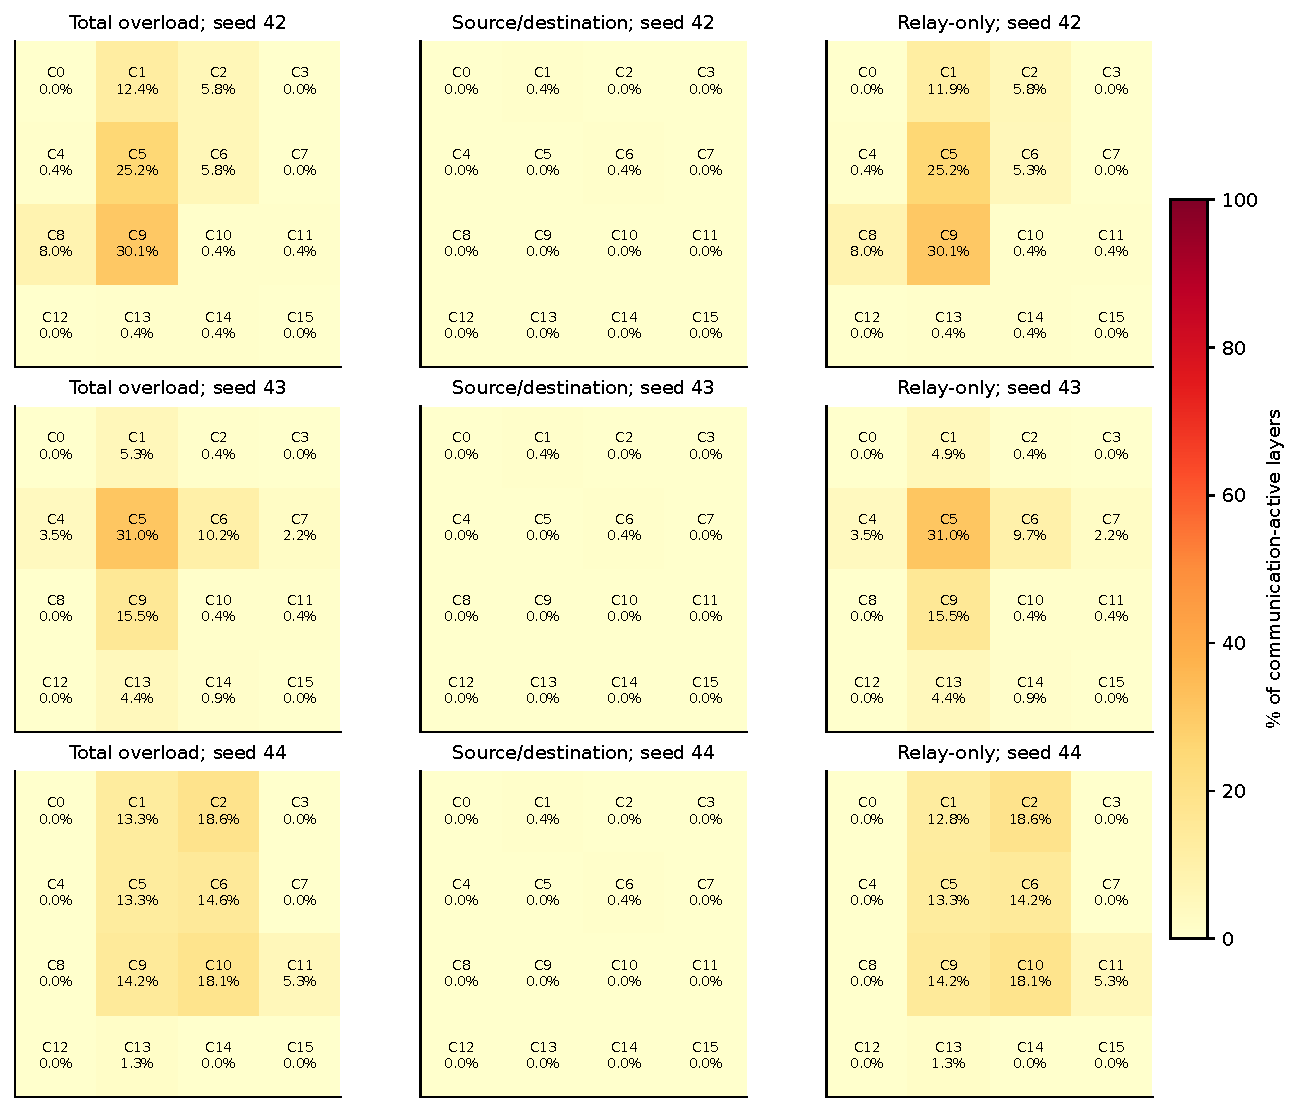
\includegraphics[width=.94\linewidth,height=.48\textheight,keepaspectratio]{figures/atlas/mesh_shortest_reliable_route_m4.pdf}\captionof{figure}{All three conceptual mapping seeds; common 0--100 percent colour scale.}\end{center}
\begin{center}{\scriptsize\setlength{\tabcolsep}{3pt}
\begin{tabular}{lrrrrrrrrr}
\toprule
Core & 42 Tot & 42 Own & 42 Rel & 43 Tot & 43 Own & 43 Rel & 44 Tot & 44 Own & 44 Rel \\
\midrule
0 & 0.000 & 0.000 & 0.000 & 0.000 & 0.000 & 0.000 & 0.000 & 0.000 & 0.000 \\
1 & 12.389 & 0.442 & 11.947 & 5.310 & 0.442 & 4.867 & 13.274 & 0.442 & 12.832 \\
2 & 5.752 & 0.000 & 5.752 & 0.442 & 0.000 & 0.442 & 18.584 & 0.000 & 18.584 \\
3 & 0.000 & 0.000 & 0.000 & 0.000 & 0.000 & 0.000 & 0.000 & 0.000 & 0.000 \\
4 & 0.442 & 0.000 & 0.442 & 3.540 & 0.000 & 3.540 & 0.000 & 0.000 & 0.000 \\
5 & 25.221 & 0.000 & 25.221 & 30.973 & 0.000 & 30.973 & 13.274 & 0.000 & 13.274 \\
6 & 5.752 & 0.442 & 5.310 & 10.177 & 0.442 & 9.735 & 14.602 & 0.442 & 14.159 \\
7 & 0.000 & 0.000 & 0.000 & 2.212 & 0.000 & 2.212 & 0.000 & 0.000 & 0.000 \\
8 & 7.965 & 0.000 & 7.965 & 0.000 & 0.000 & 0.000 & 0.000 & 0.000 & 0.000 \\
9 & 30.088 & 0.000 & 30.088 & 15.487 & 0.000 & 15.487 & 14.159 & 0.000 & 14.159 \\
10 & 0.442 & 0.000 & 0.442 & 0.442 & 0.000 & 0.442 & 18.142 & 0.000 & 18.142 \\
11 & 0.442 & 0.000 & 0.442 & 0.442 & 0.000 & 0.442 & 5.310 & 0.000 & 5.310 \\
12 & 0.000 & 0.000 & 0.000 & 0.000 & 0.000 & 0.000 & 0.000 & 0.000 & 0.000 \\
13 & 0.442 & 0.000 & 0.442 & 4.425 & 0.000 & 4.425 & 1.327 & 0.000 & 1.327 \\
14 & 0.442 & 0.000 & 0.442 & 0.885 & 0.000 & 0.885 & 0.000 & 0.000 & 0.000 \\
15 & 0.000 & 0.000 & 0.000 & 0.000 & 0.000 & 0.000 & 0.000 & 0.000 & 0.000 \\
\bottomrule\end{tabular}}
\captionof{table}{Exact heatmap percentages, with Tot = Own + Rel. Unrounded values are in the CSV.}
{\footnotesize\href{https://github.com/sanjeevkrishnaa/Compiler-Driven-ACE/blob/codex/ace-scheduler-correctness/docs/latex/qft96_final/data/heatmap_mesh_shortest_reliable_route_m4.csv}{Exact CSV values and sample counts}}
\end{center}
\clearpage\subsection*{Mesh shortest\_reliable; M=6; route counting}
\begin{center}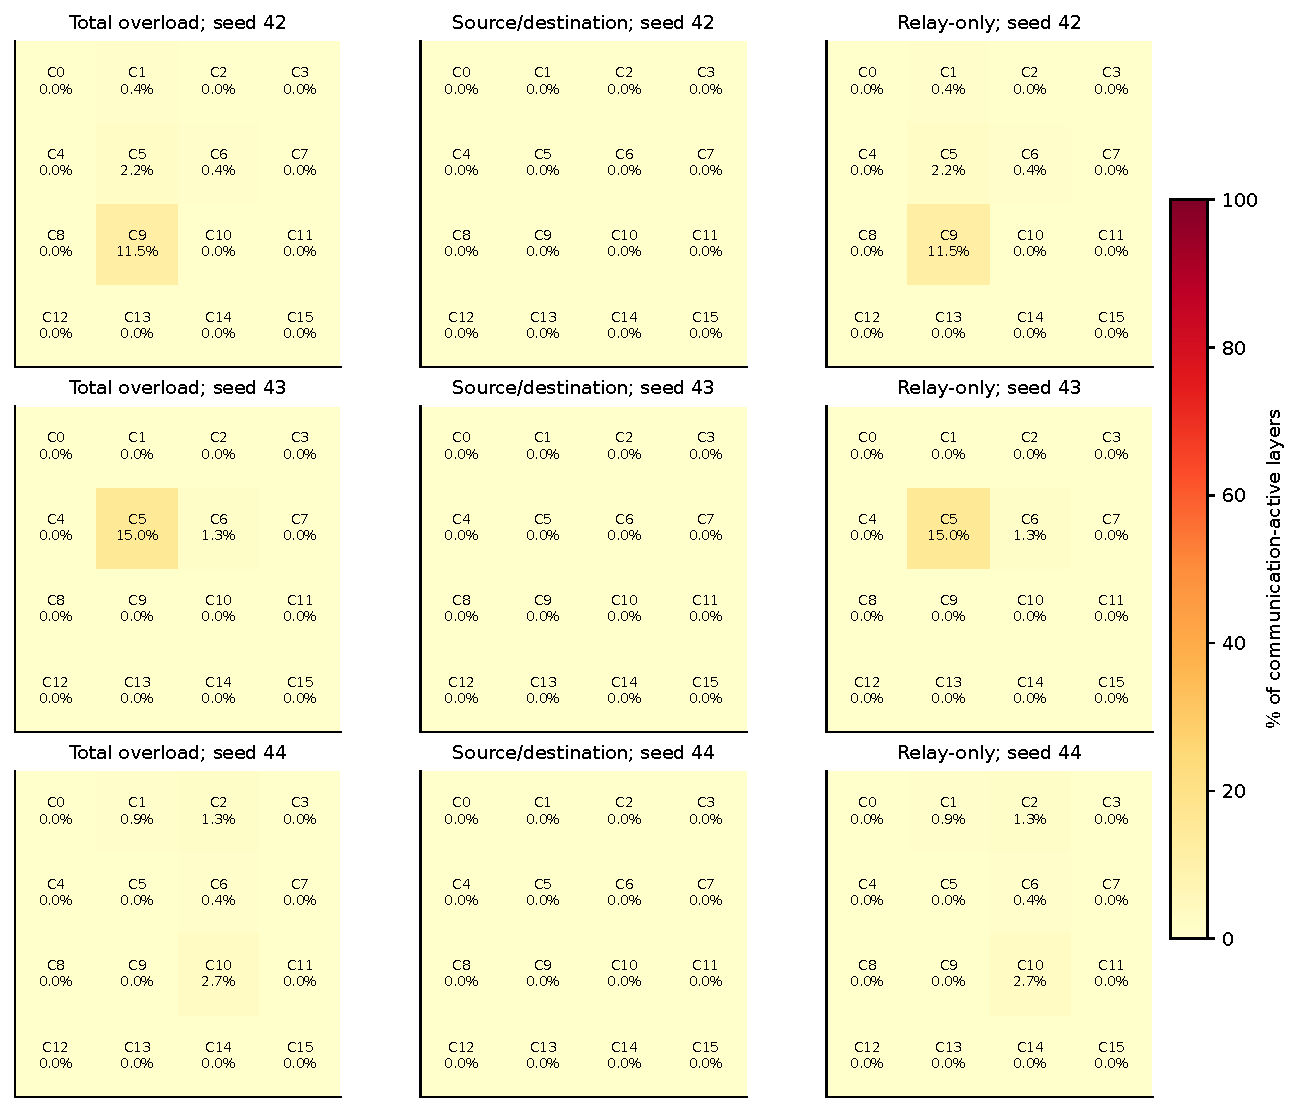
\includegraphics[width=.94\linewidth,height=.48\textheight,keepaspectratio]{figures/atlas/mesh_shortest_reliable_route_m6.pdf}\captionof{figure}{All three conceptual mapping seeds; common 0--100 percent colour scale.}\end{center}
\begin{center}{\scriptsize\setlength{\tabcolsep}{3pt}
\begin{tabular}{lrrrrrrrrr}
\toprule
Core & 42 Tot & 42 Own & 42 Rel & 43 Tot & 43 Own & 43 Rel & 44 Tot & 44 Own & 44 Rel \\
\midrule
0 & 0.000 & 0.000 & 0.000 & 0.000 & 0.000 & 0.000 & 0.000 & 0.000 & 0.000 \\
1 & 0.442 & 0.000 & 0.442 & 0.000 & 0.000 & 0.000 & 0.885 & 0.000 & 0.885 \\
2 & 0.000 & 0.000 & 0.000 & 0.000 & 0.000 & 0.000 & 1.327 & 0.000 & 1.327 \\
3 & 0.000 & 0.000 & 0.000 & 0.000 & 0.000 & 0.000 & 0.000 & 0.000 & 0.000 \\
4 & 0.000 & 0.000 & 0.000 & 0.000 & 0.000 & 0.000 & 0.000 & 0.000 & 0.000 \\
5 & 2.212 & 0.000 & 2.212 & 15.044 & 0.000 & 15.044 & 0.000 & 0.000 & 0.000 \\
6 & 0.442 & 0.000 & 0.442 & 1.327 & 0.000 & 1.327 & 0.442 & 0.000 & 0.442 \\
7 & 0.000 & 0.000 & 0.000 & 0.000 & 0.000 & 0.000 & 0.000 & 0.000 & 0.000 \\
8 & 0.000 & 0.000 & 0.000 & 0.000 & 0.000 & 0.000 & 0.000 & 0.000 & 0.000 \\
9 & 11.504 & 0.000 & 11.504 & 0.000 & 0.000 & 0.000 & 0.000 & 0.000 & 0.000 \\
10 & 0.000 & 0.000 & 0.000 & 0.000 & 0.000 & 0.000 & 2.655 & 0.000 & 2.655 \\
11 & 0.000 & 0.000 & 0.000 & 0.000 & 0.000 & 0.000 & 0.000 & 0.000 & 0.000 \\
12 & 0.000 & 0.000 & 0.000 & 0.000 & 0.000 & 0.000 & 0.000 & 0.000 & 0.000 \\
13 & 0.000 & 0.000 & 0.000 & 0.000 & 0.000 & 0.000 & 0.000 & 0.000 & 0.000 \\
14 & 0.000 & 0.000 & 0.000 & 0.000 & 0.000 & 0.000 & 0.000 & 0.000 & 0.000 \\
15 & 0.000 & 0.000 & 0.000 & 0.000 & 0.000 & 0.000 & 0.000 & 0.000 & 0.000 \\
\bottomrule\end{tabular}}
\captionof{table}{Exact heatmap percentages, with Tot = Own + Rel. Unrounded values are in the CSV.}
{\footnotesize\href{https://github.com/sanjeevkrishnaa/Compiler-Driven-ACE/blob/codex/ace-scheduler-correctness/docs/latex/qft96_final/data/heatmap_mesh_shortest_reliable_route_m6.csv}{Exact CSV values and sample counts}}
\end{center}
\clearpage\subsection*{Mesh shortest\_reliable; M=8; route counting}
\begin{center}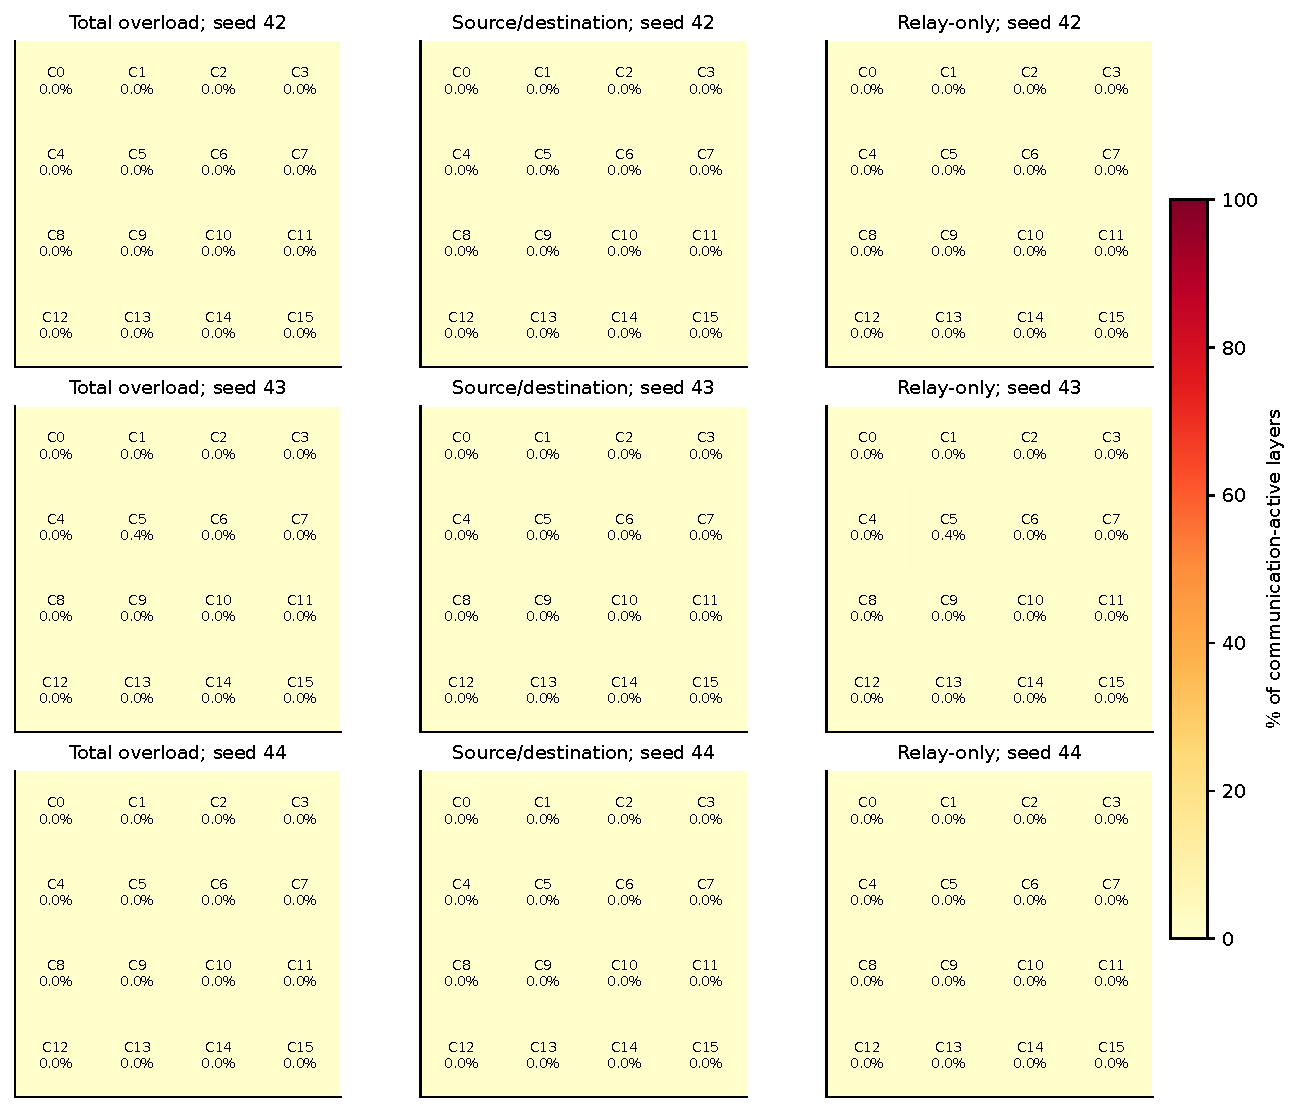
\includegraphics[width=.94\linewidth,height=.48\textheight,keepaspectratio]{figures/atlas/mesh_shortest_reliable_route_m8.pdf}\captionof{figure}{All three conceptual mapping seeds; common 0--100 percent colour scale.}\end{center}
\begin{center}{\scriptsize\setlength{\tabcolsep}{3pt}
\begin{tabular}{lrrrrrrrrr}
\toprule
Core & 42 Tot & 42 Own & 42 Rel & 43 Tot & 43 Own & 43 Rel & 44 Tot & 44 Own & 44 Rel \\
\midrule
0 & 0.000 & 0.000 & 0.000 & 0.000 & 0.000 & 0.000 & 0.000 & 0.000 & 0.000 \\
1 & 0.000 & 0.000 & 0.000 & 0.000 & 0.000 & 0.000 & 0.000 & 0.000 & 0.000 \\
2 & 0.000 & 0.000 & 0.000 & 0.000 & 0.000 & 0.000 & 0.000 & 0.000 & 0.000 \\
3 & 0.000 & 0.000 & 0.000 & 0.000 & 0.000 & 0.000 & 0.000 & 0.000 & 0.000 \\
4 & 0.000 & 0.000 & 0.000 & 0.000 & 0.000 & 0.000 & 0.000 & 0.000 & 0.000 \\
5 & 0.000 & 0.000 & 0.000 & 0.442 & 0.000 & 0.442 & 0.000 & 0.000 & 0.000 \\
6 & 0.000 & 0.000 & 0.000 & 0.000 & 0.000 & 0.000 & 0.000 & 0.000 & 0.000 \\
7 & 0.000 & 0.000 & 0.000 & 0.000 & 0.000 & 0.000 & 0.000 & 0.000 & 0.000 \\
8 & 0.000 & 0.000 & 0.000 & 0.000 & 0.000 & 0.000 & 0.000 & 0.000 & 0.000 \\
9 & 0.000 & 0.000 & 0.000 & 0.000 & 0.000 & 0.000 & 0.000 & 0.000 & 0.000 \\
10 & 0.000 & 0.000 & 0.000 & 0.000 & 0.000 & 0.000 & 0.000 & 0.000 & 0.000 \\
11 & 0.000 & 0.000 & 0.000 & 0.000 & 0.000 & 0.000 & 0.000 & 0.000 & 0.000 \\
12 & 0.000 & 0.000 & 0.000 & 0.000 & 0.000 & 0.000 & 0.000 & 0.000 & 0.000 \\
13 & 0.000 & 0.000 & 0.000 & 0.000 & 0.000 & 0.000 & 0.000 & 0.000 & 0.000 \\
14 & 0.000 & 0.000 & 0.000 & 0.000 & 0.000 & 0.000 & 0.000 & 0.000 & 0.000 \\
15 & 0.000 & 0.000 & 0.000 & 0.000 & 0.000 & 0.000 & 0.000 & 0.000 & 0.000 \\
\bottomrule\end{tabular}}
\captionof{table}{Exact heatmap percentages, with Tot = Own + Rel. Unrounded values are in the CSV.}
{\footnotesize\href{https://github.com/sanjeevkrishnaa/Compiler-Driven-ACE/blob/codex/ace-scheduler-correctness/docs/latex/qft96_final/data/heatmap_mesh_shortest_reliable_route_m8.csv}{Exact CSV values and sample counts}}
\end{center}
\clearpage\subsection*{Mesh shortest\_reliable; M=16; route counting}
\begin{center}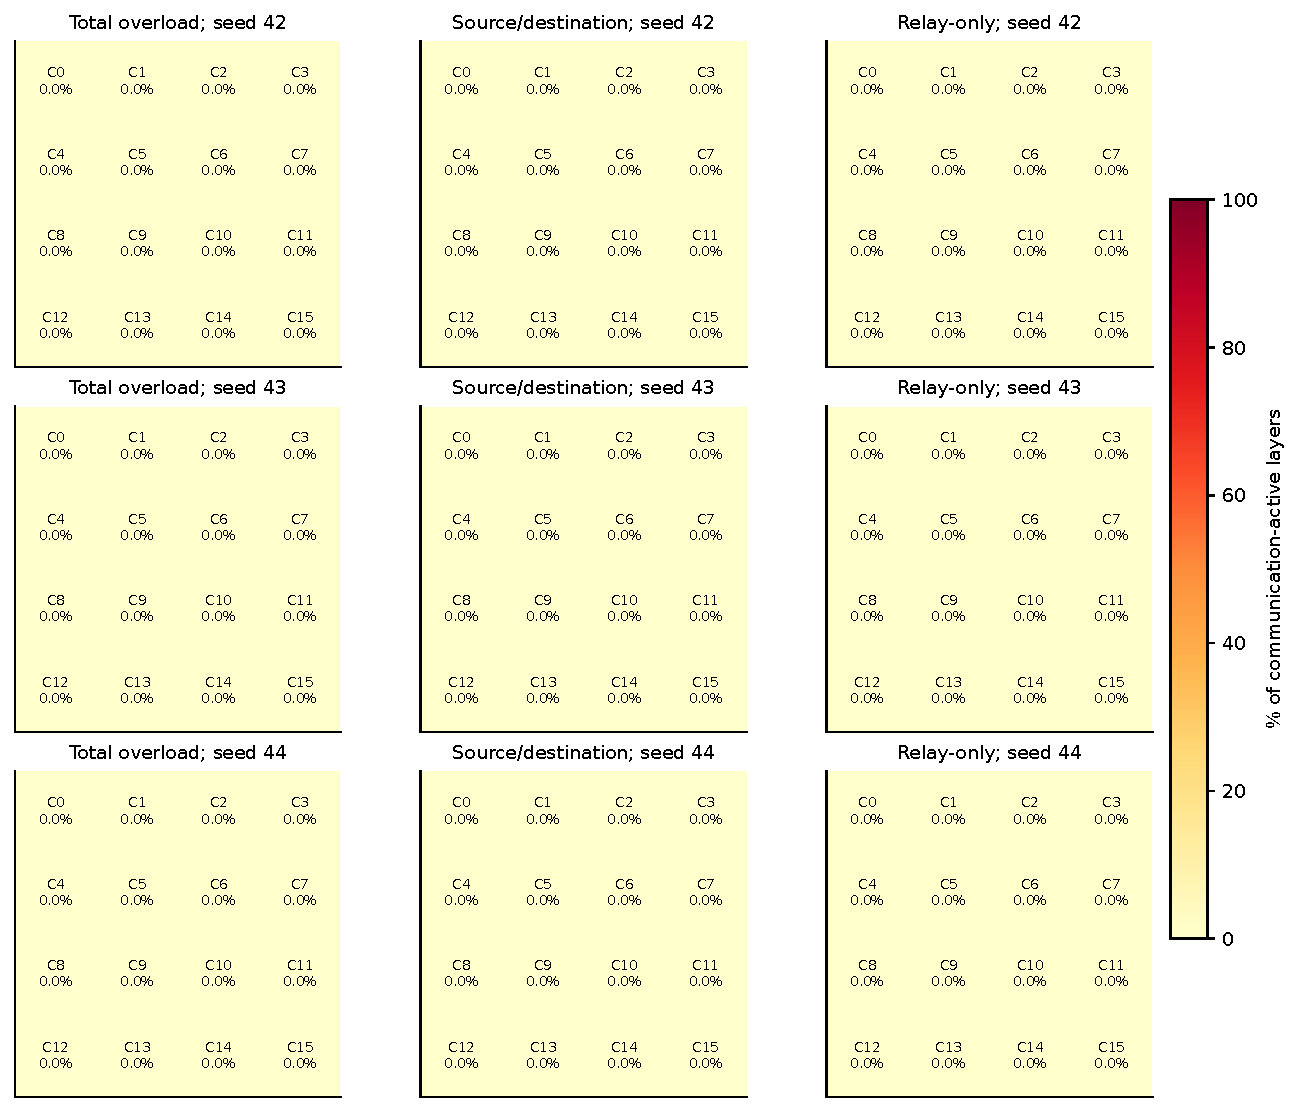
\includegraphics[width=.94\linewidth,height=.48\textheight,keepaspectratio]{figures/atlas/mesh_shortest_reliable_route_m16.pdf}\captionof{figure}{All three conceptual mapping seeds; common 0--100 percent colour scale.}\end{center}
\begin{center}{\scriptsize\setlength{\tabcolsep}{3pt}
\begin{tabular}{lrrrrrrrrr}
\toprule
Core & 42 Tot & 42 Own & 42 Rel & 43 Tot & 43 Own & 43 Rel & 44 Tot & 44 Own & 44 Rel \\
\midrule
0 & 0.000 & 0.000 & 0.000 & 0.000 & 0.000 & 0.000 & 0.000 & 0.000 & 0.000 \\
1 & 0.000 & 0.000 & 0.000 & 0.000 & 0.000 & 0.000 & 0.000 & 0.000 & 0.000 \\
2 & 0.000 & 0.000 & 0.000 & 0.000 & 0.000 & 0.000 & 0.000 & 0.000 & 0.000 \\
3 & 0.000 & 0.000 & 0.000 & 0.000 & 0.000 & 0.000 & 0.000 & 0.000 & 0.000 \\
4 & 0.000 & 0.000 & 0.000 & 0.000 & 0.000 & 0.000 & 0.000 & 0.000 & 0.000 \\
5 & 0.000 & 0.000 & 0.000 & 0.000 & 0.000 & 0.000 & 0.000 & 0.000 & 0.000 \\
6 & 0.000 & 0.000 & 0.000 & 0.000 & 0.000 & 0.000 & 0.000 & 0.000 & 0.000 \\
7 & 0.000 & 0.000 & 0.000 & 0.000 & 0.000 & 0.000 & 0.000 & 0.000 & 0.000 \\
8 & 0.000 & 0.000 & 0.000 & 0.000 & 0.000 & 0.000 & 0.000 & 0.000 & 0.000 \\
9 & 0.000 & 0.000 & 0.000 & 0.000 & 0.000 & 0.000 & 0.000 & 0.000 & 0.000 \\
10 & 0.000 & 0.000 & 0.000 & 0.000 & 0.000 & 0.000 & 0.000 & 0.000 & 0.000 \\
11 & 0.000 & 0.000 & 0.000 & 0.000 & 0.000 & 0.000 & 0.000 & 0.000 & 0.000 \\
12 & 0.000 & 0.000 & 0.000 & 0.000 & 0.000 & 0.000 & 0.000 & 0.000 & 0.000 \\
13 & 0.000 & 0.000 & 0.000 & 0.000 & 0.000 & 0.000 & 0.000 & 0.000 & 0.000 \\
14 & 0.000 & 0.000 & 0.000 & 0.000 & 0.000 & 0.000 & 0.000 & 0.000 & 0.000 \\
15 & 0.000 & 0.000 & 0.000 & 0.000 & 0.000 & 0.000 & 0.000 & 0.000 & 0.000 \\
\bottomrule\end{tabular}}
\captionof{table}{Exact heatmap percentages, with Tot = Own + Rel. Unrounded values are in the CSV.}
{\footnotesize\href{https://github.com/sanjeevkrishnaa/Compiler-Driven-ACE/blob/codex/ace-scheduler-correctness/docs/latex/qft96_final/data/heatmap_mesh_shortest_reliable_route_m16.csv}{Exact CSV values and sample counts}}
\end{center}
\clearpage\subsection*{Mesh shortest\_reliable; M=32; route counting}
\begin{center}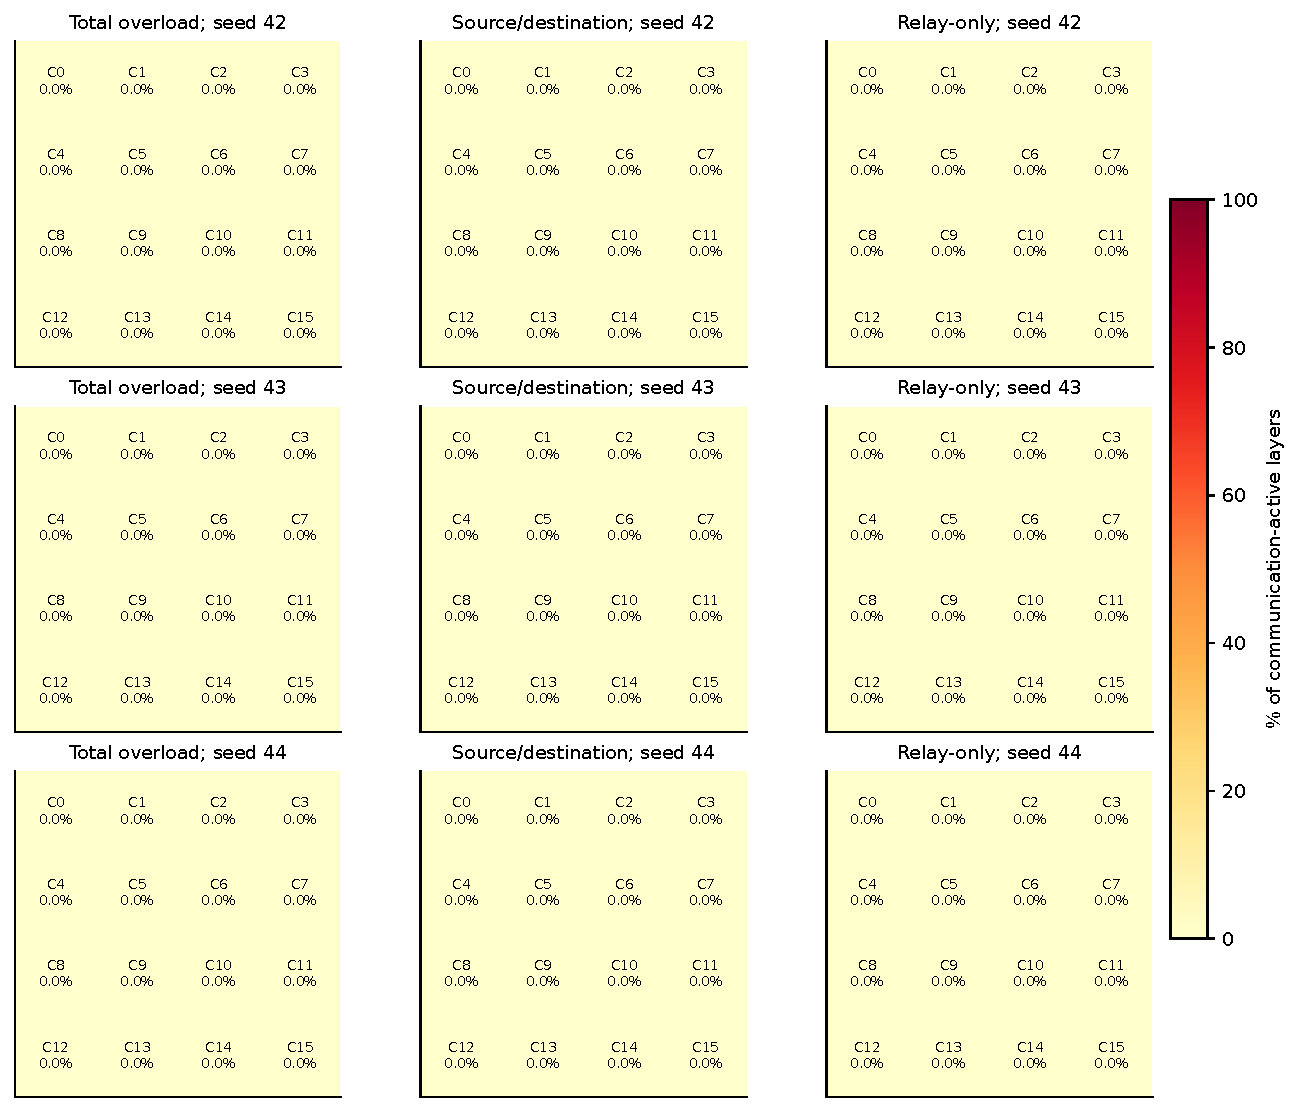
\includegraphics[width=.94\linewidth,height=.48\textheight,keepaspectratio]{figures/atlas/mesh_shortest_reliable_route_m32.pdf}\captionof{figure}{All three conceptual mapping seeds; common 0--100 percent colour scale.}\end{center}
\begin{center}{\scriptsize\setlength{\tabcolsep}{3pt}
\begin{tabular}{lrrrrrrrrr}
\toprule
Core & 42 Tot & 42 Own & 42 Rel & 43 Tot & 43 Own & 43 Rel & 44 Tot & 44 Own & 44 Rel \\
\midrule
0 & 0.000 & 0.000 & 0.000 & 0.000 & 0.000 & 0.000 & 0.000 & 0.000 & 0.000 \\
1 & 0.000 & 0.000 & 0.000 & 0.000 & 0.000 & 0.000 & 0.000 & 0.000 & 0.000 \\
2 & 0.000 & 0.000 & 0.000 & 0.000 & 0.000 & 0.000 & 0.000 & 0.000 & 0.000 \\
3 & 0.000 & 0.000 & 0.000 & 0.000 & 0.000 & 0.000 & 0.000 & 0.000 & 0.000 \\
4 & 0.000 & 0.000 & 0.000 & 0.000 & 0.000 & 0.000 & 0.000 & 0.000 & 0.000 \\
5 & 0.000 & 0.000 & 0.000 & 0.000 & 0.000 & 0.000 & 0.000 & 0.000 & 0.000 \\
6 & 0.000 & 0.000 & 0.000 & 0.000 & 0.000 & 0.000 & 0.000 & 0.000 & 0.000 \\
7 & 0.000 & 0.000 & 0.000 & 0.000 & 0.000 & 0.000 & 0.000 & 0.000 & 0.000 \\
8 & 0.000 & 0.000 & 0.000 & 0.000 & 0.000 & 0.000 & 0.000 & 0.000 & 0.000 \\
9 & 0.000 & 0.000 & 0.000 & 0.000 & 0.000 & 0.000 & 0.000 & 0.000 & 0.000 \\
10 & 0.000 & 0.000 & 0.000 & 0.000 & 0.000 & 0.000 & 0.000 & 0.000 & 0.000 \\
11 & 0.000 & 0.000 & 0.000 & 0.000 & 0.000 & 0.000 & 0.000 & 0.000 & 0.000 \\
12 & 0.000 & 0.000 & 0.000 & 0.000 & 0.000 & 0.000 & 0.000 & 0.000 & 0.000 \\
13 & 0.000 & 0.000 & 0.000 & 0.000 & 0.000 & 0.000 & 0.000 & 0.000 & 0.000 \\
14 & 0.000 & 0.000 & 0.000 & 0.000 & 0.000 & 0.000 & 0.000 & 0.000 & 0.000 \\
15 & 0.000 & 0.000 & 0.000 & 0.000 & 0.000 & 0.000 & 0.000 & 0.000 & 0.000 \\
\bottomrule\end{tabular}}
\captionof{table}{Exact heatmap percentages, with Tot = Own + Rel. Unrounded values are in the CSV.}
{\footnotesize\href{https://github.com/sanjeevkrishnaa/Compiler-Driven-ACE/blob/codex/ace-scheduler-correctness/docs/latex/qft96_final/data/heatmap_mesh_shortest_reliable_route_m32.csv}{Exact CSV values and sample counts}}
\end{center}
\clearpage\subsection*{Mesh shortest\_reliable; M=2; hop counting}
\begin{center}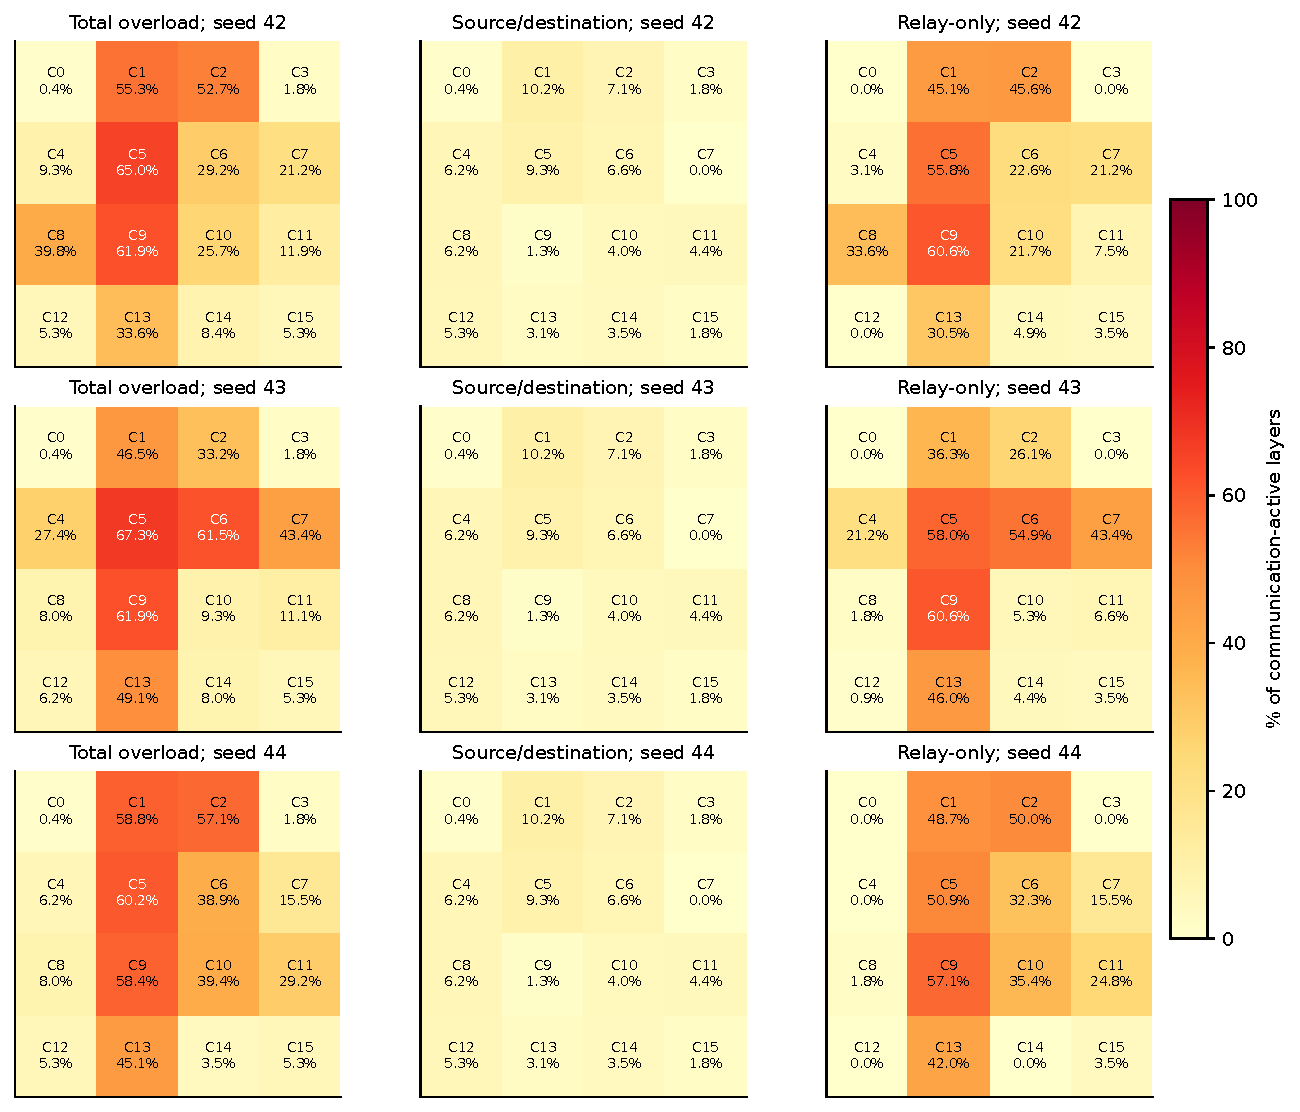
\includegraphics[width=.94\linewidth,height=.48\textheight,keepaspectratio]{figures/atlas/mesh_shortest_reliable_hop_m2.pdf}\captionof{figure}{All three conceptual mapping seeds; common 0--100 percent colour scale.}\end{center}
\begin{center}{\scriptsize\setlength{\tabcolsep}{3pt}
\begin{tabular}{lrrrrrrrrr}
\toprule
Core & 42 Tot & 42 Own & 42 Rel & 43 Tot & 43 Own & 43 Rel & 44 Tot & 44 Own & 44 Rel \\
\midrule
0 & 0.442 & 0.442 & 0.000 & 0.442 & 0.442 & 0.000 & 0.442 & 0.442 & 0.000 \\
1 & 55.310 & 10.177 & 45.133 & 46.460 & 10.177 & 36.283 & 58.850 & 10.177 & 48.673 \\
2 & 52.655 & 7.080 & 45.575 & 33.186 & 7.080 & 26.106 & 57.080 & 7.080 & 50.000 \\
3 & 1.770 & 1.770 & 0.000 & 1.770 & 1.770 & 0.000 & 1.770 & 1.770 & 0.000 \\
4 & 9.292 & 6.195 & 3.097 & 27.434 & 6.195 & 21.239 & 6.195 & 6.195 & 0.000 \\
5 & 65.044 & 9.292 & 55.752 & 67.257 & 9.292 & 57.965 & 60.177 & 9.292 & 50.885 \\
6 & 29.204 & 6.637 & 22.566 & 61.504 & 6.637 & 54.867 & 38.938 & 6.637 & 32.301 \\
7 & 21.239 & 0.000 & 21.239 & 43.363 & 0.000 & 43.363 & 15.487 & 0.000 & 15.487 \\
8 & 39.823 & 6.195 & 33.628 & 7.965 & 6.195 & 1.770 & 7.965 & 6.195 & 1.770 \\
9 & 61.947 & 1.327 & 60.619 & 61.947 & 1.327 & 60.619 & 58.407 & 1.327 & 57.080 \\
10 & 25.664 & 3.982 & 21.681 & 9.292 & 3.982 & 5.310 & 39.381 & 3.982 & 35.398 \\
11 & 11.947 & 4.425 & 7.522 & 11.062 & 4.425 & 6.637 & 29.204 & 4.425 & 24.779 \\
12 & 5.310 & 5.310 & 0.000 & 6.195 & 5.310 & 0.885 & 5.310 & 5.310 & 0.000 \\
13 & 33.628 & 3.097 & 30.531 & 49.115 & 3.097 & 46.018 & 45.133 & 3.097 & 42.035 \\
14 & 8.407 & 3.540 & 4.867 & 7.965 & 3.540 & 4.425 & 3.540 & 3.540 & 0.000 \\
15 & 5.310 & 1.770 & 3.540 & 5.310 & 1.770 & 3.540 & 5.310 & 1.770 & 3.540 \\
\bottomrule\end{tabular}}
\captionof{table}{Exact heatmap percentages, with Tot = Own + Rel. Unrounded values are in the CSV.}
{\footnotesize\href{https://github.com/sanjeevkrishnaa/Compiler-Driven-ACE/blob/codex/ace-scheduler-correctness/docs/latex/qft96_final/data/heatmap_mesh_shortest_reliable_hop_m2.csv}{Exact CSV values and sample counts}}
\end{center}
\clearpage\subsection*{Mesh shortest\_reliable; M=3; hop counting}
\begin{center}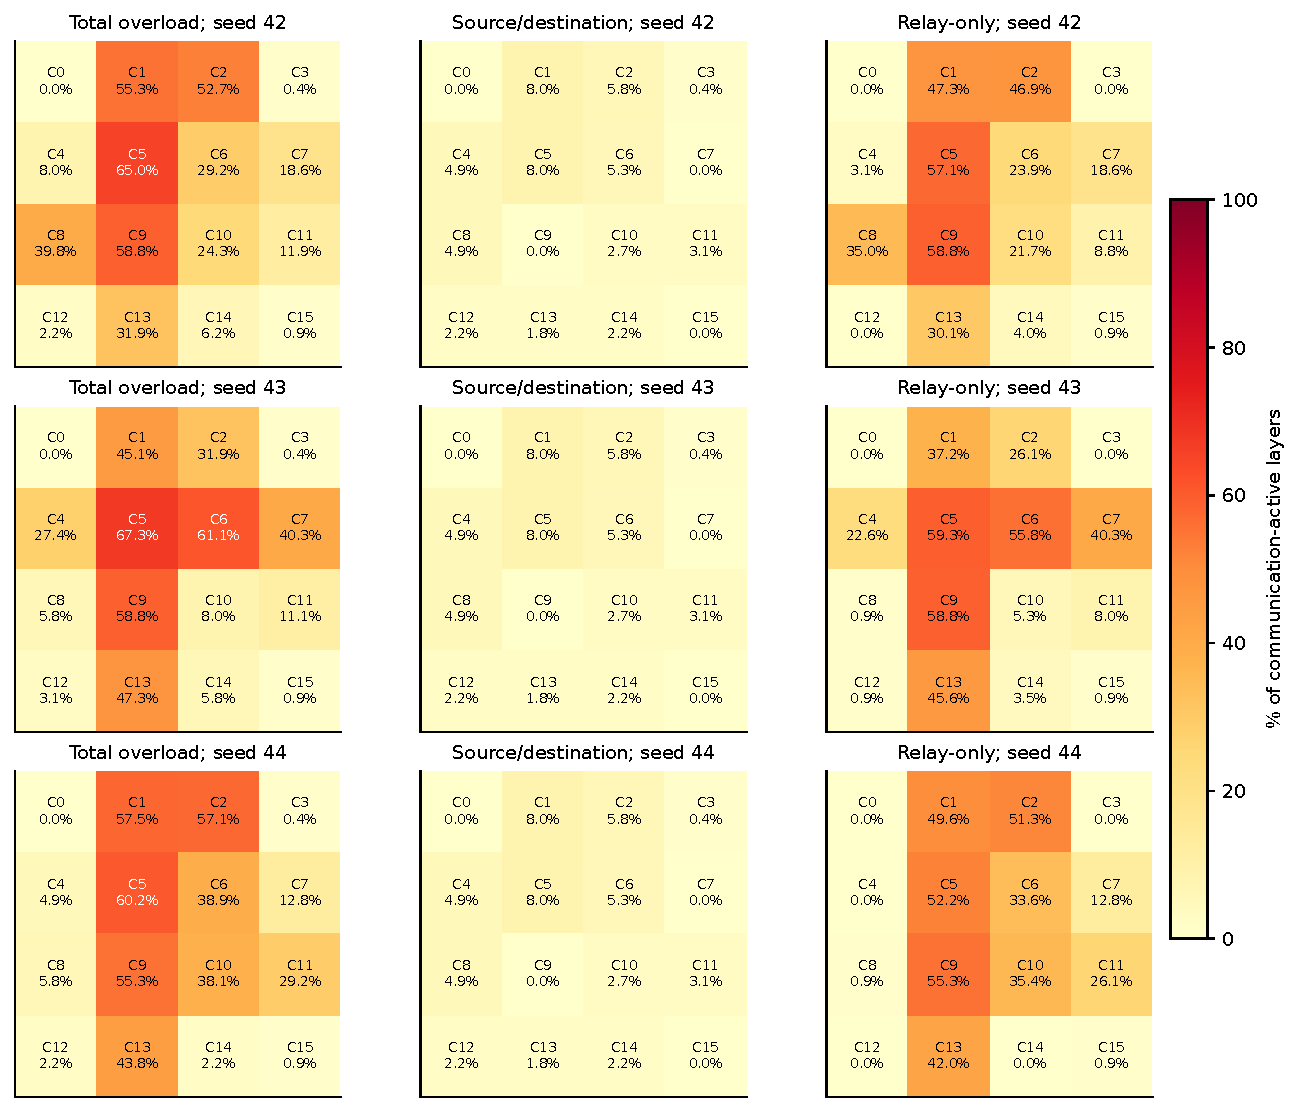
\includegraphics[width=.94\linewidth,height=.48\textheight,keepaspectratio]{figures/atlas/mesh_shortest_reliable_hop_m3.pdf}\captionof{figure}{All three conceptual mapping seeds; common 0--100 percent colour scale.}\end{center}
\begin{center}{\scriptsize\setlength{\tabcolsep}{3pt}
\begin{tabular}{lrrrrrrrrr}
\toprule
Core & 42 Tot & 42 Own & 42 Rel & 43 Tot & 43 Own & 43 Rel & 44 Tot & 44 Own & 44 Rel \\
\midrule
0 & 0.000 & 0.000 & 0.000 & 0.000 & 0.000 & 0.000 & 0.000 & 0.000 & 0.000 \\
1 & 55.310 & 7.965 & 47.345 & 45.133 & 7.965 & 37.168 & 57.522 & 7.965 & 49.558 \\
2 & 52.655 & 5.752 & 46.903 & 31.858 & 5.752 & 26.106 & 57.080 & 5.752 & 51.327 \\
3 & 0.442 & 0.442 & 0.000 & 0.442 & 0.442 & 0.000 & 0.442 & 0.442 & 0.000 \\
4 & 7.965 & 4.867 & 3.097 & 27.434 & 4.867 & 22.566 & 4.867 & 4.867 & 0.000 \\
5 & 65.044 & 7.965 & 57.080 & 67.257 & 7.965 & 59.292 & 60.177 & 7.965 & 52.212 \\
6 & 29.204 & 5.310 & 23.894 & 61.062 & 5.310 & 55.752 & 38.938 & 5.310 & 33.628 \\
7 & 18.584 & 0.000 & 18.584 & 40.265 & 0.000 & 40.265 & 12.832 & 0.000 & 12.832 \\
8 & 39.823 & 4.867 & 34.956 & 5.752 & 4.867 & 0.885 & 5.752 & 4.867 & 0.885 \\
9 & 58.850 & 0.000 & 58.850 & 58.850 & 0.000 & 58.850 & 55.310 & 0.000 & 55.310 \\
10 & 24.336 & 2.655 & 21.681 & 7.965 & 2.655 & 5.310 & 38.053 & 2.655 & 35.398 \\
11 & 11.947 & 3.097 & 8.850 & 11.062 & 3.097 & 7.965 & 29.204 & 3.097 & 26.106 \\
12 & 2.212 & 2.212 & 0.000 & 3.097 & 2.212 & 0.885 & 2.212 & 2.212 & 0.000 \\
13 & 31.858 & 1.770 & 30.088 & 47.345 & 1.770 & 45.575 & 43.805 & 1.770 & 42.035 \\
14 & 6.195 & 2.212 & 3.982 & 5.752 & 2.212 & 3.540 & 2.212 & 2.212 & 0.000 \\
15 & 0.885 & 0.000 & 0.885 & 0.885 & 0.000 & 0.885 & 0.885 & 0.000 & 0.885 \\
\bottomrule\end{tabular}}
\captionof{table}{Exact heatmap percentages, with Tot = Own + Rel. Unrounded values are in the CSV.}
{\footnotesize\href{https://github.com/sanjeevkrishnaa/Compiler-Driven-ACE/blob/codex/ace-scheduler-correctness/docs/latex/qft96_final/data/heatmap_mesh_shortest_reliable_hop_m3.csv}{Exact CSV values and sample counts}}
\end{center}
\clearpage\subsection*{Mesh shortest\_reliable; M=4; hop counting}
\begin{center}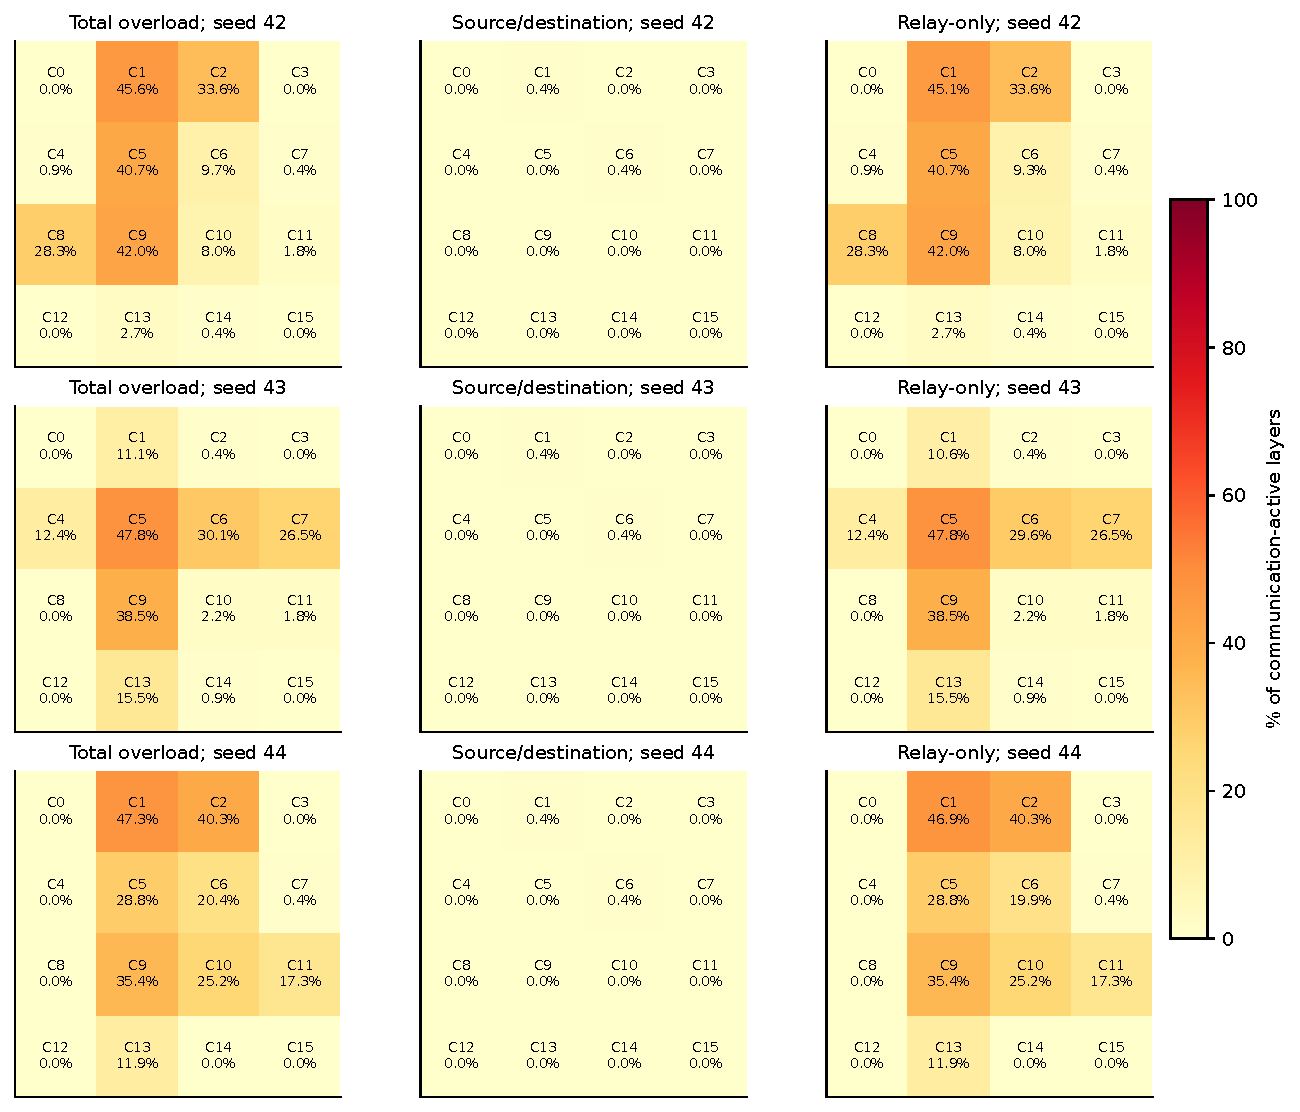
\includegraphics[width=.94\linewidth,height=.48\textheight,keepaspectratio]{figures/atlas/mesh_shortest_reliable_hop_m4.pdf}\captionof{figure}{All three conceptual mapping seeds; common 0--100 percent colour scale.}\end{center}
\begin{center}{\scriptsize\setlength{\tabcolsep}{3pt}
\begin{tabular}{lrrrrrrrrr}
\toprule
Core & 42 Tot & 42 Own & 42 Rel & 43 Tot & 43 Own & 43 Rel & 44 Tot & 44 Own & 44 Rel \\
\midrule
0 & 0.000 & 0.000 & 0.000 & 0.000 & 0.000 & 0.000 & 0.000 & 0.000 & 0.000 \\
1 & 45.575 & 0.442 & 45.133 & 11.062 & 0.442 & 10.619 & 47.345 & 0.442 & 46.903 \\
2 & 33.628 & 0.000 & 33.628 & 0.442 & 0.000 & 0.442 & 40.265 & 0.000 & 40.265 \\
3 & 0.000 & 0.000 & 0.000 & 0.000 & 0.000 & 0.000 & 0.000 & 0.000 & 0.000 \\
4 & 0.885 & 0.000 & 0.885 & 12.389 & 0.000 & 12.389 & 0.000 & 0.000 & 0.000 \\
5 & 40.708 & 0.000 & 40.708 & 47.788 & 0.000 & 47.788 & 28.761 & 0.000 & 28.761 \\
6 & 9.735 & 0.442 & 9.292 & 30.088 & 0.442 & 29.646 & 20.354 & 0.442 & 19.912 \\
7 & 0.442 & 0.000 & 0.442 & 26.549 & 0.000 & 26.549 & 0.442 & 0.000 & 0.442 \\
8 & 28.319 & 0.000 & 28.319 & 0.000 & 0.000 & 0.000 & 0.000 & 0.000 & 0.000 \\
9 & 42.035 & 0.000 & 42.035 & 38.496 & 0.000 & 38.496 & 35.398 & 0.000 & 35.398 \\
10 & 7.965 & 0.000 & 7.965 & 2.212 & 0.000 & 2.212 & 25.221 & 0.000 & 25.221 \\
11 & 1.770 & 0.000 & 1.770 & 1.770 & 0.000 & 1.770 & 17.257 & 0.000 & 17.257 \\
12 & 0.000 & 0.000 & 0.000 & 0.000 & 0.000 & 0.000 & 0.000 & 0.000 & 0.000 \\
13 & 2.655 & 0.000 & 2.655 & 15.487 & 0.000 & 15.487 & 11.947 & 0.000 & 11.947 \\
14 & 0.442 & 0.000 & 0.442 & 0.885 & 0.000 & 0.885 & 0.000 & 0.000 & 0.000 \\
15 & 0.000 & 0.000 & 0.000 & 0.000 & 0.000 & 0.000 & 0.000 & 0.000 & 0.000 \\
\bottomrule\end{tabular}}
\captionof{table}{Exact heatmap percentages, with Tot = Own + Rel. Unrounded values are in the CSV.}
{\footnotesize\href{https://github.com/sanjeevkrishnaa/Compiler-Driven-ACE/blob/codex/ace-scheduler-correctness/docs/latex/qft96_final/data/heatmap_mesh_shortest_reliable_hop_m4.csv}{Exact CSV values and sample counts}}
\end{center}
\clearpage\subsection*{Mesh shortest\_reliable; M=6; hop counting}
\begin{center}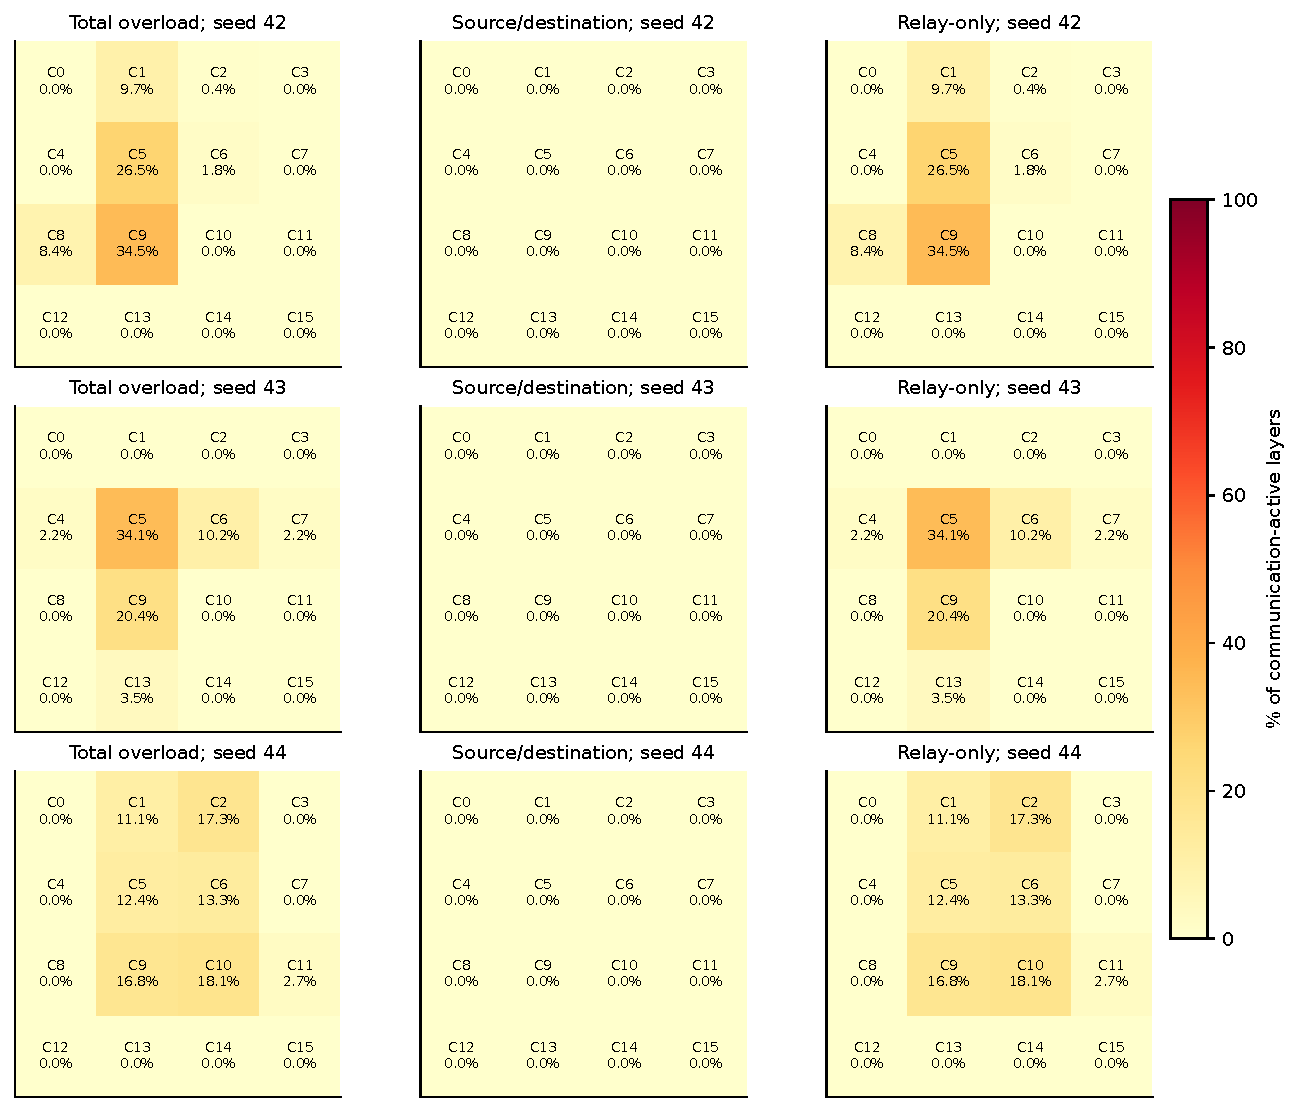
\includegraphics[width=.94\linewidth,height=.48\textheight,keepaspectratio]{figures/atlas/mesh_shortest_reliable_hop_m6.pdf}\captionof{figure}{All three conceptual mapping seeds; common 0--100 percent colour scale.}\end{center}
\begin{center}{\scriptsize\setlength{\tabcolsep}{3pt}
\begin{tabular}{lrrrrrrrrr}
\toprule
Core & 42 Tot & 42 Own & 42 Rel & 43 Tot & 43 Own & 43 Rel & 44 Tot & 44 Own & 44 Rel \\
\midrule
0 & 0.000 & 0.000 & 0.000 & 0.000 & 0.000 & 0.000 & 0.000 & 0.000 & 0.000 \\
1 & 9.735 & 0.000 & 9.735 & 0.000 & 0.000 & 0.000 & 11.062 & 0.000 & 11.062 \\
2 & 0.442 & 0.000 & 0.442 & 0.000 & 0.000 & 0.000 & 17.257 & 0.000 & 17.257 \\
3 & 0.000 & 0.000 & 0.000 & 0.000 & 0.000 & 0.000 & 0.000 & 0.000 & 0.000 \\
4 & 0.000 & 0.000 & 0.000 & 2.212 & 0.000 & 2.212 & 0.000 & 0.000 & 0.000 \\
5 & 26.549 & 0.000 & 26.549 & 34.071 & 0.000 & 34.071 & 12.389 & 0.000 & 12.389 \\
6 & 1.770 & 0.000 & 1.770 & 10.177 & 0.000 & 10.177 & 13.274 & 0.000 & 13.274 \\
7 & 0.000 & 0.000 & 0.000 & 2.212 & 0.000 & 2.212 & 0.000 & 0.000 & 0.000 \\
8 & 8.407 & 0.000 & 8.407 & 0.000 & 0.000 & 0.000 & 0.000 & 0.000 & 0.000 \\
9 & 34.513 & 0.000 & 34.513 & 20.354 & 0.000 & 20.354 & 16.814 & 0.000 & 16.814 \\
10 & 0.000 & 0.000 & 0.000 & 0.000 & 0.000 & 0.000 & 18.142 & 0.000 & 18.142 \\
11 & 0.000 & 0.000 & 0.000 & 0.000 & 0.000 & 0.000 & 2.655 & 0.000 & 2.655 \\
12 & 0.000 & 0.000 & 0.000 & 0.000 & 0.000 & 0.000 & 0.000 & 0.000 & 0.000 \\
13 & 0.000 & 0.000 & 0.000 & 3.540 & 0.000 & 3.540 & 0.000 & 0.000 & 0.000 \\
14 & 0.000 & 0.000 & 0.000 & 0.000 & 0.000 & 0.000 & 0.000 & 0.000 & 0.000 \\
15 & 0.000 & 0.000 & 0.000 & 0.000 & 0.000 & 0.000 & 0.000 & 0.000 & 0.000 \\
\bottomrule\end{tabular}}
\captionof{table}{Exact heatmap percentages, with Tot = Own + Rel. Unrounded values are in the CSV.}
{\footnotesize\href{https://github.com/sanjeevkrishnaa/Compiler-Driven-ACE/blob/codex/ace-scheduler-correctness/docs/latex/qft96_final/data/heatmap_mesh_shortest_reliable_hop_m6.csv}{Exact CSV values and sample counts}}
\end{center}
\clearpage\subsection*{Mesh shortest\_reliable; M=8; hop counting}
\begin{center}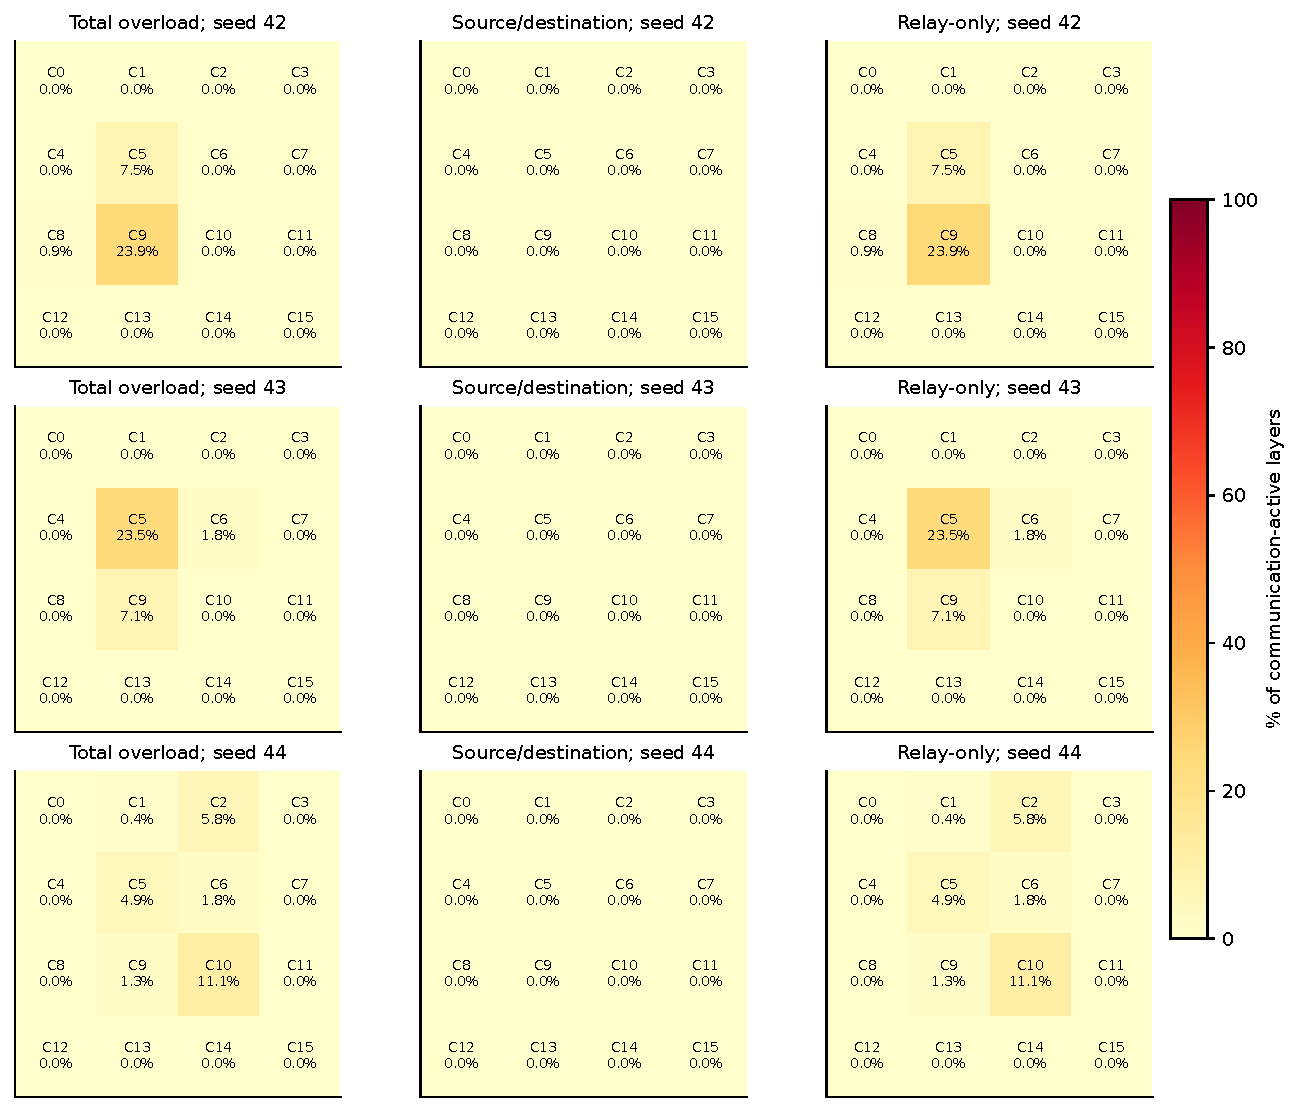
\includegraphics[width=.94\linewidth,height=.48\textheight,keepaspectratio]{figures/atlas/mesh_shortest_reliable_hop_m8.pdf}\captionof{figure}{All three conceptual mapping seeds; common 0--100 percent colour scale.}\end{center}
\begin{center}{\scriptsize\setlength{\tabcolsep}{3pt}
\begin{tabular}{lrrrrrrrrr}
\toprule
Core & 42 Tot & 42 Own & 42 Rel & 43 Tot & 43 Own & 43 Rel & 44 Tot & 44 Own & 44 Rel \\
\midrule
0 & 0.000 & 0.000 & 0.000 & 0.000 & 0.000 & 0.000 & 0.000 & 0.000 & 0.000 \\
1 & 0.000 & 0.000 & 0.000 & 0.000 & 0.000 & 0.000 & 0.442 & 0.000 & 0.442 \\
2 & 0.000 & 0.000 & 0.000 & 0.000 & 0.000 & 0.000 & 5.752 & 0.000 & 5.752 \\
3 & 0.000 & 0.000 & 0.000 & 0.000 & 0.000 & 0.000 & 0.000 & 0.000 & 0.000 \\
4 & 0.000 & 0.000 & 0.000 & 0.000 & 0.000 & 0.000 & 0.000 & 0.000 & 0.000 \\
5 & 7.522 & 0.000 & 7.522 & 23.451 & 0.000 & 23.451 & 4.867 & 0.000 & 4.867 \\
6 & 0.000 & 0.000 & 0.000 & 1.770 & 0.000 & 1.770 & 1.770 & 0.000 & 1.770 \\
7 & 0.000 & 0.000 & 0.000 & 0.000 & 0.000 & 0.000 & 0.000 & 0.000 & 0.000 \\
8 & 0.885 & 0.000 & 0.885 & 0.000 & 0.000 & 0.000 & 0.000 & 0.000 & 0.000 \\
9 & 23.894 & 0.000 & 23.894 & 7.080 & 0.000 & 7.080 & 1.327 & 0.000 & 1.327 \\
10 & 0.000 & 0.000 & 0.000 & 0.000 & 0.000 & 0.000 & 11.062 & 0.000 & 11.062 \\
11 & 0.000 & 0.000 & 0.000 & 0.000 & 0.000 & 0.000 & 0.000 & 0.000 & 0.000 \\
12 & 0.000 & 0.000 & 0.000 & 0.000 & 0.000 & 0.000 & 0.000 & 0.000 & 0.000 \\
13 & 0.000 & 0.000 & 0.000 & 0.000 & 0.000 & 0.000 & 0.000 & 0.000 & 0.000 \\
14 & 0.000 & 0.000 & 0.000 & 0.000 & 0.000 & 0.000 & 0.000 & 0.000 & 0.000 \\
15 & 0.000 & 0.000 & 0.000 & 0.000 & 0.000 & 0.000 & 0.000 & 0.000 & 0.000 \\
\bottomrule\end{tabular}}
\captionof{table}{Exact heatmap percentages, with Tot = Own + Rel. Unrounded values are in the CSV.}
{\footnotesize\href{https://github.com/sanjeevkrishnaa/Compiler-Driven-ACE/blob/codex/ace-scheduler-correctness/docs/latex/qft96_final/data/heatmap_mesh_shortest_reliable_hop_m8.csv}{Exact CSV values and sample counts}}
\end{center}
\clearpage\subsection*{Mesh shortest\_reliable; M=16; hop counting}
\begin{center}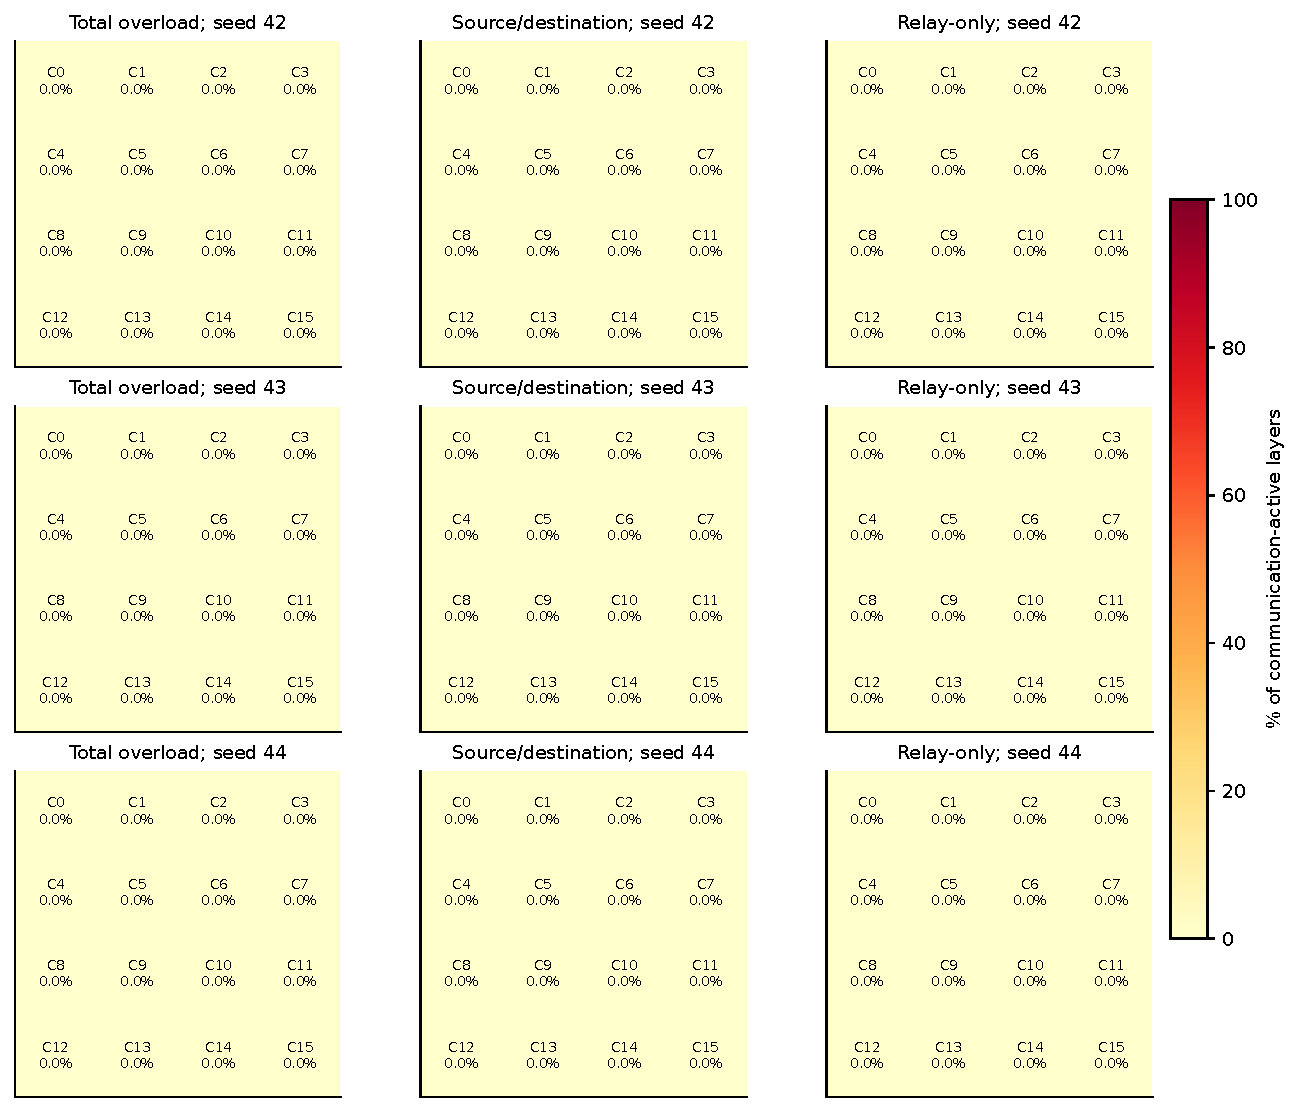
\includegraphics[width=.94\linewidth,height=.48\textheight,keepaspectratio]{figures/atlas/mesh_shortest_reliable_hop_m16.pdf}\captionof{figure}{All three conceptual mapping seeds; common 0--100 percent colour scale.}\end{center}
\begin{center}{\scriptsize\setlength{\tabcolsep}{3pt}
\begin{tabular}{lrrrrrrrrr}
\toprule
Core & 42 Tot & 42 Own & 42 Rel & 43 Tot & 43 Own & 43 Rel & 44 Tot & 44 Own & 44 Rel \\
\midrule
0 & 0.000 & 0.000 & 0.000 & 0.000 & 0.000 & 0.000 & 0.000 & 0.000 & 0.000 \\
1 & 0.000 & 0.000 & 0.000 & 0.000 & 0.000 & 0.000 & 0.000 & 0.000 & 0.000 \\
2 & 0.000 & 0.000 & 0.000 & 0.000 & 0.000 & 0.000 & 0.000 & 0.000 & 0.000 \\
3 & 0.000 & 0.000 & 0.000 & 0.000 & 0.000 & 0.000 & 0.000 & 0.000 & 0.000 \\
4 & 0.000 & 0.000 & 0.000 & 0.000 & 0.000 & 0.000 & 0.000 & 0.000 & 0.000 \\
5 & 0.000 & 0.000 & 0.000 & 0.000 & 0.000 & 0.000 & 0.000 & 0.000 & 0.000 \\
6 & 0.000 & 0.000 & 0.000 & 0.000 & 0.000 & 0.000 & 0.000 & 0.000 & 0.000 \\
7 & 0.000 & 0.000 & 0.000 & 0.000 & 0.000 & 0.000 & 0.000 & 0.000 & 0.000 \\
8 & 0.000 & 0.000 & 0.000 & 0.000 & 0.000 & 0.000 & 0.000 & 0.000 & 0.000 \\
9 & 0.000 & 0.000 & 0.000 & 0.000 & 0.000 & 0.000 & 0.000 & 0.000 & 0.000 \\
10 & 0.000 & 0.000 & 0.000 & 0.000 & 0.000 & 0.000 & 0.000 & 0.000 & 0.000 \\
11 & 0.000 & 0.000 & 0.000 & 0.000 & 0.000 & 0.000 & 0.000 & 0.000 & 0.000 \\
12 & 0.000 & 0.000 & 0.000 & 0.000 & 0.000 & 0.000 & 0.000 & 0.000 & 0.000 \\
13 & 0.000 & 0.000 & 0.000 & 0.000 & 0.000 & 0.000 & 0.000 & 0.000 & 0.000 \\
14 & 0.000 & 0.000 & 0.000 & 0.000 & 0.000 & 0.000 & 0.000 & 0.000 & 0.000 \\
15 & 0.000 & 0.000 & 0.000 & 0.000 & 0.000 & 0.000 & 0.000 & 0.000 & 0.000 \\
\bottomrule\end{tabular}}
\captionof{table}{Exact heatmap percentages, with Tot = Own + Rel. Unrounded values are in the CSV.}
{\footnotesize\href{https://github.com/sanjeevkrishnaa/Compiler-Driven-ACE/blob/codex/ace-scheduler-correctness/docs/latex/qft96_final/data/heatmap_mesh_shortest_reliable_hop_m16.csv}{Exact CSV values and sample counts}}
\end{center}
\clearpage\subsection*{Mesh shortest\_reliable; M=32; hop counting}
\begin{center}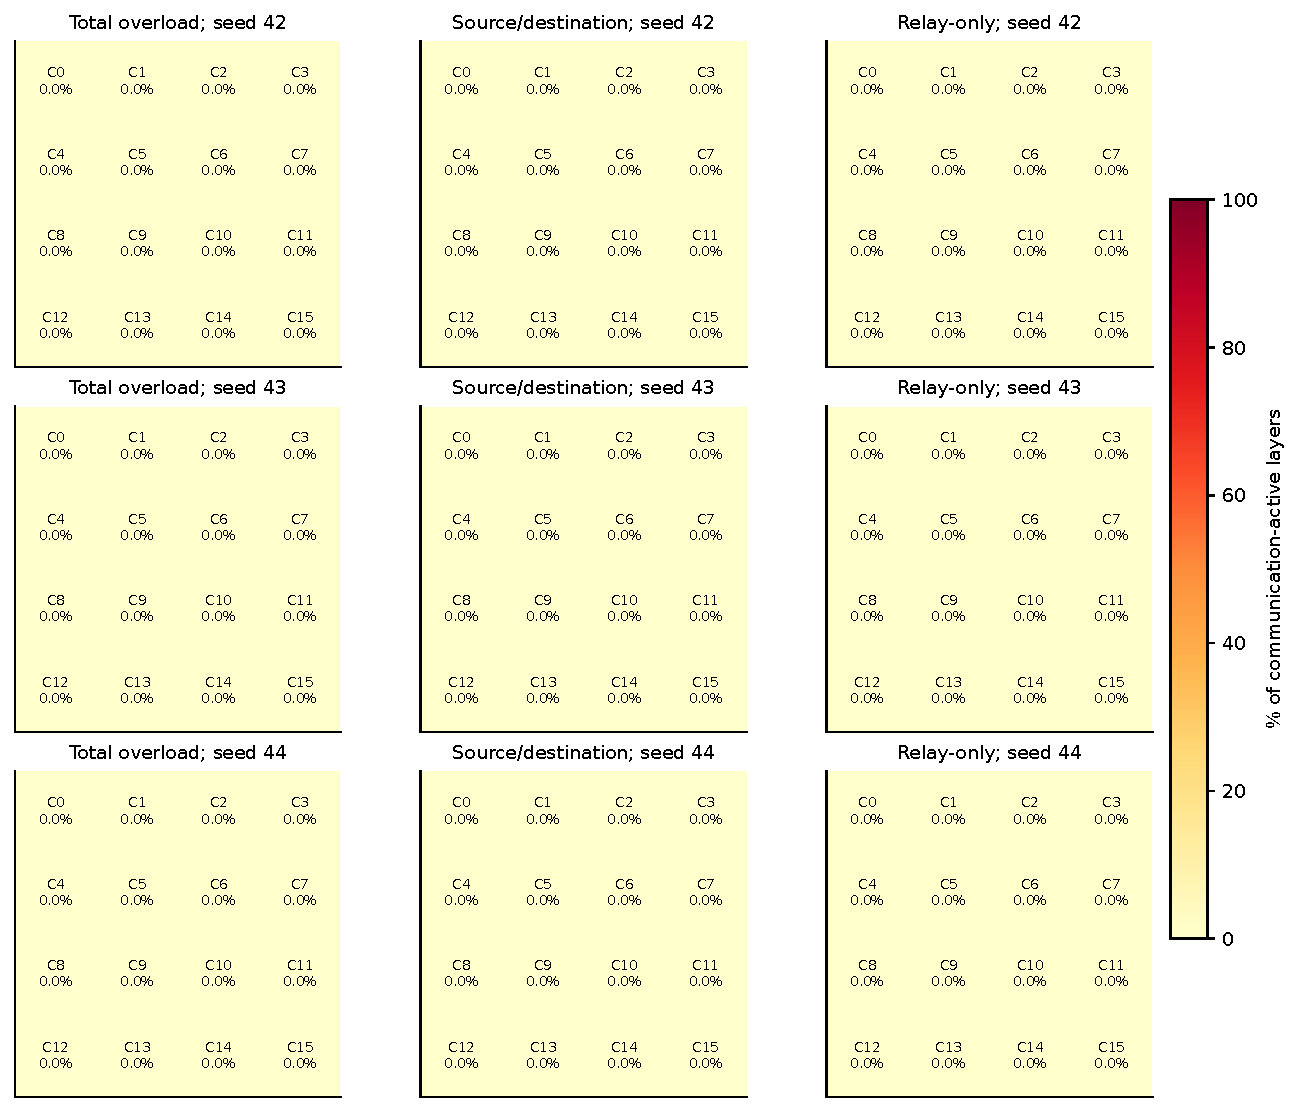
\includegraphics[width=.94\linewidth,height=.48\textheight,keepaspectratio]{figures/atlas/mesh_shortest_reliable_hop_m32.pdf}\captionof{figure}{All three conceptual mapping seeds; common 0--100 percent colour scale.}\end{center}
\begin{center}{\scriptsize\setlength{\tabcolsep}{3pt}
\begin{tabular}{lrrrrrrrrr}
\toprule
Core & 42 Tot & 42 Own & 42 Rel & 43 Tot & 43 Own & 43 Rel & 44 Tot & 44 Own & 44 Rel \\
\midrule
0 & 0.000 & 0.000 & 0.000 & 0.000 & 0.000 & 0.000 & 0.000 & 0.000 & 0.000 \\
1 & 0.000 & 0.000 & 0.000 & 0.000 & 0.000 & 0.000 & 0.000 & 0.000 & 0.000 \\
2 & 0.000 & 0.000 & 0.000 & 0.000 & 0.000 & 0.000 & 0.000 & 0.000 & 0.000 \\
3 & 0.000 & 0.000 & 0.000 & 0.000 & 0.000 & 0.000 & 0.000 & 0.000 & 0.000 \\
4 & 0.000 & 0.000 & 0.000 & 0.000 & 0.000 & 0.000 & 0.000 & 0.000 & 0.000 \\
5 & 0.000 & 0.000 & 0.000 & 0.000 & 0.000 & 0.000 & 0.000 & 0.000 & 0.000 \\
6 & 0.000 & 0.000 & 0.000 & 0.000 & 0.000 & 0.000 & 0.000 & 0.000 & 0.000 \\
7 & 0.000 & 0.000 & 0.000 & 0.000 & 0.000 & 0.000 & 0.000 & 0.000 & 0.000 \\
8 & 0.000 & 0.000 & 0.000 & 0.000 & 0.000 & 0.000 & 0.000 & 0.000 & 0.000 \\
9 & 0.000 & 0.000 & 0.000 & 0.000 & 0.000 & 0.000 & 0.000 & 0.000 & 0.000 \\
10 & 0.000 & 0.000 & 0.000 & 0.000 & 0.000 & 0.000 & 0.000 & 0.000 & 0.000 \\
11 & 0.000 & 0.000 & 0.000 & 0.000 & 0.000 & 0.000 & 0.000 & 0.000 & 0.000 \\
12 & 0.000 & 0.000 & 0.000 & 0.000 & 0.000 & 0.000 & 0.000 & 0.000 & 0.000 \\
13 & 0.000 & 0.000 & 0.000 & 0.000 & 0.000 & 0.000 & 0.000 & 0.000 & 0.000 \\
14 & 0.000 & 0.000 & 0.000 & 0.000 & 0.000 & 0.000 & 0.000 & 0.000 & 0.000 \\
15 & 0.000 & 0.000 & 0.000 & 0.000 & 0.000 & 0.000 & 0.000 & 0.000 & 0.000 \\
\bottomrule\end{tabular}}
\captionof{table}{Exact heatmap percentages, with Tot = Own + Rel. Unrounded values are in the CSV.}
{\footnotesize\href{https://github.com/sanjeevkrishnaa/Compiler-Driven-ACE/blob/codex/ace-scheduler-correctness/docs/latex/qft96_final/data/heatmap_mesh_shortest_reliable_hop_m32.csv}{Exact CSV values and sample counts}}
\end{center}
\section{Mesh / max\_reliability}
\clearpage\subsection*{Mesh max\_reliability; M=2; route counting}
\begin{center}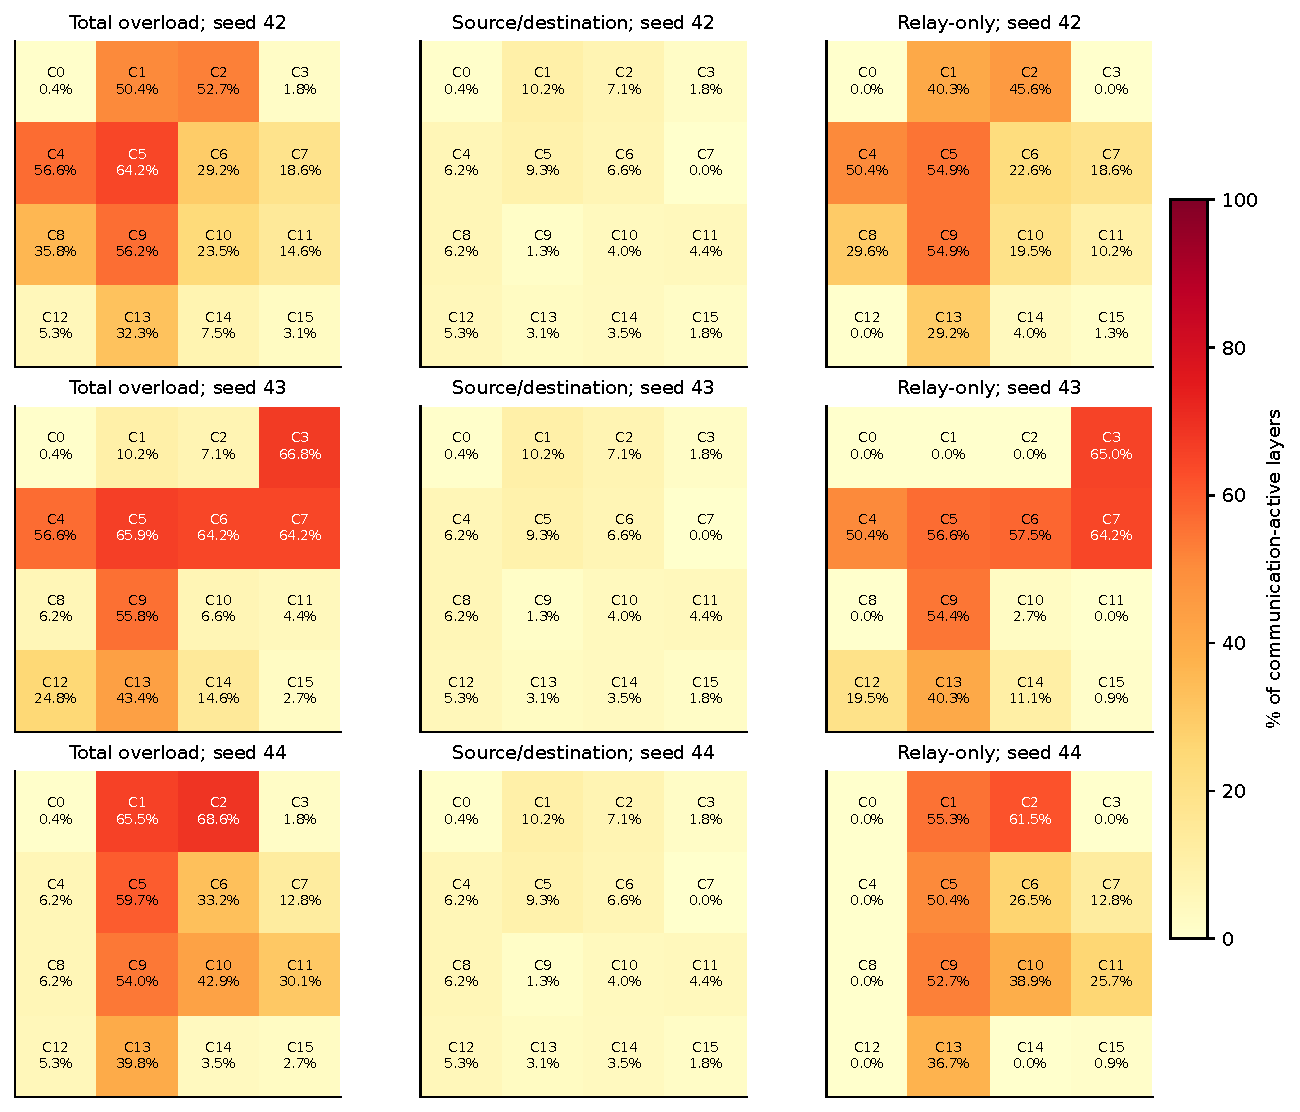
\includegraphics[width=.94\linewidth,height=.48\textheight,keepaspectratio]{figures/atlas/mesh_max_reliability_route_m2.pdf}\captionof{figure}{All three conceptual mapping seeds; common 0--100 percent colour scale.}\end{center}
\begin{center}{\scriptsize\setlength{\tabcolsep}{3pt}
\begin{tabular}{lrrrrrrrrr}
\toprule
Core & 42 Tot & 42 Own & 42 Rel & 43 Tot & 43 Own & 43 Rel & 44 Tot & 44 Own & 44 Rel \\
\midrule
0 & 0.442 & 0.442 & 0.000 & 0.442 & 0.442 & 0.000 & 0.442 & 0.442 & 0.000 \\
1 & 50.442 & 10.177 & 40.265 & 10.177 & 10.177 & 0.000 & 65.487 & 10.177 & 55.310 \\
2 & 52.655 & 7.080 & 45.575 & 7.080 & 7.080 & 0.000 & 68.584 & 7.080 & 61.504 \\
3 & 1.770 & 1.770 & 0.000 & 66.814 & 1.770 & 65.044 & 1.770 & 1.770 & 0.000 \\
4 & 56.637 & 6.195 & 50.442 & 56.637 & 6.195 & 50.442 & 6.195 & 6.195 & 0.000 \\
5 & 64.159 & 9.292 & 54.867 & 65.929 & 9.292 & 56.637 & 59.735 & 9.292 & 50.442 \\
6 & 29.204 & 6.637 & 22.566 & 64.159 & 6.637 & 57.522 & 33.186 & 6.637 & 26.549 \\
7 & 18.584 & 0.000 & 18.584 & 64.159 & 0.000 & 64.159 & 12.832 & 0.000 & 12.832 \\
8 & 35.841 & 6.195 & 29.646 & 6.195 & 6.195 & 0.000 & 6.195 & 6.195 & 0.000 \\
9 & 56.195 & 1.327 & 54.867 & 55.752 & 1.327 & 54.425 & 53.982 & 1.327 & 52.655 \\
10 & 23.451 & 3.982 & 19.469 & 6.637 & 3.982 & 2.655 & 42.920 & 3.982 & 38.938 \\
11 & 14.602 & 4.425 & 10.177 & 4.425 & 4.425 & 0.000 & 30.088 & 4.425 & 25.664 \\
12 & 5.310 & 5.310 & 0.000 & 24.779 & 5.310 & 19.469 & 5.310 & 5.310 & 0.000 \\
13 & 32.301 & 3.097 & 29.204 & 43.363 & 3.097 & 40.265 & 39.823 & 3.097 & 36.726 \\
14 & 7.522 & 3.540 & 3.982 & 14.602 & 3.540 & 11.062 & 3.540 & 3.540 & 0.000 \\
15 & 3.097 & 1.770 & 1.327 & 2.655 & 1.770 & 0.885 & 2.655 & 1.770 & 0.885 \\
\bottomrule\end{tabular}}
\captionof{table}{Exact heatmap percentages, with Tot = Own + Rel. Unrounded values are in the CSV.}
{\footnotesize\href{https://github.com/sanjeevkrishnaa/Compiler-Driven-ACE/blob/codex/ace-scheduler-correctness/docs/latex/qft96_final/data/heatmap_mesh_max_reliability_route_m2.csv}{Exact CSV values and sample counts}}
\end{center}
\clearpage\subsection*{Mesh max\_reliability; M=3; route counting}
\begin{center}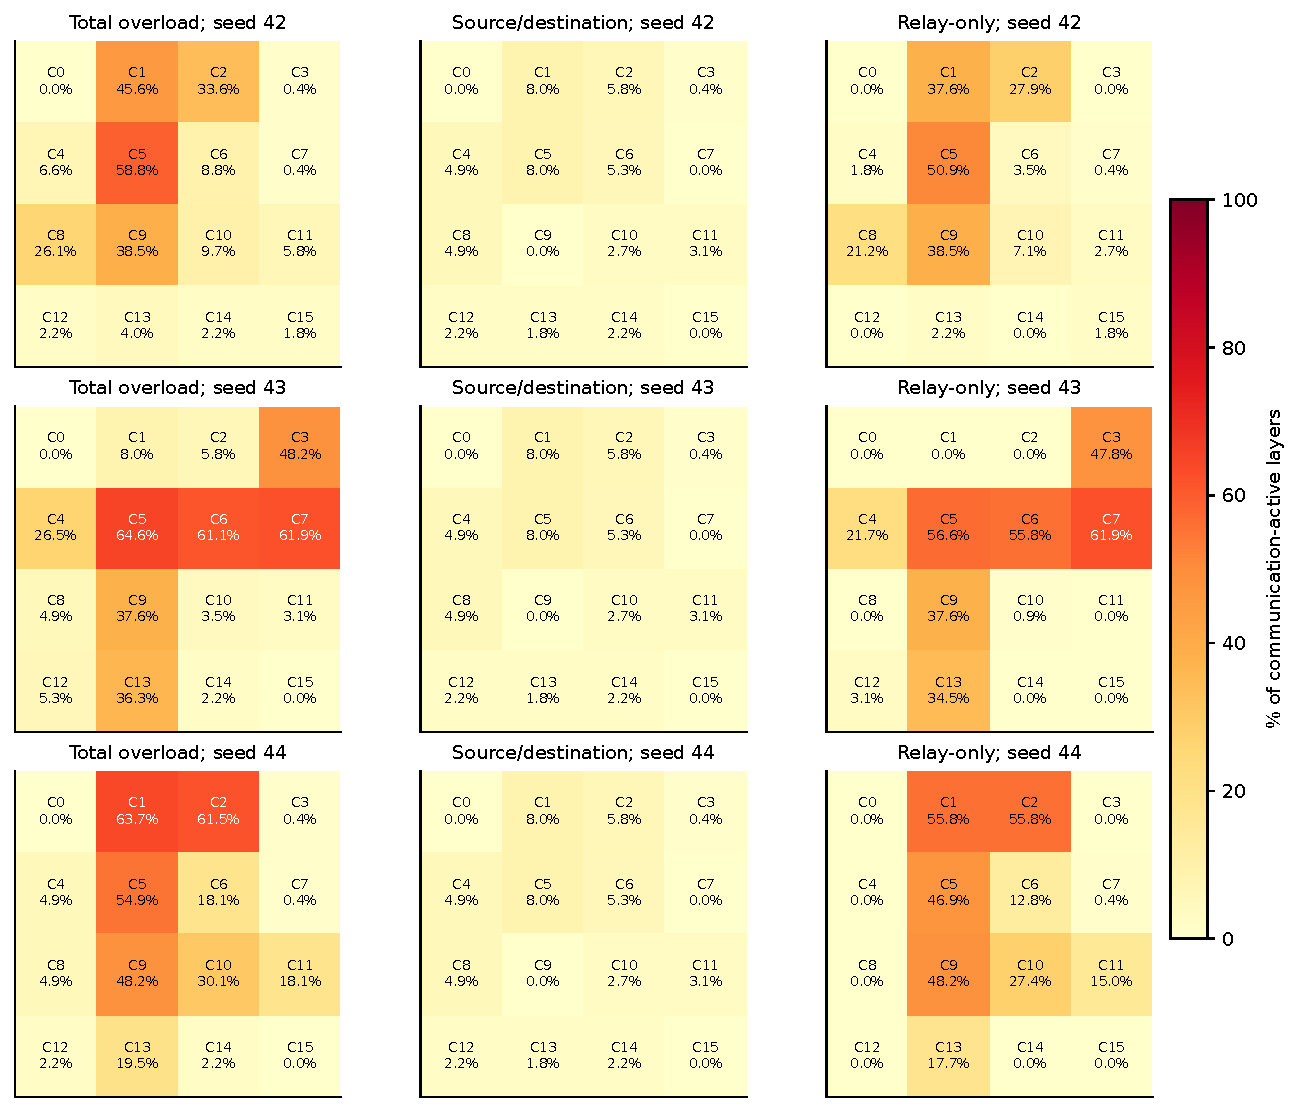
\includegraphics[width=.94\linewidth,height=.48\textheight,keepaspectratio]{figures/atlas/mesh_max_reliability_route_m3.pdf}\captionof{figure}{All three conceptual mapping seeds; common 0--100 percent colour scale.}\end{center}
\begin{center}{\scriptsize\setlength{\tabcolsep}{3pt}
\begin{tabular}{lrrrrrrrrr}
\toprule
Core & 42 Tot & 42 Own & 42 Rel & 43 Tot & 43 Own & 43 Rel & 44 Tot & 44 Own & 44 Rel \\
\midrule
0 & 0.000 & 0.000 & 0.000 & 0.000 & 0.000 & 0.000 & 0.000 & 0.000 & 0.000 \\
1 & 45.575 & 7.965 & 37.611 & 7.965 & 7.965 & 0.000 & 63.717 & 7.965 & 55.752 \\
2 & 33.628 & 5.752 & 27.876 & 5.752 & 5.752 & 0.000 & 61.504 & 5.752 & 55.752 \\
3 & 0.442 & 0.442 & 0.000 & 48.230 & 0.442 & 47.788 & 0.442 & 0.442 & 0.000 \\
4 & 6.637 & 4.867 & 1.770 & 26.549 & 4.867 & 21.681 & 4.867 & 4.867 & 0.000 \\
5 & 58.850 & 7.965 & 50.885 & 64.602 & 7.965 & 56.637 & 54.867 & 7.965 & 46.903 \\
6 & 8.850 & 5.310 & 3.540 & 61.062 & 5.310 & 55.752 & 18.142 & 5.310 & 12.832 \\
7 & 0.442 & 0.000 & 0.442 & 61.947 & 0.000 & 61.947 & 0.442 & 0.000 & 0.442 \\
8 & 26.106 & 4.867 & 21.239 & 4.867 & 4.867 & 0.000 & 4.867 & 4.867 & 0.000 \\
9 & 38.496 & 0.000 & 38.496 & 37.611 & 0.000 & 37.611 & 48.230 & 0.000 & 48.230 \\
10 & 9.735 & 2.655 & 7.080 & 3.540 & 2.655 & 0.885 & 30.088 & 2.655 & 27.434 \\
11 & 5.752 & 3.097 & 2.655 & 3.097 & 3.097 & 0.000 & 18.142 & 3.097 & 15.044 \\
12 & 2.212 & 2.212 & 0.000 & 5.310 & 2.212 & 3.097 & 2.212 & 2.212 & 0.000 \\
13 & 3.982 & 1.770 & 2.212 & 36.283 & 1.770 & 34.513 & 19.469 & 1.770 & 17.699 \\
14 & 2.212 & 2.212 & 0.000 & 2.212 & 2.212 & 0.000 & 2.212 & 2.212 & 0.000 \\
15 & 1.770 & 0.000 & 1.770 & 0.000 & 0.000 & 0.000 & 0.000 & 0.000 & 0.000 \\
\bottomrule\end{tabular}}
\captionof{table}{Exact heatmap percentages, with Tot = Own + Rel. Unrounded values are in the CSV.}
{\footnotesize\href{https://github.com/sanjeevkrishnaa/Compiler-Driven-ACE/blob/codex/ace-scheduler-correctness/docs/latex/qft96_final/data/heatmap_mesh_max_reliability_route_m3.csv}{Exact CSV values and sample counts}}
\end{center}
\clearpage\subsection*{Mesh max\_reliability; M=4; route counting}
\begin{center}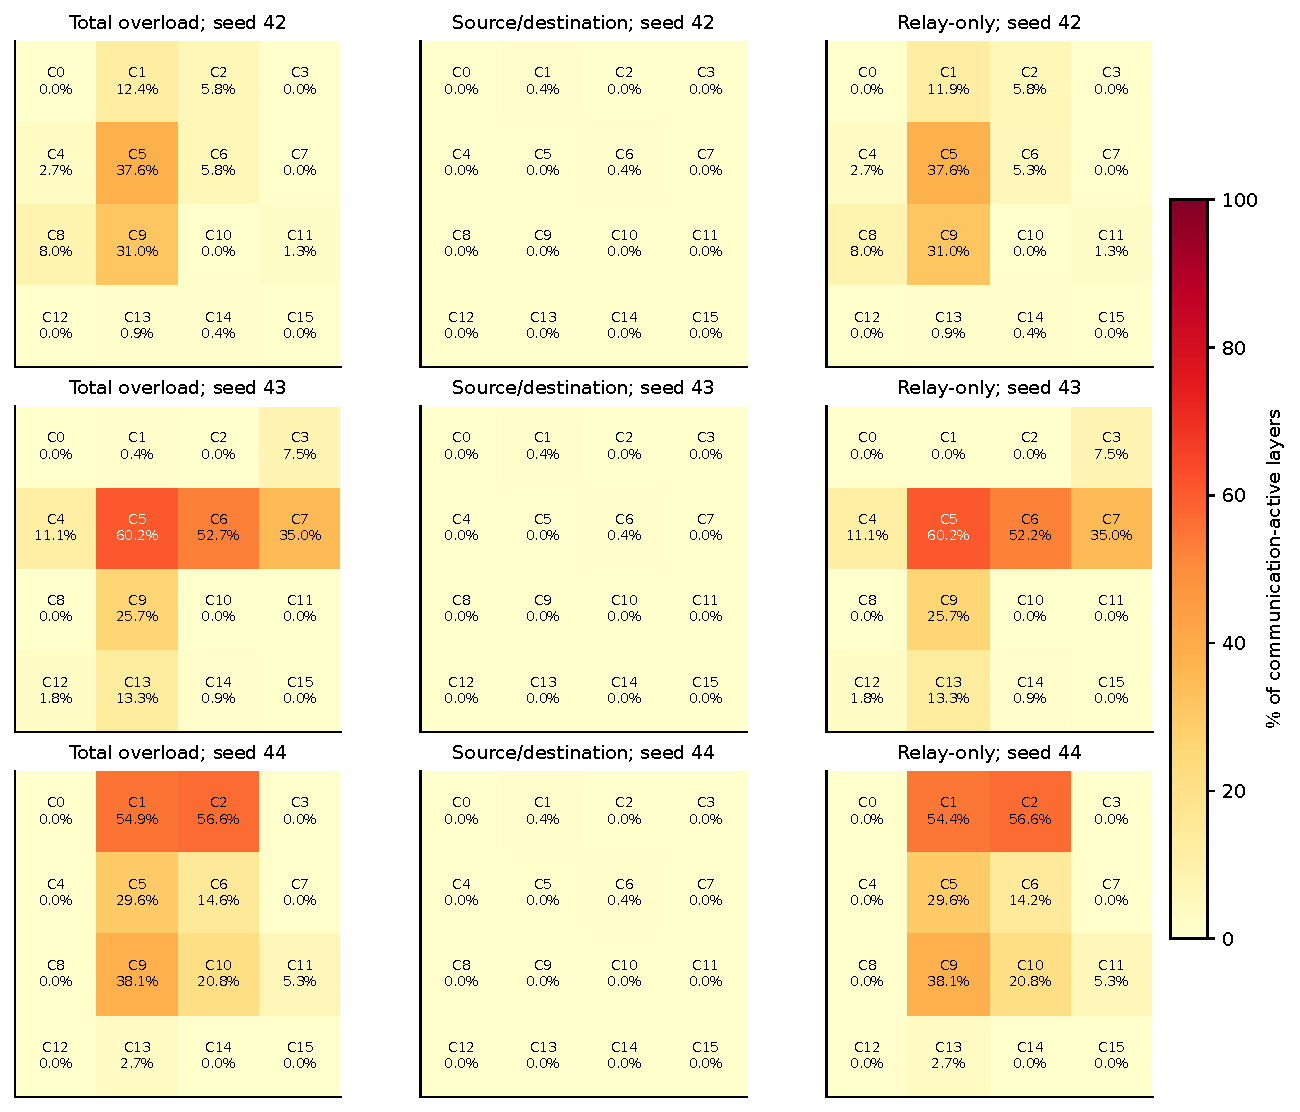
\includegraphics[width=.94\linewidth,height=.48\textheight,keepaspectratio]{figures/atlas/mesh_max_reliability_route_m4.pdf}\captionof{figure}{All three conceptual mapping seeds; common 0--100 percent colour scale.}\end{center}
\begin{center}{\scriptsize\setlength{\tabcolsep}{3pt}
\begin{tabular}{lrrrrrrrrr}
\toprule
Core & 42 Tot & 42 Own & 42 Rel & 43 Tot & 43 Own & 43 Rel & 44 Tot & 44 Own & 44 Rel \\
\midrule
0 & 0.000 & 0.000 & 0.000 & 0.000 & 0.000 & 0.000 & 0.000 & 0.000 & 0.000 \\
1 & 12.389 & 0.442 & 11.947 & 0.442 & 0.442 & 0.000 & 54.867 & 0.442 & 54.425 \\
2 & 5.752 & 0.000 & 5.752 & 0.000 & 0.000 & 0.000 & 56.637 & 0.000 & 56.637 \\
3 & 0.000 & 0.000 & 0.000 & 7.522 & 0.000 & 7.522 & 0.000 & 0.000 & 0.000 \\
4 & 2.655 & 0.000 & 2.655 & 11.062 & 0.000 & 11.062 & 0.000 & 0.000 & 0.000 \\
5 & 37.611 & 0.000 & 37.611 & 60.177 & 0.000 & 60.177 & 29.646 & 0.000 & 29.646 \\
6 & 5.752 & 0.442 & 5.310 & 52.655 & 0.442 & 52.212 & 14.602 & 0.442 & 14.159 \\
7 & 0.000 & 0.000 & 0.000 & 34.956 & 0.000 & 34.956 & 0.000 & 0.000 & 0.000 \\
8 & 7.965 & 0.000 & 7.965 & 0.000 & 0.000 & 0.000 & 0.000 & 0.000 & 0.000 \\
9 & 30.973 & 0.000 & 30.973 & 25.664 & 0.000 & 25.664 & 38.053 & 0.000 & 38.053 \\
10 & 0.000 & 0.000 & 0.000 & 0.000 & 0.000 & 0.000 & 20.796 & 0.000 & 20.796 \\
11 & 1.327 & 0.000 & 1.327 & 0.000 & 0.000 & 0.000 & 5.310 & 0.000 & 5.310 \\
12 & 0.000 & 0.000 & 0.000 & 1.770 & 0.000 & 1.770 & 0.000 & 0.000 & 0.000 \\
13 & 0.885 & 0.000 & 0.885 & 13.274 & 0.000 & 13.274 & 2.655 & 0.000 & 2.655 \\
14 & 0.442 & 0.000 & 0.442 & 0.885 & 0.000 & 0.885 & 0.000 & 0.000 & 0.000 \\
15 & 0.000 & 0.000 & 0.000 & 0.000 & 0.000 & 0.000 & 0.000 & 0.000 & 0.000 \\
\bottomrule\end{tabular}}
\captionof{table}{Exact heatmap percentages, with Tot = Own + Rel. Unrounded values are in the CSV.}
{\footnotesize\href{https://github.com/sanjeevkrishnaa/Compiler-Driven-ACE/blob/codex/ace-scheduler-correctness/docs/latex/qft96_final/data/heatmap_mesh_max_reliability_route_m4.csv}{Exact CSV values and sample counts}}
\end{center}
\clearpage\subsection*{Mesh max\_reliability; M=6; route counting}
\begin{center}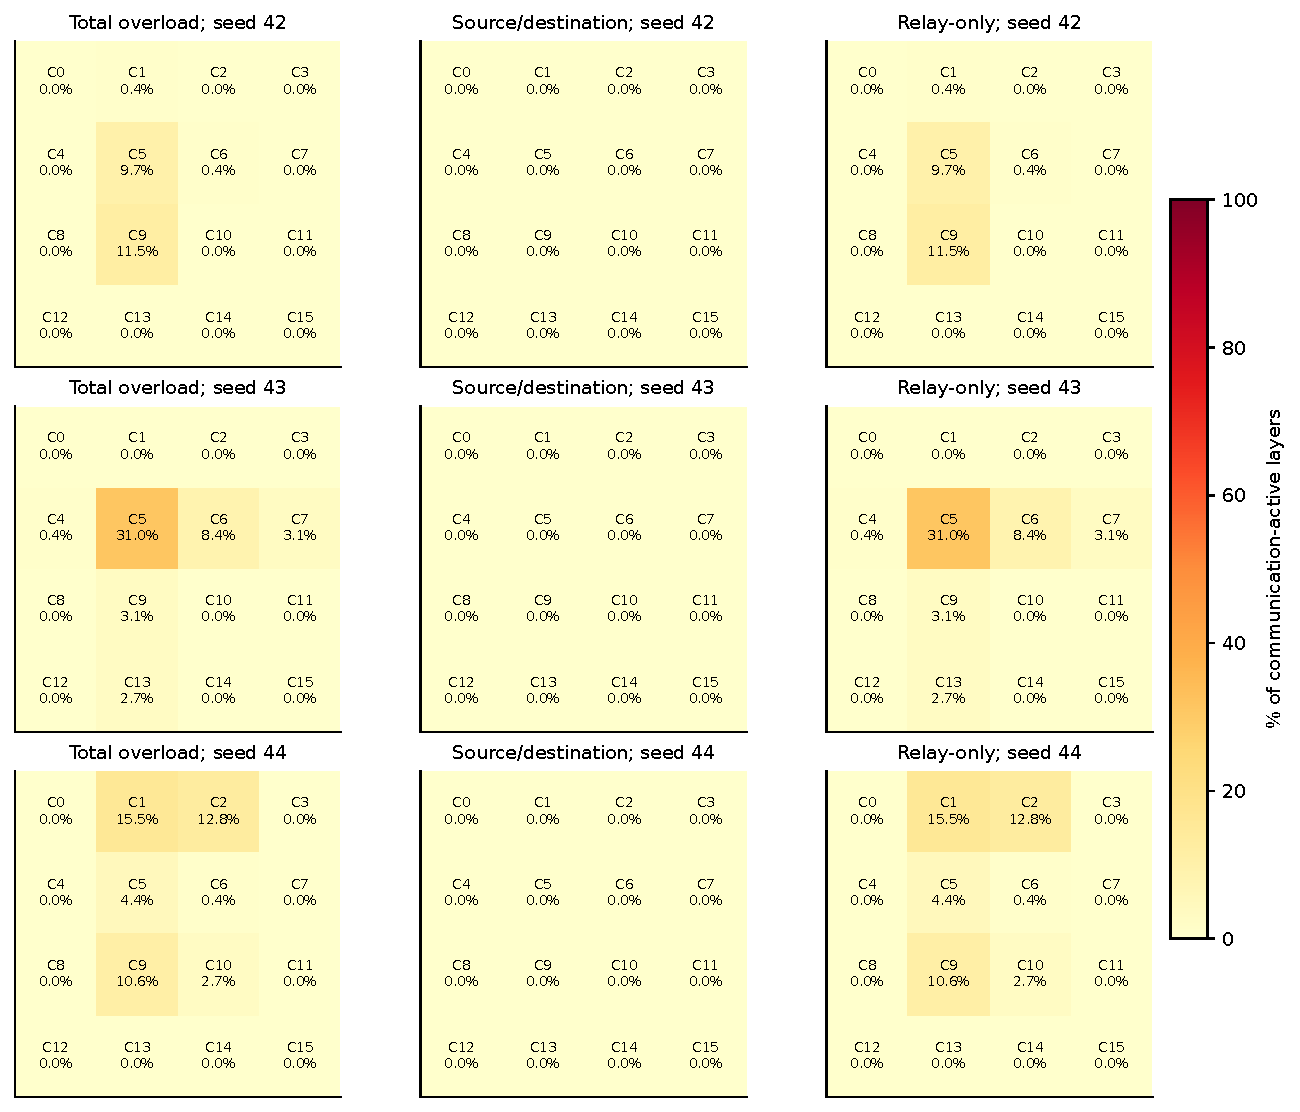
\includegraphics[width=.94\linewidth,height=.48\textheight,keepaspectratio]{figures/atlas/mesh_max_reliability_route_m6.pdf}\captionof{figure}{All three conceptual mapping seeds; common 0--100 percent colour scale.}\end{center}
\begin{center}{\scriptsize\setlength{\tabcolsep}{3pt}
\begin{tabular}{lrrrrrrrrr}
\toprule
Core & 42 Tot & 42 Own & 42 Rel & 43 Tot & 43 Own & 43 Rel & 44 Tot & 44 Own & 44 Rel \\
\midrule
0 & 0.000 & 0.000 & 0.000 & 0.000 & 0.000 & 0.000 & 0.000 & 0.000 & 0.000 \\
1 & 0.442 & 0.000 & 0.442 & 0.000 & 0.000 & 0.000 & 15.487 & 0.000 & 15.487 \\
2 & 0.000 & 0.000 & 0.000 & 0.000 & 0.000 & 0.000 & 12.832 & 0.000 & 12.832 \\
3 & 0.000 & 0.000 & 0.000 & 0.000 & 0.000 & 0.000 & 0.000 & 0.000 & 0.000 \\
4 & 0.000 & 0.000 & 0.000 & 0.442 & 0.000 & 0.442 & 0.000 & 0.000 & 0.000 \\
5 & 9.735 & 0.000 & 9.735 & 30.973 & 0.000 & 30.973 & 4.425 & 0.000 & 4.425 \\
6 & 0.442 & 0.000 & 0.442 & 8.407 & 0.000 & 8.407 & 0.442 & 0.000 & 0.442 \\
7 & 0.000 & 0.000 & 0.000 & 3.097 & 0.000 & 3.097 & 0.000 & 0.000 & 0.000 \\
8 & 0.000 & 0.000 & 0.000 & 0.000 & 0.000 & 0.000 & 0.000 & 0.000 & 0.000 \\
9 & 11.504 & 0.000 & 11.504 & 3.097 & 0.000 & 3.097 & 10.619 & 0.000 & 10.619 \\
10 & 0.000 & 0.000 & 0.000 & 0.000 & 0.000 & 0.000 & 2.655 & 0.000 & 2.655 \\
11 & 0.000 & 0.000 & 0.000 & 0.000 & 0.000 & 0.000 & 0.000 & 0.000 & 0.000 \\
12 & 0.000 & 0.000 & 0.000 & 0.000 & 0.000 & 0.000 & 0.000 & 0.000 & 0.000 \\
13 & 0.000 & 0.000 & 0.000 & 2.655 & 0.000 & 2.655 & 0.000 & 0.000 & 0.000 \\
14 & 0.000 & 0.000 & 0.000 & 0.000 & 0.000 & 0.000 & 0.000 & 0.000 & 0.000 \\
15 & 0.000 & 0.000 & 0.000 & 0.000 & 0.000 & 0.000 & 0.000 & 0.000 & 0.000 \\
\bottomrule\end{tabular}}
\captionof{table}{Exact heatmap percentages, with Tot = Own + Rel. Unrounded values are in the CSV.}
{\footnotesize\href{https://github.com/sanjeevkrishnaa/Compiler-Driven-ACE/blob/codex/ace-scheduler-correctness/docs/latex/qft96_final/data/heatmap_mesh_max_reliability_route_m6.csv}{Exact CSV values and sample counts}}
\end{center}
\clearpage\subsection*{Mesh max\_reliability; M=8; route counting}
\begin{center}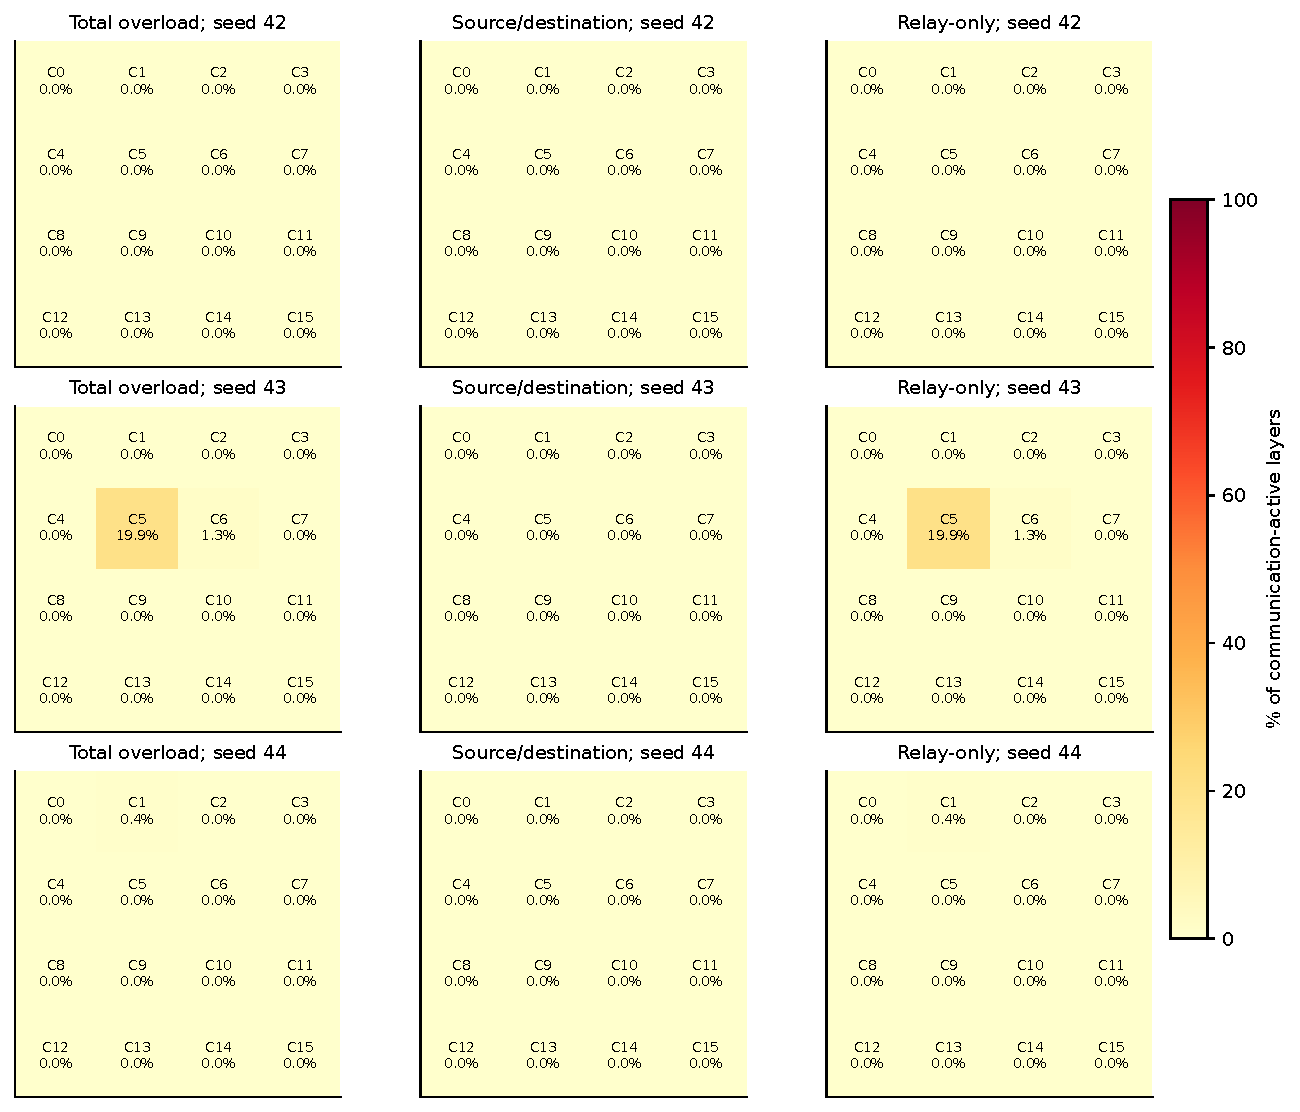
\includegraphics[width=.94\linewidth,height=.48\textheight,keepaspectratio]{figures/atlas/mesh_max_reliability_route_m8.pdf}\captionof{figure}{All three conceptual mapping seeds; common 0--100 percent colour scale.}\end{center}
\begin{center}{\scriptsize\setlength{\tabcolsep}{3pt}
\begin{tabular}{lrrrrrrrrr}
\toprule
Core & 42 Tot & 42 Own & 42 Rel & 43 Tot & 43 Own & 43 Rel & 44 Tot & 44 Own & 44 Rel \\
\midrule
0 & 0.000 & 0.000 & 0.000 & 0.000 & 0.000 & 0.000 & 0.000 & 0.000 & 0.000 \\
1 & 0.000 & 0.000 & 0.000 & 0.000 & 0.000 & 0.000 & 0.442 & 0.000 & 0.442 \\
2 & 0.000 & 0.000 & 0.000 & 0.000 & 0.000 & 0.000 & 0.000 & 0.000 & 0.000 \\
3 & 0.000 & 0.000 & 0.000 & 0.000 & 0.000 & 0.000 & 0.000 & 0.000 & 0.000 \\
4 & 0.000 & 0.000 & 0.000 & 0.000 & 0.000 & 0.000 & 0.000 & 0.000 & 0.000 \\
5 & 0.000 & 0.000 & 0.000 & 19.912 & 0.000 & 19.912 & 0.000 & 0.000 & 0.000 \\
6 & 0.000 & 0.000 & 0.000 & 1.327 & 0.000 & 1.327 & 0.000 & 0.000 & 0.000 \\
7 & 0.000 & 0.000 & 0.000 & 0.000 & 0.000 & 0.000 & 0.000 & 0.000 & 0.000 \\
8 & 0.000 & 0.000 & 0.000 & 0.000 & 0.000 & 0.000 & 0.000 & 0.000 & 0.000 \\
9 & 0.000 & 0.000 & 0.000 & 0.000 & 0.000 & 0.000 & 0.000 & 0.000 & 0.000 \\
10 & 0.000 & 0.000 & 0.000 & 0.000 & 0.000 & 0.000 & 0.000 & 0.000 & 0.000 \\
11 & 0.000 & 0.000 & 0.000 & 0.000 & 0.000 & 0.000 & 0.000 & 0.000 & 0.000 \\
12 & 0.000 & 0.000 & 0.000 & 0.000 & 0.000 & 0.000 & 0.000 & 0.000 & 0.000 \\
13 & 0.000 & 0.000 & 0.000 & 0.000 & 0.000 & 0.000 & 0.000 & 0.000 & 0.000 \\
14 & 0.000 & 0.000 & 0.000 & 0.000 & 0.000 & 0.000 & 0.000 & 0.000 & 0.000 \\
15 & 0.000 & 0.000 & 0.000 & 0.000 & 0.000 & 0.000 & 0.000 & 0.000 & 0.000 \\
\bottomrule\end{tabular}}
\captionof{table}{Exact heatmap percentages, with Tot = Own + Rel. Unrounded values are in the CSV.}
{\footnotesize\href{https://github.com/sanjeevkrishnaa/Compiler-Driven-ACE/blob/codex/ace-scheduler-correctness/docs/latex/qft96_final/data/heatmap_mesh_max_reliability_route_m8.csv}{Exact CSV values and sample counts}}
\end{center}
\clearpage\subsection*{Mesh max\_reliability; M=16; route counting}
\begin{center}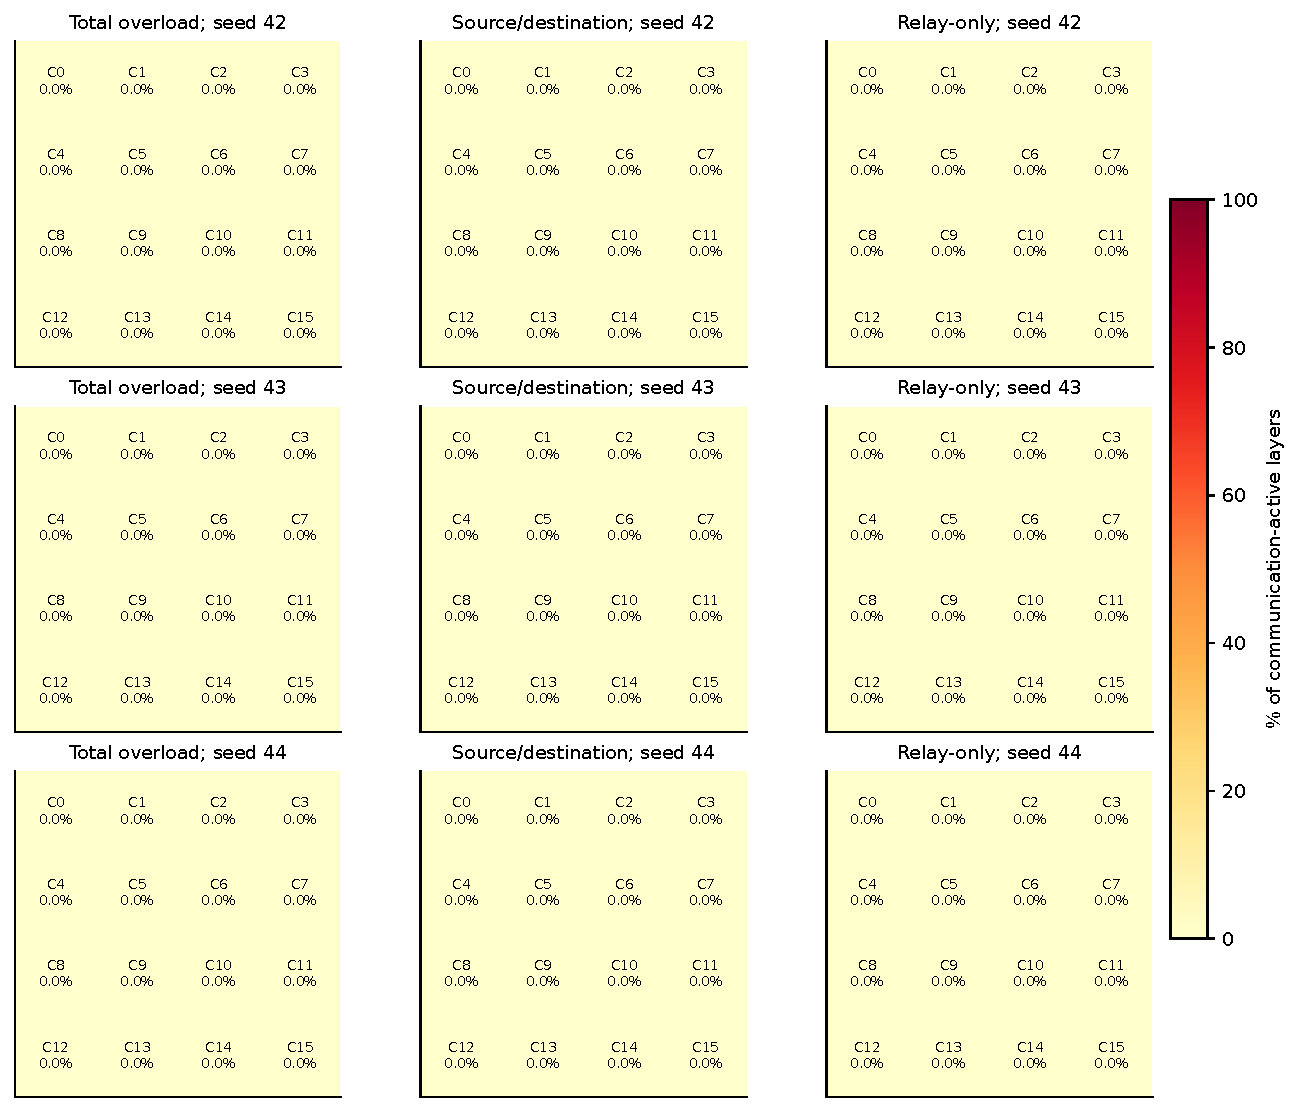
\includegraphics[width=.94\linewidth,height=.48\textheight,keepaspectratio]{figures/atlas/mesh_max_reliability_route_m16.pdf}\captionof{figure}{All three conceptual mapping seeds; common 0--100 percent colour scale.}\end{center}
\begin{center}{\scriptsize\setlength{\tabcolsep}{3pt}
\begin{tabular}{lrrrrrrrrr}
\toprule
Core & 42 Tot & 42 Own & 42 Rel & 43 Tot & 43 Own & 43 Rel & 44 Tot & 44 Own & 44 Rel \\
\midrule
0 & 0.000 & 0.000 & 0.000 & 0.000 & 0.000 & 0.000 & 0.000 & 0.000 & 0.000 \\
1 & 0.000 & 0.000 & 0.000 & 0.000 & 0.000 & 0.000 & 0.000 & 0.000 & 0.000 \\
2 & 0.000 & 0.000 & 0.000 & 0.000 & 0.000 & 0.000 & 0.000 & 0.000 & 0.000 \\
3 & 0.000 & 0.000 & 0.000 & 0.000 & 0.000 & 0.000 & 0.000 & 0.000 & 0.000 \\
4 & 0.000 & 0.000 & 0.000 & 0.000 & 0.000 & 0.000 & 0.000 & 0.000 & 0.000 \\
5 & 0.000 & 0.000 & 0.000 & 0.000 & 0.000 & 0.000 & 0.000 & 0.000 & 0.000 \\
6 & 0.000 & 0.000 & 0.000 & 0.000 & 0.000 & 0.000 & 0.000 & 0.000 & 0.000 \\
7 & 0.000 & 0.000 & 0.000 & 0.000 & 0.000 & 0.000 & 0.000 & 0.000 & 0.000 \\
8 & 0.000 & 0.000 & 0.000 & 0.000 & 0.000 & 0.000 & 0.000 & 0.000 & 0.000 \\
9 & 0.000 & 0.000 & 0.000 & 0.000 & 0.000 & 0.000 & 0.000 & 0.000 & 0.000 \\
10 & 0.000 & 0.000 & 0.000 & 0.000 & 0.000 & 0.000 & 0.000 & 0.000 & 0.000 \\
11 & 0.000 & 0.000 & 0.000 & 0.000 & 0.000 & 0.000 & 0.000 & 0.000 & 0.000 \\
12 & 0.000 & 0.000 & 0.000 & 0.000 & 0.000 & 0.000 & 0.000 & 0.000 & 0.000 \\
13 & 0.000 & 0.000 & 0.000 & 0.000 & 0.000 & 0.000 & 0.000 & 0.000 & 0.000 \\
14 & 0.000 & 0.000 & 0.000 & 0.000 & 0.000 & 0.000 & 0.000 & 0.000 & 0.000 \\
15 & 0.000 & 0.000 & 0.000 & 0.000 & 0.000 & 0.000 & 0.000 & 0.000 & 0.000 \\
\bottomrule\end{tabular}}
\captionof{table}{Exact heatmap percentages, with Tot = Own + Rel. Unrounded values are in the CSV.}
{\footnotesize\href{https://github.com/sanjeevkrishnaa/Compiler-Driven-ACE/blob/codex/ace-scheduler-correctness/docs/latex/qft96_final/data/heatmap_mesh_max_reliability_route_m16.csv}{Exact CSV values and sample counts}}
\end{center}
\clearpage\subsection*{Mesh max\_reliability; M=32; route counting}
\begin{center}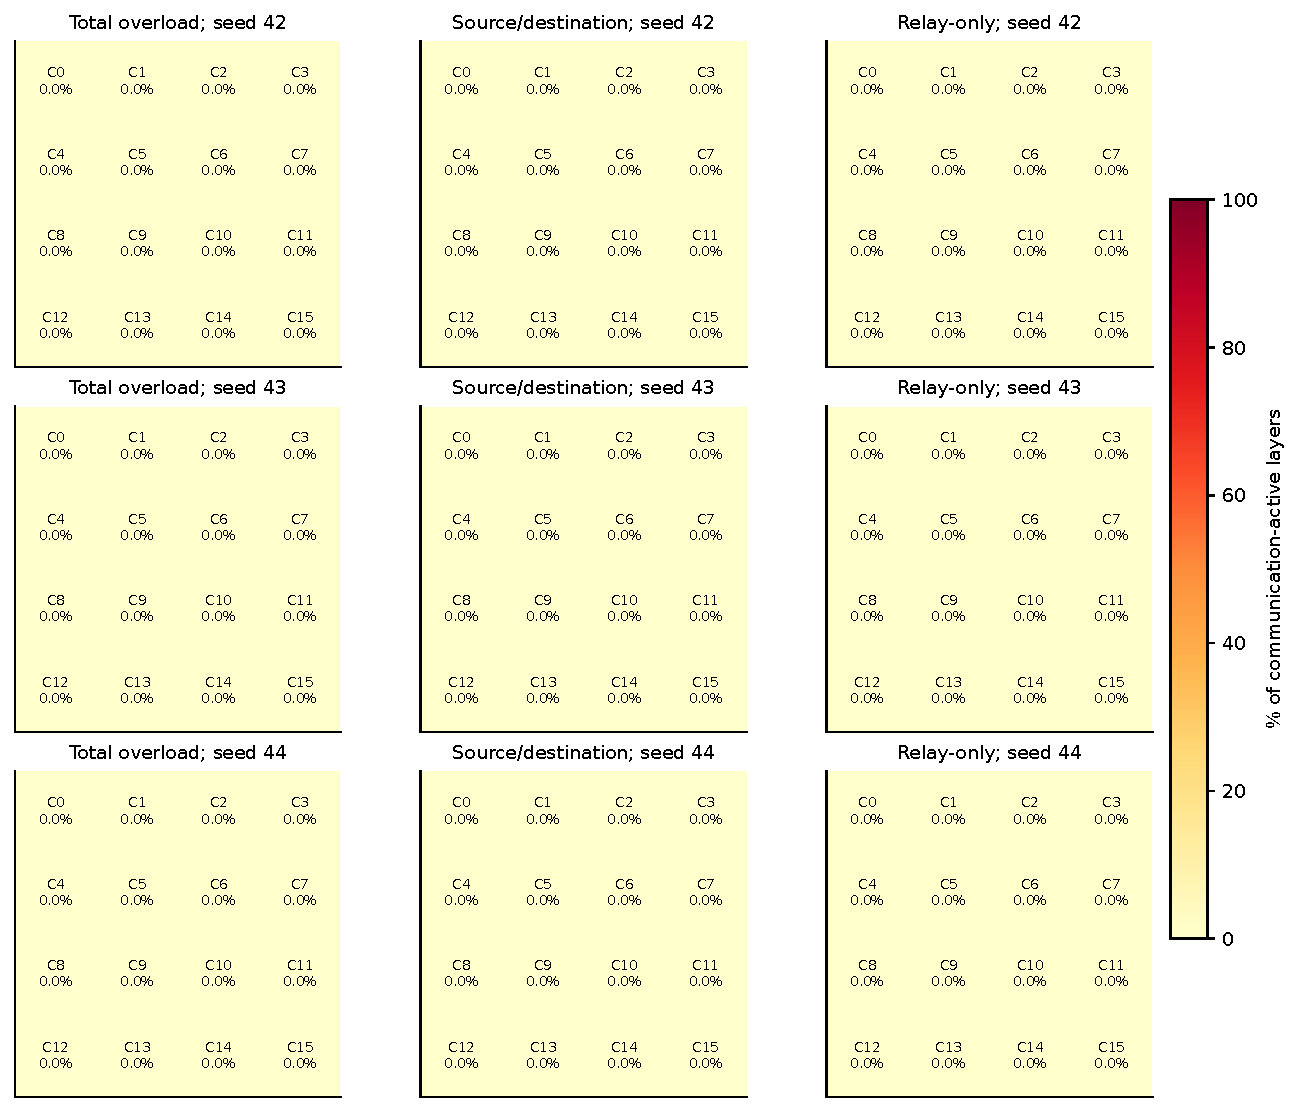
\includegraphics[width=.94\linewidth,height=.48\textheight,keepaspectratio]{figures/atlas/mesh_max_reliability_route_m32.pdf}\captionof{figure}{All three conceptual mapping seeds; common 0--100 percent colour scale.}\end{center}
\begin{center}{\scriptsize\setlength{\tabcolsep}{3pt}
\begin{tabular}{lrrrrrrrrr}
\toprule
Core & 42 Tot & 42 Own & 42 Rel & 43 Tot & 43 Own & 43 Rel & 44 Tot & 44 Own & 44 Rel \\
\midrule
0 & 0.000 & 0.000 & 0.000 & 0.000 & 0.000 & 0.000 & 0.000 & 0.000 & 0.000 \\
1 & 0.000 & 0.000 & 0.000 & 0.000 & 0.000 & 0.000 & 0.000 & 0.000 & 0.000 \\
2 & 0.000 & 0.000 & 0.000 & 0.000 & 0.000 & 0.000 & 0.000 & 0.000 & 0.000 \\
3 & 0.000 & 0.000 & 0.000 & 0.000 & 0.000 & 0.000 & 0.000 & 0.000 & 0.000 \\
4 & 0.000 & 0.000 & 0.000 & 0.000 & 0.000 & 0.000 & 0.000 & 0.000 & 0.000 \\
5 & 0.000 & 0.000 & 0.000 & 0.000 & 0.000 & 0.000 & 0.000 & 0.000 & 0.000 \\
6 & 0.000 & 0.000 & 0.000 & 0.000 & 0.000 & 0.000 & 0.000 & 0.000 & 0.000 \\
7 & 0.000 & 0.000 & 0.000 & 0.000 & 0.000 & 0.000 & 0.000 & 0.000 & 0.000 \\
8 & 0.000 & 0.000 & 0.000 & 0.000 & 0.000 & 0.000 & 0.000 & 0.000 & 0.000 \\
9 & 0.000 & 0.000 & 0.000 & 0.000 & 0.000 & 0.000 & 0.000 & 0.000 & 0.000 \\
10 & 0.000 & 0.000 & 0.000 & 0.000 & 0.000 & 0.000 & 0.000 & 0.000 & 0.000 \\
11 & 0.000 & 0.000 & 0.000 & 0.000 & 0.000 & 0.000 & 0.000 & 0.000 & 0.000 \\
12 & 0.000 & 0.000 & 0.000 & 0.000 & 0.000 & 0.000 & 0.000 & 0.000 & 0.000 \\
13 & 0.000 & 0.000 & 0.000 & 0.000 & 0.000 & 0.000 & 0.000 & 0.000 & 0.000 \\
14 & 0.000 & 0.000 & 0.000 & 0.000 & 0.000 & 0.000 & 0.000 & 0.000 & 0.000 \\
15 & 0.000 & 0.000 & 0.000 & 0.000 & 0.000 & 0.000 & 0.000 & 0.000 & 0.000 \\
\bottomrule\end{tabular}}
\captionof{table}{Exact heatmap percentages, with Tot = Own + Rel. Unrounded values are in the CSV.}
{\footnotesize\href{https://github.com/sanjeevkrishnaa/Compiler-Driven-ACE/blob/codex/ace-scheduler-correctness/docs/latex/qft96_final/data/heatmap_mesh_max_reliability_route_m32.csv}{Exact CSV values and sample counts}}
\end{center}
\clearpage\subsection*{Mesh max\_reliability; M=2; hop counting}
\begin{center}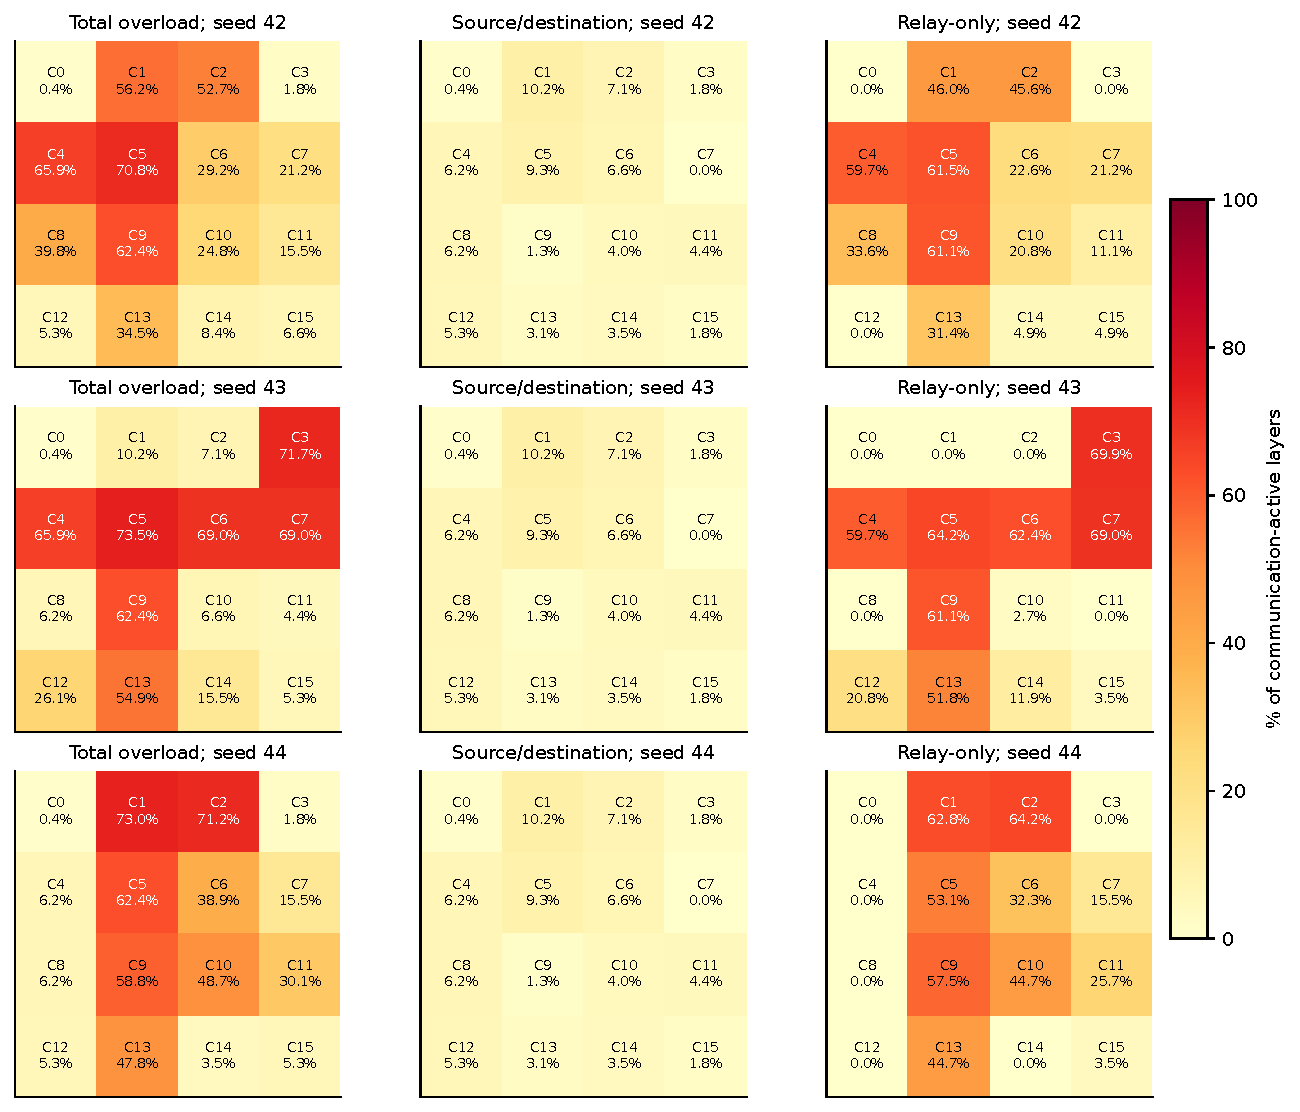
\includegraphics[width=.94\linewidth,height=.48\textheight,keepaspectratio]{figures/atlas/mesh_max_reliability_hop_m2.pdf}\captionof{figure}{All three conceptual mapping seeds; common 0--100 percent colour scale.}\end{center}
\begin{center}{\scriptsize\setlength{\tabcolsep}{3pt}
\begin{tabular}{lrrrrrrrrr}
\toprule
Core & 42 Tot & 42 Own & 42 Rel & 43 Tot & 43 Own & 43 Rel & 44 Tot & 44 Own & 44 Rel \\
\midrule
0 & 0.442 & 0.442 & 0.000 & 0.442 & 0.442 & 0.000 & 0.442 & 0.442 & 0.000 \\
1 & 56.195 & 10.177 & 46.018 & 10.177 & 10.177 & 0.000 & 73.009 & 10.177 & 62.832 \\
2 & 52.655 & 7.080 & 45.575 & 7.080 & 7.080 & 0.000 & 71.239 & 7.080 & 64.159 \\
3 & 1.770 & 1.770 & 0.000 & 71.681 & 1.770 & 69.912 & 1.770 & 1.770 & 0.000 \\
4 & 65.929 & 6.195 & 59.735 & 65.929 & 6.195 & 59.735 & 6.195 & 6.195 & 0.000 \\
5 & 70.796 & 9.292 & 61.504 & 73.451 & 9.292 & 64.159 & 62.389 & 9.292 & 53.097 \\
6 & 29.204 & 6.637 & 22.566 & 69.027 & 6.637 & 62.389 & 38.938 & 6.637 & 32.301 \\
7 & 21.239 & 0.000 & 21.239 & 69.027 & 0.000 & 69.027 & 15.487 & 0.000 & 15.487 \\
8 & 39.823 & 6.195 & 33.628 & 6.195 & 6.195 & 0.000 & 6.195 & 6.195 & 0.000 \\
9 & 62.389 & 1.327 & 61.062 & 62.389 & 1.327 & 61.062 & 58.850 & 1.327 & 57.522 \\
10 & 24.779 & 3.982 & 20.796 & 6.637 & 3.982 & 2.655 & 48.673 & 3.982 & 44.690 \\
11 & 15.487 & 4.425 & 11.062 & 4.425 & 4.425 & 0.000 & 30.088 & 4.425 & 25.664 \\
12 & 5.310 & 5.310 & 0.000 & 26.106 & 5.310 & 20.796 & 5.310 & 5.310 & 0.000 \\
13 & 34.513 & 3.097 & 31.416 & 54.867 & 3.097 & 51.770 & 47.788 & 3.097 & 44.690 \\
14 & 8.407 & 3.540 & 4.867 & 15.487 & 3.540 & 11.947 & 3.540 & 3.540 & 0.000 \\
15 & 6.637 & 1.770 & 4.867 & 5.310 & 1.770 & 3.540 & 5.310 & 1.770 & 3.540 \\
\bottomrule\end{tabular}}
\captionof{table}{Exact heatmap percentages, with Tot = Own + Rel. Unrounded values are in the CSV.}
{\footnotesize\href{https://github.com/sanjeevkrishnaa/Compiler-Driven-ACE/blob/codex/ace-scheduler-correctness/docs/latex/qft96_final/data/heatmap_mesh_max_reliability_hop_m2.csv}{Exact CSV values and sample counts}}
\end{center}
\clearpage\subsection*{Mesh max\_reliability; M=3; hop counting}
\begin{center}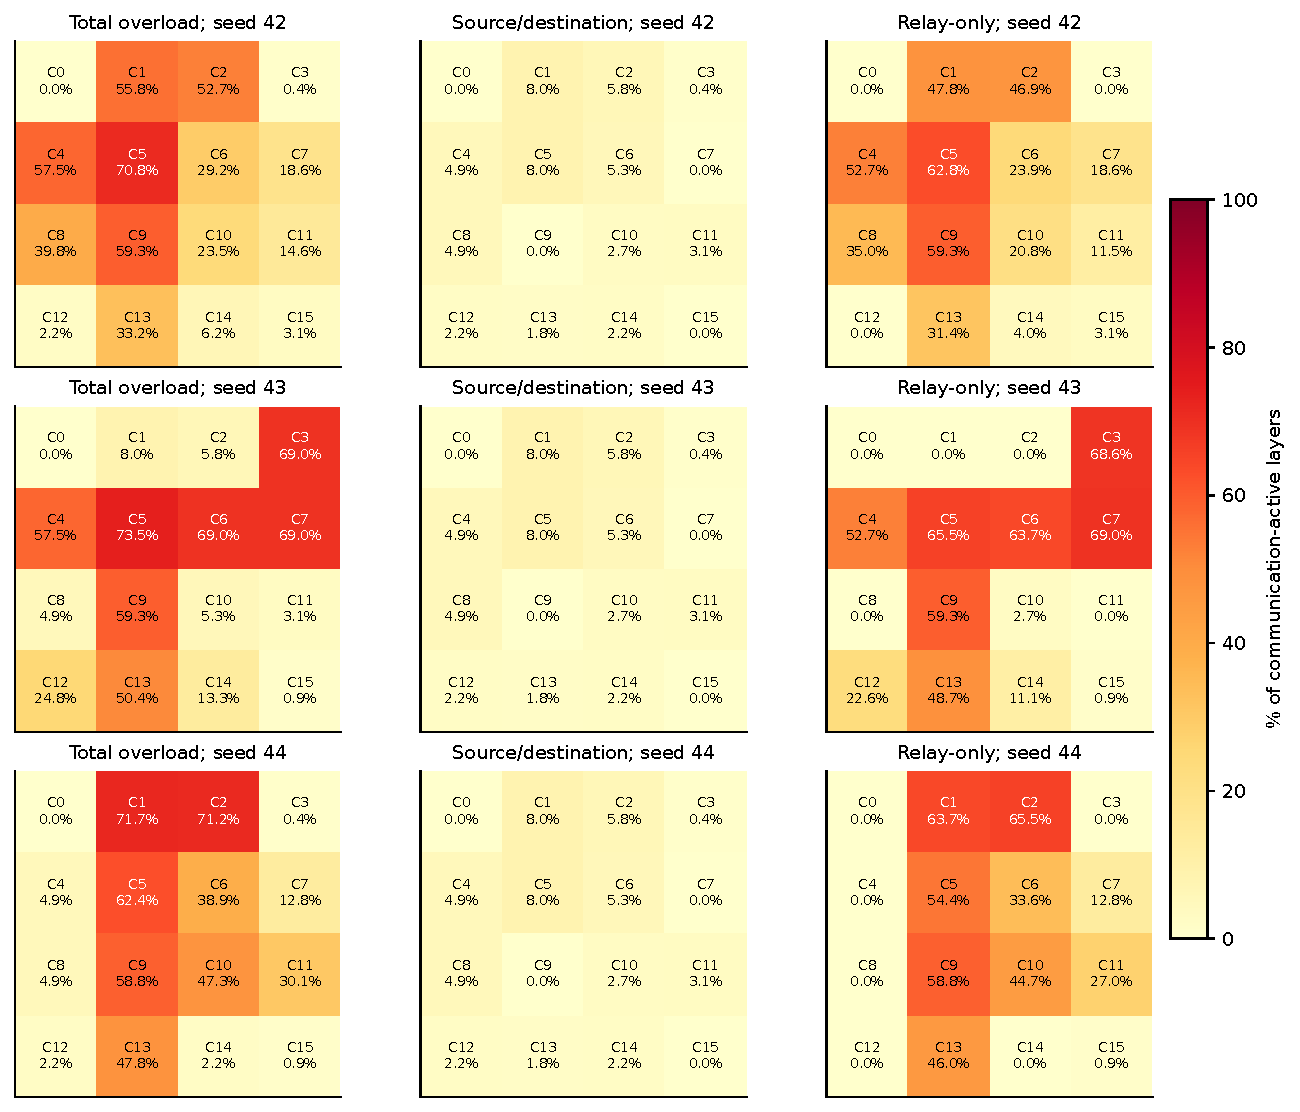
\includegraphics[width=.94\linewidth,height=.48\textheight,keepaspectratio]{figures/atlas/mesh_max_reliability_hop_m3.pdf}\captionof{figure}{All three conceptual mapping seeds; common 0--100 percent colour scale.}\end{center}
\begin{center}{\scriptsize\setlength{\tabcolsep}{3pt}
\begin{tabular}{lrrrrrrrrr}
\toprule
Core & 42 Tot & 42 Own & 42 Rel & 43 Tot & 43 Own & 43 Rel & 44 Tot & 44 Own & 44 Rel \\
\midrule
0 & 0.000 & 0.000 & 0.000 & 0.000 & 0.000 & 0.000 & 0.000 & 0.000 & 0.000 \\
1 & 55.752 & 7.965 & 47.788 & 7.965 & 7.965 & 0.000 & 71.681 & 7.965 & 63.717 \\
2 & 52.655 & 5.752 & 46.903 & 5.752 & 5.752 & 0.000 & 71.239 & 5.752 & 65.487 \\
3 & 0.442 & 0.442 & 0.000 & 69.027 & 0.442 & 68.584 & 0.442 & 0.442 & 0.000 \\
4 & 57.522 & 4.867 & 52.655 & 57.522 & 4.867 & 52.655 & 4.867 & 4.867 & 0.000 \\
5 & 70.796 & 7.965 & 62.832 & 73.451 & 7.965 & 65.487 & 62.389 & 7.965 & 54.425 \\
6 & 29.204 & 5.310 & 23.894 & 69.027 & 5.310 & 63.717 & 38.938 & 5.310 & 33.628 \\
7 & 18.584 & 0.000 & 18.584 & 69.027 & 0.000 & 69.027 & 12.832 & 0.000 & 12.832 \\
8 & 39.823 & 4.867 & 34.956 & 4.867 & 4.867 & 0.000 & 4.867 & 4.867 & 0.000 \\
9 & 59.292 & 0.000 & 59.292 & 59.292 & 0.000 & 59.292 & 58.850 & 0.000 & 58.850 \\
10 & 23.451 & 2.655 & 20.796 & 5.310 & 2.655 & 2.655 & 47.345 & 2.655 & 44.690 \\
11 & 14.602 & 3.097 & 11.504 & 3.097 & 3.097 & 0.000 & 30.088 & 3.097 & 26.991 \\
12 & 2.212 & 2.212 & 0.000 & 24.779 & 2.212 & 22.566 & 2.212 & 2.212 & 0.000 \\
13 & 33.186 & 1.770 & 31.416 & 50.442 & 1.770 & 48.673 & 47.788 & 1.770 & 46.018 \\
14 & 6.195 & 2.212 & 3.982 & 13.274 & 2.212 & 11.062 & 2.212 & 2.212 & 0.000 \\
15 & 3.097 & 0.000 & 3.097 & 0.885 & 0.000 & 0.885 & 0.885 & 0.000 & 0.885 \\
\bottomrule\end{tabular}}
\captionof{table}{Exact heatmap percentages, with Tot = Own + Rel. Unrounded values are in the CSV.}
{\footnotesize\href{https://github.com/sanjeevkrishnaa/Compiler-Driven-ACE/blob/codex/ace-scheduler-correctness/docs/latex/qft96_final/data/heatmap_mesh_max_reliability_hop_m3.csv}{Exact CSV values and sample counts}}
\end{center}
\clearpage\subsection*{Mesh max\_reliability; M=4; hop counting}
\begin{center}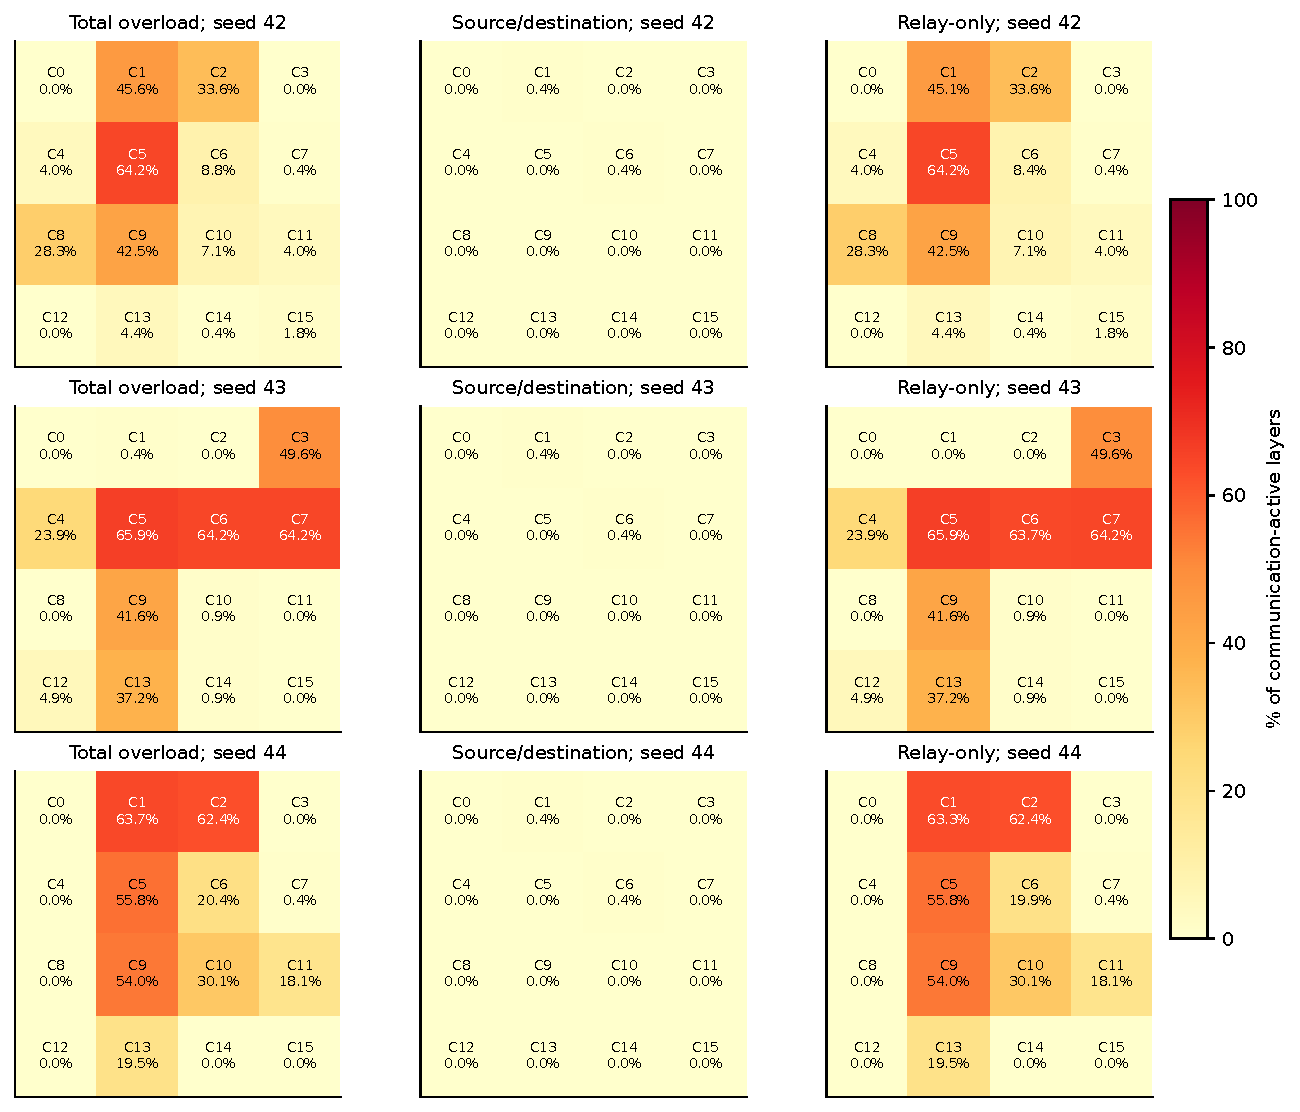
\includegraphics[width=.94\linewidth,height=.48\textheight,keepaspectratio]{figures/atlas/mesh_max_reliability_hop_m4.pdf}\captionof{figure}{All three conceptual mapping seeds; common 0--100 percent colour scale.}\end{center}
\begin{center}{\scriptsize\setlength{\tabcolsep}{3pt}
\begin{tabular}{lrrrrrrrrr}
\toprule
Core & 42 Tot & 42 Own & 42 Rel & 43 Tot & 43 Own & 43 Rel & 44 Tot & 44 Own & 44 Rel \\
\midrule
0 & 0.000 & 0.000 & 0.000 & 0.000 & 0.000 & 0.000 & 0.000 & 0.000 & 0.000 \\
1 & 45.575 & 0.442 & 45.133 & 0.442 & 0.442 & 0.000 & 63.717 & 0.442 & 63.274 \\
2 & 33.628 & 0.000 & 33.628 & 0.000 & 0.000 & 0.000 & 62.389 & 0.000 & 62.389 \\
3 & 0.000 & 0.000 & 0.000 & 49.558 & 0.000 & 49.558 & 0.000 & 0.000 & 0.000 \\
4 & 3.982 & 0.000 & 3.982 & 23.894 & 0.000 & 23.894 & 0.000 & 0.000 & 0.000 \\
5 & 64.159 & 0.000 & 64.159 & 65.929 & 0.000 & 65.929 & 55.752 & 0.000 & 55.752 \\
6 & 8.850 & 0.442 & 8.407 & 64.159 & 0.442 & 63.717 & 20.354 & 0.442 & 19.912 \\
7 & 0.442 & 0.000 & 0.442 & 64.159 & 0.000 & 64.159 & 0.442 & 0.000 & 0.442 \\
8 & 28.319 & 0.000 & 28.319 & 0.000 & 0.000 & 0.000 & 0.000 & 0.000 & 0.000 \\
9 & 42.478 & 0.000 & 42.478 & 41.593 & 0.000 & 41.593 & 53.982 & 0.000 & 53.982 \\
10 & 7.080 & 0.000 & 7.080 & 0.885 & 0.000 & 0.885 & 30.088 & 0.000 & 30.088 \\
11 & 3.982 & 0.000 & 3.982 & 0.000 & 0.000 & 0.000 & 18.142 & 0.000 & 18.142 \\
12 & 0.000 & 0.000 & 0.000 & 4.867 & 0.000 & 4.867 & 0.000 & 0.000 & 0.000 \\
13 & 4.425 & 0.000 & 4.425 & 37.168 & 0.000 & 37.168 & 19.469 & 0.000 & 19.469 \\
14 & 0.442 & 0.000 & 0.442 & 0.885 & 0.000 & 0.885 & 0.000 & 0.000 & 0.000 \\
15 & 1.770 & 0.000 & 1.770 & 0.000 & 0.000 & 0.000 & 0.000 & 0.000 & 0.000 \\
\bottomrule\end{tabular}}
\captionof{table}{Exact heatmap percentages, with Tot = Own + Rel. Unrounded values are in the CSV.}
{\footnotesize\href{https://github.com/sanjeevkrishnaa/Compiler-Driven-ACE/blob/codex/ace-scheduler-correctness/docs/latex/qft96_final/data/heatmap_mesh_max_reliability_hop_m4.csv}{Exact CSV values and sample counts}}
\end{center}
\clearpage\subsection*{Mesh max\_reliability; M=6; hop counting}
\begin{center}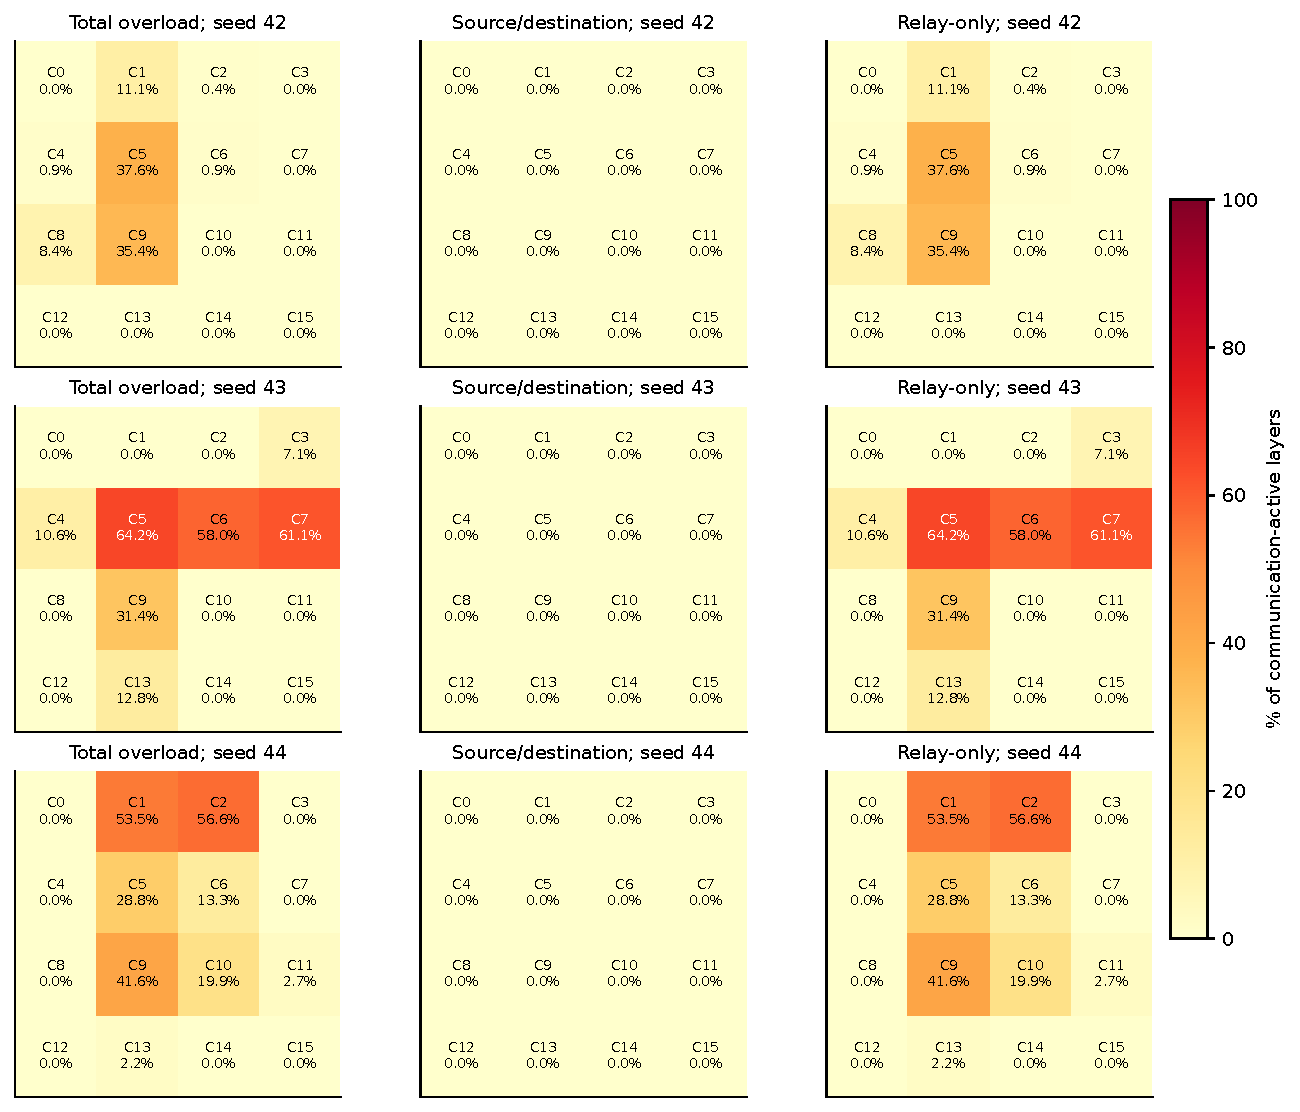
\includegraphics[width=.94\linewidth,height=.48\textheight,keepaspectratio]{figures/atlas/mesh_max_reliability_hop_m6.pdf}\captionof{figure}{All three conceptual mapping seeds; common 0--100 percent colour scale.}\end{center}
\begin{center}{\scriptsize\setlength{\tabcolsep}{3pt}
\begin{tabular}{lrrrrrrrrr}
\toprule
Core & 42 Tot & 42 Own & 42 Rel & 43 Tot & 43 Own & 43 Rel & 44 Tot & 44 Own & 44 Rel \\
\midrule
0 & 0.000 & 0.000 & 0.000 & 0.000 & 0.000 & 0.000 & 0.000 & 0.000 & 0.000 \\
1 & 11.062 & 0.000 & 11.062 & 0.000 & 0.000 & 0.000 & 53.540 & 0.000 & 53.540 \\
2 & 0.442 & 0.000 & 0.442 & 0.000 & 0.000 & 0.000 & 56.637 & 0.000 & 56.637 \\
3 & 0.000 & 0.000 & 0.000 & 7.080 & 0.000 & 7.080 & 0.000 & 0.000 & 0.000 \\
4 & 0.885 & 0.000 & 0.885 & 10.619 & 0.000 & 10.619 & 0.000 & 0.000 & 0.000 \\
5 & 37.611 & 0.000 & 37.611 & 64.159 & 0.000 & 64.159 & 28.761 & 0.000 & 28.761 \\
6 & 0.885 & 0.000 & 0.885 & 57.965 & 0.000 & 57.965 & 13.274 & 0.000 & 13.274 \\
7 & 0.000 & 0.000 & 0.000 & 61.062 & 0.000 & 61.062 & 0.000 & 0.000 & 0.000 \\
8 & 8.407 & 0.000 & 8.407 & 0.000 & 0.000 & 0.000 & 0.000 & 0.000 & 0.000 \\
9 & 35.398 & 0.000 & 35.398 & 31.416 & 0.000 & 31.416 & 41.593 & 0.000 & 41.593 \\
10 & 0.000 & 0.000 & 0.000 & 0.000 & 0.000 & 0.000 & 19.912 & 0.000 & 19.912 \\
11 & 0.000 & 0.000 & 0.000 & 0.000 & 0.000 & 0.000 & 2.655 & 0.000 & 2.655 \\
12 & 0.000 & 0.000 & 0.000 & 0.000 & 0.000 & 0.000 & 0.000 & 0.000 & 0.000 \\
13 & 0.000 & 0.000 & 0.000 & 12.832 & 0.000 & 12.832 & 2.212 & 0.000 & 2.212 \\
14 & 0.000 & 0.000 & 0.000 & 0.000 & 0.000 & 0.000 & 0.000 & 0.000 & 0.000 \\
15 & 0.000 & 0.000 & 0.000 & 0.000 & 0.000 & 0.000 & 0.000 & 0.000 & 0.000 \\
\bottomrule\end{tabular}}
\captionof{table}{Exact heatmap percentages, with Tot = Own + Rel. Unrounded values are in the CSV.}
{\footnotesize\href{https://github.com/sanjeevkrishnaa/Compiler-Driven-ACE/blob/codex/ace-scheduler-correctness/docs/latex/qft96_final/data/heatmap_mesh_max_reliability_hop_m6.csv}{Exact CSV values and sample counts}}
\end{center}
\clearpage\subsection*{Mesh max\_reliability; M=8; hop counting}
\begin{center}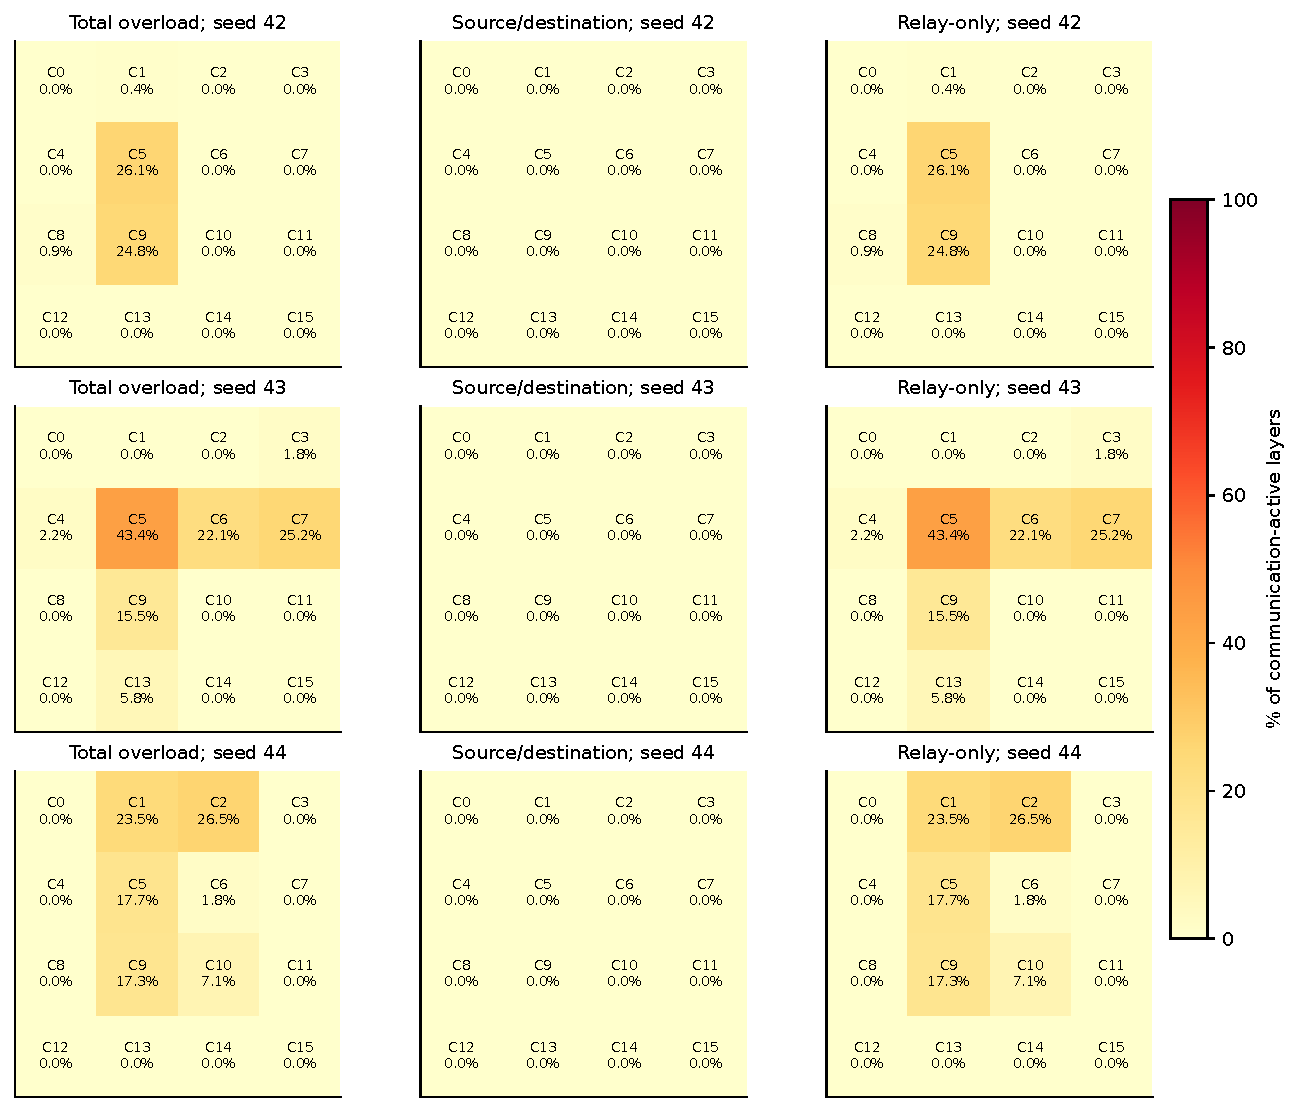
\includegraphics[width=.94\linewidth,height=.48\textheight,keepaspectratio]{figures/atlas/mesh_max_reliability_hop_m8.pdf}\captionof{figure}{All three conceptual mapping seeds; common 0--100 percent colour scale.}\end{center}
\begin{center}{\scriptsize\setlength{\tabcolsep}{3pt}
\begin{tabular}{lrrrrrrrrr}
\toprule
Core & 42 Tot & 42 Own & 42 Rel & 43 Tot & 43 Own & 43 Rel & 44 Tot & 44 Own & 44 Rel \\
\midrule
0 & 0.000 & 0.000 & 0.000 & 0.000 & 0.000 & 0.000 & 0.000 & 0.000 & 0.000 \\
1 & 0.442 & 0.000 & 0.442 & 0.000 & 0.000 & 0.000 & 23.451 & 0.000 & 23.451 \\
2 & 0.000 & 0.000 & 0.000 & 0.000 & 0.000 & 0.000 & 26.549 & 0.000 & 26.549 \\
3 & 0.000 & 0.000 & 0.000 & 1.770 & 0.000 & 1.770 & 0.000 & 0.000 & 0.000 \\
4 & 0.000 & 0.000 & 0.000 & 2.212 & 0.000 & 2.212 & 0.000 & 0.000 & 0.000 \\
5 & 26.106 & 0.000 & 26.106 & 43.363 & 0.000 & 43.363 & 17.699 & 0.000 & 17.699 \\
6 & 0.000 & 0.000 & 0.000 & 22.124 & 0.000 & 22.124 & 1.770 & 0.000 & 1.770 \\
7 & 0.000 & 0.000 & 0.000 & 25.221 & 0.000 & 25.221 & 0.000 & 0.000 & 0.000 \\
8 & 0.885 & 0.000 & 0.885 & 0.000 & 0.000 & 0.000 & 0.000 & 0.000 & 0.000 \\
9 & 24.779 & 0.000 & 24.779 & 15.487 & 0.000 & 15.487 & 17.257 & 0.000 & 17.257 \\
10 & 0.000 & 0.000 & 0.000 & 0.000 & 0.000 & 0.000 & 7.080 & 0.000 & 7.080 \\
11 & 0.000 & 0.000 & 0.000 & 0.000 & 0.000 & 0.000 & 0.000 & 0.000 & 0.000 \\
12 & 0.000 & 0.000 & 0.000 & 0.000 & 0.000 & 0.000 & 0.000 & 0.000 & 0.000 \\
13 & 0.000 & 0.000 & 0.000 & 5.752 & 0.000 & 5.752 & 0.000 & 0.000 & 0.000 \\
14 & 0.000 & 0.000 & 0.000 & 0.000 & 0.000 & 0.000 & 0.000 & 0.000 & 0.000 \\
15 & 0.000 & 0.000 & 0.000 & 0.000 & 0.000 & 0.000 & 0.000 & 0.000 & 0.000 \\
\bottomrule\end{tabular}}
\captionof{table}{Exact heatmap percentages, with Tot = Own + Rel. Unrounded values are in the CSV.}
{\footnotesize\href{https://github.com/sanjeevkrishnaa/Compiler-Driven-ACE/blob/codex/ace-scheduler-correctness/docs/latex/qft96_final/data/heatmap_mesh_max_reliability_hop_m8.csv}{Exact CSV values and sample counts}}
\end{center}
\clearpage\subsection*{Mesh max\_reliability; M=16; hop counting}
\begin{center}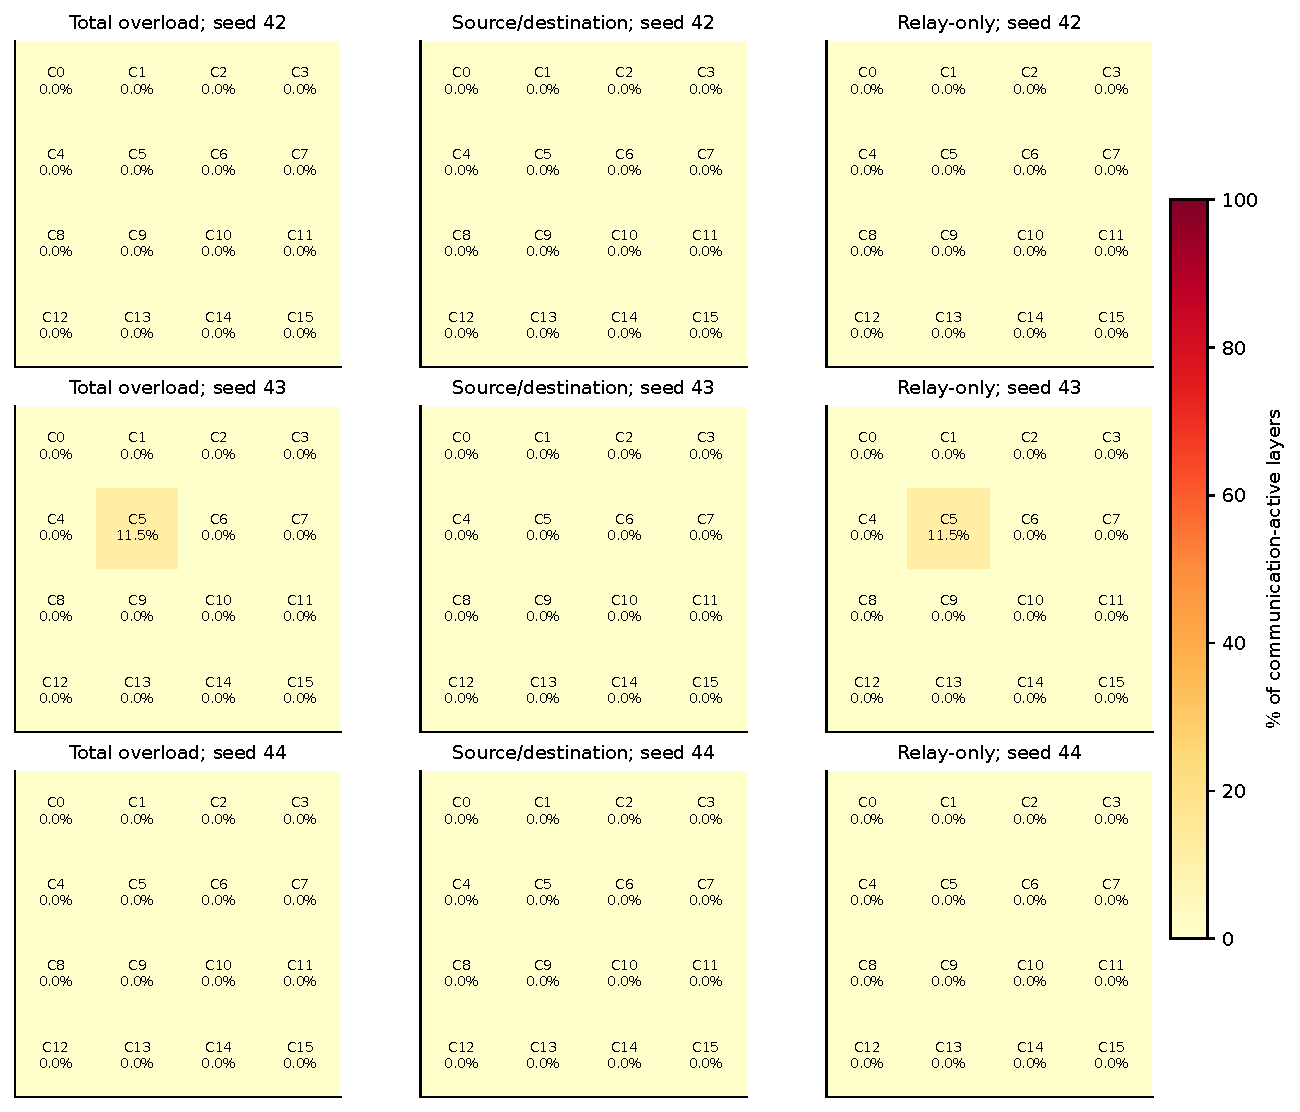
\includegraphics[width=.94\linewidth,height=.48\textheight,keepaspectratio]{figures/atlas/mesh_max_reliability_hop_m16.pdf}\captionof{figure}{All three conceptual mapping seeds; common 0--100 percent colour scale.}\end{center}
\begin{center}{\scriptsize\setlength{\tabcolsep}{3pt}
\begin{tabular}{lrrrrrrrrr}
\toprule
Core & 42 Tot & 42 Own & 42 Rel & 43 Tot & 43 Own & 43 Rel & 44 Tot & 44 Own & 44 Rel \\
\midrule
0 & 0.000 & 0.000 & 0.000 & 0.000 & 0.000 & 0.000 & 0.000 & 0.000 & 0.000 \\
1 & 0.000 & 0.000 & 0.000 & 0.000 & 0.000 & 0.000 & 0.000 & 0.000 & 0.000 \\
2 & 0.000 & 0.000 & 0.000 & 0.000 & 0.000 & 0.000 & 0.000 & 0.000 & 0.000 \\
3 & 0.000 & 0.000 & 0.000 & 0.000 & 0.000 & 0.000 & 0.000 & 0.000 & 0.000 \\
4 & 0.000 & 0.000 & 0.000 & 0.000 & 0.000 & 0.000 & 0.000 & 0.000 & 0.000 \\
5 & 0.000 & 0.000 & 0.000 & 11.504 & 0.000 & 11.504 & 0.000 & 0.000 & 0.000 \\
6 & 0.000 & 0.000 & 0.000 & 0.000 & 0.000 & 0.000 & 0.000 & 0.000 & 0.000 \\
7 & 0.000 & 0.000 & 0.000 & 0.000 & 0.000 & 0.000 & 0.000 & 0.000 & 0.000 \\
8 & 0.000 & 0.000 & 0.000 & 0.000 & 0.000 & 0.000 & 0.000 & 0.000 & 0.000 \\
9 & 0.000 & 0.000 & 0.000 & 0.000 & 0.000 & 0.000 & 0.000 & 0.000 & 0.000 \\
10 & 0.000 & 0.000 & 0.000 & 0.000 & 0.000 & 0.000 & 0.000 & 0.000 & 0.000 \\
11 & 0.000 & 0.000 & 0.000 & 0.000 & 0.000 & 0.000 & 0.000 & 0.000 & 0.000 \\
12 & 0.000 & 0.000 & 0.000 & 0.000 & 0.000 & 0.000 & 0.000 & 0.000 & 0.000 \\
13 & 0.000 & 0.000 & 0.000 & 0.000 & 0.000 & 0.000 & 0.000 & 0.000 & 0.000 \\
14 & 0.000 & 0.000 & 0.000 & 0.000 & 0.000 & 0.000 & 0.000 & 0.000 & 0.000 \\
15 & 0.000 & 0.000 & 0.000 & 0.000 & 0.000 & 0.000 & 0.000 & 0.000 & 0.000 \\
\bottomrule\end{tabular}}
\captionof{table}{Exact heatmap percentages, with Tot = Own + Rel. Unrounded values are in the CSV.}
{\footnotesize\href{https://github.com/sanjeevkrishnaa/Compiler-Driven-ACE/blob/codex/ace-scheduler-correctness/docs/latex/qft96_final/data/heatmap_mesh_max_reliability_hop_m16.csv}{Exact CSV values and sample counts}}
\end{center}
\clearpage\subsection*{Mesh max\_reliability; M=32; hop counting}
\begin{center}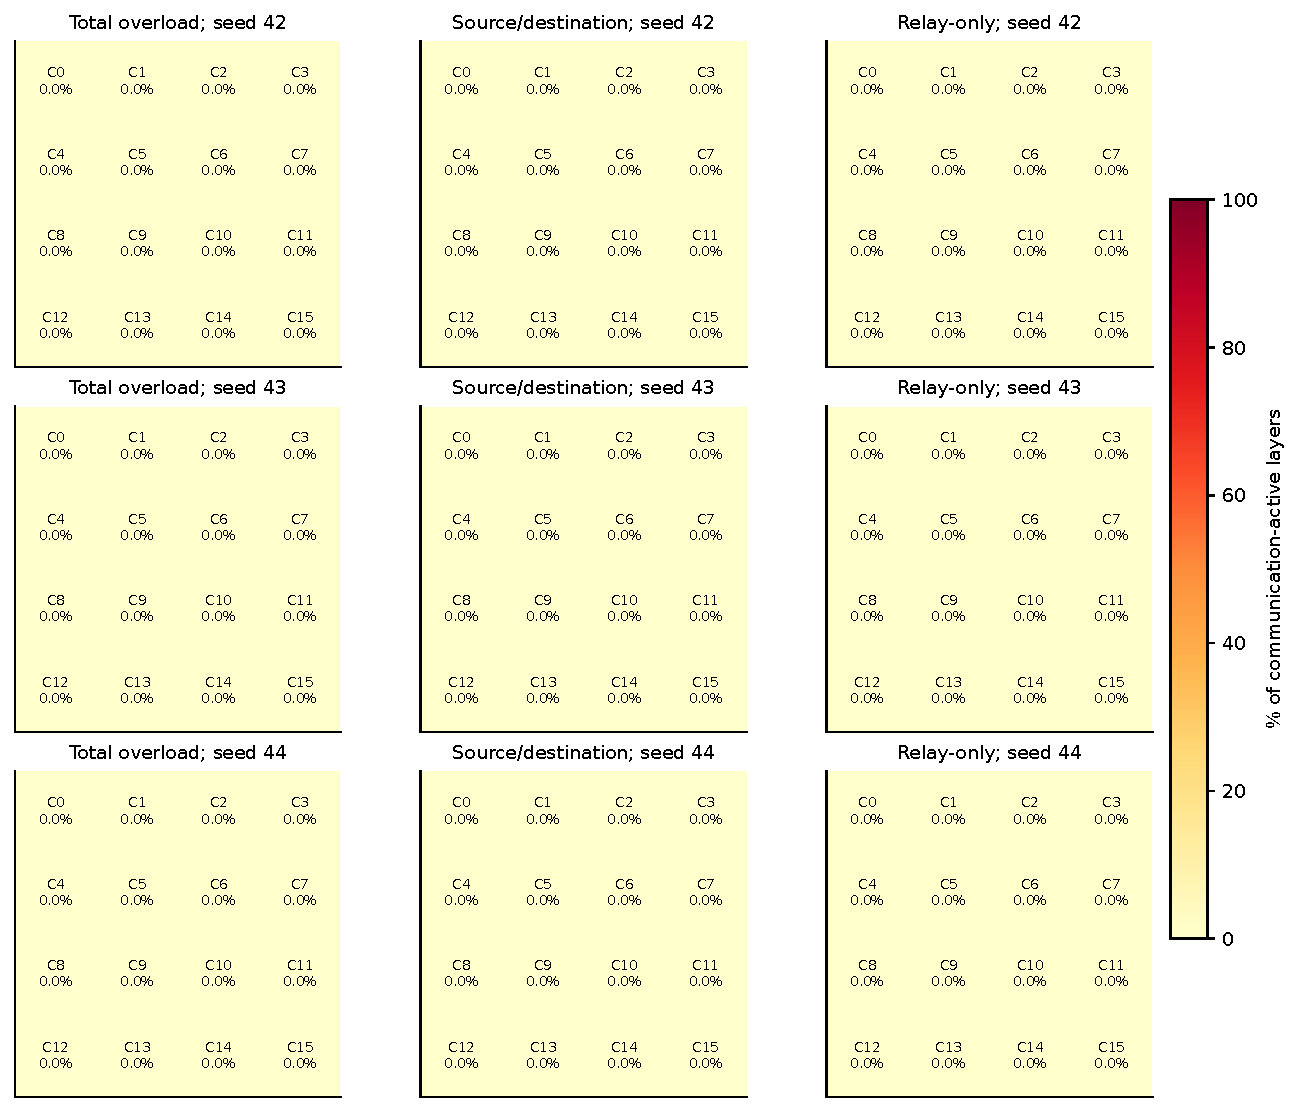
\includegraphics[width=.94\linewidth,height=.48\textheight,keepaspectratio]{figures/atlas/mesh_max_reliability_hop_m32.pdf}\captionof{figure}{All three conceptual mapping seeds; common 0--100 percent colour scale.}\end{center}
\begin{center}{\scriptsize\setlength{\tabcolsep}{3pt}
\begin{tabular}{lrrrrrrrrr}
\toprule
Core & 42 Tot & 42 Own & 42 Rel & 43 Tot & 43 Own & 43 Rel & 44 Tot & 44 Own & 44 Rel \\
\midrule
0 & 0.000 & 0.000 & 0.000 & 0.000 & 0.000 & 0.000 & 0.000 & 0.000 & 0.000 \\
1 & 0.000 & 0.000 & 0.000 & 0.000 & 0.000 & 0.000 & 0.000 & 0.000 & 0.000 \\
2 & 0.000 & 0.000 & 0.000 & 0.000 & 0.000 & 0.000 & 0.000 & 0.000 & 0.000 \\
3 & 0.000 & 0.000 & 0.000 & 0.000 & 0.000 & 0.000 & 0.000 & 0.000 & 0.000 \\
4 & 0.000 & 0.000 & 0.000 & 0.000 & 0.000 & 0.000 & 0.000 & 0.000 & 0.000 \\
5 & 0.000 & 0.000 & 0.000 & 0.000 & 0.000 & 0.000 & 0.000 & 0.000 & 0.000 \\
6 & 0.000 & 0.000 & 0.000 & 0.000 & 0.000 & 0.000 & 0.000 & 0.000 & 0.000 \\
7 & 0.000 & 0.000 & 0.000 & 0.000 & 0.000 & 0.000 & 0.000 & 0.000 & 0.000 \\
8 & 0.000 & 0.000 & 0.000 & 0.000 & 0.000 & 0.000 & 0.000 & 0.000 & 0.000 \\
9 & 0.000 & 0.000 & 0.000 & 0.000 & 0.000 & 0.000 & 0.000 & 0.000 & 0.000 \\
10 & 0.000 & 0.000 & 0.000 & 0.000 & 0.000 & 0.000 & 0.000 & 0.000 & 0.000 \\
11 & 0.000 & 0.000 & 0.000 & 0.000 & 0.000 & 0.000 & 0.000 & 0.000 & 0.000 \\
12 & 0.000 & 0.000 & 0.000 & 0.000 & 0.000 & 0.000 & 0.000 & 0.000 & 0.000 \\
13 & 0.000 & 0.000 & 0.000 & 0.000 & 0.000 & 0.000 & 0.000 & 0.000 & 0.000 \\
14 & 0.000 & 0.000 & 0.000 & 0.000 & 0.000 & 0.000 & 0.000 & 0.000 & 0.000 \\
15 & 0.000 & 0.000 & 0.000 & 0.000 & 0.000 & 0.000 & 0.000 & 0.000 & 0.000 \\
\bottomrule\end{tabular}}
\captionof{table}{Exact heatmap percentages, with Tot = Own + Rel. Unrounded values are in the CSV.}
{\footnotesize\href{https://github.com/sanjeevkrishnaa/Compiler-Driven-ACE/blob/codex/ace-scheduler-correctness/docs/latex/qft96_final/data/heatmap_mesh_max_reliability_hop_m32.csv}{Exact CSV values and sample counts}}
\end{center}
\section{Torus / dijkstra}
\clearpage\subsection*{Torus dijkstra; M=2; route counting}
\begin{center}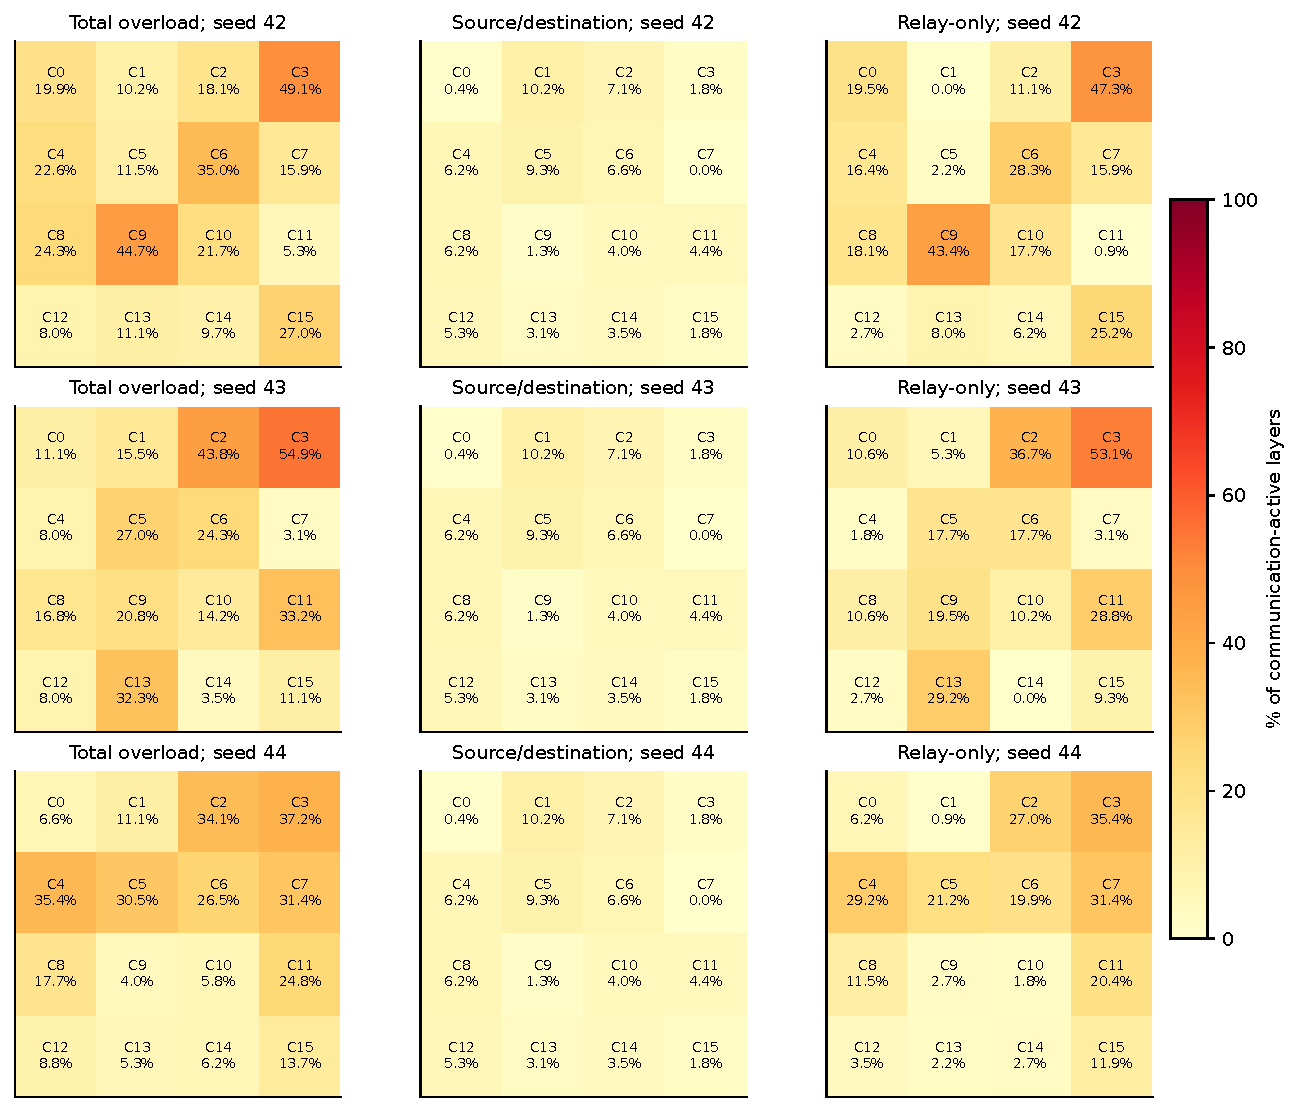
\includegraphics[width=.94\linewidth,height=.48\textheight,keepaspectratio]{figures/atlas/torus_dijkstra_route_m2.pdf}\captionof{figure}{All three conceptual mapping seeds; common 0--100 percent colour scale.}\end{center}
\begin{center}{\scriptsize\setlength{\tabcolsep}{3pt}
\begin{tabular}{lrrrrrrrrr}
\toprule
Core & 42 Tot & 42 Own & 42 Rel & 43 Tot & 43 Own & 43 Rel & 44 Tot & 44 Own & 44 Rel \\
\midrule
0 & 19.912 & 0.442 & 19.469 & 11.062 & 0.442 & 10.619 & 6.637 & 0.442 & 6.195 \\
1 & 10.177 & 10.177 & 0.000 & 15.487 & 10.177 & 5.310 & 11.062 & 10.177 & 0.885 \\
2 & 18.142 & 7.080 & 11.062 & 43.805 & 7.080 & 36.726 & 34.071 & 7.080 & 26.991 \\
3 & 49.115 & 1.770 & 47.345 & 54.867 & 1.770 & 53.097 & 37.168 & 1.770 & 35.398 \\
4 & 22.566 & 6.195 & 16.372 & 7.965 & 6.195 & 1.770 & 35.398 & 6.195 & 29.204 \\
5 & 11.504 & 9.292 & 2.212 & 26.991 & 9.292 & 17.699 & 30.531 & 9.292 & 21.239 \\
6 & 34.956 & 6.637 & 28.319 & 24.336 & 6.637 & 17.699 & 26.549 & 6.637 & 19.912 \\
7 & 15.929 & 0.000 & 15.929 & 3.097 & 0.000 & 3.097 & 31.416 & 0.000 & 31.416 \\
8 & 24.336 & 6.195 & 18.142 & 16.814 & 6.195 & 10.619 & 17.699 & 6.195 & 11.504 \\
9 & 44.690 & 1.327 & 43.363 & 20.796 & 1.327 & 19.469 & 3.982 & 1.327 & 2.655 \\
10 & 21.681 & 3.982 & 17.699 & 14.159 & 3.982 & 10.177 & 5.752 & 3.982 & 1.770 \\
11 & 5.310 & 4.425 & 0.885 & 33.186 & 4.425 & 28.761 & 24.779 & 4.425 & 20.354 \\
12 & 7.965 & 5.310 & 2.655 & 7.965 & 5.310 & 2.655 & 8.850 & 5.310 & 3.540 \\
13 & 11.062 & 3.097 & 7.965 & 32.301 & 3.097 & 29.204 & 5.310 & 3.097 & 2.212 \\
14 & 9.735 & 3.540 & 6.195 & 3.540 & 3.540 & 0.000 & 6.195 & 3.540 & 2.655 \\
15 & 26.991 & 1.770 & 25.221 & 11.062 & 1.770 & 9.292 & 13.717 & 1.770 & 11.947 \\
\bottomrule\end{tabular}}
\captionof{table}{Exact heatmap percentages, with Tot = Own + Rel. Unrounded values are in the CSV.}
{\footnotesize\href{https://github.com/sanjeevkrishnaa/Compiler-Driven-ACE/blob/codex/ace-scheduler-correctness/docs/latex/qft96_final/data/heatmap_torus_dijkstra_route_m2.csv}{Exact CSV values and sample counts}}
\end{center}
\clearpage\subsection*{Torus dijkstra; M=3; route counting}
\begin{center}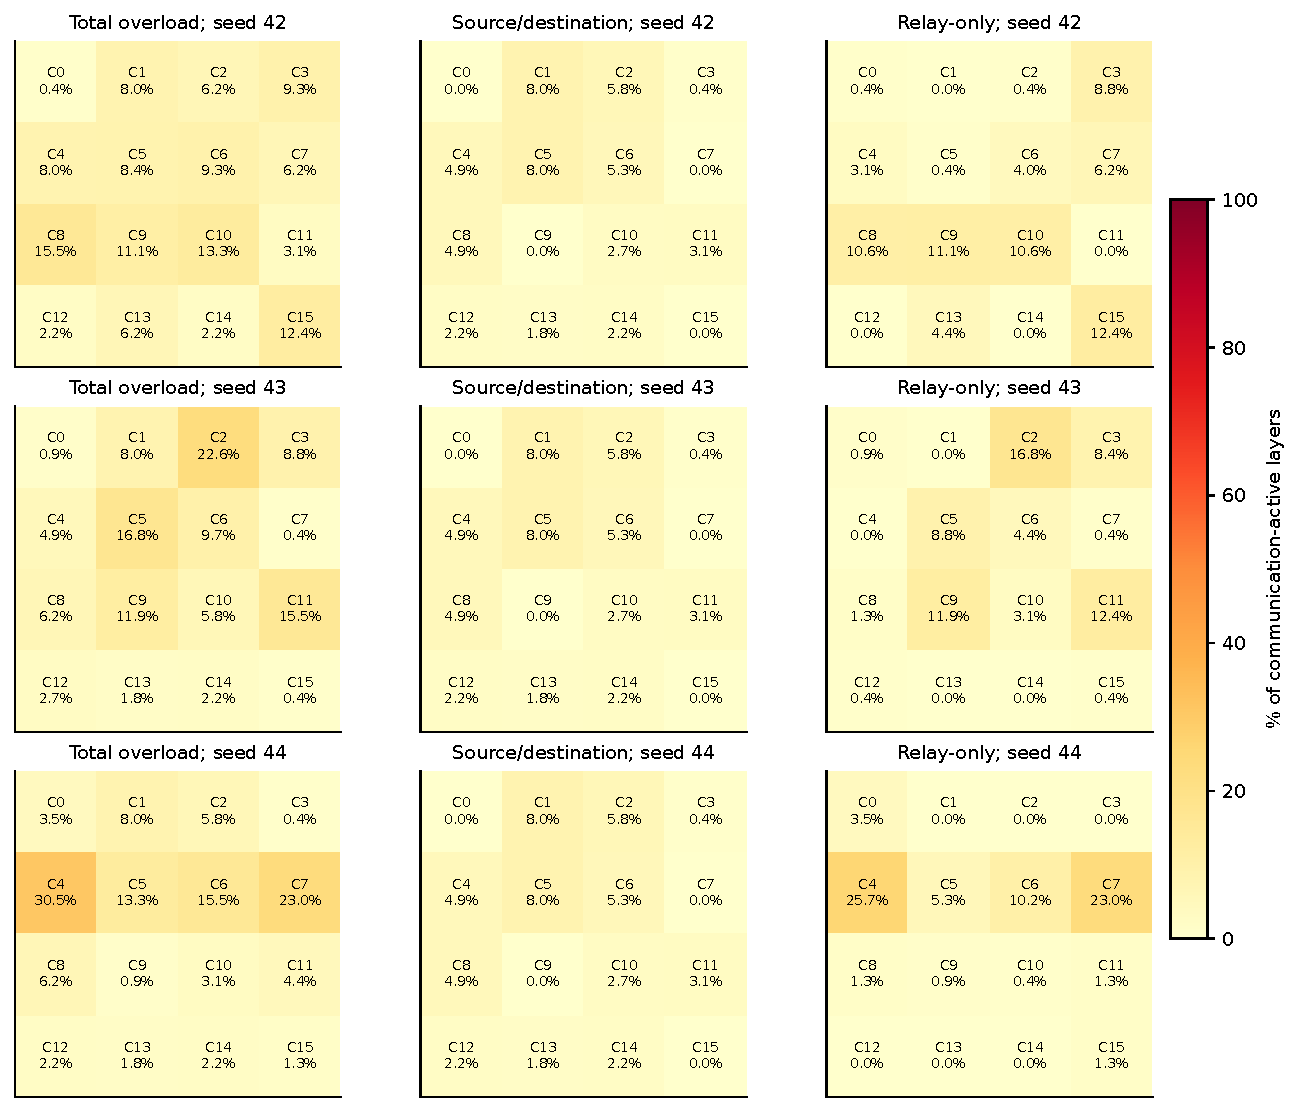
\includegraphics[width=.94\linewidth,height=.48\textheight,keepaspectratio]{figures/atlas/torus_dijkstra_route_m3.pdf}\captionof{figure}{All three conceptual mapping seeds; common 0--100 percent colour scale.}\end{center}
\begin{center}{\scriptsize\setlength{\tabcolsep}{3pt}
\begin{tabular}{lrrrrrrrrr}
\toprule
Core & 42 Tot & 42 Own & 42 Rel & 43 Tot & 43 Own & 43 Rel & 44 Tot & 44 Own & 44 Rel \\
\midrule
0 & 0.442 & 0.000 & 0.442 & 0.885 & 0.000 & 0.885 & 3.540 & 0.000 & 3.540 \\
1 & 7.965 & 7.965 & 0.000 & 7.965 & 7.965 & 0.000 & 7.965 & 7.965 & 0.000 \\
2 & 6.195 & 5.752 & 0.442 & 22.566 & 5.752 & 16.814 & 5.752 & 5.752 & 0.000 \\
3 & 9.292 & 0.442 & 8.850 & 8.850 & 0.442 & 8.407 & 0.442 & 0.442 & 0.000 \\
4 & 7.965 & 4.867 & 3.097 & 4.867 & 4.867 & 0.000 & 30.531 & 4.867 & 25.664 \\
5 & 8.407 & 7.965 & 0.442 & 16.814 & 7.965 & 8.850 & 13.274 & 7.965 & 5.310 \\
6 & 9.292 & 5.310 & 3.982 & 9.735 & 5.310 & 4.425 & 15.487 & 5.310 & 10.177 \\
7 & 6.195 & 0.000 & 6.195 & 0.442 & 0.000 & 0.442 & 23.009 & 0.000 & 23.009 \\
8 & 15.487 & 4.867 & 10.619 & 6.195 & 4.867 & 1.327 & 6.195 & 4.867 & 1.327 \\
9 & 11.062 & 0.000 & 11.062 & 11.947 & 0.000 & 11.947 & 0.885 & 0.000 & 0.885 \\
10 & 13.274 & 2.655 & 10.619 & 5.752 & 2.655 & 3.097 & 3.097 & 2.655 & 0.442 \\
11 & 3.097 & 3.097 & 0.000 & 15.487 & 3.097 & 12.389 & 4.425 & 3.097 & 1.327 \\
12 & 2.212 & 2.212 & 0.000 & 2.655 & 2.212 & 0.442 & 2.212 & 2.212 & 0.000 \\
13 & 6.195 & 1.770 & 4.425 & 1.770 & 1.770 & 0.000 & 1.770 & 1.770 & 0.000 \\
14 & 2.212 & 2.212 & 0.000 & 2.212 & 2.212 & 0.000 & 2.212 & 2.212 & 0.000 \\
15 & 12.389 & 0.000 & 12.389 & 0.442 & 0.000 & 0.442 & 1.327 & 0.000 & 1.327 \\
\bottomrule\end{tabular}}
\captionof{table}{Exact heatmap percentages, with Tot = Own + Rel. Unrounded values are in the CSV.}
{\footnotesize\href{https://github.com/sanjeevkrishnaa/Compiler-Driven-ACE/blob/codex/ace-scheduler-correctness/docs/latex/qft96_final/data/heatmap_torus_dijkstra_route_m3.csv}{Exact CSV values and sample counts}}
\end{center}
\clearpage\subsection*{Torus dijkstra; M=4; route counting}
\begin{center}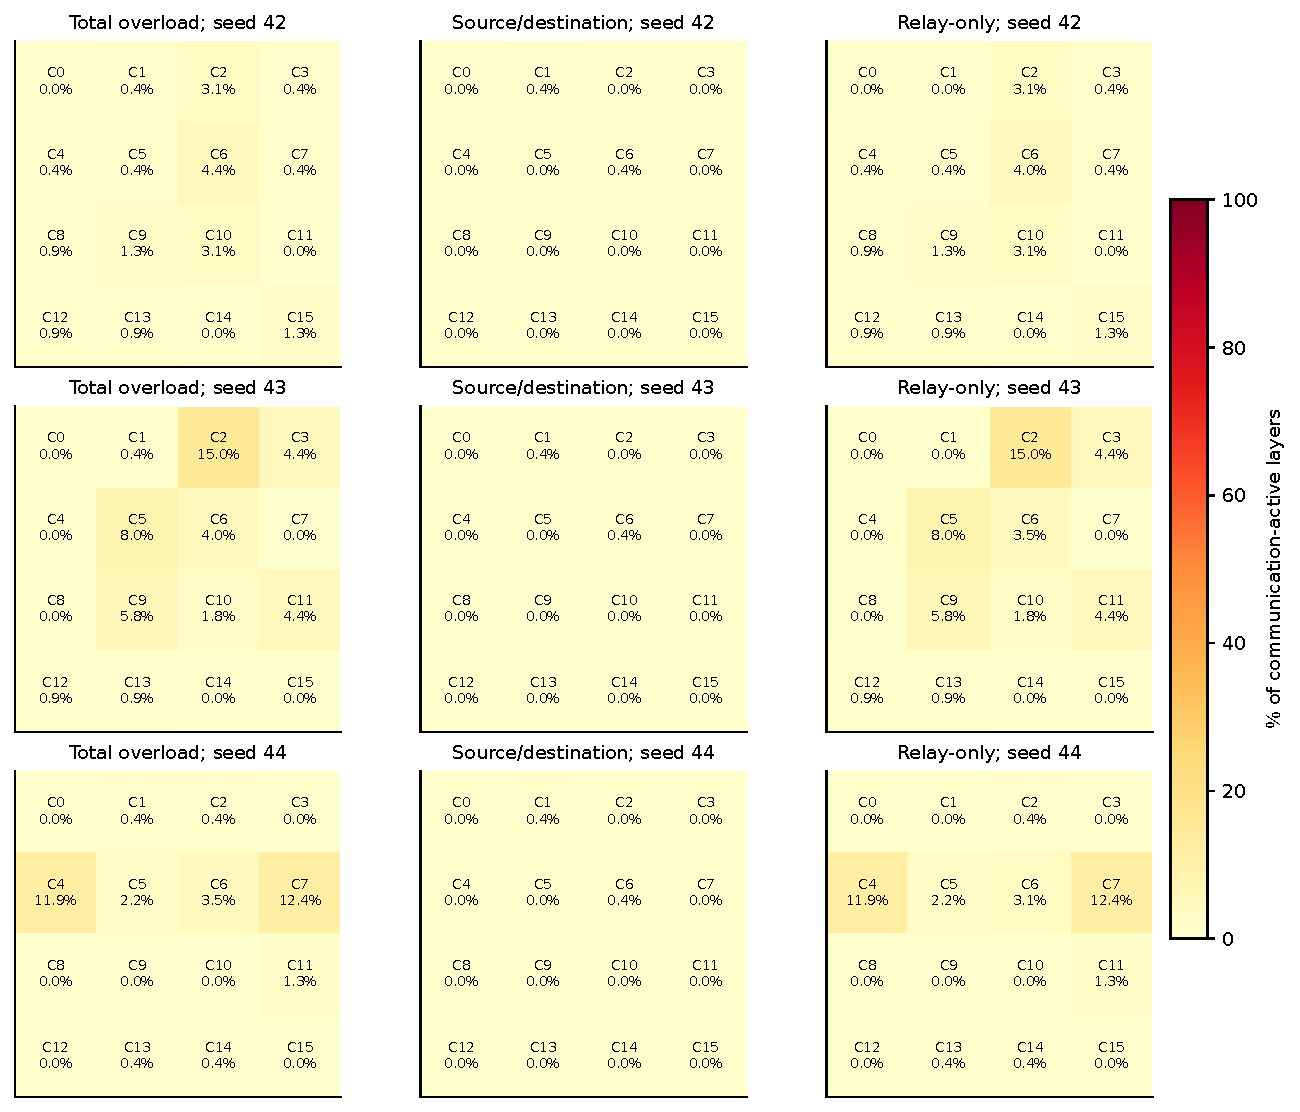
\includegraphics[width=.94\linewidth,height=.48\textheight,keepaspectratio]{figures/atlas/torus_dijkstra_route_m4.pdf}\captionof{figure}{All three conceptual mapping seeds; common 0--100 percent colour scale.}\end{center}
\begin{center}{\scriptsize\setlength{\tabcolsep}{3pt}
\begin{tabular}{lrrrrrrrrr}
\toprule
Core & 42 Tot & 42 Own & 42 Rel & 43 Tot & 43 Own & 43 Rel & 44 Tot & 44 Own & 44 Rel \\
\midrule
0 & 0.000 & 0.000 & 0.000 & 0.000 & 0.000 & 0.000 & 0.000 & 0.000 & 0.000 \\
1 & 0.442 & 0.442 & 0.000 & 0.442 & 0.442 & 0.000 & 0.442 & 0.442 & 0.000 \\
2 & 3.097 & 0.000 & 3.097 & 15.044 & 0.000 & 15.044 & 0.442 & 0.000 & 0.442 \\
3 & 0.442 & 0.000 & 0.442 & 4.425 & 0.000 & 4.425 & 0.000 & 0.000 & 0.000 \\
4 & 0.442 & 0.000 & 0.442 & 0.000 & 0.000 & 0.000 & 11.947 & 0.000 & 11.947 \\
5 & 0.442 & 0.000 & 0.442 & 7.965 & 0.000 & 7.965 & 2.212 & 0.000 & 2.212 \\
6 & 4.425 & 0.442 & 3.982 & 3.982 & 0.442 & 3.540 & 3.540 & 0.442 & 3.097 \\
7 & 0.442 & 0.000 & 0.442 & 0.000 & 0.000 & 0.000 & 12.389 & 0.000 & 12.389 \\
8 & 0.885 & 0.000 & 0.885 & 0.000 & 0.000 & 0.000 & 0.000 & 0.000 & 0.000 \\
9 & 1.327 & 0.000 & 1.327 & 5.752 & 0.000 & 5.752 & 0.000 & 0.000 & 0.000 \\
10 & 3.097 & 0.000 & 3.097 & 1.770 & 0.000 & 1.770 & 0.000 & 0.000 & 0.000 \\
11 & 0.000 & 0.000 & 0.000 & 4.425 & 0.000 & 4.425 & 1.327 & 0.000 & 1.327 \\
12 & 0.885 & 0.000 & 0.885 & 0.885 & 0.000 & 0.885 & 0.000 & 0.000 & 0.000 \\
13 & 0.885 & 0.000 & 0.885 & 0.885 & 0.000 & 0.885 & 0.442 & 0.000 & 0.442 \\
14 & 0.000 & 0.000 & 0.000 & 0.000 & 0.000 & 0.000 & 0.442 & 0.000 & 0.442 \\
15 & 1.327 & 0.000 & 1.327 & 0.000 & 0.000 & 0.000 & 0.000 & 0.000 & 0.000 \\
\bottomrule\end{tabular}}
\captionof{table}{Exact heatmap percentages, with Tot = Own + Rel. Unrounded values are in the CSV.}
{\footnotesize\href{https://github.com/sanjeevkrishnaa/Compiler-Driven-ACE/blob/codex/ace-scheduler-correctness/docs/latex/qft96_final/data/heatmap_torus_dijkstra_route_m4.csv}{Exact CSV values and sample counts}}
\end{center}
\clearpage\subsection*{Torus dijkstra; M=6; route counting}
\begin{center}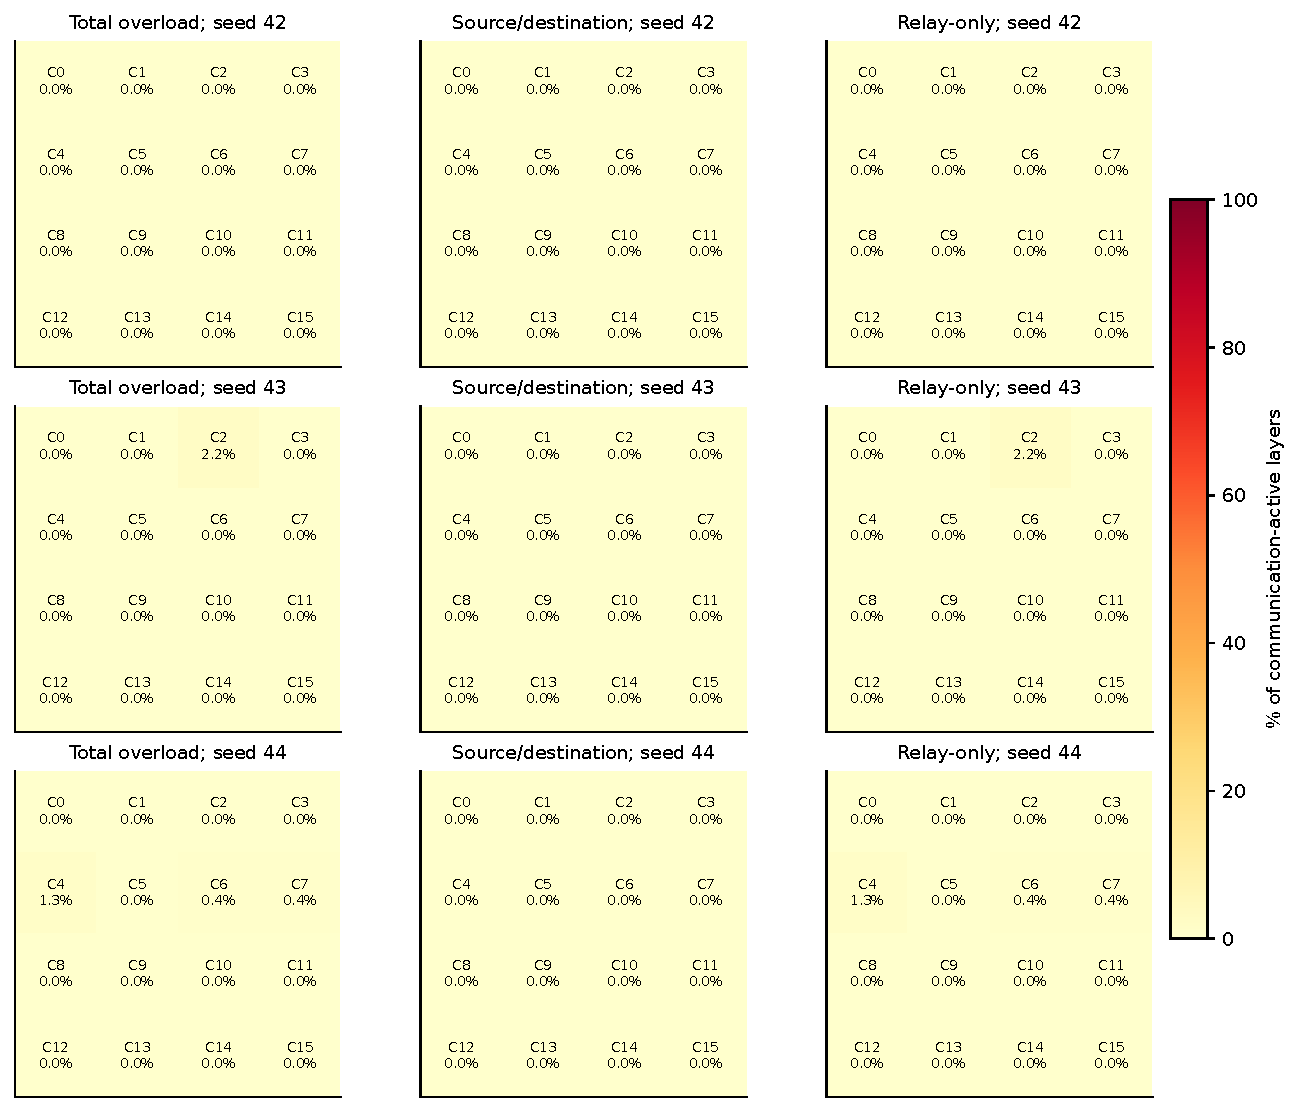
\includegraphics[width=.94\linewidth,height=.48\textheight,keepaspectratio]{figures/atlas/torus_dijkstra_route_m6.pdf}\captionof{figure}{All three conceptual mapping seeds; common 0--100 percent colour scale.}\end{center}
\begin{center}{\scriptsize\setlength{\tabcolsep}{3pt}
\begin{tabular}{lrrrrrrrrr}
\toprule
Core & 42 Tot & 42 Own & 42 Rel & 43 Tot & 43 Own & 43 Rel & 44 Tot & 44 Own & 44 Rel \\
\midrule
0 & 0.000 & 0.000 & 0.000 & 0.000 & 0.000 & 0.000 & 0.000 & 0.000 & 0.000 \\
1 & 0.000 & 0.000 & 0.000 & 0.000 & 0.000 & 0.000 & 0.000 & 0.000 & 0.000 \\
2 & 0.000 & 0.000 & 0.000 & 2.212 & 0.000 & 2.212 & 0.000 & 0.000 & 0.000 \\
3 & 0.000 & 0.000 & 0.000 & 0.000 & 0.000 & 0.000 & 0.000 & 0.000 & 0.000 \\
4 & 0.000 & 0.000 & 0.000 & 0.000 & 0.000 & 0.000 & 1.327 & 0.000 & 1.327 \\
5 & 0.000 & 0.000 & 0.000 & 0.000 & 0.000 & 0.000 & 0.000 & 0.000 & 0.000 \\
6 & 0.000 & 0.000 & 0.000 & 0.000 & 0.000 & 0.000 & 0.442 & 0.000 & 0.442 \\
7 & 0.000 & 0.000 & 0.000 & 0.000 & 0.000 & 0.000 & 0.442 & 0.000 & 0.442 \\
8 & 0.000 & 0.000 & 0.000 & 0.000 & 0.000 & 0.000 & 0.000 & 0.000 & 0.000 \\
9 & 0.000 & 0.000 & 0.000 & 0.000 & 0.000 & 0.000 & 0.000 & 0.000 & 0.000 \\
10 & 0.000 & 0.000 & 0.000 & 0.000 & 0.000 & 0.000 & 0.000 & 0.000 & 0.000 \\
11 & 0.000 & 0.000 & 0.000 & 0.000 & 0.000 & 0.000 & 0.000 & 0.000 & 0.000 \\
12 & 0.000 & 0.000 & 0.000 & 0.000 & 0.000 & 0.000 & 0.000 & 0.000 & 0.000 \\
13 & 0.000 & 0.000 & 0.000 & 0.000 & 0.000 & 0.000 & 0.000 & 0.000 & 0.000 \\
14 & 0.000 & 0.000 & 0.000 & 0.000 & 0.000 & 0.000 & 0.000 & 0.000 & 0.000 \\
15 & 0.000 & 0.000 & 0.000 & 0.000 & 0.000 & 0.000 & 0.000 & 0.000 & 0.000 \\
\bottomrule\end{tabular}}
\captionof{table}{Exact heatmap percentages, with Tot = Own + Rel. Unrounded values are in the CSV.}
{\footnotesize\href{https://github.com/sanjeevkrishnaa/Compiler-Driven-ACE/blob/codex/ace-scheduler-correctness/docs/latex/qft96_final/data/heatmap_torus_dijkstra_route_m6.csv}{Exact CSV values and sample counts}}
\end{center}
\clearpage\subsection*{Torus dijkstra; M=8; route counting}
\begin{center}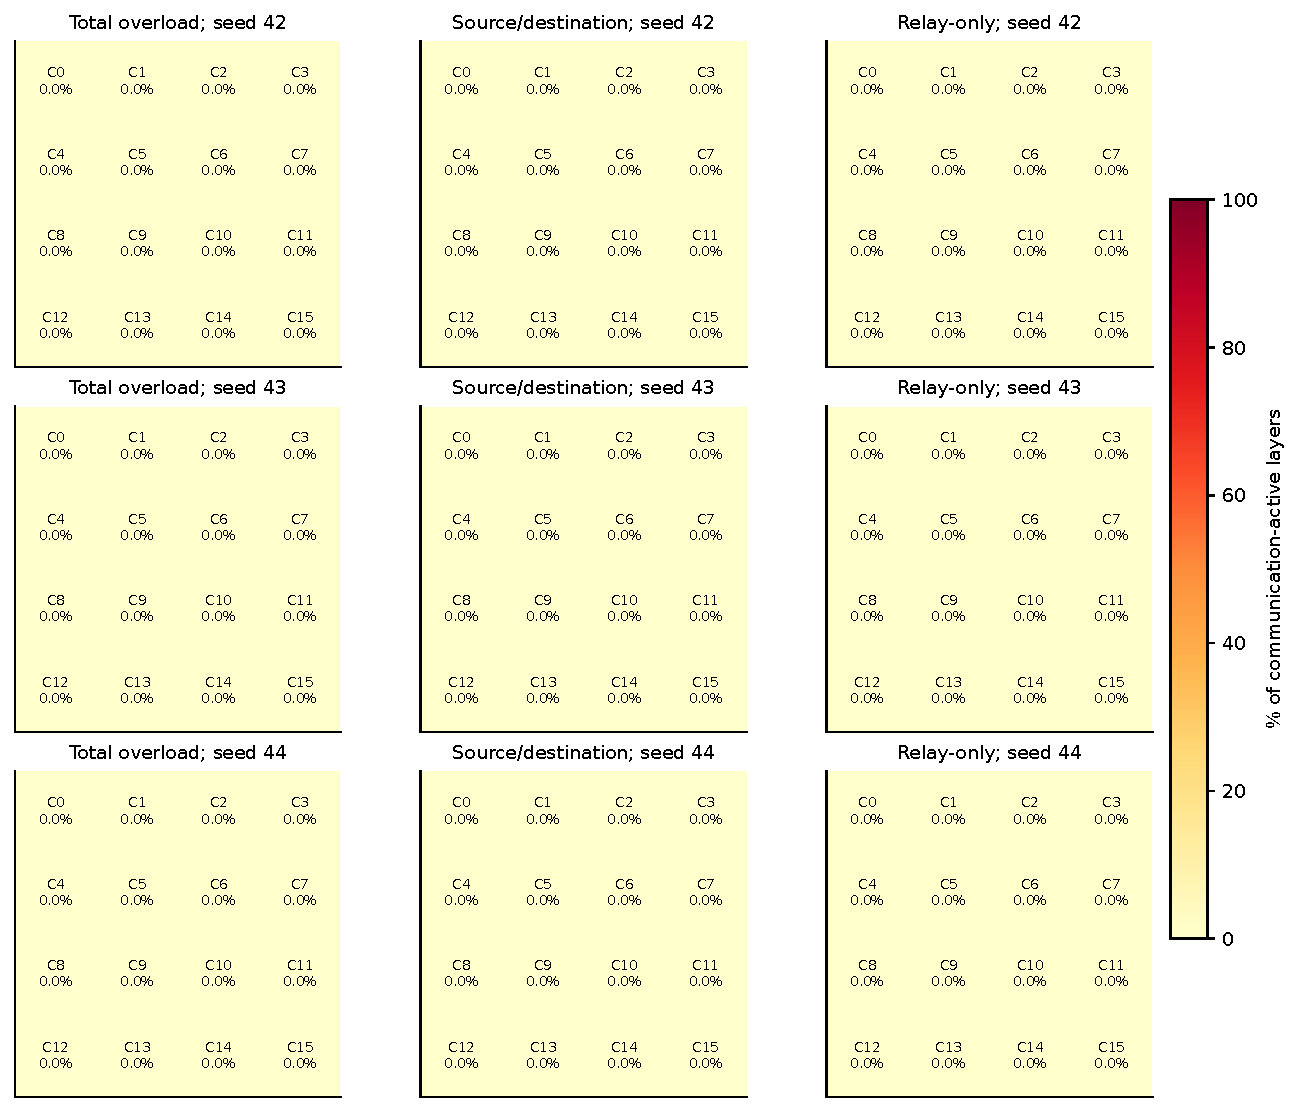
\includegraphics[width=.94\linewidth,height=.48\textheight,keepaspectratio]{figures/atlas/torus_dijkstra_route_m8.pdf}\captionof{figure}{All three conceptual mapping seeds; common 0--100 percent colour scale.}\end{center}
\begin{center}{\scriptsize\setlength{\tabcolsep}{3pt}
\begin{tabular}{lrrrrrrrrr}
\toprule
Core & 42 Tot & 42 Own & 42 Rel & 43 Tot & 43 Own & 43 Rel & 44 Tot & 44 Own & 44 Rel \\
\midrule
0 & 0.000 & 0.000 & 0.000 & 0.000 & 0.000 & 0.000 & 0.000 & 0.000 & 0.000 \\
1 & 0.000 & 0.000 & 0.000 & 0.000 & 0.000 & 0.000 & 0.000 & 0.000 & 0.000 \\
2 & 0.000 & 0.000 & 0.000 & 0.000 & 0.000 & 0.000 & 0.000 & 0.000 & 0.000 \\
3 & 0.000 & 0.000 & 0.000 & 0.000 & 0.000 & 0.000 & 0.000 & 0.000 & 0.000 \\
4 & 0.000 & 0.000 & 0.000 & 0.000 & 0.000 & 0.000 & 0.000 & 0.000 & 0.000 \\
5 & 0.000 & 0.000 & 0.000 & 0.000 & 0.000 & 0.000 & 0.000 & 0.000 & 0.000 \\
6 & 0.000 & 0.000 & 0.000 & 0.000 & 0.000 & 0.000 & 0.000 & 0.000 & 0.000 \\
7 & 0.000 & 0.000 & 0.000 & 0.000 & 0.000 & 0.000 & 0.000 & 0.000 & 0.000 \\
8 & 0.000 & 0.000 & 0.000 & 0.000 & 0.000 & 0.000 & 0.000 & 0.000 & 0.000 \\
9 & 0.000 & 0.000 & 0.000 & 0.000 & 0.000 & 0.000 & 0.000 & 0.000 & 0.000 \\
10 & 0.000 & 0.000 & 0.000 & 0.000 & 0.000 & 0.000 & 0.000 & 0.000 & 0.000 \\
11 & 0.000 & 0.000 & 0.000 & 0.000 & 0.000 & 0.000 & 0.000 & 0.000 & 0.000 \\
12 & 0.000 & 0.000 & 0.000 & 0.000 & 0.000 & 0.000 & 0.000 & 0.000 & 0.000 \\
13 & 0.000 & 0.000 & 0.000 & 0.000 & 0.000 & 0.000 & 0.000 & 0.000 & 0.000 \\
14 & 0.000 & 0.000 & 0.000 & 0.000 & 0.000 & 0.000 & 0.000 & 0.000 & 0.000 \\
15 & 0.000 & 0.000 & 0.000 & 0.000 & 0.000 & 0.000 & 0.000 & 0.000 & 0.000 \\
\bottomrule\end{tabular}}
\captionof{table}{Exact heatmap percentages, with Tot = Own + Rel. Unrounded values are in the CSV.}
{\footnotesize\href{https://github.com/sanjeevkrishnaa/Compiler-Driven-ACE/blob/codex/ace-scheduler-correctness/docs/latex/qft96_final/data/heatmap_torus_dijkstra_route_m8.csv}{Exact CSV values and sample counts}}
\end{center}
\clearpage\subsection*{Torus dijkstra; M=16; route counting}
\begin{center}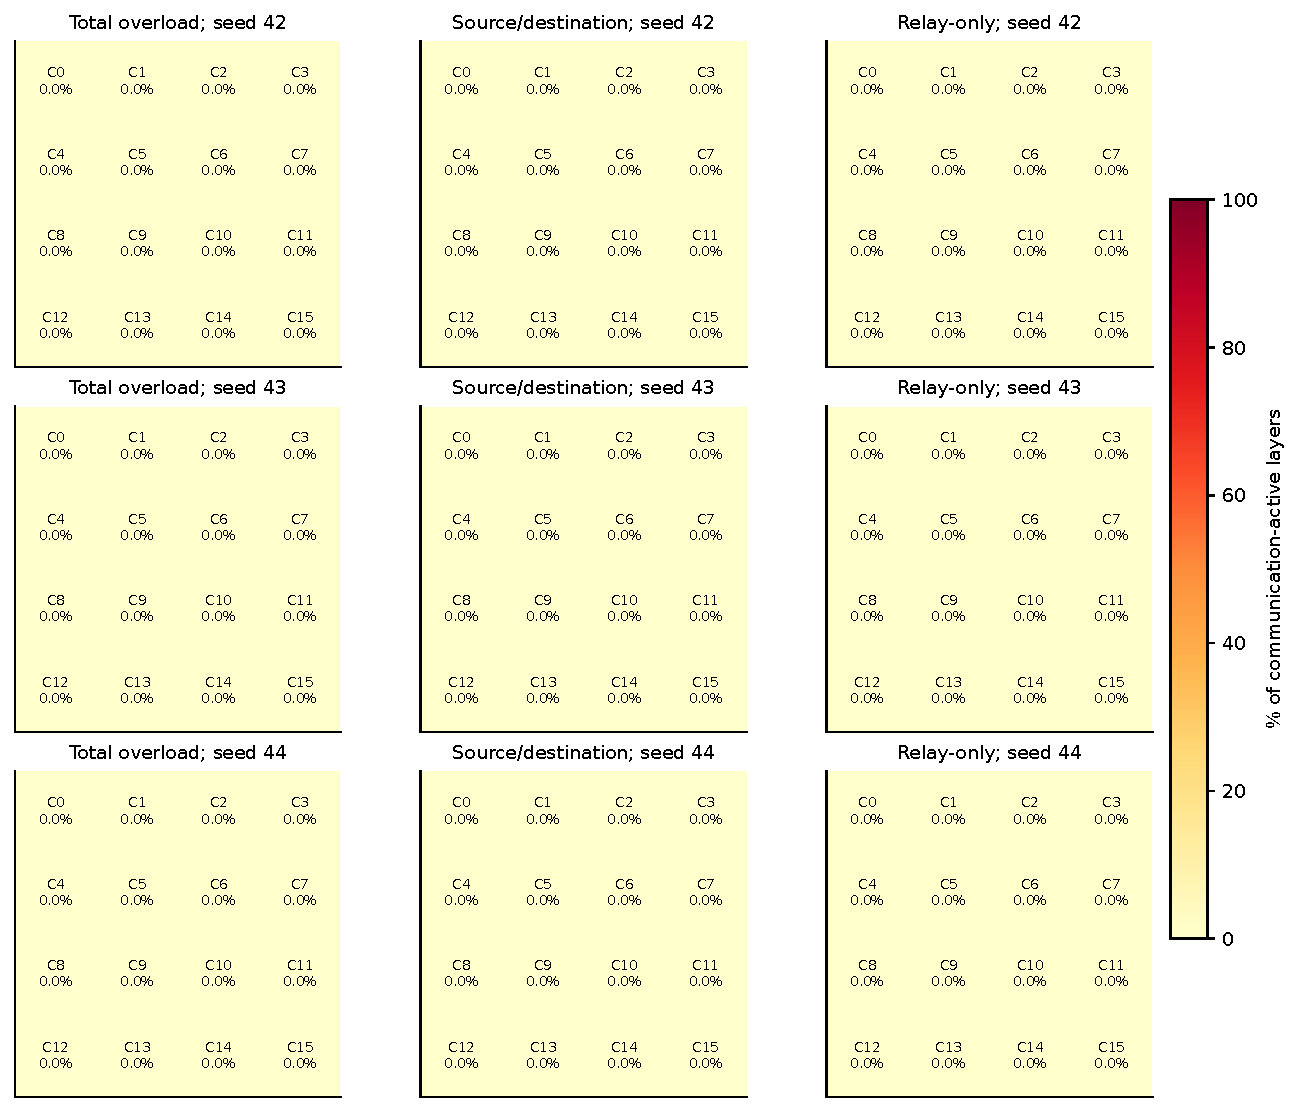
\includegraphics[width=.94\linewidth,height=.48\textheight,keepaspectratio]{figures/atlas/torus_dijkstra_route_m16.pdf}\captionof{figure}{All three conceptual mapping seeds; common 0--100 percent colour scale.}\end{center}
\begin{center}{\scriptsize\setlength{\tabcolsep}{3pt}
\begin{tabular}{lrrrrrrrrr}
\toprule
Core & 42 Tot & 42 Own & 42 Rel & 43 Tot & 43 Own & 43 Rel & 44 Tot & 44 Own & 44 Rel \\
\midrule
0 & 0.000 & 0.000 & 0.000 & 0.000 & 0.000 & 0.000 & 0.000 & 0.000 & 0.000 \\
1 & 0.000 & 0.000 & 0.000 & 0.000 & 0.000 & 0.000 & 0.000 & 0.000 & 0.000 \\
2 & 0.000 & 0.000 & 0.000 & 0.000 & 0.000 & 0.000 & 0.000 & 0.000 & 0.000 \\
3 & 0.000 & 0.000 & 0.000 & 0.000 & 0.000 & 0.000 & 0.000 & 0.000 & 0.000 \\
4 & 0.000 & 0.000 & 0.000 & 0.000 & 0.000 & 0.000 & 0.000 & 0.000 & 0.000 \\
5 & 0.000 & 0.000 & 0.000 & 0.000 & 0.000 & 0.000 & 0.000 & 0.000 & 0.000 \\
6 & 0.000 & 0.000 & 0.000 & 0.000 & 0.000 & 0.000 & 0.000 & 0.000 & 0.000 \\
7 & 0.000 & 0.000 & 0.000 & 0.000 & 0.000 & 0.000 & 0.000 & 0.000 & 0.000 \\
8 & 0.000 & 0.000 & 0.000 & 0.000 & 0.000 & 0.000 & 0.000 & 0.000 & 0.000 \\
9 & 0.000 & 0.000 & 0.000 & 0.000 & 0.000 & 0.000 & 0.000 & 0.000 & 0.000 \\
10 & 0.000 & 0.000 & 0.000 & 0.000 & 0.000 & 0.000 & 0.000 & 0.000 & 0.000 \\
11 & 0.000 & 0.000 & 0.000 & 0.000 & 0.000 & 0.000 & 0.000 & 0.000 & 0.000 \\
12 & 0.000 & 0.000 & 0.000 & 0.000 & 0.000 & 0.000 & 0.000 & 0.000 & 0.000 \\
13 & 0.000 & 0.000 & 0.000 & 0.000 & 0.000 & 0.000 & 0.000 & 0.000 & 0.000 \\
14 & 0.000 & 0.000 & 0.000 & 0.000 & 0.000 & 0.000 & 0.000 & 0.000 & 0.000 \\
15 & 0.000 & 0.000 & 0.000 & 0.000 & 0.000 & 0.000 & 0.000 & 0.000 & 0.000 \\
\bottomrule\end{tabular}}
\captionof{table}{Exact heatmap percentages, with Tot = Own + Rel. Unrounded values are in the CSV.}
{\footnotesize\href{https://github.com/sanjeevkrishnaa/Compiler-Driven-ACE/blob/codex/ace-scheduler-correctness/docs/latex/qft96_final/data/heatmap_torus_dijkstra_route_m16.csv}{Exact CSV values and sample counts}}
\end{center}
\clearpage\subsection*{Torus dijkstra; M=32; route counting}
\begin{center}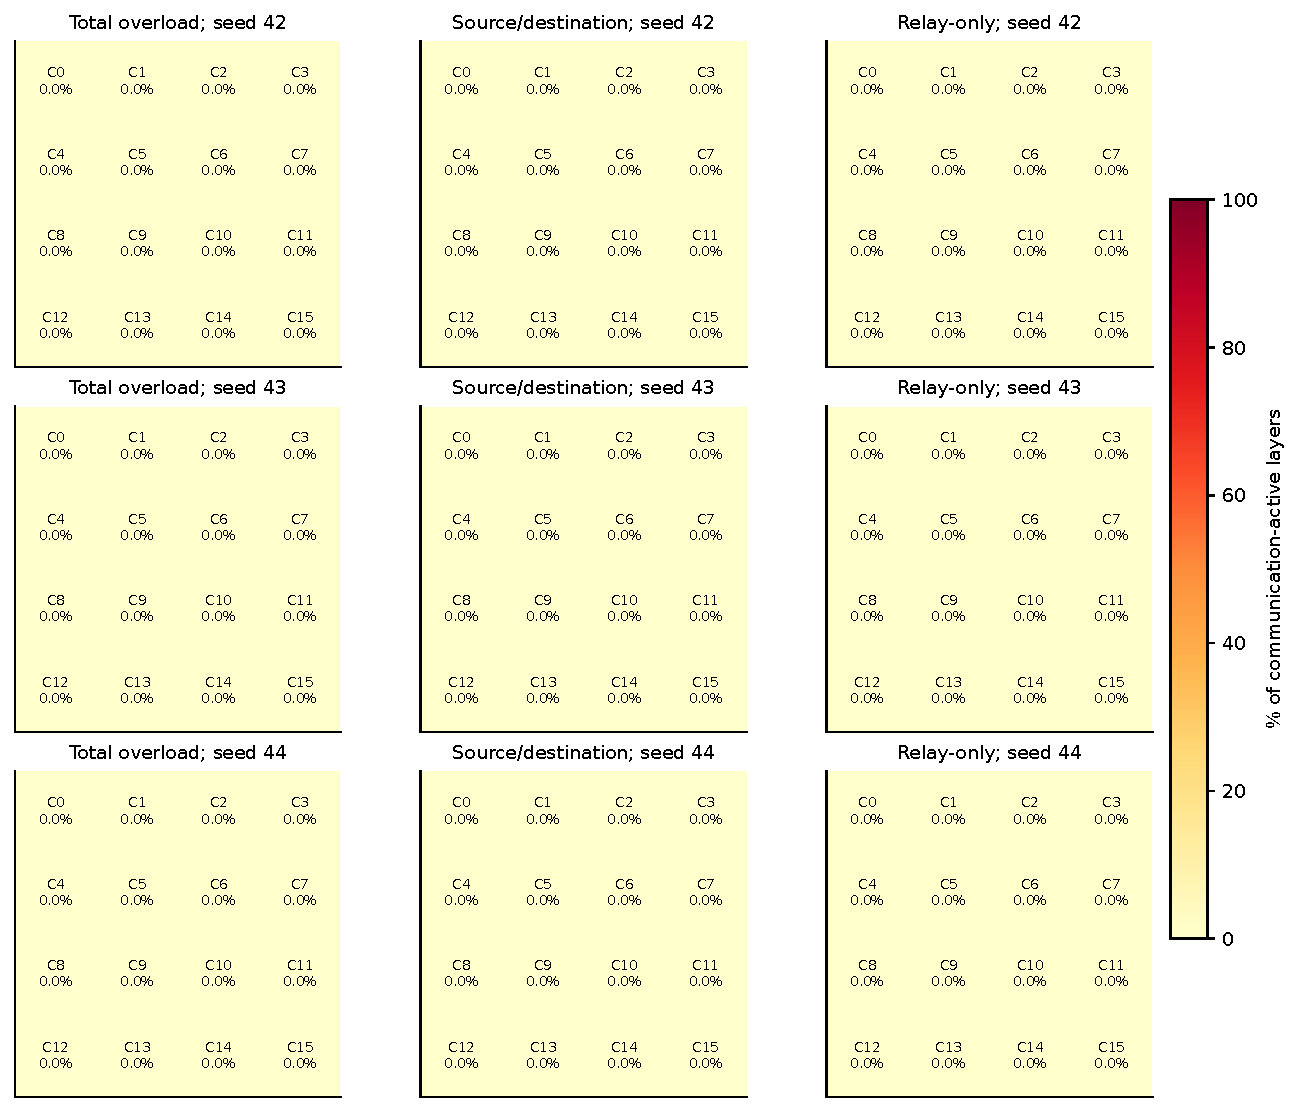
\includegraphics[width=.94\linewidth,height=.48\textheight,keepaspectratio]{figures/atlas/torus_dijkstra_route_m32.pdf}\captionof{figure}{All three conceptual mapping seeds; common 0--100 percent colour scale.}\end{center}
\begin{center}{\scriptsize\setlength{\tabcolsep}{3pt}
\begin{tabular}{lrrrrrrrrr}
\toprule
Core & 42 Tot & 42 Own & 42 Rel & 43 Tot & 43 Own & 43 Rel & 44 Tot & 44 Own & 44 Rel \\
\midrule
0 & 0.000 & 0.000 & 0.000 & 0.000 & 0.000 & 0.000 & 0.000 & 0.000 & 0.000 \\
1 & 0.000 & 0.000 & 0.000 & 0.000 & 0.000 & 0.000 & 0.000 & 0.000 & 0.000 \\
2 & 0.000 & 0.000 & 0.000 & 0.000 & 0.000 & 0.000 & 0.000 & 0.000 & 0.000 \\
3 & 0.000 & 0.000 & 0.000 & 0.000 & 0.000 & 0.000 & 0.000 & 0.000 & 0.000 \\
4 & 0.000 & 0.000 & 0.000 & 0.000 & 0.000 & 0.000 & 0.000 & 0.000 & 0.000 \\
5 & 0.000 & 0.000 & 0.000 & 0.000 & 0.000 & 0.000 & 0.000 & 0.000 & 0.000 \\
6 & 0.000 & 0.000 & 0.000 & 0.000 & 0.000 & 0.000 & 0.000 & 0.000 & 0.000 \\
7 & 0.000 & 0.000 & 0.000 & 0.000 & 0.000 & 0.000 & 0.000 & 0.000 & 0.000 \\
8 & 0.000 & 0.000 & 0.000 & 0.000 & 0.000 & 0.000 & 0.000 & 0.000 & 0.000 \\
9 & 0.000 & 0.000 & 0.000 & 0.000 & 0.000 & 0.000 & 0.000 & 0.000 & 0.000 \\
10 & 0.000 & 0.000 & 0.000 & 0.000 & 0.000 & 0.000 & 0.000 & 0.000 & 0.000 \\
11 & 0.000 & 0.000 & 0.000 & 0.000 & 0.000 & 0.000 & 0.000 & 0.000 & 0.000 \\
12 & 0.000 & 0.000 & 0.000 & 0.000 & 0.000 & 0.000 & 0.000 & 0.000 & 0.000 \\
13 & 0.000 & 0.000 & 0.000 & 0.000 & 0.000 & 0.000 & 0.000 & 0.000 & 0.000 \\
14 & 0.000 & 0.000 & 0.000 & 0.000 & 0.000 & 0.000 & 0.000 & 0.000 & 0.000 \\
15 & 0.000 & 0.000 & 0.000 & 0.000 & 0.000 & 0.000 & 0.000 & 0.000 & 0.000 \\
\bottomrule\end{tabular}}
\captionof{table}{Exact heatmap percentages, with Tot = Own + Rel. Unrounded values are in the CSV.}
{\footnotesize\href{https://github.com/sanjeevkrishnaa/Compiler-Driven-ACE/blob/codex/ace-scheduler-correctness/docs/latex/qft96_final/data/heatmap_torus_dijkstra_route_m32.csv}{Exact CSV values and sample counts}}
\end{center}
\clearpage\subsection*{Torus dijkstra; M=2; hop counting}
\begin{center}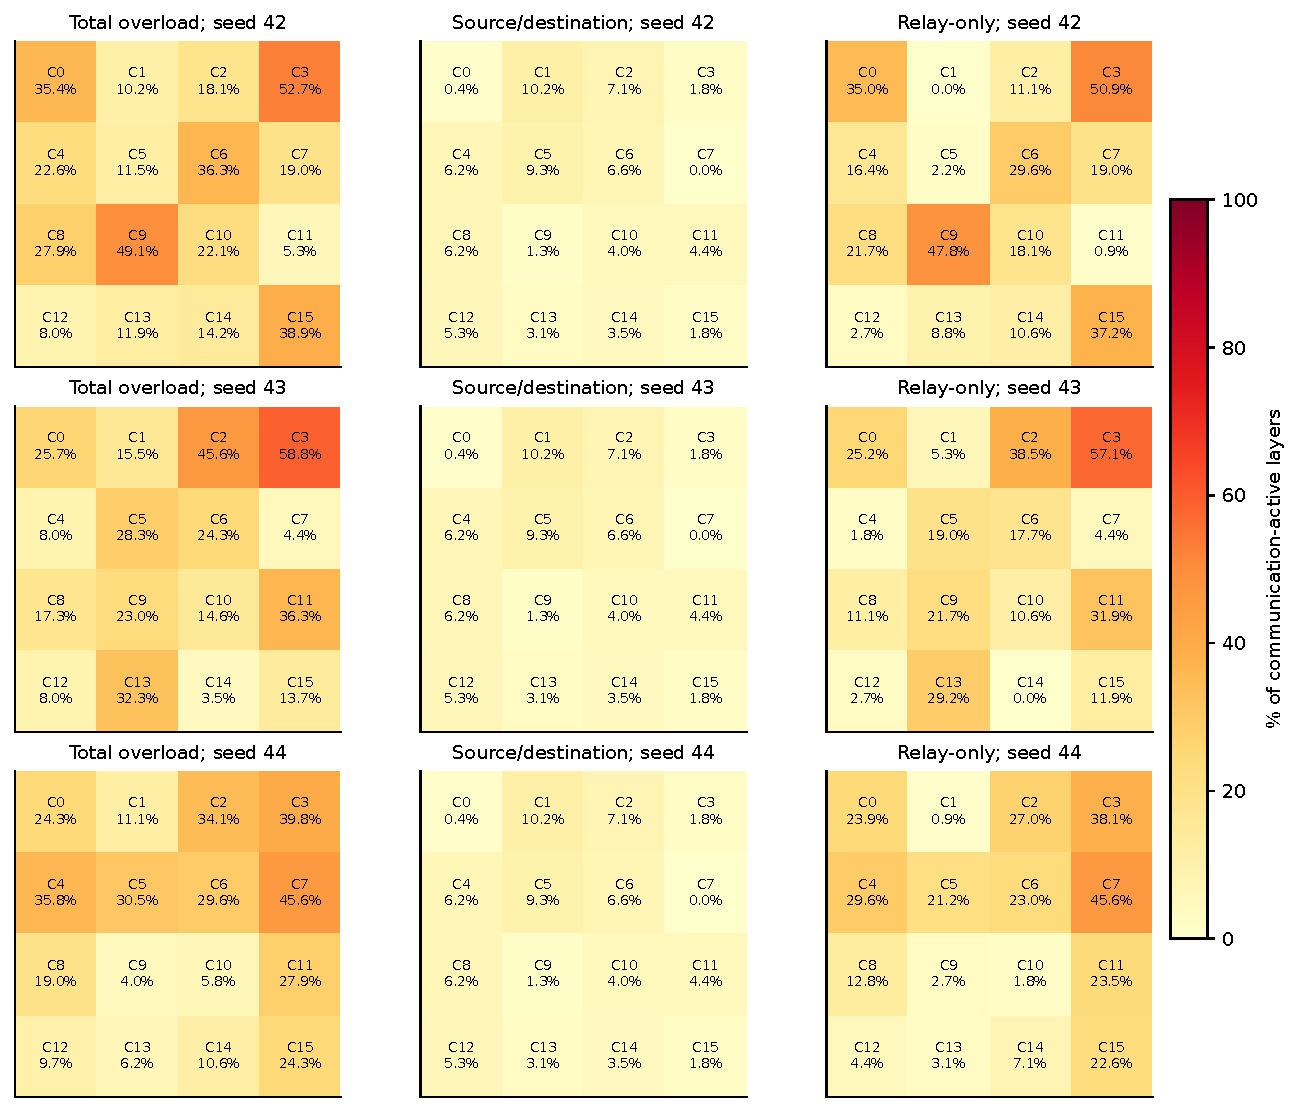
\includegraphics[width=.94\linewidth,height=.48\textheight,keepaspectratio]{figures/atlas/torus_dijkstra_hop_m2.pdf}\captionof{figure}{All three conceptual mapping seeds; common 0--100 percent colour scale.}\end{center}
\begin{center}{\scriptsize\setlength{\tabcolsep}{3pt}
\begin{tabular}{lrrrrrrrrr}
\toprule
Core & 42 Tot & 42 Own & 42 Rel & 43 Tot & 43 Own & 43 Rel & 44 Tot & 44 Own & 44 Rel \\
\midrule
0 & 35.398 & 0.442 & 34.956 & 25.664 & 0.442 & 25.221 & 24.336 & 0.442 & 23.894 \\
1 & 10.177 & 10.177 & 0.000 & 15.487 & 10.177 & 5.310 & 11.062 & 10.177 & 0.885 \\
2 & 18.142 & 7.080 & 11.062 & 45.575 & 7.080 & 38.496 & 34.071 & 7.080 & 26.991 \\
3 & 52.655 & 1.770 & 50.885 & 58.850 & 1.770 & 57.080 & 39.823 & 1.770 & 38.053 \\
4 & 22.566 & 6.195 & 16.372 & 7.965 & 6.195 & 1.770 & 35.841 & 6.195 & 29.646 \\
5 & 11.504 & 9.292 & 2.212 & 28.319 & 9.292 & 19.027 & 30.531 & 9.292 & 21.239 \\
6 & 36.283 & 6.637 & 29.646 & 24.336 & 6.637 & 17.699 & 29.646 & 6.637 & 23.009 \\
7 & 19.027 & 0.000 & 19.027 & 4.425 & 0.000 & 4.425 & 45.575 & 0.000 & 45.575 \\
8 & 27.876 & 6.195 & 21.681 & 17.257 & 6.195 & 11.062 & 19.027 & 6.195 & 12.832 \\
9 & 49.115 & 1.327 & 47.788 & 23.009 & 1.327 & 21.681 & 3.982 & 1.327 & 2.655 \\
10 & 22.124 & 3.982 & 18.142 & 14.602 & 3.982 & 10.619 & 5.752 & 3.982 & 1.770 \\
11 & 5.310 & 4.425 & 0.885 & 36.283 & 4.425 & 31.858 & 27.876 & 4.425 & 23.451 \\
12 & 7.965 & 5.310 & 2.655 & 7.965 & 5.310 & 2.655 & 9.735 & 5.310 & 4.425 \\
13 & 11.947 & 3.097 & 8.850 & 32.301 & 3.097 & 29.204 & 6.195 & 3.097 & 3.097 \\
14 & 14.159 & 3.540 & 10.619 & 3.540 & 3.540 & 0.000 & 10.619 & 3.540 & 7.080 \\
15 & 38.938 & 1.770 & 37.168 & 13.717 & 1.770 & 11.947 & 24.336 & 1.770 & 22.566 \\
\bottomrule\end{tabular}}
\captionof{table}{Exact heatmap percentages, with Tot = Own + Rel. Unrounded values are in the CSV.}
{\footnotesize\href{https://github.com/sanjeevkrishnaa/Compiler-Driven-ACE/blob/codex/ace-scheduler-correctness/docs/latex/qft96_final/data/heatmap_torus_dijkstra_hop_m2.csv}{Exact CSV values and sample counts}}
\end{center}
\clearpage\subsection*{Torus dijkstra; M=3; hop counting}
\begin{center}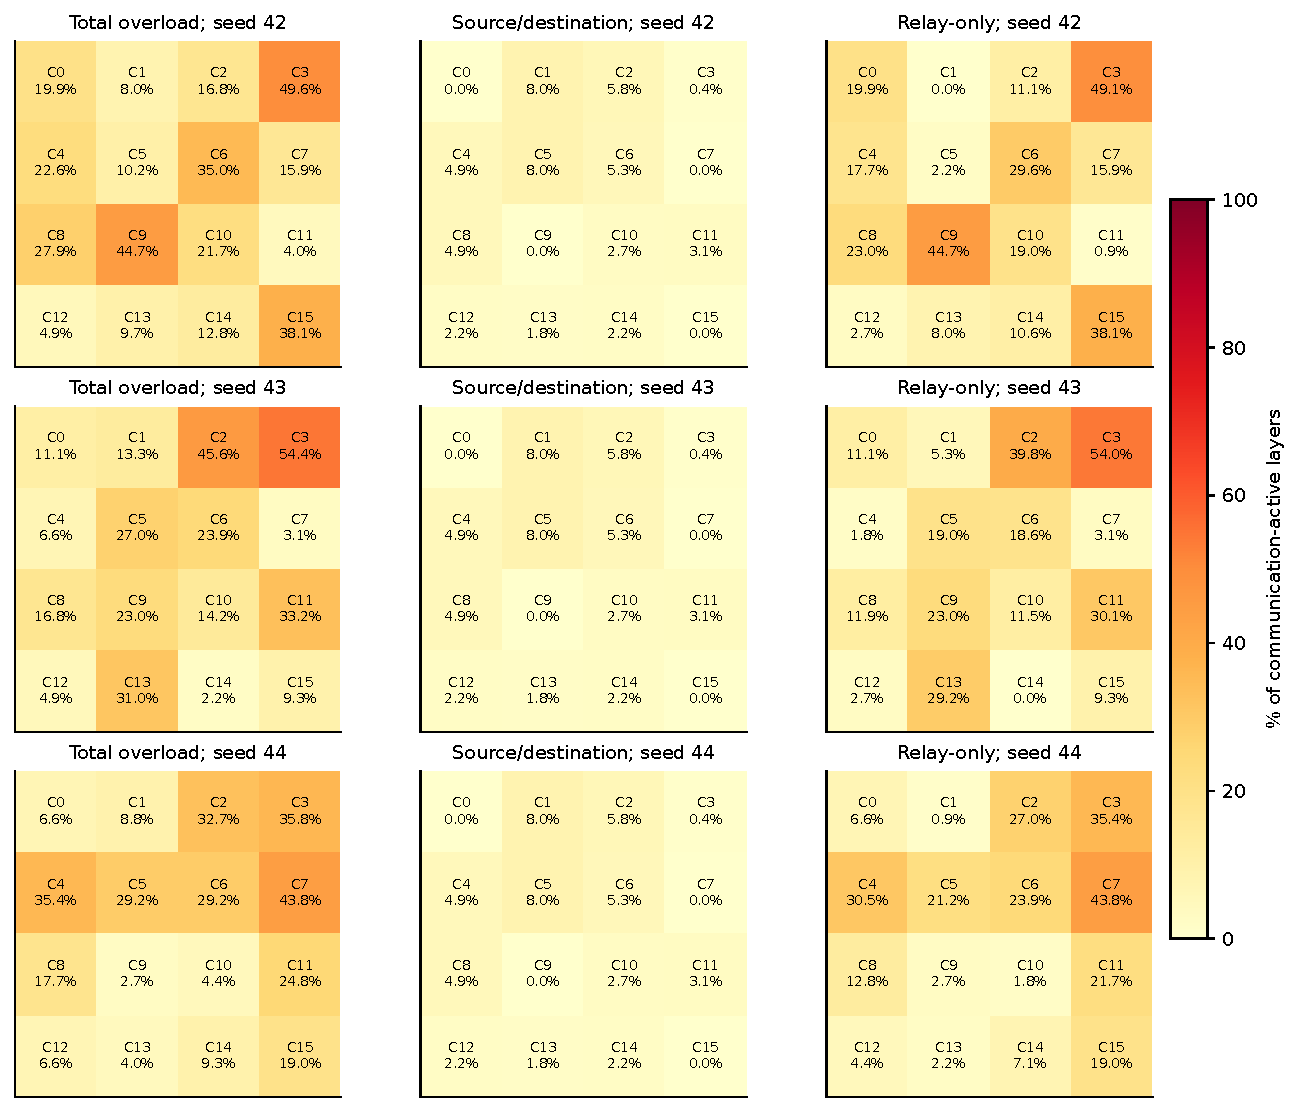
\includegraphics[width=.94\linewidth,height=.48\textheight,keepaspectratio]{figures/atlas/torus_dijkstra_hop_m3.pdf}\captionof{figure}{All three conceptual mapping seeds; common 0--100 percent colour scale.}\end{center}
\begin{center}{\scriptsize\setlength{\tabcolsep}{3pt}
\begin{tabular}{lrrrrrrrrr}
\toprule
Core & 42 Tot & 42 Own & 42 Rel & 43 Tot & 43 Own & 43 Rel & 44 Tot & 44 Own & 44 Rel \\
\midrule
0 & 19.912 & 0.000 & 19.912 & 11.062 & 0.000 & 11.062 & 6.637 & 0.000 & 6.637 \\
1 & 7.965 & 7.965 & 0.000 & 13.274 & 7.965 & 5.310 & 8.850 & 7.965 & 0.885 \\
2 & 16.814 & 5.752 & 11.062 & 45.575 & 5.752 & 39.823 & 32.743 & 5.752 & 26.991 \\
3 & 49.558 & 0.442 & 49.115 & 54.425 & 0.442 & 53.982 & 35.841 & 0.442 & 35.398 \\
4 & 22.566 & 4.867 & 17.699 & 6.637 & 4.867 & 1.770 & 35.398 & 4.867 & 30.531 \\
5 & 10.177 & 7.965 & 2.212 & 26.991 & 7.965 & 19.027 & 29.204 & 7.965 & 21.239 \\
6 & 34.956 & 5.310 & 29.646 & 23.894 & 5.310 & 18.584 & 29.204 & 5.310 & 23.894 \\
7 & 15.929 & 0.000 & 15.929 & 3.097 & 0.000 & 3.097 & 43.805 & 0.000 & 43.805 \\
8 & 27.876 & 4.867 & 23.009 & 16.814 & 4.867 & 11.947 & 17.699 & 4.867 & 12.832 \\
9 & 44.690 & 0.000 & 44.690 & 23.009 & 0.000 & 23.009 & 2.655 & 0.000 & 2.655 \\
10 & 21.681 & 2.655 & 19.027 & 14.159 & 2.655 & 11.504 & 4.425 & 2.655 & 1.770 \\
11 & 3.982 & 3.097 & 0.885 & 33.186 & 3.097 & 30.088 & 24.779 & 3.097 & 21.681 \\
12 & 4.867 & 2.212 & 2.655 & 4.867 & 2.212 & 2.655 & 6.637 & 2.212 & 4.425 \\
13 & 9.735 & 1.770 & 7.965 & 30.973 & 1.770 & 29.204 & 3.982 & 1.770 & 2.212 \\
14 & 12.832 & 2.212 & 10.619 & 2.212 & 2.212 & 0.000 & 9.292 & 2.212 & 7.080 \\
15 & 38.053 & 0.000 & 38.053 & 9.292 & 0.000 & 9.292 & 19.027 & 0.000 & 19.027 \\
\bottomrule\end{tabular}}
\captionof{table}{Exact heatmap percentages, with Tot = Own + Rel. Unrounded values are in the CSV.}
{\footnotesize\href{https://github.com/sanjeevkrishnaa/Compiler-Driven-ACE/blob/codex/ace-scheduler-correctness/docs/latex/qft96_final/data/heatmap_torus_dijkstra_hop_m3.csv}{Exact CSV values and sample counts}}
\end{center}
\clearpage\subsection*{Torus dijkstra; M=4; hop counting}
\begin{center}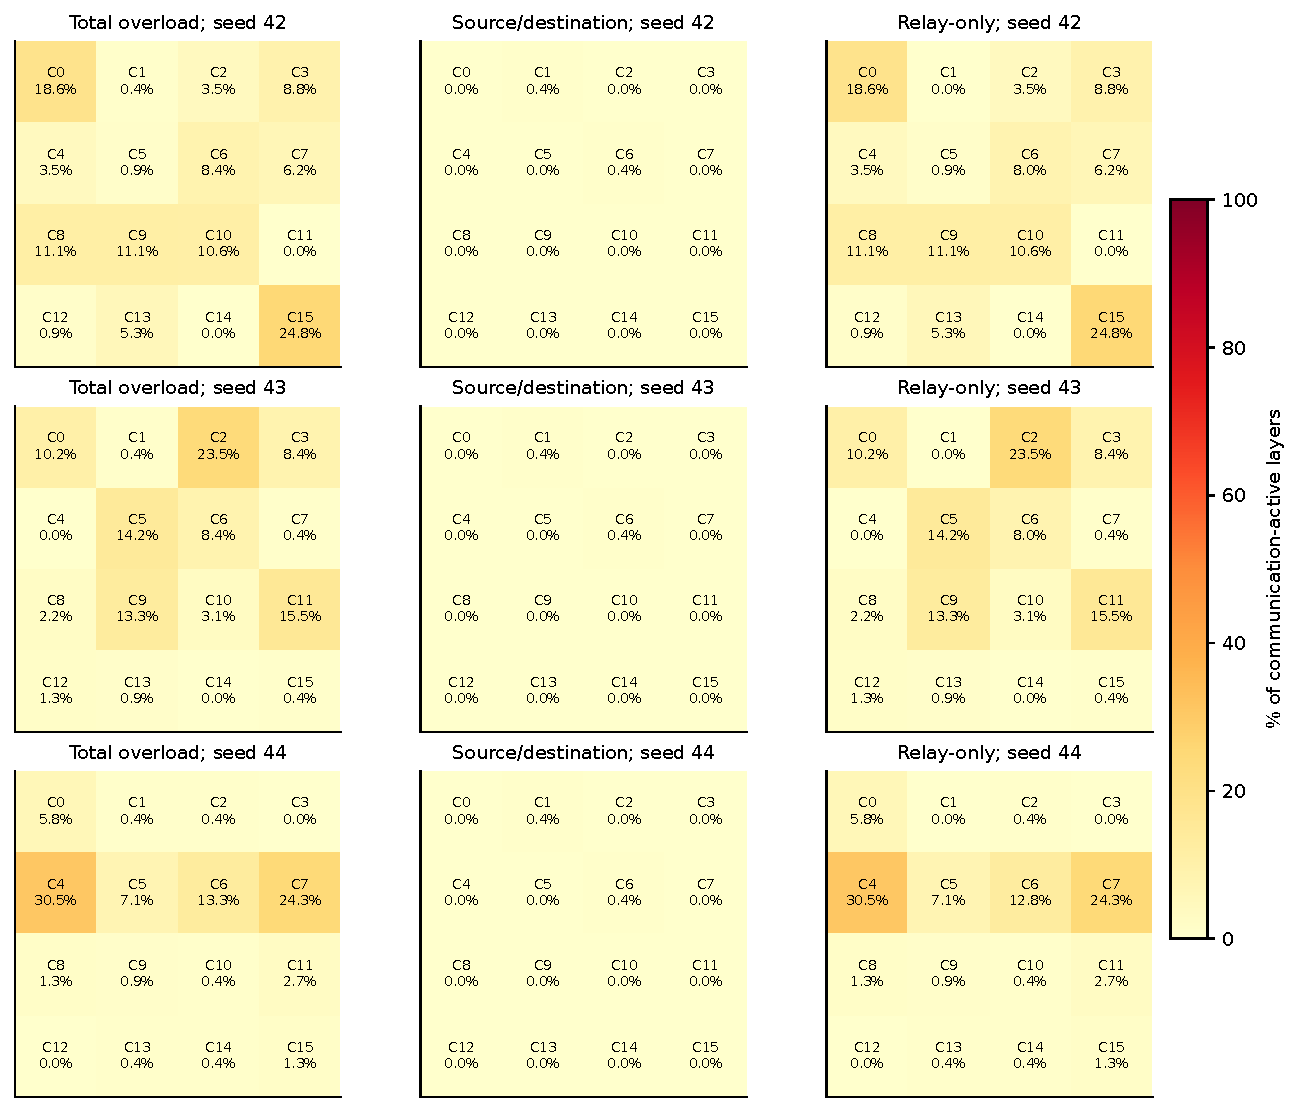
\includegraphics[width=.94\linewidth,height=.48\textheight,keepaspectratio]{figures/atlas/torus_dijkstra_hop_m4.pdf}\captionof{figure}{All three conceptual mapping seeds; common 0--100 percent colour scale.}\end{center}
\begin{center}{\scriptsize\setlength{\tabcolsep}{3pt}
\begin{tabular}{lrrrrrrrrr}
\toprule
Core & 42 Tot & 42 Own & 42 Rel & 43 Tot & 43 Own & 43 Rel & 44 Tot & 44 Own & 44 Rel \\
\midrule
0 & 18.584 & 0.000 & 18.584 & 10.177 & 0.000 & 10.177 & 5.752 & 0.000 & 5.752 \\
1 & 0.442 & 0.442 & 0.000 & 0.442 & 0.442 & 0.000 & 0.442 & 0.442 & 0.000 \\
2 & 3.540 & 0.000 & 3.540 & 23.451 & 0.000 & 23.451 & 0.442 & 0.000 & 0.442 \\
3 & 8.850 & 0.000 & 8.850 & 8.407 & 0.000 & 8.407 & 0.000 & 0.000 & 0.000 \\
4 & 3.540 & 0.000 & 3.540 & 0.000 & 0.000 & 0.000 & 30.531 & 0.000 & 30.531 \\
5 & 0.885 & 0.000 & 0.885 & 14.159 & 0.000 & 14.159 & 7.080 & 0.000 & 7.080 \\
6 & 8.407 & 0.442 & 7.965 & 8.407 & 0.442 & 7.965 & 13.274 & 0.442 & 12.832 \\
7 & 6.195 & 0.000 & 6.195 & 0.442 & 0.000 & 0.442 & 24.336 & 0.000 & 24.336 \\
8 & 11.062 & 0.000 & 11.062 & 2.212 & 0.000 & 2.212 & 1.327 & 0.000 & 1.327 \\
9 & 11.062 & 0.000 & 11.062 & 13.274 & 0.000 & 13.274 & 0.885 & 0.000 & 0.885 \\
10 & 10.619 & 0.000 & 10.619 & 3.097 & 0.000 & 3.097 & 0.442 & 0.000 & 0.442 \\
11 & 0.000 & 0.000 & 0.000 & 15.487 & 0.000 & 15.487 & 2.655 & 0.000 & 2.655 \\
12 & 0.885 & 0.000 & 0.885 & 1.327 & 0.000 & 1.327 & 0.000 & 0.000 & 0.000 \\
13 & 5.310 & 0.000 & 5.310 & 0.885 & 0.000 & 0.885 & 0.442 & 0.000 & 0.442 \\
14 & 0.000 & 0.000 & 0.000 & 0.000 & 0.000 & 0.000 & 0.442 & 0.000 & 0.442 \\
15 & 24.779 & 0.000 & 24.779 & 0.442 & 0.000 & 0.442 & 1.327 & 0.000 & 1.327 \\
\bottomrule\end{tabular}}
\captionof{table}{Exact heatmap percentages, with Tot = Own + Rel. Unrounded values are in the CSV.}
{\footnotesize\href{https://github.com/sanjeevkrishnaa/Compiler-Driven-ACE/blob/codex/ace-scheduler-correctness/docs/latex/qft96_final/data/heatmap_torus_dijkstra_hop_m4.csv}{Exact CSV values and sample counts}}
\end{center}
\clearpage\subsection*{Torus dijkstra; M=6; hop counting}
\begin{center}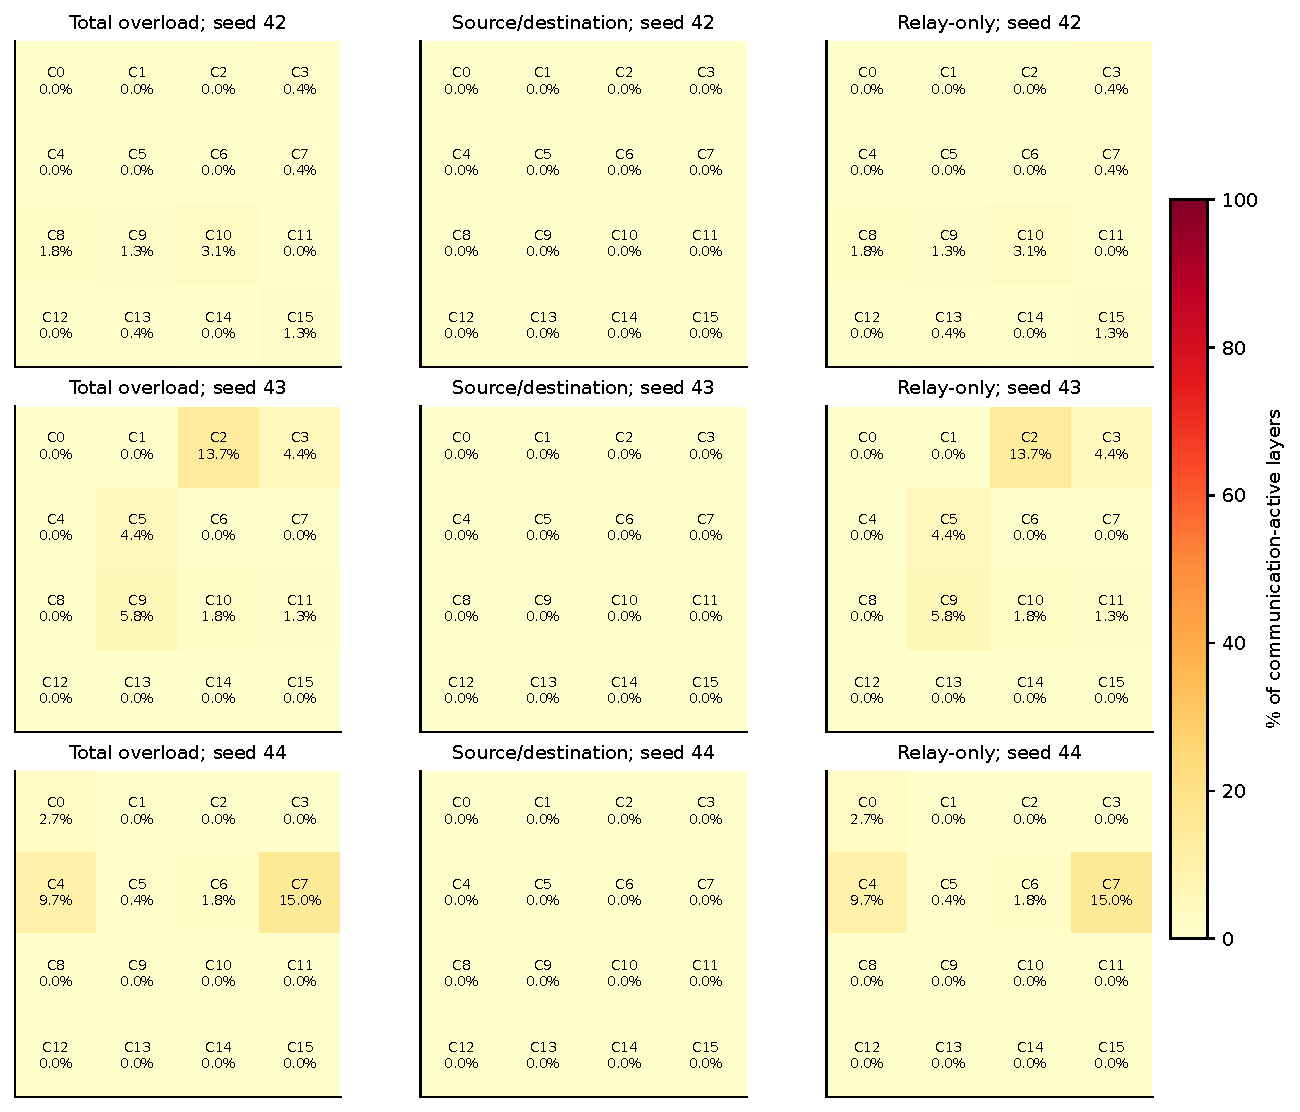
\includegraphics[width=.94\linewidth,height=.48\textheight,keepaspectratio]{figures/atlas/torus_dijkstra_hop_m6.pdf}\captionof{figure}{All three conceptual mapping seeds; common 0--100 percent colour scale.}\end{center}
\begin{center}{\scriptsize\setlength{\tabcolsep}{3pt}
\begin{tabular}{lrrrrrrrrr}
\toprule
Core & 42 Tot & 42 Own & 42 Rel & 43 Tot & 43 Own & 43 Rel & 44 Tot & 44 Own & 44 Rel \\
\midrule
0 & 0.000 & 0.000 & 0.000 & 0.000 & 0.000 & 0.000 & 2.655 & 0.000 & 2.655 \\
1 & 0.000 & 0.000 & 0.000 & 0.000 & 0.000 & 0.000 & 0.000 & 0.000 & 0.000 \\
2 & 0.000 & 0.000 & 0.000 & 13.717 & 0.000 & 13.717 & 0.000 & 0.000 & 0.000 \\
3 & 0.442 & 0.000 & 0.442 & 4.425 & 0.000 & 4.425 & 0.000 & 0.000 & 0.000 \\
4 & 0.000 & 0.000 & 0.000 & 0.000 & 0.000 & 0.000 & 9.735 & 0.000 & 9.735 \\
5 & 0.000 & 0.000 & 0.000 & 4.425 & 0.000 & 4.425 & 0.442 & 0.000 & 0.442 \\
6 & 0.000 & 0.000 & 0.000 & 0.000 & 0.000 & 0.000 & 1.770 & 0.000 & 1.770 \\
7 & 0.442 & 0.000 & 0.442 & 0.000 & 0.000 & 0.000 & 15.044 & 0.000 & 15.044 \\
8 & 1.770 & 0.000 & 1.770 & 0.000 & 0.000 & 0.000 & 0.000 & 0.000 & 0.000 \\
9 & 1.327 & 0.000 & 1.327 & 5.752 & 0.000 & 5.752 & 0.000 & 0.000 & 0.000 \\
10 & 3.097 & 0.000 & 3.097 & 1.770 & 0.000 & 1.770 & 0.000 & 0.000 & 0.000 \\
11 & 0.000 & 0.000 & 0.000 & 1.327 & 0.000 & 1.327 & 0.000 & 0.000 & 0.000 \\
12 & 0.000 & 0.000 & 0.000 & 0.000 & 0.000 & 0.000 & 0.000 & 0.000 & 0.000 \\
13 & 0.442 & 0.000 & 0.442 & 0.000 & 0.000 & 0.000 & 0.000 & 0.000 & 0.000 \\
14 & 0.000 & 0.000 & 0.000 & 0.000 & 0.000 & 0.000 & 0.000 & 0.000 & 0.000 \\
15 & 1.327 & 0.000 & 1.327 & 0.000 & 0.000 & 0.000 & 0.000 & 0.000 & 0.000 \\
\bottomrule\end{tabular}}
\captionof{table}{Exact heatmap percentages, with Tot = Own + Rel. Unrounded values are in the CSV.}
{\footnotesize\href{https://github.com/sanjeevkrishnaa/Compiler-Driven-ACE/blob/codex/ace-scheduler-correctness/docs/latex/qft96_final/data/heatmap_torus_dijkstra_hop_m6.csv}{Exact CSV values and sample counts}}
\end{center}
\clearpage\subsection*{Torus dijkstra; M=8; hop counting}
\begin{center}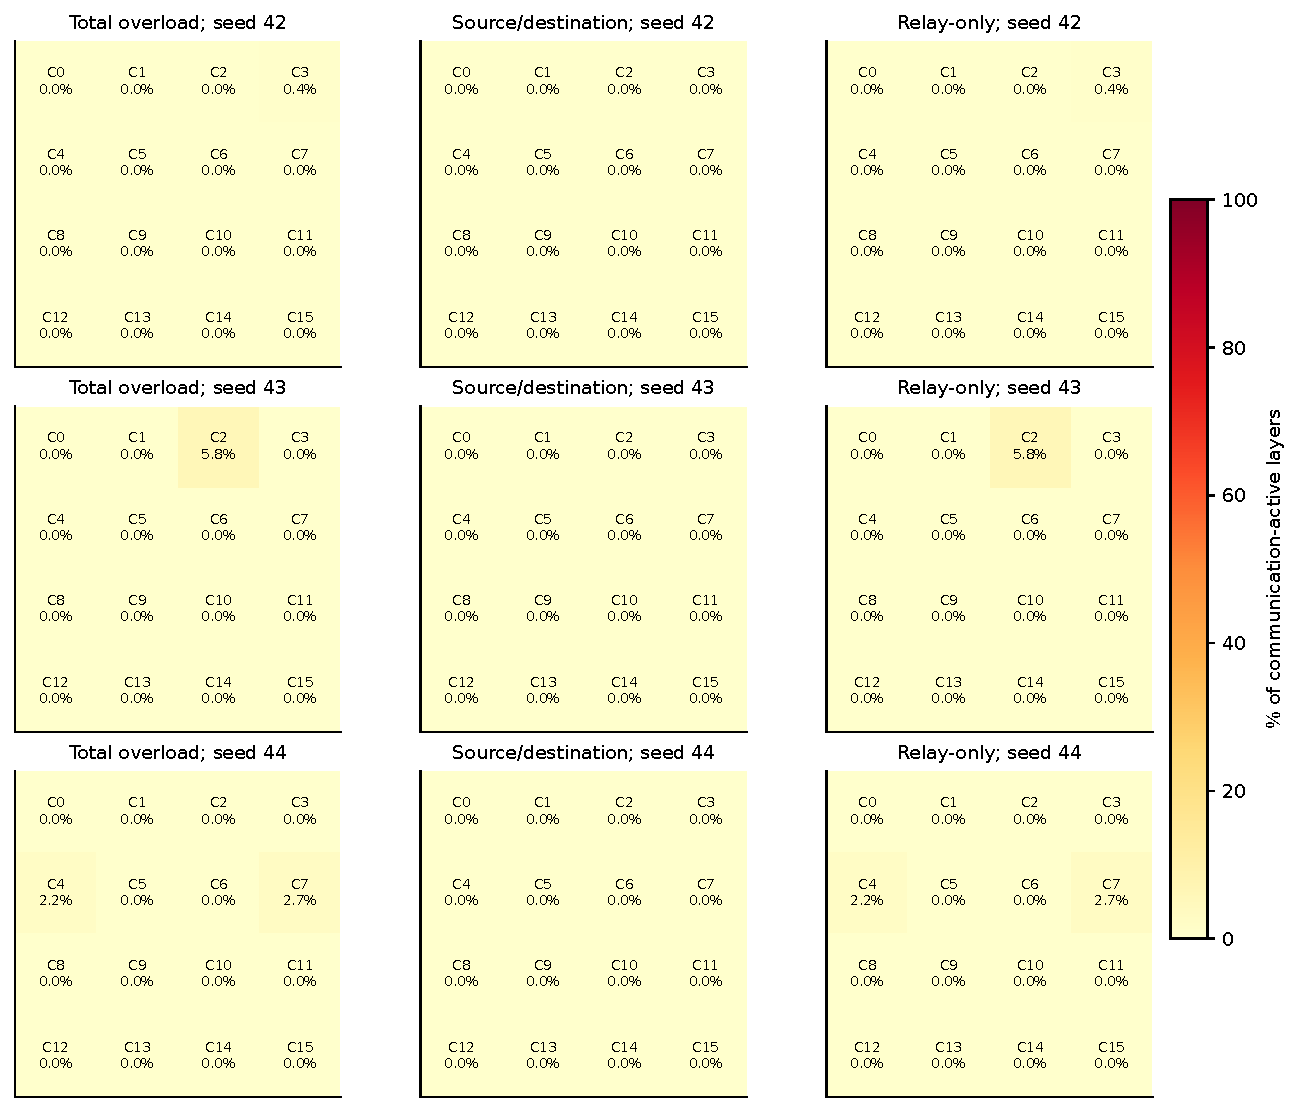
\includegraphics[width=.94\linewidth,height=.48\textheight,keepaspectratio]{figures/atlas/torus_dijkstra_hop_m8.pdf}\captionof{figure}{All three conceptual mapping seeds; common 0--100 percent colour scale.}\end{center}
\begin{center}{\scriptsize\setlength{\tabcolsep}{3pt}
\begin{tabular}{lrrrrrrrrr}
\toprule
Core & 42 Tot & 42 Own & 42 Rel & 43 Tot & 43 Own & 43 Rel & 44 Tot & 44 Own & 44 Rel \\
\midrule
0 & 0.000 & 0.000 & 0.000 & 0.000 & 0.000 & 0.000 & 0.000 & 0.000 & 0.000 \\
1 & 0.000 & 0.000 & 0.000 & 0.000 & 0.000 & 0.000 & 0.000 & 0.000 & 0.000 \\
2 & 0.000 & 0.000 & 0.000 & 5.752 & 0.000 & 5.752 & 0.000 & 0.000 & 0.000 \\
3 & 0.442 & 0.000 & 0.442 & 0.000 & 0.000 & 0.000 & 0.000 & 0.000 & 0.000 \\
4 & 0.000 & 0.000 & 0.000 & 0.000 & 0.000 & 0.000 & 2.212 & 0.000 & 2.212 \\
5 & 0.000 & 0.000 & 0.000 & 0.000 & 0.000 & 0.000 & 0.000 & 0.000 & 0.000 \\
6 & 0.000 & 0.000 & 0.000 & 0.000 & 0.000 & 0.000 & 0.000 & 0.000 & 0.000 \\
7 & 0.000 & 0.000 & 0.000 & 0.000 & 0.000 & 0.000 & 2.655 & 0.000 & 2.655 \\
8 & 0.000 & 0.000 & 0.000 & 0.000 & 0.000 & 0.000 & 0.000 & 0.000 & 0.000 \\
9 & 0.000 & 0.000 & 0.000 & 0.000 & 0.000 & 0.000 & 0.000 & 0.000 & 0.000 \\
10 & 0.000 & 0.000 & 0.000 & 0.000 & 0.000 & 0.000 & 0.000 & 0.000 & 0.000 \\
11 & 0.000 & 0.000 & 0.000 & 0.000 & 0.000 & 0.000 & 0.000 & 0.000 & 0.000 \\
12 & 0.000 & 0.000 & 0.000 & 0.000 & 0.000 & 0.000 & 0.000 & 0.000 & 0.000 \\
13 & 0.000 & 0.000 & 0.000 & 0.000 & 0.000 & 0.000 & 0.000 & 0.000 & 0.000 \\
14 & 0.000 & 0.000 & 0.000 & 0.000 & 0.000 & 0.000 & 0.000 & 0.000 & 0.000 \\
15 & 0.000 & 0.000 & 0.000 & 0.000 & 0.000 & 0.000 & 0.000 & 0.000 & 0.000 \\
\bottomrule\end{tabular}}
\captionof{table}{Exact heatmap percentages, with Tot = Own + Rel. Unrounded values are in the CSV.}
{\footnotesize\href{https://github.com/sanjeevkrishnaa/Compiler-Driven-ACE/blob/codex/ace-scheduler-correctness/docs/latex/qft96_final/data/heatmap_torus_dijkstra_hop_m8.csv}{Exact CSV values and sample counts}}
\end{center}
\clearpage\subsection*{Torus dijkstra; M=16; hop counting}
\begin{center}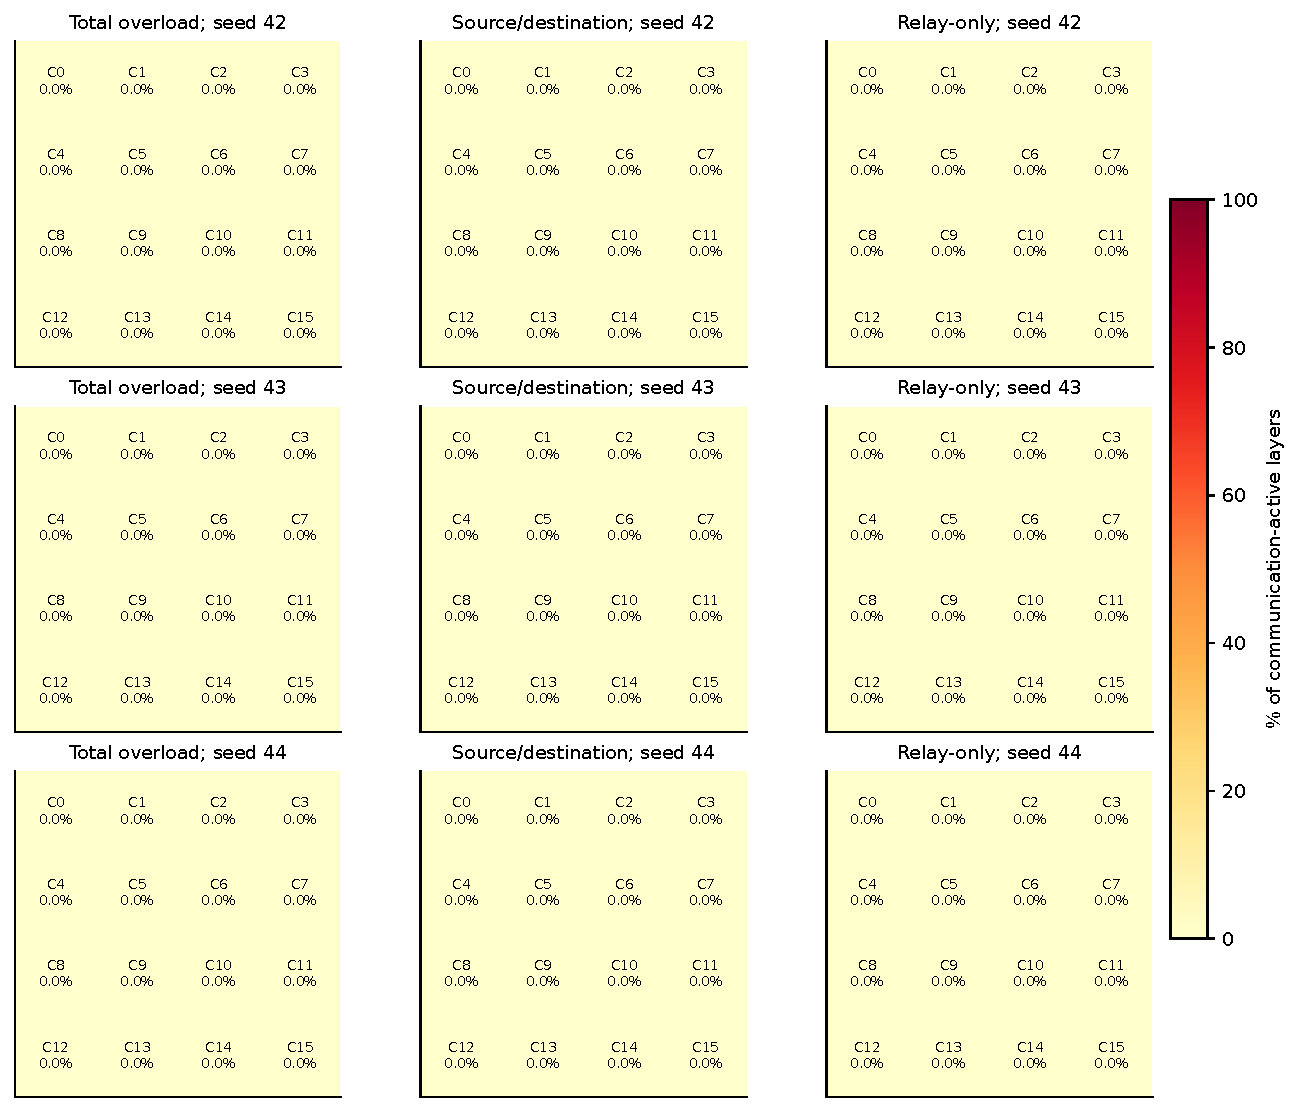
\includegraphics[width=.94\linewidth,height=.48\textheight,keepaspectratio]{figures/atlas/torus_dijkstra_hop_m16.pdf}\captionof{figure}{All three conceptual mapping seeds; common 0--100 percent colour scale.}\end{center}
\begin{center}{\scriptsize\setlength{\tabcolsep}{3pt}
\begin{tabular}{lrrrrrrrrr}
\toprule
Core & 42 Tot & 42 Own & 42 Rel & 43 Tot & 43 Own & 43 Rel & 44 Tot & 44 Own & 44 Rel \\
\midrule
0 & 0.000 & 0.000 & 0.000 & 0.000 & 0.000 & 0.000 & 0.000 & 0.000 & 0.000 \\
1 & 0.000 & 0.000 & 0.000 & 0.000 & 0.000 & 0.000 & 0.000 & 0.000 & 0.000 \\
2 & 0.000 & 0.000 & 0.000 & 0.000 & 0.000 & 0.000 & 0.000 & 0.000 & 0.000 \\
3 & 0.000 & 0.000 & 0.000 & 0.000 & 0.000 & 0.000 & 0.000 & 0.000 & 0.000 \\
4 & 0.000 & 0.000 & 0.000 & 0.000 & 0.000 & 0.000 & 0.000 & 0.000 & 0.000 \\
5 & 0.000 & 0.000 & 0.000 & 0.000 & 0.000 & 0.000 & 0.000 & 0.000 & 0.000 \\
6 & 0.000 & 0.000 & 0.000 & 0.000 & 0.000 & 0.000 & 0.000 & 0.000 & 0.000 \\
7 & 0.000 & 0.000 & 0.000 & 0.000 & 0.000 & 0.000 & 0.000 & 0.000 & 0.000 \\
8 & 0.000 & 0.000 & 0.000 & 0.000 & 0.000 & 0.000 & 0.000 & 0.000 & 0.000 \\
9 & 0.000 & 0.000 & 0.000 & 0.000 & 0.000 & 0.000 & 0.000 & 0.000 & 0.000 \\
10 & 0.000 & 0.000 & 0.000 & 0.000 & 0.000 & 0.000 & 0.000 & 0.000 & 0.000 \\
11 & 0.000 & 0.000 & 0.000 & 0.000 & 0.000 & 0.000 & 0.000 & 0.000 & 0.000 \\
12 & 0.000 & 0.000 & 0.000 & 0.000 & 0.000 & 0.000 & 0.000 & 0.000 & 0.000 \\
13 & 0.000 & 0.000 & 0.000 & 0.000 & 0.000 & 0.000 & 0.000 & 0.000 & 0.000 \\
14 & 0.000 & 0.000 & 0.000 & 0.000 & 0.000 & 0.000 & 0.000 & 0.000 & 0.000 \\
15 & 0.000 & 0.000 & 0.000 & 0.000 & 0.000 & 0.000 & 0.000 & 0.000 & 0.000 \\
\bottomrule\end{tabular}}
\captionof{table}{Exact heatmap percentages, with Tot = Own + Rel. Unrounded values are in the CSV.}
{\footnotesize\href{https://github.com/sanjeevkrishnaa/Compiler-Driven-ACE/blob/codex/ace-scheduler-correctness/docs/latex/qft96_final/data/heatmap_torus_dijkstra_hop_m16.csv}{Exact CSV values and sample counts}}
\end{center}
\clearpage\subsection*{Torus dijkstra; M=32; hop counting}
\begin{center}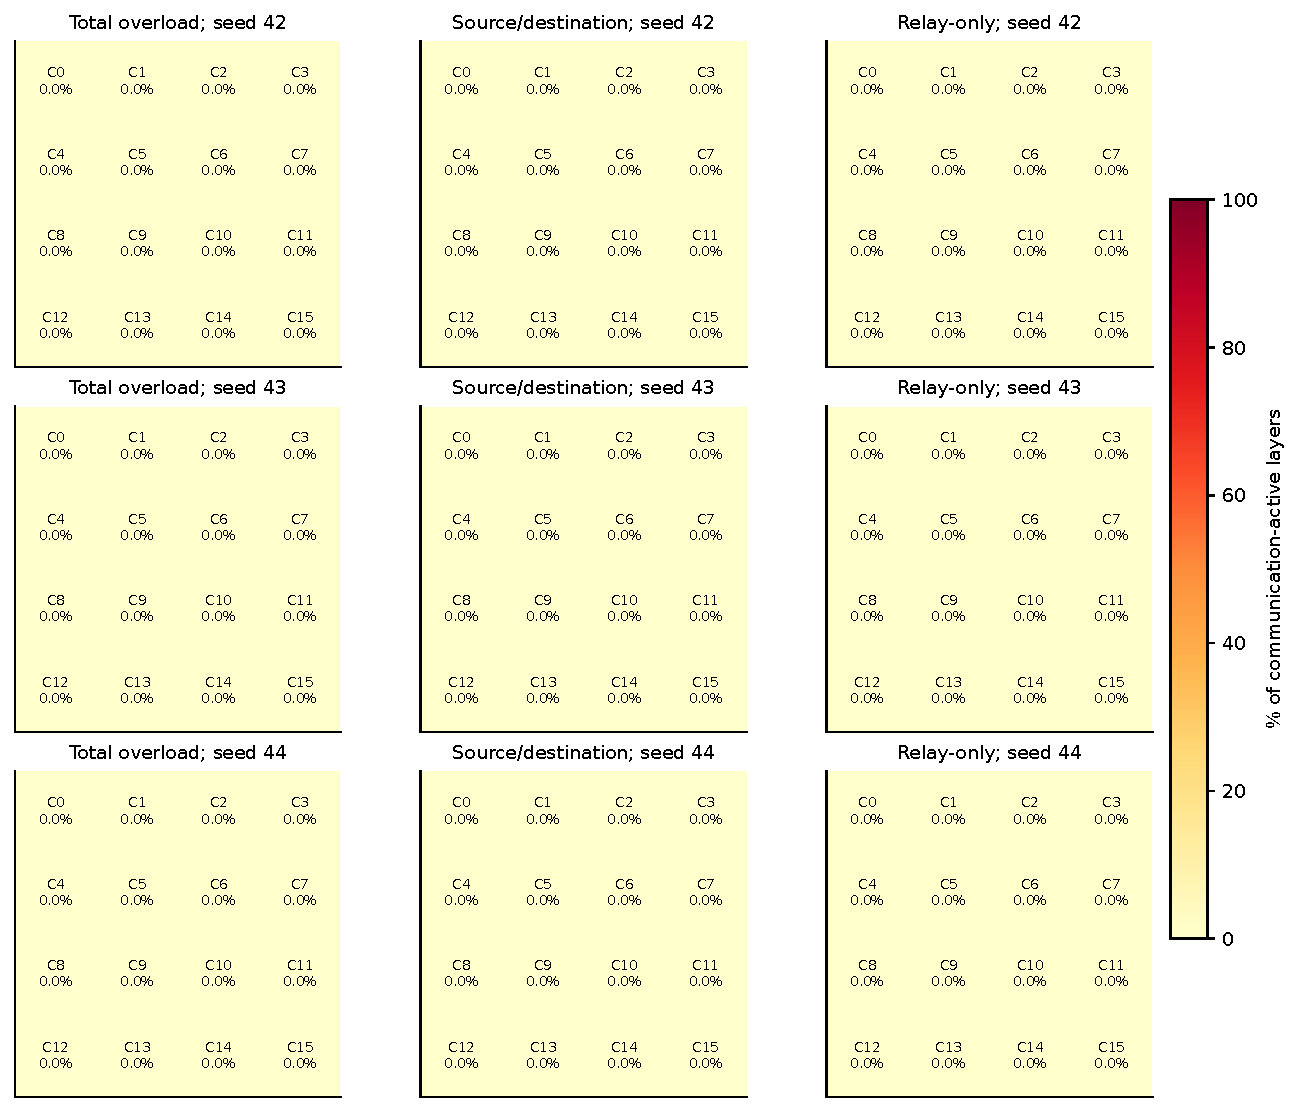
\includegraphics[width=.94\linewidth,height=.48\textheight,keepaspectratio]{figures/atlas/torus_dijkstra_hop_m32.pdf}\captionof{figure}{All three conceptual mapping seeds; common 0--100 percent colour scale.}\end{center}
\begin{center}{\scriptsize\setlength{\tabcolsep}{3pt}
\begin{tabular}{lrrrrrrrrr}
\toprule
Core & 42 Tot & 42 Own & 42 Rel & 43 Tot & 43 Own & 43 Rel & 44 Tot & 44 Own & 44 Rel \\
\midrule
0 & 0.000 & 0.000 & 0.000 & 0.000 & 0.000 & 0.000 & 0.000 & 0.000 & 0.000 \\
1 & 0.000 & 0.000 & 0.000 & 0.000 & 0.000 & 0.000 & 0.000 & 0.000 & 0.000 \\
2 & 0.000 & 0.000 & 0.000 & 0.000 & 0.000 & 0.000 & 0.000 & 0.000 & 0.000 \\
3 & 0.000 & 0.000 & 0.000 & 0.000 & 0.000 & 0.000 & 0.000 & 0.000 & 0.000 \\
4 & 0.000 & 0.000 & 0.000 & 0.000 & 0.000 & 0.000 & 0.000 & 0.000 & 0.000 \\
5 & 0.000 & 0.000 & 0.000 & 0.000 & 0.000 & 0.000 & 0.000 & 0.000 & 0.000 \\
6 & 0.000 & 0.000 & 0.000 & 0.000 & 0.000 & 0.000 & 0.000 & 0.000 & 0.000 \\
7 & 0.000 & 0.000 & 0.000 & 0.000 & 0.000 & 0.000 & 0.000 & 0.000 & 0.000 \\
8 & 0.000 & 0.000 & 0.000 & 0.000 & 0.000 & 0.000 & 0.000 & 0.000 & 0.000 \\
9 & 0.000 & 0.000 & 0.000 & 0.000 & 0.000 & 0.000 & 0.000 & 0.000 & 0.000 \\
10 & 0.000 & 0.000 & 0.000 & 0.000 & 0.000 & 0.000 & 0.000 & 0.000 & 0.000 \\
11 & 0.000 & 0.000 & 0.000 & 0.000 & 0.000 & 0.000 & 0.000 & 0.000 & 0.000 \\
12 & 0.000 & 0.000 & 0.000 & 0.000 & 0.000 & 0.000 & 0.000 & 0.000 & 0.000 \\
13 & 0.000 & 0.000 & 0.000 & 0.000 & 0.000 & 0.000 & 0.000 & 0.000 & 0.000 \\
14 & 0.000 & 0.000 & 0.000 & 0.000 & 0.000 & 0.000 & 0.000 & 0.000 & 0.000 \\
15 & 0.000 & 0.000 & 0.000 & 0.000 & 0.000 & 0.000 & 0.000 & 0.000 & 0.000 \\
\bottomrule\end{tabular}}
\captionof{table}{Exact heatmap percentages, with Tot = Own + Rel. Unrounded values are in the CSV.}
{\footnotesize\href{https://github.com/sanjeevkrishnaa/Compiler-Driven-ACE/blob/codex/ace-scheduler-correctness/docs/latex/qft96_final/data/heatmap_torus_dijkstra_hop_m32.csv}{Exact CSV values and sample counts}}
\end{center}

\chapter{Mesh: routing-specific memory and policy results}
This chapter begins with latency and follows the same metric order for XY, YX, shortest-reliable and maximum-reliability. Each graph uses total communication memories per core on the horizontal axis and includes all instrumented base policies. Its immediate table provides the exact values and a committed CSV link. All 47 registered outcomes and diagnostic metrics are retained.

XY changes dimension 0 first (row first in the repository's coordinate convention); YX changes dimension 1 first. Shortest-reliable minimises hops and then maximises path reliability. Maximum-reliability maximises the product of link reliabilities, with hop count as a secondary criterion, so it can generate extra hops. Mapper reliability selects paths; these comparisons do not establish a calibrated heterogeneous physical link-success model.

All curves use ODG $C=0$ and cached methods $C=M-1$, with $G=\max(1,C)$. Compiler-specific readiness or waste is n/a for ODG/CGP/ACGP rather than being portrayed as a measured autonomous-cache hit statistic. The native protocol measurements are shown separately. Figure error bars are sample SD, with exact observation counts in each CSV.
\section{XY}
\clearpage
\subsection*{Mean request latency}
\begin{center}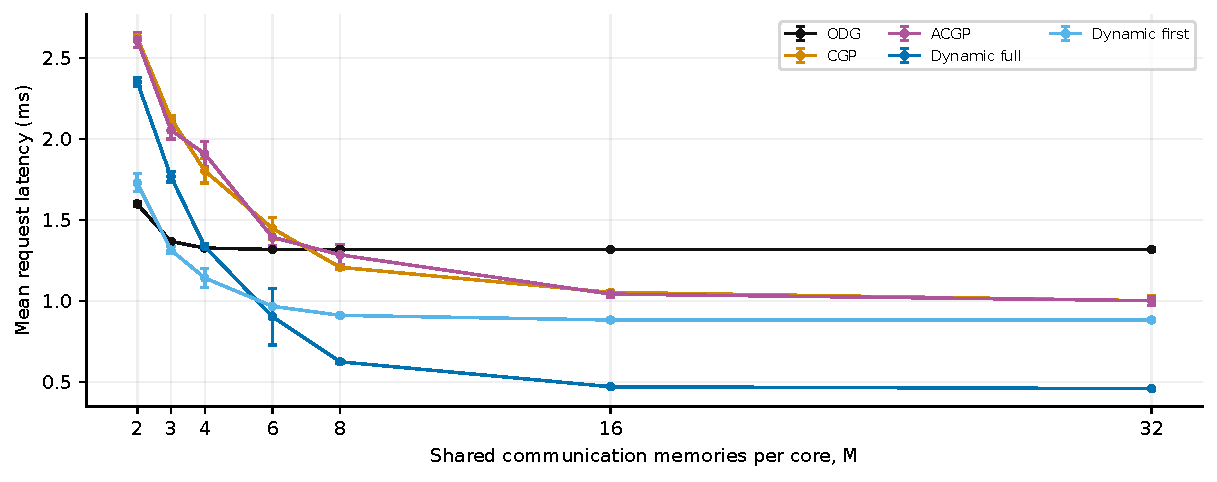
\includegraphics[width=.94\linewidth,height=.255\textheight,keepaspectratio]{figures/memory/mesh_xy_request_latency_mean_ms.pdf}\captionof{figure}{Run-level mean and sample SD. Shared trace aliases are counted once.}\end{center}
\begin{center}{\scriptsize\setlength{\tabcolsep}{3pt}
\begin{tabular}{lrrrrr}
\toprule
M & ODG & CGP & ACGP & Dynamic full & Dynamic first \\
\midrule
2 & $1.599\pm0.016$ & $2.625\pm0.000$ & $2.612\pm0.046$ & $2.353\pm0.026$ & $1.729\pm0.055$ \\
3 & $1.367\pm0.008$ & $2.126\pm0.020$ & $2.054\pm0.054$ & $1.766\pm0.032$ & $1.314\pm0.022$ \\
4 & $1.327\pm0.006$ & $1.803\pm0.075$ & $1.908\pm0.079$ & $1.335\pm0.020$ & $1.141\pm0.058$ \\
6 & $1.317\pm0.004$ & $1.448\pm0.066$ & $1.393\pm0.049$ & $0.9021\pm0.1738$ & $0.9670\pm0.0025$ \\
8 & $1.317\pm0.004$ & $1.208\pm0.015$ & $1.284\pm0.062$ & $0.6244\pm0.0106$ & $0.9111\pm0.0051$ \\
16 & $1.317\pm0.004$ & $1.053\pm0.011$ & $1.042\pm0.023$ & $0.4705\pm0.0020$ & $0.8823\pm0.0078$ \\
32 & $1.317\pm0.004$ & $1.001\pm0.032$ & $1.002\pm0.028$ & $0.4587\pm0.0006$ & $0.8823\pm0.0078$ \\
\bottomrule\end{tabular}}
\captionof{table}{Mean $\pm$ sample SD; n/a denotes a metric outside that policy's instrumentation.}
{\footnotesize\href{https://github.com/sanjeevkrishnaa/Compiler-Driven-ACE/blob/codex/ace-scheduler-correctness/docs/latex/qft96_final/data/memory_mesh_xy_request_latency_mean_ms.csv}{Exact CSV values and sample counts}}
\end{center}
\subsection*{Median request latency}
\begin{center}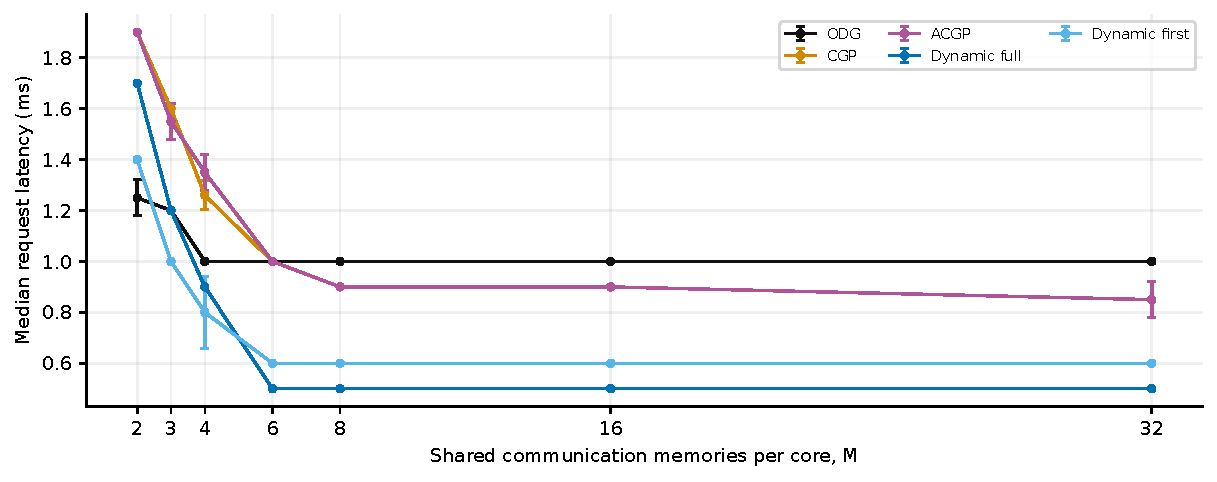
\includegraphics[width=.94\linewidth,height=.255\textheight,keepaspectratio]{figures/memory/mesh_xy_request_latency_median_ms.pdf}\captionof{figure}{Run-level mean and sample SD. Shared trace aliases are counted once.}\end{center}
\begin{center}{\scriptsize\setlength{\tabcolsep}{3pt}
\begin{tabular}{lrrrrr}
\toprule
M & ODG & CGP & ACGP & Dynamic full & Dynamic first \\
\midrule
2 & $1.250\pm0.071$ & $1.900\pm0.000$ & $1.900\pm0.000$ & $1.700\pm0.000$ & $1.400\pm0.000$ \\
3 & $1.200\pm0.000$ & $1.600\pm0.000$ & $1.550\pm0.071$ & $1.200\pm0.000$ & $1.000\pm0.000$ \\
4 & $1.000\pm0.000$ & $1.260\pm0.056$ & $1.350\pm0.071$ & $0.9000\pm0.0000$ & $0.8000\pm0.1414$ \\
6 & $1.000\pm0.000$ & $1.000\pm0.000$ & $1.000\pm0.000$ & $0.5000\pm0.0000$ & $0.6000\pm0.0000$ \\
8 & $1.000\pm0.000$ & $0.9000\pm0.0000$ & $0.9000\pm0.0000$ & $0.5000\pm0.0000$ & $0.6000\pm0.0000$ \\
16 & $1.000\pm0.000$ & $0.9000\pm0.0000$ & $0.9000\pm0.0000$ & $0.5000\pm0.0000$ & $0.6000\pm0.0000$ \\
32 & $1.000\pm0.000$ & $0.8500\pm0.0707$ & $0.8500\pm0.0707$ & $0.5000\pm0.0000$ & $0.6000\pm0.0000$ \\
\bottomrule\end{tabular}}
\captionof{table}{Mean $\pm$ sample SD; n/a denotes a metric outside that policy's instrumentation.}
{\footnotesize\href{https://github.com/sanjeevkrishnaa/Compiler-Driven-ACE/blob/codex/ace-scheduler-correctness/docs/latex/qft96_final/data/memory_mesh_xy_request_latency_median_ms.csv}{Exact CSV values and sample counts}}
\end{center}
\clearpage
\subsection*{p95 request latency}
\begin{center}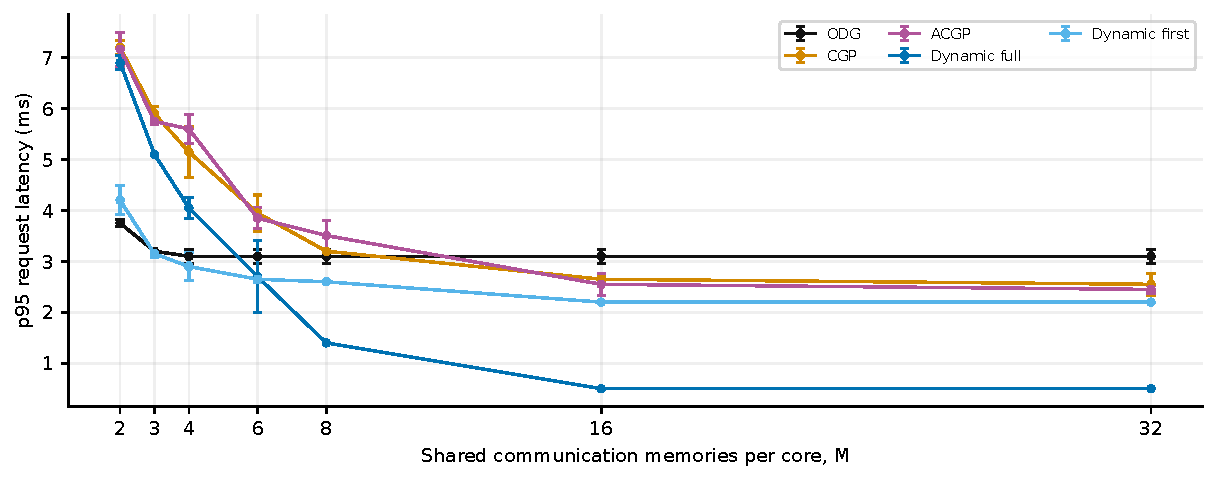
\includegraphics[width=.94\linewidth,height=.255\textheight,keepaspectratio]{figures/memory/mesh_xy_request_latency_p95_ms.pdf}\captionof{figure}{Run-level mean and sample SD. Shared trace aliases are counted once.}\end{center}
\begin{center}{\scriptsize\setlength{\tabcolsep}{3pt}
\begin{tabular}{lrrrrr}
\toprule
M & ODG & CGP & ACGP & Dynamic full & Dynamic first \\
\midrule
2 & $3.750\pm0.071$ & $7.200\pm0.141$ & $7.166\pm0.332$ & $6.900\pm0.141$ & $4.200\pm0.283$ \\
3 & $3.200\pm0.000$ & $5.900\pm0.141$ & $5.750\pm0.071$ & $5.100\pm0.000$ & $3.150\pm0.071$ \\
4 & $3.100\pm0.141$ & $5.150\pm0.495$ & $5.600\pm0.283$ & $4.050\pm0.212$ & $2.900\pm0.283$ \\
6 & $3.100\pm0.141$ & $3.950\pm0.354$ & $3.850\pm0.212$ & $2.700\pm0.707$ & $2.650\pm0.071$ \\
8 & $3.100\pm0.141$ & $3.200\pm0.000$ & $3.508\pm0.294$ & $1.400\pm0.000$ & $2.600\pm0.000$ \\
16 & $3.100\pm0.141$ & $2.650\pm0.071$ & $2.550\pm0.212$ & $0.5000\pm0.0000$ & $2.200\pm0.000$ \\
32 & $3.100\pm0.141$ & $2.550\pm0.212$ & $2.450\pm0.071$ & $0.5000\pm0.0000$ & $2.200\pm0.000$ \\
\bottomrule\end{tabular}}
\captionof{table}{Mean $\pm$ sample SD; n/a denotes a metric outside that policy's instrumentation.}
{\footnotesize\href{https://github.com/sanjeevkrishnaa/Compiler-Driven-ACE/blob/codex/ace-scheduler-correctness/docs/latex/qft96_final/data/memory_mesh_xy_request_latency_p95_ms.csv}{Exact CSV values and sample counts}}
\end{center}
\subsection*{Maximum request latency}
\begin{center}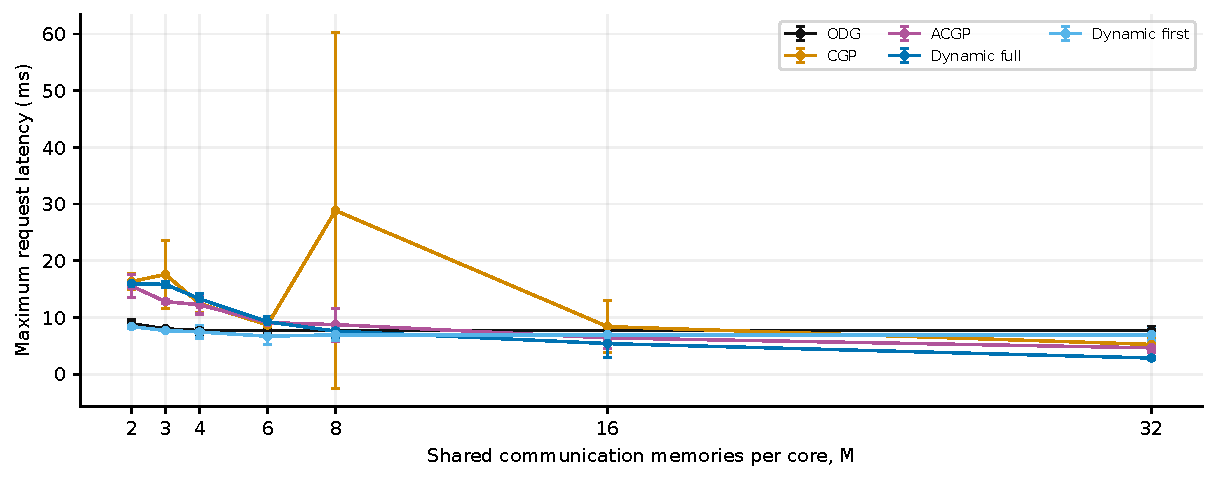
\includegraphics[width=.94\linewidth,height=.255\textheight,keepaspectratio]{figures/memory/mesh_xy_request_latency_max_ms.pdf}\captionof{figure}{Run-level mean and sample SD. Shared trace aliases are counted once.}\end{center}
\begin{center}{\scriptsize\setlength{\tabcolsep}{3pt}
\begin{tabular}{lrrrrr}
\toprule
M & ODG & CGP & ACGP & Dynamic full & Dynamic first \\
\midrule
2 & $8.900\pm0.707$ & $16.350\pm1.485$ & $15.550\pm2.051$ & $15.950\pm0.354$ & $8.400\pm0.283$ \\
3 & $8.000\pm0.283$ & $17.591\pm5.953$ & $12.800\pm0.283$ & $15.850\pm0.495$ & $7.700\pm0.000$ \\
4 & $7.700\pm0.707$ & $12.468\pm1.651$ & $12.250\pm1.626$ & $13.300\pm0.990$ & $7.450\pm1.061$ \\
6 & $7.700\pm0.707$ & $8.700\pm0.990$ & $9.100\pm0.283$ & $9.250\pm0.919$ & $6.700\pm1.414$ \\
8 & $7.700\pm0.707$ & $28.871\pm31.437$ & $8.750\pm2.899$ & $7.600\pm1.273$ & $6.950\pm1.061$ \\
16 & $7.700\pm0.707$ & $8.400\pm4.526$ & $6.400\pm1.839$ & $5.400\pm2.404$ & $6.950\pm1.061$ \\
32 & $7.700\pm0.707$ & $5.250\pm1.061$ & $4.650\pm0.778$ & $2.850\pm0.212$ & $6.950\pm1.061$ \\
\bottomrule\end{tabular}}
\captionof{table}{Mean $\pm$ sample SD; n/a denotes a metric outside that policy's instrumentation.}
{\footnotesize\href{https://github.com/sanjeevkrishnaa/Compiler-Driven-ACE/blob/codex/ace-scheduler-correctness/docs/latex/qft96_final/data/memory_mesh_xy_request_latency_max_ms.csv}{Exact CSV values and sample counts}}
\end{center}
\clearpage
\subsection*{Communication makespan}
\begin{center}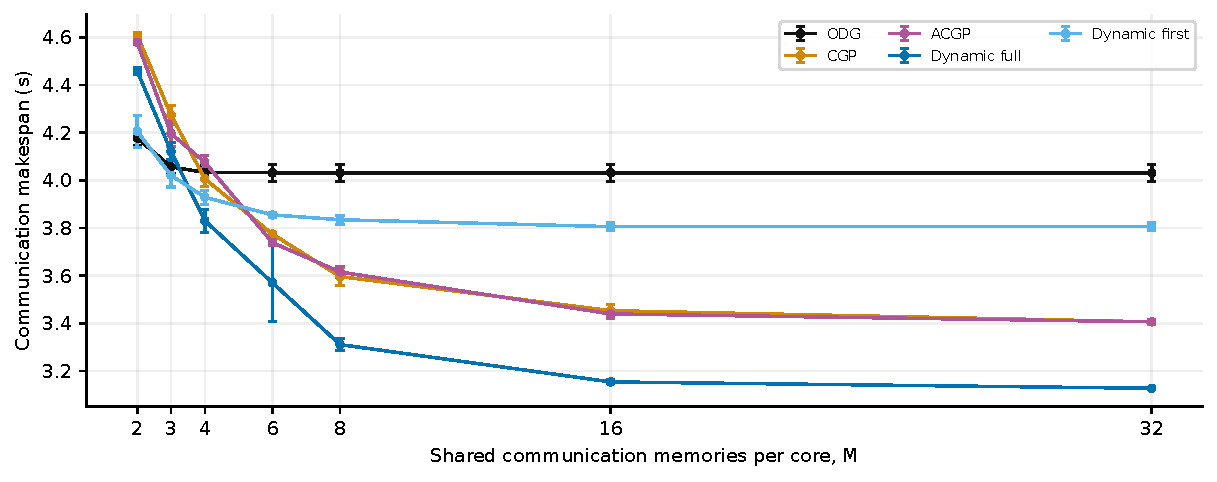
\includegraphics[width=.94\linewidth,height=.255\textheight,keepaspectratio]{figures/memory/mesh_xy_end_to_end_latency_ms.pdf}\captionof{figure}{Run-level mean and sample SD. Shared trace aliases are counted once.}\end{center}
\begin{center}{\scriptsize\setlength{\tabcolsep}{3pt}
\begin{tabular}{lrrrrr}
\toprule
M & ODG & CGP & ACGP & Dynamic full & Dynamic first \\
\midrule
2 & $4.177\pm0.031$ & $4.608\pm0.012$ & $4.578\pm0.008$ & $4.458\pm0.014$ & $4.205\pm0.067$ \\
3 & $4.056\pm0.026$ & $4.273\pm0.041$ & $4.196\pm0.054$ & $4.121\pm0.036$ & $4.021\pm0.049$ \\
4 & $4.033\pm0.031$ & $4.006\pm0.031$ & $4.075\pm0.028$ & $3.830\pm0.048$ & $3.928\pm0.029$ \\
6 & $4.031\pm0.036$ & $3.774\pm0.004$ & $3.738\pm0.013$ & $3.570\pm0.163$ & $3.854\pm0.009$ \\
8 & $4.031\pm0.036$ & $3.596\pm0.039$ & $3.615\pm0.022$ & $3.311\pm0.024$ & $3.834\pm0.019$ \\
16 & $4.031\pm0.036$ & $3.453\pm0.024$ & $3.439\pm0.018$ & $3.154\pm0.008$ & $3.805\pm0.015$ \\
32 & $4.031\pm0.036$ & $3.406\pm0.009$ & $3.406\pm0.008$ & $3.127\pm0.002$ & $3.805\pm0.015$ \\
\bottomrule\end{tabular}}
\captionof{table}{Mean $\pm$ sample SD; n/a denotes a metric outside that policy's instrumentation.}
{\footnotesize\href{https://github.com/sanjeevkrishnaa/Compiler-Driven-ACE/blob/codex/ace-scheduler-correctness/docs/latex/qft96_final/data/memory_mesh_xy_end_to_end_latency_ms.csv}{Exact CSV values and sample counts}}
\end{center}
\subsection*{Mean admission wait}
\begin{center}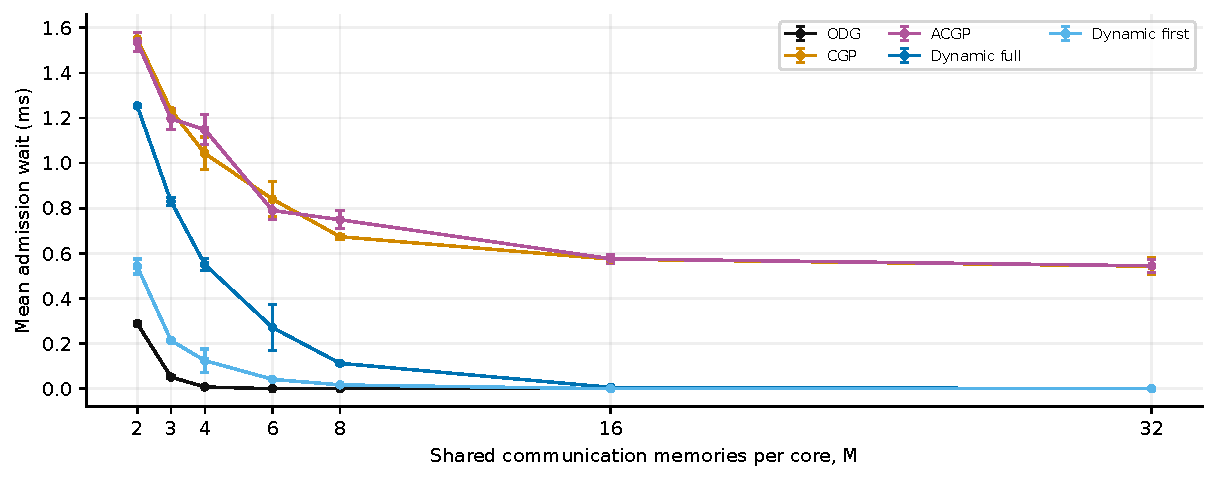
\includegraphics[width=.94\linewidth,height=.255\textheight,keepaspectratio]{figures/memory/mesh_xy_average_admission_wait_ms.pdf}\captionof{figure}{Run-level mean and sample SD. Shared trace aliases are counted once.}\end{center}
\begin{center}{\scriptsize\setlength{\tabcolsep}{3pt}
\begin{tabular}{lrrrrr}
\toprule
M & ODG & CGP & ACGP & Dynamic full & Dynamic first \\
\midrule
2 & $0.2891\pm0.0096$ & $1.550\pm0.004$ & $1.538\pm0.041$ & $1.254\pm0.005$ & $0.5419\pm0.0332$ \\
3 & $0.0517\pm0.0057$ & $1.234\pm0.003$ & $1.197\pm0.045$ & $0.8302\pm0.0184$ & $0.2138\pm0.0034$ \\
4 & $0.0080\pm0.0022$ & $1.043\pm0.073$ & $1.149\pm0.067$ & $0.5507\pm0.0249$ & $0.1248\pm0.0514$ \\
6 & $0.0000\pm0.0000$ & $0.8403\pm0.0779$ & $0.7902\pm0.0415$ & $0.2715\pm0.1027$ & $0.0418\pm0.0052$ \\
8 & $0.0000\pm0.0000$ & $0.6739\pm0.0106$ & $0.7492\pm0.0396$ & $0.1128\pm0.0036$ & $0.0171\pm0.0013$ \\
16 & $0.0000\pm0.0000$ & $0.5746\pm0.0055$ & $0.5761\pm0.0197$ & $0.0062\pm0.0002$ & $0.0000\pm0.0000$ \\
32 & $0.0000\pm0.0000$ & $0.5431\pm0.0371$ & $0.5449\pm0.0279$ & $0.0000\pm0.0000$ & $0.0000\pm0.0000$ \\
\bottomrule\end{tabular}}
\captionof{table}{Mean $\pm$ sample SD; n/a denotes a metric outside that policy's instrumentation.}
{\footnotesize\href{https://github.com/sanjeevkrishnaa/Compiler-Driven-ACE/blob/codex/ace-scheduler-correctness/docs/latex/qft96_final/data/memory_mesh_xy_average_admission_wait_ms.csv}{Exact CSV values and sample counts}}
\end{center}
\clearpage
\subsection*{Delivered EPR fidelity}
\begin{center}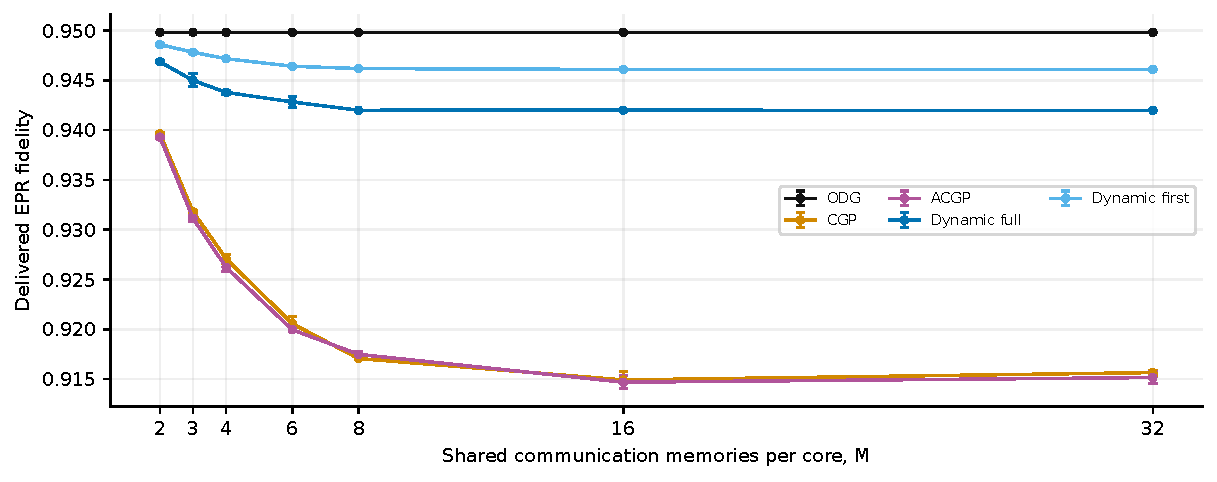
\includegraphics[width=.94\linewidth,height=.255\textheight,keepaspectratio]{figures/memory/mesh_xy_average_delivered_epr_fidelity.pdf}\captionof{figure}{Run-level mean and sample SD. Shared trace aliases are counted once.}\end{center}
\begin{center}{\scriptsize\setlength{\tabcolsep}{3pt}
\begin{tabular}{lrrrrr}
\toprule
M & ODG & CGP & ACGP & Dynamic full & Dynamic first \\
\midrule
2 & $0.9498\pm0.0000$ & $0.9396\pm0.0002$ & $0.9393\pm0.0002$ & $0.9469\pm0.0001$ & $0.9486\pm0.0001$ \\
3 & $0.9498\pm0.0000$ & $0.9318\pm0.0001$ & $0.9311\pm0.0003$ & $0.9450\pm0.0007$ & $0.9478\pm0.0001$ \\
4 & $0.9498\pm0.0000$ & $0.9271\pm0.0004$ & $0.9262\pm0.0004$ & $0.9438\pm0.0002$ & $0.9472\pm0.0000$ \\
6 & $0.9498\pm0.0000$ & $0.9206\pm0.0007$ & $0.9200\pm0.0001$ & $0.9428\pm0.0006$ & $0.9464\pm0.0000$ \\
8 & $0.9498\pm0.0000$ & $0.9171\pm0.0001$ & $0.9175\pm0.0003$ & $0.9420\pm0.0000$ & $0.9462\pm0.0000$ \\
16 & $0.9498\pm0.0000$ & $0.9149\pm0.0009$ & $0.9147\pm0.0007$ & $0.9420\pm0.0000$ & $0.9461\pm0.0000$ \\
32 & $0.9498\pm0.0000$ & $0.9157\pm0.0002$ & $0.9152\pm0.0006$ & $0.9420\pm0.0000$ & $0.9461\pm0.0000$ \\
\bottomrule\end{tabular}}
\captionof{table}{Mean $\pm$ sample SD; n/a denotes a metric outside that policy's instrumentation.}
{\footnotesize\href{https://github.com/sanjeevkrishnaa/Compiler-Driven-ACE/blob/codex/ace-scheduler-correctness/docs/latex/qft96_final/data/memory_mesh_xy_average_delivered_epr_fidelity.csv}{Exact CSV values and sample counts}}
\end{center}
\subsection*{Compiler readiness fraction}
\begin{center}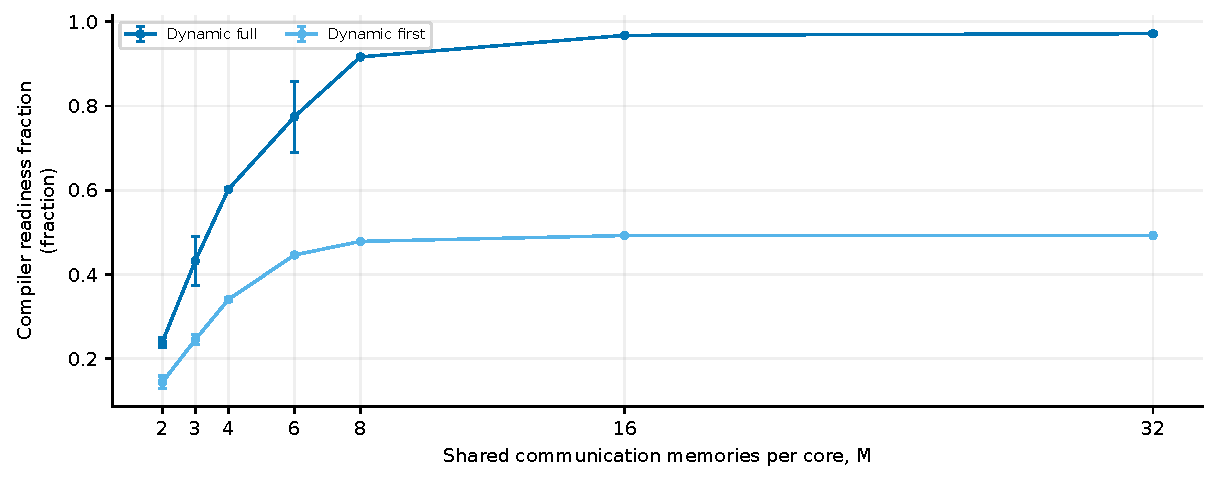
\includegraphics[width=.94\linewidth,height=.255\textheight,keepaspectratio]{figures/memory/mesh_xy_pregenerated_success_rate.pdf}\captionof{figure}{Run-level mean and sample SD. Shared trace aliases are counted once.}\end{center}
\begin{center}{\scriptsize\setlength{\tabcolsep}{3pt}
\begin{tabular}{lrrrrr}
\toprule
M & ODG & CGP & ACGP & Dynamic full & Dynamic first \\
\midrule
2 & n/a & n/a & n/a & $0.2390\pm0.0111$ & $0.1438\pm0.0151$ \\
3 & n/a & n/a & n/a & $0.4321\pm0.0580$ & $0.2451\pm0.0120$ \\
4 & n/a & n/a & n/a & $0.6017\pm0.0007$ & $0.3403\pm0.0044$ \\
6 & n/a & n/a & n/a & $0.7740\pm0.0836$ & $0.4462\pm0.0042$ \\
8 & n/a & n/a & n/a & $0.9163\pm0.0013$ & $0.4785\pm0.0005$ \\
16 & n/a & n/a & n/a & $0.9675\pm0.0004$ & $0.4924\pm0.0009$ \\
32 & n/a & n/a & n/a & $0.9715\pm0.0020$ & $0.4924\pm0.0009$ \\
\bottomrule\end{tabular}}
\captionof{table}{Mean $\pm$ sample SD; n/a denotes a metric outside that policy's instrumentation.}
{\footnotesize\href{https://github.com/sanjeevkrishnaa/Compiler-Driven-ACE/blob/codex/ace-scheduler-correctness/docs/latex/qft96_final/data/memory_mesh_xy_pregenerated_success_rate.csv}{Exact CSV values and sample counts}}
\end{center}
\clearpage
\subsection*{Intended compiler-hit fraction}
\begin{center}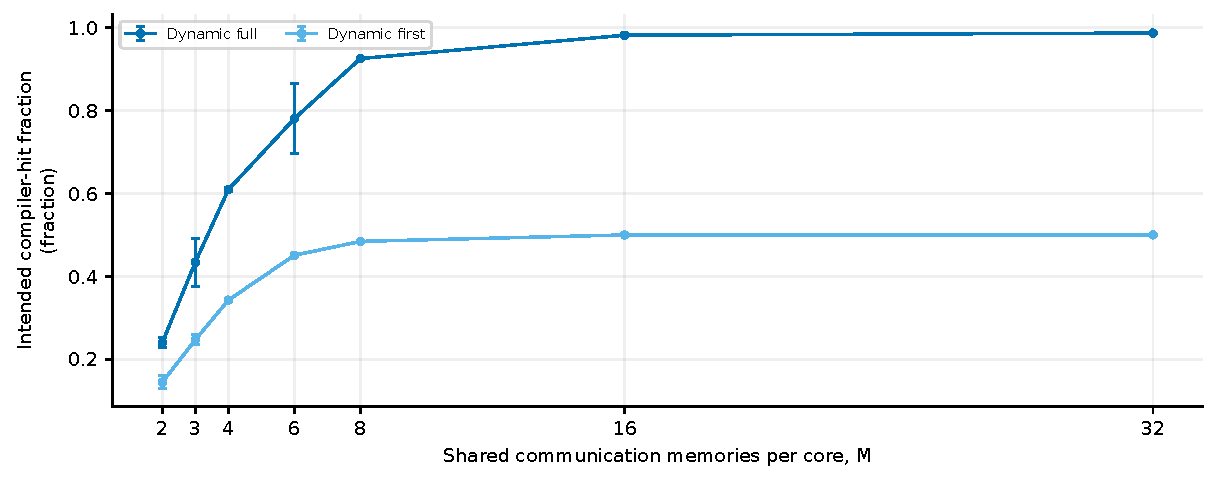
\includegraphics[width=.94\linewidth,height=.255\textheight,keepaspectratio]{figures/memory/mesh_xy_intended_request_hit_rate.pdf}\captionof{figure}{Run-level mean and sample SD. Shared trace aliases are counted once.}\end{center}
\begin{center}{\scriptsize\setlength{\tabcolsep}{3pt}
\begin{tabular}{lrrrrr}
\toprule
M & ODG & CGP & ACGP & Dynamic full & Dynamic first \\
\midrule
2 & n/a & n/a & n/a & $0.2402\pm0.0120$ & $0.1446\pm0.0155$ \\
3 & n/a & n/a & n/a & $0.4342\pm0.0584$ & $0.2472\pm0.0120$ \\
4 & n/a & n/a & n/a & $0.6094\pm0.0044$ & $0.3429\pm0.0033$ \\
6 & n/a & n/a & n/a & $0.7808\pm0.0848$ & $0.4511\pm0.0038$ \\
8 & n/a & n/a & n/a & $0.9258\pm0.0016$ & $0.4846\pm0.0002$ \\
16 & n/a & n/a & n/a & $0.9822\pm0.0033$ & $0.5003\pm0.0004$ \\
32 & n/a & n/a & n/a & $0.9875\pm0.0016$ & $0.5003\pm0.0004$ \\
\bottomrule\end{tabular}}
\captionof{table}{Mean $\pm$ sample SD; n/a denotes a metric outside that policy's instrumentation.}
{\footnotesize\href{https://github.com/sanjeevkrishnaa/Compiler-Driven-ACE/blob/codex/ace-scheduler-correctness/docs/latex/qft96_final/data/memory_mesh_xy_intended_request_hit_rate.csv}{Exact CSV values and sample counts}}
\end{center}
\subsection*{Compiler fallback fraction}
\begin{center}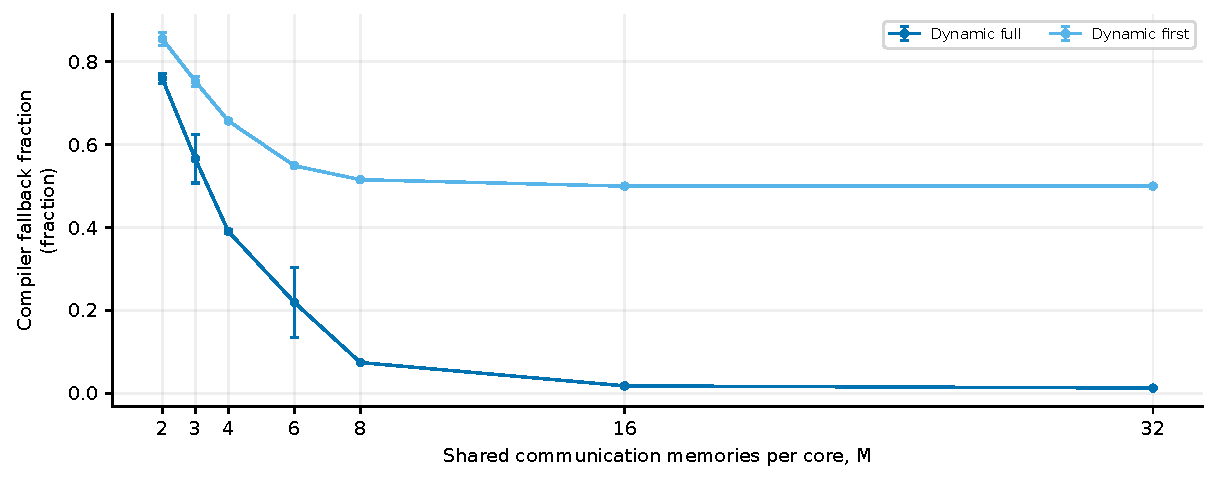
\includegraphics[width=.94\linewidth,height=.255\textheight,keepaspectratio]{figures/memory/mesh_xy_on_demand_fallback_rate.pdf}\captionof{figure}{Run-level mean and sample SD. Shared trace aliases are counted once.}\end{center}
\begin{center}{\scriptsize\setlength{\tabcolsep}{3pt}
\begin{tabular}{lrrrrr}
\toprule
M & ODG & CGP & ACGP & Dynamic full & Dynamic first \\
\midrule
2 & n/a & n/a & n/a & $0.7598\pm0.0120$ & $0.8554\pm0.0155$ \\
3 & n/a & n/a & n/a & $0.5658\pm0.0584$ & $0.7528\pm0.0120$ \\
4 & n/a & n/a & n/a & $0.3906\pm0.0044$ & $0.6571\pm0.0033$ \\
6 & n/a & n/a & n/a & $0.2192\pm0.0848$ & $0.5489\pm0.0038$ \\
8 & n/a & n/a & n/a & $0.0742\pm0.0016$ & $0.5154\pm0.0002$ \\
16 & n/a & n/a & n/a & $0.0178\pm0.0033$ & $0.4997\pm0.0004$ \\
32 & n/a & n/a & n/a & $0.0125\pm0.0016$ & $0.4997\pm0.0004$ \\
\bottomrule\end{tabular}}
\captionof{table}{Mean $\pm$ sample SD; n/a denotes a metric outside that policy's instrumentation.}
{\footnotesize\href{https://github.com/sanjeevkrishnaa/Compiler-Driven-ACE/blob/codex/ace-scheduler-correctness/docs/latex/qft96_final/data/memory_mesh_xy_on_demand_fallback_rate.csv}{Exact CSV values and sample counts}}
\end{center}
\clearpage
\subsection*{Compiler-cache waste}
\begin{center}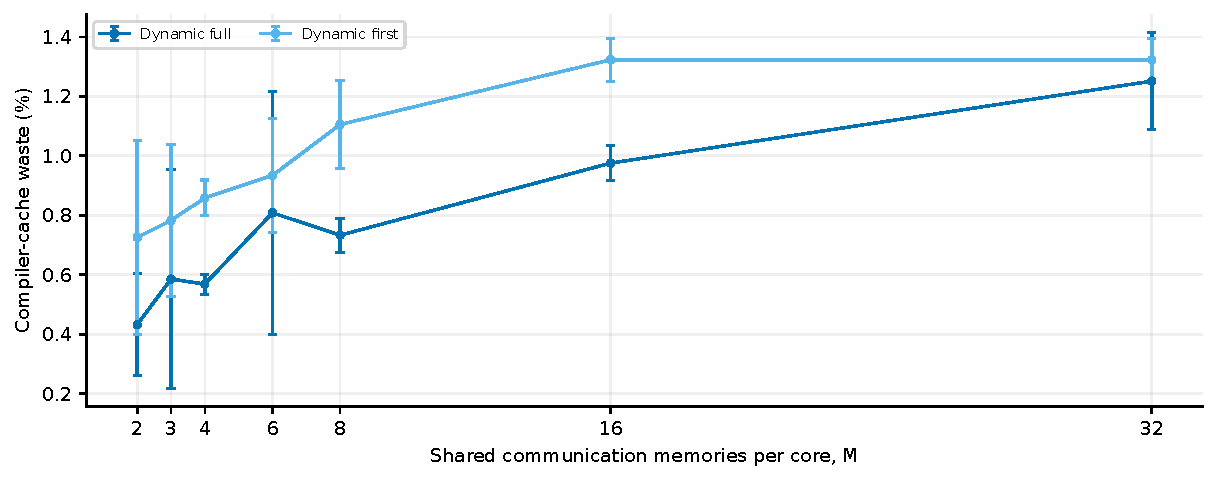
\includegraphics[width=.94\linewidth,height=.255\textheight,keepaspectratio]{figures/memory/mesh_xy_compiler_waste_percentage.pdf}\captionof{figure}{Run-level mean and sample SD. Shared trace aliases are counted once.}\end{center}
\begin{center}{\scriptsize\setlength{\tabcolsep}{3pt}
\begin{tabular}{lrrrrr}
\toprule
M & ODG & CGP & ACGP & Dynamic full & Dynamic first \\
\midrule
2 & n/a & n/a & n/a & $0.4320\pm0.1722$ & $0.7255\pm0.3260$ \\
3 & n/a & n/a & n/a & $0.5854\pm0.3690$ & $0.7827\pm0.2558$ \\
4 & n/a & n/a & n/a & $0.5684\pm0.0337$ & $0.8582\pm0.0604$ \\
6 & n/a & n/a & n/a & $0.8081\pm0.4090$ & $0.9339\pm0.1906$ \\
8 & n/a & n/a & n/a & $0.7330\pm0.0570$ & $1.105\pm0.147$ \\
16 & n/a & n/a & n/a & $0.9755\pm0.0579$ & $1.323\pm0.072$ \\
32 & n/a & n/a & n/a & $1.251\pm0.164$ & $1.323\pm0.072$ \\
\bottomrule\end{tabular}}
\captionof{table}{Mean $\pm$ sample SD; n/a denotes a metric outside that policy's instrumentation.}
{\footnotesize\href{https://github.com/sanjeevkrishnaa/Compiler-Driven-ACE/blob/codex/ace-scheduler-correctness/docs/latex/qft96_final/data/memory_mesh_xy_compiler_waste_percentage.csv}{Exact CSV values and sample counts}}
\end{center}
\subsection*{Native-protocol waste}
\begin{center}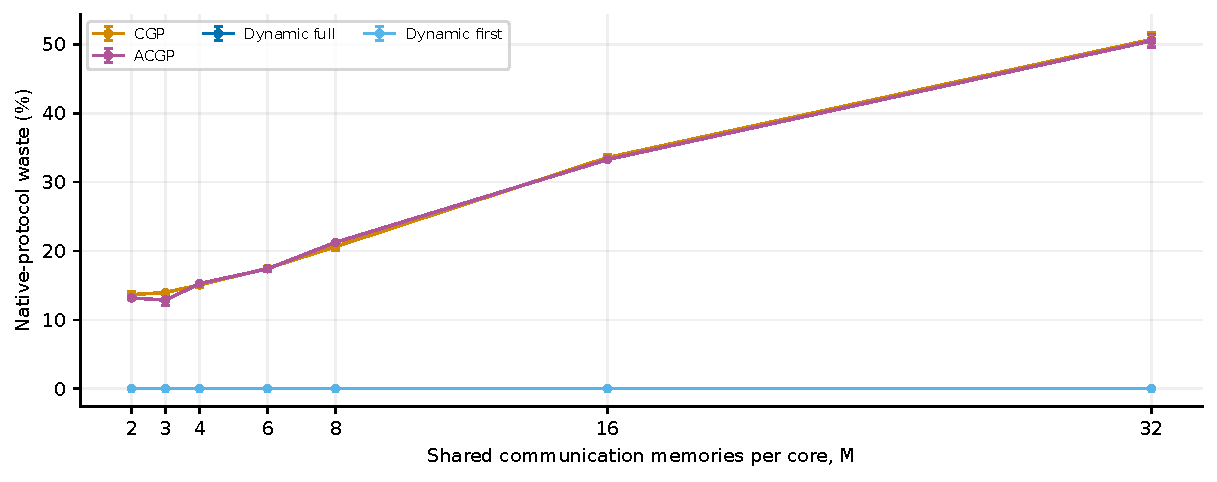
\includegraphics[width=.94\linewidth,height=.255\textheight,keepaspectratio]{figures/memory/mesh_xy_protocol_waste_percentage.pdf}\captionof{figure}{Run-level mean and sample SD. Shared trace aliases are counted once.}\end{center}
\begin{center}{\scriptsize\setlength{\tabcolsep}{3pt}
\begin{tabular}{lrrrrr}
\toprule
M & ODG & CGP & ACGP & Dynamic full & Dynamic first \\
\midrule
2 & n/a & $13.658\pm0.398$ & $13.185\pm0.195$ & $0.0000\pm0.0000$ & $0.0000\pm0.0000$ \\
3 & n/a & $13.974\pm0.073$ & $12.865\pm0.778$ & $0.0000\pm0.0000$ & $0.0000\pm0.0000$ \\
4 & n/a & $15.065\pm0.392$ & $15.269\pm0.209$ & $0.0000\pm0.0000$ & $0.0000\pm0.0000$ \\
6 & n/a & $17.490\pm0.122$ & $17.405\pm0.394$ & $0.0000\pm0.0000$ & $0.0000\pm0.0000$ \\
8 & n/a & $20.622\pm0.599$ & $21.252\pm0.082$ & $0.0000\pm0.0000$ & $0.0000\pm0.0000$ \\
16 & n/a & $33.559\pm0.465$ & $33.265\pm0.024$ & $0.0000\pm0.0000$ & $0.0000\pm0.0000$ \\
32 & n/a & $50.705\pm1.032$ & $50.498\pm0.959$ & $0.0000\pm0.0000$ & $0.0000\pm0.0000$ \\
\bottomrule\end{tabular}}
\captionof{table}{Mean $\pm$ sample SD; n/a denotes a metric outside that policy's instrumentation.}
{\footnotesize\href{https://github.com/sanjeevkrishnaa/Compiler-Driven-ACE/blob/codex/ace-scheduler-correctness/docs/latex/qft96_final/data/memory_mesh_xy_protocol_waste_percentage.csv}{Exact CSV values and sample counts}}
\end{center}
\clearpage
\subsection*{Compiler-pair expiry}
\begin{center}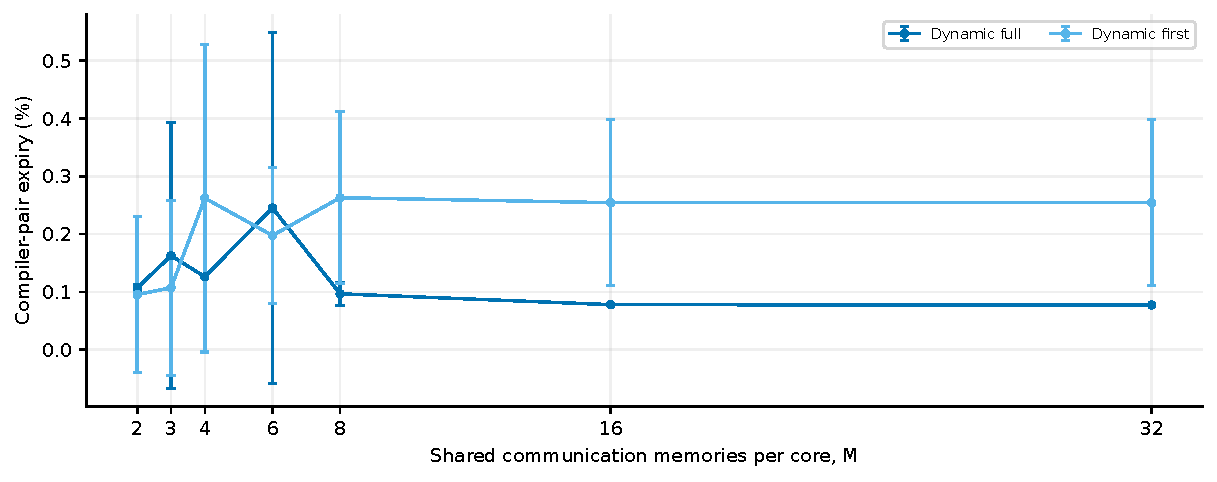
\includegraphics[width=.94\linewidth,height=.255\textheight,keepaspectratio]{figures/memory/mesh_xy_compiler_expiry_percentage.pdf}\captionof{figure}{Run-level mean and sample SD. Shared trace aliases are counted once.}\end{center}
\begin{center}{\scriptsize\setlength{\tabcolsep}{3pt}
\begin{tabular}{lrrrrr}
\toprule
M & ODG & CGP & ACGP & Dynamic full & Dynamic first \\
\midrule
2 & n/a & n/a & n/a & $0.1071\pm0.0052$ & $0.0956\pm0.1352$ \\
3 & n/a & n/a & n/a & $0.1628\pm0.2302$ & $0.1071\pm0.1514$ \\
4 & n/a & n/a & n/a & $0.1263\pm0.0009$ & $0.2623\pm0.2661$ \\
6 & n/a & n/a & n/a & $0.2454\pm0.3038$ & $0.1977\pm0.1181$ \\
8 & n/a & n/a & n/a & $0.0968\pm0.0198$ & $0.2631\pm0.1484$ \\
16 & n/a & n/a & n/a & $0.0780\pm0.0002$ & $0.2545\pm0.1439$ \\
32 & n/a & n/a & n/a & $0.0774\pm0.0000$ & $0.2545\pm0.1439$ \\
\bottomrule\end{tabular}}
\captionof{table}{Mean $\pm$ sample SD; n/a denotes a metric outside that policy's instrumentation.}
{\footnotesize\href{https://github.com/sanjeevkrishnaa/Compiler-Driven-ACE/blob/codex/ace-scheduler-correctness/docs/latex/qft96_final/data/memory_mesh_xy_compiler_expiry_percentage.csv}{Exact CSV values and sample counts}}
\end{center}
\subsection*{Used compiler-pair storage time}
\begin{center}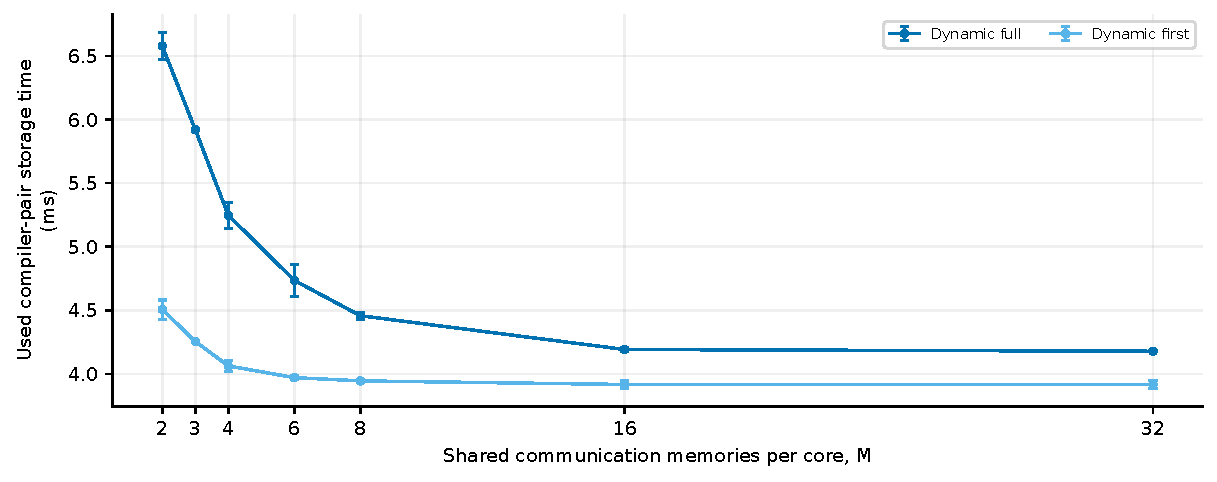
\includegraphics[width=.94\linewidth,height=.255\textheight,keepaspectratio]{figures/memory/mesh_xy_average_storage_time_ms.pdf}\captionof{figure}{Run-level mean and sample SD. Shared trace aliases are counted once.}\end{center}
\begin{center}{\scriptsize\setlength{\tabcolsep}{3pt}
\begin{tabular}{lrrrrr}
\toprule
M & ODG & CGP & ACGP & Dynamic full & Dynamic first \\
\midrule
2 & n/a & n/a & n/a & $6.578\pm0.107$ & $4.506\pm0.075$ \\
3 & n/a & n/a & n/a & $5.921\pm0.001$ & $4.256\pm0.009$ \\
4 & n/a & n/a & n/a & $5.247\pm0.103$ & $4.063\pm0.041$ \\
6 & n/a & n/a & n/a & $4.735\pm0.124$ & $3.971\pm0.014$ \\
8 & n/a & n/a & n/a & $4.458\pm0.026$ & $3.945\pm0.014$ \\
16 & n/a & n/a & n/a & $4.192\pm0.014$ & $3.917\pm0.034$ \\
32 & n/a & n/a & n/a & $4.178\pm0.003$ & $3.917\pm0.034$ \\
\bottomrule\end{tabular}}
\captionof{table}{Mean $\pm$ sample SD; n/a denotes a metric outside that policy's instrumentation.}
{\footnotesize\href{https://github.com/sanjeevkrishnaa/Compiler-Driven-ACE/blob/codex/ace-scheduler-correctness/docs/latex/qft96_final/data/memory_mesh_xy_average_storage_time_ms.csv}{Exact CSV values and sample counts}}
\end{center}
\clearpage
\subsection*{Delivered-hop throughput}
\begin{center}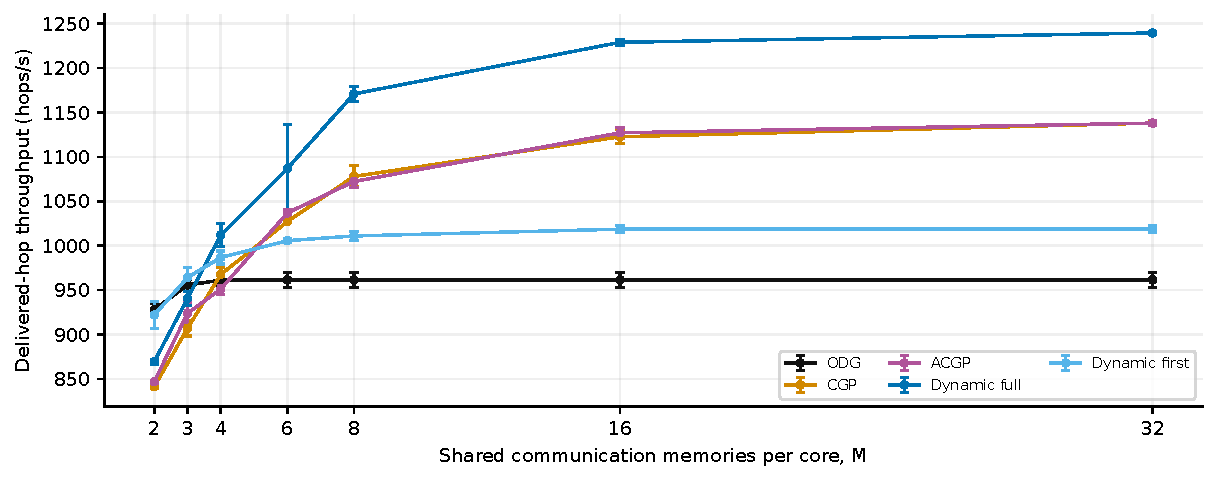
\includegraphics[width=.94\linewidth,height=.255\textheight,keepaspectratio]{figures/memory/mesh_xy_hop_throughput_s.pdf}\captionof{figure}{Run-level mean and sample SD. Shared trace aliases are counted once.}\end{center}
\begin{center}{\scriptsize\setlength{\tabcolsep}{3pt}
\begin{tabular}{lrrrrr}
\toprule
M & ODG & CGP & ACGP & Dynamic full & Dynamic first \\
\midrule
2 & $927.92\pm6.83$ & $841.10\pm2.21$ & $846.68\pm1.42$ & $869.42\pm2.63$ & $921.98\pm14.73$ \\
3 & $955.68\pm6.13$ & $907.05\pm8.75$ & $923.90\pm11.97$ & $940.66\pm8.18$ & $964.11\pm11.75$ \\
4 & $961.17\pm7.33$ & $967.59\pm7.40$ & $951.16\pm6.47$ & $1012.03\pm12.59$ & $986.67\pm7.33$ \\
6 & $961.53\pm8.53$ & $1027.05\pm1.16$ & $1036.88\pm3.65$ & $1086.92\pm49.67$ & $1005.60\pm2.32$ \\
8 & $961.53\pm8.53$ & $1077.97\pm11.78$ & $1072.23\pm6.43$ & $1170.85\pm8.65$ & $1010.92\pm5.05$ \\
16 & $961.53\pm8.53$ & $1122.61\pm7.82$ & $1127.05\pm5.86$ & $1228.94\pm3.22$ & $1018.59\pm4.07$ \\
32 & $961.53\pm8.53$ & $1138.05\pm2.96$ & $1138.00\pm2.53$ & $1239.49\pm0.73$ & $1018.59\pm4.07$ \\
\bottomrule\end{tabular}}
\captionof{table}{Mean $\pm$ sample SD; n/a denotes a metric outside that policy's instrumentation.}
{\footnotesize\href{https://github.com/sanjeevkrishnaa/Compiler-Driven-ACE/blob/codex/ace-scheduler-correctness/docs/latex/qft96_final/data/memory_mesh_xy_hop_throughput_s.csv}{Exact CSV values and sample counts}}
\end{center}
\subsection*{Completion fraction}
\begin{center}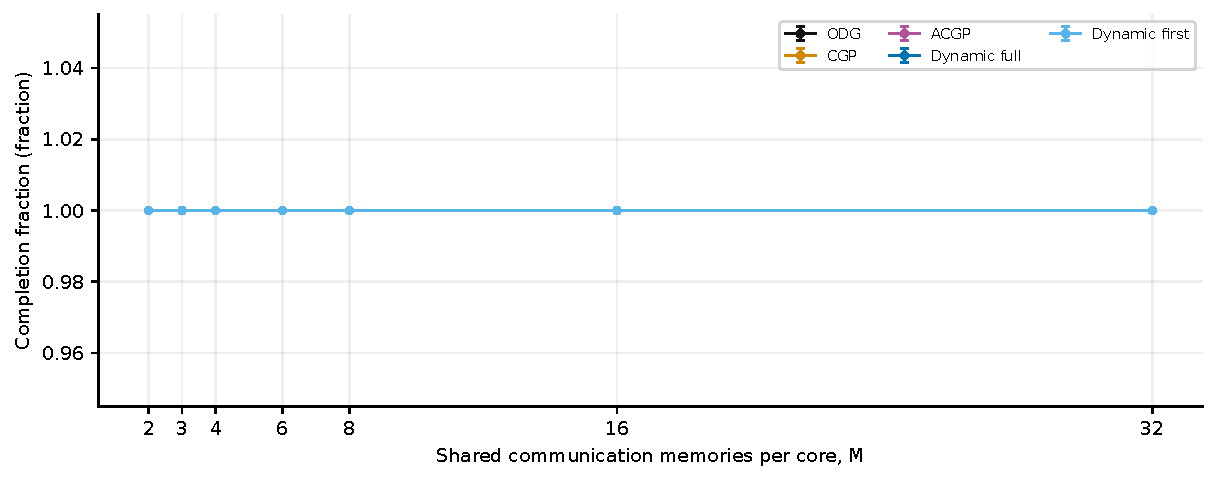
\includegraphics[width=.94\linewidth,height=.255\textheight,keepaspectratio]{figures/memory/mesh_xy_completion_rate.pdf}\captionof{figure}{Run-level mean and sample SD. Shared trace aliases are counted once.}\end{center}
\begin{center}{\scriptsize\setlength{\tabcolsep}{3pt}
\begin{tabular}{lrrrrr}
\toprule
M & ODG & CGP & ACGP & Dynamic full & Dynamic first \\
\midrule
2 & $1.000\pm0.000$ & $1.000\pm0.000$ & $1.000\pm0.000$ & $1.000\pm0.000$ & $1.000\pm0.000$ \\
3 & $1.000\pm0.000$ & $1.000\pm0.000$ & $1.000\pm0.000$ & $1.000\pm0.000$ & $1.000\pm0.000$ \\
4 & $1.000\pm0.000$ & $1.000\pm0.000$ & $1.000\pm0.000$ & $1.000\pm0.000$ & $1.000\pm0.000$ \\
6 & $1.000\pm0.000$ & $1.000\pm0.000$ & $1.000\pm0.000$ & $1.000\pm0.000$ & $1.000\pm0.000$ \\
8 & $1.000\pm0.000$ & $1.000\pm0.000$ & $1.000\pm0.000$ & $1.000\pm0.000$ & $1.000\pm0.000$ \\
16 & $1.000\pm0.000$ & $1.000\pm0.000$ & $1.000\pm0.000$ & $1.000\pm0.000$ & $1.000\pm0.000$ \\
32 & $1.000\pm0.000$ & $1.000\pm0.000$ & $1.000\pm0.000$ & $1.000\pm0.000$ & $1.000\pm0.000$ \\
\bottomrule\end{tabular}}
\captionof{table}{Mean $\pm$ sample SD; n/a denotes a metric outside that policy's instrumentation.}
{\footnotesize\href{https://github.com/sanjeevkrishnaa/Compiler-Driven-ACE/blob/codex/ace-scheduler-correctness/docs/latex/qft96_final/data/memory_mesh_xy_completion_rate.csv}{Exact CSV values and sample counts}}
\end{center}
\clearpage
\subsection*{Maximum admission wait}
\begin{center}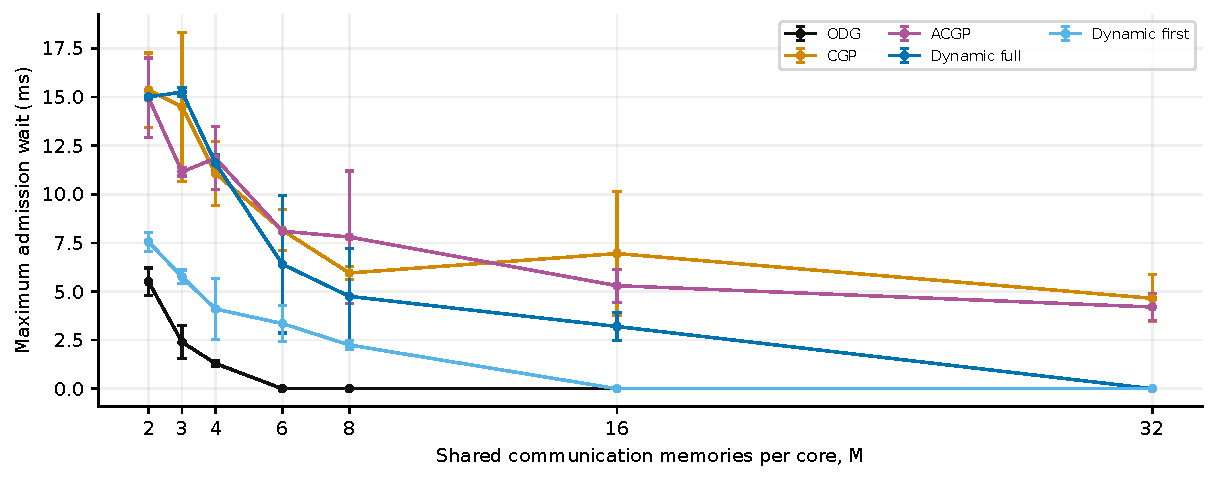
\includegraphics[width=.94\linewidth,height=.255\textheight,keepaspectratio]{figures/memory/mesh_xy_max_admission_wait_ms.pdf}\captionof{figure}{Run-level mean and sample SD. Shared trace aliases are counted once.}\end{center}
\begin{center}{\scriptsize\setlength{\tabcolsep}{3pt}
\begin{tabular}{lrrrrr}
\toprule
M & ODG & CGP & ACGP & Dynamic full & Dynamic first \\
\midrule
2 & $5.500\pm0.707$ & $15.350\pm1.909$ & $14.950\pm2.051$ & $15.000\pm0.000$ & $7.550\pm0.495$ \\
3 & $2.400\pm0.849$ & $14.491\pm3.832$ & $11.150\pm0.212$ & $15.250\pm0.212$ & $5.750\pm0.354$ \\
4 & $1.300\pm0.141$ & $11.067\pm1.651$ & $11.850\pm1.626$ & $11.600\pm0.424$ & $4.100\pm1.556$ \\
6 & $0.0000\pm0.0000$ & $8.150\pm1.061$ & $8.100\pm0.000$ & $6.400\pm3.536$ & $3.350\pm0.919$ \\
8 & $0.0000\pm0.0000$ & $5.950\pm0.354$ & $7.800\pm3.394$ & $4.750\pm2.475$ & $2.250\pm0.212$ \\
16 & $0.0000\pm0.0000$ & $6.950\pm3.182$ & $5.300\pm0.849$ & $3.200\pm0.707$ & $0.0000\pm0.0000$ \\
32 & $0.0000\pm0.0000$ & $4.650\pm1.202$ & $4.200\pm0.707$ & $0.0000\pm0.0000$ & $0.0000\pm0.0000$ \\
\bottomrule\end{tabular}}
\captionof{table}{Mean $\pm$ sample SD; n/a denotes a metric outside that policy's instrumentation.}
{\footnotesize\href{https://github.com/sanjeevkrishnaa/Compiler-Driven-ACE/blob/codex/ace-scheduler-correctness/docs/latex/qft96_final/data/memory_mesh_xy_max_admission_wait_ms.csv}{Exact CSV values and sample counts}}
\end{center}
\subsection*{Requests with admission wait}
\begin{center}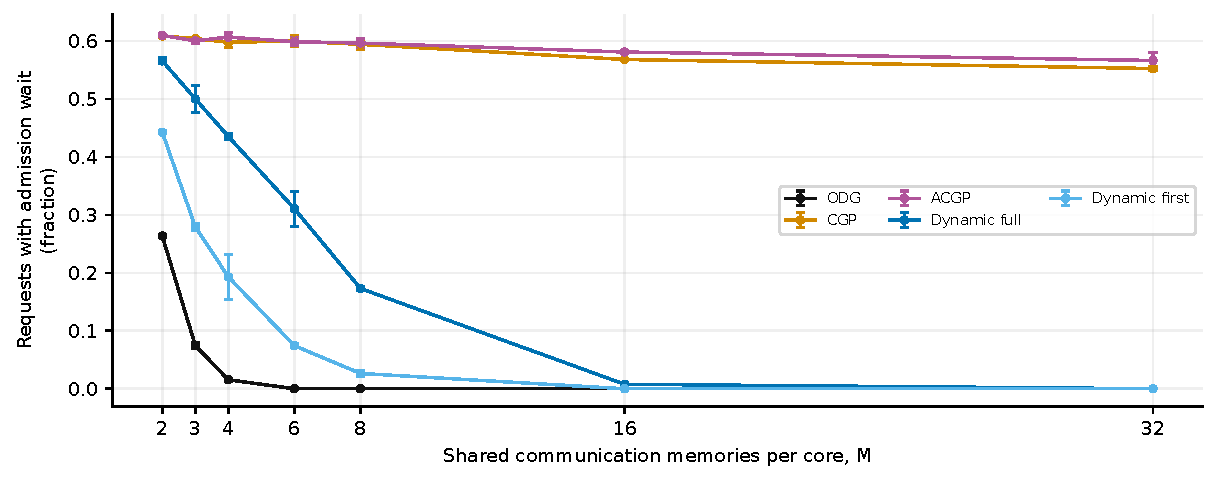
\includegraphics[width=.94\linewidth,height=.255\textheight,keepaspectratio]{figures/memory/mesh_xy_requests_that_waited_fraction.pdf}\captionof{figure}{Run-level mean and sample SD. Shared trace aliases are counted once.}\end{center}
\begin{center}{\scriptsize\setlength{\tabcolsep}{3pt}
\begin{tabular}{lrrrrr}
\toprule
M & ODG & CGP & ACGP & Dynamic full & Dynamic first \\
\midrule
2 & $0.2637\pm0.0033$ & $0.6089\pm0.0007$ & $0.6099\pm0.0022$ & $0.5659\pm0.0053$ & $0.4427\pm0.0022$ \\
3 & $0.0746\pm0.0047$ & $0.6044\pm0.0013$ & $0.6005\pm0.0053$ & $0.5003\pm0.0230$ & $0.2795\pm0.0064$ \\
4 & $0.0155\pm0.0029$ & $0.5980\pm0.0095$ & $0.6069\pm0.0082$ & $0.4354\pm0.0049$ & $0.1931\pm0.0385$ \\
6 & $0.0000\pm0.0000$ & $0.6000\pm0.0100$ & $0.5989\pm0.0071$ & $0.3108\pm0.0301$ & $0.0743\pm0.0033$ \\
8 & $0.0000\pm0.0000$ & $0.5944\pm0.0080$ & $0.5966\pm0.0075$ & $0.1731\pm0.0036$ & $0.0264\pm0.0046$ \\
16 & $0.0000\pm0.0000$ & $0.5682\pm0.0005$ & $0.5811\pm0.0013$ & $0.0077\pm0.0015$ & $0.0000\pm0.0000$ \\
32 & $0.0000\pm0.0000$ & $0.5526\pm0.0036$ & $0.5666\pm0.0135$ & $0.0000\pm0.0000$ & $0.0000\pm0.0000$ \\
\bottomrule\end{tabular}}
\captionof{table}{Mean $\pm$ sample SD; n/a denotes a metric outside that policy's instrumentation.}
{\footnotesize\href{https://github.com/sanjeevkrishnaa/Compiler-Driven-ACE/blob/codex/ace-scheduler-correctness/docs/latex/qft96_final/data/memory_mesh_xy_requests_that_waited_fraction.csv}{Exact CSV values and sample counts}}
\end{center}
\clearpage
\subsection*{Recorded reservation-setup counter}
\begin{center}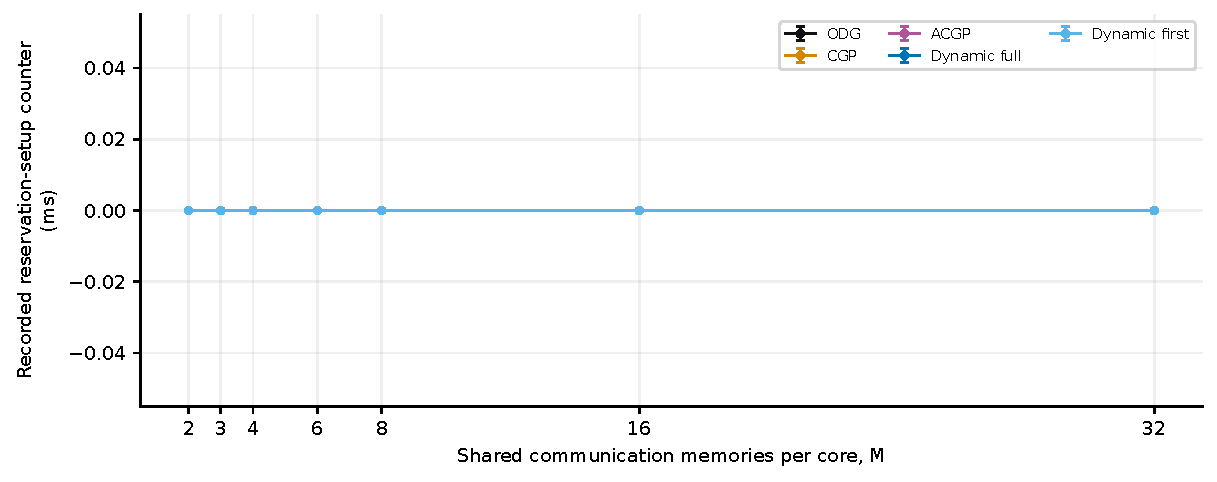
\includegraphics[width=.94\linewidth,height=.255\textheight,keepaspectratio]{figures/memory/mesh_xy_avg_reservation_setup_time_ms.pdf}\captionof{figure}{Run-level mean and sample SD. Shared trace aliases are counted once.}\end{center}
\begin{center}{\scriptsize\setlength{\tabcolsep}{3pt}
\begin{tabular}{lrrrrr}
\toprule
M & ODG & CGP & ACGP & Dynamic full & Dynamic first \\
\midrule
2 & $0.0000\pm0.0000$ & $0.0000\pm0.0000$ & $0.0000\pm0.0000$ & $0.0000\pm0.0000$ & $0.0000\pm0.0000$ \\
3 & $0.0000\pm0.0000$ & $0.0000\pm0.0000$ & $0.0000\pm0.0000$ & $0.0000\pm0.0000$ & $0.0000\pm0.0000$ \\
4 & $0.0000\pm0.0000$ & $0.0000\pm0.0000$ & $0.0000\pm0.0000$ & $0.0000\pm0.0000$ & $0.0000\pm0.0000$ \\
6 & $0.0000\pm0.0000$ & $0.0000\pm0.0000$ & $0.0000\pm0.0000$ & $0.0000\pm0.0000$ & $0.0000\pm0.0000$ \\
8 & $0.0000\pm0.0000$ & $0.0000\pm0.0000$ & $0.0000\pm0.0000$ & $0.0000\pm0.0000$ & $0.0000\pm0.0000$ \\
16 & $0.0000\pm0.0000$ & $0.0000\pm0.0000$ & $0.0000\pm0.0000$ & $0.0000\pm0.0000$ & $0.0000\pm0.0000$ \\
32 & $0.0000\pm0.0000$ & $0.0000\pm0.0000$ & $0.0000\pm0.0000$ & $0.0000\pm0.0000$ & $0.0000\pm0.0000$ \\
\bottomrule\end{tabular}}
\captionof{table}{Mean $\pm$ sample SD; n/a denotes a metric outside that policy's instrumentation.}
{\footnotesize\href{https://github.com/sanjeevkrishnaa/Compiler-Driven-ACE/blob/codex/ace-scheduler-correctness/docs/latex/qft96_final/data/memory_mesh_xy_avg_reservation_setup_time_ms.csv}{Exact CSV values and sample counts}}
\end{center}
\subsection*{Mean generation/service time}
\begin{center}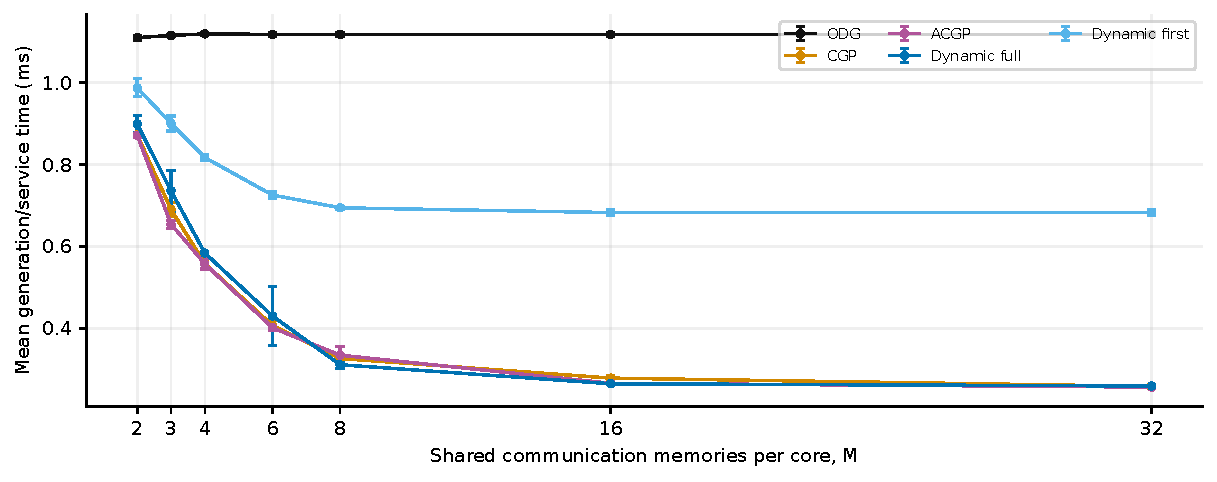
\includegraphics[width=.94\linewidth,height=.255\textheight,keepaspectratio]{figures/memory/mesh_xy_avg_entanglement_generation_time_ms.pdf}\captionof{figure}{Run-level mean and sample SD. Shared trace aliases are counted once.}\end{center}
\begin{center}{\scriptsize\setlength{\tabcolsep}{3pt}
\begin{tabular}{lrrrrr}
\toprule
M & ODG & CGP & ACGP & Dynamic full & Dynamic first \\
\midrule
2 & $1.110\pm0.006$ & $0.8724\pm0.0038$ & $0.8709\pm0.0047$ & $0.8989\pm0.0212$ & $0.9872\pm0.0219$ \\
3 & $1.115\pm0.003$ & $0.6898\pm0.0181$ & $0.6541\pm0.0098$ & $0.7355\pm0.0504$ & $0.9000\pm0.0183$ \\
4 & $1.119\pm0.004$ & $0.5576\pm0.0023$ & $0.5571\pm0.0126$ & $0.5836\pm0.0046$ & $0.8167\pm0.0071$ \\
6 & $1.117\pm0.004$ & $0.4067\pm0.0117$ & $0.4009\pm0.0077$ & $0.4297\pm0.0714$ & $0.7252\pm0.0077$ \\
8 & $1.117\pm0.004$ & $0.3261\pm0.0043$ & $0.3341\pm0.0222$ & $0.3108\pm0.0082$ & $0.6940\pm0.0039$ \\
16 & $1.117\pm0.004$ & $0.2780\pm0.0059$ & $0.2654\pm0.0039$ & $0.2643\pm0.0018$ & $0.6823\pm0.0078$ \\
32 & $1.117\pm0.004$ & $0.2577\pm0.0057$ & $0.2561\pm0.0004$ & $0.2587\pm0.0006$ & $0.6823\pm0.0078$ \\
\bottomrule\end{tabular}}
\captionof{table}{Mean $\pm$ sample SD; n/a denotes a metric outside that policy's instrumentation.}
{\footnotesize\href{https://github.com/sanjeevkrishnaa/Compiler-Driven-ACE/blob/codex/ace-scheduler-correctness/docs/latex/qft96_final/data/memory_mesh_xy_avg_entanglement_generation_time_ms.csv}{Exact CSV values and sample counts}}
\end{center}
\clearpage
\subsection*{Recorded retry-wait time}
\begin{center}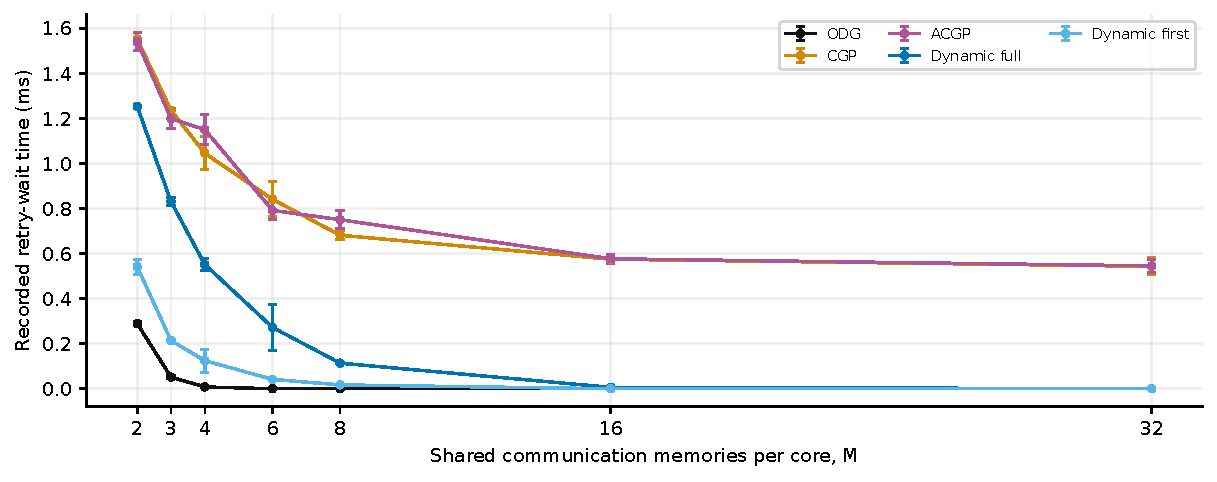
\includegraphics[width=.94\linewidth,height=.255\textheight,keepaspectratio]{figures/memory/mesh_xy_avg_retry_wait_time_ms.pdf}\captionof{figure}{Run-level mean and sample SD. Shared trace aliases are counted once.}\end{center}
\begin{center}{\scriptsize\setlength{\tabcolsep}{3pt}
\begin{tabular}{lrrrrr}
\toprule
M & ODG & CGP & ACGP & Dynamic full & Dynamic first \\
\midrule
2 & $0.2891\pm0.0096$ & $1.552\pm0.004$ & $1.541\pm0.041$ & $1.254\pm0.005$ & $0.5419\pm0.0332$ \\
3 & $0.0517\pm0.0057$ & $1.236\pm0.002$ & $1.200\pm0.044$ & $0.8305\pm0.0186$ & $0.2138\pm0.0034$ \\
4 & $0.0080\pm0.0022$ & $1.045\pm0.073$ & $1.151\pm0.066$ & $0.5515\pm0.0248$ & $0.1248\pm0.0514$ \\
6 & $0.0000\pm0.0000$ & $0.8413\pm0.0774$ & $0.7919\pm0.0409$ & $0.2724\pm0.1025$ & $0.0418\pm0.0052$ \\
8 & $0.0000\pm0.0000$ & $0.6815\pm0.0193$ & $0.7503\pm0.0395$ & $0.1137\pm0.0024$ & $0.0171\pm0.0013$ \\
16 & $0.0000\pm0.0000$ & $0.5749\pm0.0055$ & $0.5770\pm0.0191$ & $0.0062\pm0.0002$ & $0.0000\pm0.0000$ \\
32 & $0.0000\pm0.0000$ & $0.5433\pm0.0373$ & $0.5454\pm0.0282$ & $0.0000\pm0.0000$ & $0.0000\pm0.0000$ \\
\bottomrule\end{tabular}}
\captionof{table}{Mean $\pm$ sample SD; n/a denotes a metric outside that policy's instrumentation.}
{\footnotesize\href{https://github.com/sanjeevkrishnaa/Compiler-Driven-ACE/blob/codex/ace-scheduler-correctness/docs/latex/qft96_final/data/memory_mesh_xy_avg_retry_wait_time_ms.csv}{Exact CSV values and sample counts}}
\end{center}
\subsection*{Request retries}
\begin{center}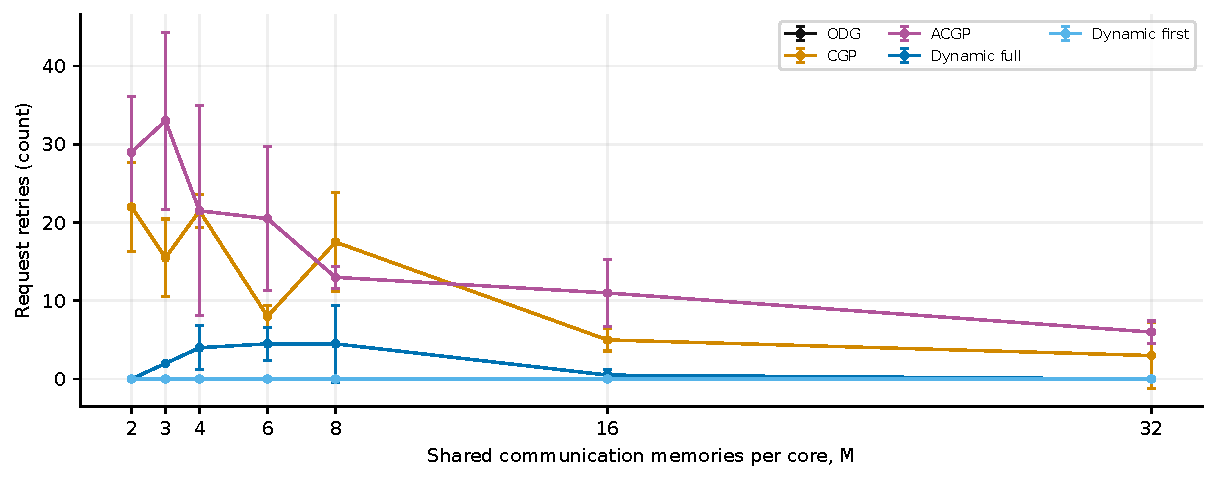
\includegraphics[width=.94\linewidth,height=.255\textheight,keepaspectratio]{figures/memory/mesh_xy_total_retries.pdf}\captionof{figure}{Run-level mean and sample SD. Shared trace aliases are counted once.}\end{center}
\begin{center}{\scriptsize\setlength{\tabcolsep}{3pt}
\begin{tabular}{lrrrrr}
\toprule
M & ODG & CGP & ACGP & Dynamic full & Dynamic first \\
\midrule
2 & $0.0000\pm0.0000$ & $22.000\pm5.657$ & $29.000\pm7.071$ & $0.0000\pm0.0000$ & $0.0000\pm0.0000$ \\
3 & $0.0000\pm0.0000$ & $15.500\pm4.950$ & $33.000\pm11.314$ & $2.000\pm0.000$ & $0.0000\pm0.0000$ \\
4 & $0.0000\pm0.0000$ & $21.500\pm2.121$ & $21.500\pm13.435$ & $4.000\pm2.828$ & $0.0000\pm0.0000$ \\
6 & $0.0000\pm0.0000$ & $8.000\pm1.414$ & $20.500\pm9.192$ & $4.500\pm2.121$ & $0.0000\pm0.0000$ \\
8 & $0.0000\pm0.0000$ & $17.500\pm6.364$ & $13.000\pm1.414$ & $4.500\pm4.950$ & $0.0000\pm0.0000$ \\
16 & $0.0000\pm0.0000$ & $5.000\pm1.414$ & $11.000\pm4.243$ & $0.5000\pm0.7071$ & $0.0000\pm0.0000$ \\
32 & $0.0000\pm0.0000$ & $3.000\pm4.243$ & $6.000\pm1.414$ & $0.0000\pm0.0000$ & $0.0000\pm0.0000$ \\
\bottomrule\end{tabular}}
\captionof{table}{Mean $\pm$ sample SD; n/a denotes a metric outside that policy's instrumentation.}
{\footnotesize\href{https://github.com/sanjeevkrishnaa/Compiler-Driven-ACE/blob/codex/ace-scheduler-correctness/docs/latex/qft96_final/data/memory_mesh_xy_total_retries.csv}{Exact CSV values and sample counts}}
\end{center}
\clearpage
\subsection*{Requests with retries}
\begin{center}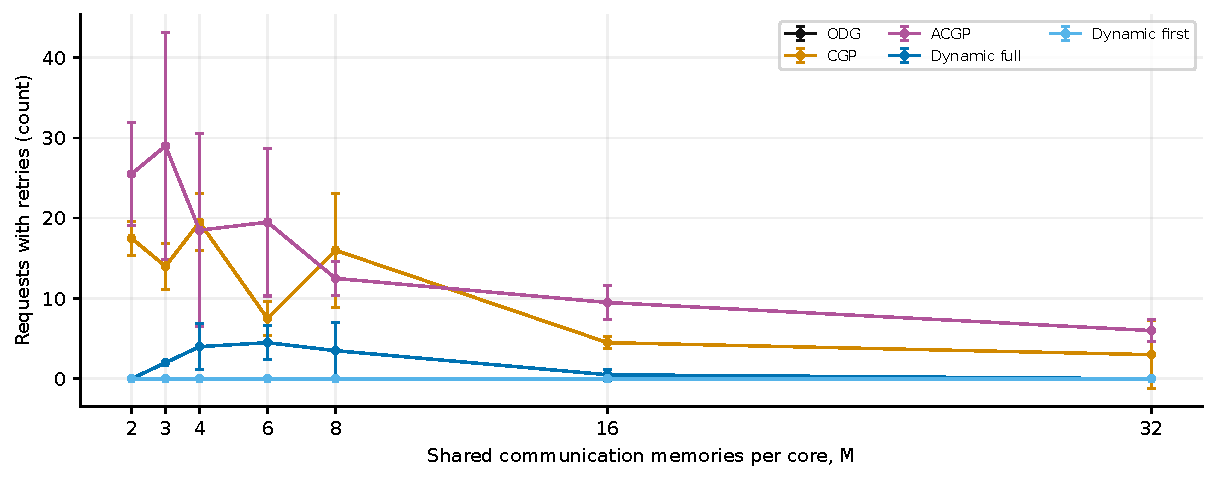
\includegraphics[width=.94\linewidth,height=.255\textheight,keepaspectratio]{figures/memory/mesh_xy_requests_with_retries.pdf}\captionof{figure}{Run-level mean and sample SD. Shared trace aliases are counted once.}\end{center}
\begin{center}{\scriptsize\setlength{\tabcolsep}{3pt}
\begin{tabular}{lrrrrr}
\toprule
M & ODG & CGP & ACGP & Dynamic full & Dynamic first \\
\midrule
2 & $0.0000\pm0.0000$ & $17.500\pm2.121$ & $25.500\pm6.364$ & $0.0000\pm0.0000$ & $0.0000\pm0.0000$ \\
3 & $0.0000\pm0.0000$ & $14.000\pm2.828$ & $29.000\pm14.142$ & $2.000\pm0.000$ & $0.0000\pm0.0000$ \\
4 & $0.0000\pm0.0000$ & $19.500\pm3.536$ & $18.500\pm12.021$ & $4.000\pm2.828$ & $0.0000\pm0.0000$ \\
6 & $0.0000\pm0.0000$ & $7.500\pm2.121$ & $19.500\pm9.192$ & $4.500\pm2.121$ & $0.0000\pm0.0000$ \\
8 & $0.0000\pm0.0000$ & $16.000\pm7.071$ & $12.500\pm2.121$ & $3.500\pm3.536$ & $0.0000\pm0.0000$ \\
16 & $0.0000\pm0.0000$ & $4.500\pm0.707$ & $9.500\pm2.121$ & $0.5000\pm0.7071$ & $0.0000\pm0.0000$ \\
32 & $0.0000\pm0.0000$ & $3.000\pm4.243$ & $6.000\pm1.414$ & $0.0000\pm0.0000$ & $0.0000\pm0.0000$ \\
\bottomrule\end{tabular}}
\captionof{table}{Mean $\pm$ sample SD; n/a denotes a metric outside that policy's instrumentation.}
{\footnotesize\href{https://github.com/sanjeevkrishnaa/Compiler-Driven-ACE/blob/codex/ace-scheduler-correctness/docs/latex/qft96_final/data/memory_mesh_xy_requests_with_retries.csv}{Exact CSV values and sample counts}}
\end{center}
\subsection*{Native-protocol generated-pair counter}
\begin{center}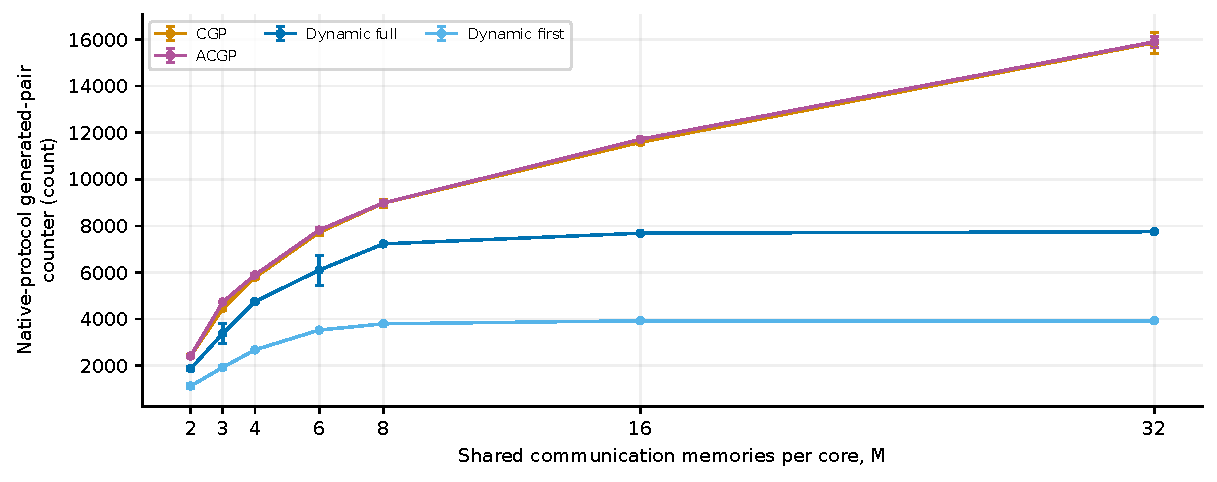
\includegraphics[width=.94\linewidth,height=.255\textheight,keepaspectratio]{figures/memory/mesh_xy_protocol_generated_pairs.pdf}\captionof{figure}{Run-level mean and sample SD. Shared trace aliases are counted once.}\end{center}
\begin{center}{\scriptsize\setlength{\tabcolsep}{3pt}
\begin{tabular}{lrrrrr}
\toprule
M & ODG & CGP & ACGP & Dynamic full & Dynamic first \\
\midrule
2 & n/a & $2424.00\pm39.60$ & $2420.00\pm67.88$ & $1870.00\pm90.51$ & $1129.00\pm117.38$ \\
3 & n/a & $4458.00\pm67.88$ & $4734.00\pm11.31$ & $3385.00\pm442.65$ & $1931.00\pm89.10$ \\
4 & n/a & $5794.00\pm65.05$ & $5895.00\pm80.61$ & $4751.00\pm32.53$ & $2681.00\pm24.04$ \\
6 & n/a & $7725.00\pm142.84$ & $7821.00\pm120.21$ & $6101.00\pm637.81$ & $3530.00\pm36.77$ \\
8 & n/a & $8983.00\pm171.12$ & $8987.00\pm111.72$ & $7230.00\pm16.97$ & $3799.00\pm7.07$ \\
16 & n/a & $11592.00\pm76.37$ & $11718.00\pm84.85$ & $7689.00\pm21.21$ & $3930.00\pm0.00$ \\
32 & n/a & $15865.00\pm445.48$ & $15902.00\pm243.24$ & $7752.00\pm0.00$ & $3930.00\pm0.00$ \\
\bottomrule\end{tabular}}
\captionof{table}{Mean $\pm$ sample SD; n/a denotes a metric outside that policy's instrumentation.}
{\footnotesize\href{https://github.com/sanjeevkrishnaa/Compiler-Driven-ACE/blob/codex/ace-scheduler-correctness/docs/latex/qft96_final/data/memory_mesh_xy_protocol_generated_pairs.csv}{Exact CSV values and sample counts}}
\end{center}
\clearpage
\subsection*{Native-protocol used-pair counter}
\begin{center}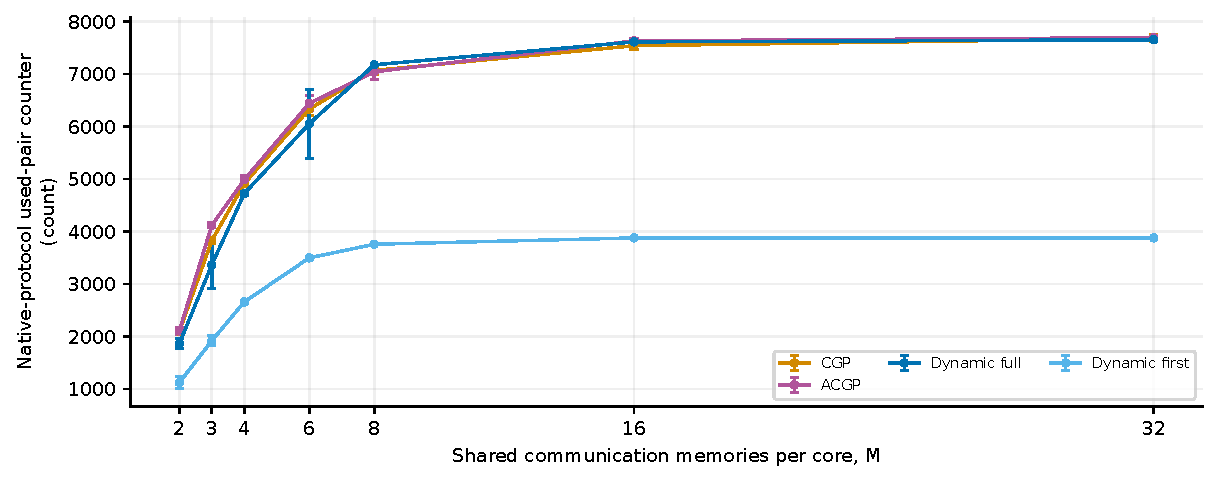
\includegraphics[width=.94\linewidth,height=.255\textheight,keepaspectratio]{figures/memory/mesh_xy_protocol_used_pairs.pdf}\captionof{figure}{Run-level mean and sample SD. Shared trace aliases are counted once.}\end{center}
\begin{center}{\scriptsize\setlength{\tabcolsep}{3pt}
\begin{tabular}{lrrrrr}
\toprule
M & ODG & CGP & ACGP & Dynamic full & Dynamic first \\
\midrule
2 & n/a & $2094.00\pm36.77$ & $2106.00\pm59.40$ & $1862.00\pm93.34$ & $1121.00\pm120.21$ \\
3 & n/a & $3827.00\pm63.64$ & $4117.00\pm46.67$ & $3366.00\pm452.55$ & $1916.00\pm93.34$ \\
4 & n/a & $4911.00\pm18.38$ & $4986.00\pm82.02$ & $4724.00\pm33.94$ & $2658.00\pm25.46$ \\
6 & n/a & $6335.00\pm128.69$ & $6442.00\pm141.42$ & $6053.00\pm657.61$ & $3497.00\pm29.70$ \\
8 & n/a & $7070.00\pm67.88$ & $7044.00\pm147.08$ & $7177.00\pm12.73$ & $3757.00\pm1.41$ \\
16 & n/a & $7541.00\pm69.30$ & $7632.00\pm48.08$ & $7614.00\pm25.46$ & $3878.00\pm2.83$ \\
32 & n/a & $7684.00\pm65.05$ & $7696.00\pm16.97$ & $7655.00\pm12.73$ & $3878.00\pm2.83$ \\
\bottomrule\end{tabular}}
\captionof{table}{Mean $\pm$ sample SD; n/a denotes a metric outside that policy's instrumentation.}
{\footnotesize\href{https://github.com/sanjeevkrishnaa/Compiler-Driven-ACE/blob/codex/ace-scheduler-correctness/docs/latex/qft96_final/data/memory_mesh_xy_protocol_used_pairs.csv}{Exact CSV values and sample counts}}
\end{center}
\subsection*{Native-protocol unused-pair counter}
\begin{center}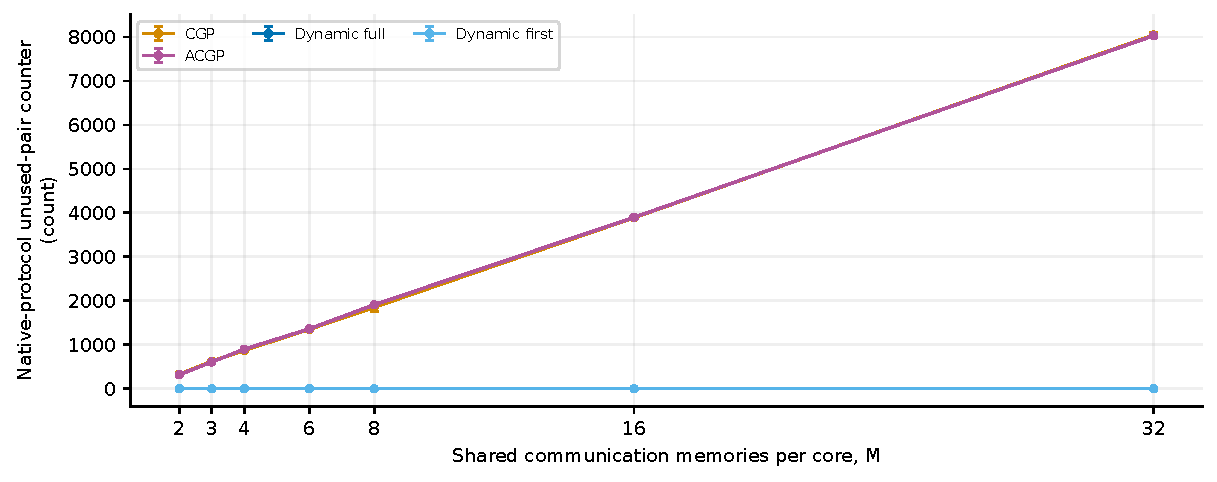
\includegraphics[width=.94\linewidth,height=.255\textheight,keepaspectratio]{figures/memory/mesh_xy_protocol_unused_pairs.pdf}\captionof{figure}{Run-level mean and sample SD. Shared trace aliases are counted once.}\end{center}
\begin{center}{\scriptsize\setlength{\tabcolsep}{3pt}
\begin{tabular}{lrrrrr}
\toprule
M & ODG & CGP & ACGP & Dynamic full & Dynamic first \\
\midrule
2 & n/a & $331.00\pm4.24$ & $319.00\pm4.24$ & $0.0000\pm0.0000$ & $0.0000\pm0.0000$ \\
3 & n/a & $623.00\pm12.73$ & $609.00\pm35.36$ & $0.0000\pm0.0000$ & $0.0000\pm0.0000$ \\
4 & n/a & $873.00\pm32.53$ & $900.00\pm0.00$ & $0.0000\pm0.0000$ & $0.0000\pm0.0000$ \\
6 & n/a & $1351.00\pm15.56$ & $1361.00\pm9.90$ & $0.0000\pm0.0000$ & $0.0000\pm0.0000$ \\
8 & n/a & $1853.00\pm89.10$ & $1910.00\pm31.11$ & $0.0000\pm0.0000$ & $0.0000\pm0.0000$ \\
16 & n/a & $3890.00\pm28.28$ & $3898.00\pm25.46$ & $0.0000\pm0.0000$ & $0.0000\pm0.0000$ \\
32 & n/a & $8042.00\pm62.23$ & $8029.00\pm29.70$ & $0.0000\pm0.0000$ & $0.0000\pm0.0000$ \\
\bottomrule\end{tabular}}
\captionof{table}{Mean $\pm$ sample SD; n/a denotes a metric outside that policy's instrumentation.}
{\footnotesize\href{https://github.com/sanjeevkrishnaa/Compiler-Driven-ACE/blob/codex/ace-scheduler-correctness/docs/latex/qft96_final/data/memory_mesh_xy_protocol_unused_pairs.csv}{Exact CSV values and sample counts}}
\end{center}
\clearpage
\subsection*{Scheduled compiler preparations}
\begin{center}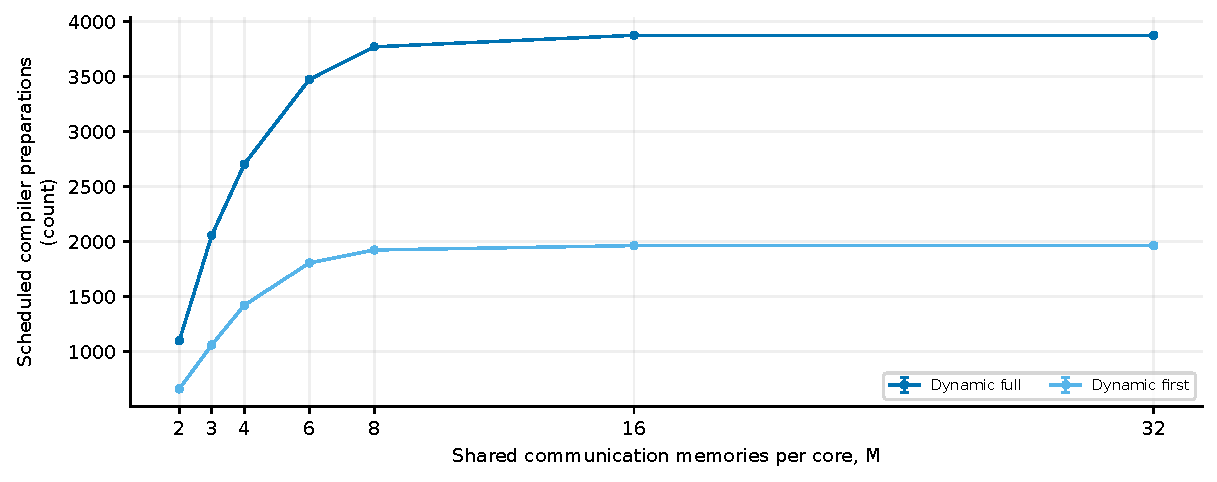
\includegraphics[width=.94\linewidth,height=.255\textheight,keepaspectratio]{figures/memory/mesh_xy_scheduled_preparations.pdf}\captionof{figure}{Run-level mean and sample SD. Shared trace aliases are counted once.}\end{center}
\begin{center}{\scriptsize\setlength{\tabcolsep}{3pt}
\begin{tabular}{lrrrrr}
\toprule
M & ODG & CGP & ACGP & Dynamic full & Dynamic first \\
\midrule
2 & n/a & n/a & n/a & $1101.00\pm0.00$ & $663.00\pm0.00$ \\
3 & n/a & n/a & n/a & $2059.00\pm0.00$ & $1063.00\pm0.00$ \\
4 & n/a & n/a & n/a & $2704.00\pm0.00$ & $1423.00\pm0.00$ \\
6 & n/a & n/a & n/a & $3474.00\pm0.00$ & $1807.00\pm0.00$ \\
8 & n/a & n/a & n/a & $3771.00\pm0.00$ & $1925.00\pm0.00$ \\
16 & n/a & n/a & n/a & $3876.00\pm0.00$ & $1965.00\pm0.00$ \\
32 & n/a & n/a & n/a & $3876.00\pm0.00$ & $1965.00\pm0.00$ \\
\bottomrule\end{tabular}}
\captionof{table}{Mean $\pm$ sample SD; n/a denotes a metric outside that policy's instrumentation.}
{\footnotesize\href{https://github.com/sanjeevkrishnaa/Compiler-Driven-ACE/blob/codex/ace-scheduler-correctness/docs/latex/qft96_final/data/memory_mesh_xy_scheduled_preparations.csv}{Exact CSV values and sample counts}}
\end{center}
\subsection*{Planner-blocked preparations}
\begin{center}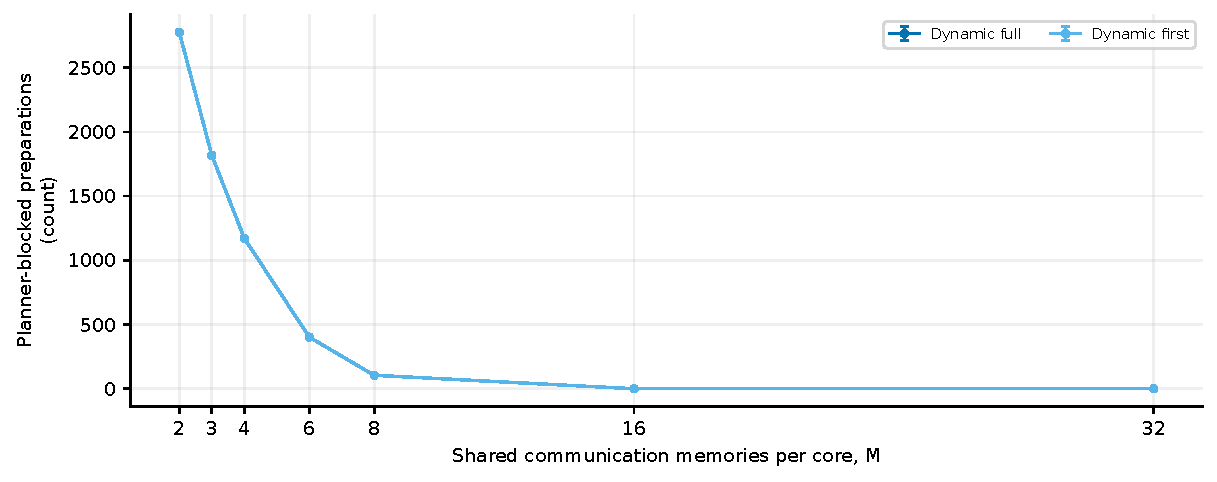
\includegraphics[width=.94\linewidth,height=.255\textheight,keepaspectratio]{figures/memory/mesh_xy_planner_blocked_preparations.pdf}\captionof{figure}{Run-level mean and sample SD. Shared trace aliases are counted once.}\end{center}
\begin{center}{\scriptsize\setlength{\tabcolsep}{3pt}
\begin{tabular}{lrrrrr}
\toprule
M & ODG & CGP & ACGP & Dynamic full & Dynamic first \\
\midrule
2 & n/a & n/a & n/a & $2775.00\pm0.00$ & $2775.00\pm0.00$ \\
3 & n/a & n/a & n/a & $1817.00\pm0.00$ & $1817.00\pm0.00$ \\
4 & n/a & n/a & n/a & $1172.00\pm0.00$ & $1172.00\pm0.00$ \\
6 & n/a & n/a & n/a & $402.00\pm0.00$ & $402.00\pm0.00$ \\
8 & n/a & n/a & n/a & $105.00\pm0.00$ & $105.00\pm0.00$ \\
16 & n/a & n/a & n/a & $0.0000\pm0.0000$ & $0.0000\pm0.0000$ \\
32 & n/a & n/a & n/a & $0.0000\pm0.0000$ & $0.0000\pm0.0000$ \\
\bottomrule\end{tabular}}
\captionof{table}{Mean $\pm$ sample SD; n/a denotes a metric outside that policy's instrumentation.}
{\footnotesize\href{https://github.com/sanjeevkrishnaa/Compiler-Driven-ACE/blob/codex/ace-scheduler-correctness/docs/latex/qft96_final/data/memory_mesh_xy_planner_blocked_preparations.csv}{Exact CSV values and sample counts}}
\end{center}
\clearpage
\subsection*{Planner peak compiler memory}
\begin{center}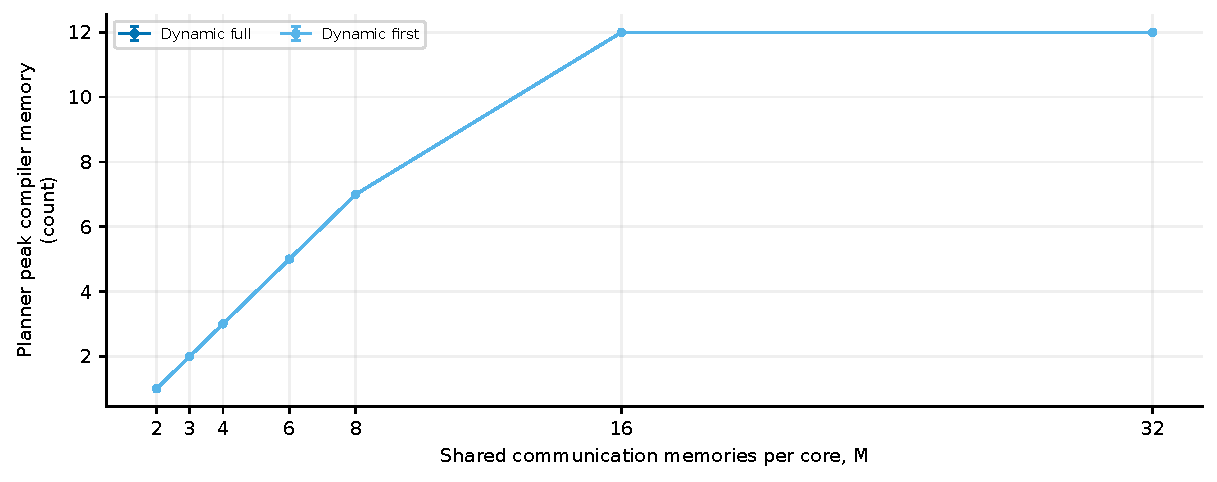
\includegraphics[width=.94\linewidth,height=.255\textheight,keepaspectratio]{figures/memory/mesh_xy_planner_peak_compiler_memory_per_core.pdf}\captionof{figure}{Run-level mean and sample SD. Shared trace aliases are counted once.}\end{center}
\begin{center}{\scriptsize\setlength{\tabcolsep}{3pt}
\begin{tabular}{lrrrrr}
\toprule
M & ODG & CGP & ACGP & Dynamic full & Dynamic first \\
\midrule
2 & n/a & n/a & n/a & $1.000\pm0.000$ & $1.000\pm0.000$ \\
3 & n/a & n/a & n/a & $2.000\pm0.000$ & $2.000\pm0.000$ \\
4 & n/a & n/a & n/a & $3.000\pm0.000$ & $3.000\pm0.000$ \\
6 & n/a & n/a & n/a & $5.000\pm0.000$ & $5.000\pm0.000$ \\
8 & n/a & n/a & n/a & $7.000\pm0.000$ & $7.000\pm0.000$ \\
16 & n/a & n/a & n/a & $12.000\pm0.000$ & $12.000\pm0.000$ \\
32 & n/a & n/a & n/a & $12.000\pm0.000$ & $12.000\pm0.000$ \\
\bottomrule\end{tabular}}
\captionof{table}{Mean $\pm$ sample SD; n/a denotes a metric outside that policy's instrumentation.}
{\footnotesize\href{https://github.com/sanjeevkrishnaa/Compiler-Driven-ACE/blob/codex/ace-scheduler-correctness/docs/latex/qft96_final/data/memory_mesh_xy_planner_peak_compiler_memory_per_core.csv}{Exact CSV values and sample counts}}
\end{center}
\subsection*{Compiler preparation admission attempts}
\begin{center}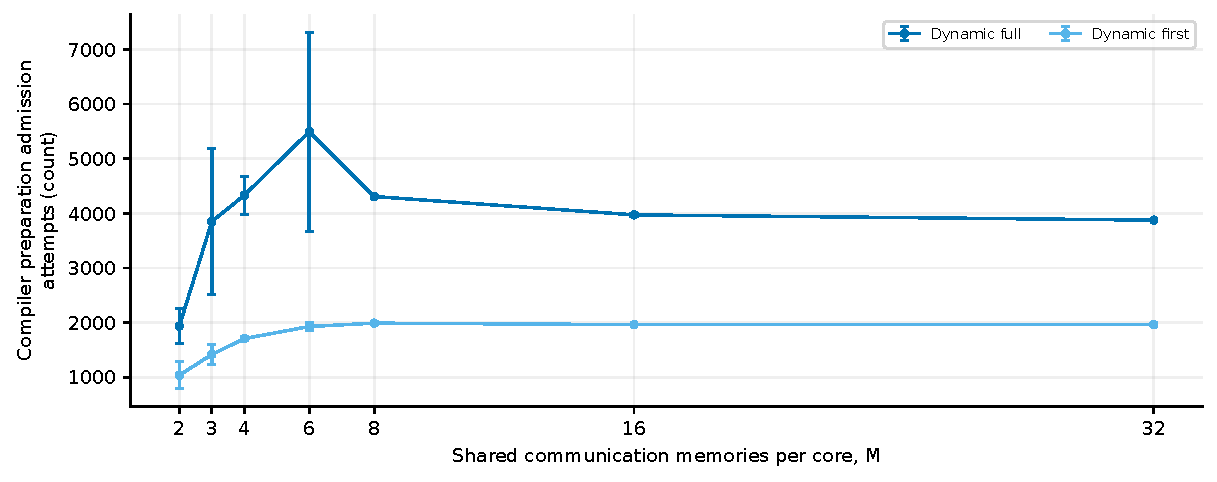
\includegraphics[width=.94\linewidth,height=.255\textheight,keepaspectratio]{figures/memory/mesh_xy_runtime_admission_attempts.pdf}\captionof{figure}{Run-level mean and sample SD. Shared trace aliases are counted once.}\end{center}
\begin{center}{\scriptsize\setlength{\tabcolsep}{3pt}
\begin{tabular}{lrrrrr}
\toprule
M & ODG & CGP & ACGP & Dynamic full & Dynamic first \\
\midrule
2 & n/a & n/a & n/a & $1937.50\pm317.49$ & $1039.00\pm247.49$ \\
3 & n/a & n/a & n/a & $3850.50\pm1332.90$ & $1418.50\pm190.21$ \\
4 & n/a & n/a & n/a & $4331.00\pm352.14$ & $1708.50\pm40.31$ \\
6 & n/a & n/a & n/a & $5494.50\pm1817.97$ & $1930.00\pm74.95$ \\
8 & n/a & n/a & n/a & $4308.00\pm22.63$ & $1992.00\pm21.21$ \\
16 & n/a & n/a & n/a & $3973.00\pm29.70$ & $1965.00\pm0.00$ \\
32 & n/a & n/a & n/a & $3876.00\pm0.00$ & $1965.00\pm0.00$ \\
\bottomrule\end{tabular}}
\captionof{table}{Mean $\pm$ sample SD; n/a denotes a metric outside that policy's instrumentation.}
{\footnotesize\href{https://github.com/sanjeevkrishnaa/Compiler-Driven-ACE/blob/codex/ace-scheduler-correctness/docs/latex/qft96_final/data/memory_mesh_xy_runtime_admission_attempts.csv}{Exact CSV values and sample counts}}
\end{center}
\clearpage
\subsection*{Launched compiler preparations}
\begin{center}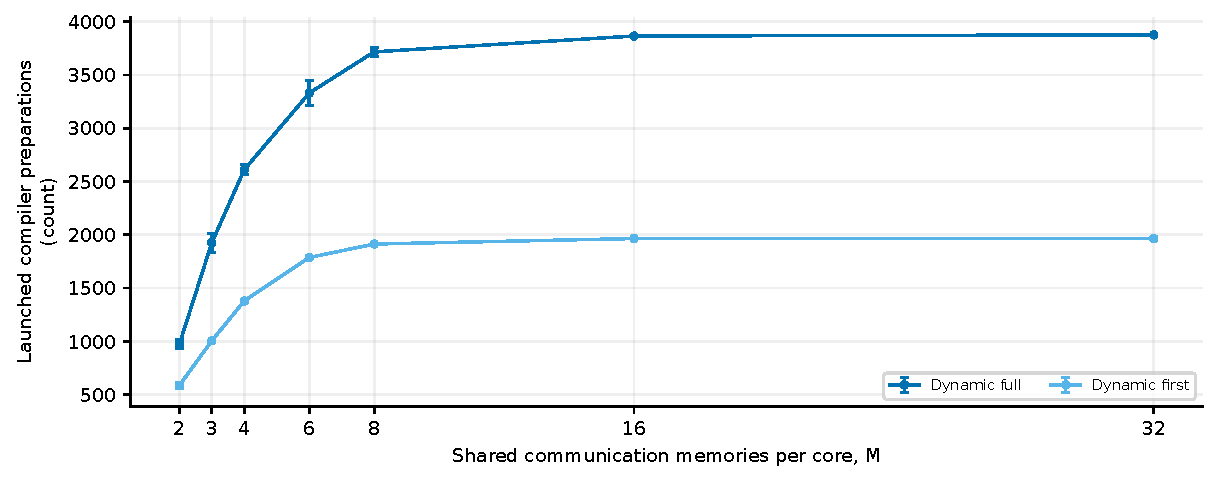
\includegraphics[width=.94\linewidth,height=.255\textheight,keepaspectratio]{figures/memory/mesh_xy_runtime_launched_preparations.pdf}\captionof{figure}{Run-level mean and sample SD. Shared trace aliases are counted once.}\end{center}
\begin{center}{\scriptsize\setlength{\tabcolsep}{3pt}
\begin{tabular}{lrrrrr}
\toprule
M & ODG & CGP & ACGP & Dynamic full & Dynamic first \\
\midrule
2 & n/a & n/a & n/a & $971.50\pm41.72$ & $586.50\pm31.82$ \\
3 & n/a & n/a & n/a & $1926.00\pm89.10$ & $1006.00\pm5.66$ \\
4 & n/a & n/a & n/a & $2611.00\pm49.50$ & $1379.50\pm17.68$ \\
6 & n/a & n/a & n/a & $3330.00\pm114.55$ & $1787.00\pm11.31$ \\
8 & n/a & n/a & n/a & $3716.50\pm40.31$ & $1913.50\pm6.36$ \\
16 & n/a & n/a & n/a & $3865.00\pm5.66$ & $1965.00\pm0.00$ \\
32 & n/a & n/a & n/a & $3876.00\pm0.00$ & $1965.00\pm0.00$ \\
\bottomrule\end{tabular}}
\captionof{table}{Mean $\pm$ sample SD; n/a denotes a metric outside that policy's instrumentation.}
{\footnotesize\href{https://github.com/sanjeevkrishnaa/Compiler-Driven-ACE/blob/codex/ace-scheduler-correctness/docs/latex/qft96_final/data/memory_mesh_xy_runtime_launched_preparations.csv}{Exact CSV values and sample counts}}
\end{center}
\subsection*{Accepted compiler preparations}
\begin{center}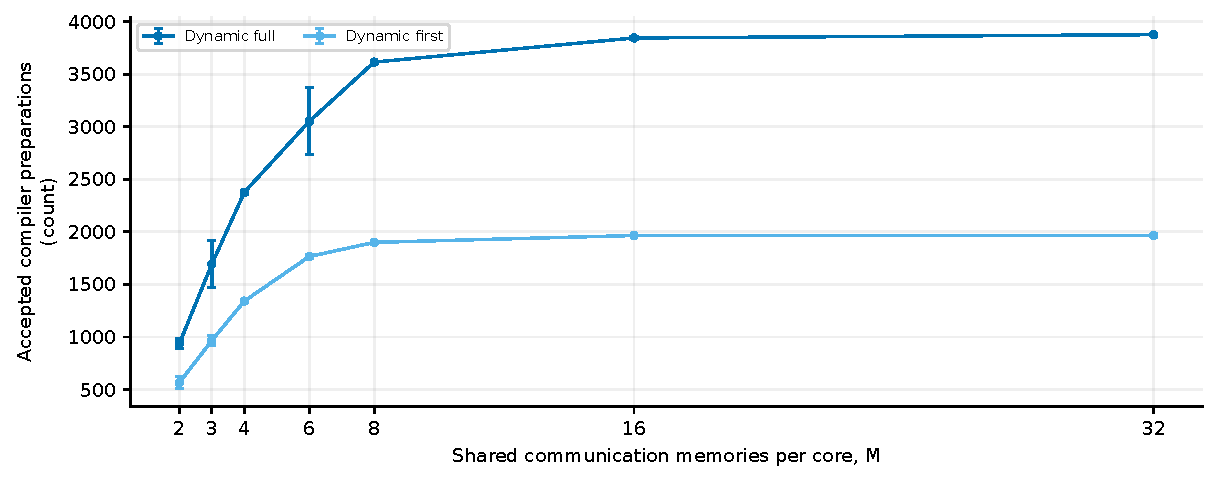
\includegraphics[width=.94\linewidth,height=.255\textheight,keepaspectratio]{figures/memory/mesh_xy_runtime_accepted_preparations.pdf}\captionof{figure}{Run-level mean and sample SD. Shared trace aliases are counted once.}\end{center}
\begin{center}{\scriptsize\setlength{\tabcolsep}{3pt}
\begin{tabular}{lrrrrr}
\toprule
M & ODG & CGP & ACGP & Dynamic full & Dynamic first \\
\midrule
2 & n/a & n/a & n/a & $935.00\pm45.25$ & $564.50\pm58.69$ \\
3 & n/a & n/a & n/a & $1692.50\pm221.32$ & $965.50\pm44.55$ \\
4 & n/a & n/a & n/a & $2375.50\pm16.26$ & $1340.50\pm12.02$ \\
6 & n/a & n/a & n/a & $3050.50\pm318.91$ & $1765.00\pm18.38$ \\
8 & n/a & n/a & n/a & $3615.00\pm8.49$ & $1899.50\pm3.54$ \\
16 & n/a & n/a & n/a & $3844.50\pm10.61$ & $1965.00\pm0.00$ \\
32 & n/a & n/a & n/a & $3876.00\pm0.00$ & $1965.00\pm0.00$ \\
\bottomrule\end{tabular}}
\captionof{table}{Mean $\pm$ sample SD; n/a denotes a metric outside that policy's instrumentation.}
{\footnotesize\href{https://github.com/sanjeevkrishnaa/Compiler-Driven-ACE/blob/codex/ace-scheduler-correctness/docs/latex/qft96_final/data/memory_mesh_xy_runtime_accepted_preparations.csv}{Exact CSV values and sample counts}}
\end{center}
\clearpage
\subsection*{Rejected compiler preparations}
\begin{center}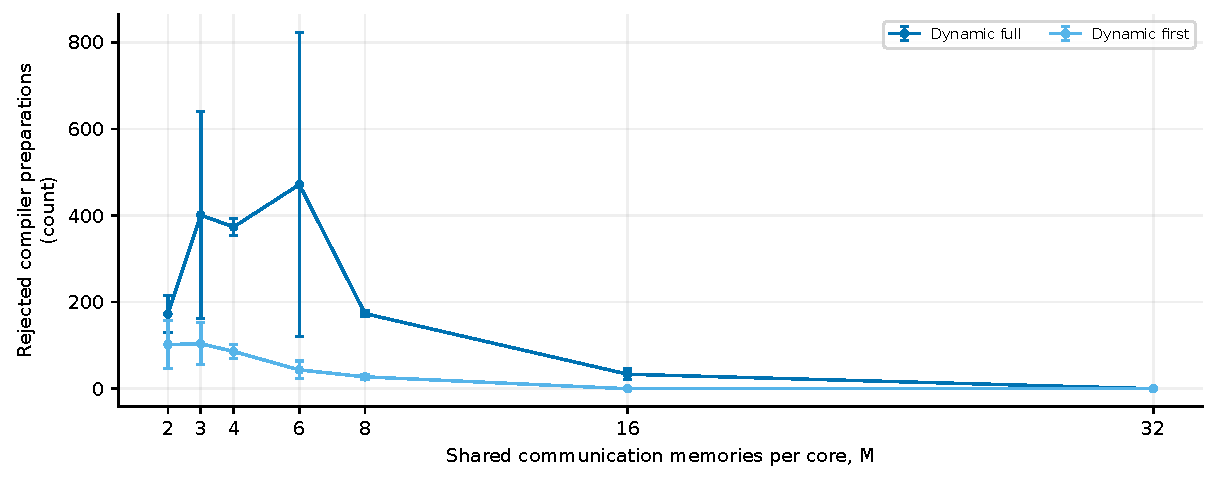
\includegraphics[width=.94\linewidth,height=.255\textheight,keepaspectratio]{figures/memory/mesh_xy_runtime_rejected_preparations.pdf}\captionof{figure}{Run-level mean and sample SD. Shared trace aliases are counted once.}\end{center}
\begin{center}{\scriptsize\setlength{\tabcolsep}{3pt}
\begin{tabular}{lrrrrr}
\toprule
M & ODG & CGP & ACGP & Dynamic full & Dynamic first \\
\midrule
2 & n/a & n/a & n/a & $172.50\pm43.13$ & $102.00\pm55.15$ \\
3 & n/a & n/a & n/a & $401.00\pm239.00$ & $104.00\pm48.08$ \\
4 & n/a & n/a & n/a & $373.50\pm19.09$ & $86.000\pm16.971$ \\
6 & n/a & n/a & n/a & $471.50\pm351.43$ & $43.500\pm20.506$ \\
8 & n/a & n/a & n/a & $173.50\pm6.36$ & $27.500\pm4.950$ \\
16 & n/a & n/a & n/a & $33.500\pm12.021$ & $0.0000\pm0.0000$ \\
32 & n/a & n/a & n/a & $0.0000\pm0.0000$ & $0.0000\pm0.0000$ \\
\bottomrule\end{tabular}}
\captionof{table}{Mean $\pm$ sample SD; n/a denotes a metric outside that policy's instrumentation.}
{\footnotesize\href{https://github.com/sanjeevkrishnaa/Compiler-Driven-ACE/blob/codex/ace-scheduler-correctness/docs/latex/qft96_final/data/memory_mesh_xy_runtime_rejected_preparations.csv}{Exact CSV values and sample counts}}
\end{center}
\subsection*{Compiler-ready request count}
\begin{center}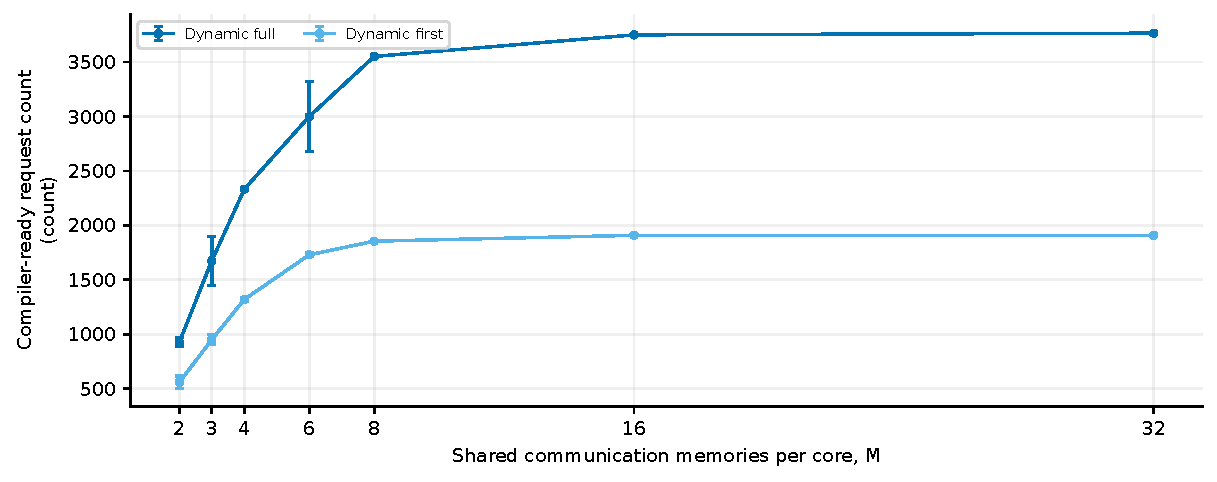
\includegraphics[width=.94\linewidth,height=.255\textheight,keepaspectratio]{figures/memory/mesh_xy_pregenerated_hits.pdf}\captionof{figure}{Run-level mean and sample SD. Shared trace aliases are counted once.}\end{center}
\begin{center}{\scriptsize\setlength{\tabcolsep}{3pt}
\begin{tabular}{lrrrrr}
\toprule
M & ODG & CGP & ACGP & Dynamic full & Dynamic first \\
\midrule
2 & n/a & n/a & n/a & $926.50\pm43.13$ & $557.50\pm58.69$ \\
3 & n/a & n/a & n/a & $1675.00\pm224.86$ & $950.00\pm46.67$ \\
4 & n/a & n/a & n/a & $2332.00\pm2.83$ & $1319.00\pm16.97$ \\
6 & n/a & n/a & n/a & $3000.00\pm323.85$ & $1729.50\pm16.26$ \\
8 & n/a & n/a & n/a & $3551.50\pm4.95$ & $1854.50\pm2.12$ \\
16 & n/a & n/a & n/a & $3750.00\pm1.41$ & $1908.50\pm3.54$ \\
32 & n/a & n/a & n/a & $3765.50\pm7.78$ & $1908.50\pm3.54$ \\
\bottomrule\end{tabular}}
\captionof{table}{Mean $\pm$ sample SD; n/a denotes a metric outside that policy's instrumentation.}
{\footnotesize\href{https://github.com/sanjeevkrishnaa/Compiler-Driven-ACE/blob/codex/ace-scheduler-correctness/docs/latex/qft96_final/data/memory_mesh_xy_pregenerated_hits.csv}{Exact CSV values and sample counts}}
\end{center}
\clearpage
\subsection*{Intended compiler-hit count}
\begin{center}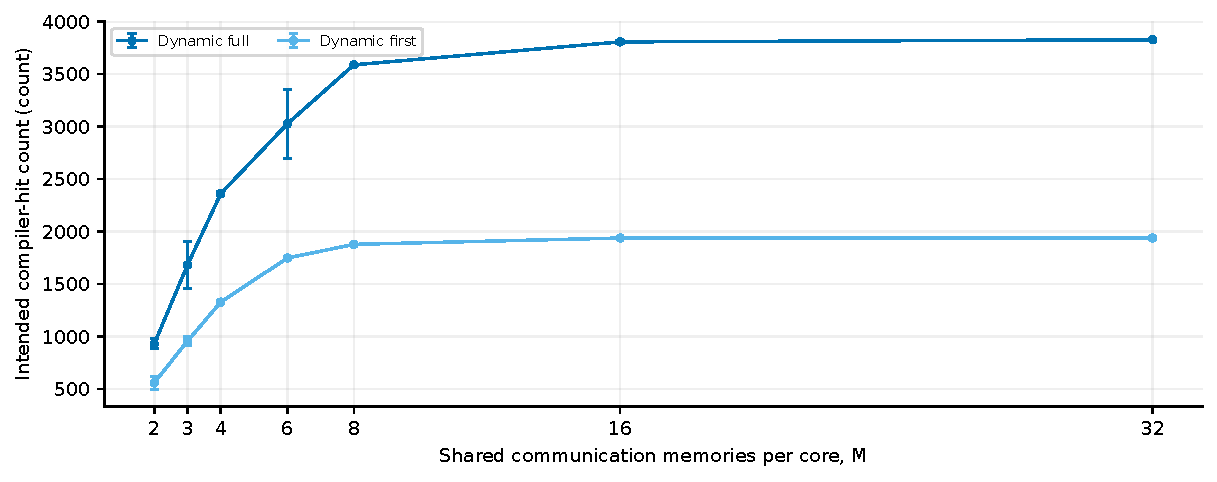
\includegraphics[width=.94\linewidth,height=.255\textheight,keepaspectratio]{figures/memory/mesh_xy_intended_request_hits.pdf}\captionof{figure}{Run-level mean and sample SD. Shared trace aliases are counted once.}\end{center}
\begin{center}{\scriptsize\setlength{\tabcolsep}{3pt}
\begin{tabular}{lrrrrr}
\toprule
M & ODG & CGP & ACGP & Dynamic full & Dynamic first \\
\midrule
2 & n/a & n/a & n/a & $931.00\pm46.67$ & $560.50\pm60.10$ \\
3 & n/a & n/a & n/a & $1683.00\pm226.27$ & $958.00\pm46.67$ \\
4 & n/a & n/a & n/a & $2362.00\pm16.97$ & $1329.00\pm12.73$ \\
6 & n/a & n/a & n/a & $3026.50\pm328.80$ & $1748.50\pm14.85$ \\
8 & n/a & n/a & n/a & $3588.50\pm6.36$ & $1878.50\pm0.71$ \\
16 & n/a & n/a & n/a & $3807.00\pm12.73$ & $1939.00\pm1.41$ \\
32 & n/a & n/a & n/a & $3827.50\pm6.36$ & $1939.00\pm1.41$ \\
\bottomrule\end{tabular}}
\captionof{table}{Mean $\pm$ sample SD; n/a denotes a metric outside that policy's instrumentation.}
{\footnotesize\href{https://github.com/sanjeevkrishnaa/Compiler-Driven-ACE/blob/codex/ace-scheduler-correctness/docs/latex/qft96_final/data/memory_mesh_xy_intended_request_hits.csv}{Exact CSV values and sample counts}}
\end{center}
\subsection*{Compiler-not-ready request count}
\begin{center}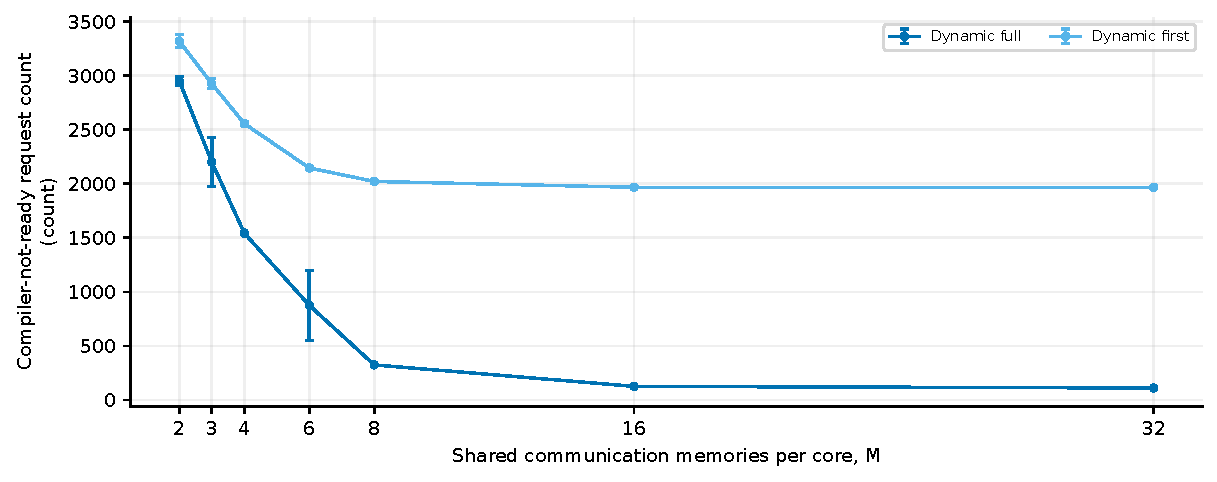
\includegraphics[width=.94\linewidth,height=.255\textheight,keepaspectratio]{figures/memory/mesh_xy_compiler_not_ready_requests.pdf}\captionof{figure}{Run-level mean and sample SD. Shared trace aliases are counted once.}\end{center}
\begin{center}{\scriptsize\setlength{\tabcolsep}{3pt}
\begin{tabular}{lrrrrr}
\toprule
M & ODG & CGP & ACGP & Dynamic full & Dynamic first \\
\midrule
2 & n/a & n/a & n/a & $2949.50\pm43.13$ & $3318.50\pm58.69$ \\
3 & n/a & n/a & n/a & $2201.00\pm224.86$ & $2926.00\pm46.67$ \\
4 & n/a & n/a & n/a & $1544.00\pm2.83$ & $2557.00\pm16.97$ \\
6 & n/a & n/a & n/a & $876.00\pm323.85$ & $2146.50\pm16.26$ \\
8 & n/a & n/a & n/a & $324.50\pm4.95$ & $2021.50\pm2.12$ \\
16 & n/a & n/a & n/a & $126.00\pm1.41$ & $1967.50\pm3.54$ \\
32 & n/a & n/a & n/a & $110.50\pm7.78$ & $1967.50\pm3.54$ \\
\bottomrule\end{tabular}}
\captionof{table}{Mean $\pm$ sample SD; n/a denotes a metric outside that policy's instrumentation.}
{\footnotesize\href{https://github.com/sanjeevkrishnaa/Compiler-Driven-ACE/blob/codex/ace-scheduler-correctness/docs/latex/qft96_final/data/memory_mesh_xy_compiler_not_ready_requests.csv}{Exact CSV values and sample counts}}
\end{center}
\clearpage
\subsection*{Late compiler-pair uses}
\begin{center}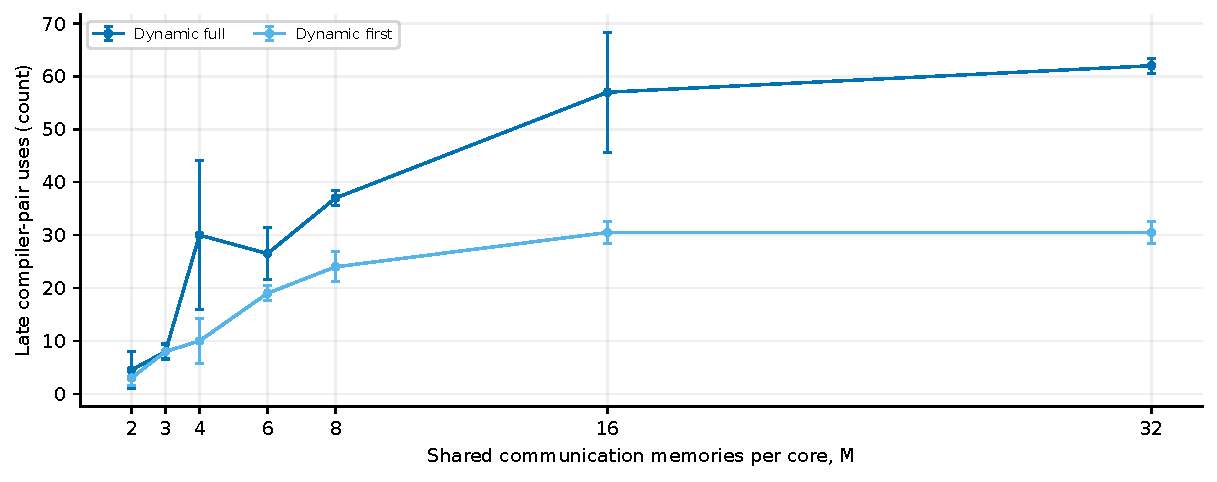
\includegraphics[width=.94\linewidth,height=.255\textheight,keepaspectratio]{figures/memory/mesh_xy_late_compiler_pair_uses.pdf}\captionof{figure}{Run-level mean and sample SD. Shared trace aliases are counted once.}\end{center}
\begin{center}{\scriptsize\setlength{\tabcolsep}{3pt}
\begin{tabular}{lrrrrr}
\toprule
M & ODG & CGP & ACGP & Dynamic full & Dynamic first \\
\midrule
2 & n/a & n/a & n/a & $4.500\pm3.536$ & $3.000\pm1.414$ \\
3 & n/a & n/a & n/a & $8.000\pm1.414$ & $8.000\pm0.000$ \\
4 & n/a & n/a & n/a & $30.000\pm14.142$ & $10.000\pm4.243$ \\
6 & n/a & n/a & n/a & $26.500\pm4.950$ & $19.000\pm1.414$ \\
8 & n/a & n/a & n/a & $37.000\pm1.414$ & $24.000\pm2.828$ \\
16 & n/a & n/a & n/a & $57.000\pm11.314$ & $30.500\pm2.121$ \\
32 & n/a & n/a & n/a & $62.000\pm1.414$ & $30.500\pm2.121$ \\
\bottomrule\end{tabular}}
\captionof{table}{Mean $\pm$ sample SD; n/a denotes a metric outside that policy's instrumentation.}
{\footnotesize\href{https://github.com/sanjeevkrishnaa/Compiler-Driven-ACE/blob/codex/ace-scheduler-correctness/docs/latex/qft96_final/data/memory_mesh_xy_late_compiler_pair_uses.csv}{Exact CSV values and sample counts}}
\end{center}
\subsection*{Compiler fallback count}
\begin{center}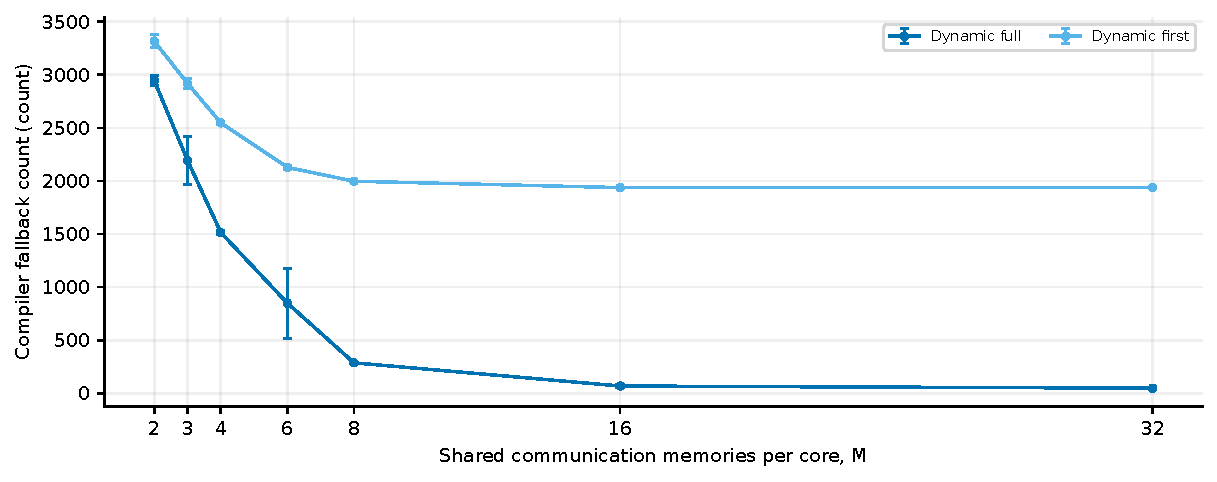
\includegraphics[width=.94\linewidth,height=.255\textheight,keepaspectratio]{figures/memory/mesh_xy_on_demand_fallbacks.pdf}\captionof{figure}{Run-level mean and sample SD. Shared trace aliases are counted once.}\end{center}
\begin{center}{\scriptsize\setlength{\tabcolsep}{3pt}
\begin{tabular}{lrrrrr}
\toprule
M & ODG & CGP & ACGP & Dynamic full & Dynamic first \\
\midrule
2 & n/a & n/a & n/a & $2945.00\pm46.67$ & $3315.50\pm60.10$ \\
3 & n/a & n/a & n/a & $2193.00\pm226.27$ & $2918.00\pm46.67$ \\
4 & n/a & n/a & n/a & $1514.00\pm16.97$ & $2547.00\pm12.73$ \\
6 & n/a & n/a & n/a & $849.50\pm328.80$ & $2127.50\pm14.85$ \\
8 & n/a & n/a & n/a & $287.50\pm6.36$ & $1997.50\pm0.71$ \\
16 & n/a & n/a & n/a & $69.000\pm12.728$ & $1937.00\pm1.41$ \\
32 & n/a & n/a & n/a & $48.500\pm6.364$ & $1937.00\pm1.41$ \\
\bottomrule\end{tabular}}
\captionof{table}{Mean $\pm$ sample SD; n/a denotes a metric outside that policy's instrumentation.}
{\footnotesize\href{https://github.com/sanjeevkrishnaa/Compiler-Driven-ACE/blob/codex/ace-scheduler-correctness/docs/latex/qft96_final/data/memory_mesh_xy_on_demand_fallbacks.csv}{Exact CSV values and sample counts}}
\end{center}
\clearpage
\subsection*{Generated compiler pairs}
\begin{center}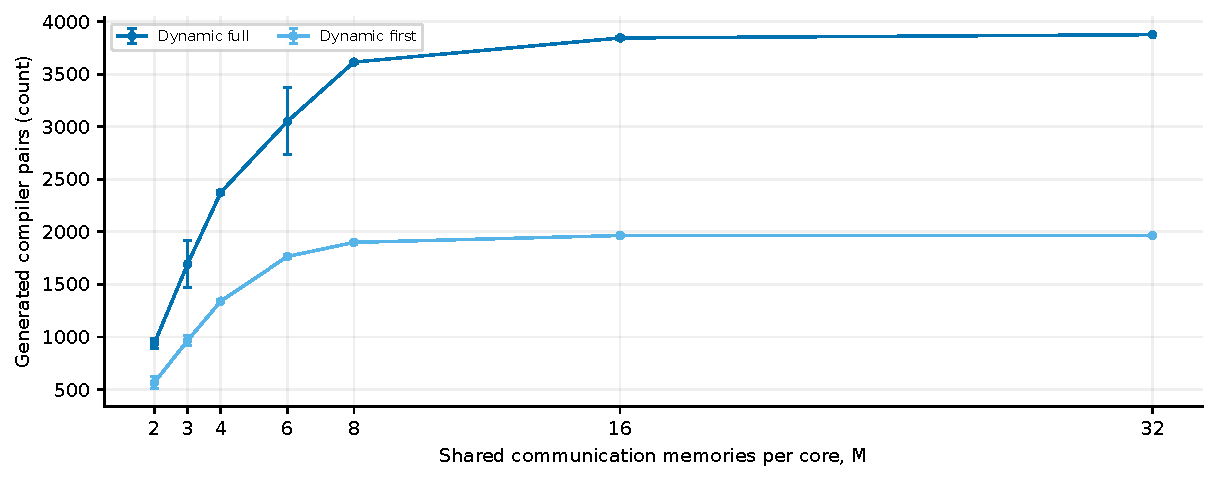
\includegraphics[width=.94\linewidth,height=.255\textheight,keepaspectratio]{figures/memory/mesh_xy_generated_compiler_pairs.pdf}\captionof{figure}{Run-level mean and sample SD. Shared trace aliases are counted once.}\end{center}
\begin{center}{\scriptsize\setlength{\tabcolsep}{3pt}
\begin{tabular}{lrrrrr}
\toprule
M & ODG & CGP & ACGP & Dynamic full & Dynamic first \\
\midrule
2 & n/a & n/a & n/a & $935.00\pm45.25$ & $564.50\pm58.69$ \\
3 & n/a & n/a & n/a & $1692.50\pm221.32$ & $965.50\pm44.55$ \\
4 & n/a & n/a & n/a & $2375.50\pm16.26$ & $1340.50\pm12.02$ \\
6 & n/a & n/a & n/a & $3050.50\pm318.91$ & $1765.00\pm18.38$ \\
8 & n/a & n/a & n/a & $3615.00\pm8.49$ & $1899.50\pm3.54$ \\
16 & n/a & n/a & n/a & $3844.50\pm10.61$ & $1965.00\pm0.00$ \\
32 & n/a & n/a & n/a & $3876.00\pm0.00$ & $1965.00\pm0.00$ \\
\bottomrule\end{tabular}}
\captionof{table}{Mean $\pm$ sample SD; n/a denotes a metric outside that policy's instrumentation.}
{\footnotesize\href{https://github.com/sanjeevkrishnaa/Compiler-Driven-ACE/blob/codex/ace-scheduler-correctness/docs/latex/qft96_final/data/memory_mesh_xy_generated_compiler_pairs.csv}{Exact CSV values and sample counts}}
\end{center}
\subsection*{Used compiler pairs}
\begin{center}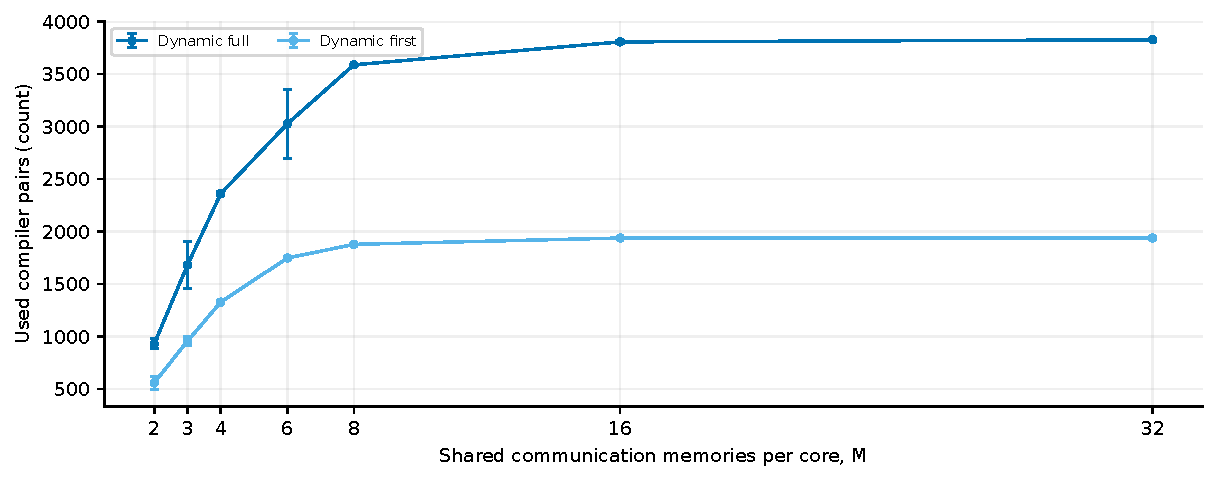
\includegraphics[width=.94\linewidth,height=.255\textheight,keepaspectratio]{figures/memory/mesh_xy_utilized_compiler_pairs.pdf}\captionof{figure}{Run-level mean and sample SD. Shared trace aliases are counted once.}\end{center}
\begin{center}{\scriptsize\setlength{\tabcolsep}{3pt}
\begin{tabular}{lrrrrr}
\toprule
M & ODG & CGP & ACGP & Dynamic full & Dynamic first \\
\midrule
2 & n/a & n/a & n/a & $931.00\pm46.67$ & $560.50\pm60.10$ \\
3 & n/a & n/a & n/a & $1683.00\pm226.27$ & $958.00\pm46.67$ \\
4 & n/a & n/a & n/a & $2362.00\pm16.97$ & $1329.00\pm12.73$ \\
6 & n/a & n/a & n/a & $3026.50\pm328.80$ & $1748.50\pm14.85$ \\
8 & n/a & n/a & n/a & $3588.50\pm6.36$ & $1878.50\pm0.71$ \\
16 & n/a & n/a & n/a & $3807.00\pm12.73$ & $1939.00\pm1.41$ \\
32 & n/a & n/a & n/a & $3827.50\pm6.36$ & $1939.00\pm1.41$ \\
\bottomrule\end{tabular}}
\captionof{table}{Mean $\pm$ sample SD; n/a denotes a metric outside that policy's instrumentation.}
{\footnotesize\href{https://github.com/sanjeevkrishnaa/Compiler-Driven-ACE/blob/codex/ace-scheduler-correctness/docs/latex/qft96_final/data/memory_mesh_xy_utilized_compiler_pairs.csv}{Exact CSV values and sample counts}}
\end{center}
\clearpage
\subsection*{Expired compiler pairs}
\begin{center}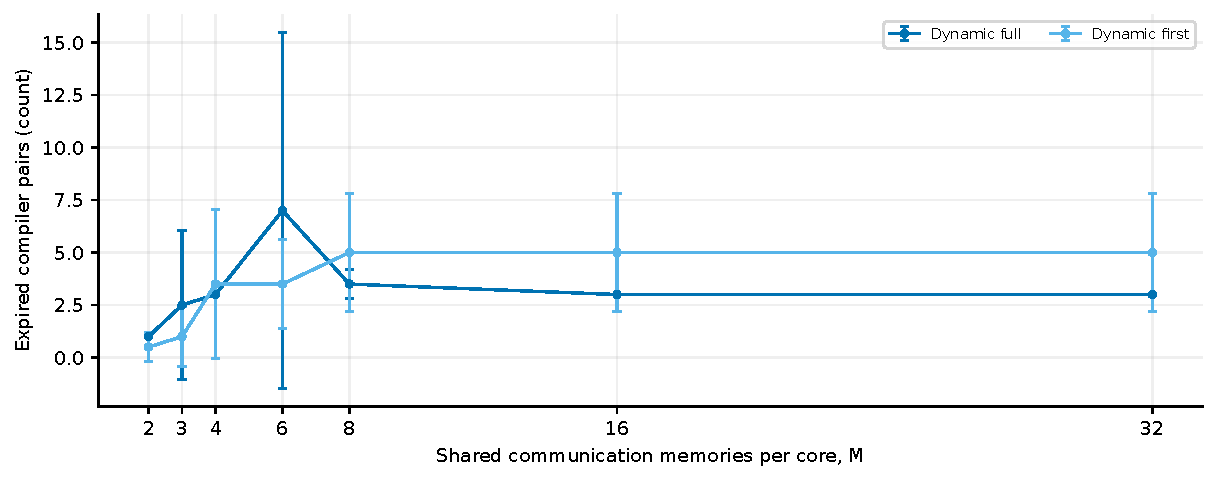
\includegraphics[width=.94\linewidth,height=.255\textheight,keepaspectratio]{figures/memory/mesh_xy_expired_compiler_pairs.pdf}\captionof{figure}{Run-level mean and sample SD. Shared trace aliases are counted once.}\end{center}
\begin{center}{\scriptsize\setlength{\tabcolsep}{3pt}
\begin{tabular}{lrrrrr}
\toprule
M & ODG & CGP & ACGP & Dynamic full & Dynamic first \\
\midrule
2 & n/a & n/a & n/a & $1.000\pm0.000$ & $0.5000\pm0.7071$ \\
3 & n/a & n/a & n/a & $2.500\pm3.536$ & $1.000\pm1.414$ \\
4 & n/a & n/a & n/a & $3.000\pm0.000$ & $3.500\pm3.536$ \\
6 & n/a & n/a & n/a & $7.000\pm8.485$ & $3.500\pm2.121$ \\
8 & n/a & n/a & n/a & $3.500\pm0.707$ & $5.000\pm2.828$ \\
16 & n/a & n/a & n/a & $3.000\pm0.000$ & $5.000\pm2.828$ \\
32 & n/a & n/a & n/a & $3.000\pm0.000$ & $5.000\pm2.828$ \\
\bottomrule\end{tabular}}
\captionof{table}{Mean $\pm$ sample SD; n/a denotes a metric outside that policy's instrumentation.}
{\footnotesize\href{https://github.com/sanjeevkrishnaa/Compiler-Driven-ACE/blob/codex/ace-scheduler-correctness/docs/latex/qft96_final/data/memory_mesh_xy_expired_compiler_pairs.csv}{Exact CSV values and sample counts}}
\end{center}
\subsection*{Remaining compiler pairs}
\begin{center}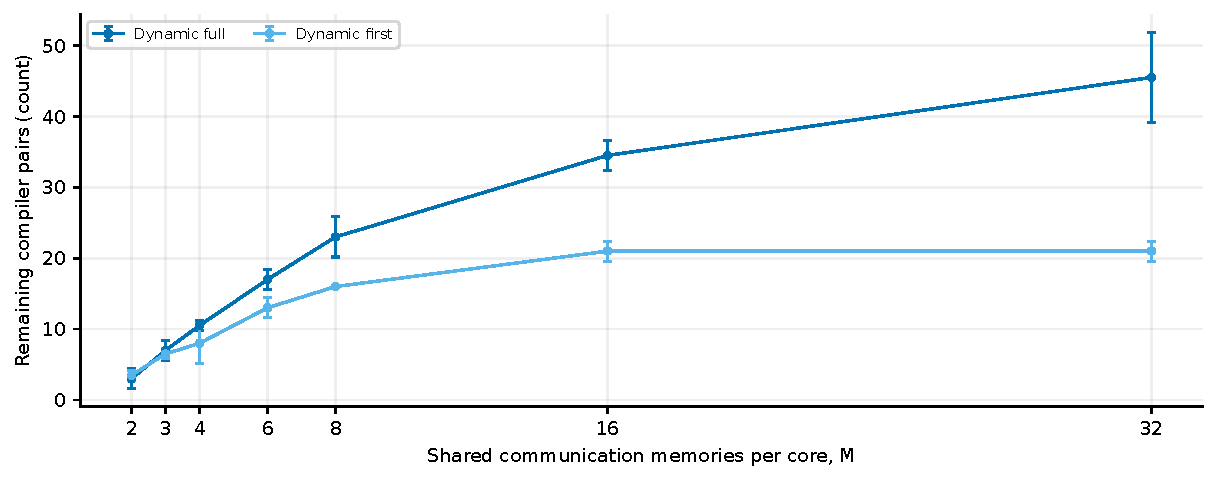
\includegraphics[width=.94\linewidth,height=.255\textheight,keepaspectratio]{figures/memory/mesh_xy_remaining_compiler_pairs.pdf}\captionof{figure}{Run-level mean and sample SD. Shared trace aliases are counted once.}\end{center}
\begin{center}{\scriptsize\setlength{\tabcolsep}{3pt}
\begin{tabular}{lrrrrr}
\toprule
M & ODG & CGP & ACGP & Dynamic full & Dynamic first \\
\midrule
2 & n/a & n/a & n/a & $3.000\pm1.414$ & $3.500\pm0.707$ \\
3 & n/a & n/a & n/a & $7.000\pm1.414$ & $6.500\pm0.707$ \\
4 & n/a & n/a & n/a & $10.500\pm0.707$ & $8.000\pm2.828$ \\
6 & n/a & n/a & n/a & $17.000\pm1.414$ & $13.000\pm1.414$ \\
8 & n/a & n/a & n/a & $23.000\pm2.828$ & $16.000\pm0.000$ \\
16 & n/a & n/a & n/a & $34.500\pm2.121$ & $21.000\pm1.414$ \\
32 & n/a & n/a & n/a & $45.500\pm6.364$ & $21.000\pm1.414$ \\
\bottomrule\end{tabular}}
\captionof{table}{Mean $\pm$ sample SD; n/a denotes a metric outside that policy's instrumentation.}
{\footnotesize\href{https://github.com/sanjeevkrishnaa/Compiler-Driven-ACE/blob/codex/ace-scheduler-correctness/docs/latex/qft96_final/data/memory_mesh_xy_remaining_compiler_pairs.csv}{Exact CSV values and sample counts}}
\end{center}
\clearpage
\subsection*{Compiler fidelity at creation}
\begin{center}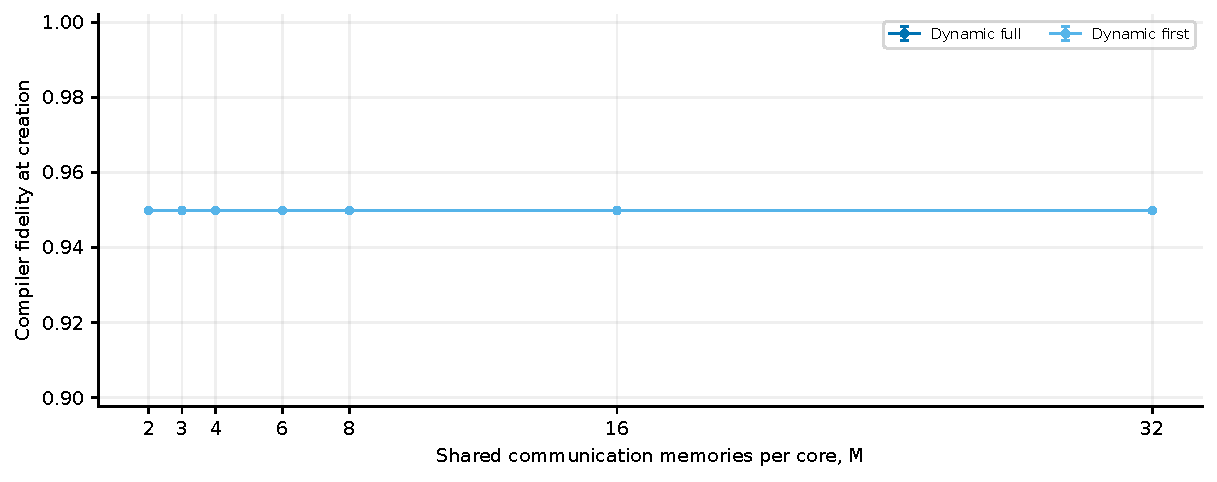
\includegraphics[width=.94\linewidth,height=.255\textheight,keepaspectratio]{figures/memory/mesh_xy_average_fidelity_at_creation.pdf}\captionof{figure}{Run-level mean and sample SD. Shared trace aliases are counted once.}\end{center}
\begin{center}{\scriptsize\setlength{\tabcolsep}{3pt}
\begin{tabular}{lrrrrr}
\toprule
M & ODG & CGP & ACGP & Dynamic full & Dynamic first \\
\midrule
2 & n/a & n/a & n/a & $0.9498\pm0.0000$ & $0.9498\pm0.0000$ \\
3 & n/a & n/a & n/a & $0.9498\pm0.0000$ & $0.9498\pm0.0000$ \\
4 & n/a & n/a & n/a & $0.9498\pm0.0000$ & $0.9498\pm0.0000$ \\
6 & n/a & n/a & n/a & $0.9498\pm0.0000$ & $0.9498\pm0.0000$ \\
8 & n/a & n/a & n/a & $0.9498\pm0.0000$ & $0.9498\pm0.0000$ \\
16 & n/a & n/a & n/a & $0.9498\pm0.0000$ & $0.9498\pm0.0000$ \\
32 & n/a & n/a & n/a & $0.9498\pm0.0000$ & $0.9498\pm0.0000$ \\
\bottomrule\end{tabular}}
\captionof{table}{Mean $\pm$ sample SD; n/a denotes a metric outside that policy's instrumentation.}
{\footnotesize\href{https://github.com/sanjeevkrishnaa/Compiler-Driven-ACE/blob/codex/ace-scheduler-correctness/docs/latex/qft96_final/data/memory_mesh_xy_average_fidelity_at_creation.csv}{Exact CSV values and sample counts}}
\end{center}
\subsection*{Compiler fidelity at use}
\begin{center}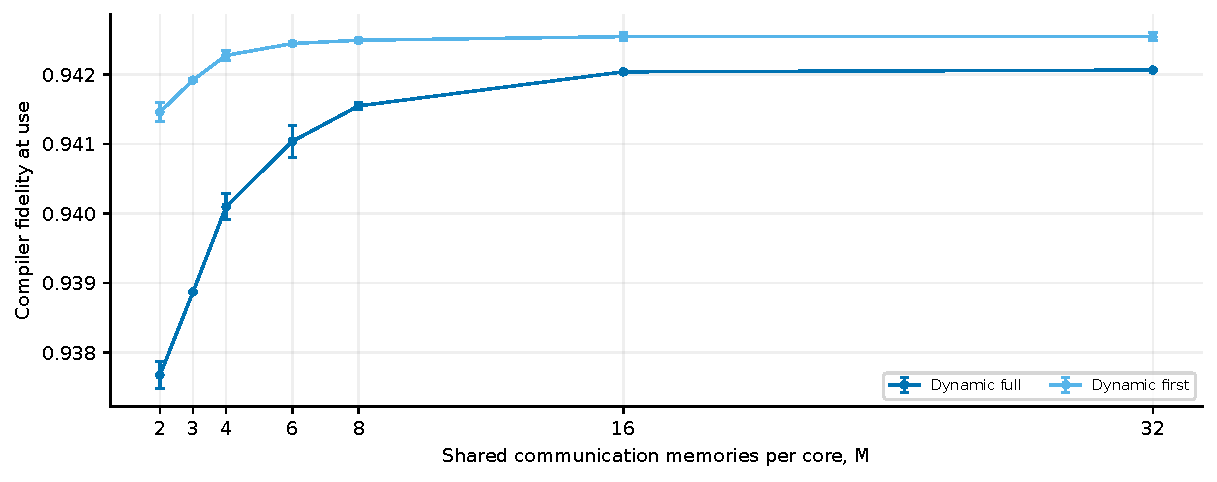
\includegraphics[width=.94\linewidth,height=.255\textheight,keepaspectratio]{figures/memory/mesh_xy_average_fidelity_at_utilization.pdf}\captionof{figure}{Run-level mean and sample SD. Shared trace aliases are counted once.}\end{center}
\begin{center}{\scriptsize\setlength{\tabcolsep}{3pt}
\begin{tabular}{lrrrrr}
\toprule
M & ODG & CGP & ACGP & Dynamic full & Dynamic first \\
\midrule
2 & n/a & n/a & n/a & $0.9377\pm0.0002$ & $0.9415\pm0.0001$ \\
3 & n/a & n/a & n/a & $0.9389\pm0.0000$ & $0.9419\pm0.0000$ \\
4 & n/a & n/a & n/a & $0.9401\pm0.0002$ & $0.9423\pm0.0001$ \\
6 & n/a & n/a & n/a & $0.9410\pm0.0002$ & $0.9424\pm0.0000$ \\
8 & n/a & n/a & n/a & $0.9415\pm0.0000$ & $0.9425\pm0.0000$ \\
16 & n/a & n/a & n/a & $0.9420\pm0.0000$ & $0.9425\pm0.0001$ \\
32 & n/a & n/a & n/a & $0.9421\pm0.0000$ & $0.9425\pm0.0001$ \\
\bottomrule\end{tabular}}
\captionof{table}{Mean $\pm$ sample SD; n/a denotes a metric outside that policy's instrumentation.}
{\footnotesize\href{https://github.com/sanjeevkrishnaa/Compiler-Driven-ACE/blob/codex/ace-scheduler-correctness/docs/latex/qft96_final/data/memory_mesh_xy_average_fidelity_at_utilization.csv}{Exact CSV values and sample counts}}
\end{center}
\clearpage
\subsection*{Mean layer latency}
\begin{center}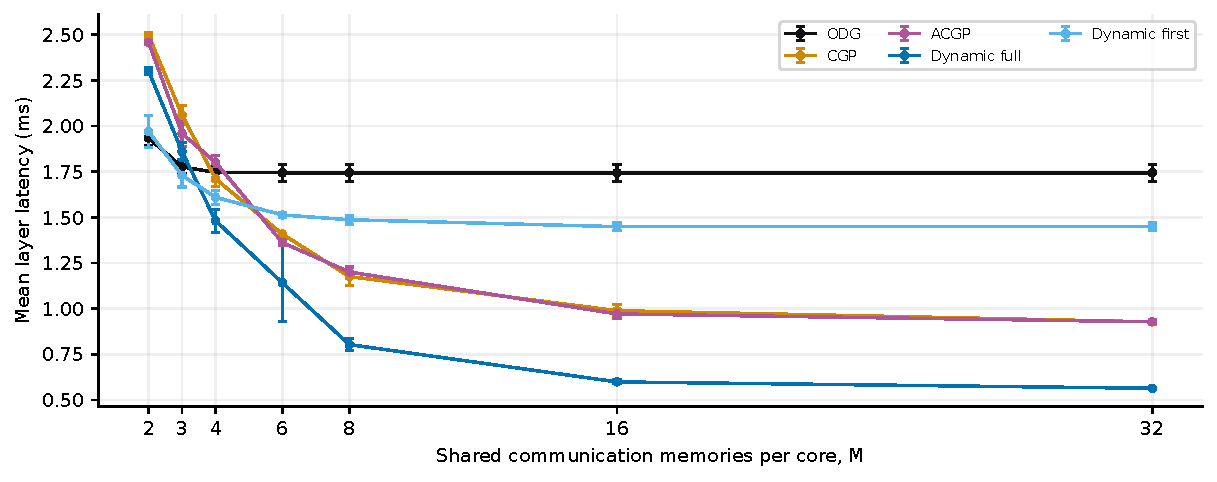
\includegraphics[width=.94\linewidth,height=.255\textheight,keepaspectratio]{figures/memory/mesh_xy_avg_layer_latency_ms.pdf}\captionof{figure}{Run-level mean and sample SD. Shared trace aliases are counted once.}\end{center}
\begin{center}{\scriptsize\setlength{\tabcolsep}{3pt}
\begin{tabular}{lrrrrr}
\toprule
M & ODG & CGP & ACGP & Dynamic full & Dynamic first \\
\midrule
2 & $1.935\pm0.040$ & $2.498\pm0.016$ & $2.458\pm0.010$ & $2.302\pm0.018$ & $1.971\pm0.088$ \\
3 & $1.777\pm0.034$ & $2.061\pm0.054$ & $1.959\pm0.071$ & $1.861\pm0.047$ & $1.731\pm0.064$ \\
4 & $1.746\pm0.040$ & $1.711\pm0.040$ & $1.802\pm0.036$ & $1.482\pm0.062$ & $1.610\pm0.038$ \\
6 & $1.744\pm0.047$ & $1.409\pm0.006$ & $1.362\pm0.017$ & $1.142\pm0.213$ & $1.514\pm0.012$ \\
8 & $1.744\pm0.047$ & $1.176\pm0.051$ & $1.201\pm0.028$ & $0.8035\pm0.0319$ & $1.487\pm0.025$ \\
16 & $1.744\pm0.047$ & $0.9892\pm0.0314$ & $0.9714\pm0.0233$ & $0.5992\pm0.0108$ & $1.449\pm0.020$ \\
32 & $1.744\pm0.047$ & $0.9280\pm0.0115$ & $0.9282\pm0.0099$ & $0.5641\pm0.0024$ & $1.449\pm0.020$ \\
\bottomrule\end{tabular}}
\captionof{table}{Mean $\pm$ sample SD; n/a denotes a metric outside that policy's instrumentation.}
{\footnotesize\href{https://github.com/sanjeevkrishnaa/Compiler-Driven-ACE/blob/codex/ace-scheduler-correctness/docs/latex/qft96_final/data/memory_mesh_xy_avg_layer_latency_ms.csv}{Exact CSV values and sample counts}}
\end{center}
\subsection*{Maximum layer latency}
\begin{center}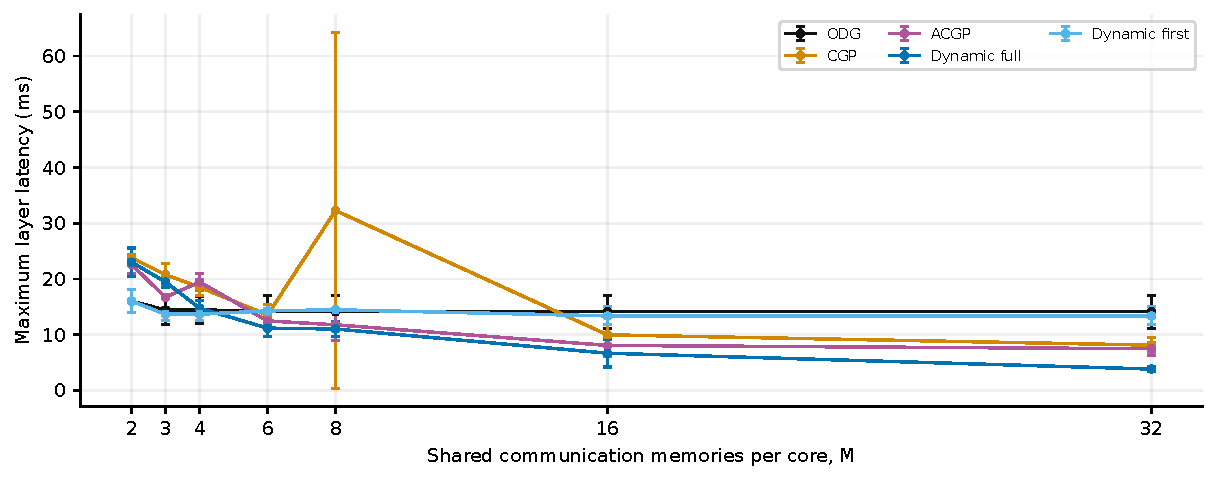
\includegraphics[width=.94\linewidth,height=.255\textheight,keepaspectratio]{figures/memory/mesh_xy_max_layer_latency_ms.pdf}\captionof{figure}{Run-level mean and sample SD. Shared trace aliases are counted once.}\end{center}
\begin{center}{\scriptsize\setlength{\tabcolsep}{3pt}
\begin{tabular}{lrrrrr}
\toprule
M & ODG & CGP & ACGP & Dynamic full & Dynamic first \\
\midrule
2 & $16.000\pm0.283$ & $23.801\pm0.566$ & $22.551\pm1.626$ & $23.001\pm2.546$ & $16.000\pm2.121$ \\
3 & $14.400\pm2.546$ & $20.750\pm2.051$ & $16.700\pm0.141$ & $19.450\pm0.919$ & $13.650\pm1.202$ \\
4 & $14.450\pm2.475$ & $18.518\pm1.439$ & $19.450\pm1.485$ & $14.750\pm1.344$ & $13.650\pm1.202$ \\
6 & $14.100\pm2.970$ & $13.500\pm1.980$ & $12.450\pm0.778$ & $11.150\pm1.485$ & $14.250\pm0.354$ \\
8 & $14.100\pm2.970$ & $32.271\pm32.003$ & $11.750\pm2.899$ & $11.000\pm1.273$ & $14.450\pm0.071$ \\
16 & $14.100\pm2.970$ & $9.950\pm3.748$ & $8.050\pm2.051$ & $6.650\pm2.475$ & $13.350\pm1.626$ \\
32 & $14.100\pm2.970$ & $8.100\pm1.414$ & $7.450\pm1.202$ & $3.800\pm0.424$ & $13.350\pm1.626$ \\
\bottomrule\end{tabular}}
\captionof{table}{Mean $\pm$ sample SD; n/a denotes a metric outside that policy's instrumentation.}
{\footnotesize\href{https://github.com/sanjeevkrishnaa/Compiler-Driven-ACE/blob/codex/ace-scheduler-correctness/docs/latex/qft96_final/data/memory_mesh_xy_max_layer_latency_ms.csv}{Exact CSV values and sample counts}}
\end{center}
\clearpage
\subsection*{Minimum layer latency}
\begin{center}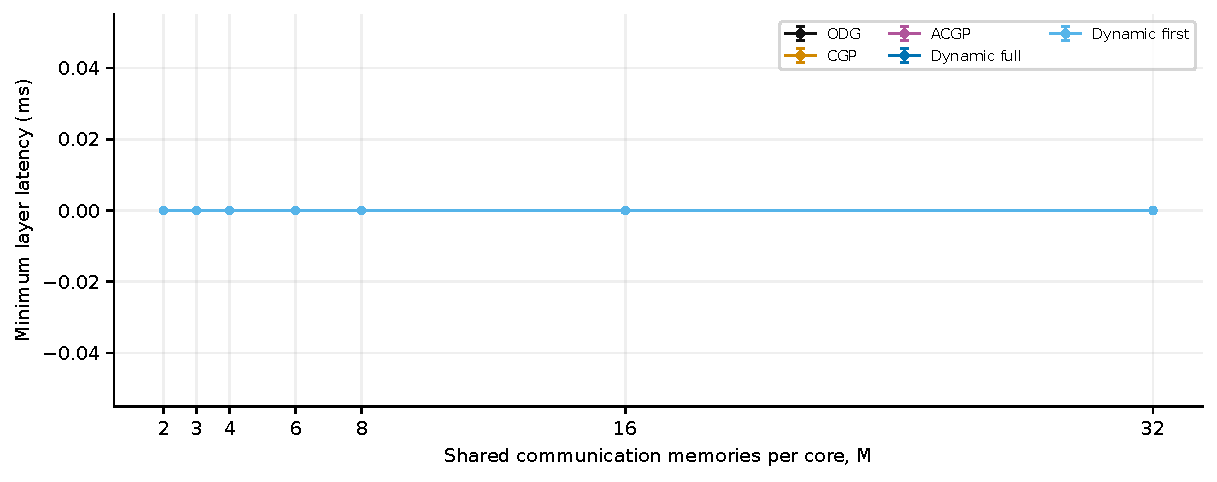
\includegraphics[width=.94\linewidth,height=.255\textheight,keepaspectratio]{figures/memory/mesh_xy_min_layer_latency_ms.pdf}\captionof{figure}{Run-level mean and sample SD. Shared trace aliases are counted once.}\end{center}
\begin{center}{\scriptsize\setlength{\tabcolsep}{3pt}
\begin{tabular}{lrrrrr}
\toprule
M & ODG & CGP & ACGP & Dynamic full & Dynamic first \\
\midrule
2 & $0.0000\pm0.0000$ & $0.0000\pm0.0000$ & $0.0000\pm0.0000$ & $0.0000\pm0.0000$ & $0.0000\pm0.0000$ \\
3 & $0.0000\pm0.0000$ & $0.0000\pm0.0000$ & $0.0000\pm0.0000$ & $0.0000\pm0.0000$ & $0.0000\pm0.0000$ \\
4 & $0.0000\pm0.0000$ & $0.0000\pm0.0000$ & $0.0000\pm0.0000$ & $0.0000\pm0.0000$ & $0.0000\pm0.0000$ \\
6 & $0.0000\pm0.0000$ & $0.0000\pm0.0000$ & $0.0000\pm0.0000$ & $0.0000\pm0.0000$ & $0.0000\pm0.0000$ \\
8 & $0.0000\pm0.0000$ & $0.0000\pm0.0000$ & $0.0000\pm0.0000$ & $0.0000\pm0.0000$ & $0.0000\pm0.0000$ \\
16 & $0.0000\pm0.0000$ & $0.0000\pm0.0000$ & $0.0000\pm0.0000$ & $0.0000\pm0.0000$ & $0.0000\pm0.0000$ \\
32 & $0.0000\pm0.0000$ & $0.0000\pm0.0000$ & $0.0000\pm0.0000$ & $0.0000\pm0.0000$ & $0.0000\pm0.0000$ \\
\bottomrule\end{tabular}}
\captionof{table}{Mean $\pm$ sample SD; n/a denotes a metric outside that policy's instrumentation.}
{\footnotesize\href{https://github.com/sanjeevkrishnaa/Compiler-Driven-ACE/blob/codex/ace-scheduler-correctness/docs/latex/qft96_final/data/memory_mesh_xy_min_layer_latency_ms.csv}{Exact CSV values and sample counts}}
\end{center}
\section{YX}
\clearpage
\subsection*{Mean request latency}
\begin{center}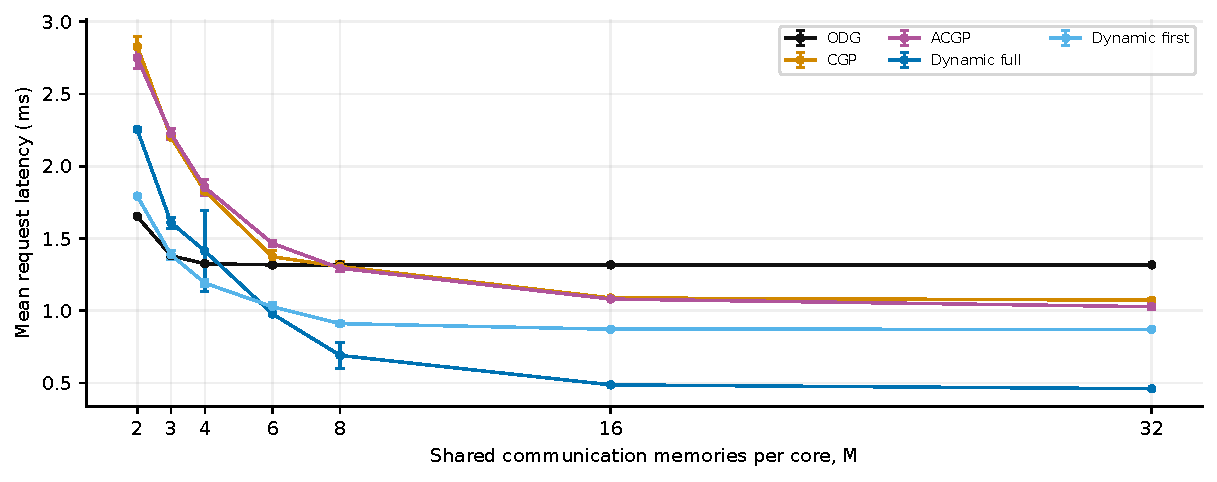
\includegraphics[width=.94\linewidth,height=.255\textheight,keepaspectratio]{figures/memory/mesh_yx_request_latency_mean_ms.pdf}\captionof{figure}{Run-level mean and sample SD. Shared trace aliases are counted once.}\end{center}
\begin{center}{\scriptsize\setlength{\tabcolsep}{3pt}
\begin{tabular}{lrrrrr}
\toprule
M & ODG & CGP & ACGP & Dynamic full & Dynamic first \\
\midrule
2 & $1.653\pm0.005$ & $2.827\pm0.069$ & $2.751\pm0.076$ & $2.254\pm0.014$ & $1.793\pm0.008$ \\
3 & $1.381\pm0.005$ & $2.202\pm0.010$ & $2.224\pm0.040$ & $1.610\pm0.038$ & $1.387\pm0.033$ \\
4 & $1.326\pm0.001$ & $1.828\pm0.019$ & $1.854\pm0.055$ & $1.414\pm0.282$ & $1.192\pm0.025$ \\
6 & $1.318\pm0.000$ & $1.374\pm0.044$ & $1.466\pm0.019$ & $0.9785\pm0.0017$ & $1.029\pm0.030$ \\
8 & $1.318\pm0.000$ & $1.307\pm0.037$ & $1.295\pm0.026$ & $0.6916\pm0.0885$ & $0.9115\pm0.0118$ \\
16 & $1.318\pm0.000$ & $1.089\pm0.001$ & $1.081\pm0.005$ & $0.4880\pm0.0003$ & $0.8725\pm0.0012$ \\
32 & $1.318\pm0.000$ & $1.073\pm0.012$ & $1.028\pm0.019$ & $0.4607\pm0.0012$ & $0.8724\pm0.0011$ \\
\bottomrule\end{tabular}}
\captionof{table}{Mean $\pm$ sample SD; n/a denotes a metric outside that policy's instrumentation.}
{\footnotesize\href{https://github.com/sanjeevkrishnaa/Compiler-Driven-ACE/blob/codex/ace-scheduler-correctness/docs/latex/qft96_final/data/memory_mesh_yx_request_latency_mean_ms.csv}{Exact CSV values and sample counts}}
\end{center}
\subsection*{Median request latency}
\begin{center}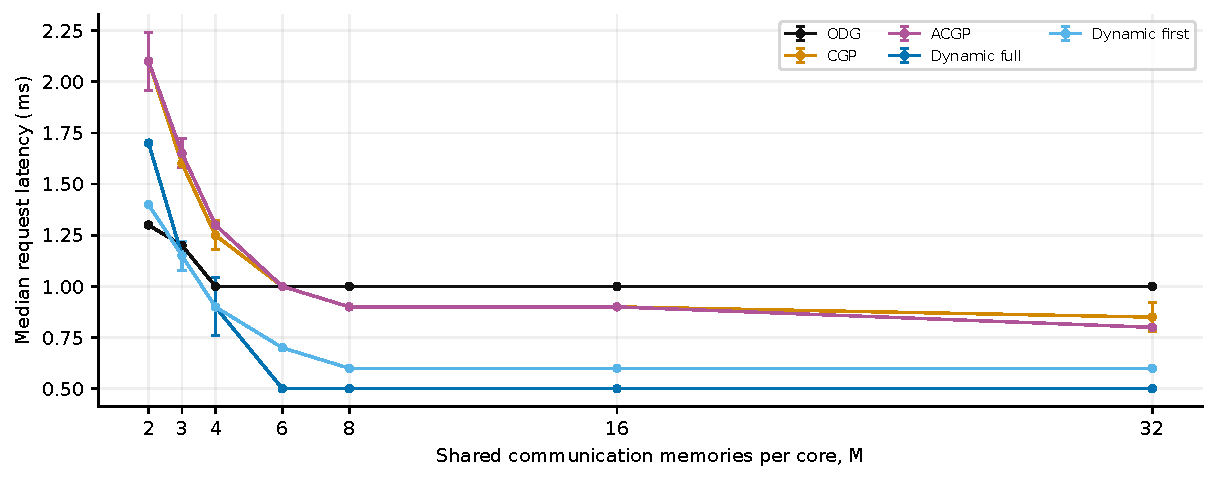
\includegraphics[width=.94\linewidth,height=.255\textheight,keepaspectratio]{figures/memory/mesh_yx_request_latency_median_ms.pdf}\captionof{figure}{Run-level mean and sample SD. Shared trace aliases are counted once.}\end{center}
\begin{center}{\scriptsize\setlength{\tabcolsep}{3pt}
\begin{tabular}{lrrrrr}
\toprule
M & ODG & CGP & ACGP & Dynamic full & Dynamic first \\
\midrule
2 & $1.300\pm0.000$ & $2.100\pm0.000$ & $2.100\pm0.141$ & $1.700\pm0.000$ & $1.400\pm0.000$ \\
3 & $1.200\pm0.000$ & $1.600\pm0.000$ & $1.650\pm0.071$ & $1.150\pm0.071$ & $1.150\pm0.071$ \\
4 & $1.000\pm0.000$ & $1.250\pm0.071$ & $1.300\pm0.000$ & $0.9000\pm0.1414$ & $0.9000\pm0.0000$ \\
6 & $1.000\pm0.000$ & $1.000\pm0.000$ & $1.000\pm0.000$ & $0.5000\pm0.0000$ & $0.7000\pm0.0000$ \\
8 & $1.000\pm0.000$ & $0.9000\pm0.0000$ & $0.9000\pm0.0000$ & $0.5000\pm0.0000$ & $0.6000\pm0.0000$ \\
16 & $1.000\pm0.000$ & $0.9000\pm0.0000$ & $0.9000\pm0.0000$ & $0.5000\pm0.0000$ & $0.6000\pm0.0000$ \\
32 & $1.000\pm0.000$ & $0.8500\pm0.0707$ & $0.8000\pm0.0000$ & $0.5000\pm0.0000$ & $0.6000\pm0.0000$ \\
\bottomrule\end{tabular}}
\captionof{table}{Mean $\pm$ sample SD; n/a denotes a metric outside that policy's instrumentation.}
{\footnotesize\href{https://github.com/sanjeevkrishnaa/Compiler-Driven-ACE/blob/codex/ace-scheduler-correctness/docs/latex/qft96_final/data/memory_mesh_yx_request_latency_median_ms.csv}{Exact CSV values and sample counts}}
\end{center}
\clearpage
\subsection*{p95 request latency}
\begin{center}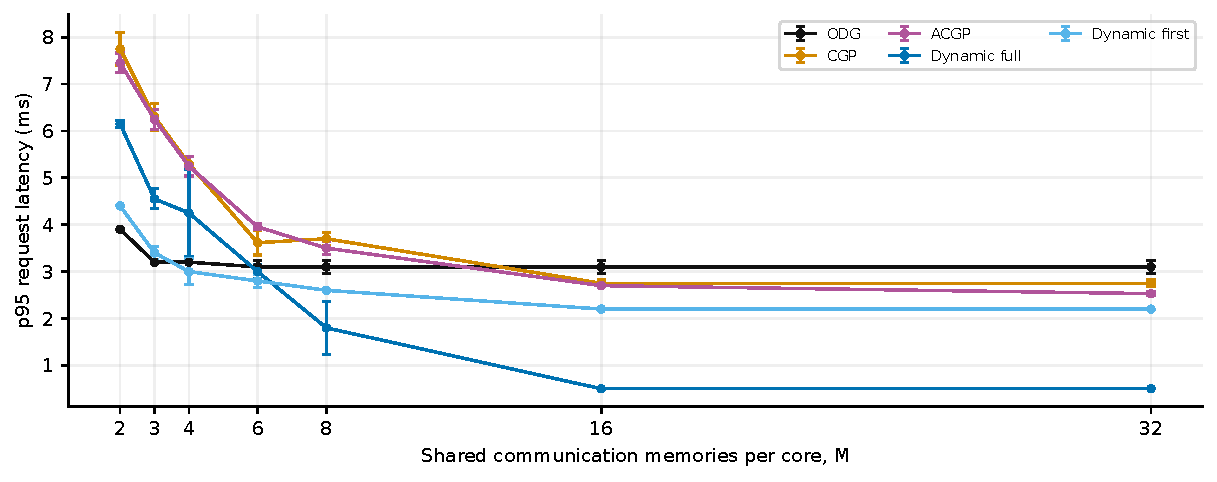
\includegraphics[width=.94\linewidth,height=.255\textheight,keepaspectratio]{figures/memory/mesh_yx_request_latency_p95_ms.pdf}\captionof{figure}{Run-level mean and sample SD. Shared trace aliases are counted once.}\end{center}
\begin{center}{\scriptsize\setlength{\tabcolsep}{3pt}
\begin{tabular}{lrrrrr}
\toprule
M & ODG & CGP & ACGP & Dynamic full & Dynamic first \\
\midrule
2 & $3.900\pm0.000$ & $7.750\pm0.354$ & $7.450\pm0.212$ & $6.150\pm0.071$ & $4.400\pm0.000$ \\
3 & $3.200\pm0.000$ & $6.300\pm0.283$ & $6.250\pm0.212$ & $4.550\pm0.212$ & $3.400\pm0.141$ \\
4 & $3.200\pm0.000$ & $5.300\pm0.000$ & $5.250\pm0.212$ & $4.250\pm0.919$ & $3.000\pm0.283$ \\
6 & $3.100\pm0.141$ & $3.615\pm0.262$ & $3.955\pm0.064$ & $3.000\pm0.141$ & $2.800\pm0.141$ \\
8 & $3.100\pm0.141$ & $3.700\pm0.141$ & $3.500\pm0.141$ & $1.800\pm0.566$ & $2.600\pm0.000$ \\
16 & $3.100\pm0.141$ & $2.750\pm0.071$ & $2.700\pm0.000$ & $0.5000\pm0.0000$ & $2.200\pm0.000$ \\
32 & $3.100\pm0.141$ & $2.750\pm0.071$ & $2.529\pm0.036$ & $0.5000\pm0.0000$ & $2.200\pm0.000$ \\
\bottomrule\end{tabular}}
\captionof{table}{Mean $\pm$ sample SD; n/a denotes a metric outside that policy's instrumentation.}
{\footnotesize\href{https://github.com/sanjeevkrishnaa/Compiler-Driven-ACE/blob/codex/ace-scheduler-correctness/docs/latex/qft96_final/data/memory_mesh_yx_request_latency_p95_ms.csv}{Exact CSV values and sample counts}}
\end{center}
\subsection*{Maximum request latency}
\begin{center}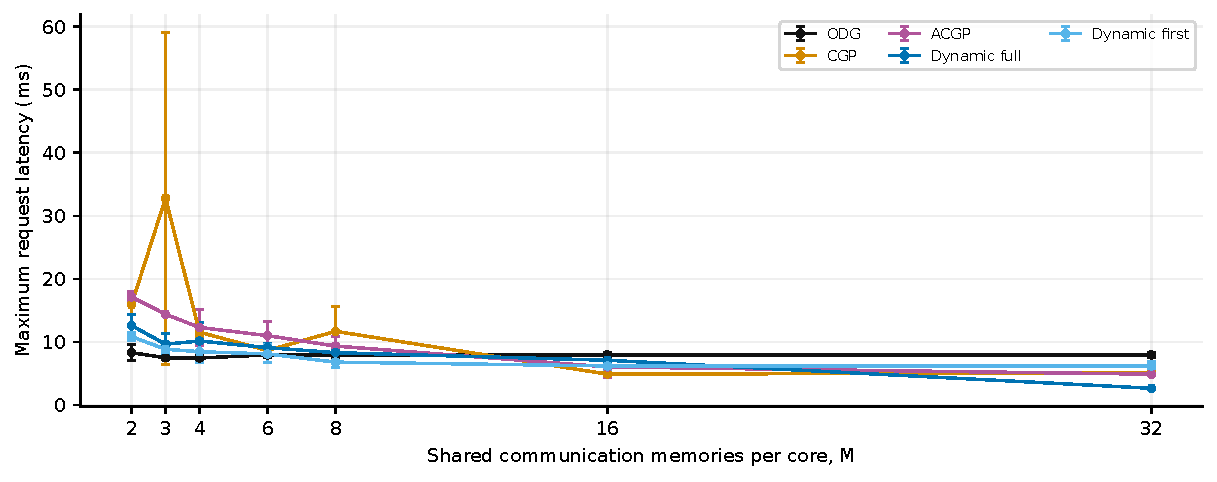
\includegraphics[width=.94\linewidth,height=.255\textheight,keepaspectratio]{figures/memory/mesh_yx_request_latency_max_ms.pdf}\captionof{figure}{Run-level mean and sample SD. Shared trace aliases are counted once.}\end{center}
\begin{center}{\scriptsize\setlength{\tabcolsep}{3pt}
\begin{tabular}{lrrrrr}
\toprule
M & ODG & CGP & ACGP & Dynamic full & Dynamic first \\
\midrule
2 & $8.300\pm1.273$ & $15.900\pm1.556$ & $17.150\pm0.778$ & $12.600\pm1.697$ & $10.850\pm0.636$ \\
3 & $7.500\pm0.283$ & $32.800\pm26.304$ & $14.400\pm0.141$ & $9.650\pm1.626$ & $8.850\pm0.495$ \\
4 & $7.450\pm0.354$ & $11.550\pm0.636$ & $12.300\pm2.828$ & $10.150\pm2.899$ & $8.450\pm1.626$ \\
6 & $7.950\pm0.354$ & $8.650\pm0.778$ & $11.000\pm2.263$ & $9.100\pm0.707$ & $8.100\pm1.414$ \\
8 & $7.950\pm0.354$ & $11.682\pm3.986$ & $9.350\pm1.485$ & $8.300\pm0.283$ & $6.800\pm0.849$ \\
16 & $7.950\pm0.354$ & $4.900\pm0.000$ & $6.043\pm1.616$ & $7.100\pm0.566$ & $6.200\pm0.707$ \\
32 & $7.950\pm0.354$ & $5.096\pm0.277$ & $4.889\pm0.016$ & $2.650\pm0.071$ & $6.200\pm0.707$ \\
\bottomrule\end{tabular}}
\captionof{table}{Mean $\pm$ sample SD; n/a denotes a metric outside that policy's instrumentation.}
{\footnotesize\href{https://github.com/sanjeevkrishnaa/Compiler-Driven-ACE/blob/codex/ace-scheduler-correctness/docs/latex/qft96_final/data/memory_mesh_yx_request_latency_max_ms.csv}{Exact CSV values and sample counts}}
\end{center}
\clearpage
\subsection*{Communication makespan}
\begin{center}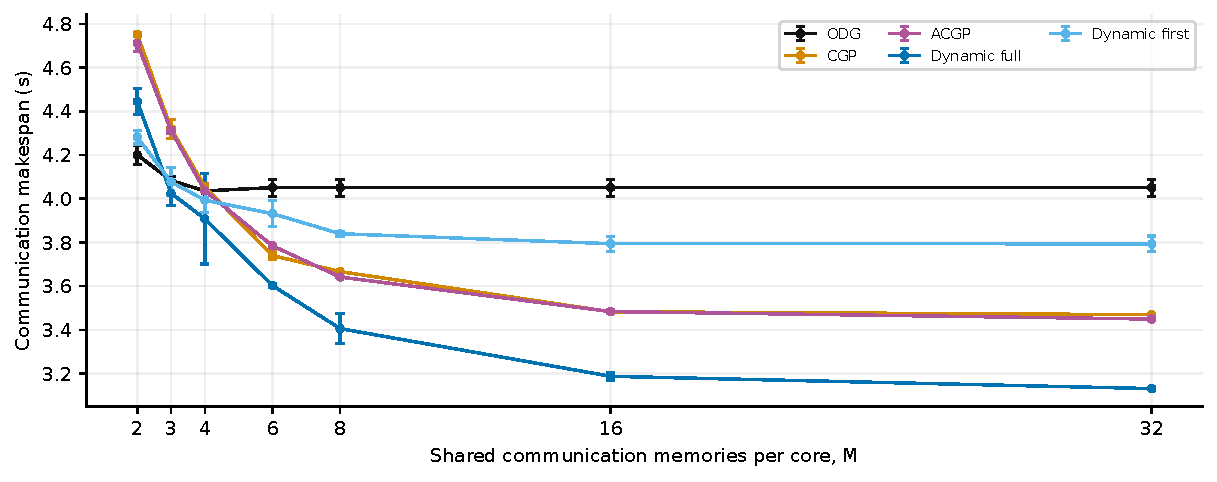
\includegraphics[width=.94\linewidth,height=.255\textheight,keepaspectratio]{figures/memory/mesh_yx_end_to_end_latency_ms.pdf}\captionof{figure}{Run-level mean and sample SD. Shared trace aliases are counted once.}\end{center}
\begin{center}{\scriptsize\setlength{\tabcolsep}{3pt}
\begin{tabular}{lrrrrr}
\toprule
M & ODG & CGP & ACGP & Dynamic full & Dynamic first \\
\midrule
2 & $4.201\pm0.044$ & $4.752\pm0.009$ & $4.711\pm0.036$ & $4.445\pm0.058$ & $4.282\pm0.032$ \\
3 & $4.083\pm0.017$ & $4.321\pm0.044$ & $4.312\pm0.013$ & $4.025\pm0.055$ & $4.077\pm0.064$ \\
4 & $4.036\pm0.032$ & $4.055\pm0.006$ & $4.037\pm0.032$ & $3.908\pm0.207$ & $3.993\pm0.058$ \\
6 & $4.051\pm0.039$ & $3.740\pm0.018$ & $3.784\pm0.006$ & $3.603\pm0.008$ & $3.932\pm0.060$ \\
8 & $4.051\pm0.039$ & $3.666\pm0.002$ & $3.642\pm0.004$ & $3.406\pm0.070$ & $3.840\pm0.011$ \\
16 & $4.051\pm0.039$ & $3.483\pm0.001$ & $3.484\pm0.008$ & $3.187\pm0.017$ & $3.794\pm0.035$ \\
32 & $4.051\pm0.039$ & $3.469\pm0.006$ & $3.449\pm0.007$ & $3.131\pm0.001$ & $3.794\pm0.035$ \\
\bottomrule\end{tabular}}
\captionof{table}{Mean $\pm$ sample SD; n/a denotes a metric outside that policy's instrumentation.}
{\footnotesize\href{https://github.com/sanjeevkrishnaa/Compiler-Driven-ACE/blob/codex/ace-scheduler-correctness/docs/latex/qft96_final/data/memory_mesh_yx_end_to_end_latency_ms.csv}{Exact CSV values and sample counts}}
\end{center}
\subsection*{Mean admission wait}
\begin{center}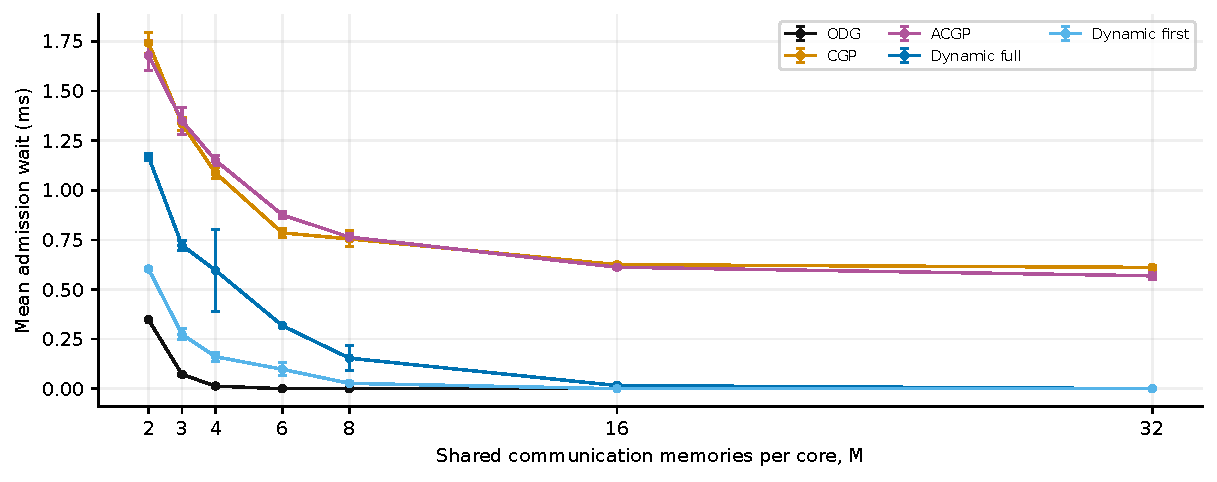
\includegraphics[width=.94\linewidth,height=.255\textheight,keepaspectratio]{figures/memory/mesh_yx_average_admission_wait_ms.pdf}\captionof{figure}{Run-level mean and sample SD. Shared trace aliases are counted once.}\end{center}
\begin{center}{\scriptsize\setlength{\tabcolsep}{3pt}
\begin{tabular}{lrrrrr}
\toprule
M & ODG & CGP & ACGP & Dynamic full & Dynamic first \\
\midrule
2 & $0.3471\pm0.0048$ & $1.742\pm0.054$ & $1.679\pm0.077$ & $1.167\pm0.016$ & $0.6028\pm0.0088$ \\
3 & $0.0722\pm0.0055$ & $1.334\pm0.033$ & $1.349\pm0.069$ & $0.7224\pm0.0258$ & $0.2747\pm0.0290$ \\
4 & $0.0133\pm0.0009$ & $1.087\pm0.029$ & $1.151\pm0.026$ & $0.5966\pm0.2069$ & $0.1613\pm0.0227$ \\
6 & $0.0000\pm0.0000$ & $0.7850\pm0.0223$ & $0.8758\pm0.0180$ & $0.3175\pm0.0065$ & $0.0979\pm0.0325$ \\
8 & $0.0000\pm0.0000$ & $0.7549\pm0.0405$ & $0.7639\pm0.0186$ & $0.1541\pm0.0621$ & $0.0272\pm0.0076$ \\
16 & $0.0000\pm0.0000$ & $0.6250\pm0.0060$ & $0.6123\pm0.0040$ & $0.0160\pm0.0051$ & $0.0001\pm0.0001$ \\
32 & $0.0000\pm0.0000$ & $0.6112\pm0.0119$ & $0.5687\pm0.0190$ & $0.0001\pm0.0002$ & $0.0000\pm0.0000$ \\
\bottomrule\end{tabular}}
\captionof{table}{Mean $\pm$ sample SD; n/a denotes a metric outside that policy's instrumentation.}
{\footnotesize\href{https://github.com/sanjeevkrishnaa/Compiler-Driven-ACE/blob/codex/ace-scheduler-correctness/docs/latex/qft96_final/data/memory_mesh_yx_average_admission_wait_ms.csv}{Exact CSV values and sample counts}}
\end{center}
\clearpage
\subsection*{Delivered EPR fidelity}
\begin{center}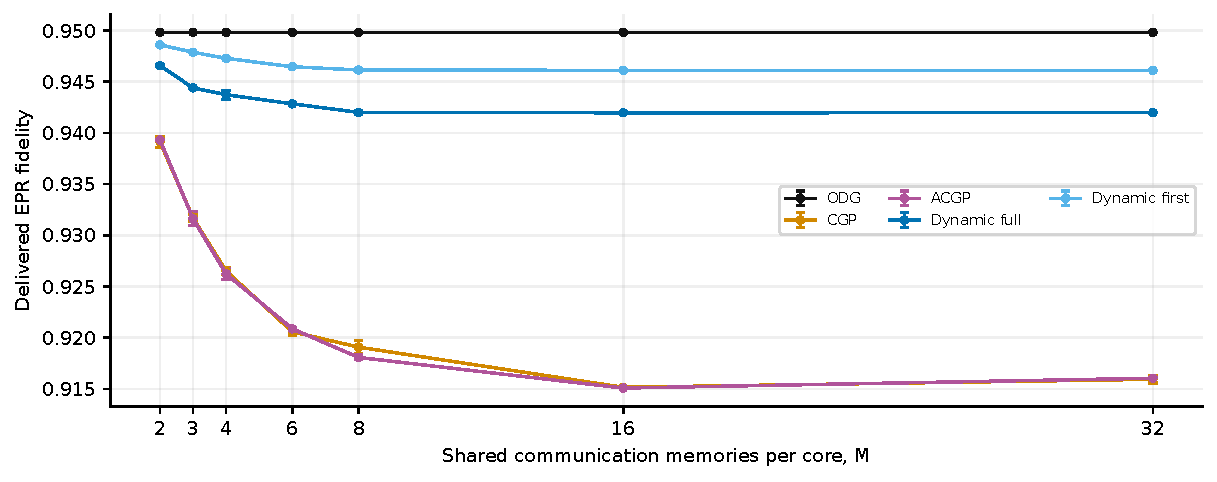
\includegraphics[width=.94\linewidth,height=.255\textheight,keepaspectratio]{figures/memory/mesh_yx_average_delivered_epr_fidelity.pdf}\captionof{figure}{Run-level mean and sample SD. Shared trace aliases are counted once.}\end{center}
\begin{center}{\scriptsize\setlength{\tabcolsep}{3pt}
\begin{tabular}{lrrrrr}
\toprule
M & ODG & CGP & ACGP & Dynamic full & Dynamic first \\
\midrule
2 & $0.9498\pm0.0000$ & $0.9391\pm0.0005$ & $0.9393\pm0.0000$ & $0.9466\pm0.0001$ & $0.9486\pm0.0000$ \\
3 & $0.9498\pm0.0000$ & $0.9317\pm0.0003$ & $0.9316\pm0.0007$ & $0.9444\pm0.0001$ & $0.9479\pm0.0000$ \\
4 & $0.9498\pm0.0000$ & $0.9265\pm0.0003$ & $0.9262\pm0.0006$ & $0.9437\pm0.0004$ & $0.9473\pm0.0000$ \\
6 & $0.9498\pm0.0000$ & $0.9206\pm0.0003$ & $0.9209\pm0.0001$ & $0.9428\pm0.0000$ & $0.9465\pm0.0001$ \\
8 & $0.9498\pm0.0000$ & $0.9191\pm0.0006$ & $0.9181\pm0.0002$ & $0.9420\pm0.0002$ & $0.9461\pm0.0000$ \\
16 & $0.9498\pm0.0000$ & $0.9152\pm0.0000$ & $0.9151\pm0.0001$ & $0.9420\pm0.0000$ & $0.9461\pm0.0000$ \\
32 & $0.9498\pm0.0000$ & $0.9159\pm0.0004$ & $0.9160\pm0.0000$ & $0.9420\pm0.0000$ & $0.9461\pm0.0000$ \\
\bottomrule\end{tabular}}
\captionof{table}{Mean $\pm$ sample SD; n/a denotes a metric outside that policy's instrumentation.}
{\footnotesize\href{https://github.com/sanjeevkrishnaa/Compiler-Driven-ACE/blob/codex/ace-scheduler-correctness/docs/latex/qft96_final/data/memory_mesh_yx_average_delivered_epr_fidelity.csv}{Exact CSV values and sample counts}}
\end{center}
\subsection*{Compiler readiness fraction}
\begin{center}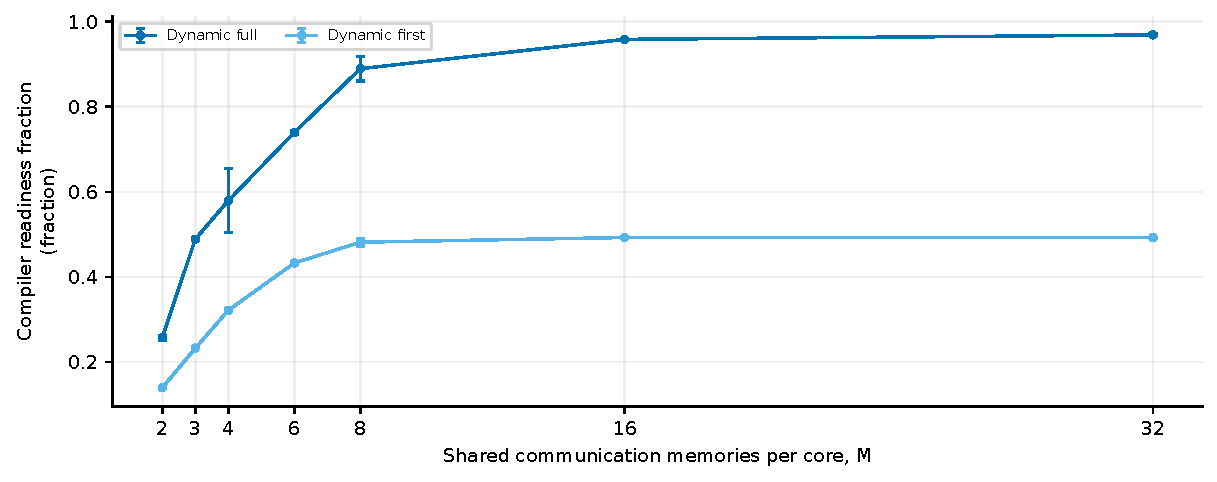
\includegraphics[width=.94\linewidth,height=.255\textheight,keepaspectratio]{figures/memory/mesh_yx_pregenerated_success_rate.pdf}\captionof{figure}{Run-level mean and sample SD. Shared trace aliases are counted once.}\end{center}
\begin{center}{\scriptsize\setlength{\tabcolsep}{3pt}
\begin{tabular}{lrrrrr}
\toprule
M & ODG & CGP & ACGP & Dynamic full & Dynamic first \\
\midrule
2 & n/a & n/a & n/a & $0.2571\pm0.0060$ & $0.1398\pm0.0026$ \\
3 & n/a & n/a & n/a & $0.4889\pm0.0004$ & $0.2328\pm0.0005$ \\
4 & n/a & n/a & n/a & $0.5795\pm0.0752$ & $0.3219\pm0.0020$ \\
6 & n/a & n/a & n/a & $0.7397\pm0.0044$ & $0.4329\pm0.0044$ \\
8 & n/a & n/a & n/a & $0.8894\pm0.0290$ & $0.4818\pm0.0097$ \\
16 & n/a & n/a & n/a & $0.9583\pm0.0027$ & $0.4928\pm0.0011$ \\
32 & n/a & n/a & n/a & $0.9688\pm0.0022$ & $0.4928\pm0.0011$ \\
\bottomrule\end{tabular}}
\captionof{table}{Mean $\pm$ sample SD; n/a denotes a metric outside that policy's instrumentation.}
{\footnotesize\href{https://github.com/sanjeevkrishnaa/Compiler-Driven-ACE/blob/codex/ace-scheduler-correctness/docs/latex/qft96_final/data/memory_mesh_yx_pregenerated_success_rate.csv}{Exact CSV values and sample counts}}
\end{center}
\clearpage
\subsection*{Intended compiler-hit fraction}
\begin{center}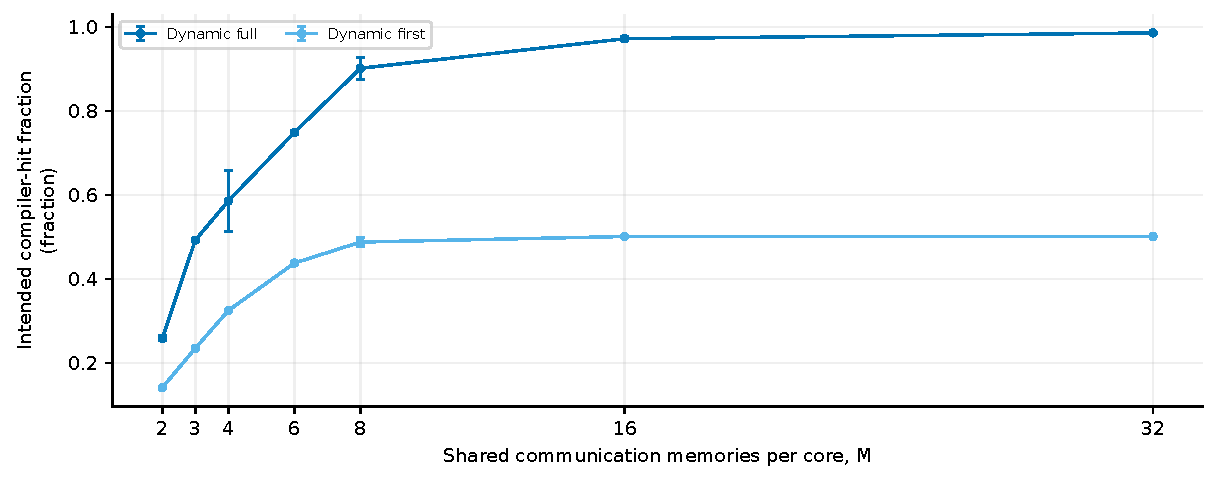
\includegraphics[width=.94\linewidth,height=.255\textheight,keepaspectratio]{figures/memory/mesh_yx_intended_request_hit_rate.pdf}\captionof{figure}{Run-level mean and sample SD. Shared trace aliases are counted once.}\end{center}
\begin{center}{\scriptsize\setlength{\tabcolsep}{3pt}
\begin{tabular}{lrrrrr}
\toprule
M & ODG & CGP & ACGP & Dynamic full & Dynamic first \\
\midrule
2 & n/a & n/a & n/a & $0.2585\pm0.0062$ & $0.1409\pm0.0026$ \\
3 & n/a & n/a & n/a & $0.4923\pm0.0015$ & $0.2346\pm0.0013$ \\
4 & n/a & n/a & n/a & $0.5857\pm0.0733$ & $0.3246\pm0.0007$ \\
6 & n/a & n/a & n/a & $0.7488\pm0.0042$ & $0.4377\pm0.0042$ \\
8 & n/a & n/a & n/a & $0.9017\pm0.0255$ & $0.4877\pm0.0104$ \\
16 & n/a & n/a & n/a & $0.9721\pm0.0044$ & $0.5010\pm0.0011$ \\
32 & n/a & n/a & n/a & $0.9862\pm0.0013$ & $0.5010\pm0.0011$ \\
\bottomrule\end{tabular}}
\captionof{table}{Mean $\pm$ sample SD; n/a denotes a metric outside that policy's instrumentation.}
{\footnotesize\href{https://github.com/sanjeevkrishnaa/Compiler-Driven-ACE/blob/codex/ace-scheduler-correctness/docs/latex/qft96_final/data/memory_mesh_yx_intended_request_hit_rate.csv}{Exact CSV values and sample counts}}
\end{center}
\subsection*{Compiler fallback fraction}
\begin{center}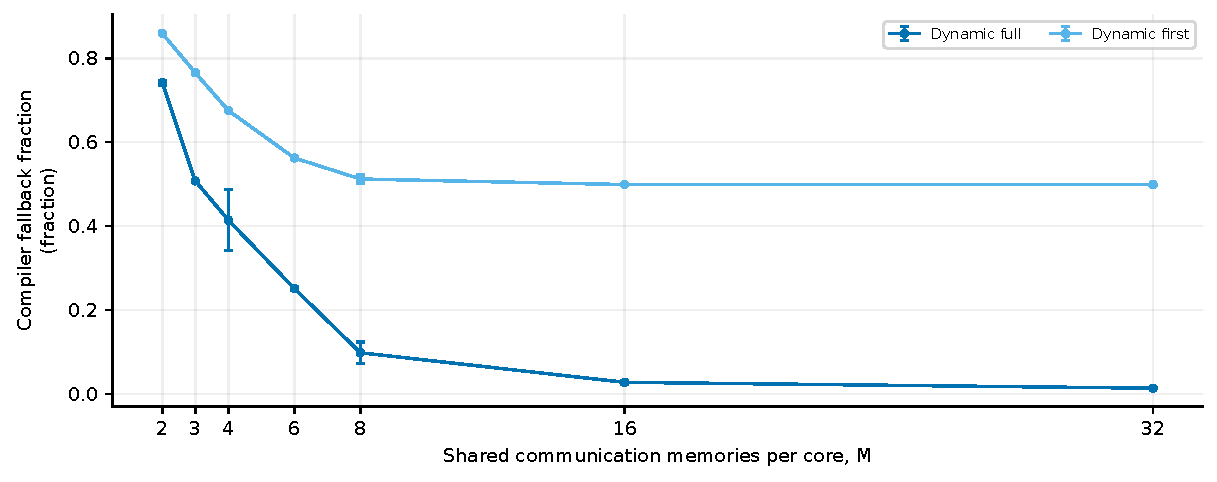
\includegraphics[width=.94\linewidth,height=.255\textheight,keepaspectratio]{figures/memory/mesh_yx_on_demand_fallback_rate.pdf}\captionof{figure}{Run-level mean and sample SD. Shared trace aliases are counted once.}\end{center}
\begin{center}{\scriptsize\setlength{\tabcolsep}{3pt}
\begin{tabular}{lrrrrr}
\toprule
M & ODG & CGP & ACGP & Dynamic full & Dynamic first \\
\midrule
2 & n/a & n/a & n/a & $0.7415\pm0.0062$ & $0.8591\pm0.0026$ \\
3 & n/a & n/a & n/a & $0.5077\pm0.0015$ & $0.7654\pm0.0013$ \\
4 & n/a & n/a & n/a & $0.4143\pm0.0733$ & $0.6754\pm0.0007$ \\
6 & n/a & n/a & n/a & $0.2512\pm0.0042$ & $0.5623\pm0.0042$ \\
8 & n/a & n/a & n/a & $0.0983\pm0.0255$ & $0.5123\pm0.0104$ \\
16 & n/a & n/a & n/a & $0.0279\pm0.0044$ & $0.4990\pm0.0011$ \\
32 & n/a & n/a & n/a & $0.0138\pm0.0013$ & $0.4990\pm0.0011$ \\
\bottomrule\end{tabular}}
\captionof{table}{Mean $\pm$ sample SD; n/a denotes a metric outside that policy's instrumentation.}
{\footnotesize\href{https://github.com/sanjeevkrishnaa/Compiler-Driven-ACE/blob/codex/ace-scheduler-correctness/docs/latex/qft96_final/data/memory_mesh_yx_on_demand_fallback_rate.csv}{Exact CSV values and sample counts}}
\end{center}
\clearpage
\subsection*{Compiler-cache waste}
\begin{center}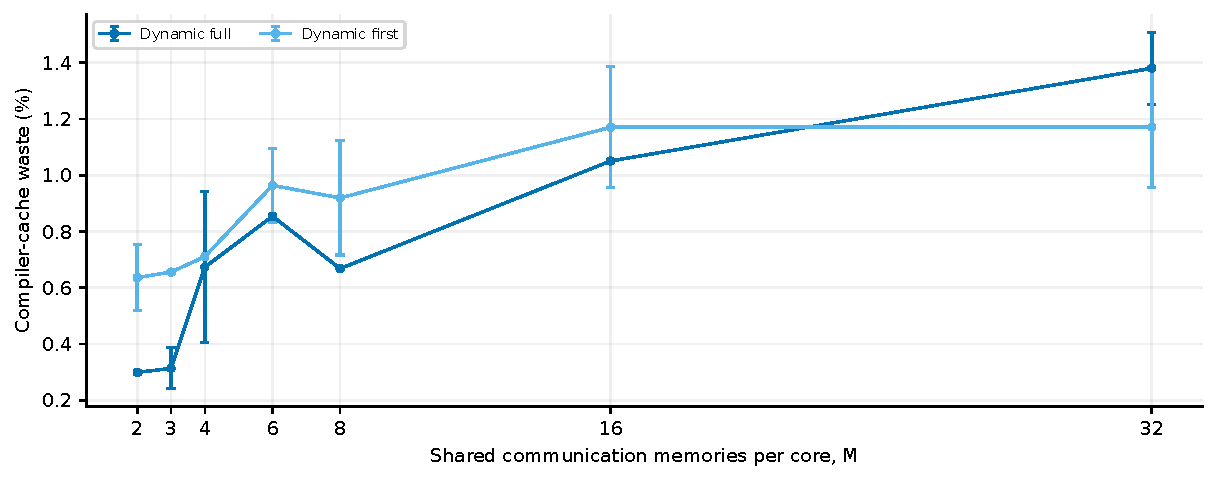
\includegraphics[width=.94\linewidth,height=.255\textheight,keepaspectratio]{figures/memory/mesh_yx_compiler_waste_percentage.pdf}\captionof{figure}{Run-level mean and sample SD. Shared trace aliases are counted once.}\end{center}
\begin{center}{\scriptsize\setlength{\tabcolsep}{3pt}
\begin{tabular}{lrrrrr}
\toprule
M & ODG & CGP & ACGP & Dynamic full & Dynamic first \\
\midrule
2 & n/a & n/a & n/a & $0.2986\pm0.0071$ & $0.6358\pm0.1164$ \\
3 & n/a & n/a & n/a & $0.3133\pm0.0727$ & $0.6554\pm0.0035$ \\
4 & n/a & n/a & n/a & $0.6729\pm0.2681$ & $0.7103\pm0.0016$ \\
6 & n/a & n/a & n/a & $0.8540\pm0.0047$ & $0.9638\pm0.1318$ \\
8 & n/a & n/a & n/a & $0.6679\pm0.0012$ & $0.9191\pm0.2030$ \\
16 & n/a & n/a & n/a & $1.050\pm0.005$ & $1.170\pm0.216$ \\
32 & n/a & n/a & n/a & $1.380\pm0.128$ & $1.170\pm0.216$ \\
\bottomrule\end{tabular}}
\captionof{table}{Mean $\pm$ sample SD; n/a denotes a metric outside that policy's instrumentation.}
{\footnotesize\href{https://github.com/sanjeevkrishnaa/Compiler-Driven-ACE/blob/codex/ace-scheduler-correctness/docs/latex/qft96_final/data/memory_mesh_yx_compiler_waste_percentage.csv}{Exact CSV values and sample counts}}
\end{center}
\subsection*{Native-protocol waste}
\begin{center}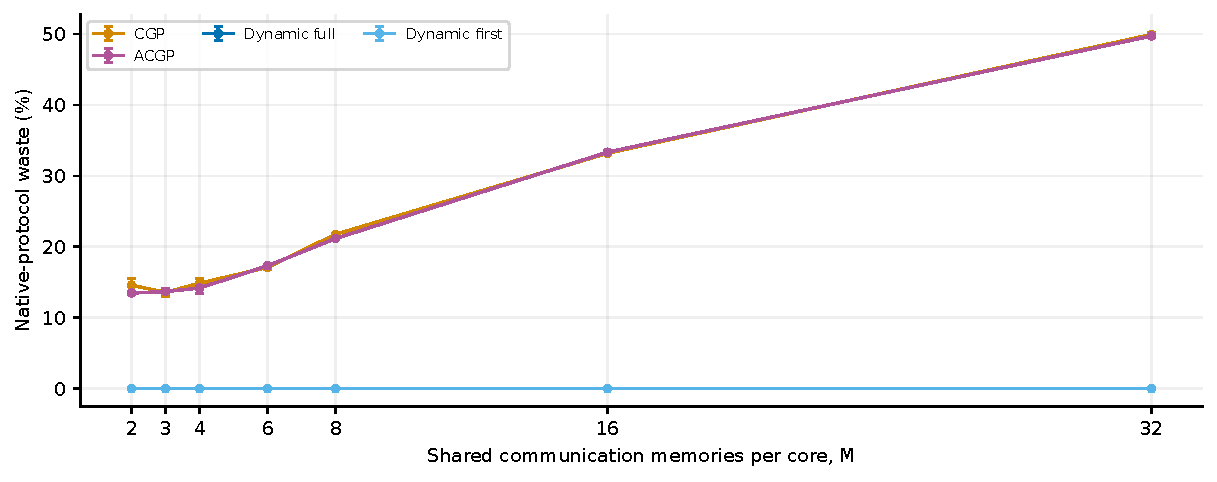
\includegraphics[width=.94\linewidth,height=.255\textheight,keepaspectratio]{figures/memory/mesh_yx_protocol_waste_percentage.pdf}\captionof{figure}{Run-level mean and sample SD. Shared trace aliases are counted once.}\end{center}
\begin{center}{\scriptsize\setlength{\tabcolsep}{3pt}
\begin{tabular}{lrrrrr}
\toprule
M & ODG & CGP & ACGP & Dynamic full & Dynamic first \\
\midrule
2 & n/a & $14.584\pm0.965$ & $13.483\pm0.264$ & $0.0000\pm0.0000$ & $0.0000\pm0.0000$ \\
3 & n/a & $13.576\pm0.514$ & $13.689\pm0.374$ & $0.0000\pm0.0000$ & $0.0000\pm0.0000$ \\
4 & n/a & $14.863\pm0.627$ & $14.186\pm0.779$ & $0.0000\pm0.0000$ & $0.0000\pm0.0000$ \\
6 & n/a & $17.093\pm0.215$ & $17.325\pm0.096$ & $0.0000\pm0.0000$ & $0.0000\pm0.0000$ \\
8 & n/a & $21.758\pm0.013$ & $21.168\pm0.053$ & $0.0000\pm0.0000$ & $0.0000\pm0.0000$ \\
16 & n/a & $33.183\pm0.156$ & $33.336\pm0.069$ & $0.0000\pm0.0000$ & $0.0000\pm0.0000$ \\
32 & n/a & $49.910\pm0.312$ & $49.715\pm0.211$ & $0.0000\pm0.0000$ & $0.0000\pm0.0000$ \\
\bottomrule\end{tabular}}
\captionof{table}{Mean $\pm$ sample SD; n/a denotes a metric outside that policy's instrumentation.}
{\footnotesize\href{https://github.com/sanjeevkrishnaa/Compiler-Driven-ACE/blob/codex/ace-scheduler-correctness/docs/latex/qft96_final/data/memory_mesh_yx_protocol_waste_percentage.csv}{Exact CSV values and sample counts}}
\end{center}
\clearpage
\subsection*{Compiler-pair expiry}
\begin{center}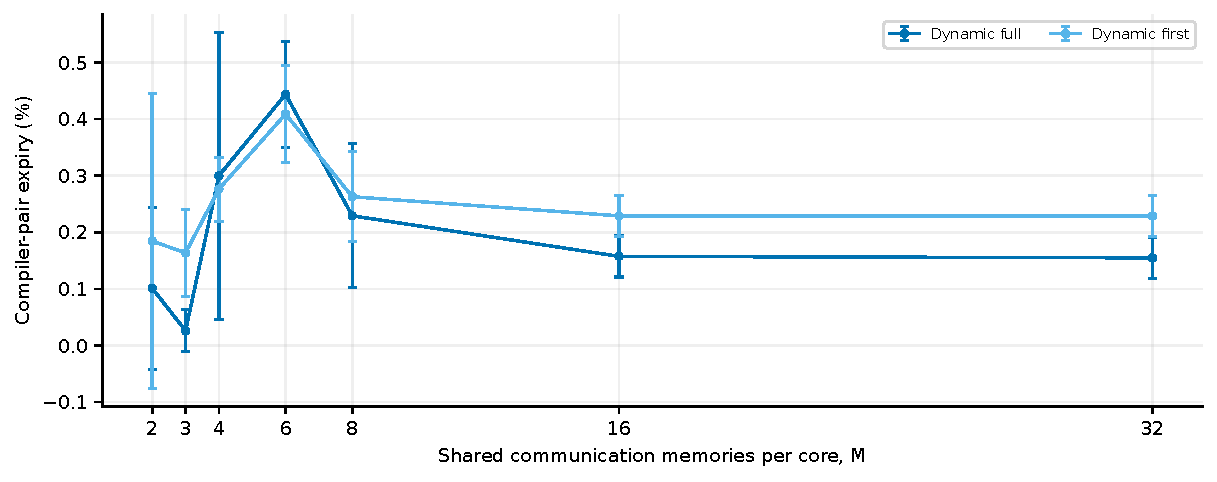
\includegraphics[width=.94\linewidth,height=.255\textheight,keepaspectratio]{figures/memory/mesh_yx_compiler_expiry_percentage.pdf}\captionof{figure}{Run-level mean and sample SD. Shared trace aliases are counted once.}\end{center}
\begin{center}{\scriptsize\setlength{\tabcolsep}{3pt}
\begin{tabular}{lrrrrr}
\toprule
M & ODG & CGP & ACGP & Dynamic full & Dynamic first \\
\midrule
2 & n/a & n/a & n/a & $0.1012\pm0.1431$ & $0.1845\pm0.2609$ \\
3 & n/a & n/a & n/a & $0.0261\pm0.0368$ & $0.1636\pm0.0764$ \\
4 & n/a & n/a & n/a & $0.3000\pm0.2534$ & $0.2763\pm0.0564$ \\
6 & n/a & n/a & n/a & $0.4438\pm0.0942$ & $0.4090\pm0.0859$ \\
8 & n/a & n/a & n/a & $0.2292\pm0.1271$ & $0.2628\pm0.0792$ \\
16 & n/a & n/a & n/a & $0.1575\pm0.0364$ & $0.2290\pm0.0360$ \\
32 & n/a & n/a & n/a & $0.1548\pm0.0365$ & $0.2290\pm0.0360$ \\
\bottomrule\end{tabular}}
\captionof{table}{Mean $\pm$ sample SD; n/a denotes a metric outside that policy's instrumentation.}
{\footnotesize\href{https://github.com/sanjeevkrishnaa/Compiler-Driven-ACE/blob/codex/ace-scheduler-correctness/docs/latex/qft96_final/data/memory_mesh_yx_compiler_expiry_percentage.csv}{Exact CSV values and sample counts}}
\end{center}
\subsection*{Used compiler-pair storage time}
\begin{center}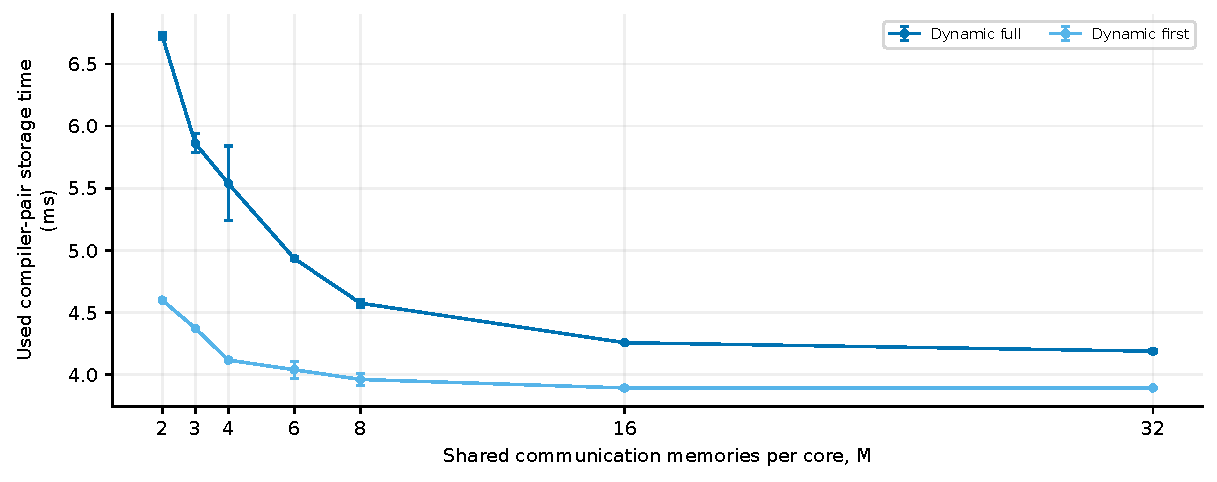
\includegraphics[width=.94\linewidth,height=.255\textheight,keepaspectratio]{figures/memory/mesh_yx_average_storage_time_ms.pdf}\captionof{figure}{Run-level mean and sample SD. Shared trace aliases are counted once.}\end{center}
\begin{center}{\scriptsize\setlength{\tabcolsep}{3pt}
\begin{tabular}{lrrrrr}
\toprule
M & ODG & CGP & ACGP & Dynamic full & Dynamic first \\
\midrule
2 & n/a & n/a & n/a & $6.726\pm0.029$ & $4.600\pm0.012$ \\
3 & n/a & n/a & n/a & $5.862\pm0.078$ & $4.374\pm0.004$ \\
4 & n/a & n/a & n/a & $5.539\pm0.301$ & $4.118\pm0.008$ \\
6 & n/a & n/a & n/a & $4.935\pm0.013$ & $4.040\pm0.067$ \\
8 & n/a & n/a & n/a & $4.576\pm0.031$ & $3.962\pm0.045$ \\
16 & n/a & n/a & n/a & $4.258\pm0.004$ & $3.894\pm0.006$ \\
32 & n/a & n/a & n/a & $4.189\pm0.010$ & $3.894\pm0.006$ \\
\bottomrule\end{tabular}}
\captionof{table}{Mean $\pm$ sample SD; n/a denotes a metric outside that policy's instrumentation.}
{\footnotesize\href{https://github.com/sanjeevkrishnaa/Compiler-Driven-ACE/blob/codex/ace-scheduler-correctness/docs/latex/qft96_final/data/memory_mesh_yx_average_storage_time_ms.csv}{Exact CSV values and sample counts}}
\end{center}
\clearpage
\subsection*{Delivered-hop throughput}
\begin{center}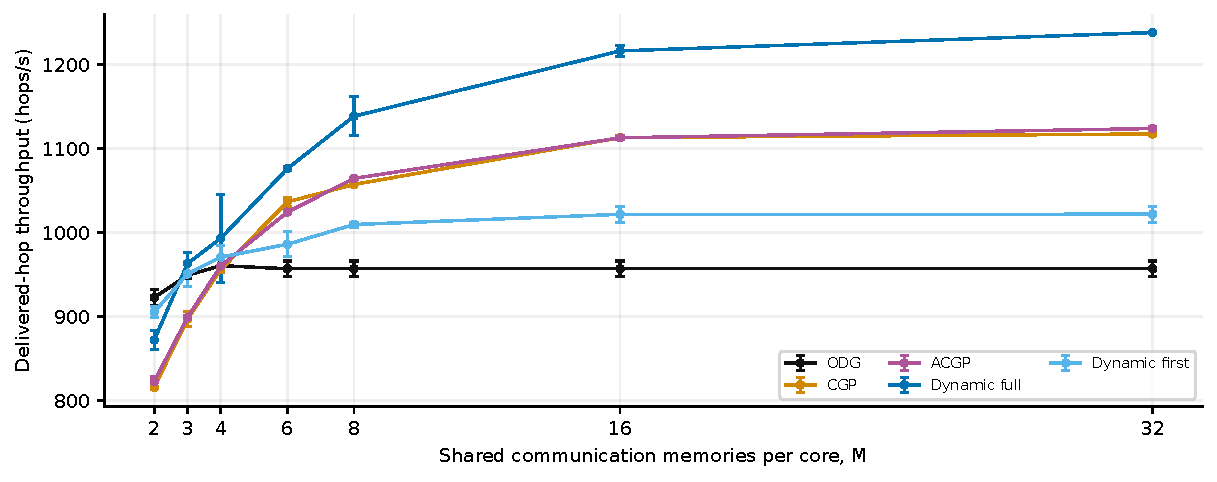
\includegraphics[width=.94\linewidth,height=.255\textheight,keepaspectratio]{figures/memory/mesh_yx_hop_throughput_s.pdf}\captionof{figure}{Run-level mean and sample SD. Shared trace aliases are counted once.}\end{center}
\begin{center}{\scriptsize\setlength{\tabcolsep}{3pt}
\begin{tabular}{lrrrrr}
\toprule
M & ODG & CGP & ACGP & Dynamic full & Dynamic first \\
\midrule
2 & $922.64\pm9.60$ & $815.59\pm1.56$ & $822.74\pm6.27$ & $872.09\pm11.45$ & $905.17\pm6.74$ \\
3 & $949.24\pm4.06$ & $897.11\pm9.06$ & $898.90\pm2.79$ & $962.99\pm13.06$ & $950.73\pm15.02$ \\
4 & $960.49\pm7.66$ & $955.82\pm1.48$ & $960.24\pm7.66$ & $993.15\pm52.58$ & $970.68\pm14.08$ \\
6 & $956.85\pm9.24$ & $1036.39\pm5.06$ & $1024.22\pm1.73$ & $1075.89\pm2.53$ & $985.97\pm15.04$ \\
8 & $956.85\pm9.24$ & $1057.15\pm0.59$ & $1064.32\pm1.21$ & $1138.33\pm23.35$ & $1009.43\pm2.90$ \\
16 & $956.85\pm9.24$ & $1112.88\pm0.48$ & $1112.65\pm2.46$ & $1216.05\pm6.42$ & $1021.60\pm9.41$ \\
32 & $956.85\pm9.24$ & $1117.24\pm2.01$ & $1123.71\pm2.26$ & $1237.92\pm0.25$ & $1021.71\pm9.56$ \\
\bottomrule\end{tabular}}
\captionof{table}{Mean $\pm$ sample SD; n/a denotes a metric outside that policy's instrumentation.}
{\footnotesize\href{https://github.com/sanjeevkrishnaa/Compiler-Driven-ACE/blob/codex/ace-scheduler-correctness/docs/latex/qft96_final/data/memory_mesh_yx_hop_throughput_s.csv}{Exact CSV values and sample counts}}
\end{center}
\subsection*{Completion fraction}
\begin{center}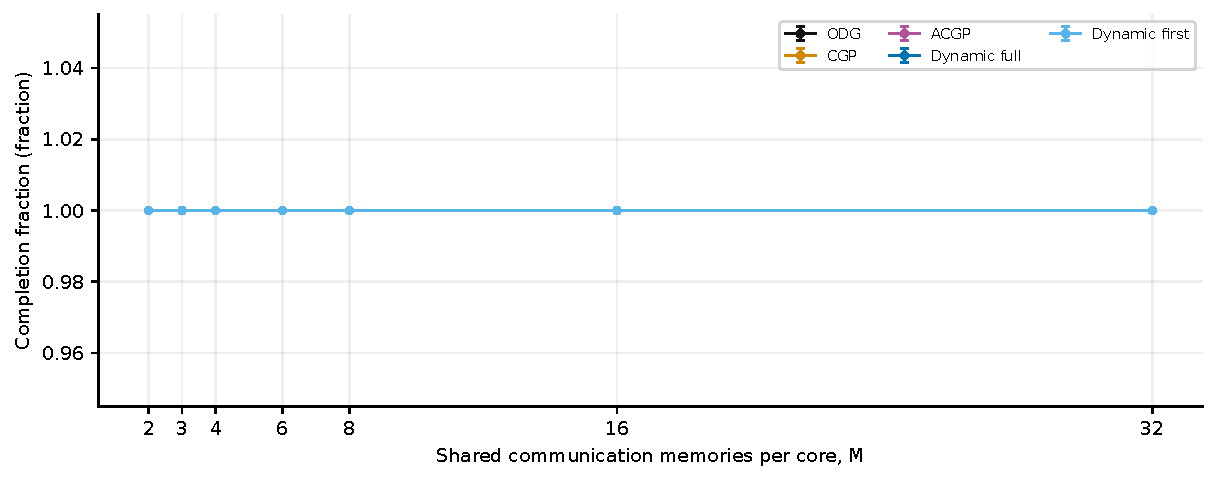
\includegraphics[width=.94\linewidth,height=.255\textheight,keepaspectratio]{figures/memory/mesh_yx_completion_rate.pdf}\captionof{figure}{Run-level mean and sample SD. Shared trace aliases are counted once.}\end{center}
\begin{center}{\scriptsize\setlength{\tabcolsep}{3pt}
\begin{tabular}{lrrrrr}
\toprule
M & ODG & CGP & ACGP & Dynamic full & Dynamic first \\
\midrule
2 & $1.000\pm0.000$ & $1.000\pm0.000$ & $1.000\pm0.000$ & $1.000\pm0.000$ & $1.000\pm0.000$ \\
3 & $1.000\pm0.000$ & $1.000\pm0.000$ & $1.000\pm0.000$ & $1.000\pm0.000$ & $1.000\pm0.000$ \\
4 & $1.000\pm0.000$ & $1.000\pm0.000$ & $1.000\pm0.000$ & $1.000\pm0.000$ & $1.000\pm0.000$ \\
6 & $1.000\pm0.000$ & $1.000\pm0.000$ & $1.000\pm0.000$ & $1.000\pm0.000$ & $1.000\pm0.000$ \\
8 & $1.000\pm0.000$ & $1.000\pm0.000$ & $1.000\pm0.000$ & $1.000\pm0.000$ & $1.000\pm0.000$ \\
16 & $1.000\pm0.000$ & $1.000\pm0.000$ & $1.000\pm0.000$ & $1.000\pm0.000$ & $1.000\pm0.000$ \\
32 & $1.000\pm0.000$ & $1.000\pm0.000$ & $1.000\pm0.000$ & $1.000\pm0.000$ & $1.000\pm0.000$ \\
\bottomrule\end{tabular}}
\captionof{table}{Mean $\pm$ sample SD; n/a denotes a metric outside that policy's instrumentation.}
{\footnotesize\href{https://github.com/sanjeevkrishnaa/Compiler-Driven-ACE/blob/codex/ace-scheduler-correctness/docs/latex/qft96_final/data/memory_mesh_yx_completion_rate.csv}{Exact CSV values and sample counts}}
\end{center}
\clearpage
\subsection*{Maximum admission wait}
\begin{center}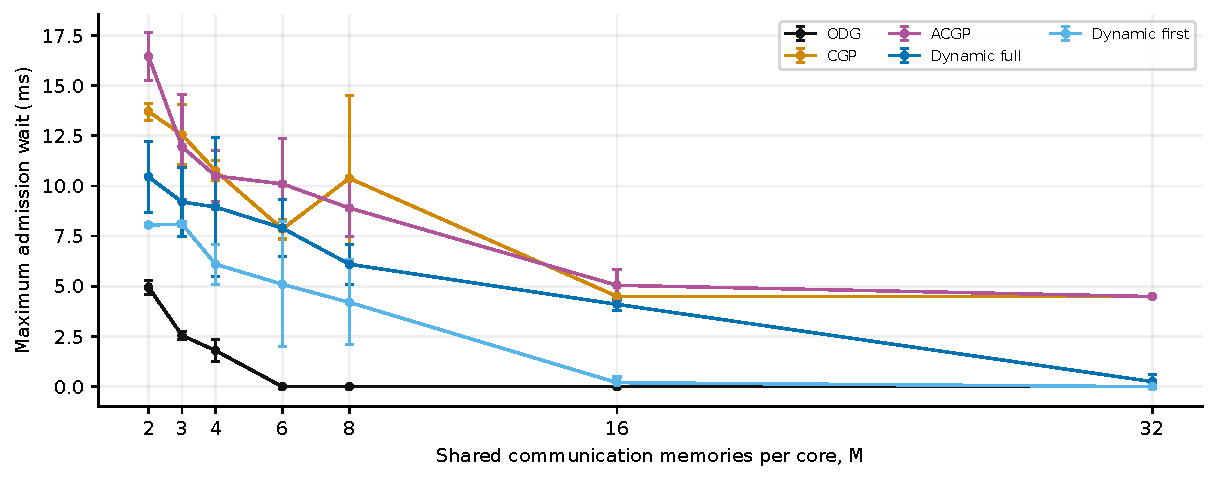
\includegraphics[width=.94\linewidth,height=.255\textheight,keepaspectratio]{figures/memory/mesh_yx_max_admission_wait_ms.pdf}\captionof{figure}{Run-level mean and sample SD. Shared trace aliases are counted once.}\end{center}
\begin{center}{\scriptsize\setlength{\tabcolsep}{3pt}
\begin{tabular}{lrrrrr}
\toprule
M & ODG & CGP & ACGP & Dynamic full & Dynamic first \\
\midrule
2 & $4.950\pm0.354$ & $13.700\pm0.424$ & $16.450\pm1.202$ & $10.450\pm1.768$ & $8.050\pm0.071$ \\
3 & $2.550\pm0.212$ & $12.550\pm1.485$ & $11.950\pm2.616$ & $9.200\pm1.697$ & $8.100\pm0.141$ \\
4 & $1.800\pm0.566$ & $10.752\pm0.497$ & $10.500\pm1.273$ & $8.950\pm3.465$ & $6.100\pm0.990$ \\
6 & $0.0000\pm0.0000$ & $7.850\pm0.495$ & $10.100\pm2.263$ & $7.900\pm1.414$ & $5.100\pm3.111$ \\
8 & $0.0000\pm0.0000$ & $10.382\pm4.127$ & $8.900\pm1.414$ & $6.100\pm0.990$ & $4.200\pm2.121$ \\
16 & $0.0000\pm0.0000$ & $4.500\pm0.000$ & $5.050\pm0.778$ & $4.100\pm0.283$ & $0.2000\pm0.2828$ \\
32 & $0.0000\pm0.0000$ & $4.500\pm0.000$ & $4.489\pm0.016$ & $0.2500\pm0.3536$ & $0.0000\pm0.0000$ \\
\bottomrule\end{tabular}}
\captionof{table}{Mean $\pm$ sample SD; n/a denotes a metric outside that policy's instrumentation.}
{\footnotesize\href{https://github.com/sanjeevkrishnaa/Compiler-Driven-ACE/blob/codex/ace-scheduler-correctness/docs/latex/qft96_final/data/memory_mesh_yx_max_admission_wait_ms.csv}{Exact CSV values and sample counts}}
\end{center}
\subsection*{Requests with admission wait}
\begin{center}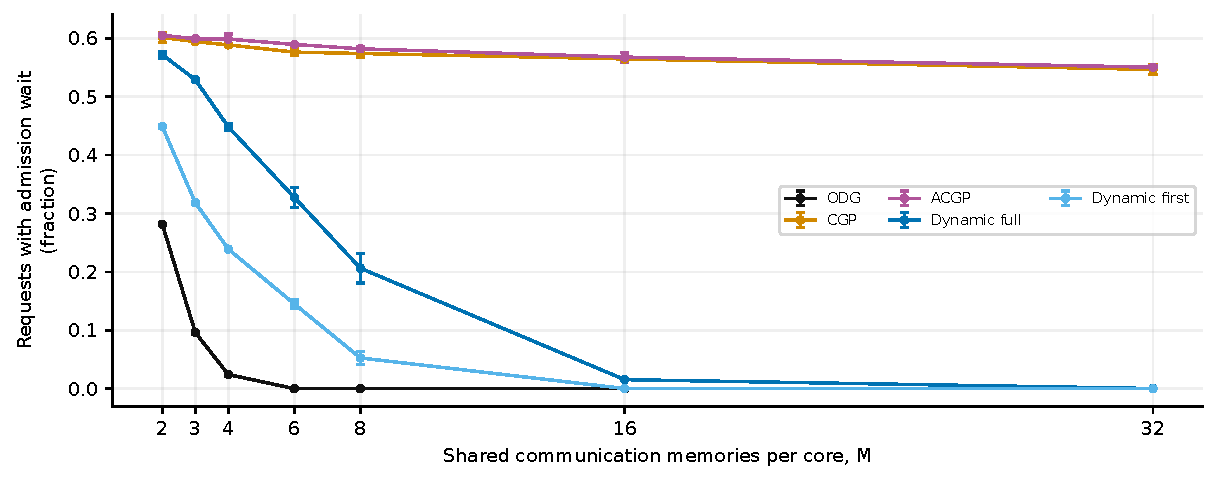
\includegraphics[width=.94\linewidth,height=.255\textheight,keepaspectratio]{figures/memory/mesh_yx_requests_that_waited_fraction.pdf}\captionof{figure}{Run-level mean and sample SD. Shared trace aliases are counted once.}\end{center}
\begin{center}{\scriptsize\setlength{\tabcolsep}{3pt}
\begin{tabular}{lrrrrr}
\toprule
M & ODG & CGP & ACGP & Dynamic full & Dynamic first \\
\midrule
2 & $0.2816\pm0.0009$ & $0.6014\pm0.0088$ & $0.6050\pm0.0018$ & $0.5719\pm0.0057$ & $0.4489\pm0.0018$ \\
3 & $0.0962\pm0.0022$ & $0.5942\pm0.0011$ & $0.5992\pm0.0027$ & $0.5290\pm0.0005$ & $0.3185\pm0.0024$ \\
4 & $0.0243\pm0.0000$ & $0.5886\pm0.0024$ & $0.5986\pm0.0088$ & $0.4483\pm0.0064$ & $0.2389\pm0.0007$ \\
6 & $0.0000\pm0.0000$ & $0.5762\pm0.0060$ & $0.5894\pm0.0024$ & $0.3274\pm0.0175$ & $0.1451\pm0.0071$ \\
8 & $0.0000\pm0.0000$ & $0.5739\pm0.0075$ & $0.5819\pm0.0038$ & $0.2063\pm0.0254$ & $0.0526\pm0.0117$ \\
16 & $0.0000\pm0.0000$ & $0.5646\pm0.0009$ & $0.5677\pm0.0086$ & $0.0155\pm0.0022$ & $0.0003\pm0.0004$ \\
32 & $0.0000\pm0.0000$ & $0.5466\pm0.0078$ & $0.5504\pm0.0020$ & $0.0003\pm0.0004$ & $0.0000\pm0.0000$ \\
\bottomrule\end{tabular}}
\captionof{table}{Mean $\pm$ sample SD; n/a denotes a metric outside that policy's instrumentation.}
{\footnotesize\href{https://github.com/sanjeevkrishnaa/Compiler-Driven-ACE/blob/codex/ace-scheduler-correctness/docs/latex/qft96_final/data/memory_mesh_yx_requests_that_waited_fraction.csv}{Exact CSV values and sample counts}}
\end{center}
\clearpage
\subsection*{Recorded reservation-setup counter}
\begin{center}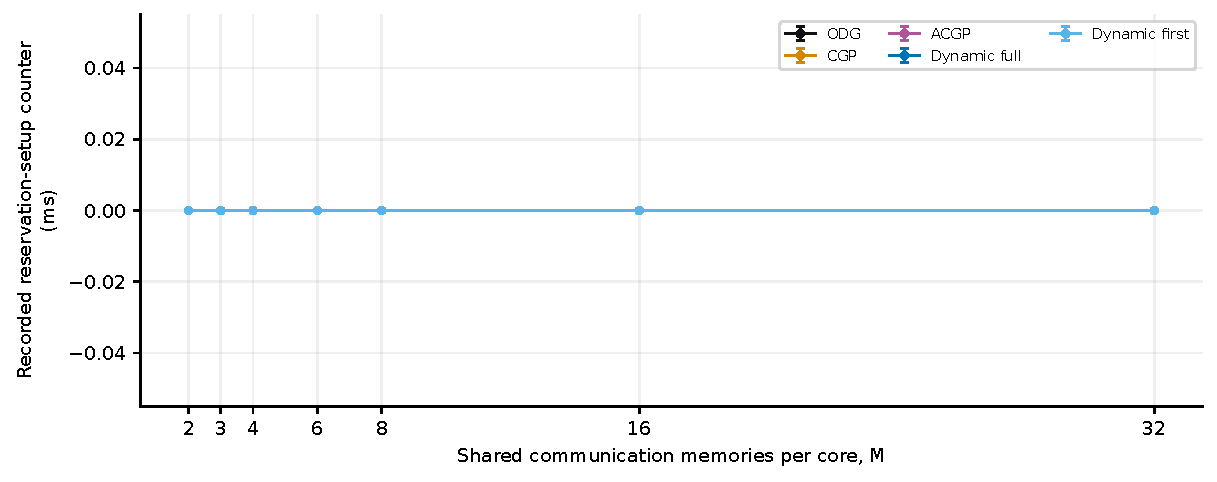
\includegraphics[width=.94\linewidth,height=.255\textheight,keepaspectratio]{figures/memory/mesh_yx_avg_reservation_setup_time_ms.pdf}\captionof{figure}{Run-level mean and sample SD. Shared trace aliases are counted once.}\end{center}
\begin{center}{\scriptsize\setlength{\tabcolsep}{3pt}
\begin{tabular}{lrrrrr}
\toprule
M & ODG & CGP & ACGP & Dynamic full & Dynamic first \\
\midrule
2 & $0.0000\pm0.0000$ & $0.0000\pm0.0000$ & $0.0000\pm0.0000$ & $0.0000\pm0.0000$ & $0.0000\pm0.0000$ \\
3 & $0.0000\pm0.0000$ & $0.0000\pm0.0000$ & $0.0000\pm0.0000$ & $0.0000\pm0.0000$ & $0.0000\pm0.0000$ \\
4 & $0.0000\pm0.0000$ & $0.0000\pm0.0000$ & $0.0000\pm0.0000$ & $0.0000\pm0.0000$ & $0.0000\pm0.0000$ \\
6 & $0.0000\pm0.0000$ & $0.0000\pm0.0000$ & $0.0000\pm0.0000$ & $0.0000\pm0.0000$ & $0.0000\pm0.0000$ \\
8 & $0.0000\pm0.0000$ & $0.0000\pm0.0000$ & $0.0000\pm0.0000$ & $0.0000\pm0.0000$ & $0.0000\pm0.0000$ \\
16 & $0.0000\pm0.0000$ & $0.0000\pm0.0000$ & $0.0000\pm0.0000$ & $0.0000\pm0.0000$ & $0.0000\pm0.0000$ \\
32 & $0.0000\pm0.0000$ & $0.0000\pm0.0000$ & $0.0000\pm0.0000$ & $0.0000\pm0.0000$ & $0.0000\pm0.0000$ \\
\bottomrule\end{tabular}}
\captionof{table}{Mean $\pm$ sample SD; n/a denotes a metric outside that policy's instrumentation.}
{\footnotesize\href{https://github.com/sanjeevkrishnaa/Compiler-Driven-ACE/blob/codex/ace-scheduler-correctness/docs/latex/qft96_final/data/memory_mesh_yx_avg_reservation_setup_time_ms.csv}{Exact CSV values and sample counts}}
\end{center}
\subsection*{Mean generation/service time}
\begin{center}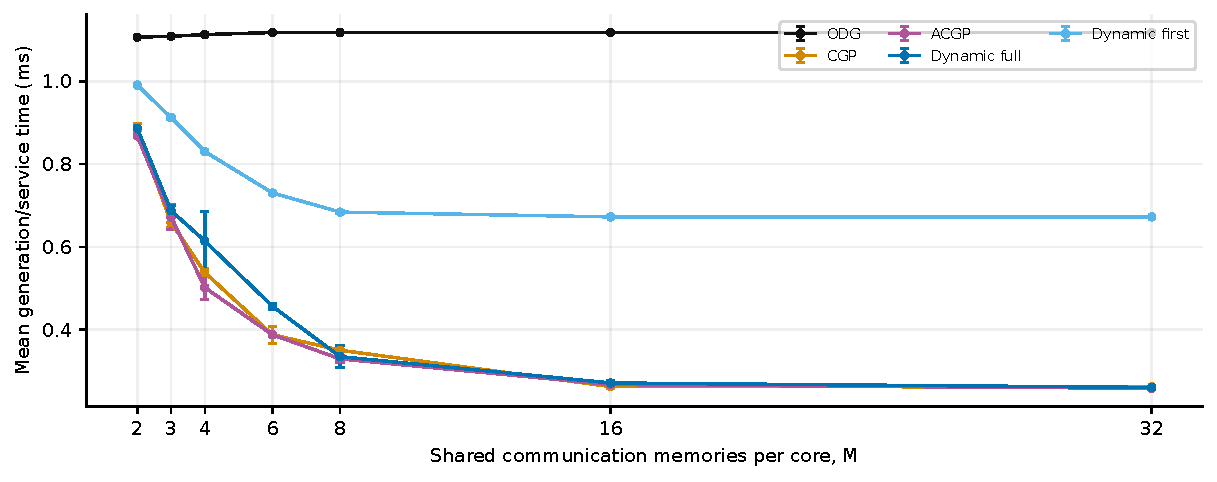
\includegraphics[width=.94\linewidth,height=.255\textheight,keepaspectratio]{figures/memory/mesh_yx_avg_entanglement_generation_time_ms.pdf}\captionof{figure}{Run-level mean and sample SD. Shared trace aliases are counted once.}\end{center}
\begin{center}{\scriptsize\setlength{\tabcolsep}{3pt}
\begin{tabular}{lrrrrr}
\toprule
M & ODG & CGP & ACGP & Dynamic full & Dynamic first \\
\midrule
2 & $1.106\pm0.000$ & $0.8831\pm0.0155$ & $0.8679\pm0.0006$ & $0.8866\pm0.0024$ & $0.9907\pm0.0007$ \\
3 & $1.109\pm0.000$ & $0.6591\pm0.0124$ & $0.6720\pm0.0296$ & $0.6876\pm0.0120$ & $0.9122\pm0.0037$ \\
4 & $1.113\pm0.002$ & $0.5381\pm0.0104$ & $0.5018\pm0.0279$ & $0.6142\pm0.0718$ & $0.8301\pm0.0028$ \\
6 & $1.118\pm0.000$ & $0.3878\pm0.0210$ & $0.3878\pm0.0002$ & $0.4565\pm0.0067$ & $0.7303\pm0.0022$ \\
8 & $1.118\pm0.000$ & $0.3505\pm0.0028$ & $0.3295\pm0.0074$ & $0.3349\pm0.0267$ & $0.6840\pm0.0037$ \\
16 & $1.118\pm0.000$ & $0.2627\pm0.0052$ & $0.2676\pm0.0012$ & $0.2715\pm0.0052$ & $0.6724\pm0.0011$ \\
32 & $1.118\pm0.000$ & $0.2620\pm0.0002$ & $0.2585\pm0.0008$ & $0.2606\pm0.0010$ & $0.6724\pm0.0011$ \\
\bottomrule\end{tabular}}
\captionof{table}{Mean $\pm$ sample SD; n/a denotes a metric outside that policy's instrumentation.}
{\footnotesize\href{https://github.com/sanjeevkrishnaa/Compiler-Driven-ACE/blob/codex/ace-scheduler-correctness/docs/latex/qft96_final/data/memory_mesh_yx_avg_entanglement_generation_time_ms.csv}{Exact CSV values and sample counts}}
\end{center}
\clearpage
\subsection*{Recorded retry-wait time}
\begin{center}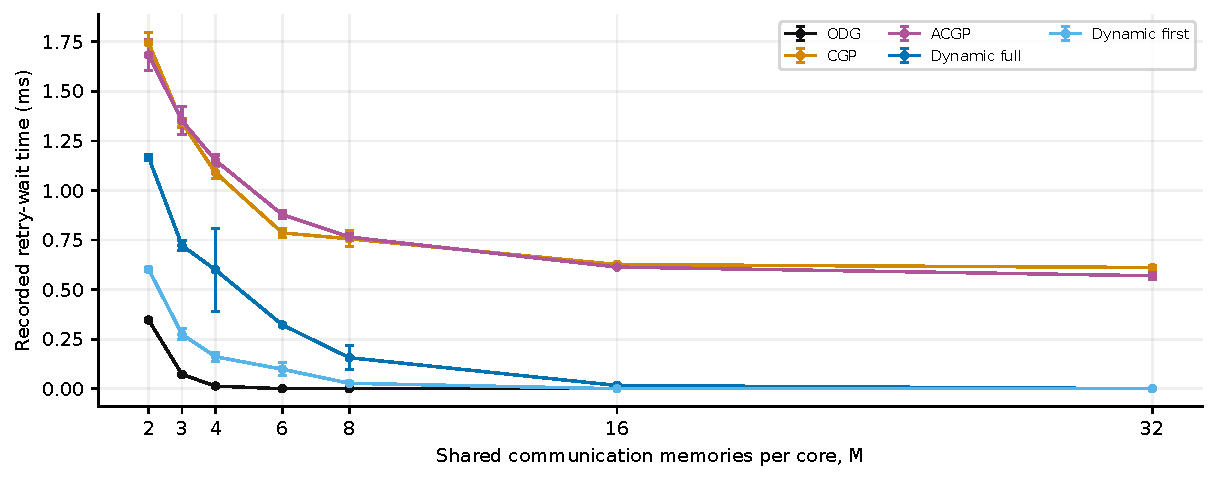
\includegraphics[width=.94\linewidth,height=.255\textheight,keepaspectratio]{figures/memory/mesh_yx_avg_retry_wait_time_ms.pdf}\captionof{figure}{Run-level mean and sample SD. Shared trace aliases are counted once.}\end{center}
\begin{center}{\scriptsize\setlength{\tabcolsep}{3pt}
\begin{tabular}{lrrrrr}
\toprule
M & ODG & CGP & ACGP & Dynamic full & Dynamic first \\
\midrule
2 & $0.3471\pm0.0048$ & $1.744\pm0.054$ & $1.683\pm0.077$ & $1.167\pm0.016$ & $0.6028\pm0.0088$ \\
3 & $0.0722\pm0.0055$ & $1.343\pm0.022$ & $1.352\pm0.069$ & $0.7225\pm0.0260$ & $0.2750\pm0.0290$ \\
4 & $0.0133\pm0.0009$ & $1.090\pm0.030$ & $1.152\pm0.027$ & $0.5996\pm0.2099$ & $0.1616\pm0.0227$ \\
6 & $0.0000\pm0.0000$ & $0.7861\pm0.0227$ & $0.8781\pm0.0188$ & $0.3220\pm0.0051$ & $0.0983\pm0.0326$ \\
8 & $0.0000\pm0.0000$ & $0.7562\pm0.0396$ & $0.7651\pm0.0183$ & $0.1567\pm0.0618$ & $0.0275\pm0.0080$ \\
16 & $0.0000\pm0.0000$ & $0.6264\pm0.0058$ & $0.6138\pm0.0041$ & $0.0165\pm0.0049$ & $0.0001\pm0.0001$ \\
32 & $0.0000\pm0.0000$ & $0.6115\pm0.0121$ & $0.5697\pm0.0179$ & $0.0001\pm0.0002$ & $0.0000\pm0.0000$ \\
\bottomrule\end{tabular}}
\captionof{table}{Mean $\pm$ sample SD; n/a denotes a metric outside that policy's instrumentation.}
{\footnotesize\href{https://github.com/sanjeevkrishnaa/Compiler-Driven-ACE/blob/codex/ace-scheduler-correctness/docs/latex/qft96_final/data/memory_mesh_yx_avg_retry_wait_time_ms.csv}{Exact CSV values and sample counts}}
\end{center}
\subsection*{Request retries}
\begin{center}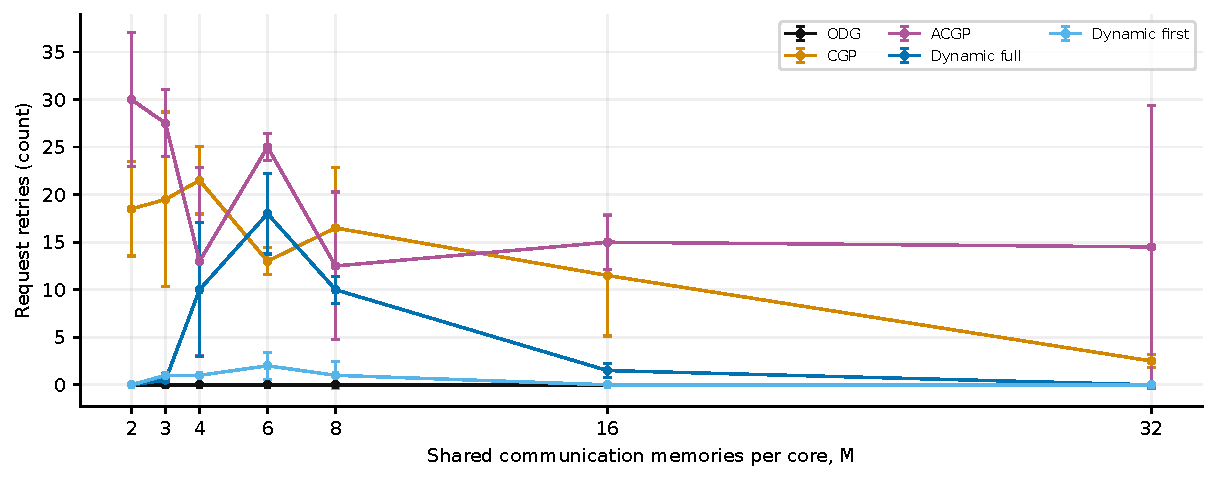
\includegraphics[width=.94\linewidth,height=.255\textheight,keepaspectratio]{figures/memory/mesh_yx_total_retries.pdf}\captionof{figure}{Run-level mean and sample SD. Shared trace aliases are counted once.}\end{center}
\begin{center}{\scriptsize\setlength{\tabcolsep}{3pt}
\begin{tabular}{lrrrrr}
\toprule
M & ODG & CGP & ACGP & Dynamic full & Dynamic first \\
\midrule
2 & $0.0000\pm0.0000$ & $18.500\pm4.950$ & $30.000\pm7.071$ & $0.0000\pm0.0000$ & $0.0000\pm0.0000$ \\
3 & $0.0000\pm0.0000$ & $19.500\pm9.192$ & $27.500\pm3.536$ & $0.5000\pm0.7071$ & $1.000\pm0.000$ \\
4 & $0.0000\pm0.0000$ & $21.500\pm3.536$ & $13.000\pm9.899$ & $10.000\pm7.071$ & $1.000\pm0.000$ \\
6 & $0.0000\pm0.0000$ & $13.000\pm1.414$ & $25.000\pm1.414$ & $18.000\pm4.243$ & $2.000\pm1.414$ \\
8 & $0.0000\pm0.0000$ & $16.500\pm6.364$ & $12.500\pm7.778$ & $10.000\pm1.414$ & $1.000\pm1.414$ \\
16 & $0.0000\pm0.0000$ & $11.500\pm6.364$ & $15.000\pm2.828$ & $1.500\pm0.707$ & $0.0000\pm0.0000$ \\
32 & $0.0000\pm0.0000$ & $2.500\pm0.707$ & $14.500\pm14.849$ & $0.0000\pm0.0000$ & $0.0000\pm0.0000$ \\
\bottomrule\end{tabular}}
\captionof{table}{Mean $\pm$ sample SD; n/a denotes a metric outside that policy's instrumentation.}
{\footnotesize\href{https://github.com/sanjeevkrishnaa/Compiler-Driven-ACE/blob/codex/ace-scheduler-correctness/docs/latex/qft96_final/data/memory_mesh_yx_total_retries.csv}{Exact CSV values and sample counts}}
\end{center}
\clearpage
\subsection*{Requests with retries}
\begin{center}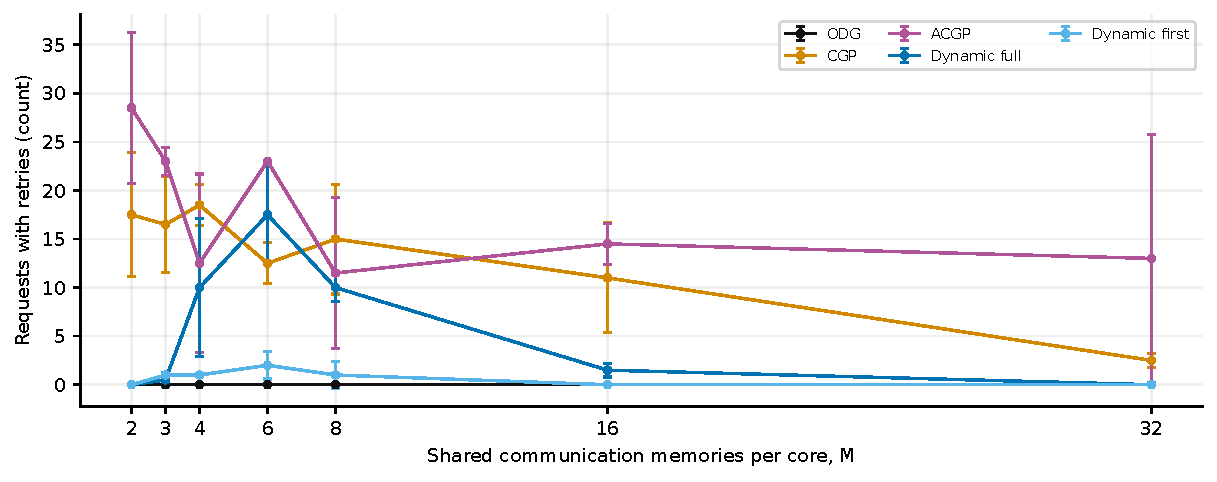
\includegraphics[width=.94\linewidth,height=.255\textheight,keepaspectratio]{figures/memory/mesh_yx_requests_with_retries.pdf}\captionof{figure}{Run-level mean and sample SD. Shared trace aliases are counted once.}\end{center}
\begin{center}{\scriptsize\setlength{\tabcolsep}{3pt}
\begin{tabular}{lrrrrr}
\toprule
M & ODG & CGP & ACGP & Dynamic full & Dynamic first \\
\midrule
2 & $0.0000\pm0.0000$ & $17.500\pm6.364$ & $28.500\pm7.778$ & $0.0000\pm0.0000$ & $0.0000\pm0.0000$ \\
3 & $0.0000\pm0.0000$ & $16.500\pm4.950$ & $23.000\pm1.414$ & $0.5000\pm0.7071$ & $1.000\pm0.000$ \\
4 & $0.0000\pm0.0000$ & $18.500\pm2.121$ & $12.500\pm9.192$ & $10.000\pm7.071$ & $1.000\pm0.000$ \\
6 & $0.0000\pm0.0000$ & $12.500\pm2.121$ & $23.000\pm0.000$ & $17.500\pm4.950$ & $2.000\pm1.414$ \\
8 & $0.0000\pm0.0000$ & $15.000\pm5.657$ & $11.500\pm7.778$ & $10.000\pm1.414$ & $1.000\pm1.414$ \\
16 & $0.0000\pm0.0000$ & $11.000\pm5.657$ & $14.500\pm2.121$ & $1.500\pm0.707$ & $0.0000\pm0.0000$ \\
32 & $0.0000\pm0.0000$ & $2.500\pm0.707$ & $13.000\pm12.728$ & $0.0000\pm0.0000$ & $0.0000\pm0.0000$ \\
\bottomrule\end{tabular}}
\captionof{table}{Mean $\pm$ sample SD; n/a denotes a metric outside that policy's instrumentation.}
{\footnotesize\href{https://github.com/sanjeevkrishnaa/Compiler-Driven-ACE/blob/codex/ace-scheduler-correctness/docs/latex/qft96_final/data/memory_mesh_yx_requests_with_retries.csv}{Exact CSV values and sample counts}}
\end{center}
\subsection*{Native-protocol generated-pair counter}
\begin{center}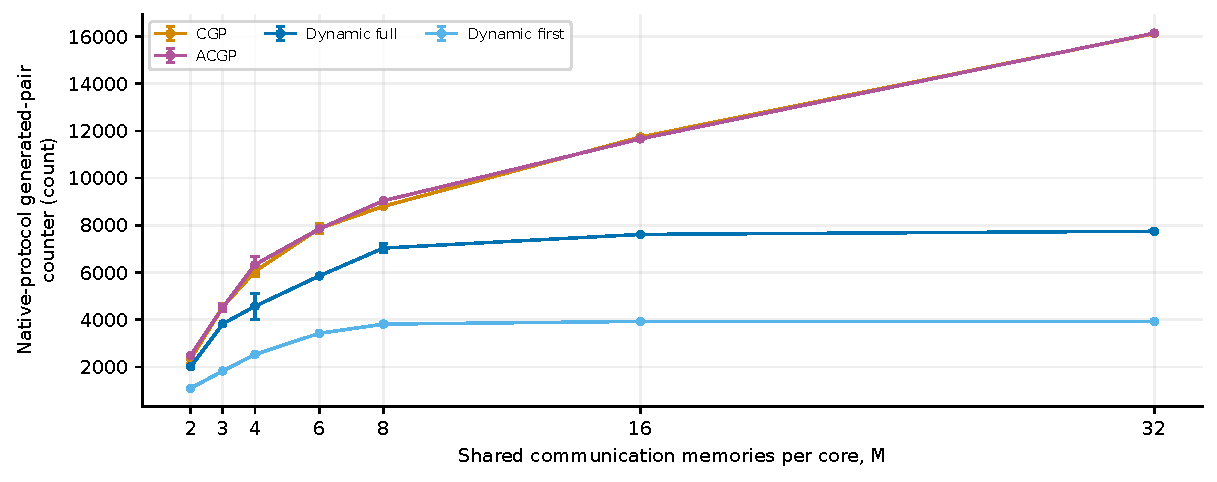
\includegraphics[width=.94\linewidth,height=.255\textheight,keepaspectratio]{figures/memory/mesh_yx_protocol_generated_pairs.pdf}\captionof{figure}{Run-level mean and sample SD. Shared trace aliases are counted once.}\end{center}
\begin{center}{\scriptsize\setlength{\tabcolsep}{3pt}
\begin{tabular}{lrrrrr}
\toprule
M & ODG & CGP & ACGP & Dynamic full & Dynamic first \\
\midrule
2 & n/a & $2337.00\pm173.95$ & $2485.00\pm38.18$ & $2010.00\pm48.08$ & $1099.00\pm21.21$ \\
3 & n/a & $4547.00\pm120.21$ & $4517.00\pm185.26$ & $3828.00\pm14.14$ & $1831.00\pm9.90$ \\
4 & n/a & $6046.00\pm197.99$ & $6333.00\pm357.80$ & $4570.00\pm560.03$ & $2534.00\pm5.66$ \\
6 & n/a & $7864.00\pm214.96$ & $7850.00\pm5.66$ & $5855.00\pm32.53$ & $3426.00\pm28.28$ \\
8 & n/a & $8806.00\pm31.11$ & $9042.00\pm70.71$ & $7037.00\pm199.40$ & $3816.00\pm73.54$ \\
16 & n/a & $11741.00\pm55.15$ & $11663.00\pm1.41$ & $7616.00\pm33.94$ & $3930.00\pm0.00$ \\
32 & n/a & $16125.00\pm52.33$ & $16142.00\pm25.46$ & $7752.00\pm0.00$ & $3930.00\pm0.00$ \\
\bottomrule\end{tabular}}
\captionof{table}{Mean $\pm$ sample SD; n/a denotes a metric outside that policy's instrumentation.}
{\footnotesize\href{https://github.com/sanjeevkrishnaa/Compiler-Driven-ACE/blob/codex/ace-scheduler-correctness/docs/latex/qft96_final/data/memory_mesh_yx_protocol_generated_pairs.csv}{Exact CSV values and sample counts}}
\end{center}
\clearpage
\subsection*{Native-protocol used-pair counter}
\begin{center}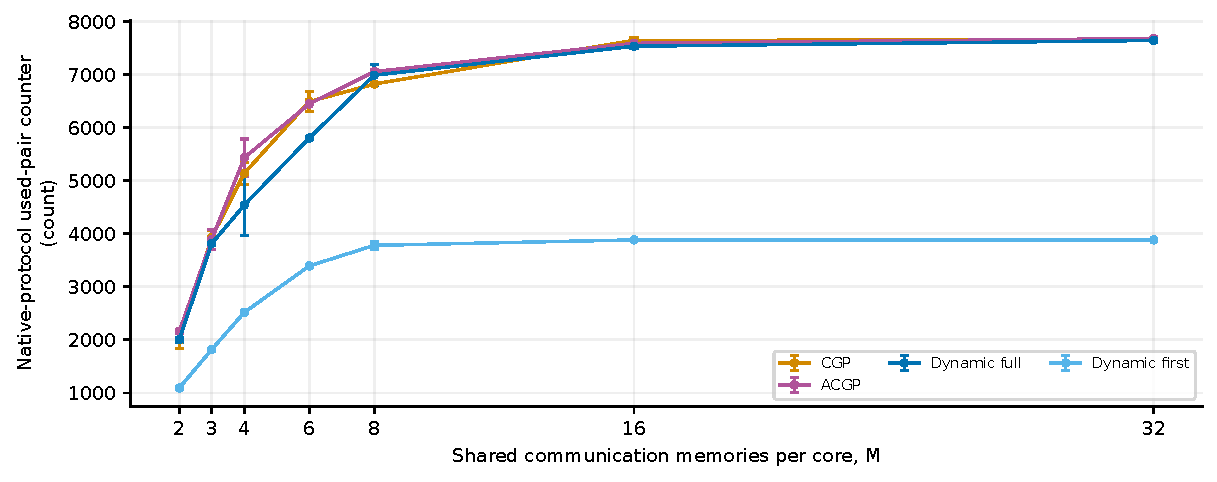
\includegraphics[width=.94\linewidth,height=.255\textheight,keepaspectratio]{figures/memory/mesh_yx_protocol_used_pairs.pdf}\captionof{figure}{Run-level mean and sample SD. Shared trace aliases are counted once.}\end{center}
\begin{center}{\scriptsize\setlength{\tabcolsep}{3pt}
\begin{tabular}{lrrrrr}
\toprule
M & ODG & CGP & ACGP & Dynamic full & Dynamic first \\
\midrule
2 & n/a & $1998.00\pm169.71$ & $2159.00\pm38.18$ & $2004.00\pm48.08$ & $1092.00\pm19.80$ \\
3 & n/a & $3930.00\pm132.94$ & $3895.00\pm185.26$ & $3816.00\pm11.31$ & $1819.00\pm9.90$ \\
4 & n/a & $5140.00\pm206.48$ & $5435.00\pm352.14$ & $4540.00\pm568.51$ & $2516.00\pm5.66$ \\
6 & n/a & $6492.00\pm192.33$ & $6448.00\pm14.14$ & $5805.00\pm32.53$ & $3393.00\pm32.53$ \\
8 & n/a & $6823.00\pm9.90$ & $7057.00\pm38.18$ & $6990.00\pm197.99$ & $3781.00\pm80.61$ \\
16 & n/a & $7648.00\pm48.08$ & $7591.00\pm7.07$ & $7536.00\pm33.94$ & $3884.00\pm8.49$ \\
32 & n/a & $7651.00\pm12.73$ & $7681.00\pm12.73$ & $7645.00\pm9.90$ & $3884.00\pm8.49$ \\
\bottomrule\end{tabular}}
\captionof{table}{Mean $\pm$ sample SD; n/a denotes a metric outside that policy's instrumentation.}
{\footnotesize\href{https://github.com/sanjeevkrishnaa/Compiler-Driven-ACE/blob/codex/ace-scheduler-correctness/docs/latex/qft96_final/data/memory_mesh_yx_protocol_used_pairs.csv}{Exact CSV values and sample counts}}
\end{center}
\subsection*{Native-protocol unused-pair counter}
\begin{center}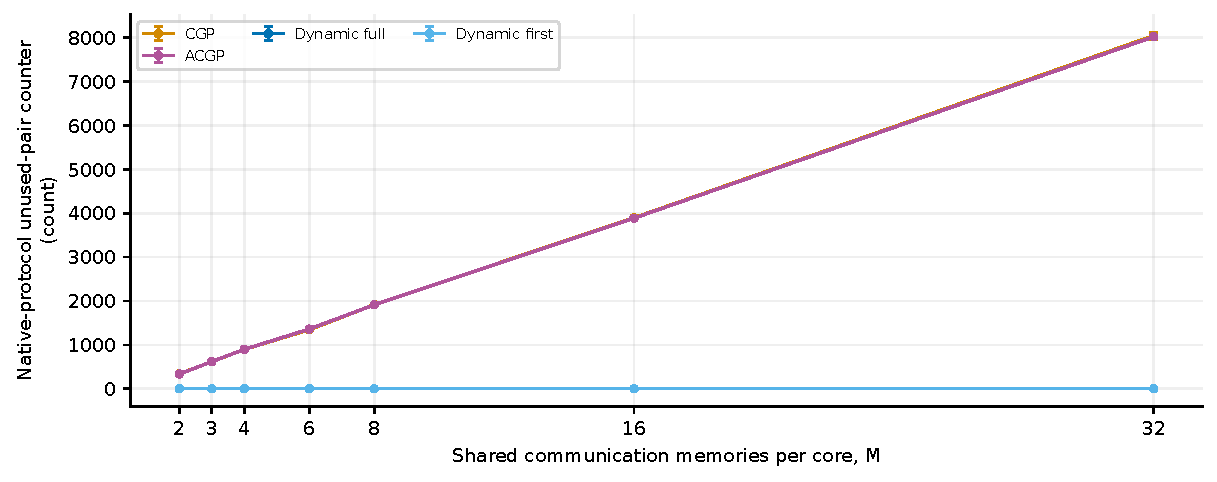
\includegraphics[width=.94\linewidth,height=.255\textheight,keepaspectratio]{figures/memory/mesh_yx_protocol_unused_pairs.pdf}\captionof{figure}{Run-level mean and sample SD. Shared trace aliases are counted once.}\end{center}
\begin{center}{\scriptsize\setlength{\tabcolsep}{3pt}
\begin{tabular}{lrrrrr}
\toprule
M & ODG & CGP & ACGP & Dynamic full & Dynamic first \\
\midrule
2 & n/a & $340.00\pm2.83$ & $335.00\pm1.41$ & $0.0000\pm0.0000$ & $0.0000\pm0.0000$ \\
3 & n/a & $617.00\pm7.07$ & $618.00\pm8.49$ & $0.0000\pm0.0000$ & $0.0000\pm0.0000$ \\
4 & n/a & $898.00\pm8.49$ & $897.00\pm1.41$ & $0.0000\pm0.0000$ & $0.0000\pm0.0000$ \\
6 & n/a & $1344.00\pm19.80$ & $1360.00\pm8.49$ & $0.0000\pm0.0000$ & $0.0000\pm0.0000$ \\
8 & n/a & $1916.00\pm5.66$ & $1914.00\pm19.80$ & $0.0000\pm0.0000$ & $0.0000\pm0.0000$ \\
16 & n/a & $3896.00\pm0.00$ & $3888.00\pm8.49$ & $0.0000\pm0.0000$ & $0.0000\pm0.0000$ \\
32 & n/a & $8048.00\pm76.37$ & $8025.00\pm46.67$ & $0.0000\pm0.0000$ & $0.0000\pm0.0000$ \\
\bottomrule\end{tabular}}
\captionof{table}{Mean $\pm$ sample SD; n/a denotes a metric outside that policy's instrumentation.}
{\footnotesize\href{https://github.com/sanjeevkrishnaa/Compiler-Driven-ACE/blob/codex/ace-scheduler-correctness/docs/latex/qft96_final/data/memory_mesh_yx_protocol_unused_pairs.csv}{Exact CSV values and sample counts}}
\end{center}
\clearpage
\subsection*{Scheduled compiler preparations}
\begin{center}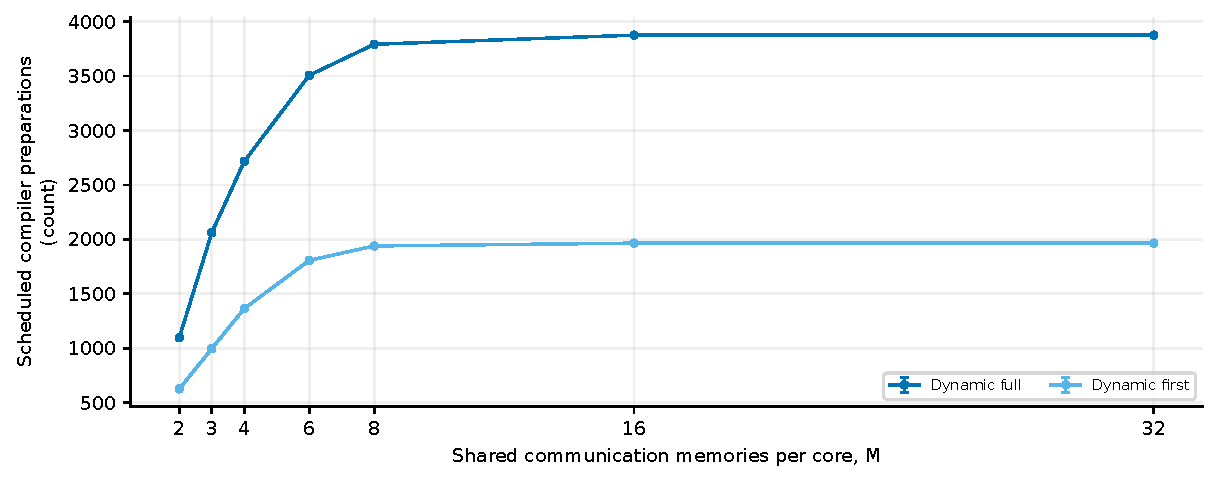
\includegraphics[width=.94\linewidth,height=.255\textheight,keepaspectratio]{figures/memory/mesh_yx_scheduled_preparations.pdf}\captionof{figure}{Run-level mean and sample SD. Shared trace aliases are counted once.}\end{center}
\begin{center}{\scriptsize\setlength{\tabcolsep}{3pt}
\begin{tabular}{lrrrrr}
\toprule
M & ODG & CGP & ACGP & Dynamic full & Dynamic first \\
\midrule
2 & n/a & n/a & n/a & $1097.00\pm0.00$ & $626.00\pm0.00$ \\
3 & n/a & n/a & n/a & $2062.00\pm0.00$ & $996.00\pm0.00$ \\
4 & n/a & n/a & n/a & $2716.00\pm0.00$ & $1364.00\pm0.00$ \\
6 & n/a & n/a & n/a & $3507.00\pm0.00$ & $1807.00\pm0.00$ \\
8 & n/a & n/a & n/a & $3792.00\pm0.00$ & $1939.00\pm0.00$ \\
16 & n/a & n/a & n/a & $3876.00\pm0.00$ & $1965.00\pm0.00$ \\
32 & n/a & n/a & n/a & $3876.00\pm0.00$ & $1965.00\pm0.00$ \\
\bottomrule\end{tabular}}
\captionof{table}{Mean $\pm$ sample SD; n/a denotes a metric outside that policy's instrumentation.}
{\footnotesize\href{https://github.com/sanjeevkrishnaa/Compiler-Driven-ACE/blob/codex/ace-scheduler-correctness/docs/latex/qft96_final/data/memory_mesh_yx_scheduled_preparations.csv}{Exact CSV values and sample counts}}
\end{center}
\subsection*{Planner-blocked preparations}
\begin{center}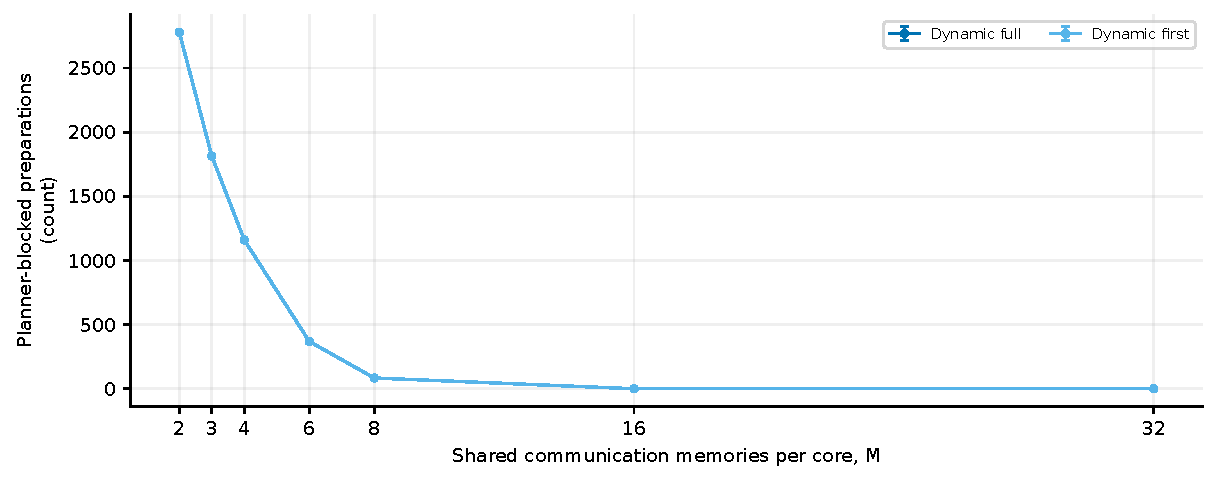
\includegraphics[width=.94\linewidth,height=.255\textheight,keepaspectratio]{figures/memory/mesh_yx_planner_blocked_preparations.pdf}\captionof{figure}{Run-level mean and sample SD. Shared trace aliases are counted once.}\end{center}
\begin{center}{\scriptsize\setlength{\tabcolsep}{3pt}
\begin{tabular}{lrrrrr}
\toprule
M & ODG & CGP & ACGP & Dynamic full & Dynamic first \\
\midrule
2 & n/a & n/a & n/a & $2779.00\pm0.00$ & $2779.00\pm0.00$ \\
3 & n/a & n/a & n/a & $1814.00\pm0.00$ & $1814.00\pm0.00$ \\
4 & n/a & n/a & n/a & $1160.00\pm0.00$ & $1160.00\pm0.00$ \\
6 & n/a & n/a & n/a & $369.00\pm0.00$ & $369.00\pm0.00$ \\
8 & n/a & n/a & n/a & $84.000\pm0.000$ & $84.000\pm0.000$ \\
16 & n/a & n/a & n/a & $0.0000\pm0.0000$ & $0.0000\pm0.0000$ \\
32 & n/a & n/a & n/a & $0.0000\pm0.0000$ & $0.0000\pm0.0000$ \\
\bottomrule\end{tabular}}
\captionof{table}{Mean $\pm$ sample SD; n/a denotes a metric outside that policy's instrumentation.}
{\footnotesize\href{https://github.com/sanjeevkrishnaa/Compiler-Driven-ACE/blob/codex/ace-scheduler-correctness/docs/latex/qft96_final/data/memory_mesh_yx_planner_blocked_preparations.csv}{Exact CSV values and sample counts}}
\end{center}
\clearpage
\subsection*{Planner peak compiler memory}
\begin{center}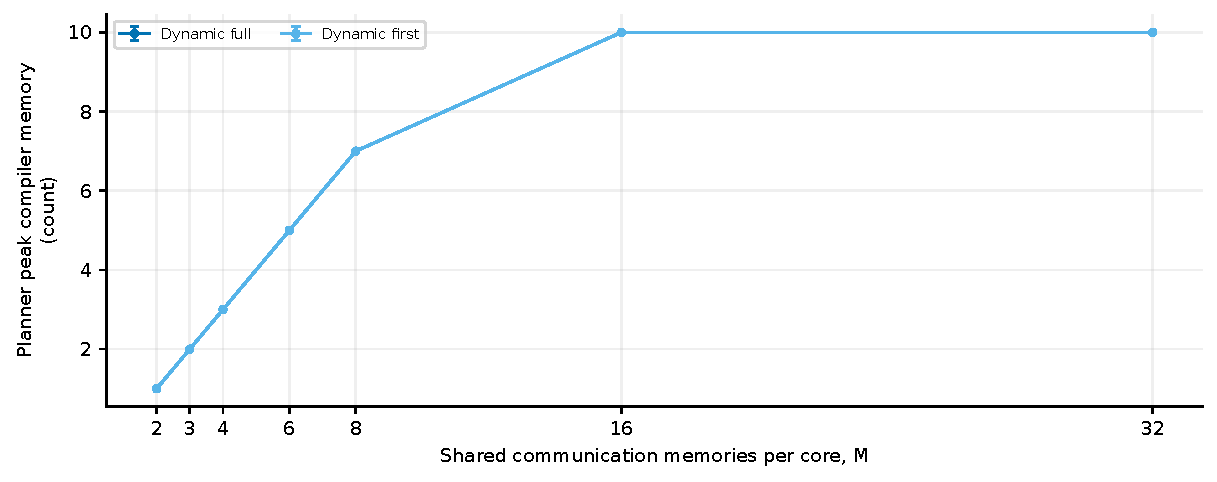
\includegraphics[width=.94\linewidth,height=.255\textheight,keepaspectratio]{figures/memory/mesh_yx_planner_peak_compiler_memory_per_core.pdf}\captionof{figure}{Run-level mean and sample SD. Shared trace aliases are counted once.}\end{center}
\begin{center}{\scriptsize\setlength{\tabcolsep}{3pt}
\begin{tabular}{lrrrrr}
\toprule
M & ODG & CGP & ACGP & Dynamic full & Dynamic first \\
\midrule
2 & n/a & n/a & n/a & $1.000\pm0.000$ & $1.000\pm0.000$ \\
3 & n/a & n/a & n/a & $2.000\pm0.000$ & $2.000\pm0.000$ \\
4 & n/a & n/a & n/a & $3.000\pm0.000$ & $3.000\pm0.000$ \\
6 & n/a & n/a & n/a & $5.000\pm0.000$ & $5.000\pm0.000$ \\
8 & n/a & n/a & n/a & $7.000\pm0.000$ & $7.000\pm0.000$ \\
16 & n/a & n/a & n/a & $10.000\pm0.000$ & $10.000\pm0.000$ \\
32 & n/a & n/a & n/a & $10.000\pm0.000$ & $10.000\pm0.000$ \\
\bottomrule\end{tabular}}
\captionof{table}{Mean $\pm$ sample SD; n/a denotes a metric outside that policy's instrumentation.}
{\footnotesize\href{https://github.com/sanjeevkrishnaa/Compiler-Driven-ACE/blob/codex/ace-scheduler-correctness/docs/latex/qft96_final/data/memory_mesh_yx_planner_peak_compiler_memory_per_core.csv}{Exact CSV values and sample counts}}
\end{center}
\subsection*{Compiler preparation admission attempts}
\begin{center}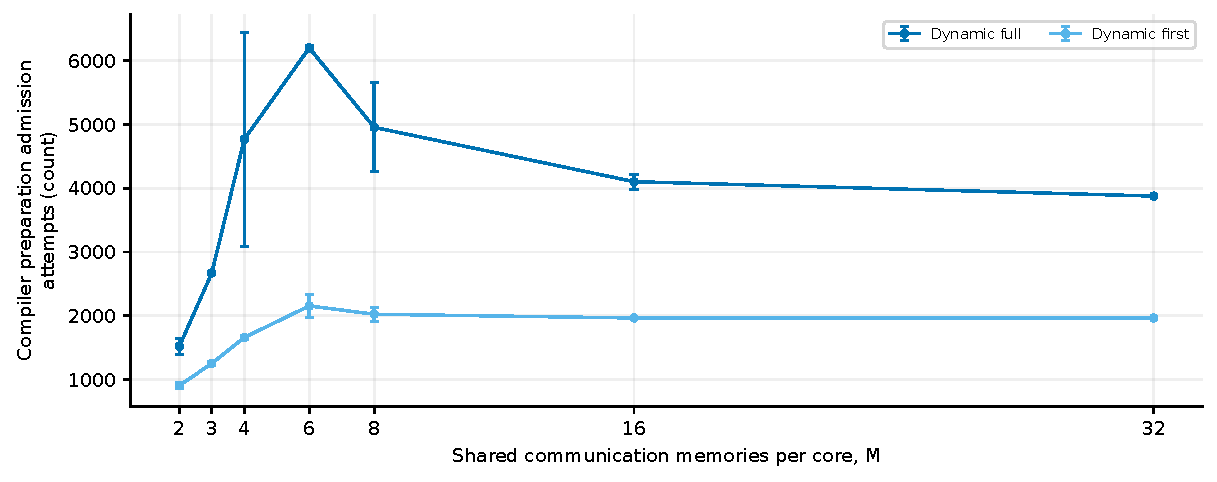
\includegraphics[width=.94\linewidth,height=.255\textheight,keepaspectratio]{figures/memory/mesh_yx_runtime_admission_attempts.pdf}\captionof{figure}{Run-level mean and sample SD. Shared trace aliases are counted once.}\end{center}
\begin{center}{\scriptsize\setlength{\tabcolsep}{3pt}
\begin{tabular}{lrrrrr}
\toprule
M & ODG & CGP & ACGP & Dynamic full & Dynamic first \\
\midrule
2 & n/a & n/a & n/a & $1519.50\pm125.16$ & $907.50\pm51.62$ \\
3 & n/a & n/a & n/a & $2670.50\pm26.16$ & $1251.50\pm34.65$ \\
4 & n/a & n/a & n/a & $4766.50\pm1676.55$ & $1659.50\pm27.58$ \\
6 & n/a & n/a & n/a & $6198.50\pm40.31$ & $2154.00\pm185.26$ \\
8 & n/a & n/a & n/a & $4953.50\pm697.91$ & $2024.00\pm111.72$ \\
16 & n/a & n/a & n/a & $4102.00\pm118.79$ & $1965.00\pm0.00$ \\
32 & n/a & n/a & n/a & $3876.00\pm0.00$ & $1965.00\pm0.00$ \\
\bottomrule\end{tabular}}
\captionof{table}{Mean $\pm$ sample SD; n/a denotes a metric outside that policy's instrumentation.}
{\footnotesize\href{https://github.com/sanjeevkrishnaa/Compiler-Driven-ACE/blob/codex/ace-scheduler-correctness/docs/latex/qft96_final/data/memory_mesh_yx_runtime_admission_attempts.csv}{Exact CSV values and sample counts}}
\end{center}
\clearpage
\subsection*{Launched compiler preparations}
\begin{center}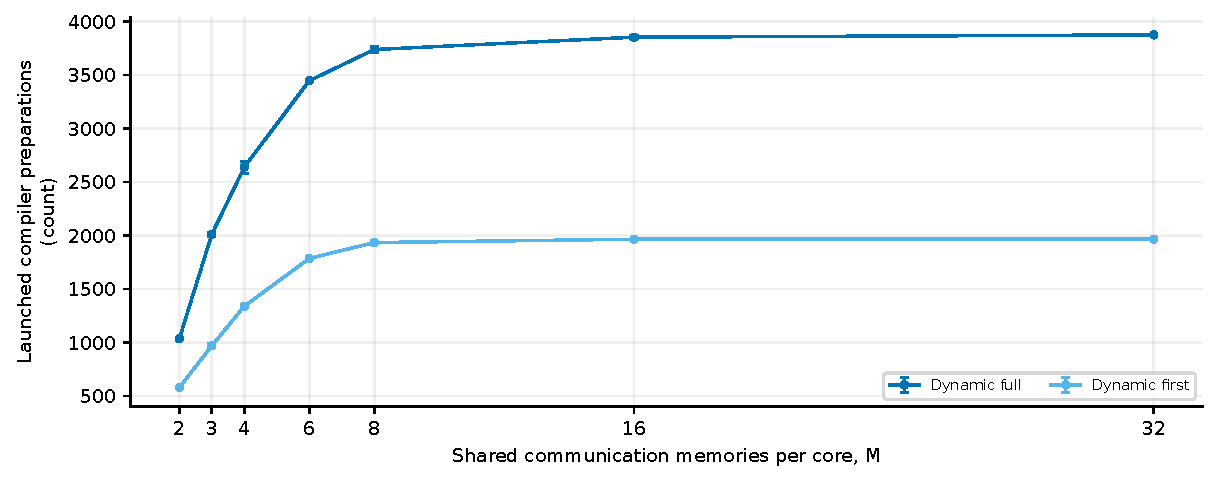
\includegraphics[width=.94\linewidth,height=.255\textheight,keepaspectratio]{figures/memory/mesh_yx_runtime_launched_preparations.pdf}\captionof{figure}{Run-level mean and sample SD. Shared trace aliases are counted once.}\end{center}
\begin{center}{\scriptsize\setlength{\tabcolsep}{3pt}
\begin{tabular}{lrrrrr}
\toprule
M & ODG & CGP & ACGP & Dynamic full & Dynamic first \\
\midrule
2 & n/a & n/a & n/a & $1035.00\pm2.83$ & $578.00\pm12.73$ \\
3 & n/a & n/a & n/a & $2010.50\pm19.09$ & $968.00\pm16.97$ \\
4 & n/a & n/a & n/a & $2639.00\pm55.15$ & $1338.00\pm7.07$ \\
6 & n/a & n/a & n/a & $3447.00\pm1.41$ & $1785.00\pm9.90$ \\
8 & n/a & n/a & n/a & $3739.00\pm24.04$ & $1933.50\pm6.36$ \\
16 & n/a & n/a & n/a & $3854.50\pm16.26$ & $1965.00\pm0.00$ \\
32 & n/a & n/a & n/a & $3876.00\pm0.00$ & $1965.00\pm0.00$ \\
\bottomrule\end{tabular}}
\captionof{table}{Mean $\pm$ sample SD; n/a denotes a metric outside that policy's instrumentation.}
{\footnotesize\href{https://github.com/sanjeevkrishnaa/Compiler-Driven-ACE/blob/codex/ace-scheduler-correctness/docs/latex/qft96_final/data/memory_mesh_yx_runtime_launched_preparations.csv}{Exact CSV values and sample counts}}
\end{center}
\subsection*{Accepted compiler preparations}
\begin{center}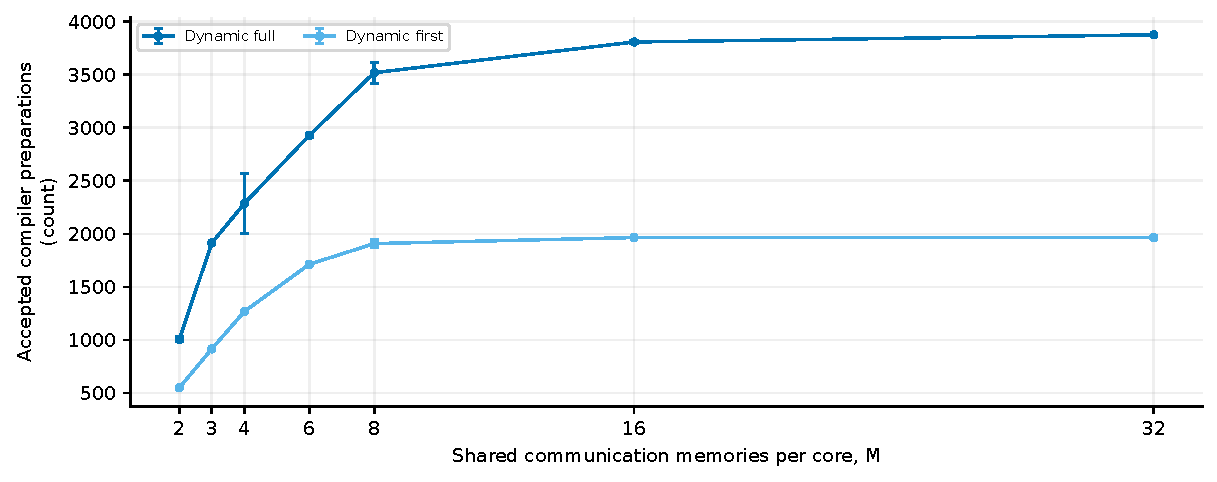
\includegraphics[width=.94\linewidth,height=.255\textheight,keepaspectratio]{figures/memory/mesh_yx_runtime_accepted_preparations.pdf}\captionof{figure}{Run-level mean and sample SD. Shared trace aliases are counted once.}\end{center}
\begin{center}{\scriptsize\setlength{\tabcolsep}{3pt}
\begin{tabular}{lrrrrr}
\toprule
M & ODG & CGP & ACGP & Dynamic full & Dynamic first \\
\midrule
2 & n/a & n/a & n/a & $1005.00\pm24.04$ & $549.50\pm10.61$ \\
3 & n/a & n/a & n/a & $1914.00\pm7.07$ & $915.50\pm4.95$ \\
4 & n/a & n/a & n/a & $2285.00\pm280.01$ & $1267.00\pm2.83$ \\
6 & n/a & n/a & n/a & $2927.50\pm16.26$ & $1713.00\pm14.14$ \\
8 & n/a & n/a & n/a & $3518.50\pm99.70$ & $1908.00\pm36.77$ \\
16 & n/a & n/a & n/a & $3808.00\pm16.97$ & $1965.00\pm0.00$ \\
32 & n/a & n/a & n/a & $3876.00\pm0.00$ & $1965.00\pm0.00$ \\
\bottomrule\end{tabular}}
\captionof{table}{Mean $\pm$ sample SD; n/a denotes a metric outside that policy's instrumentation.}
{\footnotesize\href{https://github.com/sanjeevkrishnaa/Compiler-Driven-ACE/blob/codex/ace-scheduler-correctness/docs/latex/qft96_final/data/memory_mesh_yx_runtime_accepted_preparations.csv}{Exact CSV values and sample counts}}
\end{center}
\clearpage
\subsection*{Rejected compiler preparations}
\begin{center}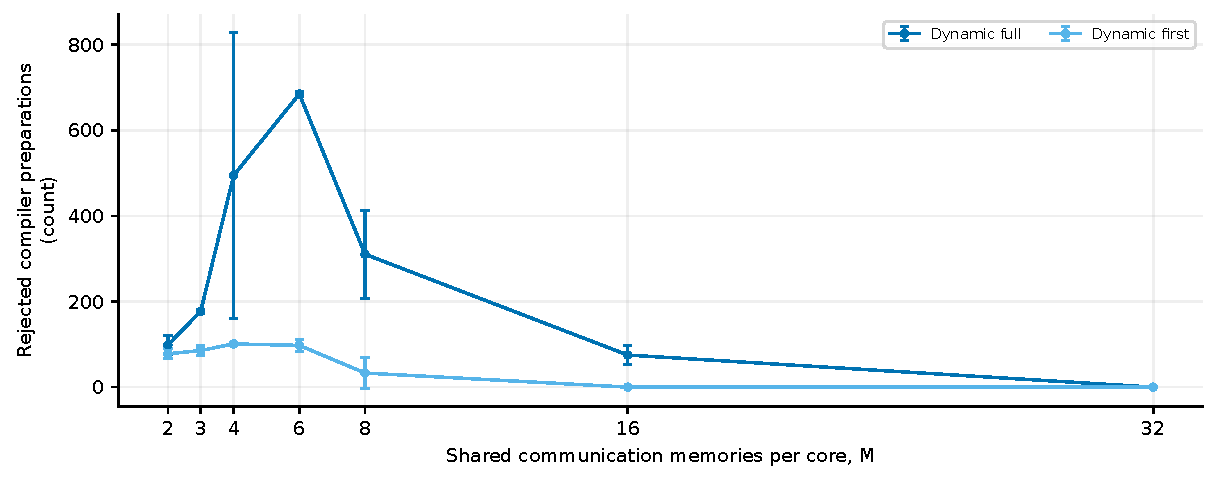
\includegraphics[width=.94\linewidth,height=.255\textheight,keepaspectratio]{figures/memory/mesh_yx_runtime_rejected_preparations.pdf}\captionof{figure}{Run-level mean and sample SD. Shared trace aliases are counted once.}\end{center}
\begin{center}{\scriptsize\setlength{\tabcolsep}{3pt}
\begin{tabular}{lrrrrr}
\toprule
M & ODG & CGP & ACGP & Dynamic full & Dynamic first \\
\midrule
2 & n/a & n/a & n/a & $98.500\pm21.920$ & $78.000\pm11.314$ \\
3 & n/a & n/a & n/a & $177.50\pm4.95$ & $85.500\pm10.607$ \\
4 & n/a & n/a & n/a & $494.50\pm334.46$ & $101.00\pm4.24$ \\
6 & n/a & n/a & n/a & $685.00\pm5.66$ & $97.500\pm14.849$ \\
8 & n/a & n/a & n/a & $310.50\pm102.53$ & $33.000\pm36.770$ \\
16 & n/a & n/a & n/a & $75.000\pm22.627$ & $0.0000\pm0.0000$ \\
32 & n/a & n/a & n/a & $0.0000\pm0.0000$ & $0.0000\pm0.0000$ \\
\bottomrule\end{tabular}}
\captionof{table}{Mean $\pm$ sample SD; n/a denotes a metric outside that policy's instrumentation.}
{\footnotesize\href{https://github.com/sanjeevkrishnaa/Compiler-Driven-ACE/blob/codex/ace-scheduler-correctness/docs/latex/qft96_final/data/memory_mesh_yx_runtime_rejected_preparations.csv}{Exact CSV values and sample counts}}
\end{center}
\subsection*{Compiler-ready request count}
\begin{center}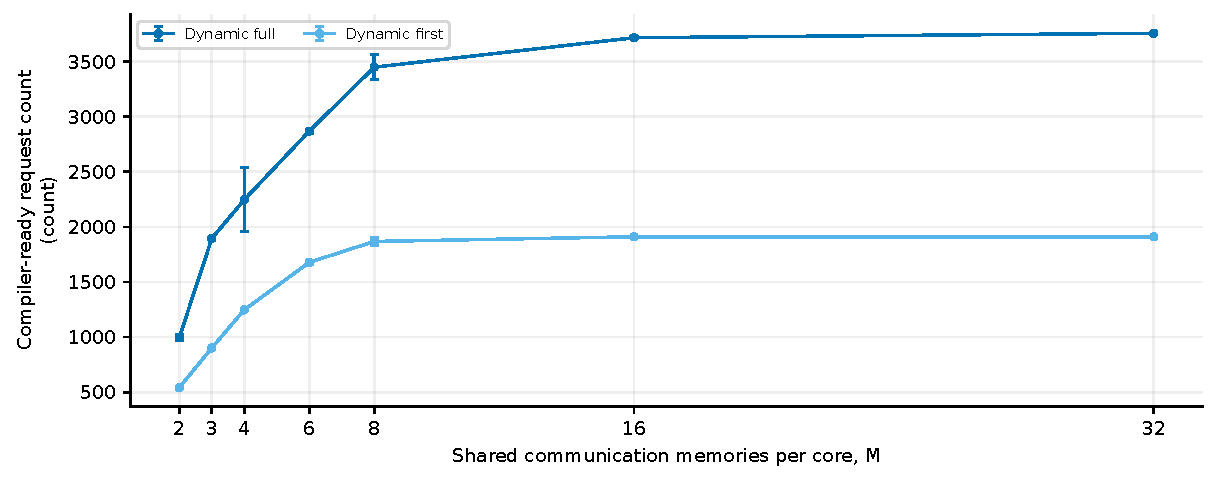
\includegraphics[width=.94\linewidth,height=.255\textheight,keepaspectratio]{figures/memory/mesh_yx_pregenerated_hits.pdf}\captionof{figure}{Run-level mean and sample SD. Shared trace aliases are counted once.}\end{center}
\begin{center}{\scriptsize\setlength{\tabcolsep}{3pt}
\begin{tabular}{lrrrrr}
\toprule
M & ODG & CGP & ACGP & Dynamic full & Dynamic first \\
\midrule
2 & n/a & n/a & n/a & $996.50\pm23.33$ & $542.00\pm9.90$ \\
3 & n/a & n/a & n/a & $1895.00\pm1.41$ & $902.50\pm2.12$ \\
4 & n/a & n/a & n/a & $2246.00\pm291.33$ & $1247.50\pm7.78$ \\
6 & n/a & n/a & n/a & $2867.00\pm16.97$ & $1678.00\pm16.97$ \\
8 & n/a & n/a & n/a & $3447.50\pm112.43$ & $1867.50\pm37.48$ \\
16 & n/a & n/a & n/a & $3714.50\pm10.61$ & $1910.00\pm4.24$ \\
32 & n/a & n/a & n/a & $3755.00\pm8.49$ & $1910.00\pm4.24$ \\
\bottomrule\end{tabular}}
\captionof{table}{Mean $\pm$ sample SD; n/a denotes a metric outside that policy's instrumentation.}
{\footnotesize\href{https://github.com/sanjeevkrishnaa/Compiler-Driven-ACE/blob/codex/ace-scheduler-correctness/docs/latex/qft96_final/data/memory_mesh_yx_pregenerated_hits.csv}{Exact CSV values and sample counts}}
\end{center}
\clearpage
\subsection*{Intended compiler-hit count}
\begin{center}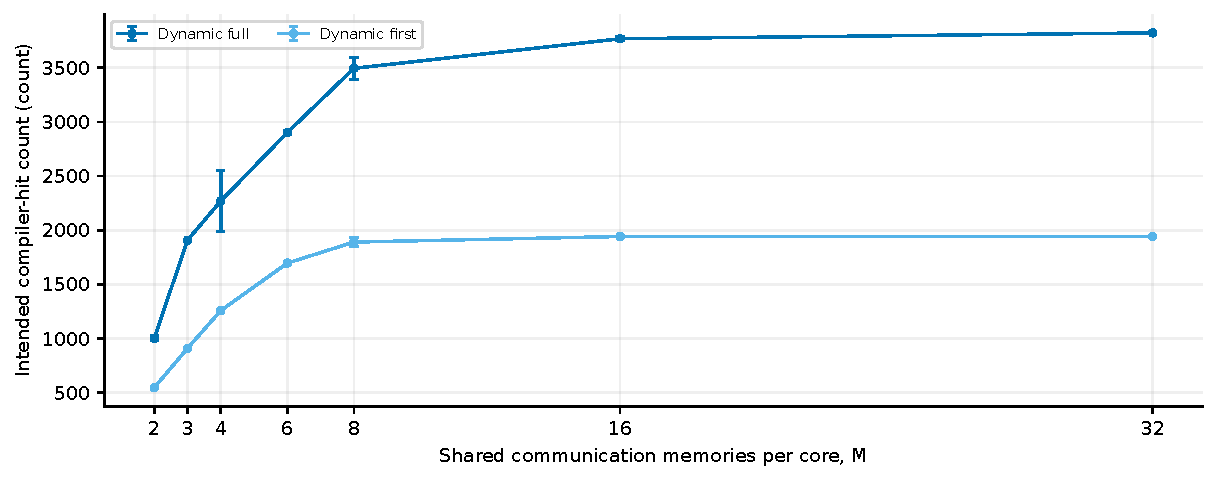
\includegraphics[width=.94\linewidth,height=.255\textheight,keepaspectratio]{figures/memory/mesh_yx_intended_request_hits.pdf}\captionof{figure}{Run-level mean and sample SD. Shared trace aliases are counted once.}\end{center}
\begin{center}{\scriptsize\setlength{\tabcolsep}{3pt}
\begin{tabular}{lrrrrr}
\toprule
M & ODG & CGP & ACGP & Dynamic full & Dynamic first \\
\midrule
2 & n/a & n/a & n/a & $1002.00\pm24.04$ & $546.00\pm9.90$ \\
3 & n/a & n/a & n/a & $1908.00\pm5.66$ & $909.50\pm4.95$ \\
4 & n/a & n/a & n/a & $2270.00\pm284.26$ & $1258.00\pm2.83$ \\
6 & n/a & n/a & n/a & $2902.50\pm16.26$ & $1696.50\pm16.26$ \\
8 & n/a & n/a & n/a & $3495.00\pm98.99$ & $1890.50\pm40.31$ \\
16 & n/a & n/a & n/a & $3768.00\pm16.97$ & $1942.00\pm4.24$ \\
32 & n/a & n/a & n/a & $3822.50\pm4.95$ & $1942.00\pm4.24$ \\
\bottomrule\end{tabular}}
\captionof{table}{Mean $\pm$ sample SD; n/a denotes a metric outside that policy's instrumentation.}
{\footnotesize\href{https://github.com/sanjeevkrishnaa/Compiler-Driven-ACE/blob/codex/ace-scheduler-correctness/docs/latex/qft96_final/data/memory_mesh_yx_intended_request_hits.csv}{Exact CSV values and sample counts}}
\end{center}
\subsection*{Compiler-not-ready request count}
\begin{center}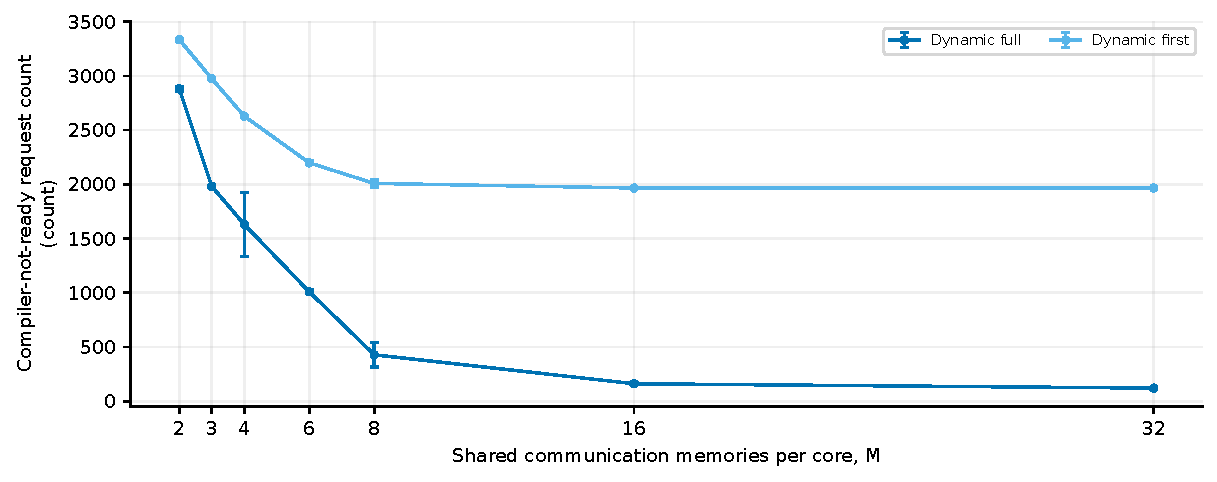
\includegraphics[width=.94\linewidth,height=.255\textheight,keepaspectratio]{figures/memory/mesh_yx_compiler_not_ready_requests.pdf}\captionof{figure}{Run-level mean and sample SD. Shared trace aliases are counted once.}\end{center}
\begin{center}{\scriptsize\setlength{\tabcolsep}{3pt}
\begin{tabular}{lrrrrr}
\toprule
M & ODG & CGP & ACGP & Dynamic full & Dynamic first \\
\midrule
2 & n/a & n/a & n/a & $2879.50\pm23.33$ & $3334.00\pm9.90$ \\
3 & n/a & n/a & n/a & $1981.00\pm1.41$ & $2973.50\pm2.12$ \\
4 & n/a & n/a & n/a & $1630.00\pm291.33$ & $2628.50\pm7.78$ \\
6 & n/a & n/a & n/a & $1009.00\pm16.97$ & $2198.00\pm16.97$ \\
8 & n/a & n/a & n/a & $428.50\pm112.43$ & $2008.50\pm37.48$ \\
16 & n/a & n/a & n/a & $161.50\pm10.61$ & $1966.00\pm4.24$ \\
32 & n/a & n/a & n/a & $121.00\pm8.49$ & $1966.00\pm4.24$ \\
\bottomrule\end{tabular}}
\captionof{table}{Mean $\pm$ sample SD; n/a denotes a metric outside that policy's instrumentation.}
{\footnotesize\href{https://github.com/sanjeevkrishnaa/Compiler-Driven-ACE/blob/codex/ace-scheduler-correctness/docs/latex/qft96_final/data/memory_mesh_yx_compiler_not_ready_requests.csv}{Exact CSV values and sample counts}}
\end{center}
\clearpage
\subsection*{Late compiler-pair uses}
\begin{center}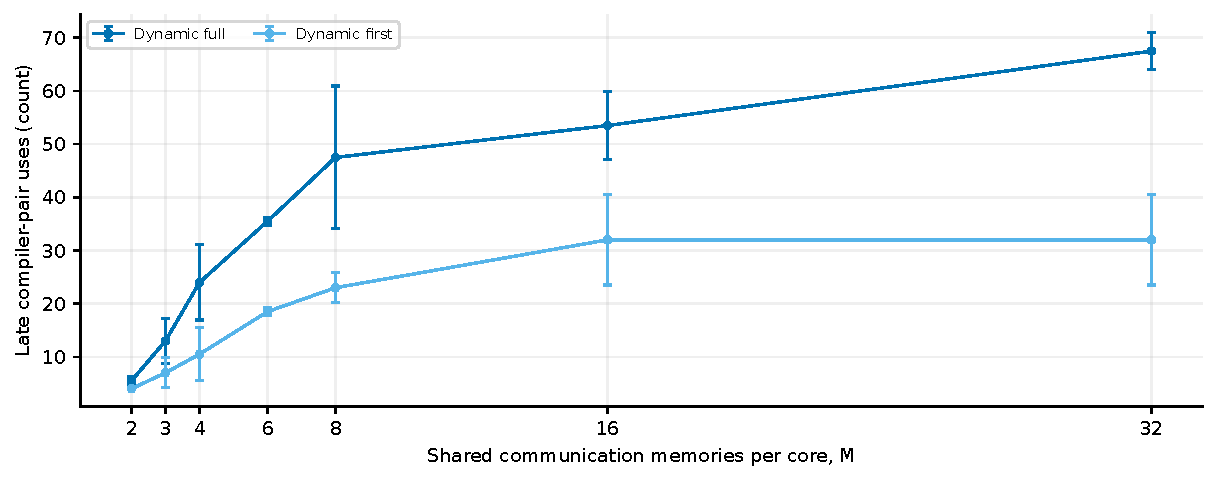
\includegraphics[width=.94\linewidth,height=.255\textheight,keepaspectratio]{figures/memory/mesh_yx_late_compiler_pair_uses.pdf}\captionof{figure}{Run-level mean and sample SD. Shared trace aliases are counted once.}\end{center}
\begin{center}{\scriptsize\setlength{\tabcolsep}{3pt}
\begin{tabular}{lrrrrr}
\toprule
M & ODG & CGP & ACGP & Dynamic full & Dynamic first \\
\midrule
2 & n/a & n/a & n/a & $5.500\pm0.707$ & $4.000\pm0.000$ \\
3 & n/a & n/a & n/a & $13.000\pm4.243$ & $7.000\pm2.828$ \\
4 & n/a & n/a & n/a & $24.000\pm7.071$ & $10.500\pm4.950$ \\
6 & n/a & n/a & n/a & $35.500\pm0.707$ & $18.500\pm0.707$ \\
8 & n/a & n/a & n/a & $47.500\pm13.435$ & $23.000\pm2.828$ \\
16 & n/a & n/a & n/a & $53.500\pm6.364$ & $32.000\pm8.485$ \\
32 & n/a & n/a & n/a & $67.500\pm3.536$ & $32.000\pm8.485$ \\
\bottomrule\end{tabular}}
\captionof{table}{Mean $\pm$ sample SD; n/a denotes a metric outside that policy's instrumentation.}
{\footnotesize\href{https://github.com/sanjeevkrishnaa/Compiler-Driven-ACE/blob/codex/ace-scheduler-correctness/docs/latex/qft96_final/data/memory_mesh_yx_late_compiler_pair_uses.csv}{Exact CSV values and sample counts}}
\end{center}
\subsection*{Compiler fallback count}
\begin{center}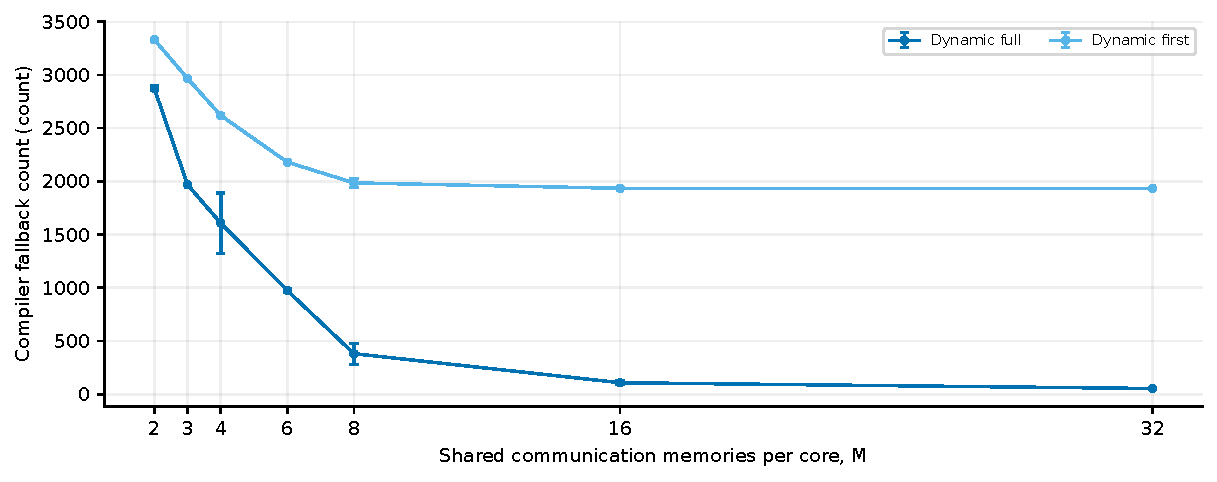
\includegraphics[width=.94\linewidth,height=.255\textheight,keepaspectratio]{figures/memory/mesh_yx_on_demand_fallbacks.pdf}\captionof{figure}{Run-level mean and sample SD. Shared trace aliases are counted once.}\end{center}
\begin{center}{\scriptsize\setlength{\tabcolsep}{3pt}
\begin{tabular}{lrrrrr}
\toprule
M & ODG & CGP & ACGP & Dynamic full & Dynamic first \\
\midrule
2 & n/a & n/a & n/a & $2874.00\pm24.04$ & $3330.00\pm9.90$ \\
3 & n/a & n/a & n/a & $1968.00\pm5.66$ & $2966.50\pm4.95$ \\
4 & n/a & n/a & n/a & $1606.00\pm284.26$ & $2618.00\pm2.83$ \\
6 & n/a & n/a & n/a & $973.50\pm16.26$ & $2179.50\pm16.26$ \\
8 & n/a & n/a & n/a & $381.00\pm98.99$ & $1985.50\pm40.31$ \\
16 & n/a & n/a & n/a & $108.00\pm16.97$ & $1934.00\pm4.24$ \\
32 & n/a & n/a & n/a & $53.500\pm4.950$ & $1934.00\pm4.24$ \\
\bottomrule\end{tabular}}
\captionof{table}{Mean $\pm$ sample SD; n/a denotes a metric outside that policy's instrumentation.}
{\footnotesize\href{https://github.com/sanjeevkrishnaa/Compiler-Driven-ACE/blob/codex/ace-scheduler-correctness/docs/latex/qft96_final/data/memory_mesh_yx_on_demand_fallbacks.csv}{Exact CSV values and sample counts}}
\end{center}
\clearpage
\subsection*{Generated compiler pairs}
\begin{center}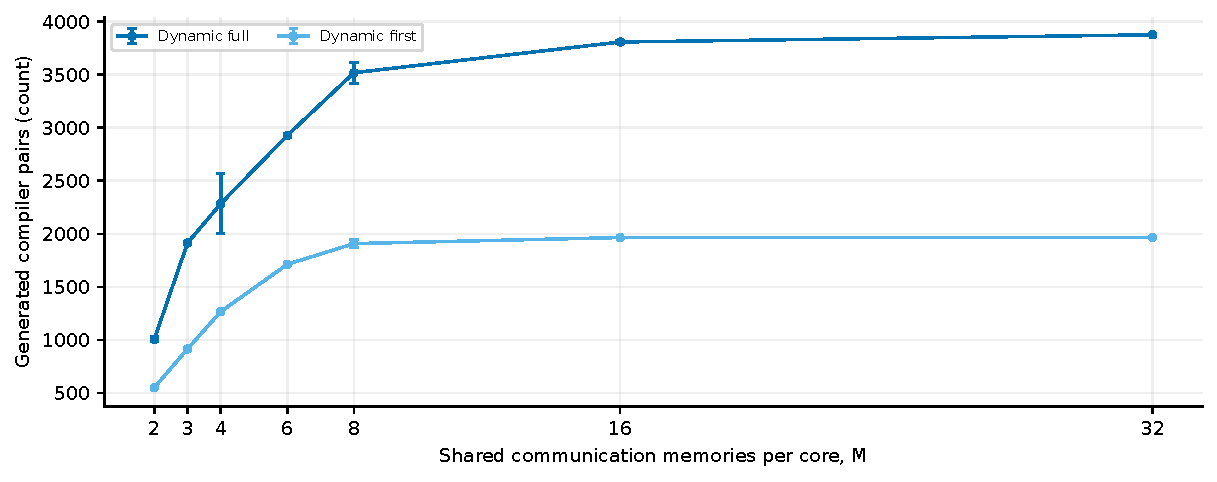
\includegraphics[width=.94\linewidth,height=.255\textheight,keepaspectratio]{figures/memory/mesh_yx_generated_compiler_pairs.pdf}\captionof{figure}{Run-level mean and sample SD. Shared trace aliases are counted once.}\end{center}
\begin{center}{\scriptsize\setlength{\tabcolsep}{3pt}
\begin{tabular}{lrrrrr}
\toprule
M & ODG & CGP & ACGP & Dynamic full & Dynamic first \\
\midrule
2 & n/a & n/a & n/a & $1005.00\pm24.04$ & $549.50\pm10.61$ \\
3 & n/a & n/a & n/a & $1914.00\pm7.07$ & $915.50\pm4.95$ \\
4 & n/a & n/a & n/a & $2285.00\pm280.01$ & $1267.00\pm2.83$ \\
6 & n/a & n/a & n/a & $2927.50\pm16.26$ & $1713.00\pm14.14$ \\
8 & n/a & n/a & n/a & $3518.50\pm99.70$ & $1908.00\pm36.77$ \\
16 & n/a & n/a & n/a & $3808.00\pm16.97$ & $1965.00\pm0.00$ \\
32 & n/a & n/a & n/a & $3876.00\pm0.00$ & $1965.00\pm0.00$ \\
\bottomrule\end{tabular}}
\captionof{table}{Mean $\pm$ sample SD; n/a denotes a metric outside that policy's instrumentation.}
{\footnotesize\href{https://github.com/sanjeevkrishnaa/Compiler-Driven-ACE/blob/codex/ace-scheduler-correctness/docs/latex/qft96_final/data/memory_mesh_yx_generated_compiler_pairs.csv}{Exact CSV values and sample counts}}
\end{center}
\subsection*{Used compiler pairs}
\begin{center}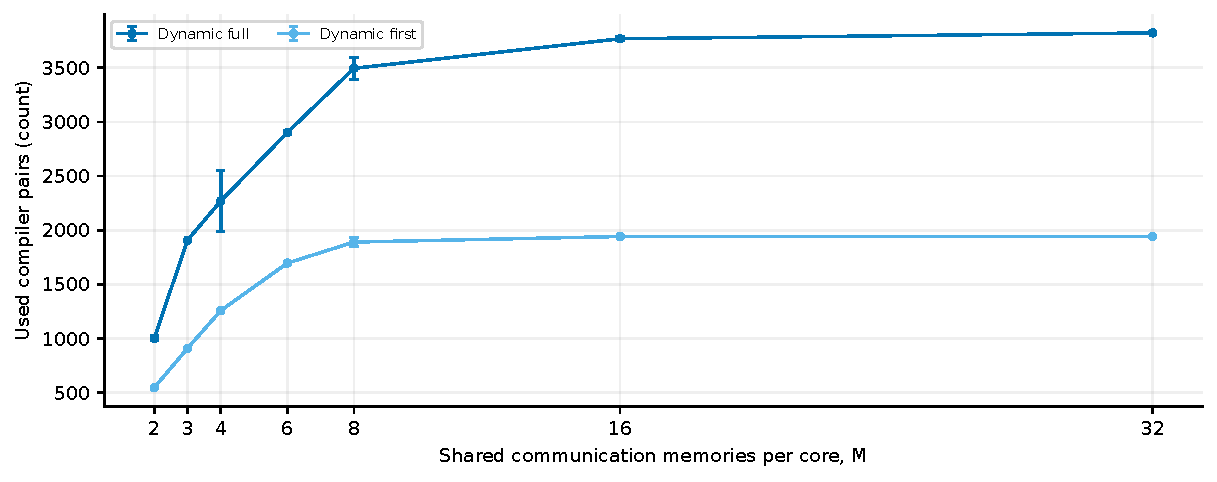
\includegraphics[width=.94\linewidth,height=.255\textheight,keepaspectratio]{figures/memory/mesh_yx_utilized_compiler_pairs.pdf}\captionof{figure}{Run-level mean and sample SD. Shared trace aliases are counted once.}\end{center}
\begin{center}{\scriptsize\setlength{\tabcolsep}{3pt}
\begin{tabular}{lrrrrr}
\toprule
M & ODG & CGP & ACGP & Dynamic full & Dynamic first \\
\midrule
2 & n/a & n/a & n/a & $1002.00\pm24.04$ & $546.00\pm9.90$ \\
3 & n/a & n/a & n/a & $1908.00\pm5.66$ & $909.50\pm4.95$ \\
4 & n/a & n/a & n/a & $2270.00\pm284.26$ & $1258.00\pm2.83$ \\
6 & n/a & n/a & n/a & $2902.50\pm16.26$ & $1696.50\pm16.26$ \\
8 & n/a & n/a & n/a & $3495.00\pm98.99$ & $1890.50\pm40.31$ \\
16 & n/a & n/a & n/a & $3768.00\pm16.97$ & $1942.00\pm4.24$ \\
32 & n/a & n/a & n/a & $3822.50\pm4.95$ & $1942.00\pm4.24$ \\
\bottomrule\end{tabular}}
\captionof{table}{Mean $\pm$ sample SD; n/a denotes a metric outside that policy's instrumentation.}
{\footnotesize\href{https://github.com/sanjeevkrishnaa/Compiler-Driven-ACE/blob/codex/ace-scheduler-correctness/docs/latex/qft96_final/data/memory_mesh_yx_utilized_compiler_pairs.csv}{Exact CSV values and sample counts}}
\end{center}
\clearpage
\subsection*{Expired compiler pairs}
\begin{center}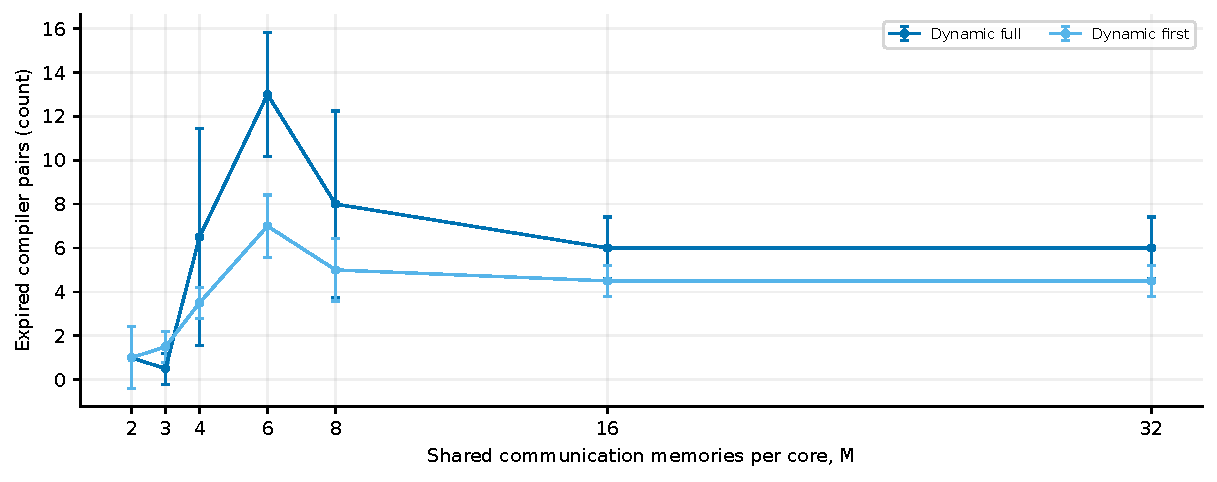
\includegraphics[width=.94\linewidth,height=.255\textheight,keepaspectratio]{figures/memory/mesh_yx_expired_compiler_pairs.pdf}\captionof{figure}{Run-level mean and sample SD. Shared trace aliases are counted once.}\end{center}
\begin{center}{\scriptsize\setlength{\tabcolsep}{3pt}
\begin{tabular}{lrrrrr}
\toprule
M & ODG & CGP & ACGP & Dynamic full & Dynamic first \\
\midrule
2 & n/a & n/a & n/a & $1.000\pm1.414$ & $1.000\pm1.414$ \\
3 & n/a & n/a & n/a & $0.5000\pm0.7071$ & $1.500\pm0.707$ \\
4 & n/a & n/a & n/a & $6.500\pm4.950$ & $3.500\pm0.707$ \\
6 & n/a & n/a & n/a & $13.000\pm2.828$ & $7.000\pm1.414$ \\
8 & n/a & n/a & n/a & $8.000\pm4.243$ & $5.000\pm1.414$ \\
16 & n/a & n/a & n/a & $6.000\pm1.414$ & $4.500\pm0.707$ \\
32 & n/a & n/a & n/a & $6.000\pm1.414$ & $4.500\pm0.707$ \\
\bottomrule\end{tabular}}
\captionof{table}{Mean $\pm$ sample SD; n/a denotes a metric outside that policy's instrumentation.}
{\footnotesize\href{https://github.com/sanjeevkrishnaa/Compiler-Driven-ACE/blob/codex/ace-scheduler-correctness/docs/latex/qft96_final/data/memory_mesh_yx_expired_compiler_pairs.csv}{Exact CSV values and sample counts}}
\end{center}
\subsection*{Remaining compiler pairs}
\begin{center}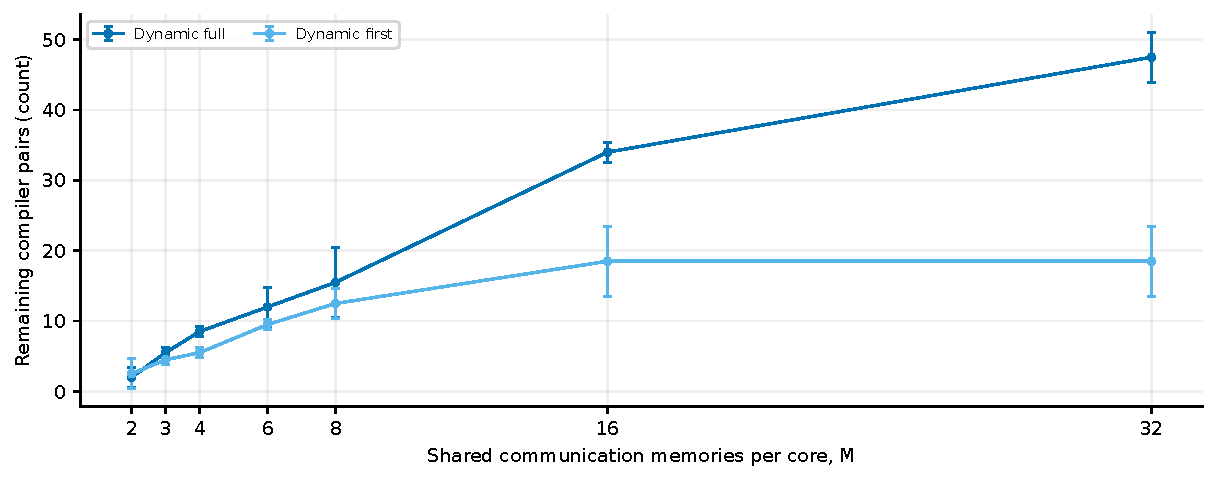
\includegraphics[width=.94\linewidth,height=.255\textheight,keepaspectratio]{figures/memory/mesh_yx_remaining_compiler_pairs.pdf}\captionof{figure}{Run-level mean and sample SD. Shared trace aliases are counted once.}\end{center}
\begin{center}{\scriptsize\setlength{\tabcolsep}{3pt}
\begin{tabular}{lrrrrr}
\toprule
M & ODG & CGP & ACGP & Dynamic full & Dynamic first \\
\midrule
2 & n/a & n/a & n/a & $2.000\pm1.414$ & $2.500\pm2.121$ \\
3 & n/a & n/a & n/a & $5.500\pm0.707$ & $4.500\pm0.707$ \\
4 & n/a & n/a & n/a & $8.500\pm0.707$ & $5.500\pm0.707$ \\
6 & n/a & n/a & n/a & $12.000\pm2.828$ & $9.500\pm0.707$ \\
8 & n/a & n/a & n/a & $15.500\pm4.950$ & $12.500\pm2.121$ \\
16 & n/a & n/a & n/a & $34.000\pm1.414$ & $18.500\pm4.950$ \\
32 & n/a & n/a & n/a & $47.500\pm3.536$ & $18.500\pm4.950$ \\
\bottomrule\end{tabular}}
\captionof{table}{Mean $\pm$ sample SD; n/a denotes a metric outside that policy's instrumentation.}
{\footnotesize\href{https://github.com/sanjeevkrishnaa/Compiler-Driven-ACE/blob/codex/ace-scheduler-correctness/docs/latex/qft96_final/data/memory_mesh_yx_remaining_compiler_pairs.csv}{Exact CSV values and sample counts}}
\end{center}
\clearpage
\subsection*{Compiler fidelity at creation}
\begin{center}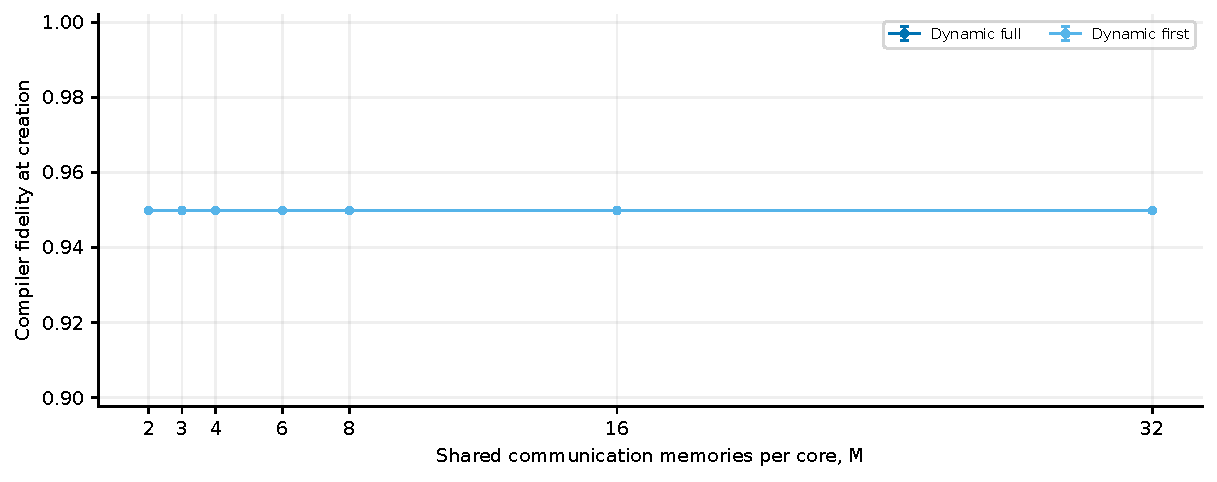
\includegraphics[width=.94\linewidth,height=.255\textheight,keepaspectratio]{figures/memory/mesh_yx_average_fidelity_at_creation.pdf}\captionof{figure}{Run-level mean and sample SD. Shared trace aliases are counted once.}\end{center}
\begin{center}{\scriptsize\setlength{\tabcolsep}{3pt}
\begin{tabular}{lrrrrr}
\toprule
M & ODG & CGP & ACGP & Dynamic full & Dynamic first \\
\midrule
2 & n/a & n/a & n/a & $0.9498\pm0.0000$ & $0.9498\pm0.0000$ \\
3 & n/a & n/a & n/a & $0.9498\pm0.0000$ & $0.9498\pm0.0000$ \\
4 & n/a & n/a & n/a & $0.9498\pm0.0000$ & $0.9498\pm0.0000$ \\
6 & n/a & n/a & n/a & $0.9498\pm0.0000$ & $0.9498\pm0.0000$ \\
8 & n/a & n/a & n/a & $0.9498\pm0.0000$ & $0.9498\pm0.0000$ \\
16 & n/a & n/a & n/a & $0.9498\pm0.0000$ & $0.9498\pm0.0000$ \\
32 & n/a & n/a & n/a & $0.9498\pm0.0000$ & $0.9498\pm0.0000$ \\
\bottomrule\end{tabular}}
\captionof{table}{Mean $\pm$ sample SD; n/a denotes a metric outside that policy's instrumentation.}
{\footnotesize\href{https://github.com/sanjeevkrishnaa/Compiler-Driven-ACE/blob/codex/ace-scheduler-correctness/docs/latex/qft96_final/data/memory_mesh_yx_average_fidelity_at_creation.csv}{Exact CSV values and sample counts}}
\end{center}
\subsection*{Compiler fidelity at use}
\begin{center}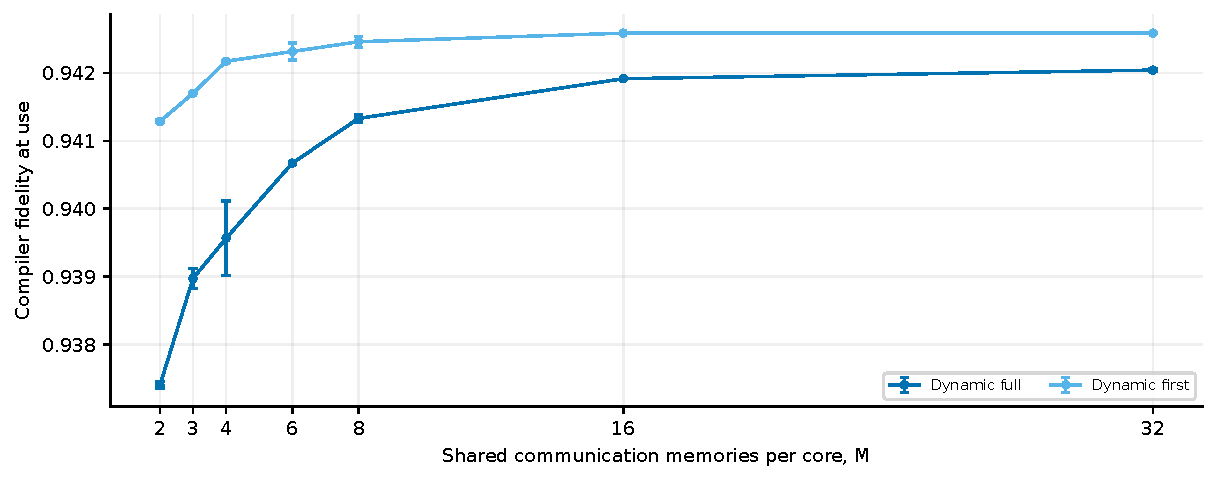
\includegraphics[width=.94\linewidth,height=.255\textheight,keepaspectratio]{figures/memory/mesh_yx_average_fidelity_at_utilization.pdf}\captionof{figure}{Run-level mean and sample SD. Shared trace aliases are counted once.}\end{center}
\begin{center}{\scriptsize\setlength{\tabcolsep}{3pt}
\begin{tabular}{lrrrrr}
\toprule
M & ODG & CGP & ACGP & Dynamic full & Dynamic first \\
\midrule
2 & n/a & n/a & n/a & $0.9374\pm0.0001$ & $0.9413\pm0.0000$ \\
3 & n/a & n/a & n/a & $0.9390\pm0.0001$ & $0.9417\pm0.0000$ \\
4 & n/a & n/a & n/a & $0.9396\pm0.0005$ & $0.9422\pm0.0000$ \\
6 & n/a & n/a & n/a & $0.9407\pm0.0000$ & $0.9423\pm0.0001$ \\
8 & n/a & n/a & n/a & $0.9413\pm0.0001$ & $0.9425\pm0.0001$ \\
16 & n/a & n/a & n/a & $0.9419\pm0.0000$ & $0.9426\pm0.0000$ \\
32 & n/a & n/a & n/a & $0.9420\pm0.0000$ & $0.9426\pm0.0000$ \\
\bottomrule\end{tabular}}
\captionof{table}{Mean $\pm$ sample SD; n/a denotes a metric outside that policy's instrumentation.}
{\footnotesize\href{https://github.com/sanjeevkrishnaa/Compiler-Driven-ACE/blob/codex/ace-scheduler-correctness/docs/latex/qft96_final/data/memory_mesh_yx_average_fidelity_at_utilization.csv}{Exact CSV values and sample counts}}
\end{center}
\clearpage
\subsection*{Mean layer latency}
\begin{center}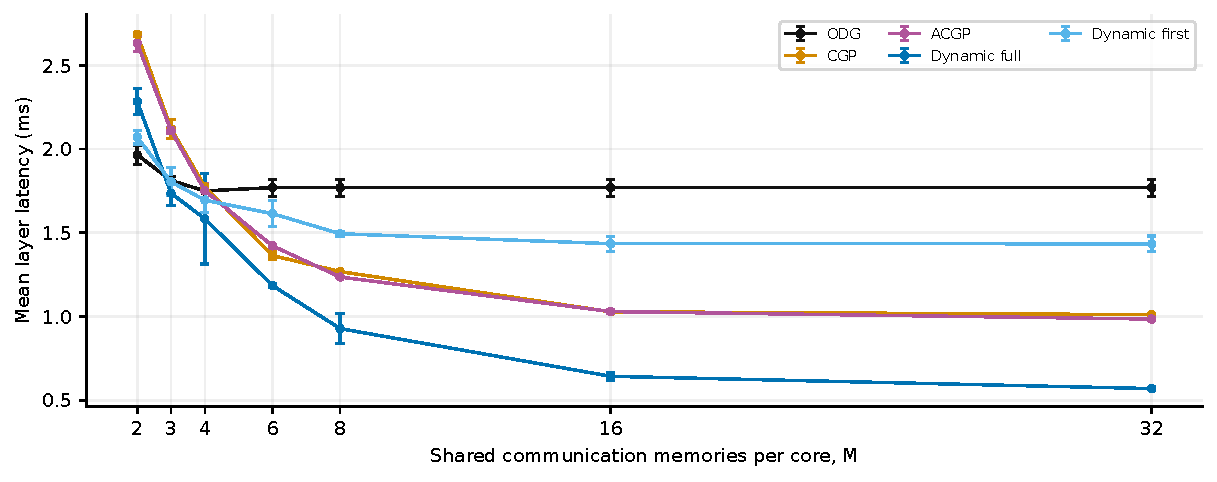
\includegraphics[width=.94\linewidth,height=.255\textheight,keepaspectratio]{figures/memory/mesh_yx_avg_layer_latency_ms.pdf}\captionof{figure}{Run-level mean and sample SD. Shared trace aliases are counted once.}\end{center}
\begin{center}{\scriptsize\setlength{\tabcolsep}{3pt}
\begin{tabular}{lrrrrr}
\toprule
M & ODG & CGP & ACGP & Dynamic full & Dynamic first \\
\midrule
2 & $1.966\pm0.057$ & $2.686\pm0.012$ & $2.632\pm0.047$ & $2.284\pm0.076$ & $2.072\pm0.042$ \\
3 & $1.812\pm0.023$ & $2.122\pm0.057$ & $2.111\pm0.017$ & $1.737\pm0.071$ & $1.805\pm0.084$ \\
4 & $1.750\pm0.042$ & $1.776\pm0.008$ & $1.751\pm0.042$ & $1.584\pm0.270$ & $1.695\pm0.076$ \\
6 & $1.770\pm0.051$ & $1.364\pm0.024$ & $1.422\pm0.008$ & $1.185\pm0.011$ & $1.614\pm0.078$ \\
8 & $1.770\pm0.051$ & $1.268\pm0.003$ & $1.236\pm0.005$ & $0.9278\pm0.0912$ & $1.495\pm0.014$ \\
16 & $1.770\pm0.051$ & $1.029\pm0.002$ & $1.029\pm0.010$ & $0.6428\pm0.0220$ & $1.435\pm0.046$ \\
32 & $1.770\pm0.051$ & $1.011\pm0.008$ & $0.9847\pm0.0091$ & $0.5693\pm0.0008$ & $1.434\pm0.046$ \\
\bottomrule\end{tabular}}
\captionof{table}{Mean $\pm$ sample SD; n/a denotes a metric outside that policy's instrumentation.}
{\footnotesize\href{https://github.com/sanjeevkrishnaa/Compiler-Driven-ACE/blob/codex/ace-scheduler-correctness/docs/latex/qft96_final/data/memory_mesh_yx_avg_layer_latency_ms.csv}{Exact CSV values and sample counts}}
\end{center}
\subsection*{Maximum layer latency}
\begin{center}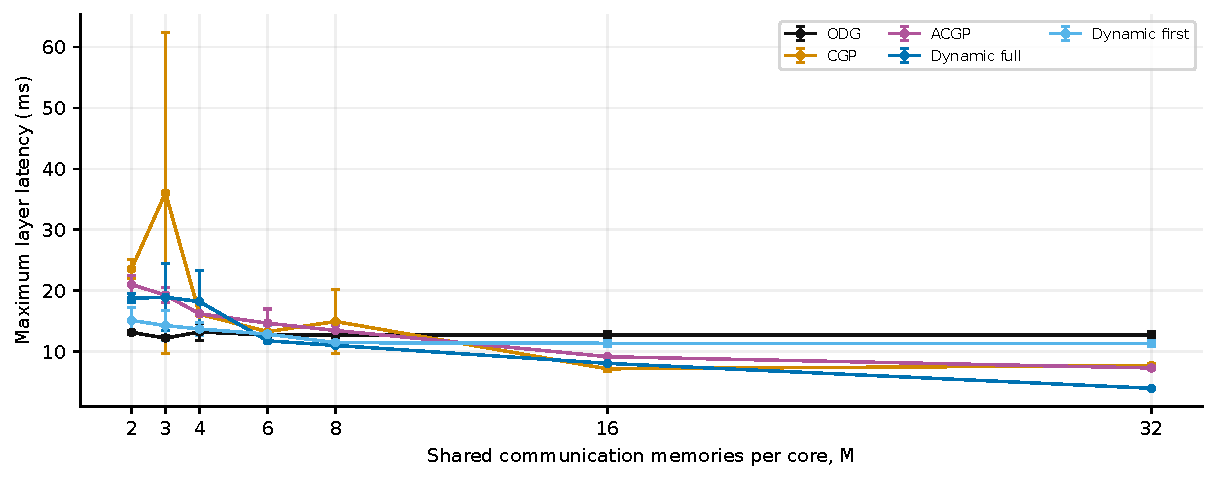
\includegraphics[width=.94\linewidth,height=.255\textheight,keepaspectratio]{figures/memory/mesh_yx_max_layer_latency_ms.pdf}\captionof{figure}{Run-level mean and sample SD. Shared trace aliases are counted once.}\end{center}
\begin{center}{\scriptsize\setlength{\tabcolsep}{3pt}
\begin{tabular}{lrrrrr}
\toprule
M & ODG & CGP & ACGP & Dynamic full & Dynamic first \\
\midrule
2 & $13.150\pm0.354$ & $23.551\pm1.626$ & $21.000\pm1.414$ & $18.750\pm0.778$ & $15.100\pm2.121$ \\
3 & $12.200\pm0.424$ & $36.050\pm26.375$ & $19.250\pm1.202$ & $18.900\pm5.516$ & $14.250\pm2.475$ \\
4 & $13.200\pm1.414$ & $16.150\pm0.212$ & $16.200\pm0.141$ & $18.200\pm5.091$ & $13.700\pm0.990$ \\
6 & $12.700\pm0.566$ & $13.250\pm0.212$ & $14.650\pm2.333$ & $11.750\pm0.212$ & $12.850\pm1.344$ \\
8 & $12.700\pm0.566$ & $14.932\pm5.188$ & $13.450\pm0.778$ & $11.000\pm0.141$ & $11.450\pm0.354$ \\
16 & $12.700\pm0.566$ & $7.150\pm0.495$ & $9.143\pm0.202$ & $8.050\pm1.202$ & $11.350\pm0.495$ \\
32 & $12.700\pm0.566$ & $7.700\pm0.283$ & $7.289\pm0.298$ & $3.950\pm0.071$ & $11.350\pm0.495$ \\
\bottomrule\end{tabular}}
\captionof{table}{Mean $\pm$ sample SD; n/a denotes a metric outside that policy's instrumentation.}
{\footnotesize\href{https://github.com/sanjeevkrishnaa/Compiler-Driven-ACE/blob/codex/ace-scheduler-correctness/docs/latex/qft96_final/data/memory_mesh_yx_max_layer_latency_ms.csv}{Exact CSV values and sample counts}}
\end{center}
\clearpage
\subsection*{Minimum layer latency}
\begin{center}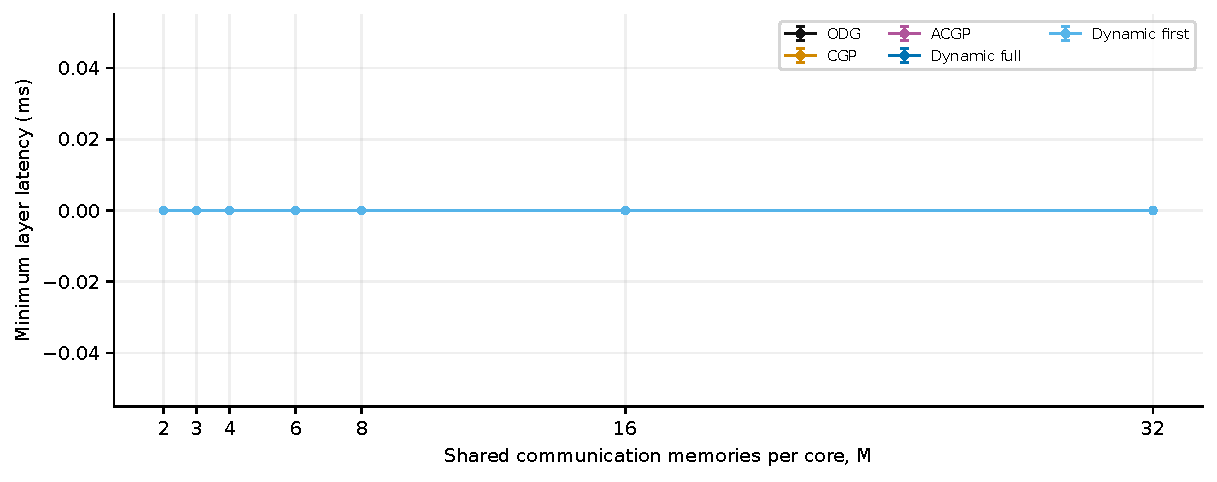
\includegraphics[width=.94\linewidth,height=.255\textheight,keepaspectratio]{figures/memory/mesh_yx_min_layer_latency_ms.pdf}\captionof{figure}{Run-level mean and sample SD. Shared trace aliases are counted once.}\end{center}
\begin{center}{\scriptsize\setlength{\tabcolsep}{3pt}
\begin{tabular}{lrrrrr}
\toprule
M & ODG & CGP & ACGP & Dynamic full & Dynamic first \\
\midrule
2 & $0.0000\pm0.0000$ & $0.0000\pm0.0000$ & $0.0000\pm0.0000$ & $0.0000\pm0.0000$ & $0.0000\pm0.0000$ \\
3 & $0.0000\pm0.0000$ & $0.0000\pm0.0000$ & $0.0000\pm0.0000$ & $0.0000\pm0.0000$ & $0.0000\pm0.0000$ \\
4 & $0.0000\pm0.0000$ & $0.0000\pm0.0000$ & $0.0000\pm0.0000$ & $0.0000\pm0.0000$ & $0.0000\pm0.0000$ \\
6 & $0.0000\pm0.0000$ & $0.0000\pm0.0000$ & $0.0000\pm0.0000$ & $0.0000\pm0.0000$ & $0.0000\pm0.0000$ \\
8 & $0.0000\pm0.0000$ & $0.0000\pm0.0000$ & $0.0000\pm0.0000$ & $0.0000\pm0.0000$ & $0.0000\pm0.0000$ \\
16 & $0.0000\pm0.0000$ & $0.0000\pm0.0000$ & $0.0000\pm0.0000$ & $0.0000\pm0.0000$ & $0.0000\pm0.0000$ \\
32 & $0.0000\pm0.0000$ & $0.0000\pm0.0000$ & $0.0000\pm0.0000$ & $0.0000\pm0.0000$ & $0.0000\pm0.0000$ \\
\bottomrule\end{tabular}}
\captionof{table}{Mean $\pm$ sample SD; n/a denotes a metric outside that policy's instrumentation.}
{\footnotesize\href{https://github.com/sanjeevkrishnaa/Compiler-Driven-ACE/blob/codex/ace-scheduler-correctness/docs/latex/qft96_final/data/memory_mesh_yx_min_layer_latency_ms.csv}{Exact CSV values and sample counts}}
\end{center}
\section{Shortest Reliable}
\clearpage
\subsection*{Mean request latency}
\begin{center}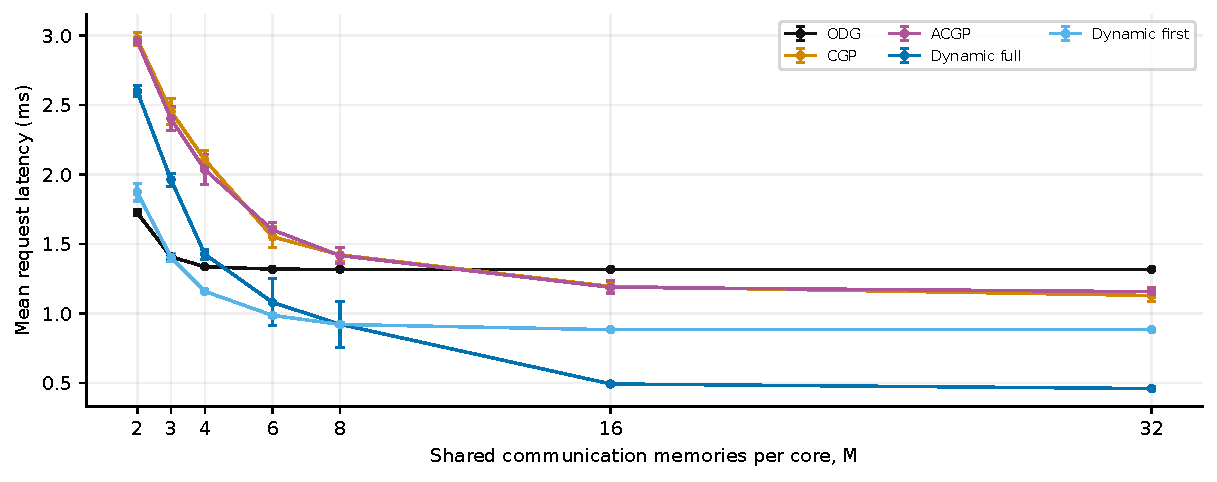
\includegraphics[width=.94\linewidth,height=.255\textheight,keepaspectratio]{figures/memory/mesh_shortest_reliable_request_latency_mean_ms.pdf}\captionof{figure}{Run-level mean and sample SD. Shared trace aliases are counted once.}\end{center}
\begin{center}{\scriptsize\setlength{\tabcolsep}{3pt}
\begin{tabular}{lrrrrr}
\toprule
M & ODG & CGP & ACGP & Dynamic full & Dynamic first \\
\midrule
2 & $1.726\pm0.022$ & $2.976\pm0.047$ & $2.959\pm0.027$ & $2.598\pm0.040$ & $1.872\pm0.062$ \\
3 & $1.408\pm0.010$ & $2.455\pm0.093$ & $2.401\pm0.085$ & $1.963\pm0.046$ & $1.405\pm0.028$ \\
4 & $1.337\pm0.005$ & $2.106\pm0.066$ & $2.035\pm0.109$ & $1.427\pm0.036$ & $1.160\pm0.010$ \\
6 & $1.319\pm0.004$ & $1.553\pm0.077$ & $1.602\pm0.053$ & $1.080\pm0.169$ & $0.9875\pm0.0125$ \\
8 & $1.319\pm0.004$ & $1.422\pm0.051$ & $1.417\pm0.059$ & $0.9230\pm0.1635$ & $0.9220\pm0.0102$ \\
16 & $1.318\pm0.004$ & $1.195\pm0.043$ & $1.189\pm0.046$ & $0.4941\pm0.0101$ & $0.8841\pm0.0083$ \\
32 & $1.318\pm0.004$ & $1.130\pm0.046$ & $1.157\pm0.030$ & $0.4607\pm0.0011$ & $0.8841\pm0.0083$ \\
\bottomrule\end{tabular}}
\captionof{table}{Mean $\pm$ sample SD; n/a denotes a metric outside that policy's instrumentation.}
{\footnotesize\href{https://github.com/sanjeevkrishnaa/Compiler-Driven-ACE/blob/codex/ace-scheduler-correctness/docs/latex/qft96_final/data/memory_mesh_shortest_reliable_request_latency_mean_ms.csv}{Exact CSV values and sample counts}}
\end{center}
\subsection*{Median request latency}
\begin{center}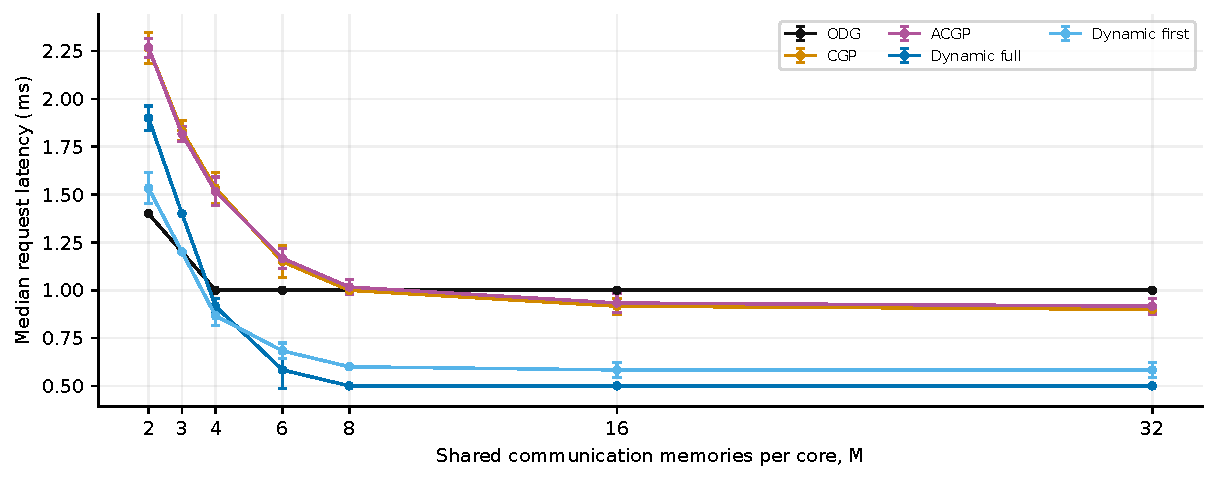
\includegraphics[width=.94\linewidth,height=.255\textheight,keepaspectratio]{figures/memory/mesh_shortest_reliable_request_latency_median_ms.pdf}\captionof{figure}{Run-level mean and sample SD. Shared trace aliases are counted once.}\end{center}
\begin{center}{\scriptsize\setlength{\tabcolsep}{3pt}
\begin{tabular}{lrrrrr}
\toprule
M & ODG & CGP & ACGP & Dynamic full & Dynamic first \\
\midrule
2 & $1.400\pm0.000$ & $2.267\pm0.082$ & $2.268\pm0.050$ & $1.900\pm0.063$ & $1.533\pm0.082$ \\
3 & $1.200\pm0.000$ & $1.833\pm0.052$ & $1.817\pm0.041$ & $1.400\pm0.000$ & $1.200\pm0.000$ \\
4 & $1.000\pm0.000$ & $1.533\pm0.082$ & $1.517\pm0.075$ & $0.9167\pm0.0408$ & $0.8667\pm0.0516$ \\
6 & $1.000\pm0.000$ & $1.150\pm0.084$ & $1.167\pm0.052$ & $0.5833\pm0.0983$ & $0.6833\pm0.0408$ \\
8 & $1.000\pm0.000$ & $1.000\pm0.000$ & $1.017\pm0.041$ & $0.5000\pm0.0000$ & $0.6000\pm0.0000$ \\
16 & $1.000\pm0.000$ & $0.9167\pm0.0408$ & $0.9333\pm0.0516$ & $0.5000\pm0.0000$ & $0.5833\pm0.0408$ \\
32 & $1.000\pm0.000$ & $0.9000\pm0.0000$ & $0.9167\pm0.0408$ & $0.5000\pm0.0000$ & $0.5833\pm0.0408$ \\
\bottomrule\end{tabular}}
\captionof{table}{Mean $\pm$ sample SD; n/a denotes a metric outside that policy's instrumentation.}
{\footnotesize\href{https://github.com/sanjeevkrishnaa/Compiler-Driven-ACE/blob/codex/ace-scheduler-correctness/docs/latex/qft96_final/data/memory_mesh_shortest_reliable_request_latency_median_ms.csv}{Exact CSV values and sample counts}}
\end{center}
\clearpage
\subsection*{p95 request latency}
\begin{center}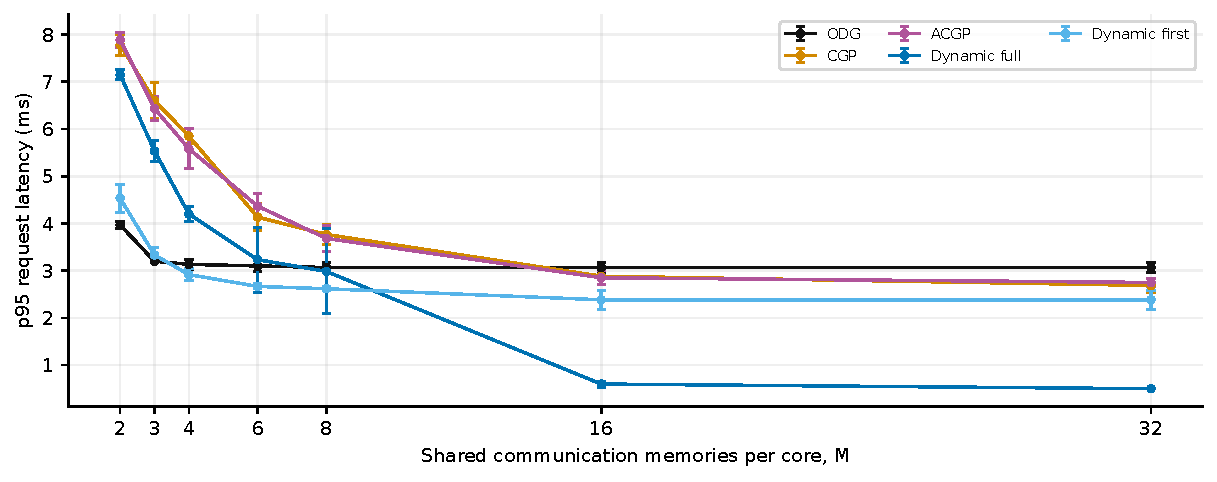
\includegraphics[width=.94\linewidth,height=.255\textheight,keepaspectratio]{figures/memory/mesh_shortest_reliable_request_latency_p95_ms.pdf}\captionof{figure}{Run-level mean and sample SD. Shared trace aliases are counted once.}\end{center}
\begin{center}{\scriptsize\setlength{\tabcolsep}{3pt}
\begin{tabular}{lrrrrr}
\toprule
M & ODG & CGP & ACGP & Dynamic full & Dynamic first \\
\midrule
2 & $3.967\pm0.082$ & $7.785\pm0.226$ & $7.886\pm0.161$ & $7.150\pm0.105$ & $4.533\pm0.294$ \\
3 & $3.200\pm0.000$ & $6.600\pm0.385$ & $6.433\pm0.258$ & $5.533\pm0.225$ & $3.333\pm0.163$ \\
4 & $3.133\pm0.103$ & $5.850\pm0.164$ & $5.581\pm0.424$ & $4.200\pm0.155$ & $2.917\pm0.133$ \\
6 & $3.100\pm0.110$ & $4.133\pm0.288$ & $4.367\pm0.258$ & $3.233\pm0.689$ & $2.667\pm0.052$ \\
8 & $3.067\pm0.103$ & $3.767\pm0.216$ & $3.683\pm0.279$ & $2.983\pm0.900$ & $2.617\pm0.041$ \\
16 & $3.067\pm0.103$ & $2.883\pm0.172$ & $2.850\pm0.152$ & $0.6000\pm0.0633$ & $2.383\pm0.204$ \\
32 & $3.067\pm0.103$ & $2.687\pm0.150$ & $2.750\pm0.084$ & $0.5000\pm0.0000$ & $2.383\pm0.204$ \\
\bottomrule\end{tabular}}
\captionof{table}{Mean $\pm$ sample SD; n/a denotes a metric outside that policy's instrumentation.}
{\footnotesize\href{https://github.com/sanjeevkrishnaa/Compiler-Driven-ACE/blob/codex/ace-scheduler-correctness/docs/latex/qft96_final/data/memory_mesh_shortest_reliable_request_latency_p95_ms.csv}{Exact CSV values and sample counts}}
\end{center}
\subsection*{Maximum request latency}
\begin{center}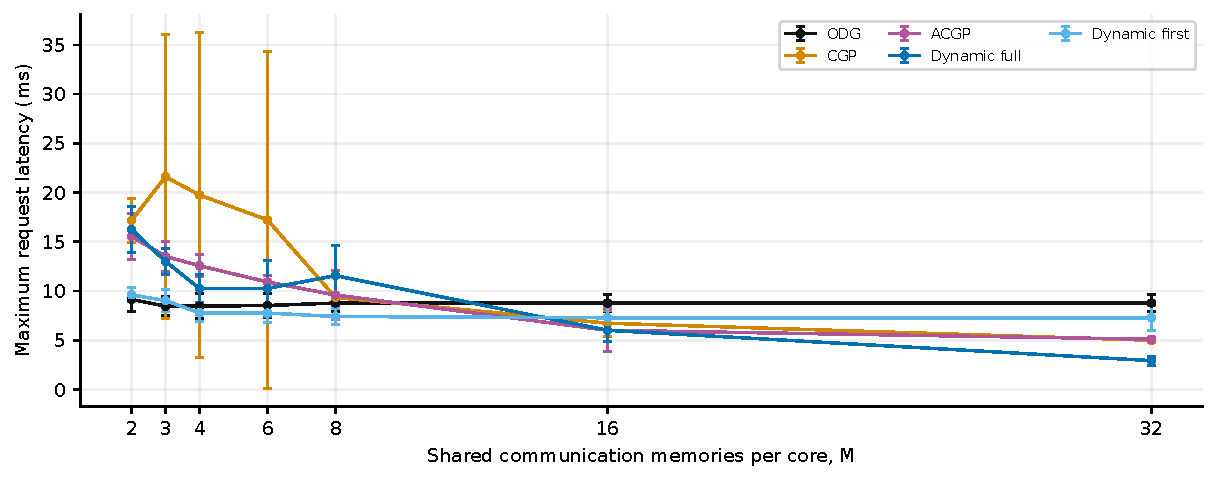
\includegraphics[width=.94\linewidth,height=.255\textheight,keepaspectratio]{figures/memory/mesh_shortest_reliable_request_latency_max_ms.pdf}\captionof{figure}{Run-level mean and sample SD. Shared trace aliases are counted once.}\end{center}
\begin{center}{\scriptsize\setlength{\tabcolsep}{3pt}
\begin{tabular}{lrrrrr}
\toprule
M & ODG & CGP & ACGP & Dynamic full & Dynamic first \\
\midrule
2 & $9.150\pm1.190$ & $17.166\pm2.216$ & $15.550\pm2.321$ & $16.250\pm2.318$ & $9.617\pm0.697$ \\
3 & $8.467\pm0.965$ & $21.600\pm14.422$ & $13.517\pm1.515$ & $13.017\pm1.332$ & $9.034\pm1.129$ \\
4 & $8.467\pm1.244$ & $19.750\pm16.521$ & $12.567\pm1.111$ & $10.250\pm1.429$ & $7.784\pm0.911$ \\
6 & $8.534\pm1.211$ & $17.224\pm17.144$ & $10.917\pm0.697$ & $10.267\pm2.813$ & $7.767\pm0.973$ \\
8 & $8.784\pm0.861$ & $9.347\pm2.058$ & $9.602\pm2.462$ & $11.567\pm3.089$ & $7.417\pm0.809$ \\
16 & $8.784\pm0.861$ & $6.733\pm1.332$ & $6.017\pm2.181$ & $6.017\pm1.155$ & $7.284\pm1.298$ \\
32 & $8.784\pm0.861$ & $5.000\pm0.179$ & $5.107\pm0.175$ & $2.933\pm0.463$ & $7.284\pm1.298$ \\
\bottomrule\end{tabular}}
\captionof{table}{Mean $\pm$ sample SD; n/a denotes a metric outside that policy's instrumentation.}
{\footnotesize\href{https://github.com/sanjeevkrishnaa/Compiler-Driven-ACE/blob/codex/ace-scheduler-correctness/docs/latex/qft96_final/data/memory_mesh_shortest_reliable_request_latency_max_ms.csv}{Exact CSV values and sample counts}}
\end{center}
\clearpage
\subsection*{Communication makespan}
\begin{center}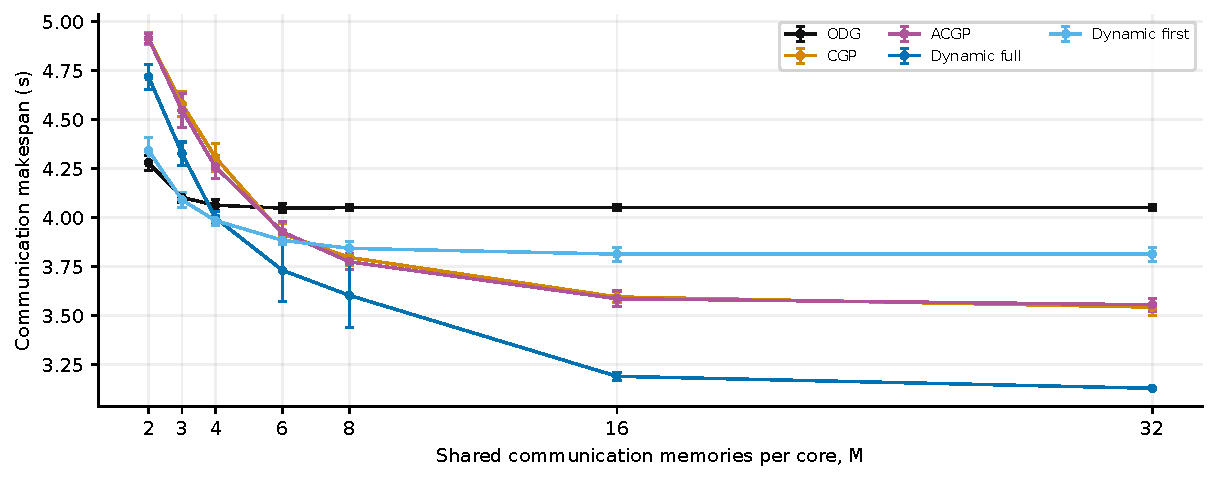
\includegraphics[width=.94\linewidth,height=.255\textheight,keepaspectratio]{figures/memory/mesh_shortest_reliable_end_to_end_latency_ms.pdf}\captionof{figure}{Run-level mean and sample SD. Shared trace aliases are counted once.}\end{center}
\begin{center}{\scriptsize\setlength{\tabcolsep}{3pt}
\begin{tabular}{lrrrrr}
\toprule
M & ODG & CGP & ACGP & Dynamic full & Dynamic first \\
\midrule
2 & $4.280\pm0.038$ & $4.914\pm0.031$ & $4.914\pm0.025$ & $4.718\pm0.063$ & $4.342\pm0.064$ \\
3 & $4.103\pm0.026$ & $4.580\pm0.065$ & $4.548\pm0.086$ & $4.327\pm0.059$ & $4.090\pm0.039$ \\
4 & $4.064\pm0.029$ & $4.307\pm0.070$ & $4.258\pm0.060$ & $3.998\pm0.031$ & $3.985\pm0.026$ \\
6 & $4.049\pm0.021$ & $3.917\pm0.052$ & $3.927\pm0.053$ & $3.731\pm0.161$ & $3.885\pm0.024$ \\
8 & $4.051\pm0.017$ & $3.797\pm0.039$ & $3.775\pm0.041$ & $3.604\pm0.165$ & $3.843\pm0.035$ \\
16 & $4.051\pm0.017$ & $3.596\pm0.030$ & $3.586\pm0.039$ & $3.191\pm0.019$ & $3.814\pm0.035$ \\
32 & $4.051\pm0.017$ & $3.543\pm0.043$ & $3.555\pm0.033$ & $3.129\pm0.002$ & $3.814\pm0.035$ \\
\bottomrule\end{tabular}}
\captionof{table}{Mean $\pm$ sample SD; n/a denotes a metric outside that policy's instrumentation.}
{\footnotesize\href{https://github.com/sanjeevkrishnaa/Compiler-Driven-ACE/blob/codex/ace-scheduler-correctness/docs/latex/qft96_final/data/memory_mesh_shortest_reliable_end_to_end_latency_ms.csv}{Exact CSV values and sample counts}}
\end{center}
\subsection*{Mean admission wait}
\begin{center}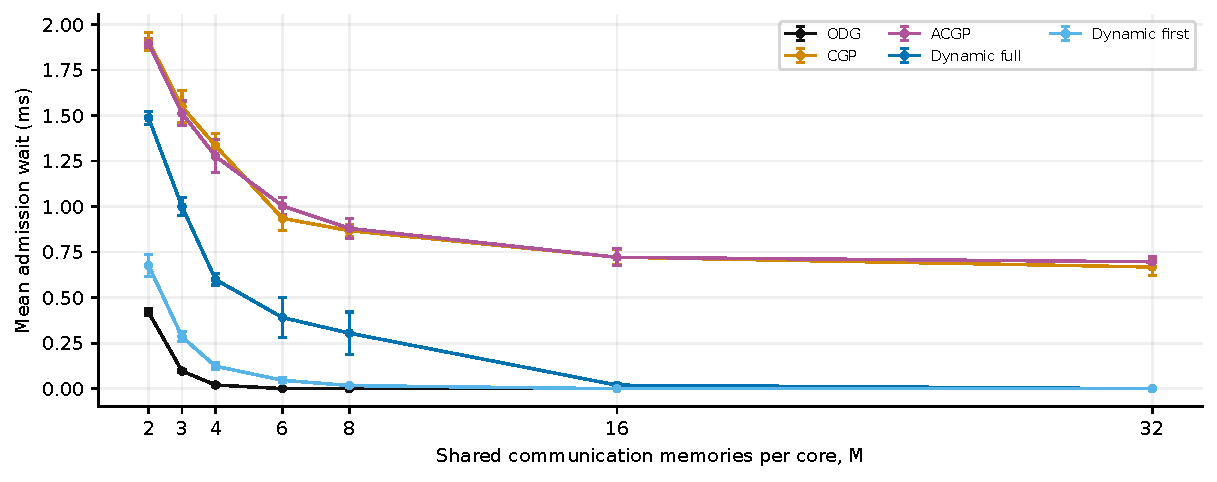
\includegraphics[width=.94\linewidth,height=.255\textheight,keepaspectratio]{figures/memory/mesh_shortest_reliable_average_admission_wait_ms.pdf}\captionof{figure}{Run-level mean and sample SD. Shared trace aliases are counted once.}\end{center}
\begin{center}{\scriptsize\setlength{\tabcolsep}{3pt}
\begin{tabular}{lrrrrr}
\toprule
M & ODG & CGP & ACGP & Dynamic full & Dynamic first \\
\midrule
2 & $0.4199\pm0.0197$ & $1.907\pm0.050$ & $1.896\pm0.024$ & $1.487\pm0.035$ & $0.6768\pm0.0582$ \\
3 & $0.0969\pm0.0073$ & $1.549\pm0.087$ & $1.513\pm0.067$ & $0.9992\pm0.0485$ & $0.2847\pm0.0275$ \\
4 & $0.0205\pm0.0007$ & $1.335\pm0.065$ & $1.277\pm0.090$ & $0.6000\pm0.0306$ & $0.1238\pm0.0192$ \\
6 & $0.0007\pm0.0006$ & $0.9356\pm0.0657$ & $1.004\pm0.047$ & $0.3909\pm0.1095$ & $0.0466\pm0.0122$ \\
8 & $0.0000\pm0.0001$ & $0.8681\pm0.0341$ & $0.8804\pm0.0532$ & $0.3053\pm0.1160$ & $0.0174\pm0.0073$ \\
16 & $0.0000\pm0.0000$ & $0.7223\pm0.0410$ & $0.7215\pm0.0467$ & $0.0196\pm0.0071$ & $0.0000\pm0.0000$ \\
32 & $0.0000\pm0.0000$ & $0.6681\pm0.0480$ & $0.6969\pm0.0310$ & $0.0000\pm0.0000$ & $0.0000\pm0.0000$ \\
\bottomrule\end{tabular}}
\captionof{table}{Mean $\pm$ sample SD; n/a denotes a metric outside that policy's instrumentation.}
{\footnotesize\href{https://github.com/sanjeevkrishnaa/Compiler-Driven-ACE/blob/codex/ace-scheduler-correctness/docs/latex/qft96_final/data/memory_mesh_shortest_reliable_average_admission_wait_ms.csv}{Exact CSV values and sample counts}}
\end{center}
\clearpage
\subsection*{Delivered EPR fidelity}
\begin{center}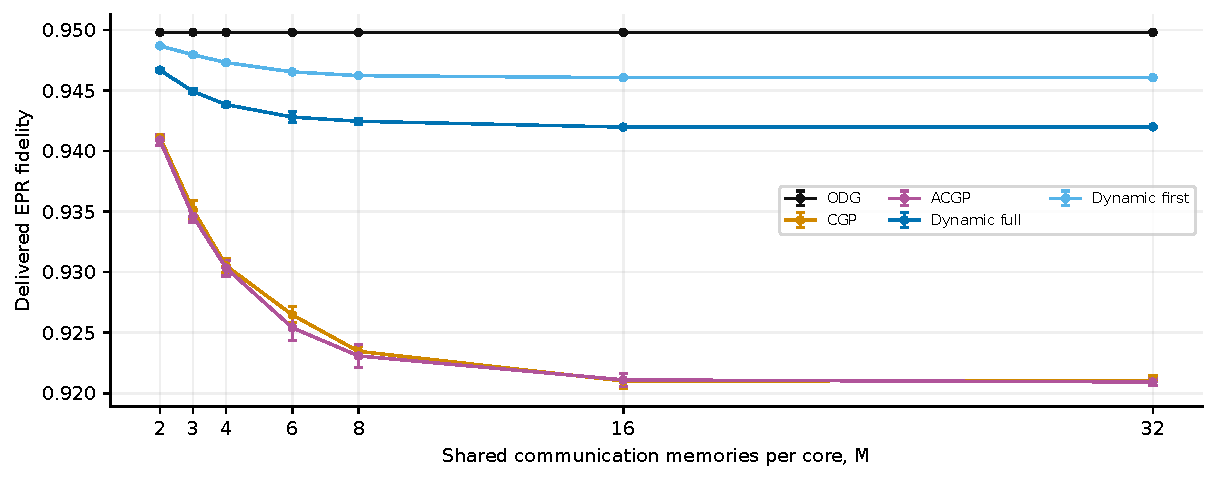
\includegraphics[width=.94\linewidth,height=.255\textheight,keepaspectratio]{figures/memory/mesh_shortest_reliable_average_delivered_epr_fidelity.pdf}\captionof{figure}{Run-level mean and sample SD. Shared trace aliases are counted once.}\end{center}
\begin{center}{\scriptsize\setlength{\tabcolsep}{3pt}
\begin{tabular}{lrrrrr}
\toprule
M & ODG & CGP & ACGP & Dynamic full & Dynamic first \\
\midrule
2 & $0.9498\pm0.0000$ & $0.9411\pm0.0002$ & $0.9409\pm0.0005$ & $0.9467\pm0.0001$ & $0.9487\pm0.0000$ \\
3 & $0.9498\pm0.0000$ & $0.9351\pm0.0008$ & $0.9346\pm0.0005$ & $0.9449\pm0.0002$ & $0.9480\pm0.0001$ \\
4 & $0.9498\pm0.0000$ & $0.9305\pm0.0006$ & $0.9303\pm0.0007$ & $0.9438\pm0.0001$ & $0.9473\pm0.0001$ \\
6 & $0.9498\pm0.0000$ & $0.9265\pm0.0007$ & $0.9254\pm0.0010$ & $0.9428\pm0.0004$ & $0.9465\pm0.0000$ \\
8 & $0.9498\pm0.0000$ & $0.9235\pm0.0004$ & $0.9231\pm0.0010$ & $0.9425\pm0.0002$ & $0.9462\pm0.0000$ \\
16 & $0.9498\pm0.0000$ & $0.9210\pm0.0006$ & $0.9211\pm0.0006$ & $0.9420\pm0.0000$ & $0.9461\pm0.0000$ \\
32 & $0.9498\pm0.0000$ & $0.9211\pm0.0004$ & $0.9209\pm0.0003$ & $0.9420\pm0.0000$ & $0.9461\pm0.0000$ \\
\bottomrule\end{tabular}}
\captionof{table}{Mean $\pm$ sample SD; n/a denotes a metric outside that policy's instrumentation.}
{\footnotesize\href{https://github.com/sanjeevkrishnaa/Compiler-Driven-ACE/blob/codex/ace-scheduler-correctness/docs/latex/qft96_final/data/memory_mesh_shortest_reliable_average_delivered_epr_fidelity.csv}{Exact CSV values and sample counts}}
\end{center}
\subsection*{Compiler readiness fraction}
\begin{center}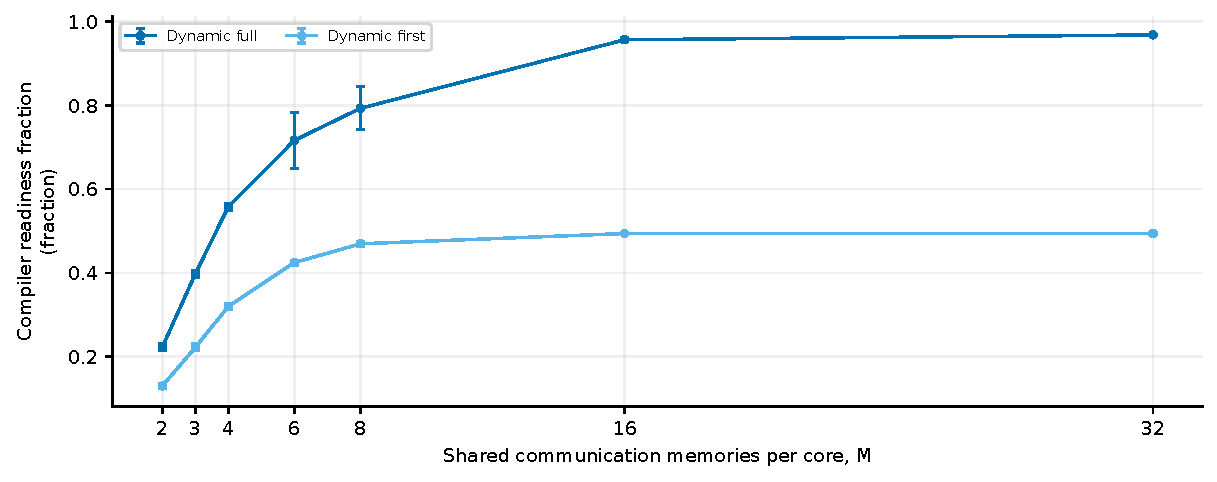
\includegraphics[width=.94\linewidth,height=.255\textheight,keepaspectratio]{figures/memory/mesh_shortest_reliable_pregenerated_success_rate.pdf}\captionof{figure}{Run-level mean and sample SD. Shared trace aliases are counted once.}\end{center}
\begin{center}{\scriptsize\setlength{\tabcolsep}{3pt}
\begin{tabular}{lrrrrr}
\toprule
M & ODG & CGP & ACGP & Dynamic full & Dynamic first \\
\midrule
2 & n/a & n/a & n/a & $0.2226\pm0.0087$ & $0.1299\pm0.0067$ \\
3 & n/a & n/a & n/a & $0.3976\pm0.0084$ & $0.2221\pm0.0083$ \\
4 & n/a & n/a & n/a & $0.5577\pm0.0084$ & $0.3197\pm0.0063$ \\
6 & n/a & n/a & n/a & $0.7165\pm0.0674$ & $0.4246\pm0.0058$ \\
8 & n/a & n/a & n/a & $0.7930\pm0.0516$ & $0.4695\pm0.0060$ \\
16 & n/a & n/a & n/a & $0.9567\pm0.0049$ & $0.4940\pm0.0016$ \\
32 & n/a & n/a & n/a & $0.9683\pm0.0013$ & $0.4940\pm0.0016$ \\
\bottomrule\end{tabular}}
\captionof{table}{Mean $\pm$ sample SD; n/a denotes a metric outside that policy's instrumentation.}
{\footnotesize\href{https://github.com/sanjeevkrishnaa/Compiler-Driven-ACE/blob/codex/ace-scheduler-correctness/docs/latex/qft96_final/data/memory_mesh_shortest_reliable_pregenerated_success_rate.csv}{Exact CSV values and sample counts}}
\end{center}
\clearpage
\subsection*{Intended compiler-hit fraction}
\begin{center}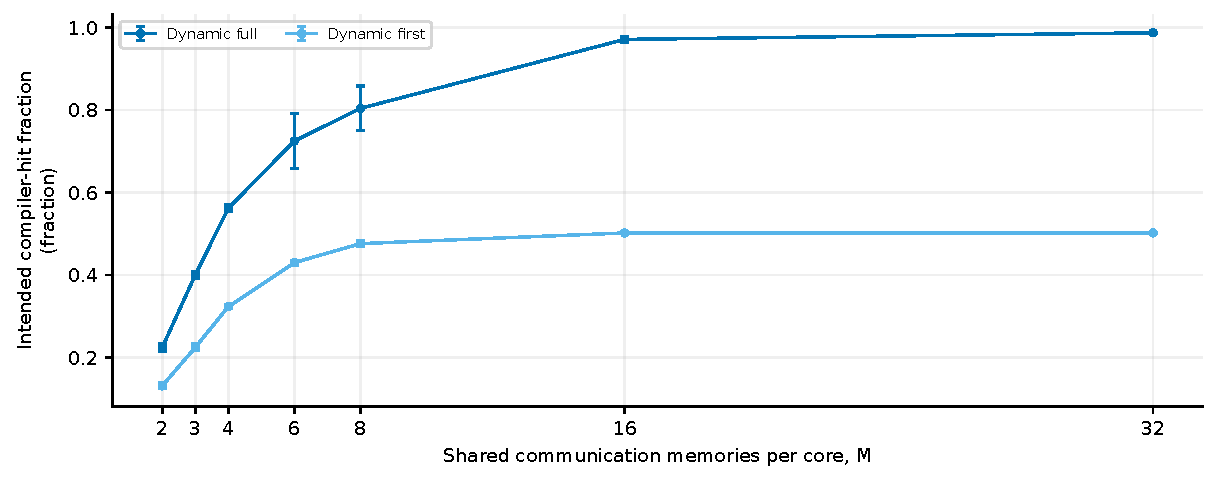
\includegraphics[width=.94\linewidth,height=.255\textheight,keepaspectratio]{figures/memory/mesh_shortest_reliable_intended_request_hit_rate.pdf}\captionof{figure}{Run-level mean and sample SD. Shared trace aliases are counted once.}\end{center}
\begin{center}{\scriptsize\setlength{\tabcolsep}{3pt}
\begin{tabular}{lrrrrr}
\toprule
M & ODG & CGP & ACGP & Dynamic full & Dynamic first \\
\midrule
2 & n/a & n/a & n/a & $0.2238\pm0.0089$ & $0.1309\pm0.0070$ \\
3 & n/a & n/a & n/a & $0.4000\pm0.0085$ & $0.2242\pm0.0085$ \\
4 & n/a & n/a & n/a & $0.5618\pm0.0079$ & $0.3231\pm0.0055$ \\
6 & n/a & n/a & n/a & $0.7248\pm0.0670$ & $0.4298\pm0.0063$ \\
8 & n/a & n/a & n/a & $0.8040\pm0.0543$ & $0.4759\pm0.0063$ \\
16 & n/a & n/a & n/a & $0.9713\pm0.0066$ & $0.5018\pm0.0015$ \\
32 & n/a & n/a & n/a & $0.9874\pm0.0011$ & $0.5018\pm0.0015$ \\
\bottomrule\end{tabular}}
\captionof{table}{Mean $\pm$ sample SD; n/a denotes a metric outside that policy's instrumentation.}
{\footnotesize\href{https://github.com/sanjeevkrishnaa/Compiler-Driven-ACE/blob/codex/ace-scheduler-correctness/docs/latex/qft96_final/data/memory_mesh_shortest_reliable_intended_request_hit_rate.csv}{Exact CSV values and sample counts}}
\end{center}
\subsection*{Compiler fallback fraction}
\begin{center}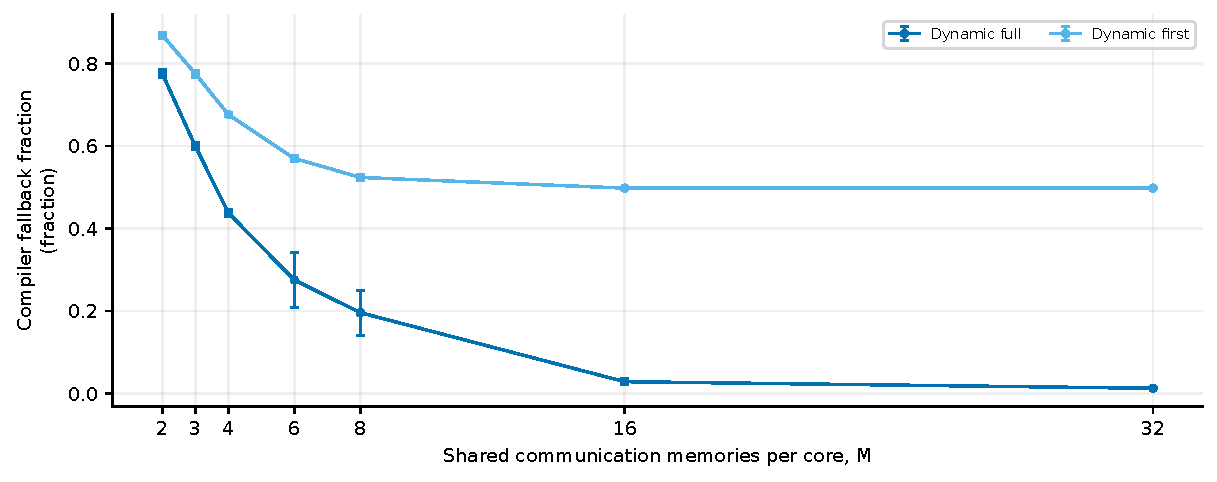
\includegraphics[width=.94\linewidth,height=.255\textheight,keepaspectratio]{figures/memory/mesh_shortest_reliable_on_demand_fallback_rate.pdf}\captionof{figure}{Run-level mean and sample SD. Shared trace aliases are counted once.}\end{center}
\begin{center}{\scriptsize\setlength{\tabcolsep}{3pt}
\begin{tabular}{lrrrrr}
\toprule
M & ODG & CGP & ACGP & Dynamic full & Dynamic first \\
\midrule
2 & n/a & n/a & n/a & $0.7762\pm0.0089$ & $0.8691\pm0.0070$ \\
3 & n/a & n/a & n/a & $0.6000\pm0.0085$ & $0.7758\pm0.0085$ \\
4 & n/a & n/a & n/a & $0.4382\pm0.0079$ & $0.6769\pm0.0055$ \\
6 & n/a & n/a & n/a & $0.2752\pm0.0670$ & $0.5702\pm0.0063$ \\
8 & n/a & n/a & n/a & $0.1960\pm0.0543$ & $0.5241\pm0.0063$ \\
16 & n/a & n/a & n/a & $0.0287\pm0.0066$ & $0.4982\pm0.0015$ \\
32 & n/a & n/a & n/a & $0.0126\pm0.0011$ & $0.4982\pm0.0015$ \\
\bottomrule\end{tabular}}
\captionof{table}{Mean $\pm$ sample SD; n/a denotes a metric outside that policy's instrumentation.}
{\footnotesize\href{https://github.com/sanjeevkrishnaa/Compiler-Driven-ACE/blob/codex/ace-scheduler-correctness/docs/latex/qft96_final/data/memory_mesh_shortest_reliable_on_demand_fallback_rate.csv}{Exact CSV values and sample counts}}
\end{center}
\clearpage
\subsection*{Compiler-cache waste}
\begin{center}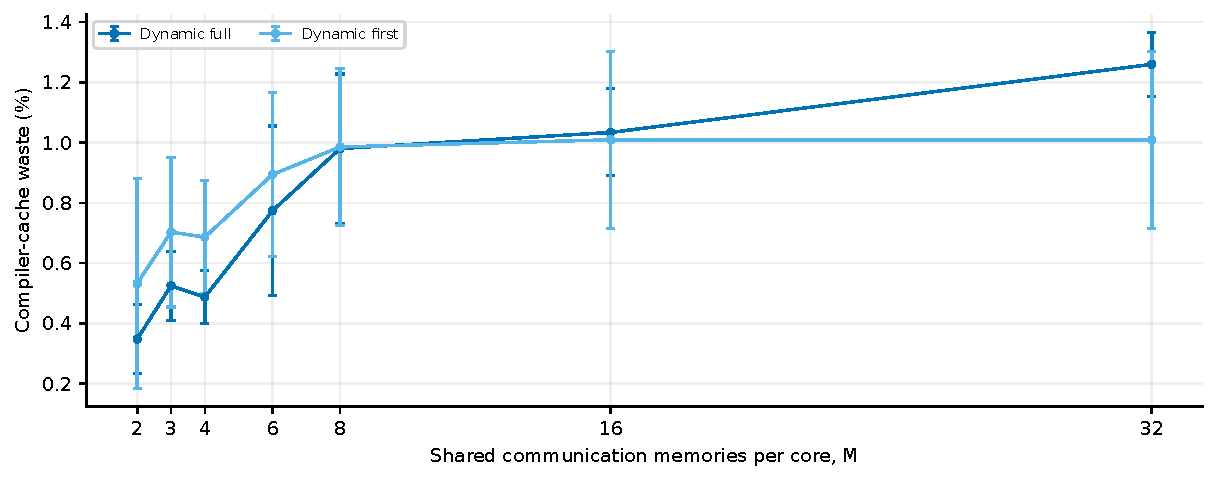
\includegraphics[width=.94\linewidth,height=.255\textheight,keepaspectratio]{figures/memory/mesh_shortest_reliable_compiler_waste_percentage.pdf}\captionof{figure}{Run-level mean and sample SD. Shared trace aliases are counted once.}\end{center}
\begin{center}{\scriptsize\setlength{\tabcolsep}{3pt}
\begin{tabular}{lrrrrr}
\toprule
M & ODG & CGP & ACGP & Dynamic full & Dynamic first \\
\midrule
2 & n/a & n/a & n/a & $0.3475\pm0.1140$ & $0.5320\pm0.3493$ \\
3 & n/a & n/a & n/a & $0.5248\pm0.1143$ & $0.7029\pm0.2488$ \\
4 & n/a & n/a & n/a & $0.4870\pm0.0873$ & $0.6862\pm0.1865$ \\
6 & n/a & n/a & n/a & $0.7735\pm0.2817$ & $0.8940\pm0.2733$ \\
8 & n/a & n/a & n/a & $0.9803\pm0.2475$ & $0.9856\pm0.2594$ \\
16 & n/a & n/a & n/a & $1.034\pm0.145$ & $1.009\pm0.294$ \\
32 & n/a & n/a & n/a & $1.260\pm0.106$ & $1.009\pm0.294$ \\
\bottomrule\end{tabular}}
\captionof{table}{Mean $\pm$ sample SD; n/a denotes a metric outside that policy's instrumentation.}
{\footnotesize\href{https://github.com/sanjeevkrishnaa/Compiler-Driven-ACE/blob/codex/ace-scheduler-correctness/docs/latex/qft96_final/data/memory_mesh_shortest_reliable_compiler_waste_percentage.csv}{Exact CSV values and sample counts}}
\end{center}
\subsection*{Native-protocol waste}
\begin{center}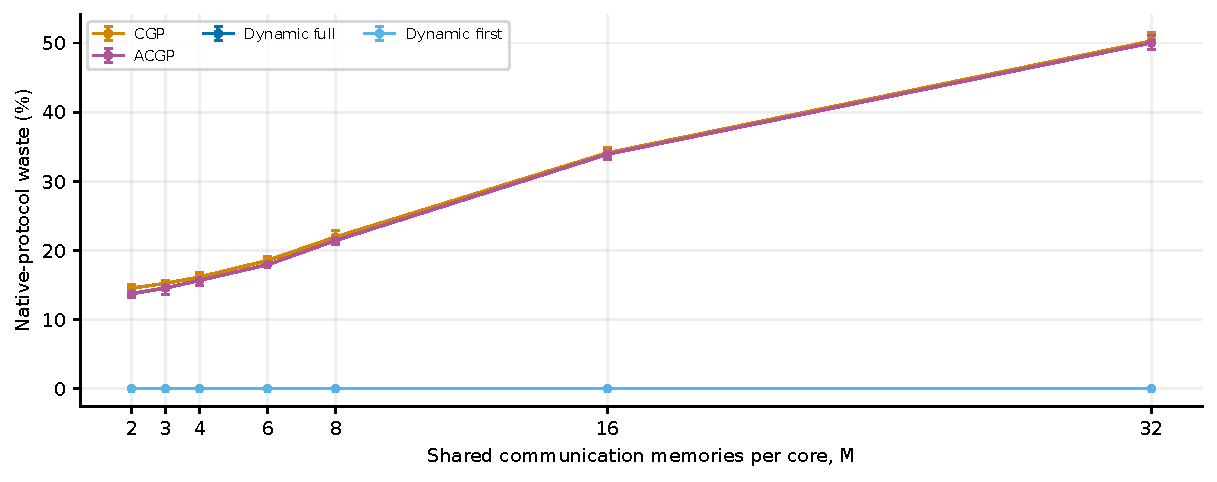
\includegraphics[width=.94\linewidth,height=.255\textheight,keepaspectratio]{figures/memory/mesh_shortest_reliable_protocol_waste_percentage.pdf}\captionof{figure}{Run-level mean and sample SD. Shared trace aliases are counted once.}\end{center}
\begin{center}{\scriptsize\setlength{\tabcolsep}{3pt}
\begin{tabular}{lrrrrr}
\toprule
M & ODG & CGP & ACGP & Dynamic full & Dynamic first \\
\midrule
2 & n/a & $14.553\pm0.495$ & $13.758\pm0.513$ & $0.0000\pm0.0000$ & $0.0000\pm0.0000$ \\
3 & n/a & $15.245\pm0.479$ & $14.578\pm0.972$ & $0.0000\pm0.0000$ & $0.0000\pm0.0000$ \\
4 & n/a & $16.160\pm0.590$ & $15.671\pm0.719$ & $0.0000\pm0.0000$ & $0.0000\pm0.0000$ \\
6 & n/a & $18.551\pm0.613$ & $17.943\pm0.129$ & $0.0000\pm0.0000$ & $0.0000\pm0.0000$ \\
8 & n/a & $21.953\pm0.935$ & $21.454\pm0.560$ & $0.0000\pm0.0000$ & $0.0000\pm0.0000$ \\
16 & n/a & $34.123\pm0.785$ & $33.927\pm0.719$ & $0.0000\pm0.0000$ & $0.0000\pm0.0000$ \\
32 & n/a & $50.300\pm1.267$ & $50.052\pm1.012$ & $0.0000\pm0.0000$ & $0.0000\pm0.0000$ \\
\bottomrule\end{tabular}}
\captionof{table}{Mean $\pm$ sample SD; n/a denotes a metric outside that policy's instrumentation.}
{\footnotesize\href{https://github.com/sanjeevkrishnaa/Compiler-Driven-ACE/blob/codex/ace-scheduler-correctness/docs/latex/qft96_final/data/memory_mesh_shortest_reliable_protocol_waste_percentage.csv}{Exact CSV values and sample counts}}
\end{center}
\clearpage
\subsection*{Compiler-pair expiry}
\begin{center}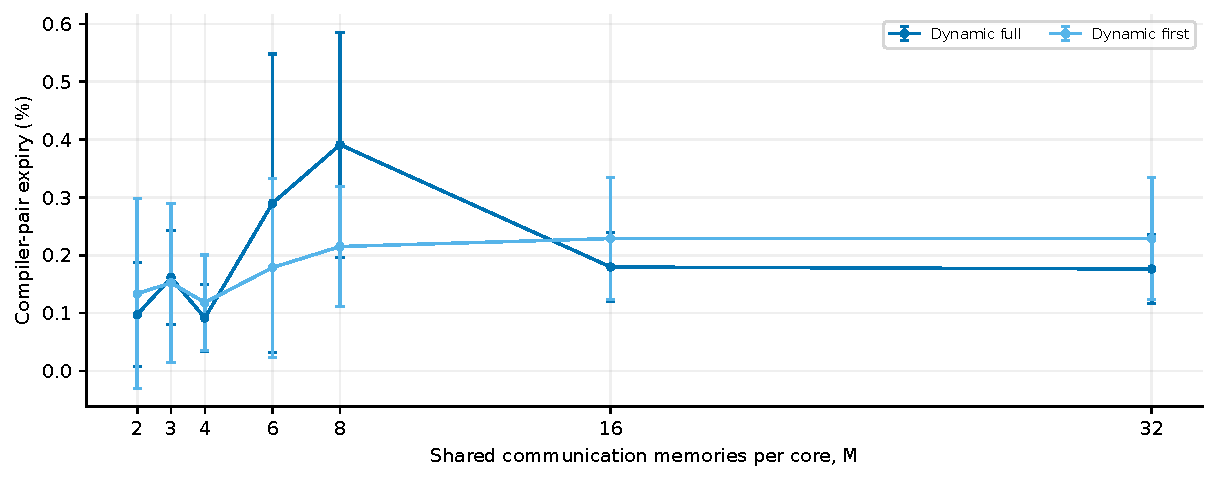
\includegraphics[width=.94\linewidth,height=.255\textheight,keepaspectratio]{figures/memory/mesh_shortest_reliable_compiler_expiry_percentage.pdf}\captionof{figure}{Run-level mean and sample SD. Shared trace aliases are counted once.}\end{center}
\begin{center}{\scriptsize\setlength{\tabcolsep}{3pt}
\begin{tabular}{lrrrrr}
\toprule
M & ODG & CGP & ACGP & Dynamic full & Dynamic first \\
\midrule
2 & n/a & n/a & n/a & $0.0973\pm0.0898$ & $0.1335\pm0.1642$ \\
3 & n/a & n/a & n/a & $0.1615\pm0.0810$ & $0.1526\pm0.1378$ \\
4 & n/a & n/a & n/a & $0.0916\pm0.0585$ & $0.1184\pm0.0822$ \\
6 & n/a & n/a & n/a & $0.2900\pm0.2580$ & $0.1788\pm0.1547$ \\
8 & n/a & n/a & n/a & $0.3913\pm0.1943$ & $0.2152\pm0.1031$ \\
16 & n/a & n/a & n/a & $0.1798\pm0.0591$ & $0.2290\pm0.1055$ \\
32 & n/a & n/a & n/a & $0.1763\pm0.0598$ & $0.2290\pm0.1055$ \\
\bottomrule\end{tabular}}
\captionof{table}{Mean $\pm$ sample SD; n/a denotes a metric outside that policy's instrumentation.}
{\footnotesize\href{https://github.com/sanjeevkrishnaa/Compiler-Driven-ACE/blob/codex/ace-scheduler-correctness/docs/latex/qft96_final/data/memory_mesh_shortest_reliable_compiler_expiry_percentage.csv}{Exact CSV values and sample counts}}
\end{center}
\subsection*{Used compiler-pair storage time}
\begin{center}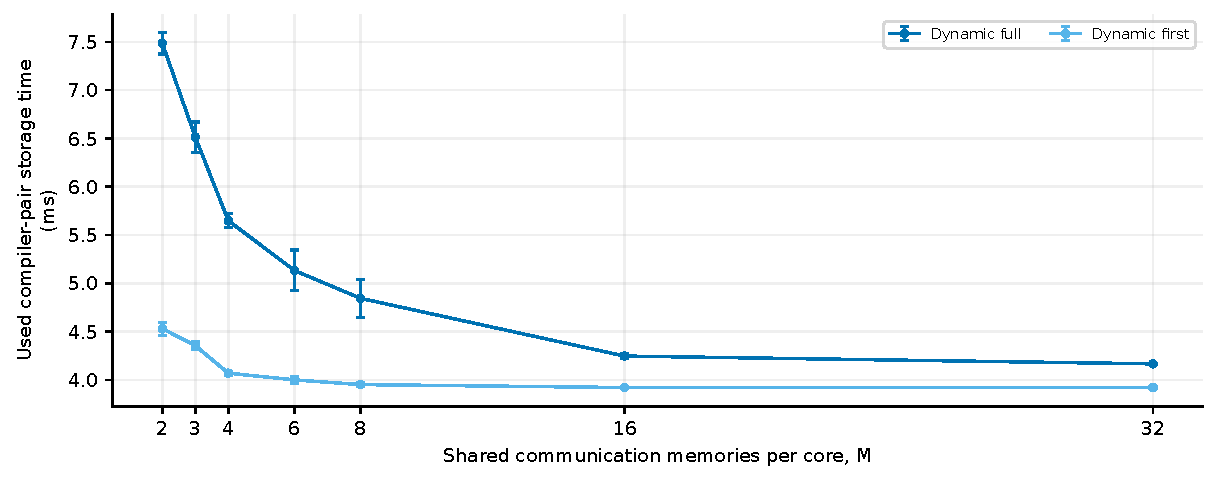
\includegraphics[width=.94\linewidth,height=.255\textheight,keepaspectratio]{figures/memory/mesh_shortest_reliable_average_storage_time_ms.pdf}\captionof{figure}{Run-level mean and sample SD. Shared trace aliases are counted once.}\end{center}
\begin{center}{\scriptsize\setlength{\tabcolsep}{3pt}
\begin{tabular}{lrrrrr}
\toprule
M & ODG & CGP & ACGP & Dynamic full & Dynamic first \\
\midrule
2 & n/a & n/a & n/a & $7.486\pm0.112$ & $4.531\pm0.068$ \\
3 & n/a & n/a & n/a & $6.514\pm0.156$ & $4.355\pm0.041$ \\
4 & n/a & n/a & n/a & $5.649\pm0.071$ & $4.070\pm0.019$ \\
6 & n/a & n/a & n/a & $5.133\pm0.211$ & $4.001\pm0.037$ \\
8 & n/a & n/a & n/a & $4.845\pm0.196$ & $3.952\pm0.019$ \\
16 & n/a & n/a & n/a & $4.247\pm0.027$ & $3.921\pm0.012$ \\
32 & n/a & n/a & n/a & $4.166\pm0.005$ & $3.921\pm0.012$ \\
\bottomrule\end{tabular}}
\captionof{table}{Mean $\pm$ sample SD; n/a denotes a metric outside that policy's instrumentation.}
{\footnotesize\href{https://github.com/sanjeevkrishnaa/Compiler-Driven-ACE/blob/codex/ace-scheduler-correctness/docs/latex/qft96_final/data/memory_mesh_shortest_reliable_average_storage_time_ms.csv}{Exact CSV values and sample counts}}
\end{center}
\clearpage
\subsection*{Delivered-hop throughput}
\begin{center}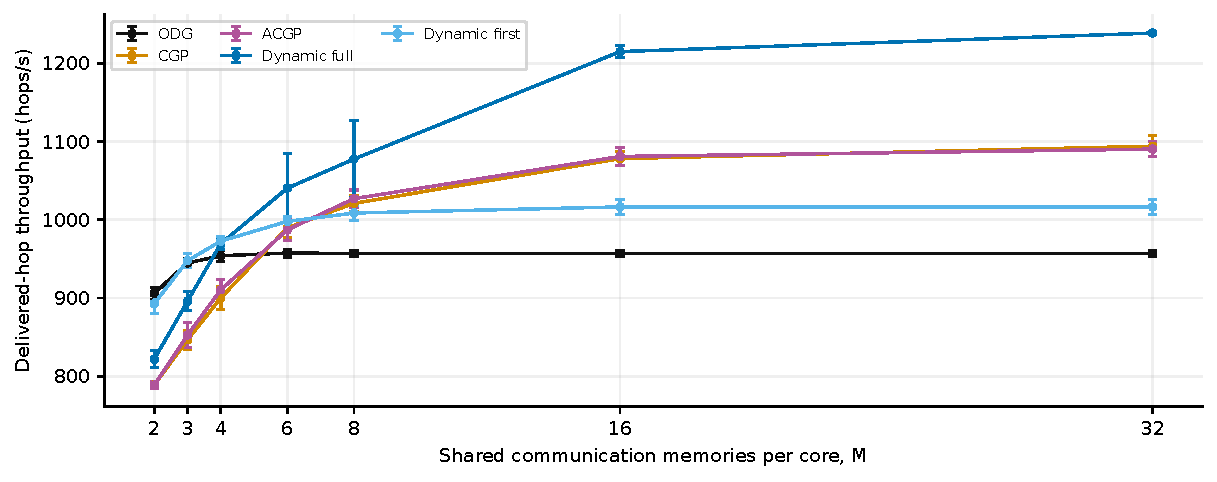
\includegraphics[width=.94\linewidth,height=.255\textheight,keepaspectratio]{figures/memory/mesh_shortest_reliable_hop_throughput_s.pdf}\captionof{figure}{Run-level mean and sample SD. Shared trace aliases are counted once.}\end{center}
\begin{center}{\scriptsize\setlength{\tabcolsep}{3pt}
\begin{tabular}{lrrrrr}
\toprule
M & ODG & CGP & ACGP & Dynamic full & Dynamic first \\
\midrule
2 & $905.76\pm8.15$ & $788.85\pm4.92$ & $788.75\pm3.98$ & $821.61\pm10.93$ & $892.79\pm13.16$ \\
3 & $944.69\pm5.99$ & $846.52\pm11.93$ & $852.55\pm15.77$ & $895.90\pm12.18$ & $947.66\pm8.99$ \\
4 & $953.88\pm6.91$ & $900.10\pm14.72$ & $910.38\pm12.82$ & $969.43\pm7.48$ & $972.64\pm6.28$ \\
6 & $957.40\pm5.06$ & $989.64\pm13.04$ & $987.06\pm13.48$ & $1040.35\pm44.31$ & $997.83\pm6.04$ \\
8 & $956.81\pm3.94$ & $1020.92\pm10.52$ & $1026.88\pm11.06$ & $1077.45\pm49.03$ & $1008.54\pm9.10$ \\
16 & $956.81\pm3.96$ & $1078.06\pm9.00$ & $1080.84\pm11.84$ & $1214.84\pm7.44$ & $1016.34\pm9.40$ \\
32 & $956.81\pm3.96$ & $1093.98\pm13.19$ & $1090.23\pm9.98$ & $1238.57\pm0.93$ & $1016.34\pm9.40$ \\
\bottomrule\end{tabular}}
\captionof{table}{Mean $\pm$ sample SD; n/a denotes a metric outside that policy's instrumentation.}
{\footnotesize\href{https://github.com/sanjeevkrishnaa/Compiler-Driven-ACE/blob/codex/ace-scheduler-correctness/docs/latex/qft96_final/data/memory_mesh_shortest_reliable_hop_throughput_s.csv}{Exact CSV values and sample counts}}
\end{center}
\subsection*{Completion fraction}
\begin{center}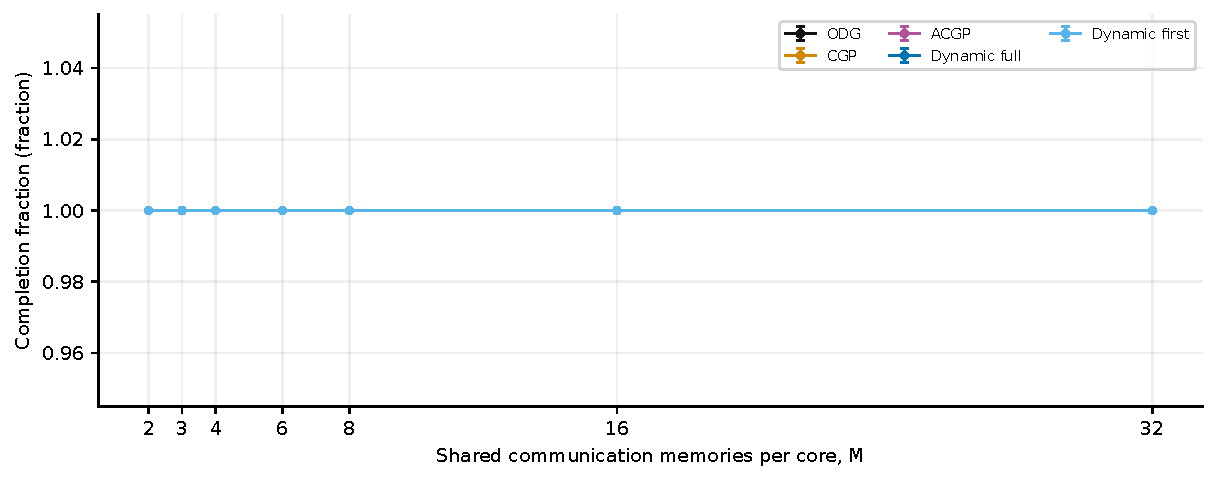
\includegraphics[width=.94\linewidth,height=.255\textheight,keepaspectratio]{figures/memory/mesh_shortest_reliable_completion_rate.pdf}\captionof{figure}{Run-level mean and sample SD. Shared trace aliases are counted once.}\end{center}
\begin{center}{\scriptsize\setlength{\tabcolsep}{3pt}
\begin{tabular}{lrrrrr}
\toprule
M & ODG & CGP & ACGP & Dynamic full & Dynamic first \\
\midrule
2 & $1.000\pm0.000$ & $1.000\pm0.000$ & $1.000\pm0.000$ & $1.000\pm0.000$ & $1.000\pm0.000$ \\
3 & $1.000\pm0.000$ & $1.000\pm0.000$ & $1.000\pm0.000$ & $1.000\pm0.000$ & $1.000\pm0.000$ \\
4 & $1.000\pm0.000$ & $1.000\pm0.000$ & $1.000\pm0.000$ & $1.000\pm0.000$ & $1.000\pm0.000$ \\
6 & $1.000\pm0.000$ & $1.000\pm0.000$ & $1.000\pm0.000$ & $1.000\pm0.000$ & $1.000\pm0.000$ \\
8 & $1.000\pm0.000$ & $1.000\pm0.000$ & $1.000\pm0.000$ & $1.000\pm0.000$ & $1.000\pm0.000$ \\
16 & $1.000\pm0.000$ & $1.000\pm0.000$ & $1.000\pm0.000$ & $1.000\pm0.000$ & $1.000\pm0.000$ \\
32 & $1.000\pm0.000$ & $1.000\pm0.000$ & $1.000\pm0.000$ & $1.000\pm0.000$ & $1.000\pm0.000$ \\
\bottomrule\end{tabular}}
\captionof{table}{Mean $\pm$ sample SD; n/a denotes a metric outside that policy's instrumentation.}
{\footnotesize\href{https://github.com/sanjeevkrishnaa/Compiler-Driven-ACE/blob/codex/ace-scheduler-correctness/docs/latex/qft96_final/data/memory_mesh_shortest_reliable_completion_rate.csv}{Exact CSV values and sample counts}}
\end{center}
\clearpage
\subsection*{Maximum admission wait}
\begin{center}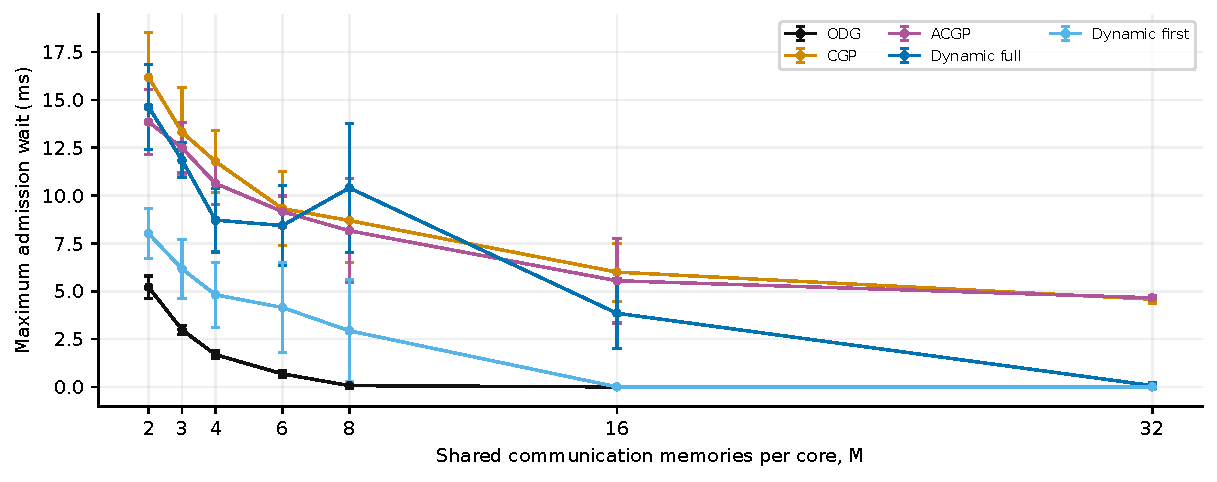
\includegraphics[width=.94\linewidth,height=.255\textheight,keepaspectratio]{figures/memory/mesh_shortest_reliable_max_admission_wait_ms.pdf}\captionof{figure}{Run-level mean and sample SD. Shared trace aliases are counted once.}\end{center}
\begin{center}{\scriptsize\setlength{\tabcolsep}{3pt}
\begin{tabular}{lrrrrr}
\toprule
M & ODG & CGP & ACGP & Dynamic full & Dynamic first \\
\midrule
2 & $5.217\pm0.581$ & $16.183\pm2.352$ & $13.850\pm1.714$ & $14.634\pm2.210$ & $8.017\pm1.286$ \\
3 & $2.983\pm0.248$ & $13.317\pm2.337$ & $12.494\pm1.313$ & $11.850\pm0.916$ & $6.167\pm1.546$ \\
4 & $1.683\pm0.194$ & $11.784\pm1.614$ & $10.634\pm1.117$ & $8.717\pm1.664$ & $4.817\pm1.708$ \\
6 & $0.6834\pm0.1941$ & $9.317\pm1.920$ & $9.167\pm0.812$ & $8.434\pm2.085$ & $4.150\pm2.374$ \\
8 & $0.0667\pm0.1633$ & $8.697\pm2.182$ & $8.163\pm2.716$ & $10.400\pm3.368$ & $2.933\pm2.666$ \\
16 & $0.0000\pm0.0000$ & $6.000\pm1.513$ & $5.550\pm2.210$ & $3.850\pm1.838$ & $0.0000\pm0.0000$ \\
32 & $0.0000\pm0.0000$ & $4.583\pm0.214$ & $4.657\pm0.136$ & $0.0667\pm0.1633$ & $0.0000\pm0.0000$ \\
\bottomrule\end{tabular}}
\captionof{table}{Mean $\pm$ sample SD; n/a denotes a metric outside that policy's instrumentation.}
{\footnotesize\href{https://github.com/sanjeevkrishnaa/Compiler-Driven-ACE/blob/codex/ace-scheduler-correctness/docs/latex/qft96_final/data/memory_mesh_shortest_reliable_max_admission_wait_ms.csv}{Exact CSV values and sample counts}}
\end{center}
\subsection*{Requests with admission wait}
\begin{center}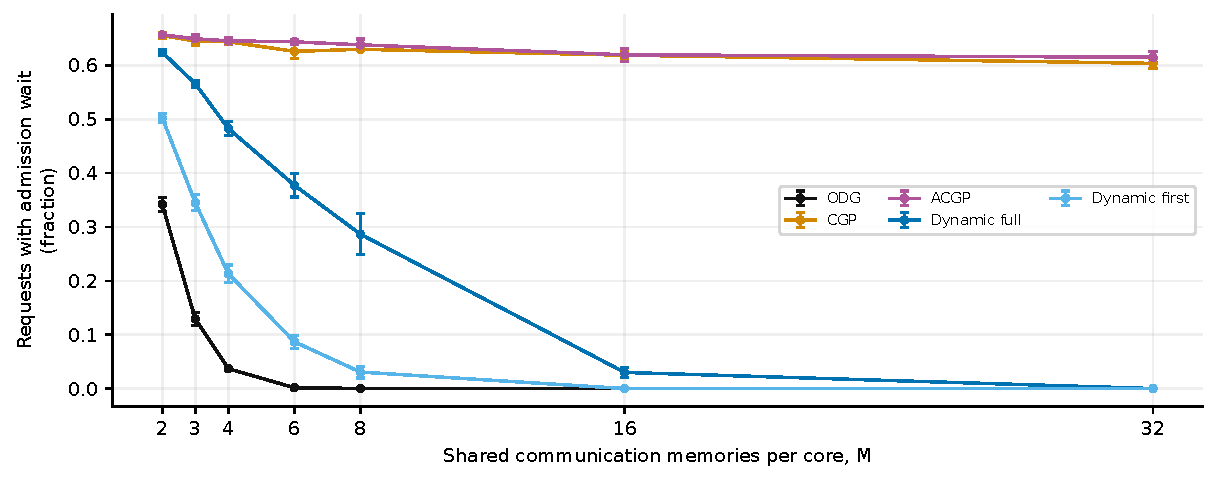
\includegraphics[width=.94\linewidth,height=.255\textheight,keepaspectratio]{figures/memory/mesh_shortest_reliable_requests_that_waited_fraction.pdf}\captionof{figure}{Run-level mean and sample SD. Shared trace aliases are counted once.}\end{center}
\begin{center}{\scriptsize\setlength{\tabcolsep}{3pt}
\begin{tabular}{lrrrrr}
\toprule
M & ODG & CGP & ACGP & Dynamic full & Dynamic first \\
\midrule
2 & $0.3419\pm0.0136$ & $0.6555\pm0.0058$ & $0.6567\pm0.0030$ & $0.6242\pm0.0053$ & $0.5027\pm0.0083$ \\
3 & $0.1292\pm0.0118$ & $0.6452\pm0.0077$ & $0.6494\pm0.0074$ & $0.5659\pm0.0065$ & $0.3449\pm0.0149$ \\
4 & $0.0369\pm0.0026$ & $0.6439\pm0.0058$ & $0.6455\pm0.0068$ & $0.4828\pm0.0126$ & $0.2133\pm0.0162$ \\
6 & $0.0016\pm0.0013$ & $0.6260\pm0.0128$ & $0.6437\pm0.0048$ & $0.3775\pm0.0218$ & $0.0869\pm0.0123$ \\
8 & $0.0002\pm0.0005$ & $0.6299\pm0.0024$ & $0.6381\pm0.0108$ & $0.2866\pm0.0384$ & $0.0307\pm0.0110$ \\
16 & $0.0000\pm0.0000$ & $0.6189\pm0.0065$ & $0.6196\pm0.0123$ & $0.0300\pm0.0090$ & $0.0000\pm0.0000$ \\
32 & $0.0000\pm0.0000$ & $0.6037\pm0.0091$ & $0.6151\pm0.0101$ & $0.0000\pm0.0001$ & $0.0000\pm0.0000$ \\
\bottomrule\end{tabular}}
\captionof{table}{Mean $\pm$ sample SD; n/a denotes a metric outside that policy's instrumentation.}
{\footnotesize\href{https://github.com/sanjeevkrishnaa/Compiler-Driven-ACE/blob/codex/ace-scheduler-correctness/docs/latex/qft96_final/data/memory_mesh_shortest_reliable_requests_that_waited_fraction.csv}{Exact CSV values and sample counts}}
\end{center}
\clearpage
\subsection*{Recorded reservation-setup counter}
\begin{center}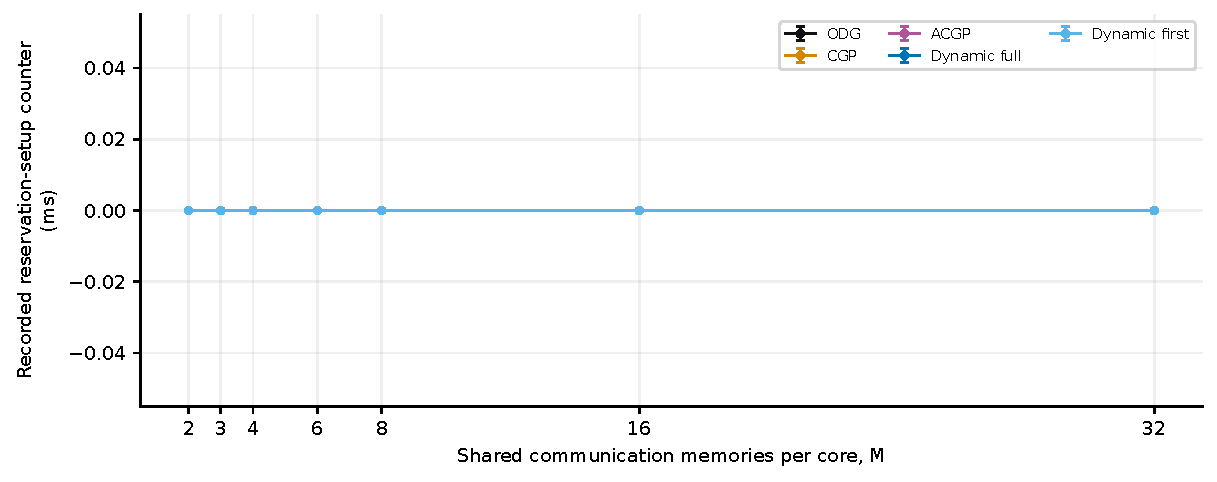
\includegraphics[width=.94\linewidth,height=.255\textheight,keepaspectratio]{figures/memory/mesh_shortest_reliable_avg_reservation_setup_time_ms.pdf}\captionof{figure}{Run-level mean and sample SD. Shared trace aliases are counted once.}\end{center}
\begin{center}{\scriptsize\setlength{\tabcolsep}{3pt}
\begin{tabular}{lrrrrr}
\toprule
M & ODG & CGP & ACGP & Dynamic full & Dynamic first \\
\midrule
2 & $0.0000\pm0.0000$ & $0.0000\pm0.0000$ & $0.0000\pm0.0000$ & $0.0000\pm0.0000$ & $0.0000\pm0.0000$ \\
3 & $0.0000\pm0.0000$ & $0.0000\pm0.0000$ & $0.0000\pm0.0000$ & $0.0000\pm0.0000$ & $0.0000\pm0.0000$ \\
4 & $0.0000\pm0.0000$ & $0.0000\pm0.0000$ & $0.0000\pm0.0000$ & $0.0000\pm0.0000$ & $0.0000\pm0.0000$ \\
6 & $0.0000\pm0.0000$ & $0.0000\pm0.0000$ & $0.0000\pm0.0000$ & $0.0000\pm0.0000$ & $0.0000\pm0.0000$ \\
8 & $0.0000\pm0.0000$ & $0.0000\pm0.0000$ & $0.0000\pm0.0000$ & $0.0000\pm0.0000$ & $0.0000\pm0.0000$ \\
16 & $0.0000\pm0.0000$ & $0.0000\pm0.0000$ & $0.0000\pm0.0000$ & $0.0000\pm0.0000$ & $0.0000\pm0.0000$ \\
32 & $0.0000\pm0.0000$ & $0.0000\pm0.0000$ & $0.0000\pm0.0000$ & $0.0000\pm0.0000$ & $0.0000\pm0.0000$ \\
\bottomrule\end{tabular}}
\captionof{table}{Mean $\pm$ sample SD; n/a denotes a metric outside that policy's instrumentation.}
{\footnotesize\href{https://github.com/sanjeevkrishnaa/Compiler-Driven-ACE/blob/codex/ace-scheduler-correctness/docs/latex/qft96_final/data/memory_mesh_shortest_reliable_avg_reservation_setup_time_ms.csv}{Exact CSV values and sample counts}}
\end{center}
\subsection*{Mean generation/service time}
\begin{center}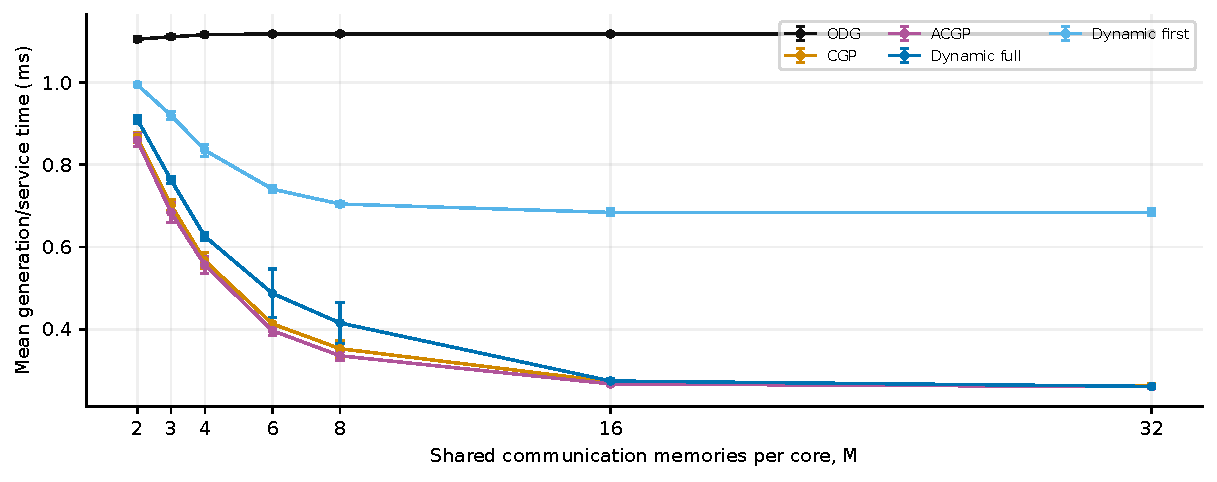
\includegraphics[width=.94\linewidth,height=.255\textheight,keepaspectratio]{figures/memory/mesh_shortest_reliable_avg_entanglement_generation_time_ms.pdf}\captionof{figure}{Run-level mean and sample SD. Shared trace aliases are counted once.}\end{center}
\begin{center}{\scriptsize\setlength{\tabcolsep}{3pt}
\begin{tabular}{lrrrrr}
\toprule
M & ODG & CGP & ACGP & Dynamic full & Dynamic first \\
\midrule
2 & $1.106\pm0.006$ & $0.8669\pm0.0124$ & $0.8600\pm0.0153$ & $0.9110\pm0.0092$ & $0.9952\pm0.0056$ \\
3 & $1.112\pm0.005$ & $0.7018\pm0.0143$ & $0.6844\pm0.0242$ & $0.7633\pm0.0080$ & $0.9207\pm0.0095$ \\
4 & $1.117\pm0.004$ & $0.5666\pm0.0197$ & $0.5561\pm0.0205$ & $0.6258\pm0.0107$ & $0.8356\pm0.0149$ \\
6 & $1.119\pm0.004$ & $0.4128\pm0.0148$ & $0.3965\pm0.0112$ & $0.4870\pm0.0595$ & $0.7408\pm0.0083$ \\
8 & $1.118\pm0.004$ & $0.3526\pm0.0210$ & $0.3352\pm0.0109$ & $0.4151\pm0.0497$ & $0.7046\pm0.0054$ \\
16 & $1.118\pm0.004$ & $0.2719\pm0.0053$ & $0.2668\pm0.0039$ & $0.2739\pm0.0061$ & $0.6841\pm0.0083$ \\
32 & $1.118\pm0.004$ & $0.2611\pm0.0061$ & $0.2599\pm0.0031$ & $0.2607\pm0.0011$ & $0.6841\pm0.0083$ \\
\bottomrule\end{tabular}}
\captionof{table}{Mean $\pm$ sample SD; n/a denotes a metric outside that policy's instrumentation.}
{\footnotesize\href{https://github.com/sanjeevkrishnaa/Compiler-Driven-ACE/blob/codex/ace-scheduler-correctness/docs/latex/qft96_final/data/memory_mesh_shortest_reliable_avg_entanglement_generation_time_ms.csv}{Exact CSV values and sample counts}}
\end{center}
\clearpage
\subsection*{Recorded retry-wait time}
\begin{center}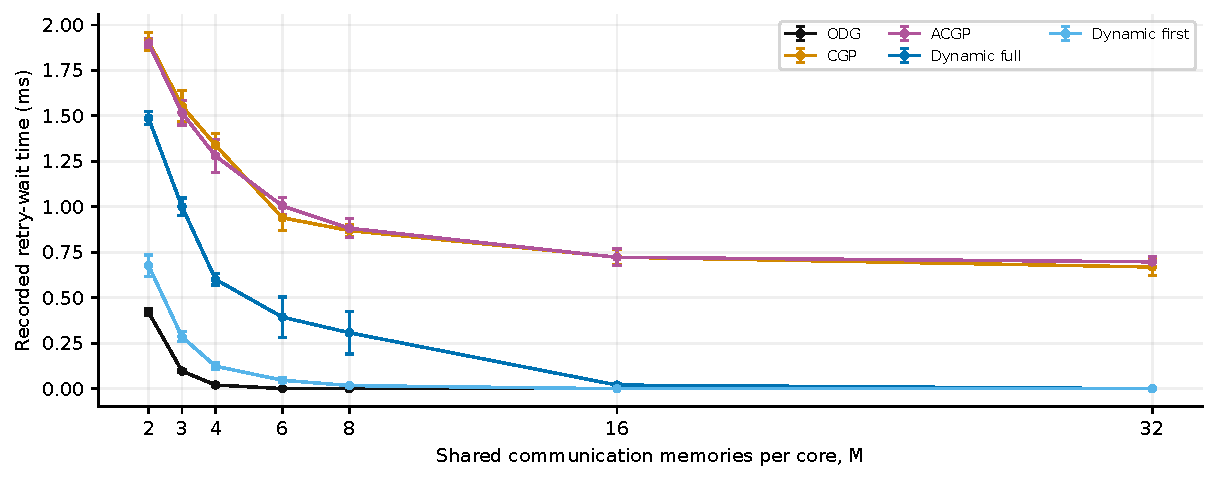
\includegraphics[width=.94\linewidth,height=.255\textheight,keepaspectratio]{figures/memory/mesh_shortest_reliable_avg_retry_wait_time_ms.pdf}\captionof{figure}{Run-level mean and sample SD. Shared trace aliases are counted once.}\end{center}
\begin{center}{\scriptsize\setlength{\tabcolsep}{3pt}
\begin{tabular}{lrrrrr}
\toprule
M & ODG & CGP & ACGP & Dynamic full & Dynamic first \\
\midrule
2 & $0.4199\pm0.0197$ & $1.909\pm0.050$ & $1.899\pm0.024$ & $1.487\pm0.035$ & $0.6768\pm0.0582$ \\
3 & $0.0969\pm0.0073$ & $1.553\pm0.084$ & $1.516\pm0.067$ & $0.9999\pm0.0484$ & $0.2848\pm0.0274$ \\
4 & $0.0205\pm0.0007$ & $1.339\pm0.063$ & $1.279\pm0.091$ & $0.6014\pm0.0313$ & $0.1240\pm0.0192$ \\
6 & $0.0007\pm0.0006$ & $0.9397\pm0.0707$ & $1.005\pm0.047$ & $0.3935\pm0.1107$ & $0.0467\pm0.0122$ \\
8 & $0.0000\pm0.0001$ & $0.8696\pm0.0338$ & $0.8822\pm0.0531$ & $0.3079\pm0.1170$ & $0.0174\pm0.0074$ \\
16 & $0.0000\pm0.0000$ & $0.7232\pm0.0409$ & $0.7222\pm0.0465$ & $0.0202\pm0.0073$ & $0.0000\pm0.0000$ \\
32 & $0.0000\pm0.0000$ & $0.6689\pm0.0479$ & $0.6974\pm0.0310$ & $0.0000\pm0.0000$ & $0.0000\pm0.0000$ \\
\bottomrule\end{tabular}}
\captionof{table}{Mean $\pm$ sample SD; n/a denotes a metric outside that policy's instrumentation.}
{\footnotesize\href{https://github.com/sanjeevkrishnaa/Compiler-Driven-ACE/blob/codex/ace-scheduler-correctness/docs/latex/qft96_final/data/memory_mesh_shortest_reliable_avg_retry_wait_time_ms.csv}{Exact CSV values and sample counts}}
\end{center}
\subsection*{Request retries}
\begin{center}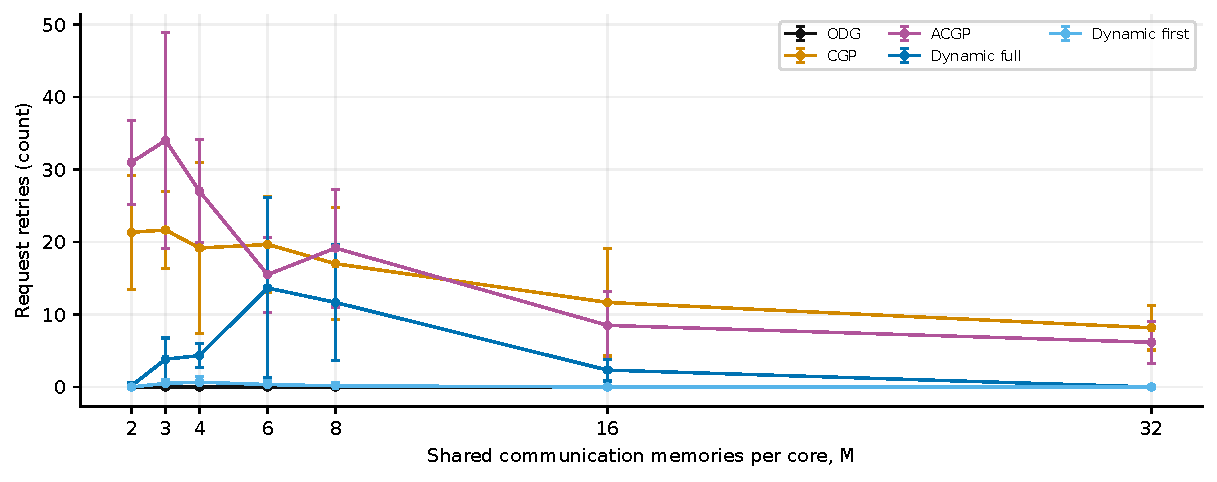
\includegraphics[width=.94\linewidth,height=.255\textheight,keepaspectratio]{figures/memory/mesh_shortest_reliable_total_retries.pdf}\captionof{figure}{Run-level mean and sample SD. Shared trace aliases are counted once.}\end{center}
\begin{center}{\scriptsize\setlength{\tabcolsep}{3pt}
\begin{tabular}{lrrrrr}
\toprule
M & ODG & CGP & ACGP & Dynamic full & Dynamic first \\
\midrule
2 & $0.0000\pm0.0000$ & $21.333\pm7.891$ & $31.000\pm5.762$ & $0.1667\pm0.4082$ & $0.0000\pm0.0000$ \\
3 & $0.0000\pm0.0000$ & $21.667\pm5.354$ & $34.000\pm14.926$ & $3.833\pm2.927$ & $0.5000\pm0.5477$ \\
4 & $0.0000\pm0.0000$ & $19.167\pm11.822$ & $27.000\pm7.099$ & $4.333\pm1.633$ & $0.6667\pm0.8165$ \\
6 & $0.0000\pm0.0000$ & $19.667\pm6.653$ & $15.500\pm5.167$ & $13.667\pm12.420$ & $0.3333\pm0.5164$ \\
8 & $0.0000\pm0.0000$ & $17.000\pm7.720$ & $19.167\pm8.134$ & $11.667\pm8.042$ & $0.1667\pm0.4082$ \\
16 & $0.0000\pm0.0000$ & $11.667\pm7.394$ & $8.500\pm4.722$ & $2.333\pm1.506$ & $0.0000\pm0.0000$ \\
32 & $0.0000\pm0.0000$ & $8.167\pm3.061$ & $6.167\pm2.927$ & $0.0000\pm0.0000$ & $0.0000\pm0.0000$ \\
\bottomrule\end{tabular}}
\captionof{table}{Mean $\pm$ sample SD; n/a denotes a metric outside that policy's instrumentation.}
{\footnotesize\href{https://github.com/sanjeevkrishnaa/Compiler-Driven-ACE/blob/codex/ace-scheduler-correctness/docs/latex/qft96_final/data/memory_mesh_shortest_reliable_total_retries.csv}{Exact CSV values and sample counts}}
\end{center}
\clearpage
\subsection*{Requests with retries}
\begin{center}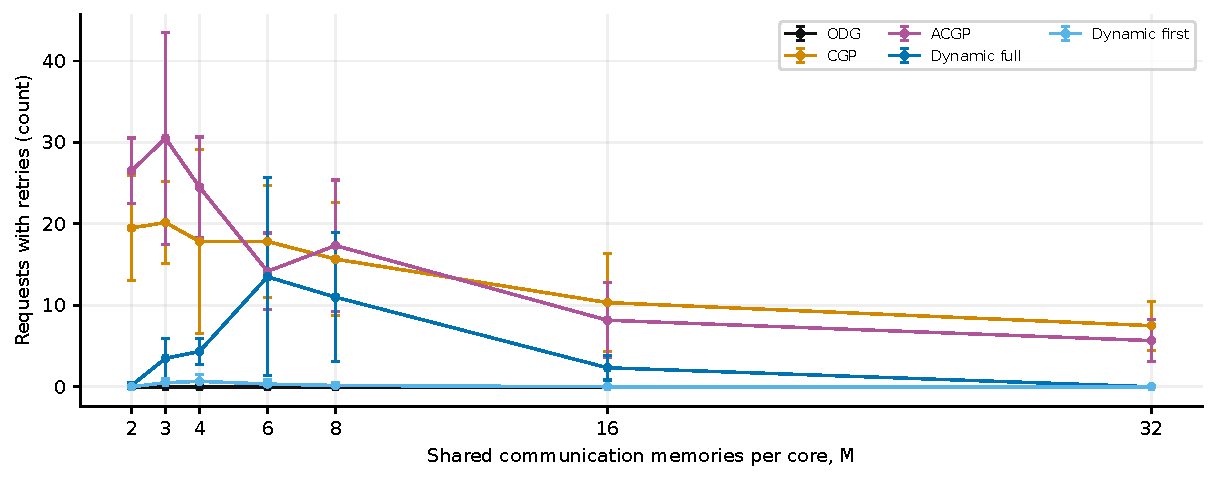
\includegraphics[width=.94\linewidth,height=.255\textheight,keepaspectratio]{figures/memory/mesh_shortest_reliable_requests_with_retries.pdf}\captionof{figure}{Run-level mean and sample SD. Shared trace aliases are counted once.}\end{center}
\begin{center}{\scriptsize\setlength{\tabcolsep}{3pt}
\begin{tabular}{lrrrrr}
\toprule
M & ODG & CGP & ACGP & Dynamic full & Dynamic first \\
\midrule
2 & $0.0000\pm0.0000$ & $19.500\pm6.442$ & $26.500\pm4.037$ & $0.1667\pm0.4082$ & $0.0000\pm0.0000$ \\
3 & $0.0000\pm0.0000$ & $20.167\pm5.037$ & $30.500\pm13.004$ & $3.500\pm2.429$ & $0.5000\pm0.5477$ \\
4 & $0.0000\pm0.0000$ & $17.833\pm11.286$ & $24.500\pm6.156$ & $4.333\pm1.633$ & $0.6667\pm0.8165$ \\
6 & $0.0000\pm0.0000$ & $17.833\pm6.824$ & $14.167\pm4.708$ & $13.500\pm12.161$ & $0.3333\pm0.5164$ \\
8 & $0.0000\pm0.0000$ & $15.667\pm6.919$ & $17.333\pm8.042$ & $11.000\pm7.899$ & $0.1667\pm0.4082$ \\
16 & $0.0000\pm0.0000$ & $10.333\pm6.055$ & $8.167\pm4.622$ & $2.333\pm1.506$ & $0.0000\pm0.0000$ \\
32 & $0.0000\pm0.0000$ & $7.500\pm3.017$ & $5.667\pm2.582$ & $0.0000\pm0.0000$ & $0.0000\pm0.0000$ \\
\bottomrule\end{tabular}}
\captionof{table}{Mean $\pm$ sample SD; n/a denotes a metric outside that policy's instrumentation.}
{\footnotesize\href{https://github.com/sanjeevkrishnaa/Compiler-Driven-ACE/blob/codex/ace-scheduler-correctness/docs/latex/qft96_final/data/memory_mesh_shortest_reliable_requests_with_retries.csv}{Exact CSV values and sample counts}}
\end{center}
\subsection*{Native-protocol generated-pair counter}
\begin{center}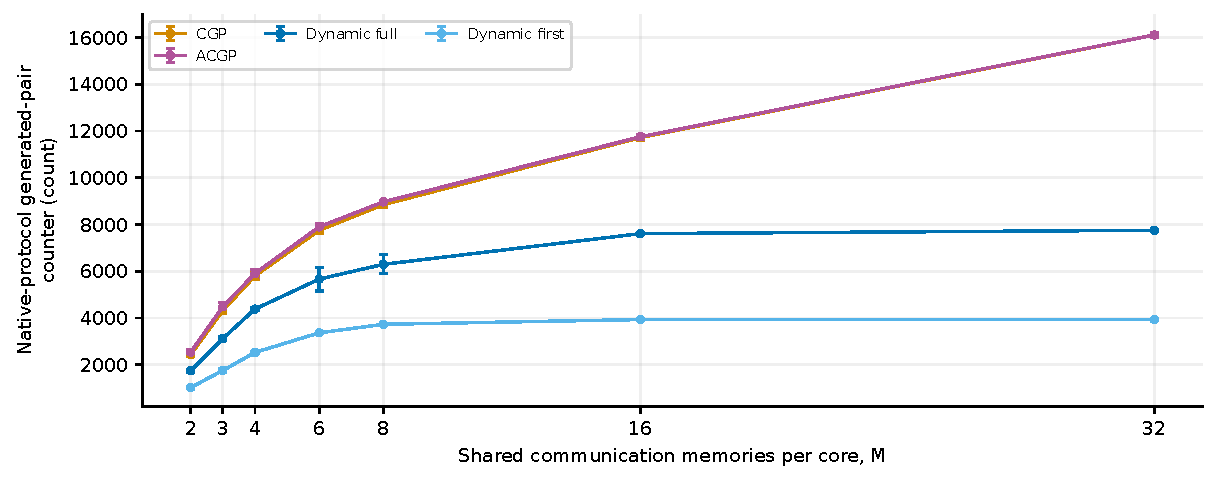
\includegraphics[width=.94\linewidth,height=.255\textheight,keepaspectratio]{figures/memory/mesh_shortest_reliable_protocol_generated_pairs.pdf}\captionof{figure}{Run-level mean and sample SD. Shared trace aliases are counted once.}\end{center}
\begin{center}{\scriptsize\setlength{\tabcolsep}{3pt}
\begin{tabular}{lrrrrr}
\toprule
M & ODG & CGP & ACGP & Dynamic full & Dynamic first \\
\midrule
2 & n/a & $2429.33\pm80.19$ & $2532.67\pm103.77$ & $1740.67\pm67.93$ & $1020.33\pm52.14$ \\
3 & n/a & $4318.67\pm125.64$ & $4478.00\pm189.63$ & $3117.00\pm64.99$ & $1750.00\pm67.54$ \\
4 & n/a & $5798.00\pm157.11$ & $5902.00\pm157.36$ & $4376.67\pm62.77$ & $2522.00\pm44.76$ \\
6 & n/a & $7752.33\pm121.27$ & $7898.00\pm122.64$ & $5661.00\pm508.95$ & $3362.00\pm43.12$ \\
8 & n/a & $8846.33\pm109.12$ & $8968.00\pm73.64$ & $6293.67\pm411.75$ & $3726.00\pm42.86$ \\
16 & n/a & $11719.33\pm114.94$ & $11751.67\pm112.46$ & $7608.00\pm53.56$ & $3930.00\pm0.00$ \\
32 & n/a & $16112.00\pm60.99$ & $16111.33\pm112.67$ & $7752.00\pm0.00$ & $3930.00\pm0.00$ \\
\bottomrule\end{tabular}}
\captionof{table}{Mean $\pm$ sample SD; n/a denotes a metric outside that policy's instrumentation.}
{\footnotesize\href{https://github.com/sanjeevkrishnaa/Compiler-Driven-ACE/blob/codex/ace-scheduler-correctness/docs/latex/qft96_final/data/memory_mesh_shortest_reliable_protocol_generated_pairs.csv}{Exact CSV values and sample counts}}
\end{center}
\clearpage
\subsection*{Native-protocol used-pair counter}
\begin{center}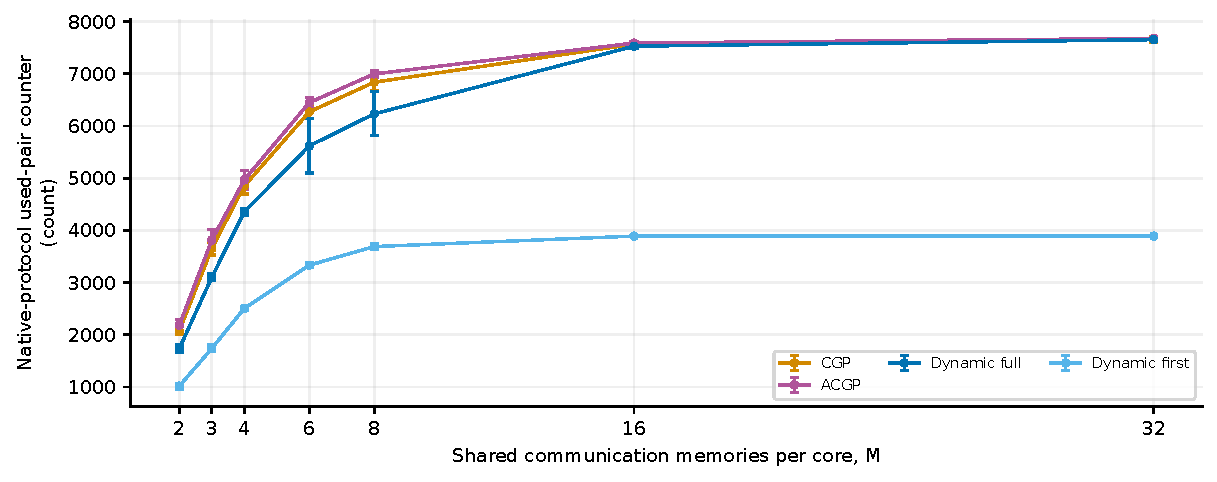
\includegraphics[width=.94\linewidth,height=.255\textheight,keepaspectratio]{figures/memory/mesh_shortest_reliable_protocol_used_pairs.pdf}\captionof{figure}{Run-level mean and sample SD. Shared trace aliases are counted once.}\end{center}
\begin{center}{\scriptsize\setlength{\tabcolsep}{3pt}
\begin{tabular}{lrrrrr}
\toprule
M & ODG & CGP & ACGP & Dynamic full & Dynamic first \\
\midrule
2 & n/a & $2073.33\pm76.59$ & $2182.67\pm102.42$ & $1734.67\pm69.21$ & $1015.00\pm54.31$ \\
3 & n/a & $3652.33\pm123.99$ & $3814.33\pm203.83$ & $3100.67\pm66.12$ & $1737.67\pm66.10$ \\
4 & n/a & $4850.00\pm152.65$ & $4967.33\pm175.54$ & $4355.33\pm61.11$ & $2504.67\pm42.89$ \\
6 & n/a & $6271.00\pm129.71$ & $6447.67\pm102.21$ & $5618.33\pm519.56$ & $3332.00\pm48.58$ \\
8 & n/a & $6839.00\pm158.87$ & $6998.00\pm60.37$ & $6232.67\pm420.75$ & $3689.33\pm49.08$ \\
16 & n/a & $7569.00\pm48.16$ & $7589.33\pm34.86$ & $7529.33\pm51.02$ & $3890.33\pm11.55$ \\
32 & n/a & $7656.33\pm51.22$ & $7678.67\pm22.44$ & $7654.33\pm8.24$ & $3890.33\pm11.55$ \\
\bottomrule\end{tabular}}
\captionof{table}{Mean $\pm$ sample SD; n/a denotes a metric outside that policy's instrumentation.}
{\footnotesize\href{https://github.com/sanjeevkrishnaa/Compiler-Driven-ACE/blob/codex/ace-scheduler-correctness/docs/latex/qft96_final/data/memory_mesh_shortest_reliable_protocol_used_pairs.csv}{Exact CSV values and sample counts}}
\end{center}
\subsection*{Native-protocol unused-pair counter}
\begin{center}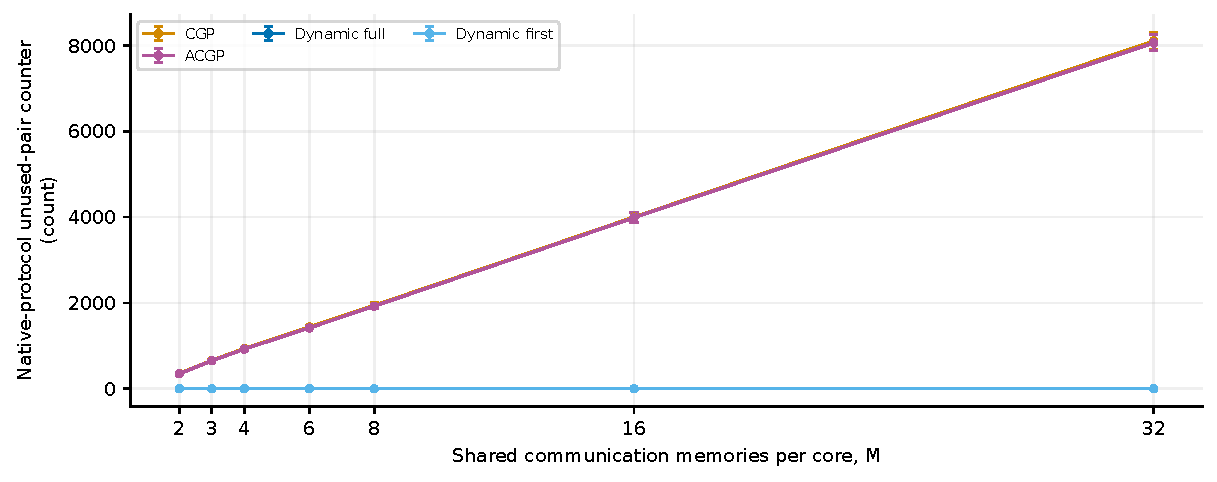
\includegraphics[width=.94\linewidth,height=.255\textheight,keepaspectratio]{figures/memory/mesh_shortest_reliable_protocol_unused_pairs.pdf}\captionof{figure}{Run-level mean and sample SD. Shared trace aliases are counted once.}\end{center}
\begin{center}{\scriptsize\setlength{\tabcolsep}{3pt}
\begin{tabular}{lrrrrr}
\toprule
M & ODG & CGP & ACGP & Dynamic full & Dynamic first \\
\midrule
2 & n/a & $353.33\pm10.41$ & $348.00\pm2.19$ & $0.0000\pm0.0000$ & $0.0000\pm0.0000$ \\
3 & n/a & $658.00\pm15.39$ & $651.33\pm16.86$ & $0.0000\pm0.0000$ & $0.0000\pm0.0000$ \\
4 & n/a & $936.33\pm21.96$ & $924.00\pm21.39$ & $0.0000\pm0.0000$ & $0.0000\pm0.0000$ \\
6 & n/a & $1437.67\pm33.88$ & $1417.00\pm12.88$ & $0.0000\pm0.0000$ & $0.0000\pm0.0000$ \\
8 & n/a & $1941.33\pm62.64$ & $1924.00\pm51.07$ & $0.0000\pm0.0000$ & $0.0000\pm0.0000$ \\
16 & n/a & $3999.33\pm114.57$ & $3987.67\pm120.58$ & $0.0000\pm0.0000$ & $0.0000\pm0.0000$ \\
32 & n/a & $8104.33\pm202.89$ & $8064.33\pm190.79$ & $0.0000\pm0.0000$ & $0.0000\pm0.0000$ \\
\bottomrule\end{tabular}}
\captionof{table}{Mean $\pm$ sample SD; n/a denotes a metric outside that policy's instrumentation.}
{\footnotesize\href{https://github.com/sanjeevkrishnaa/Compiler-Driven-ACE/blob/codex/ace-scheduler-correctness/docs/latex/qft96_final/data/memory_mesh_shortest_reliable_protocol_unused_pairs.csv}{Exact CSV values and sample counts}}
\end{center}
\clearpage
\subsection*{Scheduled compiler preparations}
\begin{center}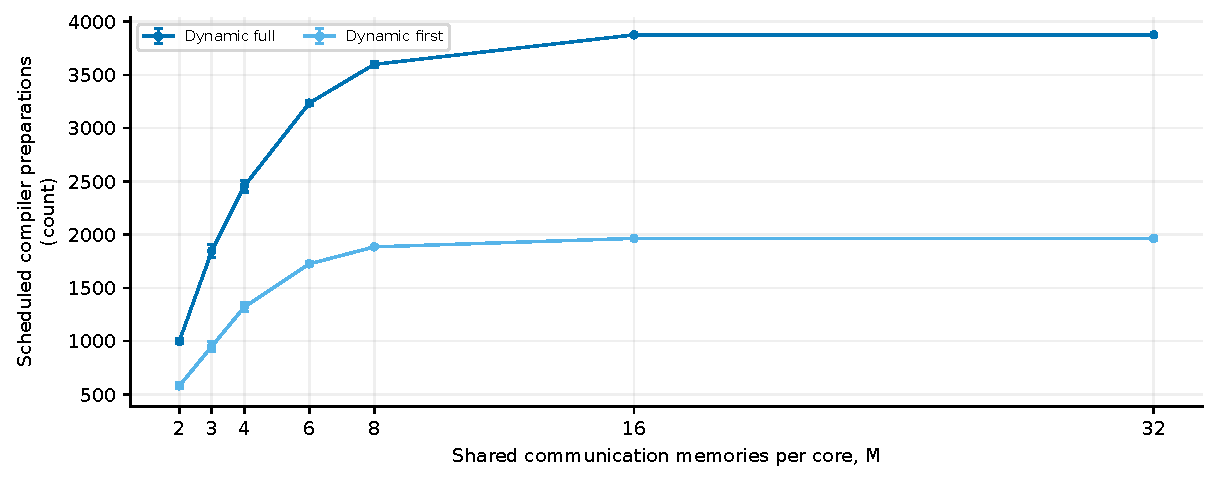
\includegraphics[width=.94\linewidth,height=.255\textheight,keepaspectratio]{figures/memory/mesh_shortest_reliable_scheduled_preparations.pdf}\captionof{figure}{Run-level mean and sample SD. Shared trace aliases are counted once.}\end{center}
\begin{center}{\scriptsize\setlength{\tabcolsep}{3pt}
\begin{tabular}{lrrrrr}
\toprule
M & ODG & CGP & ACGP & Dynamic full & Dynamic first \\
\midrule
2 & n/a & n/a & n/a & $999.00\pm24.93$ & $580.00\pm27.90$ \\
3 & n/a & n/a & n/a & $1846.33\pm57.91$ & $951.00\pm50.11$ \\
4 & n/a & n/a & n/a & $2455.67\pm55.36$ & $1320.33\pm38.55$ \\
6 & n/a & n/a & n/a & $3235.00\pm24.93$ & $1725.33\pm17.76$ \\
8 & n/a & n/a & n/a & $3598.67\pm30.27$ & $1885.00\pm8.81$ \\
16 & n/a & n/a & n/a & $3875.67\pm0.52$ & $1965.00\pm0.00$ \\
32 & n/a & n/a & n/a & $3876.00\pm0.00$ & $1965.00\pm0.00$ \\
\bottomrule\end{tabular}}
\captionof{table}{Mean $\pm$ sample SD; n/a denotes a metric outside that policy's instrumentation.}
{\footnotesize\href{https://github.com/sanjeevkrishnaa/Compiler-Driven-ACE/blob/codex/ace-scheduler-correctness/docs/latex/qft96_final/data/memory_mesh_shortest_reliable_scheduled_preparations.csv}{Exact CSV values and sample counts}}
\end{center}
\subsection*{Planner-blocked preparations}
\begin{center}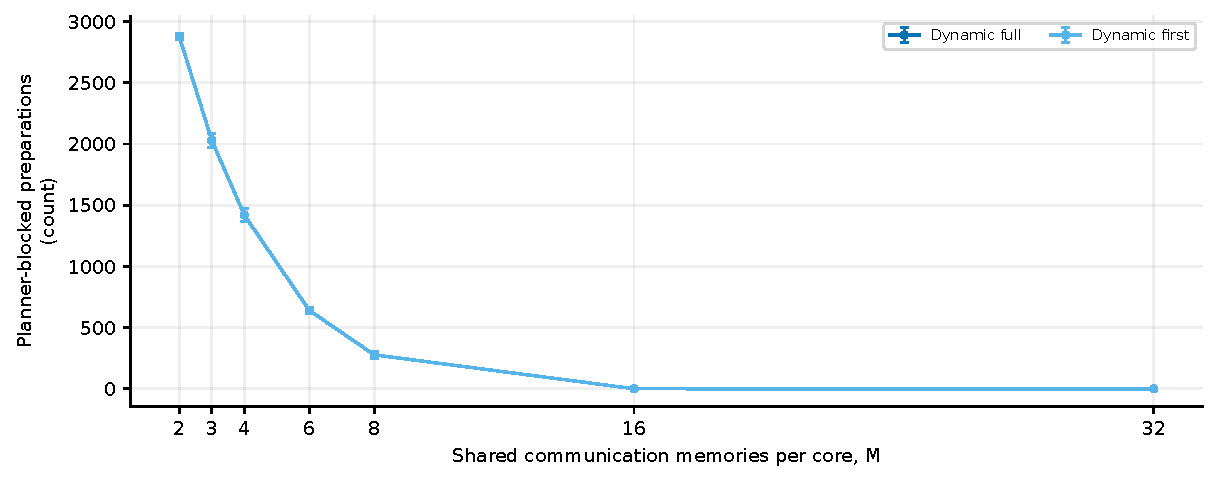
\includegraphics[width=.94\linewidth,height=.255\textheight,keepaspectratio]{figures/memory/mesh_shortest_reliable_planner_blocked_preparations.pdf}\captionof{figure}{Run-level mean and sample SD. Shared trace aliases are counted once.}\end{center}
\begin{center}{\scriptsize\setlength{\tabcolsep}{3pt}
\begin{tabular}{lrrrrr}
\toprule
M & ODG & CGP & ACGP & Dynamic full & Dynamic first \\
\midrule
2 & n/a & n/a & n/a & $2877.00\pm24.93$ & $2877.00\pm24.93$ \\
3 & n/a & n/a & n/a & $2029.67\pm57.91$ & $2029.67\pm57.91$ \\
4 & n/a & n/a & n/a & $1420.33\pm55.36$ & $1420.33\pm55.36$ \\
6 & n/a & n/a & n/a & $641.00\pm24.93$ & $641.00\pm24.93$ \\
8 & n/a & n/a & n/a & $277.33\pm30.27$ & $277.33\pm30.27$ \\
16 & n/a & n/a & n/a & $0.3333\pm0.5164$ & $0.3333\pm0.5164$ \\
32 & n/a & n/a & n/a & $0.0000\pm0.0000$ & $0.0000\pm0.0000$ \\
\bottomrule\end{tabular}}
\captionof{table}{Mean $\pm$ sample SD; n/a denotes a metric outside that policy's instrumentation.}
{\footnotesize\href{https://github.com/sanjeevkrishnaa/Compiler-Driven-ACE/blob/codex/ace-scheduler-correctness/docs/latex/qft96_final/data/memory_mesh_shortest_reliable_planner_blocked_preparations.csv}{Exact CSV values and sample counts}}
\end{center}
\clearpage
\subsection*{Planner peak compiler memory}
\begin{center}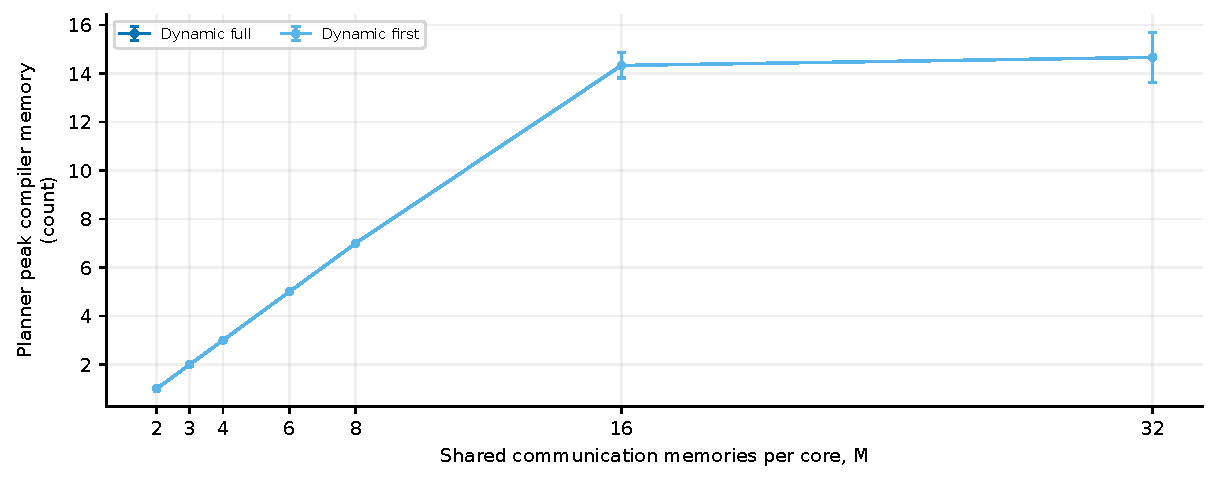
\includegraphics[width=.94\linewidth,height=.255\textheight,keepaspectratio]{figures/memory/mesh_shortest_reliable_planner_peak_compiler_memory_per_core.pdf}\captionof{figure}{Run-level mean and sample SD. Shared trace aliases are counted once.}\end{center}
\begin{center}{\scriptsize\setlength{\tabcolsep}{3pt}
\begin{tabular}{lrrrrr}
\toprule
M & ODG & CGP & ACGP & Dynamic full & Dynamic first \\
\midrule
2 & n/a & n/a & n/a & $1.000\pm0.000$ & $1.000\pm0.000$ \\
3 & n/a & n/a & n/a & $2.000\pm0.000$ & $2.000\pm0.000$ \\
4 & n/a & n/a & n/a & $3.000\pm0.000$ & $3.000\pm0.000$ \\
6 & n/a & n/a & n/a & $5.000\pm0.000$ & $5.000\pm0.000$ \\
8 & n/a & n/a & n/a & $7.000\pm0.000$ & $7.000\pm0.000$ \\
16 & n/a & n/a & n/a & $14.333\pm0.516$ & $14.333\pm0.516$ \\
32 & n/a & n/a & n/a & $14.667\pm1.033$ & $14.667\pm1.033$ \\
\bottomrule\end{tabular}}
\captionof{table}{Mean $\pm$ sample SD; n/a denotes a metric outside that policy's instrumentation.}
{\footnotesize\href{https://github.com/sanjeevkrishnaa/Compiler-Driven-ACE/blob/codex/ace-scheduler-correctness/docs/latex/qft96_final/data/memory_mesh_shortest_reliable_planner_peak_compiler_memory_per_core.csv}{Exact CSV values and sample counts}}
\end{center}
\subsection*{Compiler preparation admission attempts}
\begin{center}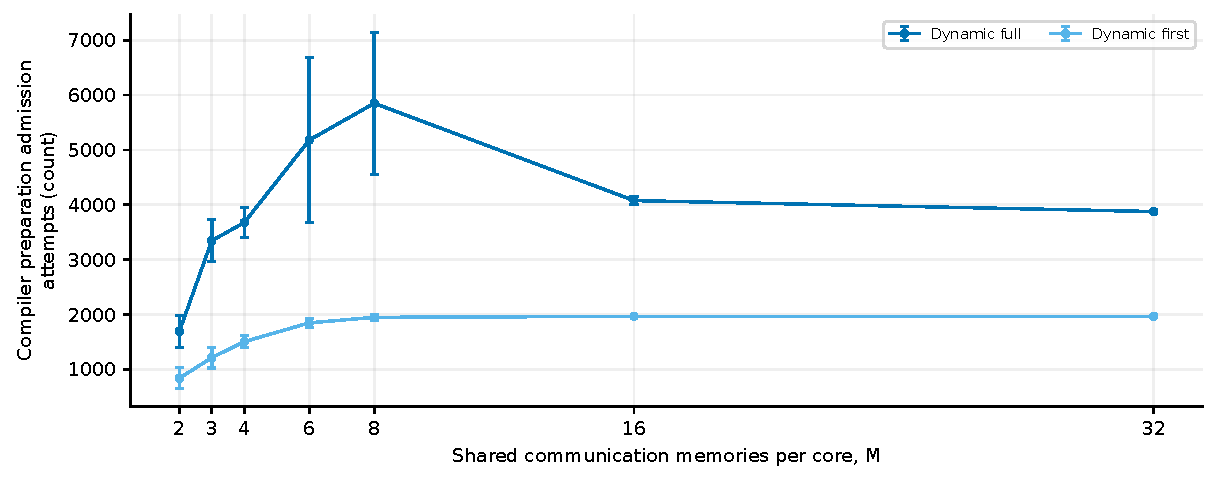
\includegraphics[width=.94\linewidth,height=.255\textheight,keepaspectratio]{figures/memory/mesh_shortest_reliable_runtime_admission_attempts.pdf}\captionof{figure}{Run-level mean and sample SD. Shared trace aliases are counted once.}\end{center}
\begin{center}{\scriptsize\setlength{\tabcolsep}{3pt}
\begin{tabular}{lrrrrr}
\toprule
M & ODG & CGP & ACGP & Dynamic full & Dynamic first \\
\midrule
2 & n/a & n/a & n/a & $1689.83\pm288.92$ & $834.00\pm190.08$ \\
3 & n/a & n/a & n/a & $3345.00\pm379.29$ & $1212.17\pm189.19$ \\
4 & n/a & n/a & n/a & $3676.00\pm273.67$ & $1502.67\pm113.90$ \\
6 & n/a & n/a & n/a & $5179.83\pm1502.58$ & $1845.83\pm76.55$ \\
8 & n/a & n/a & n/a & $5851.67\pm1294.63$ & $1946.50\pm49.09$ \\
16 & n/a & n/a & n/a & $4076.83\pm78.70$ & $1965.00\pm0.00$ \\
32 & n/a & n/a & n/a & $3876.00\pm0.00$ & $1965.00\pm0.00$ \\
\bottomrule\end{tabular}}
\captionof{table}{Mean $\pm$ sample SD; n/a denotes a metric outside that policy's instrumentation.}
{\footnotesize\href{https://github.com/sanjeevkrishnaa/Compiler-Driven-ACE/blob/codex/ace-scheduler-correctness/docs/latex/qft96_final/data/memory_mesh_shortest_reliable_runtime_admission_attempts.csv}{Exact CSV values and sample counts}}
\end{center}
\clearpage
\subsection*{Launched compiler preparations}
\begin{center}\includegraphics[width=.94\linewidth,height=.255\textheight,keepaspectratio]{figures/memory/mesh_shortest_reliable_runtime_launched_preparations.pdf}\captionof{figure}{Run-level mean and sample SD. Shared trace aliases are counted once.}\end{center}
\begin{center}{\scriptsize\setlength{\tabcolsep}{3pt}
\begin{tabular}{lrrrrr}
\toprule
M & ODG & CGP & ACGP & Dynamic full & Dynamic first \\
\midrule
2 & n/a & n/a & n/a & $903.67\pm26.24$ & $522.83\pm23.83$ \\
3 & n/a & n/a & n/a & $1736.50\pm35.84$ & $910.33\pm42.63$ \\
4 & n/a & n/a & n/a & $2362.67\pm44.62$ & $1293.67\pm29.38$ \\
6 & n/a & n/a & n/a & $3158.50\pm60.38$ & $1716.00\pm18.93$ \\
8 & n/a & n/a & n/a & $3527.50\pm56.72$ & $1879.17\pm13.35$ \\
16 & n/a & n/a & n/a & $3854.67\pm10.58$ & $1965.00\pm0.00$ \\
32 & n/a & n/a & n/a & $3876.00\pm0.00$ & $1965.00\pm0.00$ \\
\bottomrule\end{tabular}}
\captionof{table}{Mean $\pm$ sample SD; n/a denotes a metric outside that policy's instrumentation.}
{\footnotesize\href{https://github.com/sanjeevkrishnaa/Compiler-Driven-ACE/blob/codex/ace-scheduler-correctness/docs/latex/qft96_final/data/memory_mesh_shortest_reliable_runtime_launched_preparations.csv}{Exact CSV values and sample counts}}
\end{center}
\subsection*{Accepted compiler preparations}
\begin{center}\includegraphics[width=.94\linewidth,height=.255\textheight,keepaspectratio]{figures/memory/mesh_shortest_reliable_runtime_accepted_preparations.pdf}\captionof{figure}{Run-level mean and sample SD. Shared trace aliases are counted once.}\end{center}
\begin{center}{\scriptsize\setlength{\tabcolsep}{3pt}
\begin{tabular}{lrrrrr}
\toprule
M & ODG & CGP & ACGP & Dynamic full & Dynamic first \\
\midrule
2 & n/a & n/a & n/a & $870.33\pm33.96$ & $510.17\pm26.07$ \\
3 & n/a & n/a & n/a & $1558.50\pm32.49$ & $875.00\pm33.77$ \\
4 & n/a & n/a & n/a & $2188.33\pm31.39$ & $1261.00\pm22.38$ \\
6 & n/a & n/a & n/a & $2830.50\pm254.47$ & $1681.00\pm21.56$ \\
8 & n/a & n/a & n/a & $3146.83\pm205.87$ & $1863.00\pm21.43$ \\
16 & n/a & n/a & n/a & $3804.00\pm26.78$ & $1965.00\pm0.00$ \\
32 & n/a & n/a & n/a & $3876.00\pm0.00$ & $1965.00\pm0.00$ \\
\bottomrule\end{tabular}}
\captionof{table}{Mean $\pm$ sample SD; n/a denotes a metric outside that policy's instrumentation.}
{\footnotesize\href{https://github.com/sanjeevkrishnaa/Compiler-Driven-ACE/blob/codex/ace-scheduler-correctness/docs/latex/qft96_final/data/memory_mesh_shortest_reliable_runtime_accepted_preparations.csv}{Exact CSV values and sample counts}}
\end{center}
\clearpage
\subsection*{Rejected compiler preparations}
\begin{center}\includegraphics[width=.94\linewidth,height=.255\textheight,keepaspectratio]{figures/memory/mesh_shortest_reliable_runtime_rejected_preparations.pdf}\captionof{figure}{Run-level mean and sample SD. Shared trace aliases are counted once.}\end{center}
\begin{center}{\scriptsize\setlength{\tabcolsep}{3pt}
\begin{tabular}{lrrrrr}
\toprule
M & ODG & CGP & ACGP & Dynamic full & Dynamic first \\
\midrule
2 & n/a & n/a & n/a & $139.00\pm40.42$ & $72.833\pm38.603$ \\
3 & n/a & n/a & n/a & $317.50\pm62.48$ & $80.167\pm35.830$ \\
4 & n/a & n/a & n/a & $301.33\pm61.52$ & $63.833\pm24.871$ \\
6 & n/a & n/a & n/a & $481.00\pm288.04$ & $48.667\pm29.385$ \\
8 & n/a & n/a & n/a & $521.17\pm236.10$ & $22.667\pm19.054$ \\
16 & n/a & n/a & n/a & $82.167\pm27.147$ & $0.0000\pm0.0000$ \\
32 & n/a & n/a & n/a & $0.0000\pm0.0000$ & $0.0000\pm0.0000$ \\
\bottomrule\end{tabular}}
\captionof{table}{Mean $\pm$ sample SD; n/a denotes a metric outside that policy's instrumentation.}
{\footnotesize\href{https://github.com/sanjeevkrishnaa/Compiler-Driven-ACE/blob/codex/ace-scheduler-correctness/docs/latex/qft96_final/data/memory_mesh_shortest_reliable_runtime_rejected_preparations.csv}{Exact CSV values and sample counts}}
\end{center}
\subsection*{Compiler-ready request count}
\begin{center}\includegraphics[width=.94\linewidth,height=.255\textheight,keepaspectratio]{figures/memory/mesh_shortest_reliable_pregenerated_hits.pdf}\captionof{figure}{Run-level mean and sample SD. Shared trace aliases are counted once.}\end{center}
\begin{center}{\scriptsize\setlength{\tabcolsep}{3pt}
\begin{tabular}{lrrrrr}
\toprule
M & ODG & CGP & ACGP & Dynamic full & Dynamic first \\
\midrule
2 & n/a & n/a & n/a & $862.67\pm33.61$ & $503.33\pm26.06$ \\
3 & n/a & n/a & n/a & $1541.17\pm32.71$ & $860.67\pm32.18$ \\
4 & n/a & n/a & n/a & $2161.83\pm32.62$ & $1239.33\pm24.30$ \\
6 & n/a & n/a & n/a & $2777.17\pm261.05$ & $1645.83\pm22.49$ \\
8 & n/a & n/a & n/a & $3073.50\pm199.98$ & $1819.83\pm23.16$ \\
16 & n/a & n/a & n/a & $3708.00\pm18.97$ & $1914.83\pm6.11$ \\
32 & n/a & n/a & n/a & $3753.17\pm5.04$ & $1914.83\pm6.11$ \\
\bottomrule\end{tabular}}
\captionof{table}{Mean $\pm$ sample SD; n/a denotes a metric outside that policy's instrumentation.}
{\footnotesize\href{https://github.com/sanjeevkrishnaa/Compiler-Driven-ACE/blob/codex/ace-scheduler-correctness/docs/latex/qft96_final/data/memory_mesh_shortest_reliable_pregenerated_hits.csv}{Exact CSV values and sample counts}}
\end{center}
\clearpage
\subsection*{Intended compiler-hit count}
\begin{center}\includegraphics[width=.94\linewidth,height=.255\textheight,keepaspectratio]{figures/memory/mesh_shortest_reliable_intended_request_hits.pdf}\captionof{figure}{Run-level mean and sample SD. Shared trace aliases are counted once.}\end{center}
\begin{center}{\scriptsize\setlength{\tabcolsep}{3pt}
\begin{tabular}{lrrrrr}
\toprule
M & ODG & CGP & ACGP & Dynamic full & Dynamic first \\
\midrule
2 & n/a & n/a & n/a & $867.33\pm34.60$ & $507.50\pm27.16$ \\
3 & n/a & n/a & n/a & $1550.33\pm33.06$ & $868.83\pm33.05$ \\
4 & n/a & n/a & n/a & $2177.67\pm30.55$ & $1252.33\pm21.44$ \\
6 & n/a & n/a & n/a & $2809.17\pm259.78$ & $1666.00\pm24.29$ \\
8 & n/a & n/a & n/a & $3116.33\pm210.37$ & $1844.67\pm24.54$ \\
16 & n/a & n/a & n/a & $3764.67\pm25.51$ & $1945.17\pm5.78$ \\
32 & n/a & n/a & n/a & $3827.17\pm4.12$ & $1945.17\pm5.78$ \\
\bottomrule\end{tabular}}
\captionof{table}{Mean $\pm$ sample SD; n/a denotes a metric outside that policy's instrumentation.}
{\footnotesize\href{https://github.com/sanjeevkrishnaa/Compiler-Driven-ACE/blob/codex/ace-scheduler-correctness/docs/latex/qft96_final/data/memory_mesh_shortest_reliable_intended_request_hits.csv}{Exact CSV values and sample counts}}
\end{center}
\subsection*{Compiler-not-ready request count}
\begin{center}\includegraphics[width=.94\linewidth,height=.255\textheight,keepaspectratio]{figures/memory/mesh_shortest_reliable_compiler_not_ready_requests.pdf}\captionof{figure}{Run-level mean and sample SD. Shared trace aliases are counted once.}\end{center}
\begin{center}{\scriptsize\setlength{\tabcolsep}{3pt}
\begin{tabular}{lrrrrr}
\toprule
M & ODG & CGP & ACGP & Dynamic full & Dynamic first \\
\midrule
2 & n/a & n/a & n/a & $3013.33\pm33.61$ & $3372.67\pm26.06$ \\
3 & n/a & n/a & n/a & $2334.83\pm32.71$ & $3015.33\pm32.18$ \\
4 & n/a & n/a & n/a & $1714.17\pm32.62$ & $2636.67\pm24.30$ \\
6 & n/a & n/a & n/a & $1098.83\pm261.05$ & $2230.17\pm22.49$ \\
8 & n/a & n/a & n/a & $802.50\pm199.98$ & $2056.17\pm23.16$ \\
16 & n/a & n/a & n/a & $168.00\pm18.97$ & $1961.17\pm6.11$ \\
32 & n/a & n/a & n/a & $122.83\pm5.04$ & $1961.17\pm6.11$ \\
\bottomrule\end{tabular}}
\captionof{table}{Mean $\pm$ sample SD; n/a denotes a metric outside that policy's instrumentation.}
{\footnotesize\href{https://github.com/sanjeevkrishnaa/Compiler-Driven-ACE/blob/codex/ace-scheduler-correctness/docs/latex/qft96_final/data/memory_mesh_shortest_reliable_compiler_not_ready_requests.csv}{Exact CSV values and sample counts}}
\end{center}
\clearpage
\subsection*{Late compiler-pair uses}
\begin{center}\includegraphics[width=.94\linewidth,height=.255\textheight,keepaspectratio]{figures/memory/mesh_shortest_reliable_late_compiler_pair_uses.pdf}\captionof{figure}{Run-level mean and sample SD. Shared trace aliases are counted once.}\end{center}
\begin{center}{\scriptsize\setlength{\tabcolsep}{3pt}
\begin{tabular}{lrrrrr}
\toprule
M & ODG & CGP & ACGP & Dynamic full & Dynamic first \\
\midrule
2 & n/a & n/a & n/a & $4.667\pm2.582$ & $4.167\pm1.941$ \\
3 & n/a & n/a & n/a & $9.167\pm3.430$ & $8.167\pm2.137$ \\
4 & n/a & n/a & n/a & $15.833\pm3.251$ & $13.000\pm3.406$ \\
6 & n/a & n/a & n/a & $32.000\pm10.545$ & $20.167\pm6.178$ \\
8 & n/a & n/a & n/a & $42.833\pm12.561$ & $24.833\pm5.307$ \\
16 & n/a & n/a & n/a & $56.667\pm15.565$ & $30.333\pm5.854$ \\
32 & n/a & n/a & n/a & $74.000\pm5.797$ & $30.333\pm5.854$ \\
\bottomrule\end{tabular}}
\captionof{table}{Mean $\pm$ sample SD; n/a denotes a metric outside that policy's instrumentation.}
{\footnotesize\href{https://github.com/sanjeevkrishnaa/Compiler-Driven-ACE/blob/codex/ace-scheduler-correctness/docs/latex/qft96_final/data/memory_mesh_shortest_reliable_late_compiler_pair_uses.csv}{Exact CSV values and sample counts}}
\end{center}
\subsection*{Compiler fallback count}
\begin{center}\includegraphics[width=.94\linewidth,height=.255\textheight,keepaspectratio]{figures/memory/mesh_shortest_reliable_on_demand_fallbacks.pdf}\captionof{figure}{Run-level mean and sample SD. Shared trace aliases are counted once.}\end{center}
\begin{center}{\scriptsize\setlength{\tabcolsep}{3pt}
\begin{tabular}{lrrrrr}
\toprule
M & ODG & CGP & ACGP & Dynamic full & Dynamic first \\
\midrule
2 & n/a & n/a & n/a & $3008.67\pm34.60$ & $3368.50\pm27.16$ \\
3 & n/a & n/a & n/a & $2325.67\pm33.06$ & $3007.17\pm33.05$ \\
4 & n/a & n/a & n/a & $1698.33\pm30.55$ & $2623.67\pm21.44$ \\
6 & n/a & n/a & n/a & $1066.83\pm259.78$ & $2210.00\pm24.29$ \\
8 & n/a & n/a & n/a & $759.67\pm210.37$ & $2031.33\pm24.54$ \\
16 & n/a & n/a & n/a & $111.33\pm25.51$ & $1930.83\pm5.78$ \\
32 & n/a & n/a & n/a & $48.833\pm4.119$ & $1930.83\pm5.78$ \\
\bottomrule\end{tabular}}
\captionof{table}{Mean $\pm$ sample SD; n/a denotes a metric outside that policy's instrumentation.}
{\footnotesize\href{https://github.com/sanjeevkrishnaa/Compiler-Driven-ACE/blob/codex/ace-scheduler-correctness/docs/latex/qft96_final/data/memory_mesh_shortest_reliable_on_demand_fallbacks.csv}{Exact CSV values and sample counts}}
\end{center}
\clearpage
\subsection*{Generated compiler pairs}
\begin{center}\includegraphics[width=.94\linewidth,height=.255\textheight,keepaspectratio]{figures/memory/mesh_shortest_reliable_generated_compiler_pairs.pdf}\captionof{figure}{Run-level mean and sample SD. Shared trace aliases are counted once.}\end{center}
\begin{center}{\scriptsize\setlength{\tabcolsep}{3pt}
\begin{tabular}{lrrrrr}
\toprule
M & ODG & CGP & ACGP & Dynamic full & Dynamic first \\
\midrule
2 & n/a & n/a & n/a & $870.33\pm33.96$ & $510.17\pm26.07$ \\
3 & n/a & n/a & n/a & $1558.50\pm32.49$ & $875.00\pm33.77$ \\
4 & n/a & n/a & n/a & $2188.33\pm31.39$ & $1261.00\pm22.38$ \\
6 & n/a & n/a & n/a & $2830.50\pm254.47$ & $1681.00\pm21.56$ \\
8 & n/a & n/a & n/a & $3146.83\pm205.87$ & $1863.00\pm21.43$ \\
16 & n/a & n/a & n/a & $3804.00\pm26.78$ & $1965.00\pm0.00$ \\
32 & n/a & n/a & n/a & $3876.00\pm0.00$ & $1965.00\pm0.00$ \\
\bottomrule\end{tabular}}
\captionof{table}{Mean $\pm$ sample SD; n/a denotes a metric outside that policy's instrumentation.}
{\footnotesize\href{https://github.com/sanjeevkrishnaa/Compiler-Driven-ACE/blob/codex/ace-scheduler-correctness/docs/latex/qft96_final/data/memory_mesh_shortest_reliable_generated_compiler_pairs.csv}{Exact CSV values and sample counts}}
\end{center}
\subsection*{Used compiler pairs}
\begin{center}\includegraphics[width=.94\linewidth,height=.255\textheight,keepaspectratio]{figures/memory/mesh_shortest_reliable_utilized_compiler_pairs.pdf}\captionof{figure}{Run-level mean and sample SD. Shared trace aliases are counted once.}\end{center}
\begin{center}{\scriptsize\setlength{\tabcolsep}{3pt}
\begin{tabular}{lrrrrr}
\toprule
M & ODG & CGP & ACGP & Dynamic full & Dynamic first \\
\midrule
2 & n/a & n/a & n/a & $867.33\pm34.60$ & $507.50\pm27.16$ \\
3 & n/a & n/a & n/a & $1550.33\pm33.06$ & $868.83\pm33.05$ \\
4 & n/a & n/a & n/a & $2177.67\pm30.55$ & $1252.33\pm21.44$ \\
6 & n/a & n/a & n/a & $2809.17\pm259.78$ & $1666.00\pm24.29$ \\
8 & n/a & n/a & n/a & $3116.33\pm210.37$ & $1844.67\pm24.54$ \\
16 & n/a & n/a & n/a & $3764.67\pm25.51$ & $1945.17\pm5.78$ \\
32 & n/a & n/a & n/a & $3827.17\pm4.12$ & $1945.17\pm5.78$ \\
\bottomrule\end{tabular}}
\captionof{table}{Mean $\pm$ sample SD; n/a denotes a metric outside that policy's instrumentation.}
{\footnotesize\href{https://github.com/sanjeevkrishnaa/Compiler-Driven-ACE/blob/codex/ace-scheduler-correctness/docs/latex/qft96_final/data/memory_mesh_shortest_reliable_utilized_compiler_pairs.csv}{Exact CSV values and sample counts}}
\end{center}
\clearpage
\subsection*{Expired compiler pairs}
\begin{center}\includegraphics[width=.94\linewidth,height=.255\textheight,keepaspectratio]{figures/memory/mesh_shortest_reliable_expired_compiler_pairs.pdf}\captionof{figure}{Run-level mean and sample SD. Shared trace aliases are counted once.}\end{center}
\begin{center}{\scriptsize\setlength{\tabcolsep}{3pt}
\begin{tabular}{lrrrrr}
\toprule
M & ODG & CGP & ACGP & Dynamic full & Dynamic first \\
\midrule
2 & n/a & n/a & n/a & $0.8333\pm0.7528$ & $0.6667\pm0.8165$ \\
3 & n/a & n/a & n/a & $2.500\pm1.225$ & $1.333\pm1.211$ \\
4 & n/a & n/a & n/a & $2.000\pm1.265$ & $1.500\pm1.049$ \\
6 & n/a & n/a & n/a & $7.667\pm6.439$ & $3.000\pm2.608$ \\
8 & n/a & n/a & n/a & $12.000\pm5.550$ & $4.000\pm1.897$ \\
16 & n/a & n/a & n/a & $6.833\pm2.229$ & $4.500\pm2.074$ \\
32 & n/a & n/a & n/a & $6.833\pm2.317$ & $4.500\pm2.074$ \\
\bottomrule\end{tabular}}
\captionof{table}{Mean $\pm$ sample SD; n/a denotes a metric outside that policy's instrumentation.}
{\footnotesize\href{https://github.com/sanjeevkrishnaa/Compiler-Driven-ACE/blob/codex/ace-scheduler-correctness/docs/latex/qft96_final/data/memory_mesh_shortest_reliable_expired_compiler_pairs.csv}{Exact CSV values and sample counts}}
\end{center}
\subsection*{Remaining compiler pairs}
\begin{center}\includegraphics[width=.94\linewidth,height=.255\textheight,keepaspectratio]{figures/memory/mesh_shortest_reliable_remaining_compiler_pairs.pdf}\captionof{figure}{Run-level mean and sample SD. Shared trace aliases are counted once.}\end{center}
\begin{center}{\scriptsize\setlength{\tabcolsep}{3pt}
\begin{tabular}{lrrrrr}
\toprule
M & ODG & CGP & ACGP & Dynamic full & Dynamic first \\
\midrule
2 & n/a & n/a & n/a & $2.167\pm0.753$ & $2.000\pm1.265$ \\
3 & n/a & n/a & n/a & $5.667\pm1.033$ & $4.833\pm1.941$ \\
4 & n/a & n/a & n/a & $8.667\pm2.066$ & $7.167\pm1.602$ \\
6 & n/a & n/a & n/a & $13.667\pm2.338$ & $12.000\pm2.530$ \\
8 & n/a & n/a & n/a & $18.500\pm3.507$ & $14.333\pm2.875$ \\
16 & n/a & n/a & n/a & $32.500\pm6.058$ & $15.333\pm4.502$ \\
32 & n/a & n/a & n/a & $42.000\pm4.940$ & $15.333\pm4.502$ \\
\bottomrule\end{tabular}}
\captionof{table}{Mean $\pm$ sample SD; n/a denotes a metric outside that policy's instrumentation.}
{\footnotesize\href{https://github.com/sanjeevkrishnaa/Compiler-Driven-ACE/blob/codex/ace-scheduler-correctness/docs/latex/qft96_final/data/memory_mesh_shortest_reliable_remaining_compiler_pairs.csv}{Exact CSV values and sample counts}}
\end{center}
\clearpage
\subsection*{Compiler fidelity at creation}
\begin{center}\includegraphics[width=.94\linewidth,height=.255\textheight,keepaspectratio]{figures/memory/mesh_shortest_reliable_average_fidelity_at_creation.pdf}\captionof{figure}{Run-level mean and sample SD. Shared trace aliases are counted once.}\end{center}
\begin{center}{\scriptsize\setlength{\tabcolsep}{3pt}
\begin{tabular}{lrrrrr}
\toprule
M & ODG & CGP & ACGP & Dynamic full & Dynamic first \\
\midrule
2 & n/a & n/a & n/a & $0.9498\pm0.0000$ & $0.9498\pm0.0000$ \\
3 & n/a & n/a & n/a & $0.9498\pm0.0000$ & $0.9498\pm0.0000$ \\
4 & n/a & n/a & n/a & $0.9498\pm0.0000$ & $0.9498\pm0.0000$ \\
6 & n/a & n/a & n/a & $0.9498\pm0.0000$ & $0.9498\pm0.0000$ \\
8 & n/a & n/a & n/a & $0.9498\pm0.0000$ & $0.9498\pm0.0000$ \\
16 & n/a & n/a & n/a & $0.9498\pm0.0000$ & $0.9498\pm0.0000$ \\
32 & n/a & n/a & n/a & $0.9498\pm0.0000$ & $0.9498\pm0.0000$ \\
\bottomrule\end{tabular}}
\captionof{table}{Mean $\pm$ sample SD; n/a denotes a metric outside that policy's instrumentation.}
{\footnotesize\href{https://github.com/sanjeevkrishnaa/Compiler-Driven-ACE/blob/codex/ace-scheduler-correctness/docs/latex/qft96_final/data/memory_mesh_shortest_reliable_average_fidelity_at_creation.csv}{Exact CSV values and sample counts}}
\end{center}
\subsection*{Compiler fidelity at use}
\begin{center}\includegraphics[width=.94\linewidth,height=.255\textheight,keepaspectratio]{figures/memory/mesh_shortest_reliable_average_fidelity_at_utilization.pdf}\captionof{figure}{Run-level mean and sample SD. Shared trace aliases are counted once.}\end{center}
\begin{center}{\scriptsize\setlength{\tabcolsep}{3pt}
\begin{tabular}{lrrrrr}
\toprule
M & ODG & CGP & ACGP & Dynamic full & Dynamic first \\
\midrule
2 & n/a & n/a & n/a & $0.9360\pm0.0002$ & $0.9414\pm0.0001$ \\
3 & n/a & n/a & n/a & $0.9378\pm0.0003$ & $0.9417\pm0.0001$ \\
4 & n/a & n/a & n/a & $0.9394\pm0.0001$ & $0.9423\pm0.0000$ \\
6 & n/a & n/a & n/a & $0.9403\pm0.0004$ & $0.9424\pm0.0001$ \\
8 & n/a & n/a & n/a & $0.9408\pm0.0004$ & $0.9425\pm0.0000$ \\
16 & n/a & n/a & n/a & $0.9419\pm0.0000$ & $0.9425\pm0.0000$ \\
32 & n/a & n/a & n/a & $0.9421\pm0.0000$ & $0.9425\pm0.0000$ \\
\bottomrule\end{tabular}}
\captionof{table}{Mean $\pm$ sample SD; n/a denotes a metric outside that policy's instrumentation.}
{\footnotesize\href{https://github.com/sanjeevkrishnaa/Compiler-Driven-ACE/blob/codex/ace-scheduler-correctness/docs/latex/qft96_final/data/memory_mesh_shortest_reliable_average_fidelity_at_utilization.csv}{Exact CSV values and sample counts}}
\end{center}
\clearpage
\subsection*{Mean layer latency}
\begin{center}\includegraphics[width=.94\linewidth,height=.255\textheight,keepaspectratio]{figures/memory/mesh_shortest_reliable_avg_layer_latency_ms.pdf}\captionof{figure}{Run-level mean and sample SD. Shared trace aliases are counted once.}\end{center}
\begin{center}{\scriptsize\setlength{\tabcolsep}{3pt}
\begin{tabular}{lrrrrr}
\toprule
M & ODG & CGP & ACGP & Dynamic full & Dynamic first \\
\midrule
2 & $2.069\pm0.050$ & $2.896\pm0.040$ & $2.897\pm0.032$ & $2.641\pm0.082$ & $2.150\pm0.084$ \\
3 & $1.838\pm0.034$ & $2.460\pm0.085$ & $2.419\pm0.112$ & $2.131\pm0.077$ & $1.822\pm0.051$ \\
4 & $1.787\pm0.038$ & $2.105\pm0.091$ & $2.041\pm0.078$ & $1.702\pm0.040$ & $1.684\pm0.034$ \\
6 & $1.767\pm0.028$ & $1.595\pm0.068$ & $1.609\pm0.070$ & $1.353\pm0.211$ & $1.553\pm0.031$ \\
8 & $1.770\pm0.022$ & $1.439\pm0.051$ & $1.410\pm0.053$ & $1.186\pm0.215$ & $1.499\pm0.045$ \\
16 & $1.770\pm0.022$ & $1.176\pm0.039$ & $1.164\pm0.051$ & $0.6470\pm0.0254$ & $1.461\pm0.046$ \\
32 & $1.770\pm0.022$ & $1.108\pm0.056$ & $1.123\pm0.043$ & $0.5671\pm0.0031$ & $1.461\pm0.046$ \\
\bottomrule\end{tabular}}
\captionof{table}{Mean $\pm$ sample SD; n/a denotes a metric outside that policy's instrumentation.}
{\footnotesize\href{https://github.com/sanjeevkrishnaa/Compiler-Driven-ACE/blob/codex/ace-scheduler-correctness/docs/latex/qft96_final/data/memory_mesh_shortest_reliable_avg_layer_latency_ms.csv}{Exact CSV values and sample counts}}
\end{center}
\subsection*{Maximum layer latency}
\begin{center}\includegraphics[width=.94\linewidth,height=.255\textheight,keepaspectratio]{figures/memory/mesh_shortest_reliable_max_layer_latency_ms.pdf}\captionof{figure}{Run-level mean and sample SD. Shared trace aliases are counted once.}\end{center}
\begin{center}{\scriptsize\setlength{\tabcolsep}{3pt}
\begin{tabular}{lrrrrr}
\toprule
M & ODG & CGP & ACGP & Dynamic full & Dynamic first \\
\midrule
2 & $15.550\pm1.408$ & $25.527\pm2.109$ & $24.296\pm1.387$ & $22.601\pm2.685$ & $17.267\pm1.320$ \\
3 & $15.184\pm1.042$ & $27.034\pm14.738$ & $21.817\pm2.120$ & $19.384\pm2.499$ & $14.150\pm1.559$ \\
4 & $13.667\pm1.159$ & $25.444\pm14.897$ & $20.276\pm4.452$ & $15.917\pm0.627$ & $13.467\pm0.855$ \\
6 & $13.600\pm1.108$ & $21.640\pm16.826$ & $16.834\pm2.204$ & $14.050\pm2.197$ & $13.534\pm0.747$ \\
8 & $14.217\pm0.842$ & $14.664\pm2.007$ & $14.266\pm2.220$ & $15.584\pm5.209$ & $12.467\pm1.435$ \\
16 & $14.217\pm0.842$ & $10.117\pm1.850$ & $9.650\pm0.874$ & $7.417\pm0.757$ & $12.750\pm1.294$ \\
32 & $14.217\pm0.842$ & $8.517\pm0.467$ & $8.600\pm0.310$ & $4.133\pm0.761$ & $12.750\pm1.294$ \\
\bottomrule\end{tabular}}
\captionof{table}{Mean $\pm$ sample SD; n/a denotes a metric outside that policy's instrumentation.}
{\footnotesize\href{https://github.com/sanjeevkrishnaa/Compiler-Driven-ACE/blob/codex/ace-scheduler-correctness/docs/latex/qft96_final/data/memory_mesh_shortest_reliable_max_layer_latency_ms.csv}{Exact CSV values and sample counts}}
\end{center}
\clearpage
\subsection*{Minimum layer latency}
\begin{center}\includegraphics[width=.94\linewidth,height=.255\textheight,keepaspectratio]{figures/memory/mesh_shortest_reliable_min_layer_latency_ms.pdf}\captionof{figure}{Run-level mean and sample SD. Shared trace aliases are counted once.}\end{center}
\begin{center}{\scriptsize\setlength{\tabcolsep}{3pt}
\begin{tabular}{lrrrrr}
\toprule
M & ODG & CGP & ACGP & Dynamic full & Dynamic first \\
\midrule
2 & $0.0000\pm0.0000$ & $0.0000\pm0.0000$ & $0.0000\pm0.0000$ & $0.0000\pm0.0000$ & $0.0000\pm0.0000$ \\
3 & $0.0000\pm0.0000$ & $0.0000\pm0.0000$ & $0.0000\pm0.0000$ & $0.0000\pm0.0000$ & $0.0000\pm0.0000$ \\
4 & $0.0000\pm0.0000$ & $0.0000\pm0.0000$ & $0.0000\pm0.0000$ & $0.0000\pm0.0000$ & $0.0000\pm0.0000$ \\
6 & $0.0000\pm0.0000$ & $0.0000\pm0.0000$ & $0.0000\pm0.0000$ & $0.0000\pm0.0000$ & $0.0000\pm0.0000$ \\
8 & $0.0000\pm0.0000$ & $0.0000\pm0.0000$ & $0.0000\pm0.0000$ & $0.0000\pm0.0000$ & $0.0000\pm0.0000$ \\
16 & $0.0000\pm0.0000$ & $0.0000\pm0.0000$ & $0.0000\pm0.0000$ & $0.0000\pm0.0000$ & $0.0000\pm0.0000$ \\
32 & $0.0000\pm0.0000$ & $0.0000\pm0.0000$ & $0.0000\pm0.0000$ & $0.0000\pm0.0000$ & $0.0000\pm0.0000$ \\
\bottomrule\end{tabular}}
\captionof{table}{Mean $\pm$ sample SD; n/a denotes a metric outside that policy's instrumentation.}
{\footnotesize\href{https://github.com/sanjeevkrishnaa/Compiler-Driven-ACE/blob/codex/ace-scheduler-correctness/docs/latex/qft96_final/data/memory_mesh_shortest_reliable_min_layer_latency_ms.csv}{Exact CSV values and sample counts}}
\end{center}
\section{Max Reliability}
\clearpage
\subsection*{Mean request latency}
\begin{center}\includegraphics[width=.94\linewidth,height=.255\textheight,keepaspectratio]{figures/memory/mesh_max_reliability_request_latency_mean_ms.pdf}\captionof{figure}{Run-level mean and sample SD. Shared trace aliases are counted once.}\end{center}
\begin{center}{\scriptsize\setlength{\tabcolsep}{3pt}
\begin{tabular}{lrrrrr}
\toprule
M & ODG & CGP & ACGP & Dynamic full & Dynamic first \\
\midrule
2 & $1.871\pm0.106$ & $3.111\pm0.170$ & $3.120\pm0.130$ & $2.813\pm0.145$ & $1.926\pm0.084$ \\
3 & $1.479\pm0.057$ & $2.580\pm0.153$ & $2.519\pm0.165$ & $2.182\pm0.213$ & $1.450\pm0.056$ \\
4 & $1.362\pm0.032$ & $2.183\pm0.142$ & $2.162\pm0.120$ & $1.693\pm0.164$ & $1.257\pm0.083$ \\
6 & $1.326\pm0.014$ & $1.745\pm0.088$ & $1.701\pm0.085$ & $1.296\pm0.090$ & $1.086\pm0.056$ \\
8 & $1.322\pm0.011$ & $1.546\pm0.066$ & $1.504\pm0.085$ & $0.9469\pm0.1370$ & $1.024\pm0.061$ \\
16 & $1.322\pm0.012$ & $1.217\pm0.061$ & $1.262\pm0.042$ & $0.5912\pm0.1245$ & $0.9715\pm0.0476$ \\
32 & $1.322\pm0.012$ & $1.188\pm0.027$ & $1.215\pm0.029$ & $0.4599\pm0.0011$ & $0.9706\pm0.0465$ \\
\bottomrule\end{tabular}}
\captionof{table}{Mean $\pm$ sample SD; n/a denotes a metric outside that policy's instrumentation.}
{\footnotesize\href{https://github.com/sanjeevkrishnaa/Compiler-Driven-ACE/blob/codex/ace-scheduler-correctness/docs/latex/qft96_final/data/memory_mesh_max_reliability_request_latency_mean_ms.csv}{Exact CSV values and sample counts}}
\end{center}
\subsection*{Median request latency}
\begin{center}\includegraphics[width=.94\linewidth,height=.255\textheight,keepaspectratio]{figures/memory/mesh_max_reliability_request_latency_median_ms.pdf}\captionof{figure}{Run-level mean and sample SD. Shared trace aliases are counted once.}\end{center}
\begin{center}{\scriptsize\setlength{\tabcolsep}{3pt}
\begin{tabular}{lrrrrr}
\toprule
M & ODG & CGP & ACGP & Dynamic full & Dynamic first \\
\midrule
2 & $1.583\pm0.147$ & $2.450\pm0.176$ & $2.467\pm0.186$ & $2.083\pm0.183$ & $1.617\pm0.117$ \\
3 & $1.200\pm0.000$ & $2.017\pm0.133$ & $1.933\pm0.186$ & $1.567\pm0.137$ & $1.183\pm0.041$ \\
4 & $1.117\pm0.098$ & $1.650\pm0.122$ & $1.617\pm0.075$ & $1.117\pm0.133$ & $1.000\pm0.063$ \\
6 & $1.033\pm0.082$ & $1.333\pm0.082$ & $1.254\pm0.157$ & $0.7500\pm0.0837$ & $0.7000\pm0.0000$ \\
8 & $1.000\pm0.000$ & $1.117\pm0.098$ & $1.150\pm0.122$ & $0.5167\pm0.0408$ & $0.6667\pm0.0516$ \\
16 & $1.033\pm0.082$ & $0.9667\pm0.0516$ & $0.9833\pm0.0408$ & $0.5000\pm0.0000$ & $0.6333\pm0.0516$ \\
32 & $1.033\pm0.082$ & $0.9167\pm0.0408$ & $0.9333\pm0.0516$ & $0.5000\pm0.0000$ & $0.6333\pm0.0516$ \\
\bottomrule\end{tabular}}
\captionof{table}{Mean $\pm$ sample SD; n/a denotes a metric outside that policy's instrumentation.}
{\footnotesize\href{https://github.com/sanjeevkrishnaa/Compiler-Driven-ACE/blob/codex/ace-scheduler-correctness/docs/latex/qft96_final/data/memory_mesh_max_reliability_request_latency_median_ms.csv}{Exact CSV values and sample counts}}
\end{center}
\clearpage
\subsection*{p95 request latency}
\begin{center}\includegraphics[width=.94\linewidth,height=.255\textheight,keepaspectratio]{figures/memory/mesh_max_reliability_request_latency_p95_ms.pdf}\captionof{figure}{Run-level mean and sample SD. Shared trace aliases are counted once.}\end{center}
\begin{center}{\scriptsize\setlength{\tabcolsep}{3pt}
\begin{tabular}{lrrrrr}
\toprule
M & ODG & CGP & ACGP & Dynamic full & Dynamic first \\
\midrule
2 & $4.350\pm0.315$ & $8.017\pm0.741$ & $8.100\pm0.465$ & $7.600\pm0.395$ & $4.583\pm0.240$ \\
3 & $3.383\pm0.248$ & $6.767\pm0.493$ & $6.567\pm0.446$ & $6.233\pm0.742$ & $3.417\pm0.194$ \\
4 & $3.200\pm0.000$ & $5.900\pm0.551$ & $5.956\pm0.585$ & $5.033\pm0.509$ & $3.100\pm0.155$ \\
6 & $3.200\pm0.000$ & $4.584\pm0.407$ & $4.562\pm0.291$ & $3.967\pm0.532$ & $2.800\pm0.155$ \\
8 & $3.167\pm0.082$ & $4.150\pm0.362$ & $3.883\pm0.331$ & $2.800\pm0.593$ & $2.683\pm0.041$ \\
16 & $3.167\pm0.082$ & $2.900\pm0.322$ & $2.983\pm0.256$ & $1.283\pm0.744$ & $2.600\pm0.200$ \\
32 & $3.167\pm0.082$ & $2.785\pm0.223$ & $2.933\pm0.250$ & $0.5000\pm0.0000$ & $2.600\pm0.200$ \\
\bottomrule\end{tabular}}
\captionof{table}{Mean $\pm$ sample SD; n/a denotes a metric outside that policy's instrumentation.}
{\footnotesize\href{https://github.com/sanjeevkrishnaa/Compiler-Driven-ACE/blob/codex/ace-scheduler-correctness/docs/latex/qft96_final/data/memory_mesh_max_reliability_request_latency_p95_ms.csv}{Exact CSV values and sample counts}}
\end{center}
\subsection*{Maximum request latency}
\begin{center}\includegraphics[width=.94\linewidth,height=.255\textheight,keepaspectratio]{figures/memory/mesh_max_reliability_request_latency_max_ms.pdf}\captionof{figure}{Run-level mean and sample SD. Shared trace aliases are counted once.}\end{center}
\begin{center}{\scriptsize\setlength{\tabcolsep}{3pt}
\begin{tabular}{lrrrrr}
\toprule
M & ODG & CGP & ACGP & Dynamic full & Dynamic first \\
\midrule
2 & $9.700\pm0.795$ & $16.011\pm1.439$ & $16.417\pm3.024$ & $18.067\pm2.242$ & $10.750\pm1.537$ \\
3 & $9.367\pm0.774$ & $14.845\pm2.030$ & $20.793\pm16.325$ & $14.584\pm1.699$ & $9.917\pm1.155$ \\
4 & $8.467\pm0.973$ & $19.999\pm15.855$ & $12.950\pm1.549$ & $12.167\pm1.598$ & $9.634\pm1.322$ \\
6 & $9.034\pm1.033$ & $10.734\pm2.270$ & $11.049\pm1.642$ & $11.350\pm1.358$ & $8.550\pm1.164$ \\
8 & $9.200\pm1.000$ & $30.659\pm23.276$ & $10.061\pm2.307$ & $9.617\pm1.777$ & $8.034\pm1.211$ \\
16 & $9.200\pm1.000$ & $5.752\pm0.612$ & $6.450\pm1.154$ & $7.267\pm4.016$ & $8.300\pm0.959$ \\
32 & $9.200\pm1.000$ & $5.083\pm0.546$ & $5.183\pm0.564$ & $2.850\pm0.251$ & $8.317\pm0.947$ \\
\bottomrule\end{tabular}}
\captionof{table}{Mean $\pm$ sample SD; n/a denotes a metric outside that policy's instrumentation.}
{\footnotesize\href{https://github.com/sanjeevkrishnaa/Compiler-Driven-ACE/blob/codex/ace-scheduler-correctness/docs/latex/qft96_final/data/memory_mesh_max_reliability_request_latency_max_ms.csv}{Exact CSV values and sample counts}}
\end{center}
\clearpage
\subsection*{Communication makespan}
\begin{center}\includegraphics[width=.94\linewidth,height=.255\textheight,keepaspectratio]{figures/memory/mesh_max_reliability_end_to_end_latency_ms.pdf}\captionof{figure}{Run-level mean and sample SD. Shared trace aliases are counted once.}\end{center}
\begin{center}{\scriptsize\setlength{\tabcolsep}{3pt}
\begin{tabular}{lrrrrr}
\toprule
M & ODG & CGP & ACGP & Dynamic full & Dynamic first \\
\midrule
2 & $4.670\pm0.244$ & $5.434\pm0.345$ & $5.429\pm0.336$ & $5.201\pm0.288$ & $4.681\pm0.237$ \\
3 & $4.401\pm0.195$ & $5.002\pm0.323$ & $4.956\pm0.301$ & $4.737\pm0.266$ & $4.367\pm0.186$ \\
4 & $4.321\pm0.164$ & $4.661\pm0.244$ & $4.598\pm0.214$ & $4.390\pm0.214$ & $4.256\pm0.188$ \\
6 & $4.308\pm0.157$ & $4.260\pm0.220$ & $4.240\pm0.183$ & $4.104\pm0.132$ & $4.154\pm0.177$ \\
8 & $4.297\pm0.144$ & $4.096\pm0.165$ & $4.020\pm0.174$ & $3.781\pm0.178$ & $4.106\pm0.175$ \\
16 & $4.302\pm0.150$ & $3.781\pm0.135$ & $3.799\pm0.117$ & $3.365\pm0.172$ & $4.077\pm0.174$ \\
32 & $4.302\pm0.150$ & $3.744\pm0.114$ & $3.748\pm0.109$ & $3.206\pm0.055$ & $4.083\pm0.182$ \\
\bottomrule\end{tabular}}
\captionof{table}{Mean $\pm$ sample SD; n/a denotes a metric outside that policy's instrumentation.}
{\footnotesize\href{https://github.com/sanjeevkrishnaa/Compiler-Driven-ACE/blob/codex/ace-scheduler-correctness/docs/latex/qft96_final/data/memory_mesh_max_reliability_end_to_end_latency_ms.csv}{Exact CSV values and sample counts}}
\end{center}
\subsection*{Mean admission wait}
\begin{center}\includegraphics[width=.94\linewidth,height=.255\textheight,keepaspectratio]{figures/memory/mesh_max_reliability_average_admission_wait_ms.pdf}\captionof{figure}{Run-level mean and sample SD. Shared trace aliases are counted once.}\end{center}
\begin{center}{\scriptsize\setlength{\tabcolsep}{3pt}
\begin{tabular}{lrrrrr}
\toprule
M & ODG & CGP & ACGP & Dynamic full & Dynamic first \\
\midrule
2 & $0.5628\pm0.1018$ & $2.028\pm0.165$ & $2.060\pm0.129$ & $1.671\pm0.127$ & $0.6942\pm0.0683$ \\
3 & $0.1644\pm0.0510$ & $1.677\pm0.144$ & $1.639\pm0.161$ & $1.167\pm0.189$ & $0.2639\pm0.0227$ \\
4 & $0.0435\pm0.0225$ & $1.408\pm0.144$ & $1.426\pm0.129$ & $0.7779\pm0.1230$ & $0.1357\pm0.0479$ \\
6 & $0.0033\pm0.0041$ & $1.124\pm0.070$ & $1.095\pm0.092$ & $0.5119\pm0.0809$ & $0.0361\pm0.0031$ \\
8 & $0.0001\pm0.0002$ & $0.9793\pm0.0615$ & $0.9670\pm0.0816$ & $0.2984\pm0.0995$ & $0.0161\pm0.0108$ \\
16 & $0.0000\pm0.0000$ & $0.7450\pm0.0555$ & $0.7962\pm0.0387$ & $0.0921\pm0.0910$ & $0.0000\pm0.0000$ \\
32 & $0.0000\pm0.0000$ & $0.7251\pm0.0290$ & $0.7561\pm0.0267$ & $0.0001\pm0.0002$ & $0.0000\pm0.0000$ \\
\bottomrule\end{tabular}}
\captionof{table}{Mean $\pm$ sample SD; n/a denotes a metric outside that policy's instrumentation.}
{\footnotesize\href{https://github.com/sanjeevkrishnaa/Compiler-Driven-ACE/blob/codex/ace-scheduler-correctness/docs/latex/qft96_final/data/memory_mesh_max_reliability_average_admission_wait_ms.csv}{Exact CSV values and sample counts}}
\end{center}
\clearpage
\subsection*{Delivered EPR fidelity}
\begin{center}\includegraphics[width=.94\linewidth,height=.255\textheight,keepaspectratio]{figures/memory/mesh_max_reliability_average_delivered_epr_fidelity.pdf}\captionof{figure}{Run-level mean and sample SD. Shared trace aliases are counted once.}\end{center}
\begin{center}{\scriptsize\setlength{\tabcolsep}{3pt}
\begin{tabular}{lrrrrr}
\toprule
M & ODG & CGP & ACGP & Dynamic full & Dynamic first \\
\midrule
2 & $0.9498\pm0.0000$ & $0.9426\pm0.0007$ & $0.9417\pm0.0009$ & $0.9468\pm0.0002$ & $0.9491\pm0.0002$ \\
3 & $0.9498\pm0.0000$ & $0.9371\pm0.0016$ & $0.9361\pm0.0012$ & $0.9451\pm0.0003$ & $0.9486\pm0.0003$ \\
4 & $0.9498\pm0.0000$ & $0.9334\pm0.0020$ & $0.9321\pm0.0018$ & $0.9442\pm0.0002$ & $0.9481\pm0.0004$ \\
6 & $0.9498\pm0.0000$ & $0.9287\pm0.0022$ & $0.9280\pm0.0022$ & $0.9432\pm0.0002$ & $0.9474\pm0.0004$ \\
8 & $0.9498\pm0.0000$ & $0.9263\pm0.0024$ & $0.9256\pm0.0020$ & $0.9423\pm0.0002$ & $0.9471\pm0.0004$ \\
16 & $0.9498\pm0.0000$ & $0.9236\pm0.0016$ & $0.9232\pm0.0015$ & $0.9417\pm0.0002$ & $0.9467\pm0.0004$ \\
32 & $0.9498\pm0.0000$ & $0.9240\pm0.0015$ & $0.9237\pm0.0016$ & $0.9418\pm0.0001$ & $0.9467\pm0.0003$ \\
\bottomrule\end{tabular}}
\captionof{table}{Mean $\pm$ sample SD; n/a denotes a metric outside that policy's instrumentation.}
{\footnotesize\href{https://github.com/sanjeevkrishnaa/Compiler-Driven-ACE/blob/codex/ace-scheduler-correctness/docs/latex/qft96_final/data/memory_mesh_max_reliability_average_delivered_epr_fidelity.csv}{Exact CSV values and sample counts}}
\end{center}
\subsection*{Compiler readiness fraction}
\begin{center}\includegraphics[width=.94\linewidth,height=.255\textheight,keepaspectratio]{figures/memory/mesh_max_reliability_pregenerated_success_rate.pdf}\captionof{figure}{Run-level mean and sample SD. Shared trace aliases are counted once.}\end{center}
\begin{center}{\scriptsize\setlength{\tabcolsep}{3pt}
\begin{tabular}{lrrrrr}
\toprule
M & ODG & CGP & ACGP & Dynamic full & Dynamic first \\
\midrule
2 & n/a & n/a & n/a & $0.1851\pm0.0189$ & $0.0860\pm0.0191$ \\
3 & n/a & n/a & n/a & $0.3381\pm0.0332$ & $0.1475\pm0.0353$ \\
4 & n/a & n/a & n/a & $0.4564\pm0.0549$ & $0.2219\pm0.0499$ \\
6 & n/a & n/a & n/a & $0.6067\pm0.0344$ & $0.3113\pm0.0575$ \\
8 & n/a & n/a & n/a & $0.7621\pm0.0552$ & $0.3588\pm0.0561$ \\
16 & n/a & n/a & n/a & $0.9331\pm0.0371$ & $0.4024\pm0.0452$ \\
32 & n/a & n/a & n/a & $0.9739\pm0.0032$ & $0.4041\pm0.0429$ \\
\bottomrule\end{tabular}}
\captionof{table}{Mean $\pm$ sample SD; n/a denotes a metric outside that policy's instrumentation.}
{\footnotesize\href{https://github.com/sanjeevkrishnaa/Compiler-Driven-ACE/blob/codex/ace-scheduler-correctness/docs/latex/qft96_final/data/memory_mesh_max_reliability_pregenerated_success_rate.csv}{Exact CSV values and sample counts}}
\end{center}
\clearpage
\subsection*{Intended compiler-hit fraction}
\begin{center}\includegraphics[width=.94\linewidth,height=.255\textheight,keepaspectratio]{figures/memory/mesh_max_reliability_intended_request_hit_rate.pdf}\captionof{figure}{Run-level mean and sample SD. Shared trace aliases are counted once.}\end{center}
\begin{center}{\scriptsize\setlength{\tabcolsep}{3pt}
\begin{tabular}{lrrrrr}
\toprule
M & ODG & CGP & ACGP & Dynamic full & Dynamic first \\
\midrule
2 & n/a & n/a & n/a & $0.1860\pm0.0187$ & $0.0868\pm0.0190$ \\
3 & n/a & n/a & n/a & $0.3402\pm0.0331$ & $0.1491\pm0.0354$ \\
4 & n/a & n/a & n/a & $0.4600\pm0.0554$ & $0.2246\pm0.0509$ \\
6 & n/a & n/a & n/a & $0.6131\pm0.0337$ & $0.3149\pm0.0579$ \\
8 & n/a & n/a & n/a & $0.7693\pm0.0550$ & $0.3634\pm0.0571$ \\
16 & n/a & n/a & n/a & $0.9461\pm0.0363$ & $0.4078\pm0.0461$ \\
32 & n/a & n/a & n/a & $0.9887\pm0.0022$ & $0.4096\pm0.0437$ \\
\bottomrule\end{tabular}}
\captionof{table}{Mean $\pm$ sample SD; n/a denotes a metric outside that policy's instrumentation.}
{\footnotesize\href{https://github.com/sanjeevkrishnaa/Compiler-Driven-ACE/blob/codex/ace-scheduler-correctness/docs/latex/qft96_final/data/memory_mesh_max_reliability_intended_request_hit_rate.csv}{Exact CSV values and sample counts}}
\end{center}
\subsection*{Compiler fallback fraction}
\begin{center}\includegraphics[width=.94\linewidth,height=.255\textheight,keepaspectratio]{figures/memory/mesh_max_reliability_on_demand_fallback_rate.pdf}\captionof{figure}{Run-level mean and sample SD. Shared trace aliases are counted once.}\end{center}
\begin{center}{\scriptsize\setlength{\tabcolsep}{3pt}
\begin{tabular}{lrrrrr}
\toprule
M & ODG & CGP & ACGP & Dynamic full & Dynamic first \\
\midrule
2 & n/a & n/a & n/a & $0.8140\pm0.0187$ & $0.9132\pm0.0190$ \\
3 & n/a & n/a & n/a & $0.6598\pm0.0331$ & $0.8509\pm0.0354$ \\
4 & n/a & n/a & n/a & $0.5400\pm0.0554$ & $0.7754\pm0.0509$ \\
6 & n/a & n/a & n/a & $0.3869\pm0.0337$ & $0.6851\pm0.0579$ \\
8 & n/a & n/a & n/a & $0.2307\pm0.0550$ & $0.6366\pm0.0571$ \\
16 & n/a & n/a & n/a & $0.0539\pm0.0363$ & $0.5922\pm0.0461$ \\
32 & n/a & n/a & n/a & $0.0113\pm0.0022$ & $0.5904\pm0.0437$ \\
\bottomrule\end{tabular}}
\captionof{table}{Mean $\pm$ sample SD; n/a denotes a metric outside that policy's instrumentation.}
{\footnotesize\href{https://github.com/sanjeevkrishnaa/Compiler-Driven-ACE/blob/codex/ace-scheduler-correctness/docs/latex/qft96_final/data/memory_mesh_max_reliability_on_demand_fallback_rate.csv}{Exact CSV values and sample counts}}
\end{center}
\clearpage
\subsection*{Compiler-cache waste}
\begin{center}\includegraphics[width=.94\linewidth,height=.255\textheight,keepaspectratio]{figures/memory/mesh_max_reliability_compiler_waste_percentage.pdf}\captionof{figure}{Run-level mean and sample SD. Shared trace aliases are counted once.}\end{center}
\begin{center}{\scriptsize\setlength{\tabcolsep}{3pt}
\begin{tabular}{lrrrrr}
\toprule
M & ODG & CGP & ACGP & Dynamic full & Dynamic first \\
\midrule
2 & n/a & n/a & n/a & $0.2909\pm0.1762$ & $0.4889\pm0.1457$ \\
3 & n/a & n/a & n/a & $0.4037\pm0.1473$ & $0.5999\pm0.3993$ \\
4 & n/a & n/a & n/a & $0.5427\pm0.1146$ & $0.9258\pm0.2332$ \\
6 & n/a & n/a & n/a & $0.7204\pm0.2535$ & $0.8570\pm0.1323$ \\
8 & n/a & n/a & n/a & $0.6827\pm0.1275$ & $0.9503\pm0.1316$ \\
16 & n/a & n/a & n/a & $0.9372\pm0.1892$ & $0.8696\pm0.2216$ \\
32 & n/a & n/a & n/a & $1.095\pm0.160$ & $0.8142\pm0.1904$ \\
\bottomrule\end{tabular}}
\captionof{table}{Mean $\pm$ sample SD; n/a denotes a metric outside that policy's instrumentation.}
{\footnotesize\href{https://github.com/sanjeevkrishnaa/Compiler-Driven-ACE/blob/codex/ace-scheduler-correctness/docs/latex/qft96_final/data/memory_mesh_max_reliability_compiler_waste_percentage.csv}{Exact CSV values and sample counts}}
\end{center}
\subsection*{Native-protocol waste}
\begin{center}\includegraphics[width=.94\linewidth,height=.255\textheight,keepaspectratio]{figures/memory/mesh_max_reliability_protocol_waste_percentage.pdf}\captionof{figure}{Run-level mean and sample SD. Shared trace aliases are counted once.}\end{center}
\begin{center}{\scriptsize\setlength{\tabcolsep}{3pt}
\begin{tabular}{lrrrrr}
\toprule
M & ODG & CGP & ACGP & Dynamic full & Dynamic first \\
\midrule
2 & n/a & $13.698\pm0.495$ & $12.552\pm0.516$ & $0.0000\pm0.0000$ & $0.0000\pm0.0000$ \\
3 & n/a & $13.968\pm0.363$ & $12.973\pm0.624$ & $0.0000\pm0.0000$ & $0.0000\pm0.0000$ \\
4 & n/a & $14.604\pm0.896$ & $13.783\pm0.928$ & $0.0000\pm0.0000$ & $0.0000\pm0.0000$ \\
6 & n/a & $17.023\pm0.719$ & $16.565\pm1.026$ & $0.0000\pm0.0000$ & $0.0000\pm0.0000$ \\
8 & n/a & $20.113\pm0.761$ & $19.435\pm1.077$ & $0.0000\pm0.0000$ & $0.0000\pm0.0000$ \\
16 & n/a & $30.555\pm1.675$ & $30.424\pm1.394$ & $0.0000\pm0.0000$ & $0.0000\pm0.0000$ \\
32 & n/a & $46.848\pm1.994$ & $46.700\pm1.545$ & $0.0000\pm0.0000$ & $0.0000\pm0.0000$ \\
\bottomrule\end{tabular}}
\captionof{table}{Mean $\pm$ sample SD; n/a denotes a metric outside that policy's instrumentation.}
{\footnotesize\href{https://github.com/sanjeevkrishnaa/Compiler-Driven-ACE/blob/codex/ace-scheduler-correctness/docs/latex/qft96_final/data/memory_mesh_max_reliability_protocol_waste_percentage.csv}{Exact CSV values and sample counts}}
\end{center}
\clearpage
\subsection*{Compiler-pair expiry}
\begin{center}\includegraphics[width=.94\linewidth,height=.255\textheight,keepaspectratio]{figures/memory/mesh_max_reliability_compiler_expiry_percentage.pdf}\captionof{figure}{Run-level mean and sample SD. Shared trace aliases are counted once.}\end{center}
\begin{center}{\scriptsize\setlength{\tabcolsep}{3pt}
\begin{tabular}{lrrrrr}
\toprule
M & ODG & CGP & ACGP & Dynamic full & Dynamic first \\
\midrule
2 & n/a & n/a & n/a & $0.0818\pm0.1269$ & $0.1624\pm0.1878$ \\
3 & n/a & n/a & n/a & $0.0963\pm0.1242$ & $0.1400\pm0.1356$ \\
4 & n/a & n/a & n/a & $0.1790\pm0.1236$ & $0.3422\pm0.2835$ \\
6 & n/a & n/a & n/a & $0.3011\pm0.1580$ & $0.1857\pm0.0507$ \\
8 & n/a & n/a & n/a & $0.2008\pm0.0816$ & $0.2673\pm0.0904$ \\
16 & n/a & n/a & n/a & $0.2764\pm0.1461$ & $0.2390\pm0.1365$ \\
32 & n/a & n/a & n/a & $0.1804\pm0.0713$ & $0.2120\pm0.1222$ \\
\bottomrule\end{tabular}}
\captionof{table}{Mean $\pm$ sample SD; n/a denotes a metric outside that policy's instrumentation.}
{\footnotesize\href{https://github.com/sanjeevkrishnaa/Compiler-Driven-ACE/blob/codex/ace-scheduler-correctness/docs/latex/qft96_final/data/memory_mesh_max_reliability_compiler_expiry_percentage.csv}{Exact CSV values and sample counts}}
\end{center}
\subsection*{Used compiler-pair storage time}
\begin{center}\includegraphics[width=.94\linewidth,height=.255\textheight,keepaspectratio]{figures/memory/mesh_max_reliability_average_storage_time_ms.pdf}\captionof{figure}{Run-level mean and sample SD. Shared trace aliases are counted once.}\end{center}
\begin{center}{\scriptsize\setlength{\tabcolsep}{3pt}
\begin{tabular}{lrrrrr}
\toprule
M & ODG & CGP & ACGP & Dynamic full & Dynamic first \\
\midrule
2 & n/a & n/a & n/a & $8.784\pm0.815$ & $4.394\pm0.084$ \\
3 & n/a & n/a & n/a & $7.562\pm0.925$ & $4.267\pm0.040$ \\
4 & n/a & n/a & n/a & $6.529\pm0.649$ & $4.070\pm0.019$ \\
6 & n/a & n/a & n/a & $5.711\pm0.184$ & $4.020\pm0.039$ \\
8 & n/a & n/a & n/a & $5.173\pm0.310$ & $3.988\pm0.041$ \\
16 & n/a & n/a & n/a & $4.524\pm0.261$ & $3.960\pm0.022$ \\
32 & n/a & n/a & n/a & $4.248\pm0.060$ & $3.958\pm0.028$ \\
\bottomrule\end{tabular}}
\captionof{table}{Mean $\pm$ sample SD; n/a denotes a metric outside that policy's instrumentation.}
{\footnotesize\href{https://github.com/sanjeevkrishnaa/Compiler-Driven-ACE/blob/codex/ace-scheduler-correctness/docs/latex/qft96_final/data/memory_mesh_max_reliability_average_storage_time_ms.csv}{Exact CSV values and sample counts}}
\end{center}
\clearpage
\subsection*{Delivered-hop throughput}
\begin{center}\includegraphics[width=.94\linewidth,height=.255\textheight,keepaspectratio]{figures/memory/mesh_max_reliability_hop_throughput_s.pdf}\captionof{figure}{Run-level mean and sample SD. Shared trace aliases are counted once.}\end{center}
\begin{center}{\scriptsize\setlength{\tabcolsep}{3pt}
\begin{tabular}{lrrrrr}
\toprule
M & ODG & CGP & ACGP & Dynamic full & Dynamic first \\
\midrule
2 & $1026.40\pm59.04$ & $882.23\pm42.95$ & $882.87\pm43.75$ & $921.62\pm51.21$ & $1024.08\pm64.18$ \\
3 & $1089.23\pm71.23$ & $958.29\pm44.43$ & $966.97\pm45.54$ & $1011.72\pm54.42$ & $1097.52\pm72.30$ \\
4 & $1109.46\pm79.89$ & $1028.55\pm62.26$ & $1042.77\pm69.56$ & $1091.69\pm65.83$ & $1126.37\pm77.93$ \\
6 & $1112.74\pm81.07$ & $1125.43\pm69.89$ & $1130.48\pm76.05$ & $1169.36\pm104.01$ & $1154.02\pm77.43$ \\
8 & $1115.70\pm83.77$ & $1170.31\pm81.32$ & $1192.37\pm78.33$ & $1267.63\pm81.19$ & $1167.56\pm78.27$ \\
16 & $1114.48\pm82.08$ & $1267.89\pm91.86$ & $1262.18\pm98.63$ & $1424.19\pm83.30$ & $1175.67\pm79.68$ \\
32 & $1114.48\pm82.08$ & $1280.75\pm100.02$ & $1279.23\pm100.88$ & $1496.50\pm135.82$ & $1174.00\pm77.54$ \\
\bottomrule\end{tabular}}
\captionof{table}{Mean $\pm$ sample SD; n/a denotes a metric outside that policy's instrumentation.}
{\footnotesize\href{https://github.com/sanjeevkrishnaa/Compiler-Driven-ACE/blob/codex/ace-scheduler-correctness/docs/latex/qft96_final/data/memory_mesh_max_reliability_hop_throughput_s.csv}{Exact CSV values and sample counts}}
\end{center}
\subsection*{Completion fraction}
\begin{center}\includegraphics[width=.94\linewidth,height=.255\textheight,keepaspectratio]{figures/memory/mesh_max_reliability_completion_rate.pdf}\captionof{figure}{Run-level mean and sample SD. Shared trace aliases are counted once.}\end{center}
\begin{center}{\scriptsize\setlength{\tabcolsep}{3pt}
\begin{tabular}{lrrrrr}
\toprule
M & ODG & CGP & ACGP & Dynamic full & Dynamic first \\
\midrule
2 & $1.000\pm0.000$ & $1.000\pm0.000$ & $1.000\pm0.000$ & $1.000\pm0.000$ & $1.000\pm0.000$ \\
3 & $1.000\pm0.000$ & $1.000\pm0.000$ & $1.000\pm0.000$ & $1.000\pm0.000$ & $1.000\pm0.000$ \\
4 & $1.000\pm0.000$ & $1.000\pm0.000$ & $1.000\pm0.000$ & $1.000\pm0.000$ & $1.000\pm0.000$ \\
6 & $1.000\pm0.000$ & $1.000\pm0.000$ & $1.000\pm0.000$ & $1.000\pm0.000$ & $1.000\pm0.000$ \\
8 & $1.000\pm0.000$ & $1.000\pm0.000$ & $1.000\pm0.000$ & $1.000\pm0.000$ & $1.000\pm0.000$ \\
16 & $1.000\pm0.000$ & $1.000\pm0.000$ & $1.000\pm0.000$ & $1.000\pm0.000$ & $1.000\pm0.000$ \\
32 & $1.000\pm0.000$ & $1.000\pm0.000$ & $1.000\pm0.000$ & $1.000\pm0.000$ & $1.000\pm0.000$ \\
\bottomrule\end{tabular}}
\captionof{table}{Mean $\pm$ sample SD; n/a denotes a metric outside that policy's instrumentation.}
{\footnotesize\href{https://github.com/sanjeevkrishnaa/Compiler-Driven-ACE/blob/codex/ace-scheduler-correctness/docs/latex/qft96_final/data/memory_mesh_max_reliability_completion_rate.csv}{Exact CSV values and sample counts}}
\end{center}
\clearpage
\subsection*{Maximum admission wait}
\begin{center}\includegraphics[width=.94\linewidth,height=.255\textheight,keepaspectratio]{figures/memory/mesh_max_reliability_max_admission_wait_ms.pdf}\captionof{figure}{Run-level mean and sample SD. Shared trace aliases are counted once.}\end{center}
\begin{center}{\scriptsize\setlength{\tabcolsep}{3pt}
\begin{tabular}{lrrrrr}
\toprule
M & ODG & CGP & ACGP & Dynamic full & Dynamic first \\
\midrule
2 & $6.117\pm0.926$ & $14.649\pm1.527$ & $14.904\pm2.499$ & $15.617\pm1.419$ & $8.134\pm2.239$ \\
3 & $3.833\pm1.171$ & $12.917\pm1.671$ & $19.542\pm15.834$ & $12.984\pm2.205$ & $4.800\pm0.544$ \\
4 & $2.000\pm0.363$ & $17.760\pm12.335$ & $11.550\pm1.432$ & $10.917\pm1.775$ & $3.850\pm2.657$ \\
6 & $0.9667\pm0.4033$ & $9.900\pm1.891$ & $10.017\pm1.657$ & $10.084\pm0.937$ & $1.700\pm0.551$ \\
8 & $0.1667\pm0.2582$ & $7.917\pm0.941$ & $9.217\pm2.448$ & $7.134\pm1.320$ & $1.817\pm0.771$ \\
16 & $0.0000\pm0.0000$ & $5.067\pm0.656$ & $5.567\pm1.439$ & $5.600\pm4.337$ & $0.0000\pm0.0000$ \\
32 & $0.0000\pm0.0000$ & $4.600\pm0.590$ & $4.733\pm0.589$ & $0.3000\pm0.7349$ & $0.0000\pm0.0000$ \\
\bottomrule\end{tabular}}
\captionof{table}{Mean $\pm$ sample SD; n/a denotes a metric outside that policy's instrumentation.}
{\footnotesize\href{https://github.com/sanjeevkrishnaa/Compiler-Driven-ACE/blob/codex/ace-scheduler-correctness/docs/latex/qft96_final/data/memory_mesh_max_reliability_max_admission_wait_ms.csv}{Exact CSV values and sample counts}}
\end{center}
\subsection*{Requests with admission wait}
\begin{center}\includegraphics[width=.94\linewidth,height=.255\textheight,keepaspectratio]{figures/memory/mesh_max_reliability_requests_that_waited_fraction.pdf}\captionof{figure}{Run-level mean and sample SD. Shared trace aliases are counted once.}\end{center}
\begin{center}{\scriptsize\setlength{\tabcolsep}{3pt}
\begin{tabular}{lrrrrr}
\toprule
M & ODG & CGP & ACGP & Dynamic full & Dynamic first \\
\midrule
2 & $0.3990\pm0.0399$ & $0.6725\pm0.0233$ & $0.6757\pm0.0238$ & $0.6367\pm0.0229$ & $0.4977\pm0.0147$ \\
3 & $0.1895\pm0.0342$ & $0.6676\pm0.0218$ & $0.6692\pm0.0225$ & $0.5755\pm0.0220$ & $0.3189\pm0.0063$ \\
4 & $0.0726\pm0.0253$ & $0.6560\pm0.0227$ & $0.6661\pm0.0202$ & $0.5057\pm0.0239$ & $0.2143\pm0.0237$ \\
6 & $0.0079\pm0.0095$ & $0.6537\pm0.0191$ & $0.6620\pm0.0253$ & $0.4152\pm0.0299$ & $0.0786\pm0.0065$ \\
8 & $0.0006\pm0.0010$ & $0.6431\pm0.0126$ & $0.6571\pm0.0248$ & $0.3375\pm0.0493$ & $0.0351\pm0.0176$ \\
16 & $0.0000\pm0.0000$ & $0.6300\pm0.0247$ & $0.6493\pm0.0210$ & $0.0981\pm0.0664$ & $0.0000\pm0.0000$ \\
32 & $0.0000\pm0.0000$ & $0.6146\pm0.0158$ & $0.6261\pm0.0224$ & $0.0001\pm0.0002$ & $0.0000\pm0.0000$ \\
\bottomrule\end{tabular}}
\captionof{table}{Mean $\pm$ sample SD; n/a denotes a metric outside that policy's instrumentation.}
{\footnotesize\href{https://github.com/sanjeevkrishnaa/Compiler-Driven-ACE/blob/codex/ace-scheduler-correctness/docs/latex/qft96_final/data/memory_mesh_max_reliability_requests_that_waited_fraction.csv}{Exact CSV values and sample counts}}
\end{center}
\clearpage
\subsection*{Recorded reservation-setup counter}
\begin{center}\includegraphics[width=.94\linewidth,height=.255\textheight,keepaspectratio]{figures/memory/mesh_max_reliability_avg_reservation_setup_time_ms.pdf}\captionof{figure}{Run-level mean and sample SD. Shared trace aliases are counted once.}\end{center}
\begin{center}{\scriptsize\setlength{\tabcolsep}{3pt}
\begin{tabular}{lrrrrr}
\toprule
M & ODG & CGP & ACGP & Dynamic full & Dynamic first \\
\midrule
2 & $0.0000\pm0.0000$ & $0.0000\pm0.0000$ & $0.0000\pm0.0000$ & $0.0000\pm0.0000$ & $0.0000\pm0.0000$ \\
3 & $0.0000\pm0.0000$ & $0.0000\pm0.0000$ & $0.0000\pm0.0000$ & $0.0000\pm0.0000$ & $0.0000\pm0.0000$ \\
4 & $0.0000\pm0.0000$ & $0.0000\pm0.0000$ & $0.0000\pm0.0000$ & $0.0000\pm0.0000$ & $0.0000\pm0.0000$ \\
6 & $0.0000\pm0.0000$ & $0.0000\pm0.0000$ & $0.0000\pm0.0000$ & $0.0000\pm0.0000$ & $0.0000\pm0.0000$ \\
8 & $0.0000\pm0.0000$ & $0.0000\pm0.0000$ & $0.0000\pm0.0000$ & $0.0000\pm0.0000$ & $0.0000\pm0.0000$ \\
16 & $0.0000\pm0.0000$ & $0.0000\pm0.0000$ & $0.0000\pm0.0000$ & $0.0000\pm0.0000$ & $0.0000\pm0.0000$ \\
32 & $0.0000\pm0.0000$ & $0.0000\pm0.0000$ & $0.0000\pm0.0000$ & $0.0000\pm0.0000$ & $0.0000\pm0.0000$ \\
\bottomrule\end{tabular}}
\captionof{table}{Mean $\pm$ sample SD; n/a denotes a metric outside that policy's instrumentation.}
{\footnotesize\href{https://github.com/sanjeevkrishnaa/Compiler-Driven-ACE/blob/codex/ace-scheduler-correctness/docs/latex/qft96_final/data/memory_mesh_max_reliability_avg_reservation_setup_time_ms.csv}{Exact CSV values and sample counts}}
\end{center}
\subsection*{Mean generation/service time}
\begin{center}\includegraphics[width=.94\linewidth,height=.255\textheight,keepaspectratio]{figures/memory/mesh_max_reliability_avg_entanglement_generation_time_ms.pdf}\captionof{figure}{Run-level mean and sample SD. Shared trace aliases are counted once.}\end{center}
\begin{center}{\scriptsize\setlength{\tabcolsep}{3pt}
\begin{tabular}{lrrrrr}
\toprule
M & ODG & CGP & ACGP & Dynamic full & Dynamic first \\
\midrule
2 & $1.108\pm0.009$ & $0.8811\pm0.0091$ & $0.8574\pm0.0149$ & $0.9414\pm0.0199$ & $1.032\pm0.022$ \\
3 & $1.115\pm0.008$ & $0.7011\pm0.0124$ & $0.6697\pm0.0160$ & $0.8145\pm0.0287$ & $0.9864\pm0.0367$ \\
4 & $1.119\pm0.011$ & $0.5702\pm0.0081$ & $0.5339\pm0.0101$ & $0.7144\pm0.0423$ & $0.9214\pm0.0489$ \\
6 & $1.122\pm0.011$ & $0.4182\pm0.0210$ & $0.4029\pm0.0156$ & $0.5810\pm0.0301$ & $0.8502\pm0.0579$ \\
8 & $1.121\pm0.011$ & $0.3604\pm0.0137$ & $0.3355\pm0.0116$ & $0.4462\pm0.0493$ & $0.8078\pm0.0626$ \\
16 & $1.122\pm0.012$ & $0.2711\pm0.0070$ & $0.2649\pm0.0050$ & $0.2968\pm0.0322$ & $0.7715\pm0.0476$ \\
32 & $1.122\pm0.012$ & $0.2622\pm0.0035$ & $0.2586\pm0.0044$ & $0.2598\pm0.0009$ & $0.7706\pm0.0465$ \\
\bottomrule\end{tabular}}
\captionof{table}{Mean $\pm$ sample SD; n/a denotes a metric outside that policy's instrumentation.}
{\footnotesize\href{https://github.com/sanjeevkrishnaa/Compiler-Driven-ACE/blob/codex/ace-scheduler-correctness/docs/latex/qft96_final/data/memory_mesh_max_reliability_avg_entanglement_generation_time_ms.csv}{Exact CSV values and sample counts}}
\end{center}
\clearpage
\subsection*{Recorded retry-wait time}
\begin{center}\includegraphics[width=.94\linewidth,height=.255\textheight,keepaspectratio]{figures/memory/mesh_max_reliability_avg_retry_wait_time_ms.pdf}\captionof{figure}{Run-level mean and sample SD. Shared trace aliases are counted once.}\end{center}
\begin{center}{\scriptsize\setlength{\tabcolsep}{3pt}
\begin{tabular}{lrrrrr}
\toprule
M & ODG & CGP & ACGP & Dynamic full & Dynamic first \\
\midrule
2 & $0.5628\pm0.1018$ & $2.030\pm0.165$ & $2.063\pm0.128$ & $1.671\pm0.127$ & $0.6942\pm0.0683$ \\
3 & $0.1644\pm0.0510$ & $1.679\pm0.145$ & $1.649\pm0.159$ & $1.167\pm0.189$ & $0.2641\pm0.0227$ \\
4 & $0.0435\pm0.0225$ & $1.413\pm0.142$ & $1.428\pm0.128$ & $0.7787\pm0.1226$ & $0.1358\pm0.0479$ \\
6 & $0.0033\pm0.0041$ & $1.126\pm0.070$ & $1.098\pm0.091$ & $0.5148\pm0.0806$ & $0.0362\pm0.0031$ \\
8 & $0.0001\pm0.0002$ & $0.9859\pm0.0611$ & $0.9685\pm0.0814$ & $0.3007\pm0.1004$ & $0.0162\pm0.0110$ \\
16 & $0.0000\pm0.0000$ & $0.7461\pm0.0552$ & $0.7966\pm0.0388$ & $0.0944\pm0.0934$ & $0.0000\pm0.0000$ \\
32 & $0.0000\pm0.0000$ & $0.7254\pm0.0289$ & $0.7565\pm0.0270$ & $0.0001\pm0.0002$ & $0.0000\pm0.0000$ \\
\bottomrule\end{tabular}}
\captionof{table}{Mean $\pm$ sample SD; n/a denotes a metric outside that policy's instrumentation.}
{\footnotesize\href{https://github.com/sanjeevkrishnaa/Compiler-Driven-ACE/blob/codex/ace-scheduler-correctness/docs/latex/qft96_final/data/memory_mesh_max_reliability_avg_retry_wait_time_ms.csv}{Exact CSV values and sample counts}}
\end{center}
\subsection*{Request retries}
\begin{center}\includegraphics[width=.94\linewidth,height=.255\textheight,keepaspectratio]{figures/memory/mesh_max_reliability_total_retries.pdf}\captionof{figure}{Run-level mean and sample SD. Shared trace aliases are counted once.}\end{center}
\begin{center}{\scriptsize\setlength{\tabcolsep}{3pt}
\begin{tabular}{lrrrrr}
\toprule
M & ODG & CGP & ACGP & Dynamic full & Dynamic first \\
\midrule
2 & $0.0000\pm0.0000$ & $24.833\pm5.037$ & $34.333\pm8.238$ & $0.3333\pm0.8165$ & $0.0000\pm0.0000$ \\
3 & $0.0000\pm0.0000$ & $29.000\pm10.276$ & $38.333\pm13.692$ & $2.167\pm2.639$ & $0.6667\pm0.5164$ \\
4 & $0.0000\pm0.0000$ & $34.667\pm8.981$ & $29.167\pm11.197$ & $5.500\pm4.231$ & $0.6667\pm0.5164$ \\
6 & $0.0000\pm0.0000$ & $24.333\pm14.747$ & $33.000\pm8.343$ & $16.833\pm7.026$ & $0.5000\pm0.8367$ \\
8 & $0.0000\pm0.0000$ & $17.333\pm7.941$ & $18.000\pm7.616$ & $14.333\pm11.396$ & $0.6667\pm1.2111$ \\
16 & $0.0000\pm0.0000$ & $12.167\pm4.446$ & $7.000\pm2.280$ & $14.833\pm18.411$ & $0.0000\pm0.0000$ \\
32 & $0.0000\pm0.0000$ & $5.833\pm4.792$ & $5.500\pm3.674$ & $0.0000\pm0.0000$ & $0.0000\pm0.0000$ \\
\bottomrule\end{tabular}}
\captionof{table}{Mean $\pm$ sample SD; n/a denotes a metric outside that policy's instrumentation.}
{\footnotesize\href{https://github.com/sanjeevkrishnaa/Compiler-Driven-ACE/blob/codex/ace-scheduler-correctness/docs/latex/qft96_final/data/memory_mesh_max_reliability_total_retries.csv}{Exact CSV values and sample counts}}
\end{center}
\clearpage
\subsection*{Requests with retries}
\begin{center}\includegraphics[width=.94\linewidth,height=.255\textheight,keepaspectratio]{figures/memory/mesh_max_reliability_requests_with_retries.pdf}\captionof{figure}{Run-level mean and sample SD. Shared trace aliases are counted once.}\end{center}
\begin{center}{\scriptsize\setlength{\tabcolsep}{3pt}
\begin{tabular}{lrrrrr}
\toprule
M & ODG & CGP & ACGP & Dynamic full & Dynamic first \\
\midrule
2 & $0.0000\pm0.0000$ & $23.000\pm4.733$ & $30.500\pm6.834$ & $0.3333\pm0.8165$ & $0.0000\pm0.0000$ \\
3 & $0.0000\pm0.0000$ & $24.500\pm9.311$ & $35.167\pm12.368$ & $2.167\pm2.639$ & $0.6667\pm0.5164$ \\
4 & $0.0000\pm0.0000$ & $30.833\pm7.935$ & $26.167\pm10.304$ & $5.500\pm4.231$ & $0.6667\pm0.5164$ \\
6 & $0.0000\pm0.0000$ & $21.667\pm13.261$ & $28.667\pm7.033$ & $16.000\pm6.841$ & $0.5000\pm0.8367$ \\
8 & $0.0000\pm0.0000$ & $16.333\pm7.815$ & $16.667\pm6.713$ & $14.333\pm11.396$ & $0.6667\pm1.2111$ \\
16 & $0.0000\pm0.0000$ & $11.833\pm4.070$ & $6.833\pm2.317$ & $14.833\pm18.411$ & $0.0000\pm0.0000$ \\
32 & $0.0000\pm0.0000$ & $5.333\pm4.179$ & $5.500\pm3.674$ & $0.0000\pm0.0000$ & $0.0000\pm0.0000$ \\
\bottomrule\end{tabular}}
\captionof{table}{Mean $\pm$ sample SD; n/a denotes a metric outside that policy's instrumentation.}
{\footnotesize\href{https://github.com/sanjeevkrishnaa/Compiler-Driven-ACE/blob/codex/ace-scheduler-correctness/docs/latex/qft96_final/data/memory_mesh_max_reliability_requests_with_retries.csv}{Exact CSV values and sample counts}}
\end{center}
\subsection*{Native-protocol generated-pair counter}
\begin{center}\includegraphics[width=.94\linewidth,height=.255\textheight,keepaspectratio]{figures/memory/mesh_max_reliability_protocol_generated_pairs.pdf}\captionof{figure}{Run-level mean and sample SD. Shared trace aliases are counted once.}\end{center}
\begin{center}{\scriptsize\setlength{\tabcolsep}{3pt}
\begin{tabular}{lrrrrr}
\toprule
M & ODG & CGP & ACGP & Dynamic full & Dynamic first \\
\midrule
2 & n/a & $2842.00\pm307.94$ & $3124.67\pm322.02$ & $1781.00\pm139.31$ & $824.00\pm107.34$ \\
3 & n/a & $5211.67\pm407.39$ & $5587.00\pm574.65$ & $3259.00\pm197.48$ & $1415.00\pm198.65$ \\
4 & n/a & $6991.67\pm714.96$ & $7446.00\pm856.72$ & $4407.33\pm320.29$ & $2137.00\pm262.01$ \\
6 & n/a & $9335.00\pm814.32$ & $9526.33\pm1058.00$ & $5911.00\pm434.10$ & $3003.67\pm240.88$ \\
8 & n/a & $10544.67\pm836.13$ & $10759.33\pm1040.82$ & $7400.33\pm412.53$ & $3476.33\pm174.27$ \\
16 & n/a & $13720.00\pm1047.76$ & $13807.33\pm1103.02$ & $9145.33\pm648.48$ & $3912.67\pm26.85$ \\
32 & n/a & $18591.67\pm1242.86$ & $18631.33\pm1365.72$ & $9604.33\pm1028.20$ & $3930.00\pm0.00$ \\
\bottomrule\end{tabular}}
\captionof{table}{Mean $\pm$ sample SD; n/a denotes a metric outside that policy's instrumentation.}
{\footnotesize\href{https://github.com/sanjeevkrishnaa/Compiler-Driven-ACE/blob/codex/ace-scheduler-correctness/docs/latex/qft96_final/data/memory_mesh_max_reliability_protocol_generated_pairs.csv}{Exact CSV values and sample counts}}
\end{center}
\clearpage
\subsection*{Native-protocol used-pair counter}
\begin{center}\includegraphics[width=.94\linewidth,height=.255\textheight,keepaspectratio]{figures/memory/mesh_max_reliability_protocol_used_pairs.pdf}\captionof{figure}{Run-level mean and sample SD. Shared trace aliases are counted once.}\end{center}
\begin{center}{\scriptsize\setlength{\tabcolsep}{3pt}
\begin{tabular}{lrrrrr}
\toprule
M & ODG & CGP & ACGP & Dynamic full & Dynamic first \\
\midrule
2 & n/a & $2452.67\pm277.59$ & $2736.67\pm304.14$ & $1776.00\pm141.64$ & $820.00\pm107.06$ \\
3 & n/a & $4487.00\pm356.85$ & $4864.00\pm531.77$ & $3246.00\pm199.74$ & $1406.67\pm198.69$ \\
4 & n/a & $5971.67\pm671.66$ & $6422.00\pm808.09$ & $4383.67\pm322.68$ & $2117.67\pm264.39$ \\
6 & n/a & $7718.00\pm736.63$ & $7923.33\pm977.25$ & $5869.00\pm439.91$ & $2978.00\pm240.03$ \\
8 & n/a & $8375.33\pm765.19$ & $8647.67\pm928.99$ & $7350.00\pm413.76$ & $3443.33\pm173.60$ \\
16 & n/a & $9365.00\pm954.88$ & $9439.00\pm959.38$ & $9059.67\pm642.97$ & $3878.67\pm31.66$ \\
32 & n/a & $9492.00\pm1021.95$ & $9519.00\pm1006.04$ & $9499.00\pm1014.96$ & $3898.00\pm7.48$ \\
\bottomrule\end{tabular}}
\captionof{table}{Mean $\pm$ sample SD; n/a denotes a metric outside that policy's instrumentation.}
{\footnotesize\href{https://github.com/sanjeevkrishnaa/Compiler-Driven-ACE/blob/codex/ace-scheduler-correctness/docs/latex/qft96_final/data/memory_mesh_max_reliability_protocol_used_pairs.csv}{Exact CSV values and sample counts}}
\end{center}
\subsection*{Native-protocol unused-pair counter}
\begin{center}\includegraphics[width=.94\linewidth,height=.255\textheight,keepaspectratio]{figures/memory/mesh_max_reliability_protocol_unused_pairs.pdf}\captionof{figure}{Run-level mean and sample SD. Shared trace aliases are counted once.}\end{center}
\begin{center}{\scriptsize\setlength{\tabcolsep}{3pt}
\begin{tabular}{lrrrrr}
\toprule
M & ODG & CGP & ACGP & Dynamic full & Dynamic first \\
\midrule
2 & n/a & $388.33\pm33.19$ & $391.00\pm26.80$ & $0.0000\pm0.0000$ & $0.0000\pm0.0000$ \\
3 & n/a & $727.33\pm50.42$ & $722.00\pm42.82$ & $0.0000\pm0.0000$ & $0.0000\pm0.0000$ \\
4 & n/a & $1016.00\pm47.85$ & $1020.00\pm55.37$ & $0.0000\pm0.0000$ & $0.0000\pm0.0000$ \\
6 & n/a & $1585.00\pm88.75$ & $1569.33\pm83.17$ & $0.0000\pm0.0000$ & $0.0000\pm0.0000$ \\
8 & n/a & $2115.67\pm89.80$ & $2082.33\pm100.87$ & $0.0000\pm0.0000$ & $0.0000\pm0.0000$ \\
16 & n/a & $4178.00\pm107.12$ & $4188.67\pm162.00$ & $0.0000\pm0.0000$ & $0.0000\pm0.0000$ \\
32 & n/a & $8690.00\pm241.49$ & $8684.00\pm368.55$ & $0.0000\pm0.0000$ & $0.0000\pm0.0000$ \\
\bottomrule\end{tabular}}
\captionof{table}{Mean $\pm$ sample SD; n/a denotes a metric outside that policy's instrumentation.}
{\footnotesize\href{https://github.com/sanjeevkrishnaa/Compiler-Driven-ACE/blob/codex/ace-scheduler-correctness/docs/latex/qft96_final/data/memory_mesh_max_reliability_protocol_unused_pairs.csv}{Exact CSV values and sample counts}}
\end{center}
\clearpage
\subsection*{Scheduled compiler preparations}
\begin{center}\includegraphics[width=.94\linewidth,height=.255\textheight,keepaspectratio]{figures/memory/mesh_max_reliability_scheduled_preparations.pdf}\captionof{figure}{Run-level mean and sample SD. Shared trace aliases are counted once.}\end{center}
\begin{center}{\scriptsize\setlength{\tabcolsep}{3pt}
\begin{tabular}{lrrrrr}
\toprule
M & ODG & CGP & ACGP & Dynamic full & Dynamic first \\
\midrule
2 & n/a & n/a & n/a & $989.33\pm40.32$ & $459.00\pm73.91$ \\
3 & n/a & n/a & n/a & $1853.67\pm93.98$ & $740.67\pm114.71$ \\
4 & n/a & n/a & n/a & $2514.67\pm128.78$ & $1111.67\pm136.75$ \\
6 & n/a & n/a & n/a & $3427.67\pm121.31$ & $1521.33\pm133.30$ \\
8 & n/a & n/a & n/a & $4058.00\pm204.64$ & $1754.33\pm90.12$ \\
16 & n/a & n/a & n/a & $4767.00\pm466.48$ & $1956.33\pm13.43$ \\
32 & n/a & n/a & n/a & $4804.00\pm516.61$ & $1965.00\pm0.00$ \\
\bottomrule\end{tabular}}
\captionof{table}{Mean $\pm$ sample SD; n/a denotes a metric outside that policy's instrumentation.}
{\footnotesize\href{https://github.com/sanjeevkrishnaa/Compiler-Driven-ACE/blob/codex/ace-scheduler-correctness/docs/latex/qft96_final/data/memory_mesh_max_reliability_scheduled_preparations.csv}{Exact CSV values and sample counts}}
\end{center}
\subsection*{Planner-blocked preparations}
\begin{center}\includegraphics[width=.94\linewidth,height=.255\textheight,keepaspectratio]{figures/memory/mesh_max_reliability_planner_blocked_preparations.pdf}\captionof{figure}{Run-level mean and sample SD. Shared trace aliases are counted once.}\end{center}
\begin{center}{\scriptsize\setlength{\tabcolsep}{3pt}
\begin{tabular}{lrrrrr}
\toprule
M & ODG & CGP & ACGP & Dynamic full & Dynamic first \\
\midrule
2 & n/a & n/a & n/a & $3814.67\pm526.61$ & $3814.67\pm526.61$ \\
3 & n/a & n/a & n/a & $2950.33\pm511.09$ & $2950.33\pm511.09$ \\
4 & n/a & n/a & n/a & $2289.33\pm493.48$ & $2289.33\pm493.48$ \\
6 & n/a & n/a & n/a & $1376.33\pm441.29$ & $1376.33\pm441.29$ \\
8 & n/a & n/a & n/a & $746.00\pm312.22$ & $746.00\pm312.22$ \\
16 & n/a & n/a & n/a & $37.000\pm57.320$ & $37.000\pm57.320$ \\
32 & n/a & n/a & n/a & $0.0000\pm0.0000$ & $0.0000\pm0.0000$ \\
\bottomrule\end{tabular}}
\captionof{table}{Mean $\pm$ sample SD; n/a denotes a metric outside that policy's instrumentation.}
{\footnotesize\href{https://github.com/sanjeevkrishnaa/Compiler-Driven-ACE/blob/codex/ace-scheduler-correctness/docs/latex/qft96_final/data/memory_mesh_max_reliability_planner_blocked_preparations.csv}{Exact CSV values and sample counts}}
\end{center}
\clearpage
\subsection*{Planner peak compiler memory}
\begin{center}\includegraphics[width=.94\linewidth,height=.255\textheight,keepaspectratio]{figures/memory/mesh_max_reliability_planner_peak_compiler_memory_per_core.pdf}\captionof{figure}{Run-level mean and sample SD. Shared trace aliases are counted once.}\end{center}
\begin{center}{\scriptsize\setlength{\tabcolsep}{3pt}
\begin{tabular}{lrrrrr}
\toprule
M & ODG & CGP & ACGP & Dynamic full & Dynamic first \\
\midrule
2 & n/a & n/a & n/a & $1.000\pm0.000$ & $1.000\pm0.000$ \\
3 & n/a & n/a & n/a & $2.000\pm0.000$ & $2.000\pm0.000$ \\
4 & n/a & n/a & n/a & $3.000\pm0.000$ & $3.000\pm0.000$ \\
6 & n/a & n/a & n/a & $5.000\pm0.000$ & $5.000\pm0.000$ \\
8 & n/a & n/a & n/a & $7.000\pm0.000$ & $7.000\pm0.000$ \\
16 & n/a & n/a & n/a & $14.333\pm0.516$ & $14.333\pm0.516$ \\
32 & n/a & n/a & n/a & $16.667\pm4.131$ & $16.667\pm4.131$ \\
\bottomrule\end{tabular}}
\captionof{table}{Mean $\pm$ sample SD; n/a denotes a metric outside that policy's instrumentation.}
{\footnotesize\href{https://github.com/sanjeevkrishnaa/Compiler-Driven-ACE/blob/codex/ace-scheduler-correctness/docs/latex/qft96_final/data/memory_mesh_max_reliability_planner_peak_compiler_memory_per_core.csv}{Exact CSV values and sample counts}}
\end{center}
\subsection*{Compiler preparation admission attempts}
\begin{center}\includegraphics[width=.94\linewidth,height=.255\textheight,keepaspectratio]{figures/memory/mesh_max_reliability_runtime_admission_attempts.pdf}\captionof{figure}{Run-level mean and sample SD. Shared trace aliases are counted once.}\end{center}
\begin{center}{\scriptsize\setlength{\tabcolsep}{3pt}
\begin{tabular}{lrrrrr}
\toprule
M & ODG & CGP & ACGP & Dynamic full & Dynamic first \\
\midrule
2 & n/a & n/a & n/a & $1637.17\pm444.13$ & $645.33\pm179.47$ \\
3 & n/a & n/a & n/a & $3211.83\pm545.75$ & $865.33\pm208.75$ \\
4 & n/a & n/a & n/a & $4224.67\pm394.72$ & $1272.67\pm162.88$ \\
6 & n/a & n/a & n/a & $6046.33\pm1049.48$ & $1580.17\pm175.32$ \\
8 & n/a & n/a & n/a & $5792.00\pm902.29$ & $1809.67\pm121.38$ \\
16 & n/a & n/a & n/a & $5709.83\pm1271.16$ & $1956.33\pm13.43$ \\
32 & n/a & n/a & n/a & $4816.00\pm533.66$ & $1965.00\pm0.00$ \\
\bottomrule\end{tabular}}
\captionof{table}{Mean $\pm$ sample SD; n/a denotes a metric outside that policy's instrumentation.}
{\footnotesize\href{https://github.com/sanjeevkrishnaa/Compiler-Driven-ACE/blob/codex/ace-scheduler-correctness/docs/latex/qft96_final/data/memory_mesh_max_reliability_runtime_admission_attempts.csv}{Exact CSV values and sample counts}}
\end{center}
\clearpage
\subsection*{Launched compiler preparations}
\begin{center}\includegraphics[width=.94\linewidth,height=.255\textheight,keepaspectratio]{figures/memory/mesh_max_reliability_runtime_launched_preparations.pdf}\captionof{figure}{Run-level mean and sample SD. Shared trace aliases are counted once.}\end{center}
\begin{center}{\scriptsize\setlength{\tabcolsep}{3pt}
\begin{tabular}{lrrrrr}
\toprule
M & ODG & CGP & ACGP & Dynamic full & Dynamic first \\
\midrule
2 & n/a & n/a & n/a & $921.67\pm58.13$ & $427.67\pm66.07$ \\
3 & n/a & n/a & n/a & $1765.83\pm72.51$ & $724.83\pm106.59$ \\
4 & n/a & n/a & n/a & $2425.00\pm132.21$ & $1092.33\pm144.19$ \\
6 & n/a & n/a & n/a & $3324.17\pm138.93$ & $1516.17\pm130.90$ \\
8 & n/a & n/a & n/a & $3987.17\pm202.64$ & $1753.00\pm88.67$ \\
16 & n/a & n/a & n/a & $4743.67\pm459.23$ & $1956.33\pm13.43$ \\
32 & n/a & n/a & n/a & $4804.00\pm516.61$ & $1965.00\pm0.00$ \\
\bottomrule\end{tabular}}
\captionof{table}{Mean $\pm$ sample SD; n/a denotes a metric outside that policy's instrumentation.}
{\footnotesize\href{https://github.com/sanjeevkrishnaa/Compiler-Driven-ACE/blob/codex/ace-scheduler-correctness/docs/latex/qft96_final/data/memory_mesh_max_reliability_runtime_launched_preparations.csv}{Exact CSV values and sample counts}}
\end{center}
\subsection*{Accepted compiler preparations}
\begin{center}\includegraphics[width=.94\linewidth,height=.255\textheight,keepaspectratio]{figures/memory/mesh_max_reliability_runtime_accepted_preparations.pdf}\captionof{figure}{Run-level mean and sample SD. Shared trace aliases are counted once.}\end{center}
\begin{center}{\scriptsize\setlength{\tabcolsep}{3pt}
\begin{tabular}{lrrrrr}
\toprule
M & ODG & CGP & ACGP & Dynamic full & Dynamic first \\
\midrule
2 & n/a & n/a & n/a & $890.50\pm69.65$ & $412.00\pm53.67$ \\
3 & n/a & n/a & n/a & $1629.50\pm98.74$ & $707.50\pm99.32$ \\
4 & n/a & n/a & n/a & $2203.67\pm160.15$ & $1068.50\pm131.00$ \\
6 & n/a & n/a & n/a & $2955.50\pm217.05$ & $1501.83\pm120.44$ \\
8 & n/a & n/a & n/a & $3700.17\pm206.27$ & $1738.17\pm87.14$ \\
16 & n/a & n/a & n/a & $4572.67\pm324.24$ & $1956.33\pm13.43$ \\
32 & n/a & n/a & n/a & $4802.17\pm514.10$ & $1965.00\pm0.00$ \\
\bottomrule\end{tabular}}
\captionof{table}{Mean $\pm$ sample SD; n/a denotes a metric outside that policy's instrumentation.}
{\footnotesize\href{https://github.com/sanjeevkrishnaa/Compiler-Driven-ACE/blob/codex/ace-scheduler-correctness/docs/latex/qft96_final/data/memory_mesh_max_reliability_runtime_accepted_preparations.csv}{Exact CSV values and sample counts}}
\end{center}
\clearpage
\subsection*{Rejected compiler preparations}
\begin{center}\includegraphics[width=.94\linewidth,height=.255\textheight,keepaspectratio]{figures/memory/mesh_max_reliability_runtime_rejected_preparations.pdf}\captionof{figure}{Run-level mean and sample SD. Shared trace aliases are counted once.}\end{center}
\begin{center}{\scriptsize\setlength{\tabcolsep}{3pt}
\begin{tabular}{lrrrrr}
\toprule
M & ODG & CGP & ACGP & Dynamic full & Dynamic first \\
\midrule
2 & n/a & n/a & n/a & $123.33\pm47.77$ & $52.833\pm26.279$ \\
3 & n/a & n/a & n/a & $265.17\pm86.44$ & $38.000\pm28.270$ \\
4 & n/a & n/a & n/a & $369.17\pm87.73$ & $47.833\pm16.928$ \\
6 & n/a & n/a & n/a & $559.33\pm186.30$ & $23.500\pm16.670$ \\
8 & n/a & n/a & n/a & $435.00\pm148.47$ & $18.667\pm16.269$ \\
16 & n/a & n/a & n/a & $250.83\pm194.71$ & $0.0000\pm0.0000$ \\
32 & n/a & n/a & n/a & $3.333\pm8.165$ & $0.0000\pm0.0000$ \\
\bottomrule\end{tabular}}
\captionof{table}{Mean $\pm$ sample SD; n/a denotes a metric outside that policy's instrumentation.}
{\footnotesize\href{https://github.com/sanjeevkrishnaa/Compiler-Driven-ACE/blob/codex/ace-scheduler-correctness/docs/latex/qft96_final/data/memory_mesh_max_reliability_runtime_rejected_preparations.csv}{Exact CSV values and sample counts}}
\end{center}
\subsection*{Compiler-ready request count}
\begin{center}\includegraphics[width=.94\linewidth,height=.255\textheight,keepaspectratio]{figures/memory/mesh_max_reliability_pregenerated_hits.pdf}\captionof{figure}{Run-level mean and sample SD. Shared trace aliases are counted once.}\end{center}
\begin{center}{\scriptsize\setlength{\tabcolsep}{3pt}
\begin{tabular}{lrrrrr}
\toprule
M & ODG & CGP & ACGP & Dynamic full & Dynamic first \\
\midrule
2 & n/a & n/a & n/a & $883.83\pm71.90$ & $406.33\pm53.81$ \\
3 & n/a & n/a & n/a & $1612.83\pm102.72$ & $695.67\pm99.26$ \\
4 & n/a & n/a & n/a & $2174.83\pm165.06$ & $1046.50\pm129.10$ \\
6 & n/a & n/a & n/a & $2904.17\pm222.73$ & $1472.17\pm120.51$ \\
8 & n/a & n/a & n/a & $3640.50\pm210.55$ & $1700.00\pm84.87$ \\
16 & n/a & n/a & n/a & $4467.67\pm317.29$ & $1913.50\pm11.74$ \\
32 & n/a & n/a & n/a & $4678.33\pm499.33$ & $1922.83\pm4.88$ \\
\bottomrule\end{tabular}}
\captionof{table}{Mean $\pm$ sample SD; n/a denotes a metric outside that policy's instrumentation.}
{\footnotesize\href{https://github.com/sanjeevkrishnaa/Compiler-Driven-ACE/blob/codex/ace-scheduler-correctness/docs/latex/qft96_final/data/memory_mesh_max_reliability_pregenerated_hits.csv}{Exact CSV values and sample counts}}
\end{center}
\clearpage
\subsection*{Intended compiler-hit count}
\begin{center}\includegraphics[width=.94\linewidth,height=.255\textheight,keepaspectratio]{figures/memory/mesh_max_reliability_intended_request_hits.pdf}\captionof{figure}{Run-level mean and sample SD. Shared trace aliases are counted once.}\end{center}
\begin{center}{\scriptsize\setlength{\tabcolsep}{3pt}
\begin{tabular}{lrrrrr}
\toprule
M & ODG & CGP & ACGP & Dynamic full & Dynamic first \\
\midrule
2 & n/a & n/a & n/a & $888.00\pm70.82$ & $410.00\pm53.53$ \\
3 & n/a & n/a & n/a & $1623.00\pm99.87$ & $703.33\pm99.35$ \\
4 & n/a & n/a & n/a & $2191.83\pm161.34$ & $1058.83\pm132.19$ \\
6 & n/a & n/a & n/a & $2934.50\pm219.96$ & $1489.00\pm120.01$ \\
8 & n/a & n/a & n/a & $3675.00\pm206.88$ & $1721.67\pm86.80$ \\
16 & n/a & n/a & n/a & $4529.83\pm321.49$ & $1939.33\pm15.83$ \\
32 & n/a & n/a & n/a & $4749.50\pm507.48$ & $1949.00\pm3.74$ \\
\bottomrule\end{tabular}}
\captionof{table}{Mean $\pm$ sample SD; n/a denotes a metric outside that policy's instrumentation.}
{\footnotesize\href{https://github.com/sanjeevkrishnaa/Compiler-Driven-ACE/blob/codex/ace-scheduler-correctness/docs/latex/qft96_final/data/memory_mesh_max_reliability_intended_request_hits.csv}{Exact CSV values and sample counts}}
\end{center}
\subsection*{Compiler-not-ready request count}
\begin{center}\includegraphics[width=.94\linewidth,height=.255\textheight,keepaspectratio]{figures/memory/mesh_max_reliability_compiler_not_ready_requests.pdf}\captionof{figure}{Run-level mean and sample SD. Shared trace aliases are counted once.}\end{center}
\begin{center}{\scriptsize\setlength{\tabcolsep}{3pt}
\begin{tabular}{lrrrrr}
\toprule
M & ODG & CGP & ACGP & Dynamic full & Dynamic first \\
\midrule
2 & n/a & n/a & n/a & $3920.17\pm483.16$ & $4397.67\pm547.88$ \\
3 & n/a & n/a & n/a & $3191.17\pm471.80$ & $4108.33\pm587.20$ \\
4 & n/a & n/a & n/a & $2629.17\pm495.18$ & $3757.50\pm621.78$ \\
6 & n/a & n/a & n/a & $1899.83\pm336.84$ & $3331.83\pm616.83$ \\
8 & n/a & n/a & n/a & $1163.50\pm370.53$ & $3104.00\pm596.23$ \\
16 & n/a & n/a & n/a & $336.33\pm218.81$ & $2890.50\pm526.92$ \\
32 & n/a & n/a & n/a & $125.67\pm23.46$ & $2881.17\pm514.07$ \\
\bottomrule\end{tabular}}
\captionof{table}{Mean $\pm$ sample SD; n/a denotes a metric outside that policy's instrumentation.}
{\footnotesize\href{https://github.com/sanjeevkrishnaa/Compiler-Driven-ACE/blob/codex/ace-scheduler-correctness/docs/latex/qft96_final/data/memory_mesh_max_reliability_compiler_not_ready_requests.csv}{Exact CSV values and sample counts}}
\end{center}
\clearpage
\subsection*{Late compiler-pair uses}
\begin{center}\includegraphics[width=.94\linewidth,height=.255\textheight,keepaspectratio]{figures/memory/mesh_max_reliability_late_compiler_pair_uses.pdf}\captionof{figure}{Run-level mean and sample SD. Shared trace aliases are counted once.}\end{center}
\begin{center}{\scriptsize\setlength{\tabcolsep}{3pt}
\begin{tabular}{lrrrrr}
\toprule
M & ODG & CGP & ACGP & Dynamic full & Dynamic first \\
\midrule
2 & n/a & n/a & n/a & $4.167\pm2.229$ & $3.667\pm1.751$ \\
3 & n/a & n/a & n/a & $10.167\pm5.231$ & $7.667\pm2.422$ \\
4 & n/a & n/a & n/a & $17.000\pm6.033$ & $12.333\pm3.724$ \\
6 & n/a & n/a & n/a & $30.333\pm7.474$ & $16.833\pm5.601$ \\
8 & n/a & n/a & n/a & $34.500\pm8.550$ & $21.667\pm4.274$ \\
16 & n/a & n/a & n/a & $62.167\pm16.774$ & $25.833\pm6.242$ \\
32 & n/a & n/a & n/a & $71.167\pm11.444$ & $26.167\pm6.047$ \\
\bottomrule\end{tabular}}
\captionof{table}{Mean $\pm$ sample SD; n/a denotes a metric outside that policy's instrumentation.}
{\footnotesize\href{https://github.com/sanjeevkrishnaa/Compiler-Driven-ACE/blob/codex/ace-scheduler-correctness/docs/latex/qft96_final/data/memory_mesh_max_reliability_late_compiler_pair_uses.csv}{Exact CSV values and sample counts}}
\end{center}
\subsection*{Compiler fallback count}
\begin{center}\includegraphics[width=.94\linewidth,height=.255\textheight,keepaspectratio]{figures/memory/mesh_max_reliability_on_demand_fallbacks.pdf}\captionof{figure}{Run-level mean and sample SD. Shared trace aliases are counted once.}\end{center}
\begin{center}{\scriptsize\setlength{\tabcolsep}{3pt}
\begin{tabular}{lrrrrr}
\toprule
M & ODG & CGP & ACGP & Dynamic full & Dynamic first \\
\midrule
2 & n/a & n/a & n/a & $3916.00\pm483.09$ & $4394.00\pm547.21$ \\
3 & n/a & n/a & n/a & $3181.00\pm472.11$ & $4100.67\pm586.59$ \\
4 & n/a & n/a & n/a & $2612.17\pm497.82$ & $3745.17\pm624.79$ \\
6 & n/a & n/a & n/a & $1869.50\pm334.25$ & $3315.00\pm617.38$ \\
8 & n/a & n/a & n/a & $1129.00\pm367.35$ & $3082.33\pm598.72$ \\
16 & n/a & n/a & n/a & $274.17\pm207.89$ & $2864.67\pm529.00$ \\
32 & n/a & n/a & n/a & $54.500\pm14.419$ & $2855.00\pm515.63$ \\
\bottomrule\end{tabular}}
\captionof{table}{Mean $\pm$ sample SD; n/a denotes a metric outside that policy's instrumentation.}
{\footnotesize\href{https://github.com/sanjeevkrishnaa/Compiler-Driven-ACE/blob/codex/ace-scheduler-correctness/docs/latex/qft96_final/data/memory_mesh_max_reliability_on_demand_fallbacks.csv}{Exact CSV values and sample counts}}
\end{center}
\clearpage
\subsection*{Generated compiler pairs}
\begin{center}\includegraphics[width=.94\linewidth,height=.255\textheight,keepaspectratio]{figures/memory/mesh_max_reliability_generated_compiler_pairs.pdf}\captionof{figure}{Run-level mean and sample SD. Shared trace aliases are counted once.}\end{center}
\begin{center}{\scriptsize\setlength{\tabcolsep}{3pt}
\begin{tabular}{lrrrrr}
\toprule
M & ODG & CGP & ACGP & Dynamic full & Dynamic first \\
\midrule
2 & n/a & n/a & n/a & $890.50\pm69.65$ & $412.00\pm53.67$ \\
3 & n/a & n/a & n/a & $1629.50\pm98.74$ & $707.50\pm99.32$ \\
4 & n/a & n/a & n/a & $2203.67\pm160.15$ & $1068.50\pm131.00$ \\
6 & n/a & n/a & n/a & $2955.50\pm217.05$ & $1501.83\pm120.44$ \\
8 & n/a & n/a & n/a & $3700.17\pm206.27$ & $1738.17\pm87.14$ \\
16 & n/a & n/a & n/a & $4572.67\pm324.24$ & $1956.33\pm13.43$ \\
32 & n/a & n/a & n/a & $4802.17\pm514.10$ & $1965.00\pm0.00$ \\
\bottomrule\end{tabular}}
\captionof{table}{Mean $\pm$ sample SD; n/a denotes a metric outside that policy's instrumentation.}
{\footnotesize\href{https://github.com/sanjeevkrishnaa/Compiler-Driven-ACE/blob/codex/ace-scheduler-correctness/docs/latex/qft96_final/data/memory_mesh_max_reliability_generated_compiler_pairs.csv}{Exact CSV values and sample counts}}
\end{center}
\subsection*{Used compiler pairs}
\begin{center}\includegraphics[width=.94\linewidth,height=.255\textheight,keepaspectratio]{figures/memory/mesh_max_reliability_utilized_compiler_pairs.pdf}\captionof{figure}{Run-level mean and sample SD. Shared trace aliases are counted once.}\end{center}
\begin{center}{\scriptsize\setlength{\tabcolsep}{3pt}
\begin{tabular}{lrrrrr}
\toprule
M & ODG & CGP & ACGP & Dynamic full & Dynamic first \\
\midrule
2 & n/a & n/a & n/a & $888.00\pm70.82$ & $410.00\pm53.53$ \\
3 & n/a & n/a & n/a & $1623.00\pm99.87$ & $703.33\pm99.35$ \\
4 & n/a & n/a & n/a & $2191.83\pm161.34$ & $1058.83\pm132.19$ \\
6 & n/a & n/a & n/a & $2934.50\pm219.96$ & $1489.00\pm120.01$ \\
8 & n/a & n/a & n/a & $3675.00\pm206.88$ & $1721.67\pm86.80$ \\
16 & n/a & n/a & n/a & $4529.83\pm321.49$ & $1939.33\pm15.83$ \\
32 & n/a & n/a & n/a & $4749.50\pm507.48$ & $1949.00\pm3.74$ \\
\bottomrule\end{tabular}}
\captionof{table}{Mean $\pm$ sample SD; n/a denotes a metric outside that policy's instrumentation.}
{\footnotesize\href{https://github.com/sanjeevkrishnaa/Compiler-Driven-ACE/blob/codex/ace-scheduler-correctness/docs/latex/qft96_final/data/memory_mesh_max_reliability_utilized_compiler_pairs.csv}{Exact CSV values and sample counts}}
\end{center}
\clearpage
\subsection*{Expired compiler pairs}
\begin{center}\includegraphics[width=.94\linewidth,height=.255\textheight,keepaspectratio]{figures/memory/mesh_max_reliability_expired_compiler_pairs.pdf}\captionof{figure}{Run-level mean and sample SD. Shared trace aliases are counted once.}\end{center}
\begin{center}{\scriptsize\setlength{\tabcolsep}{3pt}
\begin{tabular}{lrrrrr}
\toprule
M & ODG & CGP & ACGP & Dynamic full & Dynamic first \\
\midrule
2 & n/a & n/a & n/a & $0.6667\pm1.0328$ & $0.6667\pm0.8165$ \\
3 & n/a & n/a & n/a & $1.500\pm1.871$ & $1.000\pm1.095$ \\
4 & n/a & n/a & n/a & $3.833\pm2.563$ & $3.667\pm2.944$ \\
6 & n/a & n/a & n/a & $8.667\pm3.933$ & $2.833\pm0.983$ \\
8 & n/a & n/a & n/a & $7.333\pm2.658$ & $4.667\pm1.633$ \\
16 & n/a & n/a & n/a & $12.833\pm7.333$ & $4.667\pm2.658$ \\
32 & n/a & n/a & n/a & $8.500\pm3.017$ & $4.167\pm2.401$ \\
\bottomrule\end{tabular}}
\captionof{table}{Mean $\pm$ sample SD; n/a denotes a metric outside that policy's instrumentation.}
{\footnotesize\href{https://github.com/sanjeevkrishnaa/Compiler-Driven-ACE/blob/codex/ace-scheduler-correctness/docs/latex/qft96_final/data/memory_mesh_max_reliability_expired_compiler_pairs.csv}{Exact CSV values and sample counts}}
\end{center}
\subsection*{Remaining compiler pairs}
\begin{center}\includegraphics[width=.94\linewidth,height=.255\textheight,keepaspectratio]{figures/memory/mesh_max_reliability_remaining_compiler_pairs.pdf}\captionof{figure}{Run-level mean and sample SD. Shared trace aliases are counted once.}\end{center}
\begin{center}{\scriptsize\setlength{\tabcolsep}{3pt}
\begin{tabular}{lrrrrr}
\toprule
M & ODG & CGP & ACGP & Dynamic full & Dynamic first \\
\midrule
2 & n/a & n/a & n/a & $1.833\pm0.753$ & $1.333\pm0.516$ \\
3 & n/a & n/a & n/a & $5.000\pm0.894$ & $3.167\pm1.941$ \\
4 & n/a & n/a & n/a & $8.000\pm0.894$ & $6.000\pm2.757$ \\
6 & n/a & n/a & n/a & $12.333\pm3.204$ & $10.000\pm1.673$ \\
8 & n/a & n/a & n/a & $17.833\pm3.061$ & $11.833\pm2.137$ \\
16 & n/a & n/a & n/a & $30.000\pm4.980$ & $12.333\pm3.077$ \\
32 & n/a & n/a & n/a & $44.167\pm10.722$ & $11.833\pm2.927$ \\
\bottomrule\end{tabular}}
\captionof{table}{Mean $\pm$ sample SD; n/a denotes a metric outside that policy's instrumentation.}
{\footnotesize\href{https://github.com/sanjeevkrishnaa/Compiler-Driven-ACE/blob/codex/ace-scheduler-correctness/docs/latex/qft96_final/data/memory_mesh_max_reliability_remaining_compiler_pairs.csv}{Exact CSV values and sample counts}}
\end{center}
\clearpage
\subsection*{Compiler fidelity at creation}
\begin{center}\includegraphics[width=.94\linewidth,height=.255\textheight,keepaspectratio]{figures/memory/mesh_max_reliability_average_fidelity_at_creation.pdf}\captionof{figure}{Run-level mean and sample SD. Shared trace aliases are counted once.}\end{center}
\begin{center}{\scriptsize\setlength{\tabcolsep}{3pt}
\begin{tabular}{lrrrrr}
\toprule
M & ODG & CGP & ACGP & Dynamic full & Dynamic first \\
\midrule
2 & n/a & n/a & n/a & $0.9498\pm0.0000$ & $0.9498\pm0.0000$ \\
3 & n/a & n/a & n/a & $0.9498\pm0.0000$ & $0.9498\pm0.0000$ \\
4 & n/a & n/a & n/a & $0.9498\pm0.0000$ & $0.9498\pm0.0000$ \\
6 & n/a & n/a & n/a & $0.9498\pm0.0000$ & $0.9498\pm0.0000$ \\
8 & n/a & n/a & n/a & $0.9498\pm0.0000$ & $0.9498\pm0.0000$ \\
16 & n/a & n/a & n/a & $0.9498\pm0.0000$ & $0.9498\pm0.0000$ \\
32 & n/a & n/a & n/a & $0.9498\pm0.0000$ & $0.9498\pm0.0000$ \\
\bottomrule\end{tabular}}
\captionof{table}{Mean $\pm$ sample SD; n/a denotes a metric outside that policy's instrumentation.}
{\footnotesize\href{https://github.com/sanjeevkrishnaa/Compiler-Driven-ACE/blob/codex/ace-scheduler-correctness/docs/latex/qft96_final/data/memory_mesh_max_reliability_average_fidelity_at_creation.csv}{Exact CSV values and sample counts}}
\end{center}
\subsection*{Compiler fidelity at use}
\begin{center}\includegraphics[width=.94\linewidth,height=.255\textheight,keepaspectratio]{figures/memory/mesh_max_reliability_average_fidelity_at_utilization.pdf}\captionof{figure}{Run-level mean and sample SD. Shared trace aliases are counted once.}\end{center}
\begin{center}{\scriptsize\setlength{\tabcolsep}{3pt}
\begin{tabular}{lrrrrr}
\toprule
M & ODG & CGP & ACGP & Dynamic full & Dynamic first \\
\midrule
2 & n/a & n/a & n/a & $0.9337\pm0.0015$ & $0.9417\pm0.0002$ \\
3 & n/a & n/a & n/a & $0.9359\pm0.0017$ & $0.9419\pm0.0001$ \\
4 & n/a & n/a & n/a & $0.9378\pm0.0012$ & $0.9423\pm0.0000$ \\
6 & n/a & n/a & n/a & $0.9393\pm0.0003$ & $0.9424\pm0.0001$ \\
8 & n/a & n/a & n/a & $0.9402\pm0.0006$ & $0.9424\pm0.0001$ \\
16 & n/a & n/a & n/a & $0.9414\pm0.0005$ & $0.9425\pm0.0000$ \\
32 & n/a & n/a & n/a & $0.9419\pm0.0001$ & $0.9425\pm0.0001$ \\
\bottomrule\end{tabular}}
\captionof{table}{Mean $\pm$ sample SD; n/a denotes a metric outside that policy's instrumentation.}
{\footnotesize\href{https://github.com/sanjeevkrishnaa/Compiler-Driven-ACE/blob/codex/ace-scheduler-correctness/docs/latex/qft96_final/data/memory_mesh_max_reliability_average_fidelity_at_utilization.csv}{Exact CSV values and sample counts}}
\end{center}
\clearpage
\subsection*{Mean layer latency}
\begin{center}\includegraphics[width=.94\linewidth,height=.255\textheight,keepaspectratio]{figures/memory/mesh_max_reliability_avg_layer_latency_ms.pdf}\captionof{figure}{Run-level mean and sample SD. Shared trace aliases are counted once.}\end{center}
\begin{center}{\scriptsize\setlength{\tabcolsep}{3pt}
\begin{tabular}{lrrrrr}
\toprule
M & ODG & CGP & ACGP & Dynamic full & Dynamic first \\
\midrule
2 & $2.578\pm0.318$ & $3.575\pm0.451$ & $3.570\pm0.439$ & $3.271\pm0.376$ & $2.593\pm0.309$ \\
3 & $2.227\pm0.255$ & $3.012\pm0.422$ & $2.952\pm0.393$ & $2.666\pm0.347$ & $2.183\pm0.243$ \\
4 & $2.123\pm0.213$ & $2.566\pm0.318$ & $2.484\pm0.279$ & $2.213\pm0.279$ & $2.038\pm0.246$ \\
6 & $2.106\pm0.204$ & $2.043\pm0.288$ & $2.017\pm0.238$ & $1.839\pm0.172$ & $1.904\pm0.231$ \\
8 & $2.092\pm0.188$ & $1.829\pm0.215$ & $1.730\pm0.227$ & $1.418\pm0.232$ & $1.842\pm0.229$ \\
16 & $2.098\pm0.196$ & $1.418\pm0.176$ & $1.441\pm0.152$ & $0.8752\pm0.2248$ & $1.805\pm0.228$ \\
32 & $2.098\pm0.196$ & $1.369\pm0.149$ & $1.375\pm0.142$ & $0.6673\pm0.0722$ & $1.812\pm0.238$ \\
\bottomrule\end{tabular}}
\captionof{table}{Mean $\pm$ sample SD; n/a denotes a metric outside that policy's instrumentation.}
{\footnotesize\href{https://github.com/sanjeevkrishnaa/Compiler-Driven-ACE/blob/codex/ace-scheduler-correctness/docs/latex/qft96_final/data/memory_mesh_max_reliability_avg_layer_latency_ms.csv}{Exact CSV values and sample counts}}
\end{center}
\subsection*{Maximum layer latency}
\begin{center}\includegraphics[width=.94\linewidth,height=.255\textheight,keepaspectratio]{figures/memory/mesh_max_reliability_max_layer_latency_ms.pdf}\captionof{figure}{Run-level mean and sample SD. Shared trace aliases are counted once.}\end{center}
\begin{center}{\scriptsize\setlength{\tabcolsep}{3pt}
\begin{tabular}{lrrrrr}
\toprule
M & ODG & CGP & ACGP & Dynamic full & Dynamic first \\
\midrule
2 & $18.034\pm2.826$ & $29.567\pm6.586$ & $29.667\pm3.669$ & $26.784\pm2.811$ & $19.417\pm3.142$ \\
3 & $15.950\pm2.414$ & $26.301\pm6.023$ & $31.895\pm17.457$ & $22.667\pm2.853$ & $15.584\pm1.665$ \\
4 & $15.884\pm1.548$ & $30.222\pm12.448$ & $23.034\pm3.606$ & $19.784\pm2.604$ & $15.817\pm3.316$ \\
6 & $16.200\pm1.842$ & $19.117\pm3.601$ & $18.338\pm1.888$ & $17.384\pm3.077$ & $14.384\pm1.618$ \\
8 & $15.984\pm1.491$ & $37.292\pm22.728$ & $16.600\pm2.436$ & $13.467\pm1.984$ & $13.584\pm1.517$ \\
16 & $16.434\pm1.876$ & $11.133\pm2.296$ & $11.349\pm1.960$ & $10.467\pm4.229$ & $13.867\pm2.381$ \\
32 & $16.434\pm1.876$ & $10.223\pm2.170$ & $10.317\pm1.891$ & $4.550\pm0.437$ & $14.484\pm2.666$ \\
\bottomrule\end{tabular}}
\captionof{table}{Mean $\pm$ sample SD; n/a denotes a metric outside that policy's instrumentation.}
{\footnotesize\href{https://github.com/sanjeevkrishnaa/Compiler-Driven-ACE/blob/codex/ace-scheduler-correctness/docs/latex/qft96_final/data/memory_mesh_max_reliability_max_layer_latency_ms.csv}{Exact CSV values and sample counts}}
\end{center}
\clearpage
\subsection*{Minimum layer latency}
\begin{center}\includegraphics[width=.94\linewidth,height=.255\textheight,keepaspectratio]{figures/memory/mesh_max_reliability_min_layer_latency_ms.pdf}\captionof{figure}{Run-level mean and sample SD. Shared trace aliases are counted once.}\end{center}
\begin{center}{\scriptsize\setlength{\tabcolsep}{3pt}
\begin{tabular}{lrrrrr}
\toprule
M & ODG & CGP & ACGP & Dynamic full & Dynamic first \\
\midrule
2 & $0.0000\pm0.0000$ & $0.0000\pm0.0000$ & $0.0000\pm0.0000$ & $0.0000\pm0.0000$ & $0.0000\pm0.0000$ \\
3 & $0.0000\pm0.0000$ & $0.0000\pm0.0000$ & $0.0000\pm0.0000$ & $0.0000\pm0.0000$ & $0.0000\pm0.0000$ \\
4 & $0.0000\pm0.0000$ & $0.0000\pm0.0000$ & $0.0000\pm0.0000$ & $0.0000\pm0.0000$ & $0.0000\pm0.0000$ \\
6 & $0.0000\pm0.0000$ & $0.0000\pm0.0000$ & $0.0000\pm0.0000$ & $0.0000\pm0.0000$ & $0.0000\pm0.0000$ \\
8 & $0.0000\pm0.0000$ & $0.0000\pm0.0000$ & $0.0000\pm0.0000$ & $0.0000\pm0.0000$ & $0.0000\pm0.0000$ \\
16 & $0.0000\pm0.0000$ & $0.0000\pm0.0000$ & $0.0000\pm0.0000$ & $0.0000\pm0.0000$ & $0.0000\pm0.0000$ \\
32 & $0.0000\pm0.0000$ & $0.0000\pm0.0000$ & $0.0000\pm0.0000$ & $0.0000\pm0.0000$ & $0.0000\pm0.0000$ \\
\bottomrule\end{tabular}}
\captionof{table}{Mean $\pm$ sample SD; n/a denotes a metric outside that policy's instrumentation.}
{\footnotesize\href{https://github.com/sanjeevkrishnaa/Compiler-Driven-ACE/blob/codex/ace-scheduler-correctness/docs/latex/qft96_final/data/memory_mesh_max_reliability_min_layer_latency_ms.csv}{Exact CSV values and sample counts}}
\end{center}

\chapter{Torus: Dijkstra memory and policy results}
Torus results follow the same metric order, memory slice and policy colours as mesh. Dijkstra is the sole evaluated torus route. The route oracle uses shortest-hop distance with its documented reliability tie-break; the three seeded request traces can therefore differ even when shortest-hop lengths agree.

Torus wraparound adjacency is explicitly checked, including edges absent from a mesh. The placement is held fixed, while the graph, topology configuration and routes change. Torus Dijkstra produces 3,186 adjacent-hop requests; shortest mesh routes produce 3,876. An observed latency or makespan difference therefore includes this changed hop workload and the configured network effects, rather than a single isolated link effect.
\section{Dijkstra}
\clearpage
\subsection*{Mean request latency}
\begin{center}\includegraphics[width=.94\linewidth,height=.255\textheight,keepaspectratio]{figures/memory/torus_dijkstra_request_latency_mean_ms.pdf}\captionof{figure}{Run-level mean and sample SD. Shared trace aliases are counted once.}\end{center}
\begin{center}{\scriptsize\setlength{\tabcolsep}{3pt}
\begin{tabular}{lrrrrr}
\toprule
M & ODG & CGP & ACGP & Dynamic full & Dynamic first \\
\midrule
2 & $1.616\pm0.041$ & $2.927\pm0.108$ & $2.826\pm0.137$ & $2.194\pm0.131$ & $1.848\pm0.105$ \\
3 & $1.370\pm0.021$ & $2.403\pm0.094$ & $2.412\pm0.130$ & $1.484\pm0.089$ & $1.301\pm0.038$ \\
4 & $1.326\pm0.008$ & $2.022\pm0.059$ & $1.973\pm0.072$ & $1.113\pm0.073$ & $1.054\pm0.024$ \\
6 & $1.317\pm0.003$ & $1.564\pm0.074$ & $1.572\pm0.082$ & $0.8259\pm0.0993$ & $0.8837\pm0.0307$ \\
8 & $1.317\pm0.003$ & $1.385\pm0.082$ & $1.300\pm0.048$ & $0.6283\pm0.0424$ & $0.8194\pm0.0191$ \\
16 & $1.317\pm0.003$ & $1.071\pm0.041$ & $1.064\pm0.050$ & $0.4844\pm0.0056$ & $0.7930\pm0.0051$ \\
32 & $1.317\pm0.003$ & $0.9872\pm0.0292$ & $1.048\pm0.035$ & $0.4640\pm0.0023$ & $0.7928\pm0.0050$ \\
\bottomrule\end{tabular}}
\captionof{table}{Mean $\pm$ sample SD; n/a denotes a metric outside that policy's instrumentation.}
{\footnotesize\href{https://github.com/sanjeevkrishnaa/Compiler-Driven-ACE/blob/codex/ace-scheduler-correctness/docs/latex/qft96_final/data/memory_torus_dijkstra_request_latency_mean_ms.csv}{Exact CSV values and sample counts}}
\end{center}
\subsection*{Median request latency}
\begin{center}\includegraphics[width=.94\linewidth,height=.255\textheight,keepaspectratio]{figures/memory/torus_dijkstra_request_latency_median_ms.pdf}\captionof{figure}{Run-level mean and sample SD. Shared trace aliases are counted once.}\end{center}
\begin{center}{\scriptsize\setlength{\tabcolsep}{3pt}
\begin{tabular}{lrrrrr}
\toprule
M & ODG & CGP & ACGP & Dynamic full & Dynamic first \\
\midrule
2 & $1.283\pm0.075$ & $2.283\pm0.098$ & $2.217\pm0.075$ & $1.683\pm0.075$ & $1.483\pm0.075$ \\
3 & $1.200\pm0.000$ & $1.850\pm0.105$ & $1.850\pm0.138$ & $1.067\pm0.052$ & $1.000\pm0.000$ \\
4 & $1.033\pm0.082$ & $1.556\pm0.063$ & $1.517\pm0.098$ & $0.7667\pm0.0516$ & $0.7000\pm0.0000$ \\
6 & $1.000\pm0.000$ & $1.167\pm0.082$ & $1.196\pm0.088$ & $0.5000\pm0.0000$ & $0.5333\pm0.0516$ \\
8 & $1.000\pm0.000$ & $1.006\pm0.016$ & $1.000\pm0.000$ & $0.5000\pm0.0000$ & $0.5000\pm0.0000$ \\
16 & $1.000\pm0.000$ & $0.9000\pm0.0000$ & $0.9000\pm0.0000$ & $0.5000\pm0.0000$ & $0.5000\pm0.0000$ \\
32 & $1.000\pm0.000$ & $0.8667\pm0.0516$ & $0.9000\pm0.0000$ & $0.5000\pm0.0000$ & $0.5000\pm0.0000$ \\
\bottomrule\end{tabular}}
\captionof{table}{Mean $\pm$ sample SD; n/a denotes a metric outside that policy's instrumentation.}
{\footnotesize\href{https://github.com/sanjeevkrishnaa/Compiler-Driven-ACE/blob/codex/ace-scheduler-correctness/docs/latex/qft96_final/data/memory_torus_dijkstra_request_latency_median_ms.csv}{Exact CSV values and sample counts}}
\end{center}
\clearpage
\subsection*{p95 request latency}
\begin{center}\includegraphics[width=.94\linewidth,height=.255\textheight,keepaspectratio]{figures/memory/torus_dijkstra_request_latency_p95_ms.pdf}\captionof{figure}{Run-level mean and sample SD. Shared trace aliases are counted once.}\end{center}
\begin{center}{\scriptsize\setlength{\tabcolsep}{3pt}
\begin{tabular}{lrrrrr}
\toprule
M & ODG & CGP & ACGP & Dynamic full & Dynamic first \\
\midrule
2 & $3.750\pm0.138$ & $7.634\pm0.367$ & $7.300\pm0.405$ & $5.700\pm0.482$ & $4.567\pm0.367$ \\
3 & $3.200\pm0.000$ & $6.302\pm0.357$ & $6.433\pm0.398$ & $4.000\pm0.410$ & $3.217\pm0.160$ \\
4 & $3.067\pm0.103$ & $5.388\pm0.045$ & $5.273\pm0.173$ & $3.200\pm0.363$ & $2.750\pm0.122$ \\
6 & $3.033\pm0.082$ & $4.158\pm0.185$ & $4.228\pm0.289$ & $2.450\pm0.638$ & $2.383\pm0.223$ \\
8 & $3.033\pm0.082$ & $3.667\pm0.367$ & $3.300\pm0.261$ & $1.400\pm0.261$ & $2.250\pm0.084$ \\
16 & $3.033\pm0.082$ & $2.479\pm0.169$ & $2.400\pm0.179$ & $0.5167\pm0.0408$ & $2.200\pm0.000$ \\
32 & $3.033\pm0.082$ & $2.207\pm0.107$ & $2.417\pm0.183$ & $0.5000\pm0.0000$ & $2.200\pm0.000$ \\
\bottomrule\end{tabular}}
\captionof{table}{Mean $\pm$ sample SD; n/a denotes a metric outside that policy's instrumentation.}
{\footnotesize\href{https://github.com/sanjeevkrishnaa/Compiler-Driven-ACE/blob/codex/ace-scheduler-correctness/docs/latex/qft96_final/data/memory_torus_dijkstra_request_latency_p95_ms.csv}{Exact CSV values and sample counts}}
\end{center}
\subsection*{Maximum request latency}
\begin{center}\includegraphics[width=.94\linewidth,height=.255\textheight,keepaspectratio]{figures/memory/torus_dijkstra_request_latency_max_ms.pdf}\captionof{figure}{Run-level mean and sample SD. Shared trace aliases are counted once.}\end{center}
\begin{center}{\scriptsize\setlength{\tabcolsep}{3pt}
\begin{tabular}{lrrrrr}
\toprule
M & ODG & CGP & ACGP & Dynamic full & Dynamic first \\
\midrule
2 & $7.967\pm0.418$ & $16.717\pm1.182$ & $14.666\pm2.211$ & $13.000\pm1.043$ & $9.834\pm0.859$ \\
3 & $7.150\pm0.505$ & $20.400\pm16.209$ & $14.284\pm2.676$ & $10.634\pm2.318$ & $8.184\pm1.160$ \\
4 & $7.317\pm0.376$ & $11.984\pm2.593$ & $18.200\pm16.160$ & $10.267\pm2.315$ & $7.250\pm0.718$ \\
6 & $7.200\pm0.341$ & $8.934\pm1.540$ & $9.334\pm1.271$ & $8.134\pm1.382$ & $7.117\pm0.549$ \\
8 & $7.400\pm0.510$ & $16.867\pm17.116$ & $22.179\pm22.637$ & $7.900\pm1.056$ & $7.084\pm0.440$ \\
16 & $7.400\pm0.510$ & $5.517\pm0.581$ & $5.633\pm1.815$ & $4.750\pm0.938$ & $6.817\pm0.286$ \\
32 & $7.400\pm0.510$ & $4.583\pm0.671$ & $12.408\pm18.935$ & $2.750\pm0.669$ & $6.817\pm0.286$ \\
\bottomrule\end{tabular}}
\captionof{table}{Mean $\pm$ sample SD; n/a denotes a metric outside that policy's instrumentation.}
{\footnotesize\href{https://github.com/sanjeevkrishnaa/Compiler-Driven-ACE/blob/codex/ace-scheduler-correctness/docs/latex/qft96_final/data/memory_torus_dijkstra_request_latency_max_ms.csv}{Exact CSV values and sample counts}}
\end{center}
\clearpage
\subsection*{Communication makespan}
\begin{center}\includegraphics[width=.94\linewidth,height=.255\textheight,keepaspectratio]{figures/memory/torus_dijkstra_end_to_end_latency_ms.pdf}\captionof{figure}{Run-level mean and sample SD. Shared trace aliases are counted once.}\end{center}
\begin{center}{\scriptsize\setlength{\tabcolsep}{3pt}
\begin{tabular}{lrrrrr}
\toprule
M & ODG & CGP & ACGP & Dynamic full & Dynamic first \\
\midrule
2 & $3.782\pm0.033$ & $4.330\pm0.041$ & $4.287\pm0.035$ & $4.032\pm0.065$ & $3.894\pm0.073$ \\
3 & $3.681\pm0.026$ & $4.061\pm0.038$ & $4.055\pm0.055$ & $3.689\pm0.046$ & $3.651\pm0.025$ \\
4 & $3.666\pm0.014$ & $3.858\pm0.042$ & $3.837\pm0.046$ & $3.523\pm0.045$ & $3.555\pm0.025$ \\
6 & $3.662\pm0.016$ & $3.608\pm0.036$ & $3.606\pm0.041$ & $3.343\pm0.088$ & $3.478\pm0.030$ \\
8 & $3.662\pm0.016$ & $3.498\pm0.022$ & $3.466\pm0.055$ & $3.165\pm0.042$ & $3.439\pm0.028$ \\
16 & $3.662\pm0.016$ & $3.290\pm0.022$ & $3.297\pm0.017$ & $3.019\pm0.004$ & $3.410\pm0.011$ \\
32 & $3.662\pm0.016$ & $3.249\pm0.018$ & $3.284\pm0.014$ & $2.986\pm0.007$ & $3.409\pm0.011$ \\
\bottomrule\end{tabular}}
\captionof{table}{Mean $\pm$ sample SD; n/a denotes a metric outside that policy's instrumentation.}
{\footnotesize\href{https://github.com/sanjeevkrishnaa/Compiler-Driven-ACE/blob/codex/ace-scheduler-correctness/docs/latex/qft96_final/data/memory_torus_dijkstra_end_to_end_latency_ms.csv}{Exact CSV values and sample counts}}
\end{center}
\subsection*{Mean admission wait}
\begin{center}\includegraphics[width=.94\linewidth,height=.255\textheight,keepaspectratio]{figures/memory/torus_dijkstra_average_admission_wait_ms.pdf}\captionof{figure}{Run-level mean and sample SD. Shared trace aliases are counted once.}\end{center}
\begin{center}{\scriptsize\setlength{\tabcolsep}{3pt}
\begin{tabular}{lrrrrr}
\toprule
M & ODG & CGP & ACGP & Dynamic full & Dynamic first \\
\midrule
2 & $0.3075\pm0.0402$ & $1.799\pm0.110$ & $1.723\pm0.130$ & $1.120\pm0.128$ & $0.7084\pm0.1012$ \\
3 & $0.0581\pm0.0199$ & $1.439\pm0.086$ & $1.481\pm0.116$ & $0.6267\pm0.0805$ & $0.2952\pm0.0394$ \\
4 & $0.0106\pm0.0073$ & $1.199\pm0.048$ & $1.164\pm0.057$ & $0.3678\pm0.0718$ & $0.1362\pm0.0187$ \\
6 & $0.0006\pm0.0007$ & $0.8976\pm0.0744$ & $0.9266\pm0.0688$ & $0.2324\pm0.0600$ & $0.0527\pm0.0183$ \\
8 & $0.0000\pm0.0000$ & $0.8013\pm0.0835$ & $0.7403\pm0.0326$ & $0.1146\pm0.0318$ & $0.0158\pm0.0079$ \\
16 & $0.0000\pm0.0000$ & $0.5967\pm0.0364$ & $0.5956\pm0.0475$ & $0.0111\pm0.0048$ & $0.0001\pm0.0002$ \\
32 & $0.0000\pm0.0000$ & $0.5255\pm0.0278$ & $0.5871\pm0.0382$ & $0.0001\pm0.0004$ & $0.0000\pm0.0000$ \\
\bottomrule\end{tabular}}
\captionof{table}{Mean $\pm$ sample SD; n/a denotes a metric outside that policy's instrumentation.}
{\footnotesize\href{https://github.com/sanjeevkrishnaa/Compiler-Driven-ACE/blob/codex/ace-scheduler-correctness/docs/latex/qft96_final/data/memory_torus_dijkstra_average_admission_wait_ms.csv}{Exact CSV values and sample counts}}
\end{center}
\clearpage
\subsection*{Delivered EPR fidelity}
\begin{center}\includegraphics[width=.94\linewidth,height=.255\textheight,keepaspectratio]{figures/memory/torus_dijkstra_average_delivered_epr_fidelity.pdf}\captionof{figure}{Run-level mean and sample SD. Shared trace aliases are counted once.}\end{center}
\begin{center}{\scriptsize\setlength{\tabcolsep}{3pt}
\begin{tabular}{lrrrrr}
\toprule
M & ODG & CGP & ACGP & Dynamic full & Dynamic first \\
\midrule
2 & $0.9498\pm0.0000$ & $0.9418\pm0.0003$ & $0.9413\pm0.0004$ & $0.9468\pm0.0001$ & $0.9480\pm0.0001$ \\
3 & $0.9498\pm0.0000$ & $0.9356\pm0.0006$ & $0.9343\pm0.0003$ & $0.9448\pm0.0001$ & $0.9469\pm0.0002$ \\
4 & $0.9498\pm0.0000$ & $0.9304\pm0.0013$ & $0.9299\pm0.0008$ & $0.9440\pm0.0002$ & $0.9463\pm0.0001$ \\
6 & $0.9498\pm0.0000$ & $0.9252\pm0.0005$ & $0.9240\pm0.0005$ & $0.9428\pm0.0004$ & $0.9455\pm0.0001$ \\
8 & $0.9498\pm0.0000$ & $0.9210\pm0.0008$ & $0.9203\pm0.0004$ & $0.9423\pm0.0000$ & $0.9453\pm0.0000$ \\
16 & $0.9498\pm0.0000$ & $0.9173\pm0.0005$ & $0.9169\pm0.0004$ & $0.9423\pm0.0000$ & $0.9453\pm0.0000$ \\
32 & $0.9498\pm0.0000$ & $0.9180\pm0.0003$ & $0.9173\pm0.0004$ & $0.9423\pm0.0000$ & $0.9453\pm0.0000$ \\
\bottomrule\end{tabular}}
\captionof{table}{Mean $\pm$ sample SD; n/a denotes a metric outside that policy's instrumentation.}
{\footnotesize\href{https://github.com/sanjeevkrishnaa/Compiler-Driven-ACE/blob/codex/ace-scheduler-correctness/docs/latex/qft96_final/data/memory_torus_dijkstra_average_delivered_epr_fidelity.csv}{Exact CSV values and sample counts}}
\end{center}
\subsection*{Compiler readiness fraction}
\begin{center}\includegraphics[width=.94\linewidth,height=.255\textheight,keepaspectratio]{figures/memory/torus_dijkstra_pregenerated_success_rate.pdf}\captionof{figure}{Run-level mean and sample SD. Shared trace aliases are counted once.}\end{center}
\begin{center}{\scriptsize\setlength{\tabcolsep}{3pt}
\begin{tabular}{lrrrrr}
\toprule
M & ODG & CGP & ACGP & Dynamic full & Dynamic first \\
\midrule
2 & n/a & n/a & n/a & $0.2766\pm0.0138$ & $0.1997\pm0.0122$ \\
3 & n/a & n/a & n/a & $0.5266\pm0.0184$ & $0.3553\pm0.0179$ \\
4 & n/a & n/a & n/a & $0.6581\pm0.0120$ & $0.4562\pm0.0116$ \\
6 & n/a & n/a & n/a & $0.8258\pm0.0462$ & $0.5565\pm0.0094$ \\
8 & n/a & n/a & n/a & $0.9148\pm0.0124$ & $0.5886\pm0.0057$ \\
16 & n/a & n/a & n/a & $0.9544\pm0.0032$ & $0.5992\pm0.0017$ \\
32 & n/a & n/a & n/a & $0.9602\pm0.0025$ & $0.5993\pm0.0017$ \\
\bottomrule\end{tabular}}
\captionof{table}{Mean $\pm$ sample SD; n/a denotes a metric outside that policy's instrumentation.}
{\footnotesize\href{https://github.com/sanjeevkrishnaa/Compiler-Driven-ACE/blob/codex/ace-scheduler-correctness/docs/latex/qft96_final/data/memory_torus_dijkstra_pregenerated_success_rate.csv}{Exact CSV values and sample counts}}
\end{center}
\clearpage
\subsection*{Intended compiler-hit fraction}
\begin{center}\includegraphics[width=.94\linewidth,height=.255\textheight,keepaspectratio]{figures/memory/torus_dijkstra_intended_request_hit_rate.pdf}\captionof{figure}{Run-level mean and sample SD. Shared trace aliases are counted once.}\end{center}
\begin{center}{\scriptsize\setlength{\tabcolsep}{3pt}
\begin{tabular}{lrrrrr}
\toprule
M & ODG & CGP & ACGP & Dynamic full & Dynamic first \\
\midrule
2 & n/a & n/a & n/a & $0.2782\pm0.0143$ & $0.2012\pm0.0125$ \\
3 & n/a & n/a & n/a & $0.5313\pm0.0180$ & $0.3578\pm0.0180$ \\
4 & n/a & n/a & n/a & $0.6646\pm0.0114$ & $0.4606\pm0.0117$ \\
6 & n/a & n/a & n/a & $0.8349\pm0.0471$ & $0.5632\pm0.0113$ \\
8 & n/a & n/a & n/a & $0.9277\pm0.0110$ & $0.5977\pm0.0087$ \\
16 & n/a & n/a & n/a & $0.9733\pm0.0038$ & $0.6100\pm0.0012$ \\
32 & n/a & n/a & n/a & $0.9835\pm0.0026$ & $0.6104\pm0.0008$ \\
\bottomrule\end{tabular}}
\captionof{table}{Mean $\pm$ sample SD; n/a denotes a metric outside that policy's instrumentation.}
{\footnotesize\href{https://github.com/sanjeevkrishnaa/Compiler-Driven-ACE/blob/codex/ace-scheduler-correctness/docs/latex/qft96_final/data/memory_torus_dijkstra_intended_request_hit_rate.csv}{Exact CSV values and sample counts}}
\end{center}
\subsection*{Compiler fallback fraction}
\begin{center}\includegraphics[width=.94\linewidth,height=.255\textheight,keepaspectratio]{figures/memory/torus_dijkstra_on_demand_fallback_rate.pdf}\captionof{figure}{Run-level mean and sample SD. Shared trace aliases are counted once.}\end{center}
\begin{center}{\scriptsize\setlength{\tabcolsep}{3pt}
\begin{tabular}{lrrrrr}
\toprule
M & ODG & CGP & ACGP & Dynamic full & Dynamic first \\
\midrule
2 & n/a & n/a & n/a & $0.7218\pm0.0143$ & $0.7988\pm0.0125$ \\
3 & n/a & n/a & n/a & $0.4687\pm0.0180$ & $0.6422\pm0.0180$ \\
4 & n/a & n/a & n/a & $0.3354\pm0.0114$ & $0.5394\pm0.0117$ \\
6 & n/a & n/a & n/a & $0.1651\pm0.0471$ & $0.4368\pm0.0113$ \\
8 & n/a & n/a & n/a & $0.0723\pm0.0110$ & $0.4023\pm0.0087$ \\
16 & n/a & n/a & n/a & $0.0267\pm0.0038$ & $0.3900\pm0.0012$ \\
32 & n/a & n/a & n/a & $0.0165\pm0.0026$ & $0.3896\pm0.0008$ \\
\bottomrule\end{tabular}}
\captionof{table}{Mean $\pm$ sample SD; n/a denotes a metric outside that policy's instrumentation.}
{\footnotesize\href{https://github.com/sanjeevkrishnaa/Compiler-Driven-ACE/blob/codex/ace-scheduler-correctness/docs/latex/qft96_final/data/memory_torus_dijkstra_on_demand_fallback_rate.csv}{Exact CSV values and sample counts}}
\end{center}
\clearpage
\subsection*{Compiler-cache waste}
\begin{center}\includegraphics[width=.94\linewidth,height=.255\textheight,keepaspectratio]{figures/memory/torus_dijkstra_compiler_waste_percentage.pdf}\captionof{figure}{Run-level mean and sample SD. Shared trace aliases are counted once.}\end{center}
\begin{center}{\scriptsize\setlength{\tabcolsep}{3pt}
\begin{tabular}{lrrrrr}
\toprule
M & ODG & CGP & ACGP & Dynamic full & Dynamic first \\
\midrule
2 & n/a & n/a & n/a & $0.3802\pm0.1390$ & $0.4732\pm0.2043$ \\
3 & n/a & n/a & n/a & $0.3642\pm0.0530$ & $0.5246\pm0.0614$ \\
4 & n/a & n/a & n/a & $0.5420\pm0.1678$ & $0.6647\pm0.1258$ \\
6 & n/a & n/a & n/a & $0.6789\pm0.1544$ & $0.7455\pm0.2207$ \\
8 & n/a & n/a & n/a & $0.7550\pm0.1098$ & $0.8155\pm0.1181$ \\
16 & n/a & n/a & n/a & $1.142\pm0.098$ & $1.035\pm0.123$ \\
32 & n/a & n/a & n/a & $1.555\pm0.117$ & $1.035\pm0.123$ \\
\bottomrule\end{tabular}}
\captionof{table}{Mean $\pm$ sample SD; n/a denotes a metric outside that policy's instrumentation.}
{\footnotesize\href{https://github.com/sanjeevkrishnaa/Compiler-Driven-ACE/blob/codex/ace-scheduler-correctness/docs/latex/qft96_final/data/memory_torus_dijkstra_compiler_waste_percentage.csv}{Exact CSV values and sample counts}}
\end{center}
\subsection*{Native-protocol waste}
\begin{center}\includegraphics[width=.94\linewidth,height=.255\textheight,keepaspectratio]{figures/memory/torus_dijkstra_protocol_waste_percentage.pdf}\captionof{figure}{Run-level mean and sample SD. Shared trace aliases are counted once.}\end{center}
\begin{center}{\scriptsize\setlength{\tabcolsep}{3pt}
\begin{tabular}{lrrrrr}
\toprule
M & ODG & CGP & ACGP & Dynamic full & Dynamic first \\
\midrule
2 & n/a & $18.968\pm0.748$ & $17.064\pm1.004$ & $0.0000\pm0.0000$ & $0.0000\pm0.0000$ \\
3 & n/a & $18.830\pm0.635$ & $17.361\pm0.872$ & $0.0000\pm0.0000$ & $0.0000\pm0.0000$ \\
4 & n/a & $19.381\pm0.582$ & $18.545\pm0.873$ & $0.0000\pm0.0000$ & $0.0000\pm0.0000$ \\
6 & n/a & $22.186\pm0.725$ & $21.339\pm0.651$ & $0.0000\pm0.0000$ & $0.0000\pm0.0000$ \\
8 & n/a & $25.199\pm0.444$ & $24.321\pm0.795$ & $0.0000\pm0.0000$ & $0.0000\pm0.0000$ \\
16 & n/a & $37.033\pm0.412$ & $36.773\pm0.158$ & $0.0000\pm0.0000$ & $0.0000\pm0.0000$ \\
32 & n/a & $53.657\pm0.159$ & $53.528\pm0.075$ & $0.0000\pm0.0000$ & $0.0000\pm0.0000$ \\
\bottomrule\end{tabular}}
\captionof{table}{Mean $\pm$ sample SD; n/a denotes a metric outside that policy's instrumentation.}
{\footnotesize\href{https://github.com/sanjeevkrishnaa/Compiler-Driven-ACE/blob/codex/ace-scheduler-correctness/docs/latex/qft96_final/data/memory_torus_dijkstra_protocol_waste_percentage.csv}{Exact CSV values and sample counts}}
\end{center}
\clearpage
\subsection*{Compiler-pair expiry}
\begin{center}\includegraphics[width=.94\linewidth,height=.255\textheight,keepaspectratio]{figures/memory/torus_dijkstra_compiler_expiry_percentage.pdf}\captionof{figure}{Run-level mean and sample SD. Shared trace aliases are counted once.}\end{center}
\begin{center}{\scriptsize\setlength{\tabcolsep}{3pt}
\begin{tabular}{lrrrrr}
\toprule
M & ODG & CGP & ACGP & Dynamic full & Dynamic first \\
\midrule
2 & n/a & n/a & n/a & $0.0206\pm0.0505$ & $0.0288\pm0.0706$ \\
3 & n/a & n/a & n/a & $0.0000\pm0.0000$ & $0.0288\pm0.0447$ \\
4 & n/a & n/a & n/a & $0.1267\pm0.1472$ & $0.0780\pm0.0657$ \\
6 & n/a & n/a & n/a & $0.1541\pm0.1167$ & $0.0829\pm0.0301$ \\
8 & n/a & n/a & n/a & $0.1290\pm0.0621$ & $0.0780\pm0.0280$ \\
16 & n/a & n/a & n/a & $0.1169\pm0.0520$ & $0.0763\pm0.0426$ \\
32 & n/a & n/a & n/a & $0.1204\pm0.0309$ & $0.0763\pm0.0426$ \\
\bottomrule\end{tabular}}
\captionof{table}{Mean $\pm$ sample SD; n/a denotes a metric outside that policy's instrumentation.}
{\footnotesize\href{https://github.com/sanjeevkrishnaa/Compiler-Driven-ACE/blob/codex/ace-scheduler-correctness/docs/latex/qft96_final/data/memory_torus_dijkstra_compiler_expiry_percentage.csv}{Exact CSV values and sample counts}}
\end{center}
\subsection*{Used compiler-pair storage time}
\begin{center}\includegraphics[width=.94\linewidth,height=.255\textheight,keepaspectratio]{figures/memory/torus_dijkstra_average_storage_time_ms.pdf}\captionof{figure}{Run-level mean and sample SD. Shared trace aliases are counted once.}\end{center}
\begin{center}{\scriptsize\setlength{\tabcolsep}{3pt}
\begin{tabular}{lrrrrr}
\toprule
M & ODG & CGP & ACGP & Dynamic full & Dynamic first \\
\midrule
2 & n/a & n/a & n/a & $5.765\pm0.143$ & $4.654\pm0.049$ \\
3 & n/a & n/a & n/a & $4.976\pm0.063$ & $4.318\pm0.038$ \\
4 & n/a & n/a & n/a & $4.629\pm0.102$ & $4.064\pm0.038$ \\
6 & n/a & n/a & n/a & $4.412\pm0.053$ & $3.986\pm0.048$ \\
8 & n/a & n/a & n/a & $4.253\pm0.038$ & $3.934\pm0.030$ \\
16 & n/a & n/a & n/a & $4.047\pm0.014$ & $3.902\pm0.007$ \\
32 & n/a & n/a & n/a & $4.006\pm0.010$ & $3.900\pm0.008$ \\
\bottomrule\end{tabular}}
\captionof{table}{Mean $\pm$ sample SD; n/a denotes a metric outside that policy's instrumentation.}
{\footnotesize\href{https://github.com/sanjeevkrishnaa/Compiler-Driven-ACE/blob/codex/ace-scheduler-correctness/docs/latex/qft96_final/data/memory_torus_dijkstra_average_storage_time_ms.csv}{Exact CSV values and sample counts}}
\end{center}
\clearpage
\subsection*{Delivered-hop throughput}
\begin{center}\includegraphics[width=.94\linewidth,height=.255\textheight,keepaspectratio]{figures/memory/torus_dijkstra_hop_throughput_s.pdf}\captionof{figure}{Run-level mean and sample SD. Shared trace aliases are counted once.}\end{center}
\begin{center}{\scriptsize\setlength{\tabcolsep}{3pt}
\begin{tabular}{lrrrrr}
\toprule
M & ODG & CGP & ACGP & Dynamic full & Dynamic first \\
\midrule
2 & $842.43\pm7.25$ & $735.80\pm6.96$ & $743.19\pm6.05$ & $790.29\pm12.46$ & $818.48\pm15.00$ \\
3 & $865.48\pm6.19$ & $784.59\pm7.50$ & $785.73\pm10.68$ & $863.76\pm10.61$ & $872.61\pm6.12$ \\
4 & $869.03\pm3.21$ & $825.94\pm9.10$ & $830.33\pm9.93$ & $904.41\pm11.66$ & $896.32\pm6.42$ \\
6 & $870.14\pm3.84$ & $883.17\pm8.80$ & $883.58\pm9.94$ & $953.54\pm25.00$ & $916.18\pm7.78$ \\
8 & $869.92\pm3.90$ & $910.73\pm5.76$ & $919.51\pm14.73$ & $1006.64\pm13.29$ & $926.61\pm7.45$ \\
16 & $869.92\pm3.90$ & $968.34\pm6.37$ & $966.33\pm4.87$ & $1055.31\pm1.55$ & $934.35\pm3.12$ \\
32 & $869.92\pm3.90$ & $980.54\pm5.34$ & $970.12\pm4.12$ & $1067.02\pm2.35$ & $934.50\pm3.12$ \\
\bottomrule\end{tabular}}
\captionof{table}{Mean $\pm$ sample SD; n/a denotes a metric outside that policy's instrumentation.}
{\footnotesize\href{https://github.com/sanjeevkrishnaa/Compiler-Driven-ACE/blob/codex/ace-scheduler-correctness/docs/latex/qft96_final/data/memory_torus_dijkstra_hop_throughput_s.csv}{Exact CSV values and sample counts}}
\end{center}
\subsection*{Completion fraction}
\begin{center}\includegraphics[width=.94\linewidth,height=.255\textheight,keepaspectratio]{figures/memory/torus_dijkstra_completion_rate.pdf}\captionof{figure}{Run-level mean and sample SD. Shared trace aliases are counted once.}\end{center}
\begin{center}{\scriptsize\setlength{\tabcolsep}{3pt}
\begin{tabular}{lrrrrr}
\toprule
M & ODG & CGP & ACGP & Dynamic full & Dynamic first \\
\midrule
2 & $1.000\pm0.000$ & $1.000\pm0.000$ & $1.000\pm0.000$ & $1.000\pm0.000$ & $1.000\pm0.000$ \\
3 & $1.000\pm0.000$ & $1.000\pm0.000$ & $1.000\pm0.000$ & $1.000\pm0.000$ & $1.000\pm0.000$ \\
4 & $1.000\pm0.000$ & $1.000\pm0.000$ & $1.000\pm0.000$ & $1.000\pm0.000$ & $1.000\pm0.000$ \\
6 & $1.000\pm0.000$ & $1.000\pm0.000$ & $1.000\pm0.000$ & $1.000\pm0.000$ & $1.000\pm0.000$ \\
8 & $1.000\pm0.000$ & $1.000\pm0.000$ & $1.000\pm0.000$ & $1.000\pm0.000$ & $1.000\pm0.000$ \\
16 & $1.000\pm0.000$ & $1.000\pm0.000$ & $1.000\pm0.000$ & $1.000\pm0.000$ & $1.000\pm0.000$ \\
32 & $1.000\pm0.000$ & $1.000\pm0.000$ & $1.000\pm0.000$ & $1.000\pm0.000$ & $1.000\pm0.000$ \\
\bottomrule\end{tabular}}
\captionof{table}{Mean $\pm$ sample SD; n/a denotes a metric outside that policy's instrumentation.}
{\footnotesize\href{https://github.com/sanjeevkrishnaa/Compiler-Driven-ACE/blob/codex/ace-scheduler-correctness/docs/latex/qft96_final/data/memory_torus_dijkstra_completion_rate.csv}{Exact CSV values and sample counts}}
\end{center}
\clearpage
\subsection*{Maximum admission wait}
\begin{center}\includegraphics[width=.94\linewidth,height=.255\textheight,keepaspectratio]{figures/memory/torus_dijkstra_max_admission_wait_ms.pdf}\captionof{figure}{Run-level mean and sample SD. Shared trace aliases are counted once.}\end{center}
\begin{center}{\scriptsize\setlength{\tabcolsep}{3pt}
\begin{tabular}{lrrrrr}
\toprule
M & ODG & CGP & ACGP & Dynamic full & Dynamic first \\
\midrule
2 & $4.683\pm0.412$ & $15.434\pm1.667$ & $13.298\pm2.565$ & $11.784\pm1.150$ & $8.317\pm1.251$ \\
3 & $2.500\pm0.651$ & $12.834\pm1.680$ & $12.550\pm2.846$ & $9.767\pm1.449$ & $5.000\pm1.467$ \\
4 & $1.383\pm0.360$ & $10.700\pm1.893$ & $10.200\pm1.666$ & $8.384\pm3.097$ & $4.767\pm1.763$ \\
6 & $0.5000\pm0.4099$ & $8.017\pm1.592$ & $8.350\pm1.384$ & $6.333\pm0.983$ & $3.400\pm1.538$ \\
8 & $0.0000\pm0.0000$ & $8.284\pm2.110$ & $7.667\pm1.525$ & $5.250\pm1.106$ & $2.350\pm1.263$ \\
16 & $0.0000\pm0.0000$ & $4.900\pm0.525$ & $4.600\pm1.032$ & $3.300\pm0.874$ & $0.2000\pm0.4899$ \\
32 & $0.0000\pm0.0000$ & $4.100\pm0.651$ & $4.246\pm0.388$ & $0.2000\pm0.4899$ & $0.0000\pm0.0000$ \\
\bottomrule\end{tabular}}
\captionof{table}{Mean $\pm$ sample SD; n/a denotes a metric outside that policy's instrumentation.}
{\footnotesize\href{https://github.com/sanjeevkrishnaa/Compiler-Driven-ACE/blob/codex/ace-scheduler-correctness/docs/latex/qft96_final/data/memory_torus_dijkstra_max_admission_wait_ms.csv}{Exact CSV values and sample counts}}
\end{center}
\subsection*{Requests with admission wait}
\begin{center}\includegraphics[width=.94\linewidth,height=.255\textheight,keepaspectratio]{figures/memory/torus_dijkstra_requests_that_waited_fraction.pdf}\captionof{figure}{Run-level mean and sample SD. Shared trace aliases are counted once.}\end{center}
\begin{center}{\scriptsize\setlength{\tabcolsep}{3pt}
\begin{tabular}{lrrrrr}
\toprule
M & ODG & CGP & ACGP & Dynamic full & Dynamic first \\
\midrule
2 & $0.2792\pm0.0188$ & $0.6719\pm0.0135$ & $0.6747\pm0.0145$ & $0.6309\pm0.0155$ & $0.5320\pm0.0149$ \\
3 & $0.0764\pm0.0188$ & $0.6615\pm0.0198$ & $0.6671\pm0.0193$ & $0.5598\pm0.0069$ & $0.3723\pm0.0222$ \\
4 & $0.0173\pm0.0107$ & $0.6536\pm0.0168$ & $0.6549\pm0.0176$ & $0.4255\pm0.0247$ & $0.2168\pm0.0068$ \\
6 & $0.0015\pm0.0015$ & $0.6430\pm0.0164$ & $0.6552\pm0.0148$ & $0.2974\pm0.0204$ & $0.0898\pm0.0116$ \\
8 & $0.0000\pm0.0000$ & $0.6409\pm0.0193$ & $0.6486\pm0.0127$ & $0.1677\pm0.0277$ & $0.0267\pm0.0095$ \\
16 & $0.0000\pm0.0000$ & $0.6250\pm0.0193$ & $0.6313\pm0.0202$ & $0.0143\pm0.0070$ & $0.0001\pm0.0003$ \\
32 & $0.0000\pm0.0000$ & $0.5888\pm0.0169$ & $0.6108\pm0.0253$ & $0.0002\pm0.0005$ & $0.0000\pm0.0000$ \\
\bottomrule\end{tabular}}
\captionof{table}{Mean $\pm$ sample SD; n/a denotes a metric outside that policy's instrumentation.}
{\footnotesize\href{https://github.com/sanjeevkrishnaa/Compiler-Driven-ACE/blob/codex/ace-scheduler-correctness/docs/latex/qft96_final/data/memory_torus_dijkstra_requests_that_waited_fraction.csv}{Exact CSV values and sample counts}}
\end{center}
\clearpage
\subsection*{Recorded reservation-setup counter}
\begin{center}\includegraphics[width=.94\linewidth,height=.255\textheight,keepaspectratio]{figures/memory/torus_dijkstra_avg_reservation_setup_time_ms.pdf}\captionof{figure}{Run-level mean and sample SD. Shared trace aliases are counted once.}\end{center}
\begin{center}{\scriptsize\setlength{\tabcolsep}{3pt}
\begin{tabular}{lrrrrr}
\toprule
M & ODG & CGP & ACGP & Dynamic full & Dynamic first \\
\midrule
2 & $0.0000\pm0.0000$ & $0.0000\pm0.0000$ & $0.0000\pm0.0000$ & $0.0000\pm0.0000$ & $0.0000\pm0.0000$ \\
3 & $0.0000\pm0.0000$ & $0.0000\pm0.0000$ & $0.0000\pm0.0000$ & $0.0000\pm0.0000$ & $0.0000\pm0.0000$ \\
4 & $0.0000\pm0.0000$ & $0.0000\pm0.0000$ & $0.0000\pm0.0000$ & $0.0000\pm0.0000$ & $0.0000\pm0.0000$ \\
6 & $0.0000\pm0.0000$ & $0.0000\pm0.0000$ & $0.0000\pm0.0000$ & $0.0000\pm0.0000$ & $0.0000\pm0.0000$ \\
8 & $0.0000\pm0.0000$ & $0.0000\pm0.0000$ & $0.0000\pm0.0000$ & $0.0000\pm0.0000$ & $0.0000\pm0.0000$ \\
16 & $0.0000\pm0.0000$ & $0.0000\pm0.0000$ & $0.0000\pm0.0000$ & $0.0000\pm0.0000$ & $0.0000\pm0.0000$ \\
32 & $0.0000\pm0.0000$ & $0.0000\pm0.0000$ & $0.0000\pm0.0000$ & $0.0000\pm0.0000$ & $0.0000\pm0.0000$ \\
\bottomrule\end{tabular}}
\captionof{table}{Mean $\pm$ sample SD; n/a denotes a metric outside that policy's instrumentation.}
{\footnotesize\href{https://github.com/sanjeevkrishnaa/Compiler-Driven-ACE/blob/codex/ace-scheduler-correctness/docs/latex/qft96_final/data/memory_torus_dijkstra_avg_reservation_setup_time_ms.csv}{Exact CSV values and sample counts}}
\end{center}
\subsection*{Mean generation/service time}
\begin{center}\includegraphics[width=.94\linewidth,height=.255\textheight,keepaspectratio]{figures/memory/torus_dijkstra_avg_entanglement_generation_time_ms.pdf}\captionof{figure}{Run-level mean and sample SD. Shared trace aliases are counted once.}\end{center}
\begin{center}{\scriptsize\setlength{\tabcolsep}{3pt}
\begin{tabular}{lrrrrr}
\toprule
M & ODG & CGP & ACGP & Dynamic full & Dynamic first \\
\midrule
2 & $1.109\pm0.002$ & $0.9258\pm0.0098$ & $0.9008\pm0.0134$ & $0.8732\pm0.0120$ & $0.9398\pm0.0083$ \\
3 & $1.112\pm0.002$ & $0.7595\pm0.0113$ & $0.7274\pm0.0175$ & $0.6575\pm0.0170$ & $0.8057\pm0.0195$ \\
4 & $1.115\pm0.003$ & $0.6209\pm0.0178$ & $0.6037\pm0.0270$ & $0.5449\pm0.0083$ & $0.7179\pm0.0161$ \\
6 & $1.116\pm0.003$ & $0.4647\pm0.0095$ & $0.4438\pm0.0180$ & $0.3920\pm0.0422$ & $0.6309\pm0.0137$ \\
8 & $1.117\pm0.003$ & $0.3794\pm0.0145$ & $0.3528\pm0.0236$ & $0.3130\pm0.0110$ & $0.6035\pm0.0115$ \\
16 & $1.117\pm0.003$ & $0.2731\pm0.0078$ & $0.2676\pm0.0056$ & $0.2731\pm0.0017$ & $0.5929\pm0.0051$ \\
32 & $1.117\pm0.003$ & $0.2609\pm0.0041$ & $0.2573\pm0.0040$ & $0.2639\pm0.0020$ & $0.5928\pm0.0050$ \\
\bottomrule\end{tabular}}
\captionof{table}{Mean $\pm$ sample SD; n/a denotes a metric outside that policy's instrumentation.}
{\footnotesize\href{https://github.com/sanjeevkrishnaa/Compiler-Driven-ACE/blob/codex/ace-scheduler-correctness/docs/latex/qft96_final/data/memory_torus_dijkstra_avg_entanglement_generation_time_ms.csv}{Exact CSV values and sample counts}}
\end{center}
\clearpage
\subsection*{Recorded retry-wait time}
\begin{center}\includegraphics[width=.94\linewidth,height=.255\textheight,keepaspectratio]{figures/memory/torus_dijkstra_avg_retry_wait_time_ms.pdf}\captionof{figure}{Run-level mean and sample SD. Shared trace aliases are counted once.}\end{center}
\begin{center}{\scriptsize\setlength{\tabcolsep}{3pt}
\begin{tabular}{lrrrrr}
\toprule
M & ODG & CGP & ACGP & Dynamic full & Dynamic first \\
\midrule
2 & $0.3075\pm0.0402$ & $1.801\pm0.111$ & $1.725\pm0.131$ & $1.120\pm0.128$ & $0.7084\pm0.1012$ \\
3 & $0.0581\pm0.0199$ & $1.443\pm0.088$ & $1.484\pm0.115$ & $0.6269\pm0.0805$ & $0.2953\pm0.0394$ \\
4 & $0.0106\pm0.0073$ & $1.201\pm0.049$ & $1.170\pm0.057$ & $0.3686\pm0.0716$ & $0.1364\pm0.0186$ \\
6 & $0.0006\pm0.0007$ & $0.8995\pm0.0741$ & $0.9284\pm0.0687$ & $0.2339\pm0.0607$ & $0.0528\pm0.0182$ \\
8 & $0.0000\pm0.0000$ & $0.8054\pm0.0791$ & $0.7476\pm0.0324$ & $0.1153\pm0.0323$ & $0.0159\pm0.0079$ \\
16 & $0.0000\pm0.0000$ & $0.5980\pm0.0365$ & $0.5966\pm0.0471$ & $0.0113\pm0.0051$ & $0.0001\pm0.0002$ \\
32 & $0.0000\pm0.0000$ & $0.5263\pm0.0277$ & $0.5905\pm0.0329$ & $0.0001\pm0.0004$ & $0.0000\pm0.0000$ \\
\bottomrule\end{tabular}}
\captionof{table}{Mean $\pm$ sample SD; n/a denotes a metric outside that policy's instrumentation.}
{\footnotesize\href{https://github.com/sanjeevkrishnaa/Compiler-Driven-ACE/blob/codex/ace-scheduler-correctness/docs/latex/qft96_final/data/memory_torus_dijkstra_avg_retry_wait_time_ms.csv}{Exact CSV values and sample counts}}
\end{center}
\subsection*{Request retries}
\begin{center}\includegraphics[width=.94\linewidth,height=.255\textheight,keepaspectratio]{figures/memory/torus_dijkstra_total_retries.pdf}\captionof{figure}{Run-level mean and sample SD. Shared trace aliases are counted once.}\end{center}
\begin{center}{\scriptsize\setlength{\tabcolsep}{3pt}
\begin{tabular}{lrrrrr}
\toprule
M & ODG & CGP & ACGP & Dynamic full & Dynamic first \\
\midrule
2 & $0.0000\pm0.0000$ & $20.000\pm4.243$ & $22.000\pm3.406$ & $0.0000\pm0.0000$ & $0.0000\pm0.0000$ \\
3 & $0.0000\pm0.0000$ & $17.833\pm5.037$ & $24.333\pm8.311$ & $0.8333\pm0.4082$ & $0.1667\pm0.4082$ \\
4 & $0.0000\pm0.0000$ & $17.333\pm8.042$ & $24.333\pm10.172$ & $2.167\pm1.472$ & $0.3333\pm0.5164$ \\
6 & $0.0000\pm0.0000$ & $20.667\pm6.088$ & $18.500\pm10.784$ & $5.500\pm4.764$ & $0.5000\pm0.8367$ \\
8 & $0.0000\pm0.0000$ & $13.833\pm4.535$ & $19.000\pm8.989$ & $2.833\pm3.312$ & $0.3333\pm0.5164$ \\
16 & $0.0000\pm0.0000$ & $13.333\pm3.882$ & $11.167\pm6.369$ & $0.3333\pm0.8165$ & $0.0000\pm0.0000$ \\
32 & $0.0000\pm0.0000$ & $8.667\pm2.251$ & $7.167\pm4.916$ & $0.0000\pm0.0000$ & $0.0000\pm0.0000$ \\
\bottomrule\end{tabular}}
\captionof{table}{Mean $\pm$ sample SD; n/a denotes a metric outside that policy's instrumentation.}
{\footnotesize\href{https://github.com/sanjeevkrishnaa/Compiler-Driven-ACE/blob/codex/ace-scheduler-correctness/docs/latex/qft96_final/data/memory_torus_dijkstra_total_retries.csv}{Exact CSV values and sample counts}}
\end{center}
\clearpage
\subsection*{Requests with retries}
\begin{center}\includegraphics[width=.94\linewidth,height=.255\textheight,keepaspectratio]{figures/memory/torus_dijkstra_requests_with_retries.pdf}\captionof{figure}{Run-level mean and sample SD. Shared trace aliases are counted once.}\end{center}
\begin{center}{\scriptsize\setlength{\tabcolsep}{3pt}
\begin{tabular}{lrrrrr}
\toprule
M & ODG & CGP & ACGP & Dynamic full & Dynamic first \\
\midrule
2 & $0.0000\pm0.0000$ & $17.667\pm3.615$ & $19.667\pm3.882$ & $0.0000\pm0.0000$ & $0.0000\pm0.0000$ \\
3 & $0.0000\pm0.0000$ & $16.167\pm3.764$ & $21.167\pm6.735$ & $0.8333\pm0.4082$ & $0.1667\pm0.4082$ \\
4 & $0.0000\pm0.0000$ & $15.667\pm6.713$ & $21.667\pm9.606$ & $2.167\pm1.472$ & $0.3333\pm0.5164$ \\
6 & $0.0000\pm0.0000$ & $17.000\pm5.138$ & $17.000\pm9.859$ & $4.667\pm3.445$ & $0.5000\pm0.8367$ \\
8 & $0.0000\pm0.0000$ & $12.667\pm4.082$ & $16.167\pm8.472$ & $2.667\pm3.386$ & $0.3333\pm0.5164$ \\
16 & $0.0000\pm0.0000$ & $11.000\pm2.966$ & $10.000\pm4.690$ & $0.3333\pm0.8165$ & $0.0000\pm0.0000$ \\
32 & $0.0000\pm0.0000$ & $8.000\pm2.191$ & $6.667\pm4.457$ & $0.0000\pm0.0000$ & $0.0000\pm0.0000$ \\
\bottomrule\end{tabular}}
\captionof{table}{Mean $\pm$ sample SD; n/a denotes a metric outside that policy's instrumentation.}
{\footnotesize\href{https://github.com/sanjeevkrishnaa/Compiler-Driven-ACE/blob/codex/ace-scheduler-correctness/docs/latex/qft96_final/data/memory_torus_dijkstra_requests_with_retries.csv}{Exact CSV values and sample counts}}
\end{center}
\subsection*{Native-protocol generated-pair counter}
\begin{center}\includegraphics[width=.94\linewidth,height=.255\textheight,keepaspectratio]{figures/memory/torus_dijkstra_protocol_generated_pairs.pdf}\captionof{figure}{Run-level mean and sample SD. Shared trace aliases are counted once.}\end{center}
\begin{center}{\scriptsize\setlength{\tabcolsep}{3pt}
\begin{tabular}{lrrrrr}
\toprule
M & ODG & CGP & ACGP & Dynamic full & Dynamic first \\
\midrule
2 & n/a & $1652.00\pm60.97$ & $1829.67\pm107.13$ & $1779.67\pm89.20$ & $1288.00\pm78.61$ \\
3 & n/a & $3188.00\pm75.06$ & $3470.67\pm132.90$ & $3397.67\pm113.75$ & $2291.67\pm114.52$ \\
4 & n/a & $4501.33\pm157.77$ & $4652.00\pm162.69$ & $4258.00\pm66.86$ & $2954.33\pm76.20$ \\
6 & n/a & $6123.67\pm88.89$ & $6312.67\pm99.87$ & $5356.00\pm294.69$ & $3616.00\pm74.66$ \\
8 & n/a & $7334.00\pm115.54$ & $7529.67\pm156.25$ & $5956.33\pm73.28$ & $3840.00\pm57.09$ \\
16 & n/a & $10153.00\pm91.28$ & $10183.33\pm43.50$ & $6273.33\pm22.97$ & $3927.33\pm6.53$ \\
32 & n/a & $14558.00\pm57.06$ & $14560.00\pm36.60$ & $6366.00\pm10.58$ & $3930.00\pm0.00$ \\
\bottomrule\end{tabular}}
\captionof{table}{Mean $\pm$ sample SD; n/a denotes a metric outside that policy's instrumentation.}
{\footnotesize\href{https://github.com/sanjeevkrishnaa/Compiler-Driven-ACE/blob/codex/ace-scheduler-correctness/docs/latex/qft96_final/data/memory_torus_dijkstra_protocol_generated_pairs.csv}{Exact CSV values and sample counts}}
\end{center}
\clearpage
\subsection*{Native-protocol used-pair counter}
\begin{center}\includegraphics[width=.94\linewidth,height=.255\textheight,keepaspectratio]{figures/memory/torus_dijkstra_protocol_used_pairs.pdf}\captionof{figure}{Run-level mean and sample SD. Shared trace aliases are counted once.}\end{center}
\begin{center}{\scriptsize\setlength{\tabcolsep}{3pt}
\begin{tabular}{lrrrrr}
\toprule
M & ODG & CGP & ACGP & Dynamic full & Dynamic first \\
\midrule
2 & n/a & $1331.33\pm61.20$ & $1513.00\pm106.33$ & $1773.00\pm91.14$ & $1282.00\pm79.96$ \\
3 & n/a & $2572.33\pm80.27$ & $2852.67\pm140.61$ & $3385.33\pm114.81$ & $2279.67\pm114.47$ \\
4 & n/a & $3605.00\pm153.37$ & $3772.00\pm173.13$ & $4235.00\pm72.58$ & $2934.67\pm74.44$ \\
6 & n/a & $4728.33\pm81.39$ & $4928.00\pm99.67$ & $5320.00\pm300.26$ & $3589.00\pm72.19$ \\
8 & n/a & $5412.67\pm130.97$ & $5624.33\pm164.39$ & $5911.33\pm70.13$ & $3808.67\pm55.48$ \\
16 & n/a & $6209.33\pm69.28$ & $6243.00\pm39.61$ & $6201.67\pm24.05$ & $3886.67\pm7.87$ \\
32 & n/a & $6291.00\pm23.07$ & $6321.33\pm19.95$ & $6267.00\pm16.82$ & $3889.33\pm4.84$ \\
\bottomrule\end{tabular}}
\captionof{table}{Mean $\pm$ sample SD; n/a denotes a metric outside that policy's instrumentation.}
{\footnotesize\href{https://github.com/sanjeevkrishnaa/Compiler-Driven-ACE/blob/codex/ace-scheduler-correctness/docs/latex/qft96_final/data/memory_torus_dijkstra_protocol_used_pairs.csv}{Exact CSV values and sample counts}}
\end{center}
\subsection*{Native-protocol unused-pair counter}
\begin{center}\includegraphics[width=.94\linewidth,height=.255\textheight,keepaspectratio]{figures/memory/torus_dijkstra_protocol_unused_pairs.pdf}\captionof{figure}{Run-level mean and sample SD. Shared trace aliases are counted once.}\end{center}
\begin{center}{\scriptsize\setlength{\tabcolsep}{3pt}
\begin{tabular}{lrrrrr}
\toprule
M & ODG & CGP & ACGP & Dynamic full & Dynamic first \\
\midrule
2 & n/a & $313.00\pm4.69$ & $311.33\pm3.01$ & $0.0000\pm0.0000$ & $0.0000\pm0.0000$ \\
3 & n/a & $600.00\pm13.62$ & $601.67\pm14.11$ & $0.0000\pm0.0000$ & $0.0000\pm0.0000$ \\
4 & n/a & $871.67\pm5.85$ & $861.67\pm21.22$ & $0.0000\pm0.0000$ & $0.0000\pm0.0000$ \\
6 & n/a & $1358.33\pm39.10$ & $1347.00\pm43.43$ & $0.0000\pm0.0000$ & $0.0000\pm0.0000$ \\
8 & n/a & $1847.67\pm9.42$ & $1830.67\pm46.66$ & $0.0000\pm0.0000$ & $0.0000\pm0.0000$ \\
16 & n/a & $3759.67\pm12.16$ & $3744.67\pm14.07$ & $0.0000\pm0.0000$ & $0.0000\pm0.0000$ \\
32 & n/a & $7811.33\pm26.97$ & $7793.67\pm11.48$ & $0.0000\pm0.0000$ & $0.0000\pm0.0000$ \\
\bottomrule\end{tabular}}
\captionof{table}{Mean $\pm$ sample SD; n/a denotes a metric outside that policy's instrumentation.}
{\footnotesize\href{https://github.com/sanjeevkrishnaa/Compiler-Driven-ACE/blob/codex/ace-scheduler-correctness/docs/latex/qft96_final/data/memory_torus_dijkstra_protocol_unused_pairs.csv}{Exact CSV values and sample counts}}
\end{center}
\clearpage
\subsection*{Scheduled compiler preparations}
\begin{center}\includegraphics[width=.94\linewidth,height=.255\textheight,keepaspectratio]{figures/memory/torus_dijkstra_scheduled_preparations.pdf}\captionof{figure}{Run-level mean and sample SD. Shared trace aliases are counted once.}\end{center}
\begin{center}{\scriptsize\setlength{\tabcolsep}{3pt}
\begin{tabular}{lrrrrr}
\toprule
M & ODG & CGP & ACGP & Dynamic full & Dynamic first \\
\midrule
2 & n/a & n/a & n/a & $979.67\pm16.26$ & $710.33\pm22.74$ \\
3 & n/a & n/a & n/a & $1831.33\pm49.77$ & $1208.67\pm61.19$ \\
4 & n/a & n/a & n/a & $2362.00\pm53.04$ & $1558.00\pm60.90$ \\
6 & n/a & n/a & n/a & $2954.33\pm38.91$ & $1867.00\pm37.19$ \\
8 & n/a & n/a & n/a & $3132.67\pm32.62$ & $1944.67\pm13.89$ \\
16 & n/a & n/a & n/a & $3186.00\pm0.00$ & $1965.00\pm0.00$ \\
32 & n/a & n/a & n/a & $3186.00\pm0.00$ & $1965.00\pm0.00$ \\
\bottomrule\end{tabular}}
\captionof{table}{Mean $\pm$ sample SD; n/a denotes a metric outside that policy's instrumentation.}
{\footnotesize\href{https://github.com/sanjeevkrishnaa/Compiler-Driven-ACE/blob/codex/ace-scheduler-correctness/docs/latex/qft96_final/data/memory_torus_dijkstra_scheduled_preparations.csv}{Exact CSV values and sample counts}}
\end{center}
\subsection*{Planner-blocked preparations}
\begin{center}\includegraphics[width=.94\linewidth,height=.255\textheight,keepaspectratio]{figures/memory/torus_dijkstra_planner_blocked_preparations.pdf}\captionof{figure}{Run-level mean and sample SD. Shared trace aliases are counted once.}\end{center}
\begin{center}{\scriptsize\setlength{\tabcolsep}{3pt}
\begin{tabular}{lrrrrr}
\toprule
M & ODG & CGP & ACGP & Dynamic full & Dynamic first \\
\midrule
2 & n/a & n/a & n/a & $2206.33\pm16.26$ & $2206.33\pm16.26$ \\
3 & n/a & n/a & n/a & $1354.67\pm49.77$ & $1354.67\pm49.77$ \\
4 & n/a & n/a & n/a & $824.00\pm53.04$ & $824.00\pm53.04$ \\
6 & n/a & n/a & n/a & $231.67\pm38.91$ & $231.67\pm38.91$ \\
8 & n/a & n/a & n/a & $53.333\pm32.623$ & $53.333\pm32.623$ \\
16 & n/a & n/a & n/a & $0.0000\pm0.0000$ & $0.0000\pm0.0000$ \\
32 & n/a & n/a & n/a & $0.0000\pm0.0000$ & $0.0000\pm0.0000$ \\
\bottomrule\end{tabular}}
\captionof{table}{Mean $\pm$ sample SD; n/a denotes a metric outside that policy's instrumentation.}
{\footnotesize\href{https://github.com/sanjeevkrishnaa/Compiler-Driven-ACE/blob/codex/ace-scheduler-correctness/docs/latex/qft96_final/data/memory_torus_dijkstra_planner_blocked_preparations.csv}{Exact CSV values and sample counts}}
\end{center}
\clearpage
\subsection*{Planner peak compiler memory}
\begin{center}\includegraphics[width=.94\linewidth,height=.255\textheight,keepaspectratio]{figures/memory/torus_dijkstra_planner_peak_compiler_memory_per_core.pdf}\captionof{figure}{Run-level mean and sample SD. Shared trace aliases are counted once.}\end{center}
\begin{center}{\scriptsize\setlength{\tabcolsep}{3pt}
\begin{tabular}{lrrrrr}
\toprule
M & ODG & CGP & ACGP & Dynamic full & Dynamic first \\
\midrule
2 & n/a & n/a & n/a & $1.000\pm0.000$ & $1.000\pm0.000$ \\
3 & n/a & n/a & n/a & $2.000\pm0.000$ & $2.000\pm0.000$ \\
4 & n/a & n/a & n/a & $3.000\pm0.000$ & $3.000\pm0.000$ \\
6 & n/a & n/a & n/a & $5.000\pm0.000$ & $5.000\pm0.000$ \\
8 & n/a & n/a & n/a & $7.000\pm0.000$ & $7.000\pm0.000$ \\
16 & n/a & n/a & n/a & $12.667\pm2.066$ & $12.667\pm2.066$ \\
32 & n/a & n/a & n/a & $12.667\pm2.066$ & $12.667\pm2.066$ \\
\bottomrule\end{tabular}}
\captionof{table}{Mean $\pm$ sample SD; n/a denotes a metric outside that policy's instrumentation.}
{\footnotesize\href{https://github.com/sanjeevkrishnaa/Compiler-Driven-ACE/blob/codex/ace-scheduler-correctness/docs/latex/qft96_final/data/memory_torus_dijkstra_planner_peak_compiler_memory_per_core.csv}{Exact CSV values and sample counts}}
\end{center}
\subsection*{Compiler preparation admission attempts}
\begin{center}\includegraphics[width=.94\linewidth,height=.255\textheight,keepaspectratio]{figures/memory/torus_dijkstra_runtime_admission_attempts.pdf}\captionof{figure}{Run-level mean and sample SD. Shared trace aliases are counted once.}\end{center}
\begin{center}{\scriptsize\setlength{\tabcolsep}{3pt}
\begin{tabular}{lrrrrr}
\toprule
M & ODG & CGP & ACGP & Dynamic full & Dynamic first \\
\midrule
2 & n/a & n/a & n/a & $1348.50\pm256.88$ & $933.83\pm104.36$ \\
3 & n/a & n/a & n/a & $2258.33\pm40.18$ & $1390.67\pm91.59$ \\
4 & n/a & n/a & n/a & $3154.33\pm366.09$ & $1771.00\pm205.41$ \\
6 & n/a & n/a & n/a & $4005.67\pm743.63$ & $2008.83\pm119.46$ \\
8 & n/a & n/a & n/a & $3552.00\pm131.03$ & $2001.33\pm46.02$ \\
16 & n/a & n/a & n/a & $3264.50\pm28.47$ & $1968.33\pm8.16$ \\
32 & n/a & n/a & n/a & $3190.83\pm10.01$ & $1965.00\pm0.00$ \\
\bottomrule\end{tabular}}
\captionof{table}{Mean $\pm$ sample SD; n/a denotes a metric outside that policy's instrumentation.}
{\footnotesize\href{https://github.com/sanjeevkrishnaa/Compiler-Driven-ACE/blob/codex/ace-scheduler-correctness/docs/latex/qft96_final/data/memory_torus_dijkstra_runtime_admission_attempts.csv}{Exact CSV values and sample counts}}
\end{center}
\clearpage
\subsection*{Launched compiler preparations}
\begin{center}\includegraphics[width=.94\linewidth,height=.255\textheight,keepaspectratio]{figures/memory/torus_dijkstra_runtime_launched_preparations.pdf}\captionof{figure}{Run-level mean and sample SD. Shared trace aliases are counted once.}\end{center}
\begin{center}{\scriptsize\setlength{\tabcolsep}{3pt}
\begin{tabular}{lrrrrr}
\toprule
M & ODG & CGP & ACGP & Dynamic full & Dynamic first \\
\midrule
2 & n/a & n/a & n/a & $921.83\pm36.65$ & $662.00\pm37.94$ \\
3 & n/a & n/a & n/a & $1773.67\pm59.89$ & $1172.33\pm63.16$ \\
4 & n/a & n/a & n/a & $2288.00\pm44.57$ & $1529.83\pm58.47$ \\
6 & n/a & n/a & n/a & $2872.33\pm59.85$ & $1852.33\pm38.70$ \\
8 & n/a & n/a & n/a & $3082.50\pm32.20$ & $1936.50\pm18.74$ \\
16 & n/a & n/a & n/a & $3170.17\pm5.12$ & $1963.83\pm2.86$ \\
32 & n/a & n/a & n/a & $3185.00\pm2.45$ & $1965.00\pm0.00$ \\
\bottomrule\end{tabular}}
\captionof{table}{Mean $\pm$ sample SD; n/a denotes a metric outside that policy's instrumentation.}
{\footnotesize\href{https://github.com/sanjeevkrishnaa/Compiler-Driven-ACE/blob/codex/ace-scheduler-correctness/docs/latex/qft96_final/data/memory_torus_dijkstra_runtime_launched_preparations.csv}{Exact CSV values and sample counts}}
\end{center}
\subsection*{Accepted compiler preparations}
\begin{center}\includegraphics[width=.94\linewidth,height=.255\textheight,keepaspectratio]{figures/memory/torus_dijkstra_runtime_accepted_preparations.pdf}\captionof{figure}{Run-level mean and sample SD. Shared trace aliases are counted once.}\end{center}
\begin{center}{\scriptsize\setlength{\tabcolsep}{3pt}
\begin{tabular}{lrrrrr}
\toprule
M & ODG & CGP & ACGP & Dynamic full & Dynamic first \\
\midrule
2 & n/a & n/a & n/a & $889.83\pm44.60$ & $644.00\pm39.30$ \\
3 & n/a & n/a & n/a & $1698.83\pm56.88$ & $1145.83\pm57.26$ \\
4 & n/a & n/a & n/a & $2129.00\pm33.43$ & $1477.17\pm38.10$ \\
6 & n/a & n/a & n/a & $2678.00\pm147.34$ & $1808.00\pm37.33$ \\
8 & n/a & n/a & n/a & $2978.17\pm36.64$ & $1920.00\pm28.54$ \\
16 & n/a & n/a & n/a & $3136.67\pm11.48$ & $1963.67\pm3.27$ \\
32 & n/a & n/a & n/a & $3183.00\pm5.29$ & $1965.00\pm0.00$ \\
\bottomrule\end{tabular}}
\captionof{table}{Mean $\pm$ sample SD; n/a denotes a metric outside that policy's instrumentation.}
{\footnotesize\href{https://github.com/sanjeevkrishnaa/Compiler-Driven-ACE/blob/codex/ace-scheduler-correctness/docs/latex/qft96_final/data/memory_torus_dijkstra_runtime_accepted_preparations.csv}{Exact CSV values and sample counts}}
\end{center}
\clearpage
\subsection*{Rejected compiler preparations}
\begin{center}\includegraphics[width=.94\linewidth,height=.255\textheight,keepaspectratio]{figures/memory/torus_dijkstra_runtime_rejected_preparations.pdf}\captionof{figure}{Run-level mean and sample SD. Shared trace aliases are counted once.}\end{center}
\begin{center}{\scriptsize\setlength{\tabcolsep}{3pt}
\begin{tabular}{lrrrrr}
\toprule
M & ODG & CGP & ACGP & Dynamic full & Dynamic first \\
\midrule
2 & n/a & n/a & n/a & $98.500\pm39.934$ & $69.667\pm23.157$ \\
3 & n/a & n/a & n/a & $148.17\pm14.74$ & $66.833\pm18.734$ \\
4 & n/a & n/a & n/a & $260.50\pm72.02$ & $86.000\pm37.358$ \\
6 & n/a & n/a & n/a & $307.83\pm144.49$ & $62.000\pm37.968$ \\
8 & n/a & n/a & n/a & $169.50\pm30.02$ & $26.333\pm21.915$ \\
16 & n/a & n/a & n/a & $57.667\pm14.882$ & $1.333\pm3.266$ \\
32 & n/a & n/a & n/a & $3.833\pm6.882$ & $0.0000\pm0.0000$ \\
\bottomrule\end{tabular}}
\captionof{table}{Mean $\pm$ sample SD; n/a denotes a metric outside that policy's instrumentation.}
{\footnotesize\href{https://github.com/sanjeevkrishnaa/Compiler-Driven-ACE/blob/codex/ace-scheduler-correctness/docs/latex/qft96_final/data/memory_torus_dijkstra_runtime_rejected_preparations.csv}{Exact CSV values and sample counts}}
\end{center}
\subsection*{Compiler-ready request count}
\begin{center}\includegraphics[width=.94\linewidth,height=.255\textheight,keepaspectratio]{figures/memory/torus_dijkstra_pregenerated_hits.pdf}\captionof{figure}{Run-level mean and sample SD. Shared trace aliases are counted once.}\end{center}
\begin{center}{\scriptsize\setlength{\tabcolsep}{3pt}
\begin{tabular}{lrrrrr}
\toprule
M & ODG & CGP & ACGP & Dynamic full & Dynamic first \\
\midrule
2 & n/a & n/a & n/a & $881.17\pm43.91$ & $636.17\pm38.72$ \\
3 & n/a & n/a & n/a & $1677.83\pm58.49$ & $1132.00\pm57.16$ \\
4 & n/a & n/a & n/a & $2096.67\pm38.32$ & $1453.33\pm36.83$ \\
6 & n/a & n/a & n/a & $2631.00\pm147.33$ & $1773.00\pm29.91$ \\
8 & n/a & n/a & n/a & $2914.50\pm39.54$ & $1875.33\pm18.15$ \\
16 & n/a & n/a & n/a & $3040.67\pm10.15$ & $1909.00\pm5.51$ \\
32 & n/a & n/a & n/a & $3059.17\pm7.86$ & $1909.50\pm5.54$ \\
\bottomrule\end{tabular}}
\captionof{table}{Mean $\pm$ sample SD; n/a denotes a metric outside that policy's instrumentation.}
{\footnotesize\href{https://github.com/sanjeevkrishnaa/Compiler-Driven-ACE/blob/codex/ace-scheduler-correctness/docs/latex/qft96_final/data/memory_torus_dijkstra_pregenerated_hits.csv}{Exact CSV values and sample counts}}
\end{center}
\clearpage
\subsection*{Intended compiler-hit count}
\begin{center}\includegraphics[width=.94\linewidth,height=.255\textheight,keepaspectratio]{figures/memory/torus_dijkstra_intended_request_hits.pdf}\captionof{figure}{Run-level mean and sample SD. Shared trace aliases are counted once.}\end{center}
\begin{center}{\scriptsize\setlength{\tabcolsep}{3pt}
\begin{tabular}{lrrrrr}
\toprule
M & ODG & CGP & ACGP & Dynamic full & Dynamic first \\
\midrule
2 & n/a & n/a & n/a & $886.50\pm45.57$ & $641.00\pm39.98$ \\
3 & n/a & n/a & n/a & $1692.67\pm57.41$ & $1139.83\pm57.23$ \\
4 & n/a & n/a & n/a & $2117.50\pm36.29$ & $1467.33\pm37.22$ \\
6 & n/a & n/a & n/a & $2660.00\pm150.13$ & $1794.50\pm36.09$ \\
8 & n/a & n/a & n/a & $2955.67\pm35.06$ & $1904.33\pm27.74$ \\
16 & n/a & n/a & n/a & $3100.83\pm12.02$ & $1943.33\pm3.93$ \\
32 & n/a & n/a & n/a & $3133.50\pm8.41$ & $1944.67\pm2.42$ \\
\bottomrule\end{tabular}}
\captionof{table}{Mean $\pm$ sample SD; n/a denotes a metric outside that policy's instrumentation.}
{\footnotesize\href{https://github.com/sanjeevkrishnaa/Compiler-Driven-ACE/blob/codex/ace-scheduler-correctness/docs/latex/qft96_final/data/memory_torus_dijkstra_intended_request_hits.csv}{Exact CSV values and sample counts}}
\end{center}
\subsection*{Compiler-not-ready request count}
\begin{center}\includegraphics[width=.94\linewidth,height=.255\textheight,keepaspectratio]{figures/memory/torus_dijkstra_compiler_not_ready_requests.pdf}\captionof{figure}{Run-level mean and sample SD. Shared trace aliases are counted once.}\end{center}
\begin{center}{\scriptsize\setlength{\tabcolsep}{3pt}
\begin{tabular}{lrrrrr}
\toprule
M & ODG & CGP & ACGP & Dynamic full & Dynamic first \\
\midrule
2 & n/a & n/a & n/a & $2304.83\pm43.91$ & $2549.83\pm38.72$ \\
3 & n/a & n/a & n/a & $1508.17\pm58.49$ & $2054.00\pm57.16$ \\
4 & n/a & n/a & n/a & $1089.33\pm38.32$ & $1732.67\pm36.83$ \\
6 & n/a & n/a & n/a & $555.00\pm147.33$ & $1413.00\pm29.91$ \\
8 & n/a & n/a & n/a & $271.50\pm39.54$ & $1310.67\pm18.15$ \\
16 & n/a & n/a & n/a & $145.33\pm10.15$ & $1277.00\pm5.51$ \\
32 & n/a & n/a & n/a & $126.83\pm7.86$ & $1276.50\pm5.54$ \\
\bottomrule\end{tabular}}
\captionof{table}{Mean $\pm$ sample SD; n/a denotes a metric outside that policy's instrumentation.}
{\footnotesize\href{https://github.com/sanjeevkrishnaa/Compiler-Driven-ACE/blob/codex/ace-scheduler-correctness/docs/latex/qft96_final/data/memory_torus_dijkstra_compiler_not_ready_requests.csv}{Exact CSV values and sample counts}}
\end{center}
\clearpage
\subsection*{Late compiler-pair uses}
\begin{center}\includegraphics[width=.94\linewidth,height=.255\textheight,keepaspectratio]{figures/memory/torus_dijkstra_late_compiler_pair_uses.pdf}\captionof{figure}{Run-level mean and sample SD. Shared trace aliases are counted once.}\end{center}
\begin{center}{\scriptsize\setlength{\tabcolsep}{3pt}
\begin{tabular}{lrrrrr}
\toprule
M & ODG & CGP & ACGP & Dynamic full & Dynamic first \\
\midrule
2 & n/a & n/a & n/a & $5.333\pm3.882$ & $4.833\pm2.639$ \\
3 & n/a & n/a & n/a & $14.833\pm4.491$ & $7.833\pm1.941$ \\
4 & n/a & n/a & n/a & $20.833\pm3.971$ & $14.000\pm3.742$ \\
6 & n/a & n/a & n/a & $29.000\pm7.183$ & $21.500\pm8.643$ \\
8 & n/a & n/a & n/a & $41.167\pm5.492$ & $29.000\pm10.431$ \\
16 & n/a & n/a & n/a & $60.167\pm6.998$ & $34.333\pm7.312$ \\
32 & n/a & n/a & n/a & $74.333\pm7.607$ & $35.167\pm6.853$ \\
\bottomrule\end{tabular}}
\captionof{table}{Mean $\pm$ sample SD; n/a denotes a metric outside that policy's instrumentation.}
{\footnotesize\href{https://github.com/sanjeevkrishnaa/Compiler-Driven-ACE/blob/codex/ace-scheduler-correctness/docs/latex/qft96_final/data/memory_torus_dijkstra_late_compiler_pair_uses.csv}{Exact CSV values and sample counts}}
\end{center}
\subsection*{Compiler fallback count}
\begin{center}\includegraphics[width=.94\linewidth,height=.255\textheight,keepaspectratio]{figures/memory/torus_dijkstra_on_demand_fallbacks.pdf}\captionof{figure}{Run-level mean and sample SD. Shared trace aliases are counted once.}\end{center}
\begin{center}{\scriptsize\setlength{\tabcolsep}{3pt}
\begin{tabular}{lrrrrr}
\toprule
M & ODG & CGP & ACGP & Dynamic full & Dynamic first \\
\midrule
2 & n/a & n/a & n/a & $2299.50\pm45.57$ & $2545.00\pm39.98$ \\
3 & n/a & n/a & n/a & $1493.33\pm57.41$ & $2046.17\pm57.23$ \\
4 & n/a & n/a & n/a & $1068.50\pm36.29$ & $1718.67\pm37.22$ \\
6 & n/a & n/a & n/a & $526.00\pm150.13$ & $1391.50\pm36.09$ \\
8 & n/a & n/a & n/a & $230.33\pm35.06$ & $1281.67\pm27.74$ \\
16 & n/a & n/a & n/a & $85.167\pm12.024$ & $1242.67\pm3.93$ \\
32 & n/a & n/a & n/a & $52.500\pm8.408$ & $1241.33\pm2.42$ \\
\bottomrule\end{tabular}}
\captionof{table}{Mean $\pm$ sample SD; n/a denotes a metric outside that policy's instrumentation.}
{\footnotesize\href{https://github.com/sanjeevkrishnaa/Compiler-Driven-ACE/blob/codex/ace-scheduler-correctness/docs/latex/qft96_final/data/memory_torus_dijkstra_on_demand_fallbacks.csv}{Exact CSV values and sample counts}}
\end{center}
\clearpage
\subsection*{Generated compiler pairs}
\begin{center}\includegraphics[width=.94\linewidth,height=.255\textheight,keepaspectratio]{figures/memory/torus_dijkstra_generated_compiler_pairs.pdf}\captionof{figure}{Run-level mean and sample SD. Shared trace aliases are counted once.}\end{center}
\begin{center}{\scriptsize\setlength{\tabcolsep}{3pt}
\begin{tabular}{lrrrrr}
\toprule
M & ODG & CGP & ACGP & Dynamic full & Dynamic first \\
\midrule
2 & n/a & n/a & n/a & $889.83\pm44.60$ & $644.00\pm39.30$ \\
3 & n/a & n/a & n/a & $1698.83\pm56.88$ & $1145.83\pm57.26$ \\
4 & n/a & n/a & n/a & $2129.00\pm33.43$ & $1477.17\pm38.10$ \\
6 & n/a & n/a & n/a & $2678.00\pm147.34$ & $1808.00\pm37.33$ \\
8 & n/a & n/a & n/a & $2978.17\pm36.64$ & $1920.00\pm28.54$ \\
16 & n/a & n/a & n/a & $3136.67\pm11.48$ & $1963.67\pm3.27$ \\
32 & n/a & n/a & n/a & $3183.00\pm5.29$ & $1965.00\pm0.00$ \\
\bottomrule\end{tabular}}
\captionof{table}{Mean $\pm$ sample SD; n/a denotes a metric outside that policy's instrumentation.}
{\footnotesize\href{https://github.com/sanjeevkrishnaa/Compiler-Driven-ACE/blob/codex/ace-scheduler-correctness/docs/latex/qft96_final/data/memory_torus_dijkstra_generated_compiler_pairs.csv}{Exact CSV values and sample counts}}
\end{center}
\subsection*{Used compiler pairs}
\begin{center}\includegraphics[width=.94\linewidth,height=.255\textheight,keepaspectratio]{figures/memory/torus_dijkstra_utilized_compiler_pairs.pdf}\captionof{figure}{Run-level mean and sample SD. Shared trace aliases are counted once.}\end{center}
\begin{center}{\scriptsize\setlength{\tabcolsep}{3pt}
\begin{tabular}{lrrrrr}
\toprule
M & ODG & CGP & ACGP & Dynamic full & Dynamic first \\
\midrule
2 & n/a & n/a & n/a & $886.50\pm45.57$ & $641.00\pm39.98$ \\
3 & n/a & n/a & n/a & $1692.67\pm57.41$ & $1139.83\pm57.23$ \\
4 & n/a & n/a & n/a & $2117.50\pm36.29$ & $1467.33\pm37.22$ \\
6 & n/a & n/a & n/a & $2660.00\pm150.13$ & $1794.50\pm36.09$ \\
8 & n/a & n/a & n/a & $2955.67\pm35.06$ & $1904.33\pm27.74$ \\
16 & n/a & n/a & n/a & $3100.83\pm12.02$ & $1943.33\pm3.93$ \\
32 & n/a & n/a & n/a & $3133.50\pm8.41$ & $1944.67\pm2.42$ \\
\bottomrule\end{tabular}}
\captionof{table}{Mean $\pm$ sample SD; n/a denotes a metric outside that policy's instrumentation.}
{\footnotesize\href{https://github.com/sanjeevkrishnaa/Compiler-Driven-ACE/blob/codex/ace-scheduler-correctness/docs/latex/qft96_final/data/memory_torus_dijkstra_utilized_compiler_pairs.csv}{Exact CSV values and sample counts}}
\end{center}
\clearpage
\subsection*{Expired compiler pairs}
\begin{center}\includegraphics[width=.94\linewidth,height=.255\textheight,keepaspectratio]{figures/memory/torus_dijkstra_expired_compiler_pairs.pdf}\captionof{figure}{Run-level mean and sample SD. Shared trace aliases are counted once.}\end{center}
\begin{center}{\scriptsize\setlength{\tabcolsep}{3pt}
\begin{tabular}{lrrrrr}
\toprule
M & ODG & CGP & ACGP & Dynamic full & Dynamic first \\
\midrule
2 & n/a & n/a & n/a & $0.1667\pm0.4082$ & $0.1667\pm0.4082$ \\
3 & n/a & n/a & n/a & $0.0000\pm0.0000$ & $0.3333\pm0.5164$ \\
4 & n/a & n/a & n/a & $2.667\pm3.077$ & $1.167\pm0.983$ \\
6 & n/a & n/a & n/a & $4.000\pm2.757$ & $1.500\pm0.548$ \\
8 & n/a & n/a & n/a & $3.833\pm1.835$ & $1.500\pm0.548$ \\
16 & n/a & n/a & n/a & $3.667\pm1.633$ & $1.500\pm0.837$ \\
32 & n/a & n/a & n/a & $3.833\pm0.983$ & $1.500\pm0.837$ \\
\bottomrule\end{tabular}}
\captionof{table}{Mean $\pm$ sample SD; n/a denotes a metric outside that policy's instrumentation.}
{\footnotesize\href{https://github.com/sanjeevkrishnaa/Compiler-Driven-ACE/blob/codex/ace-scheduler-correctness/docs/latex/qft96_final/data/memory_torus_dijkstra_expired_compiler_pairs.csv}{Exact CSV values and sample counts}}
\end{center}
\subsection*{Remaining compiler pairs}
\begin{center}\includegraphics[width=.94\linewidth,height=.255\textheight,keepaspectratio]{figures/memory/torus_dijkstra_remaining_compiler_pairs.pdf}\captionof{figure}{Run-level mean and sample SD. Shared trace aliases are counted once.}\end{center}
\begin{center}{\scriptsize\setlength{\tabcolsep}{3pt}
\begin{tabular}{lrrrrr}
\toprule
M & ODG & CGP & ACGP & Dynamic full & Dynamic first \\
\midrule
2 & n/a & n/a & n/a & $3.167\pm0.753$ & $2.833\pm0.753$ \\
3 & n/a & n/a & n/a & $6.167\pm0.753$ & $5.667\pm0.516$ \\
4 & n/a & n/a & n/a & $8.833\pm0.753$ & $8.667\pm1.366$ \\
6 & n/a & n/a & n/a & $14.000\pm0.894$ & $12.000\pm3.578$ \\
8 & n/a & n/a & n/a & $18.667\pm3.502$ & $14.167\pm1.835$ \\
16 & n/a & n/a & n/a & $32.167\pm2.927$ & $18.833\pm2.639$ \\
32 & n/a & n/a & n/a & $45.667\pm3.670$ & $18.833\pm2.639$ \\
\bottomrule\end{tabular}}
\captionof{table}{Mean $\pm$ sample SD; n/a denotes a metric outside that policy's instrumentation.}
{\footnotesize\href{https://github.com/sanjeevkrishnaa/Compiler-Driven-ACE/blob/codex/ace-scheduler-correctness/docs/latex/qft96_final/data/memory_torus_dijkstra_remaining_compiler_pairs.csv}{Exact CSV values and sample counts}}
\end{center}
\clearpage
\subsection*{Compiler fidelity at creation}
\begin{center}\includegraphics[width=.94\linewidth,height=.255\textheight,keepaspectratio]{figures/memory/torus_dijkstra_average_fidelity_at_creation.pdf}\captionof{figure}{Run-level mean and sample SD. Shared trace aliases are counted once.}\end{center}
\begin{center}{\scriptsize\setlength{\tabcolsep}{3pt}
\begin{tabular}{lrrrrr}
\toprule
M & ODG & CGP & ACGP & Dynamic full & Dynamic first \\
\midrule
2 & n/a & n/a & n/a & $0.9498\pm0.0000$ & $0.9498\pm0.0000$ \\
3 & n/a & n/a & n/a & $0.9498\pm0.0000$ & $0.9498\pm0.0000$ \\
4 & n/a & n/a & n/a & $0.9498\pm0.0000$ & $0.9498\pm0.0000$ \\
6 & n/a & n/a & n/a & $0.9498\pm0.0000$ & $0.9498\pm0.0000$ \\
8 & n/a & n/a & n/a & $0.9498\pm0.0000$ & $0.9498\pm0.0000$ \\
16 & n/a & n/a & n/a & $0.9498\pm0.0000$ & $0.9498\pm0.0000$ \\
32 & n/a & n/a & n/a & $0.9498\pm0.0000$ & $0.9498\pm0.0000$ \\
\bottomrule\end{tabular}}
\captionof{table}{Mean $\pm$ sample SD; n/a denotes a metric outside that policy's instrumentation.}
{\footnotesize\href{https://github.com/sanjeevkrishnaa/Compiler-Driven-ACE/blob/codex/ace-scheduler-correctness/docs/latex/qft96_final/data/memory_torus_dijkstra_average_fidelity_at_creation.csv}{Exact CSV values and sample counts}}
\end{center}
\subsection*{Compiler fidelity at use}
\begin{center}\includegraphics[width=.94\linewidth,height=.255\textheight,keepaspectratio]{figures/memory/torus_dijkstra_average_fidelity_at_utilization.pdf}\captionof{figure}{Run-level mean and sample SD. Shared trace aliases are counted once.}\end{center}
\begin{center}{\scriptsize\setlength{\tabcolsep}{3pt}
\begin{tabular}{lrrrrr}
\toprule
M & ODG & CGP & ACGP & Dynamic full & Dynamic first \\
\midrule
2 & n/a & n/a & n/a & $0.9392\pm0.0003$ & $0.9412\pm0.0001$ \\
3 & n/a & n/a & n/a & $0.9406\pm0.0001$ & $0.9418\pm0.0001$ \\
4 & n/a & n/a & n/a & $0.9412\pm0.0002$ & $0.9423\pm0.0001$ \\
6 & n/a & n/a & n/a & $0.9416\pm0.0001$ & $0.9424\pm0.0001$ \\
8 & n/a & n/a & n/a & $0.9419\pm0.0001$ & $0.9425\pm0.0001$ \\
16 & n/a & n/a & n/a & $0.9423\pm0.0000$ & $0.9426\pm0.0000$ \\
32 & n/a & n/a & n/a & $0.9424\pm0.0000$ & $0.9426\pm0.0000$ \\
\bottomrule\end{tabular}}
\captionof{table}{Mean $\pm$ sample SD; n/a denotes a metric outside that policy's instrumentation.}
{\footnotesize\href{https://github.com/sanjeevkrishnaa/Compiler-Driven-ACE/blob/codex/ace-scheduler-correctness/docs/latex/qft96_final/data/memory_torus_dijkstra_average_fidelity_at_utilization.csv}{Exact CSV values and sample counts}}
\end{center}
\clearpage
\subsection*{Mean layer latency}
\begin{center}\includegraphics[width=.94\linewidth,height=.255\textheight,keepaspectratio]{figures/memory/torus_dijkstra_avg_layer_latency_ms.pdf}\captionof{figure}{Run-level mean and sample SD. Shared trace aliases are counted once.}\end{center}
\begin{center}{\scriptsize\setlength{\tabcolsep}{3pt}
\begin{tabular}{lrrrrr}
\toprule
M & ODG & CGP & ACGP & Dynamic full & Dynamic first \\
\midrule
2 & $1.419\pm0.043$ & $2.135\pm0.053$ & $2.079\pm0.045$ & $1.746\pm0.084$ & $1.565\pm0.095$ \\
3 & $1.288\pm0.034$ & $1.783\pm0.050$ & $1.776\pm0.072$ & $1.298\pm0.059$ & $1.248\pm0.033$ \\
4 & $1.268\pm0.018$ & $1.518\pm0.055$ & $1.492\pm0.060$ & $1.081\pm0.059$ & $1.122\pm0.033$ \\
6 & $1.262\pm0.021$ & $1.192\pm0.047$ & $1.189\pm0.054$ & $0.8462\pm0.1154$ & $1.022\pm0.039$ \\
8 & $1.263\pm0.021$ & $1.049\pm0.029$ & $1.006\pm0.072$ & $0.6142\pm0.0542$ & $0.9706\pm0.0360$ \\
16 & $1.263\pm0.021$ & $0.7771\pm0.0284$ & $0.7860\pm0.0217$ & $0.4230\pm0.0058$ & $0.9333\pm0.0149$ \\
32 & $1.263\pm0.021$ & $0.7237\pm0.0231$ & $0.7692\pm0.0182$ & $0.3797\pm0.0086$ & $0.9326\pm0.0149$ \\
\bottomrule\end{tabular}}
\captionof{table}{Mean $\pm$ sample SD; n/a denotes a metric outside that policy's instrumentation.}
{\footnotesize\href{https://github.com/sanjeevkrishnaa/Compiler-Driven-ACE/blob/codex/ace-scheduler-correctness/docs/latex/qft96_final/data/memory_torus_dijkstra_avg_layer_latency_ms.csv}{Exact CSV values and sample counts}}
\end{center}
\subsection*{Maximum layer latency}
\begin{center}\includegraphics[width=.94\linewidth,height=.255\textheight,keepaspectratio]{figures/memory/torus_dijkstra_max_layer_latency_ms.pdf}\captionof{figure}{Run-level mean and sample SD. Shared trace aliases are counted once.}\end{center}
\begin{center}{\scriptsize\setlength{\tabcolsep}{3pt}
\begin{tabular}{lrrrrr}
\toprule
M & ODG & CGP & ACGP & Dynamic full & Dynamic first \\
\midrule
2 & $11.634\pm0.739$ & $22.401\pm3.830$ & $20.515\pm2.894$ & $17.067\pm2.692$ & $12.884\pm1.441$ \\
3 & $10.300\pm0.927$ & $24.717\pm15.411$ & $18.367\pm2.764$ & $13.717\pm2.925$ & $10.300\pm1.345$ \\
4 & $9.650\pm0.954$ & $15.317\pm1.887$ & $22.366\pm14.776$ & $12.217\pm2.865$ & $8.950\pm0.864$ \\
6 & $9.550\pm0.779$ & $11.651\pm1.485$ & $13.150\pm2.276$ & $10.100\pm2.105$ & $9.267\pm0.852$ \\
8 & $9.817\pm0.968$ & $19.667\pm16.176$ & $24.379\pm21.728$ & $9.750\pm1.615$ & $8.217\pm0.560$ \\
16 & $9.817\pm0.968$ & $7.346\pm1.045$ & $8.036\pm1.338$ & $5.467\pm0.922$ & $8.217\pm0.560$ \\
32 & $9.817\pm0.968$ & $6.517\pm0.662$ & $14.492\pm18.554$ & $3.167\pm0.615$ & $8.217\pm0.560$ \\
\bottomrule\end{tabular}}
\captionof{table}{Mean $\pm$ sample SD; n/a denotes a metric outside that policy's instrumentation.}
{\footnotesize\href{https://github.com/sanjeevkrishnaa/Compiler-Driven-ACE/blob/codex/ace-scheduler-correctness/docs/latex/qft96_final/data/memory_torus_dijkstra_max_layer_latency_ms.csv}{Exact CSV values and sample counts}}
\end{center}
\clearpage
\subsection*{Minimum layer latency}
\begin{center}\includegraphics[width=.94\linewidth,height=.255\textheight,keepaspectratio]{figures/memory/torus_dijkstra_min_layer_latency_ms.pdf}\captionof{figure}{Run-level mean and sample SD. Shared trace aliases are counted once.}\end{center}
\begin{center}{\scriptsize\setlength{\tabcolsep}{3pt}
\begin{tabular}{lrrrrr}
\toprule
M & ODG & CGP & ACGP & Dynamic full & Dynamic first \\
\midrule
2 & $0.0000\pm0.0000$ & $0.0000\pm0.0000$ & $0.0000\pm0.0000$ & $0.0000\pm0.0000$ & $0.0000\pm0.0000$ \\
3 & $0.0000\pm0.0000$ & $0.0000\pm0.0000$ & $0.0000\pm0.0000$ & $0.0000\pm0.0000$ & $0.0000\pm0.0000$ \\
4 & $0.0000\pm0.0000$ & $0.0000\pm0.0000$ & $0.0000\pm0.0000$ & $0.0000\pm0.0000$ & $0.0000\pm0.0000$ \\
6 & $0.0000\pm0.0000$ & $0.0000\pm0.0000$ & $0.0000\pm0.0000$ & $0.0000\pm0.0000$ & $0.0000\pm0.0000$ \\
8 & $0.0000\pm0.0000$ & $0.0000\pm0.0000$ & $0.0000\pm0.0000$ & $0.0000\pm0.0000$ & $0.0000\pm0.0000$ \\
16 & $0.0000\pm0.0000$ & $0.0000\pm0.0000$ & $0.0000\pm0.0000$ & $0.0000\pm0.0000$ & $0.0000\pm0.0000$ \\
32 & $0.0000\pm0.0000$ & $0.0000\pm0.0000$ & $0.0000\pm0.0000$ & $0.0000\pm0.0000$ & $0.0000\pm0.0000$ \\
\bottomrule\end{tabular}}
\captionof{table}{Mean $\pm$ sample SD; n/a denotes a metric outside that policy's instrumentation.}
{\footnotesize\href{https://github.com/sanjeevkrishnaa/Compiler-Driven-ACE/blob/codex/ace-scheduler-correctness/docs/latex/qft96_final/data/memory_torus_dijkstra_min_layer_latency_ms.csv}{Exact CSV values and sample counts}}
\end{center}

\chapter{Every cache allocation at fixed total memory}
The main memory curves specify a single declared allocation rule. This chapter exposes the full allocation experiment: $C=0,\ldots,M-1$ for all seven $M$ values, every route and all cached policies. ODG is shown as the fixed $C=0$ reference. Its horizontal line is repeated for visual comparison, not independent ODG experiments at fictitious cache allocations.

Each allocation graph and table shows fair mean latency. Its linked CSV includes \emph{all 47 outcomes and diagnostics} for every policy and allocation, including p95, makespan, fidelity, readiness and waste. The complete allocation cube is also available in \href{\datablob/all_allocations_all_metrics.csv}{the full metric CSV}. No allocation is selected after observing the evaluation seeds and presented as an independently validated optimum.
\section{Mesh / xy}
\clearpage\subsection*{M=2: every cache allowance}
\begin{center}\includegraphics[width=.94\linewidth,height=.31\textheight,keepaspectratio]{figures/allocation/mesh_xy_m2.pdf}\captionof{figure}{All legal C values; ODG's C=0 result is repeated as a horizontal reference, not rerun at C>0.}\end{center}
\begin{center}{\scriptsize\setlength{\tabcolsep}{3pt}
\begin{tabular}{lrrrrr}
\toprule
C & ODG & CGP & ACGP & Dynamic full & Dynamic first \\
\midrule
0 & $1.599\pm0.016$ & $1.598\pm0.016$ & $1.598\pm0.016$ & $1.599\pm0.016$ & $1.599\pm0.016$ \\
1 & $1.599\pm0.016$ & $2.625\pm0.000$ & $2.612\pm0.046$ & $2.353\pm0.026$ & $1.729\pm0.055$ \\
\bottomrule\end{tabular}}
\captionof{table}{Mean hop latency (ms), mean $\pm$ SD. The linked CSV includes every recorded metric for every allocation.}
{\footnotesize\href{https://github.com/sanjeevkrishnaa/Compiler-Driven-ACE/blob/codex/ace-scheduler-correctness/docs/latex/qft96_final/data/allocation_mesh_xy_m2.csv}{Exact CSV values and sample counts}}
\end{center}
\clearpage\subsection*{M=3: every cache allowance}
\begin{center}\includegraphics[width=.94\linewidth,height=.31\textheight,keepaspectratio]{figures/allocation/mesh_xy_m3.pdf}\captionof{figure}{All legal C values; ODG's C=0 result is repeated as a horizontal reference, not rerun at C>0.}\end{center}
\begin{center}{\scriptsize\setlength{\tabcolsep}{3pt}
\begin{tabular}{lrrrrr}
\toprule
C & ODG & CGP & ACGP & Dynamic full & Dynamic first \\
\midrule
0 & $1.367\pm0.008$ & $1.367\pm0.007$ & $1.367\pm0.007$ & $1.367\pm0.008$ & $1.367\pm0.008$ \\
1 & $1.367\pm0.008$ & $1.312\pm0.020$ & $1.314\pm0.000$ & $1.301\pm0.035$ & $1.278\pm0.021$ \\
2 & $1.367\pm0.008$ & $2.126\pm0.020$ & $2.054\pm0.054$ & $1.766\pm0.032$ & $1.314\pm0.022$ \\
\bottomrule\end{tabular}}
\captionof{table}{Mean hop latency (ms), mean $\pm$ SD. The linked CSV includes every recorded metric for every allocation.}
{\footnotesize\href{https://github.com/sanjeevkrishnaa/Compiler-Driven-ACE/blob/codex/ace-scheduler-correctness/docs/latex/qft96_final/data/allocation_mesh_xy_m3.csv}{Exact CSV values and sample counts}}
\end{center}
\clearpage\subsection*{M=4: every cache allowance}
\begin{center}\includegraphics[width=.94\linewidth,height=.31\textheight,keepaspectratio]{figures/allocation/mesh_xy_m4.pdf}\captionof{figure}{All legal C values; ODG's C=0 result is repeated as a horizontal reference, not rerun at C>0.}\end{center}
\begin{center}{\scriptsize\setlength{\tabcolsep}{3pt}
\begin{tabular}{lrrrrr}
\toprule
C & ODG & CGP & ACGP & Dynamic full & Dynamic first \\
\midrule
0 & $1.327\pm0.006$ & $1.327\pm0.006$ & $1.327\pm0.006$ & $1.327\pm0.006$ & $1.327\pm0.006$ \\
1 & $1.327\pm0.006$ & $1.122\pm0.004$ & $1.138\pm0.002$ & $1.154\pm0.032$ & $1.220\pm0.021$ \\
2 & $1.327\pm0.006$ & $1.097\pm0.024$ & $1.110\pm0.007$ & $1.105\pm0.021$ & $1.143\pm0.022$ \\
3 & $1.327\pm0.006$ & $1.803\pm0.075$ & $1.908\pm0.079$ & $1.335\pm0.020$ & $1.141\pm0.058$ \\
\bottomrule\end{tabular}}
\captionof{table}{Mean hop latency (ms), mean $\pm$ SD. The linked CSV includes every recorded metric for every allocation.}
{\footnotesize\href{https://github.com/sanjeevkrishnaa/Compiler-Driven-ACE/blob/codex/ace-scheduler-correctness/docs/latex/qft96_final/data/allocation_mesh_xy_m4.csv}{Exact CSV values and sample counts}}
\end{center}
\clearpage\subsection*{M=6: every cache allowance}
\begin{center}\includegraphics[width=.94\linewidth,height=.31\textheight,keepaspectratio]{figures/allocation/mesh_xy_m6.pdf}\captionof{figure}{All legal C values; ODG's C=0 result is repeated as a horizontal reference, not rerun at C>0.}\end{center}
\begin{center}{\scriptsize\setlength{\tabcolsep}{3pt}
\begin{tabular}{lrrrrr}
\toprule
C & ODG & CGP & ACGP & Dynamic full & Dynamic first \\
\midrule
0 & $1.317\pm0.004$ & $1.318\pm0.004$ & $1.318\pm0.004$ & $1.317\pm0.004$ & $1.317\pm0.004$ \\
1 & $1.317\pm0.004$ & $1.104\pm0.011$ & $1.096\pm0.009$ & $1.113\pm0.016$ & $1.198\pm0.025$ \\
2 & $1.317\pm0.004$ & $0.9290\pm0.0345$ & $0.9234\pm0.0151$ & $0.9813\pm0.0201$ & $1.105\pm0.015$ \\
3 & $1.317\pm0.004$ & $0.8091\pm0.0118$ & $0.8045\pm0.0028$ & $0.8700\pm0.0613$ & $1.026\pm0.006$ \\
4 & $1.317\pm0.004$ & $0.8379\pm0.0139$ & $0.8301\pm0.0394$ & $0.8070\pm0.0620$ & $0.9846\pm0.0032$ \\
5 & $1.317\pm0.004$ & $1.448\pm0.066$ & $1.393\pm0.049$ & $0.9021\pm0.1738$ & $0.9670\pm0.0025$ \\
\bottomrule\end{tabular}}
\captionof{table}{Mean hop latency (ms), mean $\pm$ SD. The linked CSV includes every recorded metric for every allocation.}
{\footnotesize\href{https://github.com/sanjeevkrishnaa/Compiler-Driven-ACE/blob/codex/ace-scheduler-correctness/docs/latex/qft96_final/data/allocation_mesh_xy_m6.csv}{Exact CSV values and sample counts}}
\end{center}
\clearpage\subsection*{M=8: every cache allowance}
\begin{center}\includegraphics[width=.94\linewidth,height=.31\textheight,keepaspectratio]{figures/allocation/mesh_xy_m8.pdf}\captionof{figure}{All legal C values; ODG's C=0 result is repeated as a horizontal reference, not rerun at C>0.}\end{center}
\begin{center}{\scriptsize\setlength{\tabcolsep}{3pt}
\begin{tabular}{lrrrrr}
\toprule
C & ODG & CGP & ACGP & Dynamic full & Dynamic first \\
\midrule
0 & $1.317\pm0.004$ & $1.318\pm0.004$ & $1.318\pm0.004$ & $1.317\pm0.004$ & $1.317\pm0.004$ \\
1 & $1.317\pm0.004$ & $1.094\pm0.007$ & $1.097\pm0.005$ & $1.112\pm0.017$ & $1.198\pm0.025$ \\
2 & $1.317\pm0.004$ & $0.9386\pm0.0438$ & $0.9324\pm0.0183$ & $0.9507\pm0.0564$ & $1.105\pm0.013$ \\
3 & $1.317\pm0.004$ & $0.7729\pm0.0124$ & $0.7754\pm0.0091$ & $0.8382\pm0.0332$ & $1.019\pm0.006$ \\
4 & $1.317\pm0.004$ & $0.6921\pm0.0226$ & $0.6710\pm0.0108$ & $0.7086\pm0.0472$ & $0.9628\pm0.0086$ \\
5 & $1.317\pm0.004$ & $0.6604\pm0.0015$ & $0.6674\pm0.0142$ & $0.6423\pm0.0441$ & $0.9278\pm0.0076$ \\
6 & $1.317\pm0.004$ & $0.6975\pm0.0095$ & $0.6972\pm0.0297$ & $0.5893\pm0.0049$ & $0.9092\pm0.0032$ \\
7 & $1.317\pm0.004$ & $1.208\pm0.015$ & $1.284\pm0.062$ & $0.6244\pm0.0106$ & $0.9111\pm0.0051$ \\
\bottomrule\end{tabular}}
\captionof{table}{Mean hop latency (ms), mean $\pm$ SD. The linked CSV includes every recorded metric for every allocation.}
{\footnotesize\href{https://github.com/sanjeevkrishnaa/Compiler-Driven-ACE/blob/codex/ace-scheduler-correctness/docs/latex/qft96_final/data/allocation_mesh_xy_m8.csv}{Exact CSV values and sample counts}}
\end{center}
\clearpage\subsection*{M=16: every cache allowance}
\begin{center}\includegraphics[width=.94\linewidth,height=.31\textheight,keepaspectratio]{figures/allocation/mesh_xy_m16.pdf}\captionof{figure}{All legal C values; ODG's C=0 result is repeated as a horizontal reference, not rerun at C>0.}\end{center}
\begin{center}{\scriptsize\setlength{\tabcolsep}{3pt}
\begin{tabular}{lrrrrr}
\toprule
C & ODG & CGP & ACGP & Dynamic full & Dynamic first \\
\midrule
0 & $1.317\pm0.004$ & $1.318\pm0.004$ & $1.318\pm0.004$ & $1.317\pm0.004$ & $1.317\pm0.004$ \\
1 & $1.317\pm0.004$ & $1.108\pm0.001$ & $1.084\pm0.000$ & $1.112\pm0.017$ & $1.198\pm0.025$ \\
2 & $1.317\pm0.004$ & $0.9202\pm0.0057$ & $0.9164\pm0.0116$ & $0.9507\pm0.0564$ & $1.105\pm0.013$ \\
3 & $1.317\pm0.004$ & $0.7674\pm0.0106$ & $0.7843\pm0.0060$ & $0.8380\pm0.0332$ & $1.019\pm0.006$ \\
4 & $1.317\pm0.004$ & $0.6945\pm0.0149$ & $0.6819\pm0.0096$ & $0.7281\pm0.0428$ & $0.9620\pm0.0082$ \\
5 & $1.317\pm0.004$ & $0.6347\pm0.0129$ & $0.6332\pm0.0168$ & $0.6353\pm0.0391$ & $0.9236\pm0.0035$ \\
6 & $1.317\pm0.004$ & $0.5950\pm0.0053$ & $0.5952\pm0.0136$ & $0.5468\pm0.0045$ & $0.9003\pm0.0077$ \\
7 & $1.317\pm0.004$ & $0.5636\pm0.0074$ & $0.5726\pm0.0003$ & $0.5201\pm0.0086$ & $0.8902\pm0.0020$ \\
8 & $1.317\pm0.004$ & $0.5411\pm0.0049$ & $0.5452\pm0.0043$ & $0.5000\pm0.0037$ & $0.8847\pm0.0017$ \\
9 & $1.317\pm0.004$ & $0.5164\pm0.0089$ & $0.5279\pm0.0082$ & $0.4925\pm0.0005$ & $0.8809\pm0.0041$ \\
10 & $1.317\pm0.004$ & $0.5121\pm0.0109$ & $0.4923\pm0.0073$ & $0.4831\pm0.0054$ & $0.8823\pm0.0078$ \\
11 & $1.317\pm0.004$ & $0.4969\pm0.0074$ & $0.4961\pm0.0115$ & $0.4868\pm0.0017$ & $0.8823\pm0.0078$ \\
12 & $1.317\pm0.004$ & $0.4872\pm0.0051$ & $0.4879\pm0.0123$ & $0.4787\pm0.0053$ & $0.8823\pm0.0078$ \\
13 & $1.317\pm0.004$ & $0.4944\pm0.0073$ & $0.4864\pm0.0013$ & $0.4767\pm0.0072$ & $0.8823\pm0.0078$ \\
14 & $1.317\pm0.004$ & $0.5616\pm0.0067$ & $0.5503\pm0.0027$ & $0.4770\pm0.0090$ & $0.8823\pm0.0078$ \\
15 & $1.317\pm0.004$ & $1.053\pm0.011$ & $1.042\pm0.023$ & $0.4705\pm0.0020$ & $0.8823\pm0.0078$ \\
\bottomrule\end{tabular}}
\captionof{table}{Mean hop latency (ms), mean $\pm$ SD. The linked CSV includes every recorded metric for every allocation.}
{\footnotesize\href{https://github.com/sanjeevkrishnaa/Compiler-Driven-ACE/blob/codex/ace-scheduler-correctness/docs/latex/qft96_final/data/allocation_mesh_xy_m16.csv}{Exact CSV values and sample counts}}
\end{center}
\clearpage\subsection*{M=32: every cache allowance}
\begin{center}\includegraphics[width=.94\linewidth,height=.31\textheight,keepaspectratio]{figures/allocation/mesh_xy_m32.pdf}\captionof{figure}{All legal C values; ODG's C=0 result is repeated as a horizontal reference, not rerun at C>0.}\end{center}
\begin{center}{\scriptsize\setlength{\tabcolsep}{3pt}
\begin{tabular}{lrrrrr}
\toprule
C & ODG & CGP & ACGP & Dynamic full & Dynamic first \\
\midrule
0 & $1.317\pm0.004$ & $1.318\pm0.004$ & $1.318\pm0.004$ & $1.317\pm0.004$ & $1.317\pm0.004$ \\
1 & $1.317\pm0.004$ & $1.096\pm0.017$ & $1.112\pm0.018$ & $1.112\pm0.017$ & $1.198\pm0.025$ \\
2 & $1.317\pm0.004$ & $0.9183\pm0.0116$ & $0.9139\pm0.0182$ & $0.9507\pm0.0564$ & $1.105\pm0.013$ \\
3 & $1.317\pm0.004$ & $0.7653\pm0.0099$ & $0.7664\pm0.0002$ & $0.8380\pm0.0332$ & $1.019\pm0.006$ \\
4 & $1.317\pm0.004$ & $0.6877\pm0.0116$ & $0.7045\pm0.0063$ & $0.7281\pm0.0428$ & $0.9620\pm0.0082$ \\
5 & $1.317\pm0.004$ & $0.6410\pm0.0163$ & $0.6450\pm0.0057$ & $0.6353\pm0.0391$ & $0.9236\pm0.0035$ \\
6 & $1.317\pm0.004$ & $0.5980\pm0.0017$ & $0.5806\pm0.0195$ & $0.5468\pm0.0045$ & $0.9003\pm0.0077$ \\
7 & $1.317\pm0.004$ & $0.5599\pm0.0131$ & $0.5527\pm0.0028$ & $0.5201\pm0.0086$ & $0.8902\pm0.0020$ \\
8 & $1.317\pm0.004$ & $0.5349\pm0.0084$ & $0.5315\pm0.0060$ & $0.5000\pm0.0037$ & $0.8847\pm0.0017$ \\
9 & $1.317\pm0.004$ & $0.5113\pm0.0059$ & $0.5182\pm0.0373$ & $0.4925\pm0.0005$ & $0.8809\pm0.0041$ \\
10 & $1.317\pm0.004$ & $0.5005\pm0.0064$ & $0.5078\pm0.0101$ & $0.4841\pm0.0069$ & $0.8823\pm0.0078$ \\
11 & $1.317\pm0.004$ & $0.4986\pm0.0110$ & $0.5044\pm0.0005$ & $0.4868\pm0.0017$ & $0.8823\pm0.0078$ \\
12 & $1.317\pm0.004$ & $0.4845\pm0.0088$ & $0.4797\pm0.0142$ & $0.4782\pm0.0059$ & $0.8823\pm0.0078$ \\
13 & $1.317\pm0.004$ & $0.4867\pm0.0183$ & $0.4726\pm0.0001$ & $0.4767\pm0.0072$ & $0.8823\pm0.0078$ \\
14 & $1.317\pm0.004$ & $0.4725\pm0.0072$ & $0.4722\pm0.0039$ & $0.4734\pm0.0051$ & $0.8823\pm0.0078$ \\
15 & $1.317\pm0.004$ & $0.4736\pm0.0019$ & $0.4680\pm0.0003$ & $0.4720\pm0.0043$ & $0.8823\pm0.0078$ \\
16 & $1.317\pm0.004$ & $0.4656\pm0.0072$ & $0.4600\pm0.0084$ & $0.4709\pm0.0053$ & $0.8823\pm0.0078$ \\
17 & $1.317\pm0.004$ & $0.4709\pm0.0052$ & $0.4602\pm0.0018$ & $0.4698\pm0.0051$ & $0.8823\pm0.0078$ \\
18 & $1.317\pm0.004$ & $0.4578\pm0.0020$ & $0.4583\pm0.0019$ & $0.4656\pm0.0048$ & $0.8823\pm0.0078$ \\
19 & $1.317\pm0.004$ & $0.4558\pm0.0001$ & $0.4630\pm0.0010$ & $0.4639\pm0.0073$ & $0.8823\pm0.0078$ \\
20 & $1.317\pm0.004$ & $0.4627\pm0.0028$ & $0.4561\pm0.0003$ & $0.4636\pm0.0076$ & $0.8823\pm0.0078$ \\
21 & $1.317\pm0.004$ & $0.4566\pm0.0030$ & $0.4564\pm0.0016$ & $0.4633\pm0.0071$ & $0.8823\pm0.0078$ \\
22 & $1.317\pm0.004$ & $0.4570\pm0.0026$ & $0.4560\pm0.0001$ & $0.4624\pm0.0058$ & $0.8823\pm0.0078$ \\
23 & $1.317\pm0.004$ & $0.4561\pm0.0001$ & $0.4571\pm0.0037$ & $0.4622\pm0.0056$ & $0.8823\pm0.0078$ \\
24 & $1.317\pm0.004$ & $0.4563\pm0.0008$ & $0.4568\pm0.0009$ & $0.4616\pm0.0047$ & $0.8823\pm0.0078$ \\
25 & $1.317\pm0.004$ & $0.4560\pm0.0020$ & $0.4555\pm0.0021$ & $0.4611\pm0.0041$ & $0.8823\pm0.0078$ \\
26 & $1.317\pm0.004$ & $0.4570\pm0.0021$ & $0.4578\pm0.0016$ & $0.4610\pm0.0038$ & $0.8823\pm0.0078$ \\
27 & $1.317\pm0.004$ & $0.4568\pm0.0004$ & $0.4609\pm0.0044$ & $0.4597\pm0.0021$ & $0.8823\pm0.0078$ \\
28 & $1.317\pm0.004$ & $0.4589\pm0.0001$ & $0.4569\pm0.0012$ & $0.4596\pm0.0019$ & $0.8823\pm0.0078$ \\
29 & $1.317\pm0.004$ & $0.4744\pm0.0008$ & $0.4738\pm0.0007$ & $0.4588\pm0.0007$ & $0.8823\pm0.0078$ \\
30 & $1.317\pm0.004$ & $0.5408\pm0.0002$ & $0.5358\pm0.0031$ & $0.4587\pm0.0006$ & $0.8823\pm0.0078$ \\
31 & $1.317\pm0.004$ & $1.001\pm0.032$ & $1.002\pm0.028$ & $0.4587\pm0.0006$ & $0.8823\pm0.0078$ \\
\bottomrule\end{tabular}}
\captionof{table}{Mean hop latency (ms), mean $\pm$ SD. The linked CSV includes every recorded metric for every allocation.}
{\footnotesize\href{https://github.com/sanjeevkrishnaa/Compiler-Driven-ACE/blob/codex/ace-scheduler-correctness/docs/latex/qft96_final/data/allocation_mesh_xy_m32.csv}{Exact CSV values and sample counts}}
\end{center}
\section{Mesh / yx}
\clearpage\subsection*{M=2: every cache allowance}
\begin{center}\includegraphics[width=.94\linewidth,height=.31\textheight,keepaspectratio]{figures/allocation/mesh_yx_m2.pdf}\captionof{figure}{All legal C values; ODG's C=0 result is repeated as a horizontal reference, not rerun at C>0.}\end{center}
\begin{center}{\scriptsize\setlength{\tabcolsep}{3pt}
\begin{tabular}{lrrrrr}
\toprule
C & ODG & CGP & ACGP & Dynamic full & Dynamic first \\
\midrule
0 & $1.653\pm0.005$ & $1.653\pm0.005$ & $1.653\pm0.005$ & $1.653\pm0.005$ & $1.653\pm0.005$ \\
1 & $1.653\pm0.005$ & $2.827\pm0.069$ & $2.751\pm0.076$ & $2.254\pm0.014$ & $1.793\pm0.008$ \\
\bottomrule\end{tabular}}
\captionof{table}{Mean hop latency (ms), mean $\pm$ SD. The linked CSV includes every recorded metric for every allocation.}
{\footnotesize\href{https://github.com/sanjeevkrishnaa/Compiler-Driven-ACE/blob/codex/ace-scheduler-correctness/docs/latex/qft96_final/data/allocation_mesh_yx_m2.csv}{Exact CSV values and sample counts}}
\end{center}
\clearpage\subsection*{M=3: every cache allowance}
\begin{center}\includegraphics[width=.94\linewidth,height=.31\textheight,keepaspectratio]{figures/allocation/mesh_yx_m3.pdf}\captionof{figure}{All legal C values; ODG's C=0 result is repeated as a horizontal reference, not rerun at C>0.}\end{center}
\begin{center}{\scriptsize\setlength{\tabcolsep}{3pt}
\begin{tabular}{lrrrrr}
\toprule
C & ODG & CGP & ACGP & Dynamic full & Dynamic first \\
\midrule
0 & $1.381\pm0.005$ & $1.384\pm0.001$ & $1.384\pm0.001$ & $1.381\pm0.005$ & $1.381\pm0.005$ \\
1 & $1.381\pm0.005$ & $1.326\pm0.015$ & $1.355\pm0.023$ & $1.303\pm0.026$ & $1.330\pm0.016$ \\
2 & $1.381\pm0.005$ & $2.202\pm0.010$ & $2.224\pm0.040$ & $1.610\pm0.038$ & $1.387\pm0.033$ \\
\bottomrule\end{tabular}}
\captionof{table}{Mean hop latency (ms), mean $\pm$ SD. The linked CSV includes every recorded metric for every allocation.}
{\footnotesize\href{https://github.com/sanjeevkrishnaa/Compiler-Driven-ACE/blob/codex/ace-scheduler-correctness/docs/latex/qft96_final/data/allocation_mesh_yx_m3.csv}{Exact CSV values and sample counts}}
\end{center}
\clearpage\subsection*{M=4: every cache allowance}
\begin{center}\includegraphics[width=.94\linewidth,height=.31\textheight,keepaspectratio]{figures/allocation/mesh_yx_m4.pdf}\captionof{figure}{All legal C values; ODG's C=0 result is repeated as a horizontal reference, not rerun at C>0.}\end{center}
\begin{center}{\scriptsize\setlength{\tabcolsep}{3pt}
\begin{tabular}{lrrrrr}
\toprule
C & ODG & CGP & ACGP & Dynamic full & Dynamic first \\
\midrule
0 & $1.326\pm0.001$ & $1.327\pm0.002$ & $1.327\pm0.002$ & $1.326\pm0.001$ & $1.326\pm0.001$ \\
1 & $1.326\pm0.001$ & $1.145\pm0.015$ & $1.135\pm0.006$ & $1.142\pm0.001$ & $1.228\pm0.002$ \\
2 & $1.326\pm0.001$ & $1.083\pm0.006$ & $1.128\pm0.016$ & $1.058\pm0.018$ & $1.168\pm0.000$ \\
3 & $1.326\pm0.001$ & $1.828\pm0.019$ & $1.854\pm0.055$ & $1.414\pm0.282$ & $1.192\pm0.025$ \\
\bottomrule\end{tabular}}
\captionof{table}{Mean hop latency (ms), mean $\pm$ SD. The linked CSV includes every recorded metric for every allocation.}
{\footnotesize\href{https://github.com/sanjeevkrishnaa/Compiler-Driven-ACE/blob/codex/ace-scheduler-correctness/docs/latex/qft96_final/data/allocation_mesh_yx_m4.csv}{Exact CSV values and sample counts}}
\end{center}
\clearpage\subsection*{M=6: every cache allowance}
\begin{center}\includegraphics[width=.94\linewidth,height=.31\textheight,keepaspectratio]{figures/allocation/mesh_yx_m6.pdf}\captionof{figure}{All legal C values; ODG's C=0 result is repeated as a horizontal reference, not rerun at C>0.}\end{center}
\begin{center}{\scriptsize\setlength{\tabcolsep}{3pt}
\begin{tabular}{lrrrrr}
\toprule
C & ODG & CGP & ACGP & Dynamic full & Dynamic first \\
\midrule
0 & $1.318\pm0.000$ & $1.318\pm0.000$ & $1.318\pm0.000$ & $1.318\pm0.000$ & $1.318\pm0.000$ \\
1 & $1.318\pm0.000$ & $1.099\pm0.008$ & $1.090\pm0.003$ & $1.094\pm0.002$ & $1.196\pm0.001$ \\
2 & $1.318\pm0.000$ & $0.8866\pm0.0043$ & $0.8968\pm0.0113$ & $0.9308\pm0.0282$ & $1.114\pm0.004$ \\
3 & $1.318\pm0.000$ & $0.8238\pm0.0322$ & $0.8193\pm0.0149$ & $0.8648\pm0.0558$ & $1.036\pm0.017$ \\
4 & $1.318\pm0.000$ & $0.8325\pm0.0092$ & $0.8164\pm0.0127$ & $0.7570\pm0.0096$ & $0.9944\pm0.0010$ \\
5 & $1.318\pm0.000$ & $1.374\pm0.044$ & $1.466\pm0.019$ & $0.9785\pm0.0017$ & $1.029\pm0.030$ \\
\bottomrule\end{tabular}}
\captionof{table}{Mean hop latency (ms), mean $\pm$ SD. The linked CSV includes every recorded metric for every allocation.}
{\footnotesize\href{https://github.com/sanjeevkrishnaa/Compiler-Driven-ACE/blob/codex/ace-scheduler-correctness/docs/latex/qft96_final/data/allocation_mesh_yx_m6.csv}{Exact CSV values and sample counts}}
\end{center}
\clearpage\subsection*{M=8: every cache allowance}
\begin{center}\includegraphics[width=.94\linewidth,height=.31\textheight,keepaspectratio]{figures/allocation/mesh_yx_m8.pdf}\captionof{figure}{All legal C values; ODG's C=0 result is repeated as a horizontal reference, not rerun at C>0.}\end{center}
\begin{center}{\scriptsize\setlength{\tabcolsep}{3pt}
\begin{tabular}{lrrrrr}
\toprule
C & ODG & CGP & ACGP & Dynamic full & Dynamic first \\
\midrule
0 & $1.318\pm0.000$ & $1.318\pm0.000$ & $1.318\pm0.000$ & $1.318\pm0.000$ & $1.318\pm0.000$ \\
1 & $1.318\pm0.000$ & $1.100\pm0.011$ & $1.104\pm0.018$ & $1.101\pm0.004$ & $1.195\pm0.000$ \\
2 & $1.318\pm0.000$ & $0.9026\pm0.0018$ & $0.9053\pm0.0040$ & $0.9279\pm0.0012$ & $1.112\pm0.004$ \\
3 & $1.318\pm0.000$ & $0.7621\pm0.0213$ & $0.7679\pm0.0038$ & $0.8214\pm0.0217$ & $1.028\pm0.007$ \\
4 & $1.318\pm0.000$ & $0.6682\pm0.0062$ & $0.6844\pm0.0245$ & $0.7522\pm0.0169$ & $0.9700\pm0.0034$ \\
5 & $1.318\pm0.000$ & $0.6505\pm0.0181$ & $0.6352\pm0.0025$ & $0.7172\pm0.0236$ & $0.9351\pm0.0103$ \\
6 & $1.318\pm0.000$ & $0.7263\pm0.0216$ & $0.7268\pm0.0009$ & $0.6659\pm0.1106$ & $0.9214\pm0.0042$ \\
7 & $1.318\pm0.000$ & $1.307\pm0.037$ & $1.295\pm0.026$ & $0.6916\pm0.0885$ & $0.9115\pm0.0118$ \\
\bottomrule\end{tabular}}
\captionof{table}{Mean hop latency (ms), mean $\pm$ SD. The linked CSV includes every recorded metric for every allocation.}
{\footnotesize\href{https://github.com/sanjeevkrishnaa/Compiler-Driven-ACE/blob/codex/ace-scheduler-correctness/docs/latex/qft96_final/data/allocation_mesh_yx_m8.csv}{Exact CSV values and sample counts}}
\end{center}
\clearpage\subsection*{M=16: every cache allowance}
\begin{center}\includegraphics[width=.94\linewidth,height=.31\textheight,keepaspectratio]{figures/allocation/mesh_yx_m16.pdf}\captionof{figure}{All legal C values; ODG's C=0 result is repeated as a horizontal reference, not rerun at C>0.}\end{center}
\begin{center}{\scriptsize\setlength{\tabcolsep}{3pt}
\begin{tabular}{lrrrrr}
\toprule
C & ODG & CGP & ACGP & Dynamic full & Dynamic first \\
\midrule
0 & $1.318\pm0.000$ & $1.318\pm0.000$ & $1.318\pm0.000$ & $1.318\pm0.000$ & $1.318\pm0.000$ \\
1 & $1.318\pm0.000$ & $1.090\pm0.016$ & $1.102\pm0.007$ & $1.101\pm0.004$ & $1.195\pm0.000$ \\
2 & $1.318\pm0.000$ & $0.9019\pm0.0168$ & $0.9082\pm0.0005$ & $0.9279\pm0.0012$ & $1.112\pm0.004$ \\
3 & $1.318\pm0.000$ & $0.7810\pm0.0129$ & $0.7682\pm0.0030$ & $0.8365\pm0.0446$ & $1.029\pm0.007$ \\
4 & $1.318\pm0.000$ & $0.6753\pm0.0153$ & $0.6861\pm0.0150$ & $0.7365\pm0.0080$ & $0.9634\pm0.0113$ \\
5 & $1.318\pm0.000$ & $0.6387\pm0.0134$ & $0.6208\pm0.0107$ & $0.6816\pm0.0198$ & $0.9298\pm0.0126$ \\
6 & $1.318\pm0.000$ & $0.5997\pm0.0003$ & $0.5979\pm0.0054$ & $0.5920\pm0.0242$ & $0.8996\pm0.0037$ \\
7 & $1.318\pm0.000$ & $0.5426\pm0.0023$ & $0.5647\pm0.0131$ & $0.5610\pm0.0497$ & $0.8901\pm0.0087$ \\
8 & $1.318\pm0.000$ & $0.5252\pm0.0016$ & $0.5293\pm0.0002$ & $0.5132\pm0.0012$ & $0.8786\pm0.0048$ \\
9 & $1.318\pm0.000$ & $0.5192\pm0.0097$ & $0.5165\pm0.0026$ & $0.4932\pm0.0033$ & $0.8770\pm0.0033$ \\
10 & $1.318\pm0.000$ & $0.5067\pm0.0085$ & $0.5063\pm0.0033$ & $0.4895\pm0.0034$ & $0.8745\pm0.0009$ \\
11 & $1.318\pm0.000$ & $0.4970\pm0.0049$ & $0.4885\pm0.0069$ & $0.4854\pm0.0022$ & $0.8732\pm0.0006$ \\
12 & $1.318\pm0.000$ & $0.4817\pm0.0082$ & $0.4844\pm0.0006$ & $0.4808\pm0.0007$ & $0.8732\pm0.0002$ \\
13 & $1.318\pm0.000$ & $0.5041\pm0.0099$ & $0.5068\pm0.0062$ & $0.4842\pm0.0079$ & $0.8729\pm0.0007$ \\
14 & $1.318\pm0.000$ & $0.5869\pm0.0048$ & $0.5843\pm0.0094$ & $0.4848\pm0.0120$ & $0.8726\pm0.0011$ \\
15 & $1.318\pm0.000$ & $1.089\pm0.001$ & $1.081\pm0.005$ & $0.4880\pm0.0003$ & $0.8725\pm0.0012$ \\
\bottomrule\end{tabular}}
\captionof{table}{Mean hop latency (ms), mean $\pm$ SD. The linked CSV includes every recorded metric for every allocation.}
{\footnotesize\href{https://github.com/sanjeevkrishnaa/Compiler-Driven-ACE/blob/codex/ace-scheduler-correctness/docs/latex/qft96_final/data/allocation_mesh_yx_m16.csv}{Exact CSV values and sample counts}}
\end{center}
\clearpage\subsection*{M=32: every cache allowance}
\begin{center}\includegraphics[width=.94\linewidth,height=.31\textheight,keepaspectratio]{figures/allocation/mesh_yx_m32.pdf}\captionof{figure}{All legal C values; ODG's C=0 result is repeated as a horizontal reference, not rerun at C>0.}\end{center}
\begin{center}{\scriptsize\setlength{\tabcolsep}{3pt}
\begin{tabular}{lrrrrr}
\toprule
C & ODG & CGP & ACGP & Dynamic full & Dynamic first \\
\midrule
0 & $1.318\pm0.000$ & $1.318\pm0.000$ & $1.318\pm0.000$ & $1.318\pm0.000$ & $1.318\pm0.000$ \\
1 & $1.318\pm0.000$ & $1.081\pm0.009$ & $1.095\pm0.007$ & $1.101\pm0.004$ & $1.195\pm0.000$ \\
2 & $1.318\pm0.000$ & $0.9092\pm0.0253$ & $0.8927\pm0.0064$ & $0.9279\pm0.0012$ & $1.112\pm0.004$ \\
3 & $1.318\pm0.000$ & $0.8024\pm0.0157$ & $0.8018\pm0.0156$ & $0.8365\pm0.0446$ & $1.029\pm0.007$ \\
4 & $1.318\pm0.000$ & $0.6744\pm0.0278$ & $0.6871\pm0.0058$ & $0.7365\pm0.0080$ & $0.9634\pm0.0113$ \\
5 & $1.318\pm0.000$ & $0.6424\pm0.0071$ & $0.6434\pm0.0044$ & $0.6816\pm0.0198$ & $0.9298\pm0.0126$ \\
6 & $1.318\pm0.000$ & $0.6016\pm0.0009$ & $0.5952\pm0.0048$ & $0.5920\pm0.0242$ & $0.8996\pm0.0037$ \\
7 & $1.318\pm0.000$ & $0.5582\pm0.0009$ & $0.5337\pm0.0010$ & $0.5610\pm0.0497$ & $0.8901\pm0.0087$ \\
8 & $1.318\pm0.000$ & $0.5457\pm0.0031$ & $0.5387\pm0.0132$ & $0.5132\pm0.0012$ & $0.8786\pm0.0048$ \\
9 & $1.318\pm0.000$ & $0.5057\pm0.0058$ & $0.5230\pm0.0200$ & $0.4932\pm0.0033$ & $0.8770\pm0.0033$ \\
10 & $1.318\pm0.000$ & $0.5079\pm0.0102$ & $0.4927\pm0.0009$ & $0.4895\pm0.0034$ & $0.8745\pm0.0009$ \\
11 & $1.318\pm0.000$ & $0.4891\pm0.0089$ & $0.4892\pm0.0147$ & $0.4853\pm0.0023$ & $0.8732\pm0.0006$ \\
12 & $1.318\pm0.000$ & $0.4861\pm0.0053$ & $0.4831\pm0.0036$ & $0.4850\pm0.0057$ & $0.8731\pm0.0001$ \\
13 & $1.318\pm0.000$ & $0.4762\pm0.0027$ & $0.4781\pm0.0005$ & $0.4819\pm0.0025$ & $0.8728\pm0.0006$ \\
14 & $1.318\pm0.000$ & $0.4845\pm0.0061$ & $0.4759\pm0.0109$ & $0.4814\pm0.0070$ & $0.8725\pm0.0009$ \\
15 & $1.318\pm0.000$ & $0.4682\pm0.0024$ & $0.4655\pm0.0005$ & $0.4785\pm0.0054$ & $0.8724\pm0.0011$ \\
16 & $1.318\pm0.000$ & $0.4695\pm0.0053$ & $0.4755\pm0.0099$ & $0.4766\pm0.0104$ & $0.8724\pm0.0011$ \\
17 & $1.318\pm0.000$ & $0.4628\pm0.0081$ & $0.4623\pm0.0065$ & $0.4718\pm0.0049$ & $0.8724\pm0.0011$ \\
18 & $1.318\pm0.000$ & $0.4613\pm0.0099$ & $0.4619\pm0.0031$ & $0.4741\pm0.0081$ & $0.8724\pm0.0011$ \\
19 & $1.318\pm0.000$ & $0.4661\pm0.0117$ & $0.4570\pm0.0022$ & $0.4722\pm0.0079$ & $0.8724\pm0.0011$ \\
20 & $1.318\pm0.000$ & $0.4619\pm0.0001$ & $0.4622\pm0.0064$ & $0.4680\pm0.0017$ & $0.8724\pm0.0011$ \\
21 & $1.318\pm0.000$ & $0.4594\pm0.0036$ & $0.4583\pm0.0026$ & $0.4702\pm0.0076$ & $0.8724\pm0.0011$ \\
22 & $1.318\pm0.000$ & $0.4567\pm0.0025$ & $0.4568\pm0.0046$ & $0.4694\pm0.0051$ & $0.8724\pm0.0011$ \\
23 & $1.318\pm0.000$ & $0.4552\pm0.0011$ & $0.4543\pm0.0028$ & $0.4687\pm0.0078$ & $0.8724\pm0.0011$ \\
24 & $1.318\pm0.000$ & $0.4548\pm0.0015$ & $0.4564\pm0.0022$ & $0.4666\pm0.0069$ & $0.8724\pm0.0011$ \\
25 & $1.318\pm0.000$ & $0.4563\pm0.0043$ & $0.4545\pm0.0030$ & $0.4658\pm0.0084$ & $0.8724\pm0.0011$ \\
26 & $1.318\pm0.000$ & $0.4571\pm0.0027$ & $0.4557\pm0.0009$ & $0.4625\pm0.0036$ & $0.8724\pm0.0011$ \\
27 & $1.318\pm0.000$ & $0.4579\pm0.0001$ & $0.4557\pm0.0015$ & $0.4624\pm0.0036$ & $0.8724\pm0.0011$ \\
28 & $1.318\pm0.000$ & $0.4634\pm0.0014$ & $0.4623\pm0.0036$ & $0.4613\pm0.0020$ & $0.8724\pm0.0011$ \\
29 & $1.318\pm0.000$ & $0.4893\pm0.0069$ & $0.4863\pm0.0033$ & $0.4613\pm0.0020$ & $0.8724\pm0.0011$ \\
30 & $1.318\pm0.000$ & $0.5648\pm0.0012$ & $0.5658\pm0.0014$ & $0.4609\pm0.0014$ & $0.8724\pm0.0011$ \\
31 & $1.318\pm0.000$ & $1.073\pm0.012$ & $1.028\pm0.019$ & $0.4607\pm0.0012$ & $0.8724\pm0.0011$ \\
\bottomrule\end{tabular}}
\captionof{table}{Mean hop latency (ms), mean $\pm$ SD. The linked CSV includes every recorded metric for every allocation.}
{\footnotesize\href{https://github.com/sanjeevkrishnaa/Compiler-Driven-ACE/blob/codex/ace-scheduler-correctness/docs/latex/qft96_final/data/allocation_mesh_yx_m32.csv}{Exact CSV values and sample counts}}
\end{center}
\section{Mesh / shortest\_reliable}
\clearpage\subsection*{M=2: every cache allowance}
\begin{center}\includegraphics[width=.94\linewidth,height=.31\textheight,keepaspectratio]{figures/allocation/mesh_shortest_reliable_m2.pdf}\captionof{figure}{All legal C values; ODG's C=0 result is repeated as a horizontal reference, not rerun at C>0.}\end{center}
\begin{center}{\scriptsize\setlength{\tabcolsep}{3pt}
\begin{tabular}{lrrrrr}
\toprule
C & ODG & CGP & ACGP & Dynamic full & Dynamic first \\
\midrule
0 & $1.726\pm0.022$ & $1.726\pm0.022$ & $1.726\pm0.022$ & $1.726\pm0.022$ & $1.726\pm0.022$ \\
1 & $1.726\pm0.022$ & $2.976\pm0.047$ & $2.959\pm0.027$ & $2.598\pm0.040$ & $1.872\pm0.062$ \\
\bottomrule\end{tabular}}
\captionof{table}{Mean hop latency (ms), mean $\pm$ SD. The linked CSV includes every recorded metric for every allocation.}
{\footnotesize\href{https://github.com/sanjeevkrishnaa/Compiler-Driven-ACE/blob/codex/ace-scheduler-correctness/docs/latex/qft96_final/data/allocation_mesh_shortest_reliable_m2.csv}{Exact CSV values and sample counts}}
\end{center}
\clearpage\subsection*{M=3: every cache allowance}
\begin{center}\includegraphics[width=.94\linewidth,height=.31\textheight,keepaspectratio]{figures/allocation/mesh_shortest_reliable_m3.pdf}\captionof{figure}{All legal C values; ODG's C=0 result is repeated as a horizontal reference, not rerun at C>0.}\end{center}
\begin{center}{\scriptsize\setlength{\tabcolsep}{3pt}
\begin{tabular}{lrrrrr}
\toprule
C & ODG & CGP & ACGP & Dynamic full & Dynamic first \\
\midrule
0 & $1.408\pm0.010$ & $1.408\pm0.010$ & $1.408\pm0.010$ & $1.408\pm0.010$ & $1.408\pm0.010$ \\
1 & $1.408\pm0.010$ & $1.432\pm0.027$ & $1.414\pm0.012$ & $1.417\pm0.024$ & $1.349\pm0.014$ \\
2 & $1.408\pm0.010$ & $2.455\pm0.093$ & $2.401\pm0.085$ & $1.963\pm0.046$ & $1.405\pm0.028$ \\
\bottomrule\end{tabular}}
\captionof{table}{Mean hop latency (ms), mean $\pm$ SD. The linked CSV includes every recorded metric for every allocation.}
{\footnotesize\href{https://github.com/sanjeevkrishnaa/Compiler-Driven-ACE/blob/codex/ace-scheduler-correctness/docs/latex/qft96_final/data/allocation_mesh_shortest_reliable_m3.csv}{Exact CSV values and sample counts}}
\end{center}
\clearpage\subsection*{M=4: every cache allowance}
\begin{center}\includegraphics[width=.94\linewidth,height=.31\textheight,keepaspectratio]{figures/allocation/mesh_shortest_reliable_m4.pdf}\captionof{figure}{All legal C values; ODG's C=0 result is repeated as a horizontal reference, not rerun at C>0.}\end{center}
\begin{center}{\scriptsize\setlength{\tabcolsep}{3pt}
\begin{tabular}{lrrrrr}
\toprule
C & ODG & CGP & ACGP & Dynamic full & Dynamic first \\
\midrule
0 & $1.337\pm0.005$ & $1.337\pm0.005$ & $1.337\pm0.005$ & $1.337\pm0.005$ & $1.337\pm0.005$ \\
1 & $1.337\pm0.005$ & $1.181\pm0.019$ & $1.172\pm0.016$ & $1.200\pm0.014$ & $1.235\pm0.005$ \\
2 & $1.337\pm0.005$ & $1.185\pm0.039$ & $1.210\pm0.030$ & $1.192\pm0.022$ & $1.189\pm0.013$ \\
3 & $1.337\pm0.005$ & $2.106\pm0.066$ & $2.035\pm0.109$ & $1.427\pm0.036$ & $1.160\pm0.010$ \\
\bottomrule\end{tabular}}
\captionof{table}{Mean hop latency (ms), mean $\pm$ SD. The linked CSV includes every recorded metric for every allocation.}
{\footnotesize\href{https://github.com/sanjeevkrishnaa/Compiler-Driven-ACE/blob/codex/ace-scheduler-correctness/docs/latex/qft96_final/data/allocation_mesh_shortest_reliable_m4.csv}{Exact CSV values and sample counts}}
\end{center}
\clearpage\subsection*{M=6: every cache allowance}
\begin{center}\includegraphics[width=.94\linewidth,height=.31\textheight,keepaspectratio]{figures/allocation/mesh_shortest_reliable_m6.pdf}\captionof{figure}{All legal C values; ODG's C=0 result is repeated as a horizontal reference, not rerun at C>0.}\end{center}
\begin{center}{\scriptsize\setlength{\tabcolsep}{3pt}
\begin{tabular}{lrrrrr}
\toprule
C & ODG & CGP & ACGP & Dynamic full & Dynamic first \\
\midrule
0 & $1.319\pm0.004$ & $1.319\pm0.004$ & $1.319\pm0.004$ & $1.319\pm0.004$ & $1.319\pm0.004$ \\
1 & $1.319\pm0.004$ & $1.108\pm0.012$ & $1.109\pm0.013$ & $1.125\pm0.010$ & $1.207\pm0.006$ \\
2 & $1.319\pm0.004$ & $0.9452\pm0.0212$ & $0.9362\pm0.0231$ & $0.9878\pm0.0124$ & $1.129\pm0.015$ \\
3 & $1.319\pm0.004$ & $0.8564\pm0.0263$ & $0.8465\pm0.0234$ & $0.9199\pm0.0217$ & $1.053\pm0.014$ \\
4 & $1.319\pm0.004$ & $0.9200\pm0.0303$ & $0.9142\pm0.0427$ & $0.9125\pm0.0893$ & $1.009\pm0.008$ \\
5 & $1.319\pm0.004$ & $1.553\pm0.077$ & $1.602\pm0.053$ & $1.080\pm0.169$ & $0.9875\pm0.0125$ \\
\bottomrule\end{tabular}}
\captionof{table}{Mean hop latency (ms), mean $\pm$ SD. The linked CSV includes every recorded metric for every allocation.}
{\footnotesize\href{https://github.com/sanjeevkrishnaa/Compiler-Driven-ACE/blob/codex/ace-scheduler-correctness/docs/latex/qft96_final/data/allocation_mesh_shortest_reliable_m6.csv}{Exact CSV values and sample counts}}
\end{center}
\clearpage\subsection*{M=8: every cache allowance}
\begin{center}\includegraphics[width=.94\linewidth,height=.31\textheight,keepaspectratio]{figures/allocation/mesh_shortest_reliable_m8.pdf}\captionof{figure}{All legal C values; ODG's C=0 result is repeated as a horizontal reference, not rerun at C>0.}\end{center}
\begin{center}{\scriptsize\setlength{\tabcolsep}{3pt}
\begin{tabular}{lrrrrr}
\toprule
C & ODG & CGP & ACGP & Dynamic full & Dynamic first \\
\midrule
0 & $1.319\pm0.004$ & $1.319\pm0.004$ & $1.319\pm0.004$ & $1.319\pm0.004$ & $1.319\pm0.004$ \\
1 & $1.319\pm0.004$ & $1.111\pm0.017$ & $1.100\pm0.012$ & $1.125\pm0.008$ & $1.206\pm0.006$ \\
2 & $1.319\pm0.004$ & $0.9315\pm0.0164$ & $0.9314\pm0.0229$ & $0.9716\pm0.0166$ & $1.128\pm0.014$ \\
3 & $1.319\pm0.004$ & $0.8181\pm0.0076$ & $0.7795\pm0.0224$ & $0.8935\pm0.0224$ & $1.044\pm0.018$ \\
4 & $1.319\pm0.004$ & $0.7292\pm0.0236$ & $0.7211\pm0.0157$ & $0.8275\pm0.0688$ & $0.9912\pm0.0150$ \\
5 & $1.319\pm0.004$ & $0.7106\pm0.0165$ & $0.7031\pm0.0258$ & $0.7356\pm0.0742$ & $0.9483\pm0.0074$ \\
6 & $1.319\pm0.004$ & $0.7786\pm0.0201$ & $0.7816\pm0.0353$ & $0.7988\pm0.0835$ & $0.9249\pm0.0088$ \\
7 & $1.319\pm0.004$ & $1.422\pm0.051$ & $1.417\pm0.059$ & $0.9230\pm0.1635$ & $0.9220\pm0.0102$ \\
\bottomrule\end{tabular}}
\captionof{table}{Mean hop latency (ms), mean $\pm$ SD. The linked CSV includes every recorded metric for every allocation.}
{\footnotesize\href{https://github.com/sanjeevkrishnaa/Compiler-Driven-ACE/blob/codex/ace-scheduler-correctness/docs/latex/qft96_final/data/allocation_mesh_shortest_reliable_m8.csv}{Exact CSV values and sample counts}}
\end{center}
\clearpage\subsection*{M=16: every cache allowance}
\begin{center}\includegraphics[width=.94\linewidth,height=.31\textheight,keepaspectratio]{figures/allocation/mesh_shortest_reliable_m16.pdf}\captionof{figure}{All legal C values; ODG's C=0 result is repeated as a horizontal reference, not rerun at C>0.}\end{center}
\begin{center}{\scriptsize\setlength{\tabcolsep}{3pt}
\begin{tabular}{lrrrrr}
\toprule
C & ODG & CGP & ACGP & Dynamic full & Dynamic first \\
\midrule
0 & $1.318\pm0.004$ & $1.319\pm0.004$ & $1.319\pm0.004$ & $1.318\pm0.004$ & $1.318\pm0.004$ \\
1 & $1.318\pm0.004$ & $1.101\pm0.016$ & $1.093\pm0.006$ & $1.125\pm0.008$ & $1.206\pm0.006$ \\
2 & $1.318\pm0.004$ & $0.9303\pm0.0161$ & $0.9171\pm0.0160$ & $0.9718\pm0.0167$ & $1.128\pm0.014$ \\
3 & $1.318\pm0.004$ & $0.8072\pm0.0116$ & $0.7793\pm0.0137$ & $0.8746\pm0.0438$ & $1.044\pm0.018$ \\
4 & $1.318\pm0.004$ & $0.7066\pm0.0145$ & $0.7099\pm0.0151$ & $0.8011\pm0.0592$ & $0.9906\pm0.0152$ \\
5 & $1.318\pm0.004$ & $0.6472\pm0.0159$ & $0.6604\pm0.0124$ & $0.7570\pm0.0520$ & $0.9444\pm0.0096$ \\
6 & $1.318\pm0.004$ & $0.6230\pm0.0207$ & $0.6056\pm0.0127$ & $0.7017\pm0.0568$ & $0.9184\pm0.0077$ \\
7 & $1.318\pm0.004$ & $0.5934\pm0.0089$ & $0.5776\pm0.0107$ & $0.6502\pm0.0659$ & $0.9043\pm0.0037$ \\
8 & $1.318\pm0.004$ & $0.5529\pm0.0116$ & $0.5400\pm0.0094$ & $0.5825\pm0.0358$ & $0.8965\pm0.0027$ \\
9 & $1.318\pm0.004$ & $0.5350\pm0.0038$ & $0.5355\pm0.0178$ & $0.5372\pm0.0348$ & $0.8914\pm0.0042$ \\
10 & $1.318\pm0.004$ & $0.5110\pm0.0057$ & $0.5106\pm0.0082$ & $0.5351\pm0.0453$ & $0.8877\pm0.0040$ \\
11 & $1.318\pm0.004$ & $0.5177\pm0.0035$ & $0.5072\pm0.0096$ & $0.5127\pm0.0331$ & $0.8848\pm0.0079$ \\
12 & $1.318\pm0.004$ & $0.5047\pm0.0098$ & $0.4969\pm0.0108$ & $0.4927\pm0.0088$ & $0.8843\pm0.0084$ \\
13 & $1.318\pm0.004$ & $0.5257\pm0.0109$ & $0.5268\pm0.0111$ & $0.4860\pm0.0065$ & $0.8841\pm0.0083$ \\
14 & $1.318\pm0.004$ & $0.6198\pm0.0058$ & $0.6135\pm0.0183$ & $0.4869\pm0.0102$ & $0.8841\pm0.0083$ \\
15 & $1.318\pm0.004$ & $1.195\pm0.043$ & $1.189\pm0.046$ & $0.4941\pm0.0101$ & $0.8841\pm0.0083$ \\
\bottomrule\end{tabular}}
\captionof{table}{Mean hop latency (ms), mean $\pm$ SD. The linked CSV includes every recorded metric for every allocation.}
{\footnotesize\href{https://github.com/sanjeevkrishnaa/Compiler-Driven-ACE/blob/codex/ace-scheduler-correctness/docs/latex/qft96_final/data/allocation_mesh_shortest_reliable_m16.csv}{Exact CSV values and sample counts}}
\end{center}
\clearpage\subsection*{M=32: every cache allowance}
\begin{center}\includegraphics[width=.94\linewidth,height=.31\textheight,keepaspectratio]{figures/allocation/mesh_shortest_reliable_m32.pdf}\captionof{figure}{All legal C values; ODG's C=0 result is repeated as a horizontal reference, not rerun at C>0.}\end{center}
\begin{center}{\scriptsize\setlength{\tabcolsep}{3pt}
\begin{tabular}{lrrrrr}
\toprule
C & ODG & CGP & ACGP & Dynamic full & Dynamic first \\
\midrule
0 & $1.318\pm0.004$ & $1.319\pm0.004$ & $1.319\pm0.004$ & $1.318\pm0.004$ & $1.318\pm0.004$ \\
1 & $1.318\pm0.004$ & $1.112\pm0.011$ & $1.101\pm0.015$ & $1.125\pm0.008$ & $1.206\pm0.006$ \\
2 & $1.318\pm0.004$ & $0.9347\pm0.0073$ & $0.9211\pm0.0127$ & $0.9718\pm0.0167$ & $1.128\pm0.014$ \\
3 & $1.318\pm0.004$ & $0.7987\pm0.0176$ & $0.7865\pm0.0272$ & $0.8746\pm0.0438$ & $1.044\pm0.018$ \\
4 & $1.318\pm0.004$ & $0.7198\pm0.0203$ & $0.7025\pm0.0325$ & $0.8011\pm0.0592$ & $0.9906\pm0.0152$ \\
5 & $1.318\pm0.004$ & $0.6642\pm0.0218$ & $0.6474\pm0.0104$ & $0.7570\pm0.0520$ & $0.9444\pm0.0096$ \\
6 & $1.318\pm0.004$ & $0.6155\pm0.0140$ & $0.6063\pm0.0166$ & $0.7017\pm0.0568$ & $0.9184\pm0.0077$ \\
7 & $1.318\pm0.004$ & $0.5755\pm0.0210$ & $0.5679\pm0.0053$ & $0.6502\pm0.0659$ & $0.9043\pm0.0037$ \\
8 & $1.318\pm0.004$ & $0.5543\pm0.0170$ & $0.5481\pm0.0107$ & $0.5825\pm0.0358$ & $0.8965\pm0.0027$ \\
9 & $1.318\pm0.004$ & $0.5342\pm0.0094$ & $0.5383\pm0.0177$ & $0.5372\pm0.0348$ & $0.8914\pm0.0042$ \\
10 & $1.318\pm0.004$ & $0.5201\pm0.0131$ & $0.5141\pm0.0142$ & $0.5356\pm0.0467$ & $0.8877\pm0.0040$ \\
11 & $1.318\pm0.004$ & $0.5035\pm0.0086$ & $0.5064\pm0.0058$ & $0.5134\pm0.0370$ & $0.8848\pm0.0079$ \\
12 & $1.318\pm0.004$ & $0.4971\pm0.0080$ & $0.4964\pm0.0126$ & $0.4906\pm0.0092$ & $0.8843\pm0.0084$ \\
13 & $1.318\pm0.004$ & $0.4840\pm0.0064$ & $0.4838\pm0.0104$ & $0.4818\pm0.0060$ & $0.8841\pm0.0083$ \\
14 & $1.318\pm0.004$ & $0.4873\pm0.0112$ & $0.4808\pm0.0105$ & $0.4796\pm0.0091$ & $0.8841\pm0.0083$ \\
15 & $1.318\pm0.004$ & $0.4841\pm0.0100$ & $0.4722\pm0.0059$ & $0.4768\pm0.0081$ & $0.8841\pm0.0083$ \\
16 & $1.318\pm0.004$ & $0.4784\pm0.0058$ & $0.4735\pm0.0082$ & $0.4755\pm0.0103$ & $0.8841\pm0.0083$ \\
17 & $1.318\pm0.004$ & $0.4691\pm0.0061$ & $0.4674\pm0.0055$ & $0.4775\pm0.0101$ & $0.8841\pm0.0083$ \\
18 & $1.318\pm0.004$ & $0.4656\pm0.0045$ & $0.4653\pm0.0033$ & $0.4727\pm0.0069$ & $0.8841\pm0.0083$ \\
19 & $1.318\pm0.004$ & $0.4617\pm0.0068$ & $0.4625\pm0.0049$ & $0.4717\pm0.0072$ & $0.8841\pm0.0083$ \\
20 & $1.318\pm0.004$ & $0.4626\pm0.0060$ & $0.4621\pm0.0045$ & $0.4684\pm0.0046$ & $0.8841\pm0.0083$ \\
21 & $1.318\pm0.004$ & $0.4600\pm0.0070$ & $0.4599\pm0.0069$ & $0.4653\pm0.0045$ & $0.8841\pm0.0083$ \\
22 & $1.318\pm0.004$ & $0.4589\pm0.0043$ & $0.4599\pm0.0043$ & $0.4668\pm0.0062$ & $0.8841\pm0.0083$ \\
23 & $1.318\pm0.004$ & $0.4595\pm0.0049$ & $0.4597\pm0.0055$ & $0.4673\pm0.0072$ & $0.8841\pm0.0083$ \\
24 & $1.318\pm0.004$ & $0.4562\pm0.0020$ & $0.4548\pm0.0009$ & $0.4654\pm0.0053$ & $0.8841\pm0.0083$ \\
25 & $1.318\pm0.004$ & $0.4581\pm0.0037$ & $0.4550\pm0.0011$ & $0.4646\pm0.0043$ & $0.8841\pm0.0083$ \\
26 & $1.318\pm0.004$ & $0.4592\pm0.0042$ & $0.4567\pm0.0026$ & $0.4639\pm0.0042$ & $0.8841\pm0.0083$ \\
27 & $1.318\pm0.004$ & $0.4565\pm0.0014$ & $0.4581\pm0.0026$ & $0.4625\pm0.0028$ & $0.8841\pm0.0083$ \\
28 & $1.318\pm0.004$ & $0.4632\pm0.0018$ & $0.4607\pm0.0030$ & $0.4617\pm0.0025$ & $0.8841\pm0.0083$ \\
29 & $1.318\pm0.004$ & $0.4868\pm0.0064$ & $0.4887\pm0.0068$ & $0.4610\pm0.0014$ & $0.8841\pm0.0083$ \\
30 & $1.318\pm0.004$ & $0.5873\pm0.0176$ & $0.5921\pm0.0092$ & $0.4607\pm0.0011$ & $0.8841\pm0.0083$ \\
31 & $1.318\pm0.004$ & $1.130\pm0.046$ & $1.157\pm0.030$ & $0.4607\pm0.0011$ & $0.8841\pm0.0083$ \\
\bottomrule\end{tabular}}
\captionof{table}{Mean hop latency (ms), mean $\pm$ SD. The linked CSV includes every recorded metric for every allocation.}
{\footnotesize\href{https://github.com/sanjeevkrishnaa/Compiler-Driven-ACE/blob/codex/ace-scheduler-correctness/docs/latex/qft96_final/data/allocation_mesh_shortest_reliable_m32.csv}{Exact CSV values and sample counts}}
\end{center}
\section{Mesh / max\_reliability}
\clearpage\subsection*{M=2: every cache allowance}
\begin{center}\includegraphics[width=.94\linewidth,height=.31\textheight,keepaspectratio]{figures/allocation/mesh_max_reliability_m2.pdf}\captionof{figure}{All legal C values; ODG's C=0 result is repeated as a horizontal reference, not rerun at C>0.}\end{center}
\begin{center}{\scriptsize\setlength{\tabcolsep}{3pt}
\begin{tabular}{lrrrrr}
\toprule
C & ODG & CGP & ACGP & Dynamic full & Dynamic first \\
\midrule
0 & $1.871\pm0.106$ & $1.872\pm0.107$ & $1.872\pm0.107$ & $1.871\pm0.106$ & $1.871\pm0.106$ \\
1 & $1.871\pm0.106$ & $3.111\pm0.170$ & $3.120\pm0.130$ & $2.813\pm0.145$ & $1.926\pm0.084$ \\
\bottomrule\end{tabular}}
\captionof{table}{Mean hop latency (ms), mean $\pm$ SD. The linked CSV includes every recorded metric for every allocation.}
{\footnotesize\href{https://github.com/sanjeevkrishnaa/Compiler-Driven-ACE/blob/codex/ace-scheduler-correctness/docs/latex/qft96_final/data/allocation_mesh_max_reliability_m2.csv}{Exact CSV values and sample counts}}
\end{center}
\clearpage\subsection*{M=3: every cache allowance}
\begin{center}\includegraphics[width=.94\linewidth,height=.31\textheight,keepaspectratio]{figures/allocation/mesh_max_reliability_m3.pdf}\captionof{figure}{All legal C values; ODG's C=0 result is repeated as a horizontal reference, not rerun at C>0.}\end{center}
\begin{center}{\scriptsize\setlength{\tabcolsep}{3pt}
\begin{tabular}{lrrrrr}
\toprule
C & ODG & CGP & ACGP & Dynamic full & Dynamic first \\
\midrule
0 & $1.479\pm0.057$ & $1.479\pm0.056$ & $1.479\pm0.056$ & $1.479\pm0.057$ & $1.479\pm0.057$ \\
1 & $1.479\pm0.057$ & $1.565\pm0.083$ & $1.536\pm0.097$ & $1.552\pm0.068$ & $1.442\pm0.056$ \\
2 & $1.479\pm0.057$ & $2.580\pm0.153$ & $2.519\pm0.165$ & $2.182\pm0.213$ & $1.450\pm0.056$ \\
\bottomrule\end{tabular}}
\captionof{table}{Mean hop latency (ms), mean $\pm$ SD. The linked CSV includes every recorded metric for every allocation.}
{\footnotesize\href{https://github.com/sanjeevkrishnaa/Compiler-Driven-ACE/blob/codex/ace-scheduler-correctness/docs/latex/qft96_final/data/allocation_mesh_max_reliability_m3.csv}{Exact CSV values and sample counts}}
\end{center}
\clearpage\subsection*{M=4: every cache allowance}
\begin{center}\includegraphics[width=.94\linewidth,height=.31\textheight,keepaspectratio]{figures/allocation/mesh_max_reliability_m4.pdf}\captionof{figure}{All legal C values; ODG's C=0 result is repeated as a horizontal reference, not rerun at C>0.}\end{center}
\begin{center}{\scriptsize\setlength{\tabcolsep}{3pt}
\begin{tabular}{lrrrrr}
\toprule
C & ODG & CGP & ACGP & Dynamic full & Dynamic first \\
\midrule
0 & $1.362\pm0.032$ & $1.363\pm0.032$ & $1.363\pm0.032$ & $1.362\pm0.032$ & $1.362\pm0.032$ \\
1 & $1.362\pm0.032$ & $1.244\pm0.045$ & $1.231\pm0.058$ & $1.281\pm0.054$ & $1.305\pm0.048$ \\
2 & $1.362\pm0.032$ & $1.312\pm0.085$ & $1.293\pm0.058$ & $1.324\pm0.089$ & $1.267\pm0.058$ \\
3 & $1.362\pm0.032$ & $2.183\pm0.142$ & $2.162\pm0.120$ & $1.693\pm0.164$ & $1.257\pm0.083$ \\
\bottomrule\end{tabular}}
\captionof{table}{Mean hop latency (ms), mean $\pm$ SD. The linked CSV includes every recorded metric for every allocation.}
{\footnotesize\href{https://github.com/sanjeevkrishnaa/Compiler-Driven-ACE/blob/codex/ace-scheduler-correctness/docs/latex/qft96_final/data/allocation_mesh_max_reliability_m4.csv}{Exact CSV values and sample counts}}
\end{center}
\clearpage\subsection*{M=6: every cache allowance}
\begin{center}\includegraphics[width=.94\linewidth,height=.31\textheight,keepaspectratio]{figures/allocation/mesh_max_reliability_m6.pdf}\captionof{figure}{All legal C values; ODG's C=0 result is repeated as a horizontal reference, not rerun at C>0.}\end{center}
\begin{center}{\scriptsize\setlength{\tabcolsep}{3pt}
\begin{tabular}{lrrrrr}
\toprule
C & ODG & CGP & ACGP & Dynamic full & Dynamic first \\
\midrule
0 & $1.326\pm0.014$ & $1.326\pm0.014$ & $1.326\pm0.014$ & $1.326\pm0.014$ & $1.326\pm0.014$ \\
1 & $1.326\pm0.014$ & $1.140\pm0.028$ & $1.115\pm0.024$ & $1.175\pm0.024$ & $1.252\pm0.027$ \\
2 & $1.326\pm0.014$ & $0.9917\pm0.0332$ & $0.9684\pm0.0378$ & $1.062\pm0.038$ & $1.203\pm0.042$ \\
3 & $1.326\pm0.014$ & $0.9121\pm0.0551$ & $0.9024\pm0.0510$ & $1.038\pm0.071$ & $1.138\pm0.055$ \\
4 & $1.326\pm0.014$ & $1.031\pm0.073$ & $0.9958\pm0.0857$ & $1.044\pm0.091$ & $1.113\pm0.067$ \\
5 & $1.326\pm0.014$ & $1.745\pm0.088$ & $1.701\pm0.085$ & $1.296\pm0.090$ & $1.086\pm0.056$ \\
\bottomrule\end{tabular}}
\captionof{table}{Mean hop latency (ms), mean $\pm$ SD. The linked CSV includes every recorded metric for every allocation.}
{\footnotesize\href{https://github.com/sanjeevkrishnaa/Compiler-Driven-ACE/blob/codex/ace-scheduler-correctness/docs/latex/qft96_final/data/allocation_mesh_max_reliability_m6.csv}{Exact CSV values and sample counts}}
\end{center}
\clearpage\subsection*{M=8: every cache allowance}
\begin{center}\includegraphics[width=.94\linewidth,height=.31\textheight,keepaspectratio]{figures/allocation/mesh_max_reliability_m8.pdf}\captionof{figure}{All legal C values; ODG's C=0 result is repeated as a horizontal reference, not rerun at C>0.}\end{center}
\begin{center}{\scriptsize\setlength{\tabcolsep}{3pt}
\begin{tabular}{lrrrrr}
\toprule
C & ODG & CGP & ACGP & Dynamic full & Dynamic first \\
\midrule
0 & $1.322\pm0.011$ & $1.322\pm0.011$ & $1.322\pm0.011$ & $1.322\pm0.011$ & $1.322\pm0.011$ \\
1 & $1.322\pm0.011$ & $1.121\pm0.021$ & $1.107\pm0.020$ & $1.171\pm0.025$ & $1.250\pm0.022$ \\
2 & $1.322\pm0.011$ & $0.9525\pm0.0153$ & $0.9390\pm0.0126$ & $1.046\pm0.034$ & $1.198\pm0.039$ \\
3 & $1.322\pm0.011$ & $0.8416\pm0.0375$ & $0.8104\pm0.0195$ & $0.9869\pm0.0548$ & $1.126\pm0.053$ \\
4 & $1.322\pm0.011$ & $0.7766\pm0.0332$ & $0.7554\pm0.0378$ & $0.9228\pm0.0665$ & $1.091\pm0.058$ \\
5 & $1.322\pm0.011$ & $0.7573\pm0.0452$ & $0.7530\pm0.0399$ & $0.9140\pm0.0743$ & $1.054\pm0.059$ \\
6 & $1.322\pm0.011$ & $0.8815\pm0.0746$ & $0.8556\pm0.0710$ & $0.9477\pm0.0990$ & $1.038\pm0.059$ \\
7 & $1.322\pm0.011$ & $1.546\pm0.066$ & $1.504\pm0.085$ & $0.9469\pm0.1370$ & $1.024\pm0.061$ \\
\bottomrule\end{tabular}}
\captionof{table}{Mean hop latency (ms), mean $\pm$ SD. The linked CSV includes every recorded metric for every allocation.}
{\footnotesize\href{https://github.com/sanjeevkrishnaa/Compiler-Driven-ACE/blob/codex/ace-scheduler-correctness/docs/latex/qft96_final/data/allocation_mesh_max_reliability_m8.csv}{Exact CSV values and sample counts}}
\end{center}
\clearpage\subsection*{M=16: every cache allowance}
\begin{center}\includegraphics[width=.94\linewidth,height=.31\textheight,keepaspectratio]{figures/allocation/mesh_max_reliability_m16.pdf}\captionof{figure}{All legal C values; ODG's C=0 result is repeated as a horizontal reference, not rerun at C>0.}\end{center}
\begin{center}{\scriptsize\setlength{\tabcolsep}{3pt}
\begin{tabular}{lrrrrr}
\toprule
C & ODG & CGP & ACGP & Dynamic full & Dynamic first \\
\midrule
0 & $1.322\pm0.012$ & $1.322\pm0.012$ & $1.322\pm0.012$ & $1.322\pm0.012$ & $1.322\pm0.012$ \\
1 & $1.322\pm0.012$ & $1.117\pm0.018$ & $1.099\pm0.017$ & $1.168\pm0.021$ & $1.252\pm0.023$ \\
2 & $1.322\pm0.012$ & $0.9631\pm0.0204$ & $0.9254\pm0.0137$ & $1.043\pm0.031$ & $1.199\pm0.040$ \\
3 & $1.322\pm0.012$ & $0.8250\pm0.0299$ & $0.8144\pm0.0154$ & $0.9707\pm0.0388$ & $1.125\pm0.052$ \\
4 & $1.322\pm0.012$ & $0.7498\pm0.0130$ & $0.7309\pm0.0215$ & $0.8973\pm0.0657$ & $1.087\pm0.056$ \\
5 & $1.322\pm0.012$ & $0.6881\pm0.0195$ & $0.6654\pm0.0164$ & $0.8552\pm0.0573$ & $1.051\pm0.059$ \\
6 & $1.322\pm0.012$ & $0.6423\pm0.0245$ & $0.6333\pm0.0158$ & $0.7997\pm0.0348$ & $1.030\pm0.062$ \\
7 & $1.322\pm0.012$ & $0.6102\pm0.0262$ & $0.5921\pm0.0165$ & $0.7048\pm0.1133$ & $1.006\pm0.064$ \\
8 & $1.322\pm0.012$ & $0.5785\pm0.0235$ & $0.5693\pm0.0152$ & $0.7086\pm0.1183$ & $0.9972\pm0.0602$ \\
9 & $1.322\pm0.012$ & $0.5614\pm0.0175$ & $0.5468\pm0.0151$ & $0.6817\pm0.0808$ & $0.9898\pm0.0579$ \\
10 & $1.322\pm0.012$ & $0.5396\pm0.0176$ & $0.5342\pm0.0180$ & $0.6540\pm0.0772$ & $0.9824\pm0.0545$ \\
11 & $1.322\pm0.012$ & $0.5356\pm0.0184$ & $0.5201\pm0.0158$ & $0.5911\pm0.0685$ & $0.9793\pm0.0523$ \\
12 & $1.322\pm0.012$ & $0.5265\pm0.0184$ & $0.5245\pm0.0211$ & $0.5719\pm0.0835$ & $0.9773\pm0.0515$ \\
13 & $1.322\pm0.012$ & $0.5577\pm0.0261$ & $0.5559\pm0.0282$ & $0.5415\pm0.0611$ & $0.9742\pm0.0523$ \\
14 & $1.322\pm0.012$ & $0.6653\pm0.0428$ & $0.6713\pm0.0249$ & $0.5432\pm0.0762$ & $0.9708\pm0.0467$ \\
15 & $1.322\pm0.012$ & $1.217\pm0.061$ & $1.262\pm0.042$ & $0.5912\pm0.1245$ & $0.9715\pm0.0476$ \\
\bottomrule\end{tabular}}
\captionof{table}{Mean hop latency (ms), mean $\pm$ SD. The linked CSV includes every recorded metric for every allocation.}
{\footnotesize\href{https://github.com/sanjeevkrishnaa/Compiler-Driven-ACE/blob/codex/ace-scheduler-correctness/docs/latex/qft96_final/data/allocation_mesh_max_reliability_m16.csv}{Exact CSV values and sample counts}}
\end{center}
\clearpage\subsection*{M=32: every cache allowance}
\begin{center}\includegraphics[width=.94\linewidth,height=.31\textheight,keepaspectratio]{figures/allocation/mesh_max_reliability_m32.pdf}\captionof{figure}{All legal C values; ODG's C=0 result is repeated as a horizontal reference, not rerun at C>0.}\end{center}
\begin{center}{\scriptsize\setlength{\tabcolsep}{3pt}
\begin{tabular}{lrrrrr}
\toprule
C & ODG & CGP & ACGP & Dynamic full & Dynamic first \\
\midrule
0 & $1.322\pm0.012$ & $1.322\pm0.012$ & $1.322\pm0.012$ & $1.322\pm0.012$ & $1.322\pm0.012$ \\
1 & $1.322\pm0.012$ & $1.122\pm0.015$ & $1.100\pm0.012$ & $1.168\pm0.021$ & $1.252\pm0.023$ \\
2 & $1.322\pm0.012$ & $0.9510\pm0.0175$ & $0.9393\pm0.0186$ & $1.043\pm0.031$ & $1.199\pm0.040$ \\
3 & $1.322\pm0.012$ & $0.8269\pm0.0382$ & $0.8064\pm0.0281$ & $0.9707\pm0.0388$ & $1.125\pm0.052$ \\
4 & $1.322\pm0.012$ & $0.7461\pm0.0358$ & $0.7262\pm0.0327$ & $0.8973\pm0.0657$ & $1.087\pm0.056$ \\
5 & $1.322\pm0.012$ & $0.6882\pm0.0383$ & $0.6755\pm0.0123$ & $0.8552\pm0.0573$ & $1.051\pm0.059$ \\
6 & $1.322\pm0.012$ & $0.6371\pm0.0270$ & $0.6280\pm0.0257$ & $0.7997\pm0.0348$ & $1.030\pm0.062$ \\
7 & $1.322\pm0.012$ & $0.6056\pm0.0250$ & $0.5909\pm0.0215$ & $0.7043\pm0.1124$ & $1.006\pm0.064$ \\
8 & $1.322\pm0.012$ & $0.5804\pm0.0126$ & $0.5687\pm0.0189$ & $0.7080\pm0.1160$ & $0.9972\pm0.0602$ \\
9 & $1.322\pm0.012$ & $0.5492\pm0.0141$ & $0.5458\pm0.0242$ & $0.6855\pm0.0765$ & $0.9898\pm0.0579$ \\
10 & $1.322\pm0.012$ & $0.5412\pm0.0187$ & $0.5321\pm0.0113$ & $0.6472\pm0.0640$ & $0.9824\pm0.0545$ \\
11 & $1.322\pm0.012$ & $0.5174\pm0.0166$ & $0.5150\pm0.0110$ & $0.5783\pm0.0542$ & $0.9793\pm0.0523$ \\
12 & $1.322\pm0.012$ & $0.5107\pm0.0135$ & $0.5077\pm0.0148$ & $0.5669\pm0.0794$ & $0.9772\pm0.0515$ \\
13 & $1.322\pm0.012$ & $0.4959\pm0.0097$ & $0.4983\pm0.0106$ & $0.5226\pm0.0565$ & $0.9742\pm0.0523$ \\
14 & $1.322\pm0.012$ & $0.4972\pm0.0126$ & $0.4900\pm0.0106$ & $0.5255\pm0.0655$ & $0.9708\pm0.0467$ \\
15 & $1.322\pm0.012$ & $0.4840\pm0.0109$ & $0.4808\pm0.0086$ & $0.5285\pm0.0664$ & $0.9715\pm0.0476$ \\
16 & $1.322\pm0.012$ & $0.4834\pm0.0095$ & $0.4755\pm0.0056$ & $0.5054\pm0.0379$ & $0.9727\pm0.0492$ \\
17 & $1.322\pm0.012$ & $0.4759\pm0.0131$ & $0.4743\pm0.0071$ & $0.5040\pm0.0532$ & $0.9707\pm0.0467$ \\
18 & $1.322\pm0.012$ & $0.4740\pm0.0034$ & $0.4714\pm0.0094$ & $0.4826\pm0.0158$ & $0.9707\pm0.0468$ \\
19 & $1.322\pm0.012$ & $0.4705\pm0.0044$ & $0.4724\pm0.0090$ & $0.4764\pm0.0124$ & $0.9713\pm0.0474$ \\
20 & $1.322\pm0.012$ & $0.4668\pm0.0110$ & $0.4667\pm0.0072$ & $0.4765\pm0.0134$ & $0.9710\pm0.0470$ \\
21 & $1.322\pm0.012$ & $0.4681\pm0.0061$ & $0.4649\pm0.0069$ & $0.4719\pm0.0089$ & $0.9706\pm0.0465$ \\
22 & $1.322\pm0.012$ & $0.4663\pm0.0043$ & $0.4621\pm0.0056$ & $0.4712\pm0.0087$ & $0.9706\pm0.0465$ \\
23 & $1.322\pm0.012$ & $0.4627\pm0.0073$ & $0.4669\pm0.0073$ & $0.4680\pm0.0071$ & $0.9706\pm0.0465$ \\
24 & $1.322\pm0.012$ & $0.4664\pm0.0095$ & $0.4588\pm0.0044$ & $0.4664\pm0.0079$ & $0.9706\pm0.0465$ \\
25 & $1.322\pm0.012$ & $0.4619\pm0.0040$ & $0.4596\pm0.0047$ & $0.4652\pm0.0077$ & $0.9706\pm0.0465$ \\
26 & $1.322\pm0.012$ & $0.4609\pm0.0067$ & $0.4610\pm0.0070$ & $0.4644\pm0.0074$ & $0.9706\pm0.0465$ \\
27 & $1.322\pm0.012$ & $0.4639\pm0.0053$ & $0.4602\pm0.0055$ & $0.4623\pm0.0056$ & $0.9706\pm0.0465$ \\
28 & $1.322\pm0.012$ & $0.4738\pm0.0128$ & $0.4742\pm0.0116$ & $0.4617\pm0.0050$ & $0.9706\pm0.0465$ \\
29 & $1.322\pm0.012$ & $0.5146\pm0.0158$ & $0.5143\pm0.0136$ & $0.4604\pm0.0022$ & $0.9706\pm0.0465$ \\
30 & $1.322\pm0.012$ & $0.6291\pm0.0239$ & $0.6400\pm0.0223$ & $0.4599\pm0.0012$ & $0.9706\pm0.0465$ \\
31 & $1.322\pm0.012$ & $1.188\pm0.027$ & $1.215\pm0.029$ & $0.4599\pm0.0011$ & $0.9706\pm0.0465$ \\
\bottomrule\end{tabular}}
\captionof{table}{Mean hop latency (ms), mean $\pm$ SD. The linked CSV includes every recorded metric for every allocation.}
{\footnotesize\href{https://github.com/sanjeevkrishnaa/Compiler-Driven-ACE/blob/codex/ace-scheduler-correctness/docs/latex/qft96_final/data/allocation_mesh_max_reliability_m32.csv}{Exact CSV values and sample counts}}
\end{center}
\section{Torus / dijkstra}
\clearpage\subsection*{M=2: every cache allowance}
\begin{center}\includegraphics[width=.94\linewidth,height=.31\textheight,keepaspectratio]{figures/allocation/torus_dijkstra_m2.pdf}\captionof{figure}{All legal C values; ODG's C=0 result is repeated as a horizontal reference, not rerun at C>0.}\end{center}
\begin{center}{\scriptsize\setlength{\tabcolsep}{3pt}
\begin{tabular}{lrrrrr}
\toprule
C & ODG & CGP & ACGP & Dynamic full & Dynamic first \\
\midrule
0 & $1.616\pm0.041$ & $1.616\pm0.041$ & $1.616\pm0.041$ & $1.616\pm0.041$ & $1.616\pm0.041$ \\
1 & $1.616\pm0.041$ & $2.927\pm0.108$ & $2.826\pm0.137$ & $2.194\pm0.131$ & $1.848\pm0.105$ \\
\bottomrule\end{tabular}}
\captionof{table}{Mean hop latency (ms), mean $\pm$ SD. The linked CSV includes every recorded metric for every allocation.}
{\footnotesize\href{https://github.com/sanjeevkrishnaa/Compiler-Driven-ACE/blob/codex/ace-scheduler-correctness/docs/latex/qft96_final/data/allocation_torus_dijkstra_m2.csv}{Exact CSV values and sample counts}}
\end{center}
\clearpage\subsection*{M=3: every cache allowance}
\begin{center}\includegraphics[width=.94\linewidth,height=.31\textheight,keepaspectratio]{figures/allocation/torus_dijkstra_m3.pdf}\captionof{figure}{All legal C values; ODG's C=0 result is repeated as a horizontal reference, not rerun at C>0.}\end{center}
\begin{center}{\scriptsize\setlength{\tabcolsep}{3pt}
\begin{tabular}{lrrrrr}
\toprule
C & ODG & CGP & ACGP & Dynamic full & Dynamic first \\
\midrule
0 & $1.370\pm0.021$ & $1.370\pm0.020$ & $1.370\pm0.020$ & $1.370\pm0.021$ & $1.370\pm0.021$ \\
1 & $1.370\pm0.021$ & $1.376\pm0.041$ & $1.367\pm0.038$ & $1.259\pm0.054$ & $1.253\pm0.050$ \\
2 & $1.370\pm0.021$ & $2.403\pm0.094$ & $2.412\pm0.130$ & $1.484\pm0.089$ & $1.301\pm0.038$ \\
\bottomrule\end{tabular}}
\captionof{table}{Mean hop latency (ms), mean $\pm$ SD. The linked CSV includes every recorded metric for every allocation.}
{\footnotesize\href{https://github.com/sanjeevkrishnaa/Compiler-Driven-ACE/blob/codex/ace-scheduler-correctness/docs/latex/qft96_final/data/allocation_torus_dijkstra_m3.csv}{Exact CSV values and sample counts}}
\end{center}
\clearpage\subsection*{M=4: every cache allowance}
\begin{center}\includegraphics[width=.94\linewidth,height=.31\textheight,keepaspectratio]{figures/allocation/torus_dijkstra_m4.pdf}\captionof{figure}{All legal C values; ODG's C=0 result is repeated as a horizontal reference, not rerun at C>0.}\end{center}
\begin{center}{\scriptsize\setlength{\tabcolsep}{3pt}
\begin{tabular}{lrrrrr}
\toprule
C & ODG & CGP & ACGP & Dynamic full & Dynamic first \\
\midrule
0 & $1.326\pm0.008$ & $1.326\pm0.008$ & $1.326\pm0.008$ & $1.326\pm0.008$ & $1.326\pm0.008$ \\
1 & $1.326\pm0.008$ & $1.182\pm0.022$ & $1.167\pm0.012$ & $1.128\pm0.040$ & $1.171\pm0.016$ \\
2 & $1.326\pm0.008$ & $1.165\pm0.031$ & $1.158\pm0.044$ & $0.9992\pm0.0447$ & $1.065\pm0.023$ \\
3 & $1.326\pm0.008$ & $2.022\pm0.059$ & $1.973\pm0.072$ & $1.113\pm0.073$ & $1.054\pm0.024$ \\
\bottomrule\end{tabular}}
\captionof{table}{Mean hop latency (ms), mean $\pm$ SD. The linked CSV includes every recorded metric for every allocation.}
{\footnotesize\href{https://github.com/sanjeevkrishnaa/Compiler-Driven-ACE/blob/codex/ace-scheduler-correctness/docs/latex/qft96_final/data/allocation_torus_dijkstra_m4.csv}{Exact CSV values and sample counts}}
\end{center}
\clearpage\subsection*{M=6: every cache allowance}
\begin{center}\includegraphics[width=.94\linewidth,height=.31\textheight,keepaspectratio]{figures/allocation/torus_dijkstra_m6.pdf}\captionof{figure}{All legal C values; ODG's C=0 result is repeated as a horizontal reference, not rerun at C>0.}\end{center}
\begin{center}{\scriptsize\setlength{\tabcolsep}{3pt}
\begin{tabular}{lrrrrr}
\toprule
C & ODG & CGP & ACGP & Dynamic full & Dynamic first \\
\midrule
0 & $1.317\pm0.003$ & $1.318\pm0.002$ & $1.318\pm0.002$ & $1.317\pm0.003$ & $1.317\pm0.003$ \\
1 & $1.317\pm0.003$ & $1.142\pm0.020$ & $1.111\pm0.013$ & $1.090\pm0.017$ & $1.149\pm0.009$ \\
2 & $1.317\pm0.003$ & $0.9838\pm0.0170$ & $0.9823\pm0.0171$ & $0.8807\pm0.0206$ & $1.019\pm0.019$ \\
3 & $1.317\pm0.003$ & $0.8867\pm0.0147$ & $0.8770\pm0.0308$ & $0.7895\pm0.0171$ & $0.9298\pm0.0200$ \\
4 & $1.317\pm0.003$ & $0.9207\pm0.0347$ & $0.8808\pm0.0160$ & $0.7403\pm0.0509$ & $0.8818\pm0.0143$ \\
5 & $1.317\pm0.003$ & $1.564\pm0.074$ & $1.572\pm0.082$ & $0.8259\pm0.0993$ & $0.8837\pm0.0307$ \\
\bottomrule\end{tabular}}
\captionof{table}{Mean hop latency (ms), mean $\pm$ SD. The linked CSV includes every recorded metric for every allocation.}
{\footnotesize\href{https://github.com/sanjeevkrishnaa/Compiler-Driven-ACE/blob/codex/ace-scheduler-correctness/docs/latex/qft96_final/data/allocation_torus_dijkstra_m6.csv}{Exact CSV values and sample counts}}
\end{center}
\clearpage\subsection*{M=8: every cache allowance}
\begin{center}\includegraphics[width=.94\linewidth,height=.31\textheight,keepaspectratio]{figures/allocation/torus_dijkstra_m8.pdf}\captionof{figure}{All legal C values; ODG's C=0 result is repeated as a horizontal reference, not rerun at C>0.}\end{center}
\begin{center}{\scriptsize\setlength{\tabcolsep}{3pt}
\begin{tabular}{lrrrrr}
\toprule
C & ODG & CGP & ACGP & Dynamic full & Dynamic first \\
\midrule
0 & $1.317\pm0.003$ & $1.318\pm0.002$ & $1.318\pm0.002$ & $1.317\pm0.003$ & $1.317\pm0.003$ \\
1 & $1.317\pm0.003$ & $1.146\pm0.020$ & $1.119\pm0.011$ & $1.087\pm0.016$ & $1.150\pm0.010$ \\
2 & $1.317\pm0.003$ & $0.9827\pm0.0153$ & $0.9639\pm0.0101$ & $0.8795\pm0.0237$ & $1.017\pm0.020$ \\
3 & $1.317\pm0.003$ & $0.8666\pm0.0239$ & $0.8332\pm0.0077$ & $0.7501\pm0.0216$ & $0.9214\pm0.0186$ \\
4 & $1.317\pm0.003$ & $0.7739\pm0.0111$ & $0.7211\pm0.0147$ & $0.6795\pm0.0563$ & $0.8631\pm0.0160$ \\
5 & $1.317\pm0.003$ & $0.7188\pm0.0116$ & $0.6975\pm0.0311$ & $0.6299\pm0.0417$ & $0.8332\pm0.0111$ \\
6 & $1.317\pm0.003$ & $0.7665\pm0.0382$ & $0.7498\pm0.0257$ & $0.6231\pm0.0711$ & $0.8182\pm0.0157$ \\
7 & $1.317\pm0.003$ & $1.385\pm0.082$ & $1.300\pm0.048$ & $0.6283\pm0.0424$ & $0.8194\pm0.0191$ \\
\bottomrule\end{tabular}}
\captionof{table}{Mean hop latency (ms), mean $\pm$ SD. The linked CSV includes every recorded metric for every allocation.}
{\footnotesize\href{https://github.com/sanjeevkrishnaa/Compiler-Driven-ACE/blob/codex/ace-scheduler-correctness/docs/latex/qft96_final/data/allocation_torus_dijkstra_m8.csv}{Exact CSV values and sample counts}}
\end{center}
\clearpage\subsection*{M=16: every cache allowance}
\begin{center}\includegraphics[width=.94\linewidth,height=.31\textheight,keepaspectratio]{figures/allocation/torus_dijkstra_m16.pdf}\captionof{figure}{All legal C values; ODG's C=0 result is repeated as a horizontal reference, not rerun at C>0.}\end{center}
\begin{center}{\scriptsize\setlength{\tabcolsep}{3pt}
\begin{tabular}{lrrrrr}
\toprule
C & ODG & CGP & ACGP & Dynamic full & Dynamic first \\
\midrule
0 & $1.317\pm0.003$ & $1.318\pm0.002$ & $1.318\pm0.002$ & $1.317\pm0.003$ & $1.317\pm0.003$ \\
1 & $1.317\pm0.003$ & $1.138\pm0.017$ & $1.127\pm0.012$ & $1.087\pm0.016$ & $1.150\pm0.010$ \\
2 & $1.317\pm0.003$ & $0.9883\pm0.0229$ & $0.9575\pm0.0066$ & $0.8789\pm0.0235$ & $1.017\pm0.020$ \\
3 & $1.317\pm0.003$ & $0.8464\pm0.0077$ & $0.8286\pm0.0233$ & $0.7501\pm0.0215$ & $0.9217\pm0.0190$ \\
4 & $1.317\pm0.003$ & $0.7560\pm0.0235$ & $0.7473\pm0.0188$ & $0.6718\pm0.0483$ & $0.8592\pm0.0123$ \\
5 & $1.317\pm0.003$ & $0.6945\pm0.0210$ & $0.6726\pm0.0137$ & $0.6054\pm0.0388$ & $0.8327\pm0.0141$ \\
6 & $1.317\pm0.003$ & $0.6343\pm0.0246$ & $0.6177\pm0.0155$ & $0.5658\pm0.0405$ & $0.8120\pm0.0151$ \\
7 & $1.317\pm0.003$ & $0.5947\pm0.0153$ & $0.5848\pm0.0147$ & $0.5181\pm0.0091$ & $0.8030\pm0.0113$ \\
8 & $1.317\pm0.003$ & $0.5639\pm0.0168$ & $0.5421\pm0.0079$ & $0.5073\pm0.0112$ & $0.7980\pm0.0087$ \\
9 & $1.317\pm0.003$ & $0.5370\pm0.0121$ & $0.5327\pm0.0151$ & $0.5031\pm0.0109$ & $0.7947\pm0.0059$ \\
10 & $1.317\pm0.003$ & $0.5272\pm0.0161$ & $0.5153\pm0.0160$ & $0.4936\pm0.0050$ & $0.7944\pm0.0058$ \\
11 & $1.317\pm0.003$ & $0.5103\pm0.0162$ & $0.5080\pm0.0126$ & $0.4861\pm0.0067$ & $0.7945\pm0.0061$ \\
12 & $1.317\pm0.003$ & $0.5034\pm0.0180$ & $0.5035\pm0.0096$ & $0.4824\pm0.0048$ & $0.7943\pm0.0061$ \\
13 & $1.317\pm0.003$ & $0.5074\pm0.0076$ & $0.5125\pm0.0207$ & $0.4826\pm0.0049$ & $0.7934\pm0.0050$ \\
14 & $1.317\pm0.003$ & $0.5806\pm0.0128$ & $0.5767\pm0.0165$ & $0.4853\pm0.0071$ & $0.7929\pm0.0050$ \\
15 & $1.317\pm0.003$ & $1.071\pm0.041$ & $1.064\pm0.050$ & $0.4844\pm0.0056$ & $0.7930\pm0.0051$ \\
\bottomrule\end{tabular}}
\captionof{table}{Mean hop latency (ms), mean $\pm$ SD. The linked CSV includes every recorded metric for every allocation.}
{\footnotesize\href{https://github.com/sanjeevkrishnaa/Compiler-Driven-ACE/blob/codex/ace-scheduler-correctness/docs/latex/qft96_final/data/allocation_torus_dijkstra_m16.csv}{Exact CSV values and sample counts}}
\end{center}
\clearpage\subsection*{M=32: every cache allowance}
\begin{center}\includegraphics[width=.94\linewidth,height=.31\textheight,keepaspectratio]{figures/allocation/torus_dijkstra_m32.pdf}\captionof{figure}{All legal C values; ODG's C=0 result is repeated as a horizontal reference, not rerun at C>0.}\end{center}
\begin{center}{\scriptsize\setlength{\tabcolsep}{3pt}
\begin{tabular}{lrrrrr}
\toprule
C & ODG & CGP & ACGP & Dynamic full & Dynamic first \\
\midrule
0 & $1.317\pm0.003$ & $1.318\pm0.002$ & $1.318\pm0.002$ & $1.317\pm0.003$ & $1.317\pm0.003$ \\
1 & $1.317\pm0.003$ & $1.143\pm0.010$ & $1.126\pm0.012$ & $1.087\pm0.016$ & $1.150\pm0.010$ \\
2 & $1.317\pm0.003$ & $0.9755\pm0.0225$ & $0.9548\pm0.0182$ & $0.8789\pm0.0235$ & $1.017\pm0.020$ \\
3 & $1.317\pm0.003$ & $0.8765\pm0.0429$ & $0.8230\pm0.0119$ & $0.7501\pm0.0215$ & $0.9217\pm0.0190$ \\
4 & $1.317\pm0.003$ & $0.7565\pm0.0113$ & $0.7228\pm0.0222$ & $0.6718\pm0.0483$ & $0.8592\pm0.0123$ \\
5 & $1.317\pm0.003$ & $0.7002\pm0.0168$ & $0.6655\pm0.0234$ & $0.6054\pm0.0388$ & $0.8327\pm0.0141$ \\
6 & $1.317\pm0.003$ & $0.6448\pm0.0121$ & $0.6266\pm0.0161$ & $0.5658\pm0.0405$ & $0.8120\pm0.0151$ \\
7 & $1.317\pm0.003$ & $0.6022\pm0.0159$ & $0.5873\pm0.0083$ & $0.5181\pm0.0091$ & $0.8030\pm0.0113$ \\
8 & $1.317\pm0.003$ & $0.5653\pm0.0133$ & $0.5486\pm0.0114$ & $0.5073\pm0.0112$ & $0.7980\pm0.0087$ \\
9 & $1.317\pm0.003$ & $0.5372\pm0.0143$ & $0.5369\pm0.0116$ & $0.5031\pm0.0109$ & $0.7947\pm0.0059$ \\
10 & $1.317\pm0.003$ & $0.5198\pm0.0134$ & $0.5160\pm0.0125$ & $0.4942\pm0.0052$ & $0.7944\pm0.0058$ \\
11 & $1.317\pm0.003$ & $0.5078\pm0.0041$ & $0.5059\pm0.0069$ & $0.4867\pm0.0076$ & $0.7945\pm0.0061$ \\
12 & $1.317\pm0.003$ & $0.5043\pm0.0132$ & $0.5003\pm0.0098$ & $0.4816\pm0.0044$ & $0.7943\pm0.0061$ \\
13 & $1.317\pm0.003$ & $0.4900\pm0.0094$ & $0.4892\pm0.0174$ & $0.4814\pm0.0045$ & $0.7934\pm0.0050$ \\
14 & $1.317\pm0.003$ & $0.4828\pm0.0129$ & $0.4845\pm0.0037$ & $0.4805\pm0.0058$ & $0.7929\pm0.0050$ \\
15 & $1.317\pm0.003$ & $0.4773\pm0.0052$ & $0.4770\pm0.0062$ & $0.4777\pm0.0040$ & $0.7928\pm0.0050$ \\
16 & $1.317\pm0.003$ & $0.4730\pm0.0079$ & $0.4714\pm0.0078$ & $0.4752\pm0.0058$ & $0.7928\pm0.0050$ \\
17 & $1.317\pm0.003$ & $0.4679\pm0.0101$ & $0.4649\pm0.0076$ & $0.4742\pm0.0055$ & $0.7928\pm0.0050$ \\
18 & $1.317\pm0.003$ & $0.4680\pm0.0059$ & $0.4624\pm0.0039$ & $0.4736\pm0.0067$ & $0.7928\pm0.0050$ \\
19 & $1.317\pm0.003$ & $0.4680\pm0.0108$ & $0.4641\pm0.0072$ & $0.4729\pm0.0060$ & $0.7928\pm0.0050$ \\
20 & $1.317\pm0.003$ & $0.4601\pm0.0075$ & $0.4609\pm0.0025$ & $0.4721\pm0.0023$ & $0.7928\pm0.0050$ \\
21 & $1.317\pm0.003$ & $0.4695\pm0.0110$ & $0.4607\pm0.0025$ & $0.4706\pm0.0031$ & $0.7928\pm0.0050$ \\
22 & $1.317\pm0.003$ & $0.4620\pm0.0097$ & $0.4584\pm0.0031$ & $0.4707\pm0.0025$ & $0.7928\pm0.0050$ \\
23 & $1.317\pm0.003$ & $0.4619\pm0.0031$ & $0.4607\pm0.0052$ & $0.4682\pm0.0037$ & $0.7928\pm0.0050$ \\
24 & $1.317\pm0.003$ & $0.4606\pm0.0034$ & $0.4604\pm0.0049$ & $0.4671\pm0.0025$ & $0.7928\pm0.0050$ \\
25 & $1.317\pm0.003$ & $0.4607\pm0.0035$ & $0.4601\pm0.0029$ & $0.4668\pm0.0029$ & $0.7928\pm0.0050$ \\
26 & $1.317\pm0.003$ & $0.4619\pm0.0037$ & $0.4583\pm0.0029$ & $0.4654\pm0.0021$ & $0.7928\pm0.0050$ \\
27 & $1.317\pm0.003$ & $0.4625\pm0.0042$ & $0.4576\pm0.0021$ & $0.4653\pm0.0024$ & $0.7928\pm0.0050$ \\
28 & $1.317\pm0.003$ & $0.4631\pm0.0015$ & $0.4631\pm0.0027$ & $0.4645\pm0.0020$ & $0.7928\pm0.0050$ \\
29 & $1.317\pm0.003$ & $0.4757\pm0.0051$ & $0.4757\pm0.0082$ & $0.4645\pm0.0025$ & $0.7928\pm0.0050$ \\
30 & $1.317\pm0.003$ & $0.5558\pm0.0225$ & $0.5579\pm0.0170$ & $0.4638\pm0.0019$ & $0.7928\pm0.0050$ \\
31 & $1.317\pm0.003$ & $0.9872\pm0.0292$ & $1.048\pm0.035$ & $0.4640\pm0.0023$ & $0.7928\pm0.0050$ \\
\bottomrule\end{tabular}}
\captionof{table}{Mean hop latency (ms), mean $\pm$ SD. The linked CSV includes every recorded metric for every allocation.}
{\footnotesize\href{https://github.com/sanjeevkrishnaa/Compiler-Driven-ACE/blob/codex/ace-scheduler-correctness/docs/latex/qft96_final/data/allocation_torus_dijkstra_m32.csv}{Exact CSV values and sample counts}}
\end{center}

\chapter{Dynamic structural policies and launch sensitivities}
This experiment fixes $M=4$, $C=3$ and generation capacity 3 and evaluates thirteen registered variants on every distinct route. It changes trigger timing and chain filtering; placement, routing and physical timing are otherwise the same. There are 143 jobs and 286 physics runs. Tables pool exact distinct trace/physics observations using the same rule as the base comparisons.

Layer-start launches preparations on activation of their planned generation layer. Predecessor-start launches a later-hop preparation when its preceding request begins; first hops follow the layer rule. First-hop-only retains just hop position zero of each same-qubit/same-layer chain. Two-hops predecessor-start retains the first two hop positions. Delay settings are timing sensitivities, not independent algorithm families.

\begin{center}\small\begin{tabular}{p{.49\linewidth}p{.41\linewidth}}\toprule
Variant & Setting\\\midrule
baseline-layer-start & Full planned chain; layer trigger; no delay\\
layer-delay-1/2/3/4/6ms & Five separate full-chain layer-delay sensitivities\\
predecessor-start & Full planned chain; predecessor trigger\\
predecessor-start-first-delay-2/4ms & Two predecessor-trigger delay sensitivities\\
first-hop-only & Only the first hop prepared; zero delay\\
first-hop-only-delay-2/4ms & Two first-hop delay sensitivities\\
two-hops-predecessor-start & First two hops; predecessor trigger\\\bottomrule
\end{tabular}\captionof{table}{Thirteen evaluated launch configurations. The table groups delay values for readability; each appears separately in every result table.}\end{center}

The next pages plot sixteen principal performance and quality metrics, including all thirteen variants, with full tables. The linked complete variant CSV retains every recorded metric, including the additional planner/runtime diagnostics shown for base policies. Deeper chain caps $N=3,4$ and a separately trained congestion-threshold policy are not part of this completed campaign and are not presented as measured QFT-96 results.
\section{Mesh / xy}
\clearpage\subsection*{Mean request latency}
\begin{center}\includegraphics[width=.94\linewidth,height=.31\textheight,keepaspectratio]{figures/variants/mesh_xy_request_latency_mean_ms.pdf}\captionof{figure}{Thirteen Dynamic launch variants, M=4 and C=3; zero-delay structural rules and delay sensitivities are distinguished in the definitions.}\end{center}
\begin{center}{\scriptsize\setlength{\tabcolsep}{3pt}
\begin{tabular}{lrr}
\toprule
Variant & Mean $\pm$ SD & n \\
\midrule
baseline-layer-start & $1.335\pm0.020$ & 2 \\
first-hop-only & $1.141\pm0.058$ & 2 \\
first-hop-only-delay-2ms & $1.371\pm0.004$ & 2 \\
first-hop-only-delay-4ms & $2.354\pm0.252$ & 2 \\
layer-delay-1ms & $1.728\pm0.001$ & 2 \\
layer-delay-2ms & $1.825\pm0.005$ & 2 \\
layer-delay-3ms & $1.966\pm0.086$ & 2 \\
layer-delay-4ms & $2.248\pm0.025$ & 2 \\
layer-delay-6ms & $1.847\pm0.071$ & 2 \\
predecessor-start & $2.096\pm0.039$ & 2 \\
predecessor-start-first-delay-2ms & $2.264\pm0.030$ & 2 \\
predecessor-start-first-delay-4ms & $2.581\pm0.103$ & 2 \\
two-hops-predecessor-start & $1.775\pm0.041$ & 2 \\
\bottomrule\end{tabular}}
\captionof{table}{All thirteen variants; n counts byte-distinct trace/physics runs, not conceptual aliases.}
{\footnotesize\href{https://github.com/sanjeevkrishnaa/Compiler-Driven-ACE/blob/codex/ace-scheduler-correctness/docs/latex/qft96_final/data/variants_mesh_xy_request_latency_mean_ms.csv}{Exact CSV values and sample counts}}
\end{center}
\clearpage\subsection*{Median request latency}
\begin{center}\includegraphics[width=.94\linewidth,height=.31\textheight,keepaspectratio]{figures/variants/mesh_xy_request_latency_median_ms.pdf}\captionof{figure}{Thirteen Dynamic launch variants, M=4 and C=3; zero-delay structural rules and delay sensitivities are distinguished in the definitions.}\end{center}
\begin{center}{\scriptsize\setlength{\tabcolsep}{3pt}
\begin{tabular}{lrr}
\toprule
Variant & Mean $\pm$ SD & n \\
\midrule
baseline-layer-start & $0.9000\pm0.0000$ & 2 \\
first-hop-only & $0.8000\pm0.1414$ & 2 \\
first-hop-only-delay-2ms & $1.000\pm0.000$ & 2 \\
first-hop-only-delay-4ms & $1.750\pm0.071$ & 2 \\
layer-delay-1ms & $1.150\pm0.071$ & 2 \\
layer-delay-2ms & $1.200\pm0.000$ & 2 \\
layer-delay-3ms & $1.400\pm0.000$ & 2 \\
layer-delay-4ms & $1.700\pm0.000$ & 2 \\
layer-delay-6ms & $1.350\pm0.071$ & 2 \\
predecessor-start & $1.550\pm0.071$ & 2 \\
predecessor-start-first-delay-2ms & $1.700\pm0.000$ & 2 \\
predecessor-start-first-delay-4ms & $1.900\pm0.000$ & 2 \\
two-hops-predecessor-start & $1.250\pm0.071$ & 2 \\
\bottomrule\end{tabular}}
\captionof{table}{All thirteen variants; n counts byte-distinct trace/physics runs, not conceptual aliases.}
{\footnotesize\href{https://github.com/sanjeevkrishnaa/Compiler-Driven-ACE/blob/codex/ace-scheduler-correctness/docs/latex/qft96_final/data/variants_mesh_xy_request_latency_median_ms.csv}{Exact CSV values and sample counts}}
\end{center}
\clearpage\subsection*{p95 request latency}
\begin{center}\includegraphics[width=.94\linewidth,height=.31\textheight,keepaspectratio]{figures/variants/mesh_xy_request_latency_p95_ms.pdf}\captionof{figure}{Thirteen Dynamic launch variants, M=4 and C=3; zero-delay structural rules and delay sensitivities are distinguished in the definitions.}\end{center}
\begin{center}{\scriptsize\setlength{\tabcolsep}{3pt}
\begin{tabular}{lrr}
\toprule
Variant & Mean $\pm$ SD & n \\
\midrule
baseline-layer-start & $4.050\pm0.212$ & 2 \\
first-hop-only & $2.900\pm0.283$ & 2 \\
first-hop-only-delay-2ms & $3.500\pm0.000$ & 2 \\
first-hop-only-delay-4ms & $6.450\pm0.919$ & 2 \\
layer-delay-1ms & $5.100\pm0.283$ & 2 \\
layer-delay-2ms & $5.250\pm0.071$ & 2 \\
layer-delay-3ms & $5.500\pm0.141$ & 2 \\
layer-delay-4ms & $6.150\pm0.071$ & 2 \\
layer-delay-6ms & $4.900\pm0.141$ & 2 \\
predecessor-start & $5.650\pm0.071$ & 2 \\
predecessor-start-first-delay-2ms & $6.250\pm0.071$ & 2 \\
predecessor-start-first-delay-4ms & $7.150\pm0.919$ & 2 \\
two-hops-predecessor-start & $4.800\pm0.141$ & 2 \\
\bottomrule\end{tabular}}
\captionof{table}{All thirteen variants; n counts byte-distinct trace/physics runs, not conceptual aliases.}
{\footnotesize\href{https://github.com/sanjeevkrishnaa/Compiler-Driven-ACE/blob/codex/ace-scheduler-correctness/docs/latex/qft96_final/data/variants_mesh_xy_request_latency_p95_ms.csv}{Exact CSV values and sample counts}}
\end{center}
\clearpage\subsection*{Maximum request latency}
\begin{center}\includegraphics[width=.94\linewidth,height=.31\textheight,keepaspectratio]{figures/variants/mesh_xy_request_latency_max_ms.pdf}\captionof{figure}{Thirteen Dynamic launch variants, M=4 and C=3; zero-delay structural rules and delay sensitivities are distinguished in the definitions.}\end{center}
\begin{center}{\scriptsize\setlength{\tabcolsep}{3pt}
\begin{tabular}{lrr}
\toprule
Variant & Mean $\pm$ SD & n \\
\midrule
baseline-layer-start & $13.300\pm0.990$ & 2 \\
first-hop-only & $7.450\pm1.061$ & 2 \\
first-hop-only-delay-2ms & $8.700\pm0.424$ & 2 \\
first-hop-only-delay-4ms & $18.550\pm0.636$ & 2 \\
layer-delay-1ms & $12.100\pm0.990$ & 2 \\
layer-delay-2ms & $13.850\pm0.071$ & 2 \\
layer-delay-3ms & $13.150\pm1.626$ & 2 \\
layer-delay-4ms & $12.300\pm1.697$ & 2 \\
layer-delay-6ms & $13.700\pm0.141$ & 2 \\
predecessor-start & $12.350\pm0.071$ & 2 \\
predecessor-start-first-delay-2ms & $14.050\pm0.636$ & 2 \\
predecessor-start-first-delay-4ms & $17.400\pm5.657$ & 2 \\
two-hops-predecessor-start & $12.150\pm0.636$ & 2 \\
\bottomrule\end{tabular}}
\captionof{table}{All thirteen variants; n counts byte-distinct trace/physics runs, not conceptual aliases.}
{\footnotesize\href{https://github.com/sanjeevkrishnaa/Compiler-Driven-ACE/blob/codex/ace-scheduler-correctness/docs/latex/qft96_final/data/variants_mesh_xy_request_latency_max_ms.csv}{Exact CSV values and sample counts}}
\end{center}
\clearpage\subsection*{Communication makespan}
\begin{center}\includegraphics[width=.94\linewidth,height=.31\textheight,keepaspectratio]{figures/variants/mesh_xy_end_to_end_latency_ms.pdf}\captionof{figure}{Thirteen Dynamic launch variants, M=4 and C=3; zero-delay structural rules and delay sensitivities are distinguished in the definitions.}\end{center}
\begin{center}{\scriptsize\setlength{\tabcolsep}{3pt}
\begin{tabular}{lrr}
\toprule
Variant & Mean $\pm$ SD & n \\
\midrule
baseline-layer-start & $3.830\pm0.048$ & 2 \\
first-hop-only & $3.928\pm0.029$ & 2 \\
first-hop-only-delay-2ms & $4.034\pm0.027$ & 2 \\
first-hop-only-delay-4ms & $4.576\pm0.116$ & 2 \\
layer-delay-1ms & $4.104\pm0.006$ & 2 \\
layer-delay-2ms & $4.164\pm0.003$ & 2 \\
layer-delay-3ms & $4.268\pm0.085$ & 2 \\
layer-delay-4ms & $4.463\pm0.036$ & 2 \\
layer-delay-6ms & $4.277\pm0.034$ & 2 \\
predecessor-start & $4.441\pm0.028$ & 2 \\
predecessor-start-first-delay-2ms & $4.499\pm0.045$ & 2 \\
predecessor-start-first-delay-4ms & $4.668\pm0.076$ & 2 \\
two-hops-predecessor-start & $4.264\pm0.026$ & 2 \\
\bottomrule\end{tabular}}
\captionof{table}{All thirteen variants; n counts byte-distinct trace/physics runs, not conceptual aliases.}
{\footnotesize\href{https://github.com/sanjeevkrishnaa/Compiler-Driven-ACE/blob/codex/ace-scheduler-correctness/docs/latex/qft96_final/data/variants_mesh_xy_end_to_end_latency_ms.csv}{Exact CSV values and sample counts}}
\end{center}
\clearpage\subsection*{Mean admission wait}
\begin{center}\includegraphics[width=.94\linewidth,height=.31\textheight,keepaspectratio]{figures/variants/mesh_xy_average_admission_wait_ms.pdf}\captionof{figure}{Thirteen Dynamic launch variants, M=4 and C=3; zero-delay structural rules and delay sensitivities are distinguished in the definitions.}\end{center}
\begin{center}{\scriptsize\setlength{\tabcolsep}{3pt}
\begin{tabular}{lrr}
\toprule
Variant & Mean $\pm$ SD & n \\
\midrule
baseline-layer-start & $0.5507\pm0.0249$ & 2 \\
first-hop-only & $0.1248\pm0.0514$ & 2 \\
first-hop-only-delay-2ms & $0.2897\pm0.0040$ & 2 \\
first-hop-only-delay-4ms & $1.130\pm0.234$ & 2 \\
layer-delay-1ms & $0.7748\pm0.0117$ & 2 \\
layer-delay-2ms & $0.8042\pm0.0082$ & 2 \\
layer-delay-3ms & $0.9014\pm0.0624$ & 2 \\
layer-delay-4ms & $1.097\pm0.015$ & 2 \\
layer-delay-6ms & $0.6224\pm0.0862$ & 2 \\
predecessor-start & $0.9482\pm0.0228$ & 2 \\
predecessor-start-first-delay-2ms & $1.102\pm0.019$ & 2 \\
predecessor-start-first-delay-4ms & $1.364\pm0.096$ & 2 \\
two-hops-predecessor-start & $0.6891\pm0.0128$ & 2 \\
\bottomrule\end{tabular}}
\captionof{table}{All thirteen variants; n counts byte-distinct trace/physics runs, not conceptual aliases.}
{\footnotesize\href{https://github.com/sanjeevkrishnaa/Compiler-Driven-ACE/blob/codex/ace-scheduler-correctness/docs/latex/qft96_final/data/variants_mesh_xy_average_admission_wait_ms.csv}{Exact CSV values and sample counts}}
\end{center}
\clearpage\subsection*{Delivered EPR fidelity}
\begin{center}\includegraphics[width=.94\linewidth,height=.31\textheight,keepaspectratio]{figures/variants/mesh_xy_average_delivered_epr_fidelity.pdf}\captionof{figure}{Thirteen Dynamic launch variants, M=4 and C=3; zero-delay structural rules and delay sensitivities are distinguished in the definitions.}\end{center}
\begin{center}{\scriptsize\setlength{\tabcolsep}{3pt}
\begin{tabular}{lrr}
\toprule
Variant & Mean $\pm$ SD & n \\
\midrule
baseline-layer-start & $0.9438\pm0.0002$ & 2 \\
first-hop-only & $0.9472\pm0.0000$ & 2 \\
first-hop-only-delay-2ms & $0.9486\pm0.0001$ & 2 \\
first-hop-only-delay-4ms & $0.9496\pm0.0000$ & 2 \\
layer-delay-1ms & $0.9463\pm0.0004$ & 2 \\
layer-delay-2ms & $0.9473\pm0.0000$ & 2 \\
layer-delay-3ms & $0.9481\pm0.0002$ & 2 \\
layer-delay-4ms & $0.9487\pm0.0000$ & 2 \\
layer-delay-6ms & $0.9493\pm0.0000$ & 2 \\
predecessor-start & $0.9484\pm0.0002$ & 2 \\
predecessor-start-first-delay-2ms & $0.9489\pm0.0001$ & 2 \\
predecessor-start-first-delay-4ms & $0.9494\pm0.0000$ & 2 \\
two-hops-predecessor-start & $0.9478\pm0.0003$ & 2 \\
\bottomrule\end{tabular}}
\captionof{table}{All thirteen variants; n counts byte-distinct trace/physics runs, not conceptual aliases.}
{\footnotesize\href{https://github.com/sanjeevkrishnaa/Compiler-Driven-ACE/blob/codex/ace-scheduler-correctness/docs/latex/qft96_final/data/variants_mesh_xy_average_delivered_epr_fidelity.csv}{Exact CSV values and sample counts}}
\end{center}
\clearpage\subsection*{Compiler readiness fraction}
\begin{center}\includegraphics[width=.94\linewidth,height=.31\textheight,keepaspectratio]{figures/variants/mesh_xy_pregenerated_success_rate.pdf}\captionof{figure}{Thirteen Dynamic launch variants, M=4 and C=3; zero-delay structural rules and delay sensitivities are distinguished in the definitions.}\end{center}
\begin{center}{\scriptsize\setlength{\tabcolsep}{3pt}
\begin{tabular}{lrr}
\toprule
Variant & Mean $\pm$ SD & n \\
\midrule
baseline-layer-start & $0.6017\pm0.0007$ & 2 \\
first-hop-only & $0.3403\pm0.0044$ & 2 \\
first-hop-only-delay-2ms & $0.2557\pm0.0128$ & 2 \\
first-hop-only-delay-4ms & $0.0632\pm0.0099$ & 2 \\
layer-delay-1ms & $0.4040\pm0.0244$ & 2 \\
layer-delay-2ms & $0.3318\pm0.0015$ & 2 \\
layer-delay-3ms & $0.2637\pm0.0157$ & 2 \\
layer-delay-4ms & $0.1552\pm0.0119$ & 2 \\
layer-delay-6ms & $0.0851\pm0.0018$ & 2 \\
predecessor-start & $0.1905\pm0.0254$ & 2 \\
predecessor-start-first-delay-2ms & $0.1718\pm0.0168$ & 2 \\
predecessor-start-first-delay-4ms & $0.0904\pm0.0064$ & 2 \\
two-hops-predecessor-start & $0.2504\pm0.0316$ & 2 \\
\bottomrule\end{tabular}}
\captionof{table}{All thirteen variants; n counts byte-distinct trace/physics runs, not conceptual aliases.}
{\footnotesize\href{https://github.com/sanjeevkrishnaa/Compiler-Driven-ACE/blob/codex/ace-scheduler-correctness/docs/latex/qft96_final/data/variants_mesh_xy_pregenerated_success_rate.csv}{Exact CSV values and sample counts}}
\end{center}
\clearpage\subsection*{Intended compiler-hit fraction}
\begin{center}\includegraphics[width=.94\linewidth,height=.31\textheight,keepaspectratio]{figures/variants/mesh_xy_intended_request_hit_rate.pdf}\captionof{figure}{Thirteen Dynamic launch variants, M=4 and C=3; zero-delay structural rules and delay sensitivities are distinguished in the definitions.}\end{center}
\begin{center}{\scriptsize\setlength{\tabcolsep}{3pt}
\begin{tabular}{lrr}
\toprule
Variant & Mean $\pm$ SD & n \\
\midrule
baseline-layer-start & $0.6094\pm0.0044$ & 2 \\
first-hop-only & $0.3429\pm0.0033$ & 2 \\
first-hop-only-delay-2ms & $0.2655\pm0.0120$ & 2 \\
first-hop-only-delay-4ms & $0.0885\pm0.0168$ & 2 \\
layer-delay-1ms & $0.4129\pm0.0250$ & 2 \\
layer-delay-2ms & $0.3448\pm0.0009$ & 2 \\
layer-delay-3ms & $0.2843\pm0.0175$ & 2 \\
layer-delay-4ms & $0.1802\pm0.0115$ & 2 \\
layer-delay-6ms & $0.1007\pm0.0009$ & 2 \\
predecessor-start & $0.2171\pm0.0257$ & 2 \\
predecessor-start-first-delay-2ms & $0.1967\pm0.0104$ & 2 \\
predecessor-start-first-delay-4ms & $0.1225\pm0.0051$ & 2 \\
two-hops-predecessor-start & $0.2656\pm0.0316$ & 2 \\
\bottomrule\end{tabular}}
\captionof{table}{All thirteen variants; n counts byte-distinct trace/physics runs, not conceptual aliases.}
{\footnotesize\href{https://github.com/sanjeevkrishnaa/Compiler-Driven-ACE/blob/codex/ace-scheduler-correctness/docs/latex/qft96_final/data/variants_mesh_xy_intended_request_hit_rate.csv}{Exact CSV values and sample counts}}
\end{center}
\clearpage\subsection*{Compiler fallback fraction}
\begin{center}\includegraphics[width=.94\linewidth,height=.31\textheight,keepaspectratio]{figures/variants/mesh_xy_on_demand_fallback_rate.pdf}\captionof{figure}{Thirteen Dynamic launch variants, M=4 and C=3; zero-delay structural rules and delay sensitivities are distinguished in the definitions.}\end{center}
\begin{center}{\scriptsize\setlength{\tabcolsep}{3pt}
\begin{tabular}{lrr}
\toprule
Variant & Mean $\pm$ SD & n \\
\midrule
baseline-layer-start & $0.3906\pm0.0044$ & 2 \\
first-hop-only & $0.6571\pm0.0033$ & 2 \\
first-hop-only-delay-2ms & $0.7345\pm0.0120$ & 2 \\
first-hop-only-delay-4ms & $0.9115\pm0.0168$ & 2 \\
layer-delay-1ms & $0.5871\pm0.0250$ & 2 \\
layer-delay-2ms & $0.6552\pm0.0009$ & 2 \\
layer-delay-3ms & $0.7157\pm0.0175$ & 2 \\
layer-delay-4ms & $0.8198\pm0.0115$ & 2 \\
layer-delay-6ms & $0.8993\pm0.0009$ & 2 \\
predecessor-start & $0.7829\pm0.0257$ & 2 \\
predecessor-start-first-delay-2ms & $0.8033\pm0.0104$ & 2 \\
predecessor-start-first-delay-4ms & $0.8775\pm0.0051$ & 2 \\
two-hops-predecessor-start & $0.7344\pm0.0316$ & 2 \\
\bottomrule\end{tabular}}
\captionof{table}{All thirteen variants; n counts byte-distinct trace/physics runs, not conceptual aliases.}
{\footnotesize\href{https://github.com/sanjeevkrishnaa/Compiler-Driven-ACE/blob/codex/ace-scheduler-correctness/docs/latex/qft96_final/data/variants_mesh_xy_on_demand_fallback_rate.csv}{Exact CSV values and sample counts}}
\end{center}
\clearpage\subsection*{Compiler-cache waste}
\begin{center}\includegraphics[width=.94\linewidth,height=.31\textheight,keepaspectratio]{figures/variants/mesh_xy_compiler_waste_percentage.pdf}\captionof{figure}{Thirteen Dynamic launch variants, M=4 and C=3; zero-delay structural rules and delay sensitivities are distinguished in the definitions.}\end{center}
\begin{center}{\scriptsize\setlength{\tabcolsep}{3pt}
\begin{tabular}{lrr}
\toprule
Variant & Mean $\pm$ SD & n \\
\midrule
baseline-layer-start & $0.5684\pm0.0337$ & 2 \\
first-hop-only & $0.8582\pm0.0604$ & 2 \\
first-hop-only-delay-2ms & $2.696\pm0.054$ & 2 \\
first-hop-only-delay-4ms & $17.346\pm2.443$ & 2 \\
layer-delay-1ms & $1.911\pm0.369$ & 2 \\
layer-delay-2ms & $2.941\pm0.142$ & 2 \\
layer-delay-3ms & $4.354\pm0.491$ & 2 \\
layer-delay-4ms & $8.660\pm1.012$ & 2 \\
layer-delay-6ms & $12.444\pm0.040$ & 2 \\
predecessor-start & $7.794\pm1.210$ & 2 \\
predecessor-start-first-delay-2ms & $8.807\pm0.656$ & 2 \\
predecessor-start-first-delay-4ms & $15.416\pm0.650$ & 2 \\
two-hops-predecessor-start & $4.235\pm0.860$ & 2 \\
\bottomrule\end{tabular}}
\captionof{table}{All thirteen variants; n counts byte-distinct trace/physics runs, not conceptual aliases.}
{\footnotesize\href{https://github.com/sanjeevkrishnaa/Compiler-Driven-ACE/blob/codex/ace-scheduler-correctness/docs/latex/qft96_final/data/variants_mesh_xy_compiler_waste_percentage.csv}{Exact CSV values and sample counts}}
\end{center}
\clearpage\subsection*{Native-protocol waste}
\begin{center}\includegraphics[width=.94\linewidth,height=.31\textheight,keepaspectratio]{figures/variants/mesh_xy_protocol_waste_percentage.pdf}\captionof{figure}{Thirteen Dynamic launch variants, M=4 and C=3; zero-delay structural rules and delay sensitivities are distinguished in the definitions.}\end{center}
\begin{center}{\scriptsize\setlength{\tabcolsep}{3pt}
\begin{tabular}{lrr}
\toprule
Variant & Mean $\pm$ SD & n \\
\midrule
baseline-layer-start & $0.0000\pm0.0000$ & 2 \\
first-hop-only & $0.0000\pm0.0000$ & 2 \\
first-hop-only-delay-2ms & $0.0000\pm0.0000$ & 2 \\
first-hop-only-delay-4ms & $0.0000\pm0.0000$ & 2 \\
layer-delay-1ms & $0.0000\pm0.0000$ & 2 \\
layer-delay-2ms & $0.0000\pm0.0000$ & 2 \\
layer-delay-3ms & $0.0000\pm0.0000$ & 2 \\
layer-delay-4ms & $0.0000\pm0.0000$ & 2 \\
layer-delay-6ms & $0.0000\pm0.0000$ & 2 \\
predecessor-start & $0.0000\pm0.0000$ & 2 \\
predecessor-start-first-delay-2ms & $0.0000\pm0.0000$ & 2 \\
predecessor-start-first-delay-4ms & $0.0000\pm0.0000$ & 2 \\
two-hops-predecessor-start & $0.0000\pm0.0000$ & 2 \\
\bottomrule\end{tabular}}
\captionof{table}{All thirteen variants; n counts byte-distinct trace/physics runs, not conceptual aliases.}
{\footnotesize\href{https://github.com/sanjeevkrishnaa/Compiler-Driven-ACE/blob/codex/ace-scheduler-correctness/docs/latex/qft96_final/data/variants_mesh_xy_protocol_waste_percentage.csv}{Exact CSV values and sample counts}}
\end{center}
\clearpage\subsection*{Compiler-pair expiry}
\begin{center}\includegraphics[width=.94\linewidth,height=.31\textheight,keepaspectratio]{figures/variants/mesh_xy_compiler_expiry_percentage.pdf}\captionof{figure}{Thirteen Dynamic launch variants, M=4 and C=3; zero-delay structural rules and delay sensitivities are distinguished in the definitions.}\end{center}
\begin{center}{\scriptsize\setlength{\tabcolsep}{3pt}
\begin{tabular}{lrr}
\toprule
Variant & Mean $\pm$ SD & n \\
\midrule
baseline-layer-start & $0.1263\pm0.0009$ & 2 \\
first-hop-only & $0.2623\pm0.2661$ & 2 \\
first-hop-only-delay-2ms & $1.988\pm0.089$ & 2 \\
first-hop-only-delay-4ms & $14.245\pm1.433$ & 2 \\
layer-delay-1ms & $1.390\pm0.382$ & 2 \\
layer-delay-2ms & $2.324\pm0.112$ & 2 \\
layer-delay-3ms & $3.575\pm0.570$ & 2 \\
layer-delay-4ms & $7.277\pm0.661$ & 2 \\
layer-delay-6ms & $9.863\pm0.540$ & 2 \\
predecessor-start & $5.860\pm0.928$ & 2 \\
predecessor-start-first-delay-2ms & $6.586\pm0.301$ & 2 \\
predecessor-start-first-delay-4ms & $12.661\pm0.934$ & 2 \\
two-hops-predecessor-start & $3.198\pm0.615$ & 2 \\
\bottomrule\end{tabular}}
\captionof{table}{All thirteen variants; n counts byte-distinct trace/physics runs, not conceptual aliases.}
{\footnotesize\href{https://github.com/sanjeevkrishnaa/Compiler-Driven-ACE/blob/codex/ace-scheduler-correctness/docs/latex/qft96_final/data/variants_mesh_xy_compiler_expiry_percentage.csv}{Exact CSV values and sample counts}}
\end{center}
\clearpage\subsection*{Used compiler-pair storage time}
\begin{center}\includegraphics[width=.94\linewidth,height=.31\textheight,keepaspectratio]{figures/variants/mesh_xy_average_storage_time_ms.pdf}\captionof{figure}{Thirteen Dynamic launch variants, M=4 and C=3; zero-delay structural rules and delay sensitivities are distinguished in the definitions.}\end{center}
\begin{center}{\scriptsize\setlength{\tabcolsep}{3pt}
\begin{tabular}{lrr}
\toprule
Variant & Mean $\pm$ SD & n \\
\midrule
baseline-layer-start & $5.247\pm0.103$ & 2 \\
first-hop-only & $4.063\pm0.041$ & 2 \\
first-hop-only-delay-2ms & $2.371\pm0.078$ & 2 \\
first-hop-only-delay-4ms & $1.426\pm0.200$ & 2 \\
layer-delay-1ms & $4.497\pm0.221$ & 2 \\
layer-delay-2ms & $3.761\pm0.056$ & 2 \\
layer-delay-3ms & $3.191\pm0.110$ & 2 \\
layer-delay-4ms & $3.116\pm0.084$ & 2 \\
layer-delay-6ms & $2.714\pm0.177$ & 2 \\
predecessor-start & $3.338\pm0.078$ & 2 \\
predecessor-start-first-delay-2ms & $2.452\pm0.161$ & 2 \\
predecessor-start-first-delay-4ms & $1.580\pm0.021$ & 2 \\
two-hops-predecessor-start & $3.952\pm0.083$ & 2 \\
\bottomrule\end{tabular}}
\captionof{table}{All thirteen variants; n counts byte-distinct trace/physics runs, not conceptual aliases.}
{\footnotesize\href{https://github.com/sanjeevkrishnaa/Compiler-Driven-ACE/blob/codex/ace-scheduler-correctness/docs/latex/qft96_final/data/variants_mesh_xy_average_storage_time_ms.csv}{Exact CSV values and sample counts}}
\end{center}
\clearpage\subsection*{Delivered-hop throughput}
\begin{center}\includegraphics[width=.94\linewidth,height=.31\textheight,keepaspectratio]{figures/variants/mesh_xy_hop_throughput_s.pdf}\captionof{figure}{Thirteen Dynamic launch variants, M=4 and C=3; zero-delay structural rules and delay sensitivities are distinguished in the definitions.}\end{center}
\begin{center}{\scriptsize\setlength{\tabcolsep}{3pt}
\begin{tabular}{lrr}
\toprule
Variant & Mean $\pm$ SD & n \\
\midrule
baseline-layer-start & $1012.03\pm12.59$ & 2 \\
first-hop-only & $986.67\pm7.33$ & 2 \\
first-hop-only-delay-2ms & $960.87\pm6.54$ & 2 \\
first-hop-only-delay-4ms & $847.21\pm21.46$ & 2 \\
layer-delay-1ms & $944.48\pm1.37$ & 2 \\
layer-delay-2ms & $930.93\pm0.77$ & 2 \\
layer-delay-3ms & $908.35\pm18.06$ & 2 \\
layer-delay-4ms & $868.44\pm7.04$ & 2 \\
layer-delay-6ms & $906.18\pm7.13$ & 2 \\
predecessor-start & $872.87\pm5.55$ & 2 \\
predecessor-start-first-delay-2ms & $861.47\pm8.63$ & 2 \\
predecessor-start-first-delay-4ms & $830.45\pm13.55$ & 2 \\
two-hops-predecessor-start & $908.96\pm5.44$ & 2 \\
\bottomrule\end{tabular}}
\captionof{table}{All thirteen variants; n counts byte-distinct trace/physics runs, not conceptual aliases.}
{\footnotesize\href{https://github.com/sanjeevkrishnaa/Compiler-Driven-ACE/blob/codex/ace-scheduler-correctness/docs/latex/qft96_final/data/variants_mesh_xy_hop_throughput_s.csv}{Exact CSV values and sample counts}}
\end{center}
\clearpage\subsection*{Completion fraction}
\begin{center}\includegraphics[width=.94\linewidth,height=.31\textheight,keepaspectratio]{figures/variants/mesh_xy_completion_rate.pdf}\captionof{figure}{Thirteen Dynamic launch variants, M=4 and C=3; zero-delay structural rules and delay sensitivities are distinguished in the definitions.}\end{center}
\begin{center}{\scriptsize\setlength{\tabcolsep}{3pt}
\begin{tabular}{lrr}
\toprule
Variant & Mean $\pm$ SD & n \\
\midrule
baseline-layer-start & $1.000\pm0.000$ & 2 \\
first-hop-only & $1.000\pm0.000$ & 2 \\
first-hop-only-delay-2ms & $1.000\pm0.000$ & 2 \\
first-hop-only-delay-4ms & $1.000\pm0.000$ & 2 \\
layer-delay-1ms & $1.000\pm0.000$ & 2 \\
layer-delay-2ms & $1.000\pm0.000$ & 2 \\
layer-delay-3ms & $1.000\pm0.000$ & 2 \\
layer-delay-4ms & $1.000\pm0.000$ & 2 \\
layer-delay-6ms & $1.000\pm0.000$ & 2 \\
predecessor-start & $1.000\pm0.000$ & 2 \\
predecessor-start-first-delay-2ms & $1.000\pm0.000$ & 2 \\
predecessor-start-first-delay-4ms & $1.000\pm0.000$ & 2 \\
two-hops-predecessor-start & $1.000\pm0.000$ & 2 \\
\bottomrule\end{tabular}}
\captionof{table}{All thirteen variants; n counts byte-distinct trace/physics runs, not conceptual aliases.}
{\footnotesize\href{https://github.com/sanjeevkrishnaa/Compiler-Driven-ACE/blob/codex/ace-scheduler-correctness/docs/latex/qft96_final/data/variants_mesh_xy_completion_rate.csv}{Exact CSV values and sample counts}}
\end{center}
\section{Mesh / yx}
\clearpage\subsection*{Mean request latency}
\begin{center}\includegraphics[width=.94\linewidth,height=.31\textheight,keepaspectratio]{figures/variants/mesh_yx_request_latency_mean_ms.pdf}\captionof{figure}{Thirteen Dynamic launch variants, M=4 and C=3; zero-delay structural rules and delay sensitivities are distinguished in the definitions.}\end{center}
\begin{center}{\scriptsize\setlength{\tabcolsep}{3pt}
\begin{tabular}{lrr}
\toprule
Variant & Mean $\pm$ SD & n \\
\midrule
baseline-layer-start & $1.414\pm0.282$ & 2 \\
first-hop-only & $1.192\pm0.025$ & 2 \\
first-hop-only-delay-2ms & $1.474\pm0.110$ & 2 \\
first-hop-only-delay-4ms & $2.254\pm0.016$ & 2 \\
layer-delay-1ms & $1.523\pm0.153$ & 2 \\
layer-delay-2ms & $1.801\pm0.033$ & 2 \\
layer-delay-3ms & $1.985\pm0.146$ & 2 \\
layer-delay-4ms & $2.309\pm0.048$ & 2 \\
layer-delay-6ms & $1.864\pm0.081$ & 2 \\
predecessor-start & $2.166\pm0.066$ & 2 \\
predecessor-start-first-delay-2ms & $2.198\pm0.011$ & 2 \\
predecessor-start-first-delay-4ms & $2.604\pm0.003$ & 2 \\
two-hops-predecessor-start & $2.050\pm0.002$ & 2 \\
\bottomrule\end{tabular}}
\captionof{table}{All thirteen variants; n counts byte-distinct trace/physics runs, not conceptual aliases.}
{\footnotesize\href{https://github.com/sanjeevkrishnaa/Compiler-Driven-ACE/blob/codex/ace-scheduler-correctness/docs/latex/qft96_final/data/variants_mesh_yx_request_latency_mean_ms.csv}{Exact CSV values and sample counts}}
\end{center}
\clearpage\subsection*{Median request latency}
\begin{center}\includegraphics[width=.94\linewidth,height=.31\textheight,keepaspectratio]{figures/variants/mesh_yx_request_latency_median_ms.pdf}\captionof{figure}{Thirteen Dynamic launch variants, M=4 and C=3; zero-delay structural rules and delay sensitivities are distinguished in the definitions.}\end{center}
\begin{center}{\scriptsize\setlength{\tabcolsep}{3pt}
\begin{tabular}{lrr}
\toprule
Variant & Mean $\pm$ SD & n \\
\midrule
baseline-layer-start & $0.9000\pm0.1414$ & 2 \\
first-hop-only & $0.9000\pm0.0000$ & 2 \\
first-hop-only-delay-2ms & $1.100\pm0.141$ & 2 \\
first-hop-only-delay-4ms & $1.700\pm0.000$ & 2 \\
layer-delay-1ms & $0.9500\pm0.0707$ & 2 \\
layer-delay-2ms & $1.150\pm0.071$ & 2 \\
layer-delay-3ms & $1.300\pm0.141$ & 2 \\
layer-delay-4ms & $1.700\pm0.000$ & 2 \\
layer-delay-6ms & $1.300\pm0.141$ & 2 \\
predecessor-start & $1.650\pm0.071$ & 2 \\
predecessor-start-first-delay-2ms & $1.700\pm0.000$ & 2 \\
predecessor-start-first-delay-4ms & $1.850\pm0.071$ & 2 \\
two-hops-predecessor-start & $1.400\pm0.000$ & 2 \\
\bottomrule\end{tabular}}
\captionof{table}{All thirteen variants; n counts byte-distinct trace/physics runs, not conceptual aliases.}
{\footnotesize\href{https://github.com/sanjeevkrishnaa/Compiler-Driven-ACE/blob/codex/ace-scheduler-correctness/docs/latex/qft96_final/data/variants_mesh_yx_request_latency_median_ms.csv}{Exact CSV values and sample counts}}
\end{center}
\clearpage\subsection*{p95 request latency}
\begin{center}\includegraphics[width=.94\linewidth,height=.31\textheight,keepaspectratio]{figures/variants/mesh_yx_request_latency_p95_ms.pdf}\captionof{figure}{Thirteen Dynamic launch variants, M=4 and C=3; zero-delay structural rules and delay sensitivities are distinguished in the definitions.}\end{center}
\begin{center}{\scriptsize\setlength{\tabcolsep}{3pt}
\begin{tabular}{lrr}
\toprule
Variant & Mean $\pm$ SD & n \\
\midrule
baseline-layer-start & $4.250\pm0.919$ & 2 \\
first-hop-only & $3.000\pm0.283$ & 2 \\
first-hop-only-delay-2ms & $3.800\pm0.283$ & 2 \\
first-hop-only-delay-4ms & $6.150\pm0.212$ & 2 \\
layer-delay-1ms & $4.550\pm0.495$ & 2 \\
layer-delay-2ms & $5.400\pm0.000$ & 2 \\
layer-delay-3ms & $5.850\pm0.354$ & 2 \\
layer-delay-4ms & $6.500\pm0.424$ & 2 \\
layer-delay-6ms & $5.100\pm0.283$ & 2 \\
predecessor-start & $5.950\pm0.212$ & 2 \\
predecessor-start-first-delay-2ms & $5.900\pm0.141$ & 2 \\
predecessor-start-first-delay-4ms & $7.050\pm0.212$ & 2 \\
two-hops-predecessor-start & $5.850\pm0.071$ & 2 \\
\bottomrule\end{tabular}}
\captionof{table}{All thirteen variants; n counts byte-distinct trace/physics runs, not conceptual aliases.}
{\footnotesize\href{https://github.com/sanjeevkrishnaa/Compiler-Driven-ACE/blob/codex/ace-scheduler-correctness/docs/latex/qft96_final/data/variants_mesh_yx_request_latency_p95_ms.csv}{Exact CSV values and sample counts}}
\end{center}
\clearpage\subsection*{Maximum request latency}
\begin{center}\includegraphics[width=.94\linewidth,height=.31\textheight,keepaspectratio]{figures/variants/mesh_yx_request_latency_max_ms.pdf}\captionof{figure}{Thirteen Dynamic launch variants, M=4 and C=3; zero-delay structural rules and delay sensitivities are distinguished in the definitions.}\end{center}
\begin{center}{\scriptsize\setlength{\tabcolsep}{3pt}
\begin{tabular}{lrr}
\toprule
Variant & Mean $\pm$ SD & n \\
\midrule
baseline-layer-start & $10.150\pm2.899$ & 2 \\
first-hop-only & $8.450\pm1.626$ & 2 \\
first-hop-only-delay-2ms & $9.550\pm1.485$ & 2 \\
first-hop-only-delay-4ms & $12.950\pm1.485$ & 2 \\
layer-delay-1ms & $11.450\pm2.475$ & 2 \\
layer-delay-2ms & $12.500\pm1.273$ & 2 \\
layer-delay-3ms & $13.600\pm0.283$ & 2 \\
layer-delay-4ms & $15.000\pm1.839$ & 2 \\
layer-delay-6ms & $10.950\pm0.778$ & 2 \\
predecessor-start & $15.150\pm1.061$ & 2 \\
predecessor-start-first-delay-2ms & $12.050\pm1.344$ & 2 \\
predecessor-start-first-delay-4ms & $17.300\pm3.677$ & 2 \\
two-hops-predecessor-start & $13.000\pm1.980$ & 2 \\
\bottomrule\end{tabular}}
\captionof{table}{All thirteen variants; n counts byte-distinct trace/physics runs, not conceptual aliases.}
{\footnotesize\href{https://github.com/sanjeevkrishnaa/Compiler-Driven-ACE/blob/codex/ace-scheduler-correctness/docs/latex/qft96_final/data/variants_mesh_yx_request_latency_max_ms.csv}{Exact CSV values and sample counts}}
\end{center}
\clearpage\subsection*{Communication makespan}
\begin{center}\includegraphics[width=.94\linewidth,height=.31\textheight,keepaspectratio]{figures/variants/mesh_yx_end_to_end_latency_ms.pdf}\captionof{figure}{Thirteen Dynamic launch variants, M=4 and C=3; zero-delay structural rules and delay sensitivities are distinguished in the definitions.}\end{center}
\begin{center}{\scriptsize\setlength{\tabcolsep}{3pt}
\begin{tabular}{lrr}
\toprule
Variant & Mean $\pm$ SD & n \\
\midrule
baseline-layer-start & $3.908\pm0.207$ & 2 \\
first-hop-only & $3.993\pm0.058$ & 2 \\
first-hop-only-delay-2ms & $4.142\pm0.074$ & 2 \\
first-hop-only-delay-4ms & $4.577\pm0.057$ & 2 \\
layer-delay-1ms & $3.975\pm0.097$ & 2 \\
layer-delay-2ms & $4.153\pm0.014$ & 2 \\
layer-delay-3ms & $4.251\pm0.091$ & 2 \\
layer-delay-4ms & $4.462\pm0.028$ & 2 \\
layer-delay-6ms & $4.314\pm0.042$ & 2 \\
predecessor-start & $4.477\pm0.022$ & 2 \\
predecessor-start-first-delay-2ms & $4.507\pm0.003$ & 2 \\
predecessor-start-first-delay-4ms & $4.678\pm0.004$ & 2 \\
two-hops-predecessor-start & $4.459\pm0.022$ & 2 \\
\bottomrule\end{tabular}}
\captionof{table}{All thirteen variants; n counts byte-distinct trace/physics runs, not conceptual aliases.}
{\footnotesize\href{https://github.com/sanjeevkrishnaa/Compiler-Driven-ACE/blob/codex/ace-scheduler-correctness/docs/latex/qft96_final/data/variants_mesh_yx_end_to_end_latency_ms.csv}{Exact CSV values and sample counts}}
\end{center}
\clearpage\subsection*{Mean admission wait}
\begin{center}\includegraphics[width=.94\linewidth,height=.31\textheight,keepaspectratio]{figures/variants/mesh_yx_average_admission_wait_ms.pdf}\captionof{figure}{Thirteen Dynamic launch variants, M=4 and C=3; zero-delay structural rules and delay sensitivities are distinguished in the definitions.}\end{center}
\begin{center}{\scriptsize\setlength{\tabcolsep}{3pt}
\begin{tabular}{lrr}
\toprule
Variant & Mean $\pm$ SD & n \\
\midrule
baseline-layer-start & $0.5966\pm0.2069$ & 2 \\
first-hop-only & $0.1613\pm0.0227$ & 2 \\
first-hop-only-delay-2ms & $0.3974\pm0.0908$ & 2 \\
first-hop-only-delay-4ms & $1.026\pm0.022$ & 2 \\
layer-delay-1ms & $0.6602\pm0.1273$ & 2 \\
layer-delay-2ms & $0.8408\pm0.0101$ & 2 \\
layer-delay-3ms & $0.9272\pm0.1035$ & 2 \\
layer-delay-4ms & $1.178\pm0.071$ & 2 \\
layer-delay-6ms & $0.6539\pm0.0788$ & 2 \\
predecessor-start & $1.017\pm0.058$ & 2 \\
predecessor-start-first-delay-2ms & $1.033\pm0.009$ & 2 \\
predecessor-start-first-delay-4ms & $1.381\pm0.002$ & 2 \\
two-hops-predecessor-start & $0.9298\pm0.0019$ & 2 \\
\bottomrule\end{tabular}}
\captionof{table}{All thirteen variants; n counts byte-distinct trace/physics runs, not conceptual aliases.}
{\footnotesize\href{https://github.com/sanjeevkrishnaa/Compiler-Driven-ACE/blob/codex/ace-scheduler-correctness/docs/latex/qft96_final/data/variants_mesh_yx_average_admission_wait_ms.csv}{Exact CSV values and sample counts}}
\end{center}
\clearpage\subsection*{Delivered EPR fidelity}
\begin{center}\includegraphics[width=.94\linewidth,height=.31\textheight,keepaspectratio]{figures/variants/mesh_yx_average_delivered_epr_fidelity.pdf}\captionof{figure}{Thirteen Dynamic launch variants, M=4 and C=3; zero-delay structural rules and delay sensitivities are distinguished in the definitions.}\end{center}
\begin{center}{\scriptsize\setlength{\tabcolsep}{3pt}
\begin{tabular}{lrr}
\toprule
Variant & Mean $\pm$ SD & n \\
\midrule
baseline-layer-start & $0.9437\pm0.0004$ & 2 \\
first-hop-only & $0.9473\pm0.0000$ & 2 \\
first-hop-only-delay-2ms & $0.9486\pm0.0001$ & 2 \\
first-hop-only-delay-4ms & $0.9496\pm0.0000$ & 2 \\
layer-delay-1ms & $0.9452\pm0.0000$ & 2 \\
layer-delay-2ms & $0.9465\pm0.0002$ & 2 \\
layer-delay-3ms & $0.9479\pm0.0004$ & 2 \\
layer-delay-4ms & $0.9483\pm0.0003$ & 2 \\
layer-delay-6ms & $0.9492\pm0.0000$ & 2 \\
predecessor-start & $0.9484\pm0.0000$ & 2 \\
predecessor-start-first-delay-2ms & $0.9489\pm0.0000$ & 2 \\
predecessor-start-first-delay-4ms & $0.9495\pm0.0000$ & 2 \\
two-hops-predecessor-start & $0.9480\pm0.0000$ & 2 \\
\bottomrule\end{tabular}}
\captionof{table}{All thirteen variants; n counts byte-distinct trace/physics runs, not conceptual aliases.}
{\footnotesize\href{https://github.com/sanjeevkrishnaa/Compiler-Driven-ACE/blob/codex/ace-scheduler-correctness/docs/latex/qft96_final/data/variants_mesh_yx_average_delivered_epr_fidelity.csv}{Exact CSV values and sample counts}}
\end{center}
\clearpage\subsection*{Compiler readiness fraction}
\begin{center}\includegraphics[width=.94\linewidth,height=.31\textheight,keepaspectratio]{figures/variants/mesh_yx_pregenerated_success_rate.pdf}\captionof{figure}{Thirteen Dynamic launch variants, M=4 and C=3; zero-delay structural rules and delay sensitivities are distinguished in the definitions.}\end{center}
\begin{center}{\scriptsize\setlength{\tabcolsep}{3pt}
\begin{tabular}{lrr}
\toprule
Variant & Mean $\pm$ SD & n \\
\midrule
baseline-layer-start & $0.5795\pm0.0752$ & 2 \\
first-hop-only & $0.3219\pm0.0020$ & 2 \\
first-hop-only-delay-2ms & $0.2619\pm0.0193$ & 2 \\
first-hop-only-delay-4ms & $0.0659\pm0.0035$ & 2 \\
layer-delay-1ms & $0.5177\pm0.0173$ & 2 \\
layer-delay-2ms & $0.3945\pm0.0416$ & 2 \\
layer-delay-3ms & $0.2732\pm0.0562$ & 2 \\
layer-delay-4ms & $0.1864\pm0.0243$ & 2 \\
layer-delay-6ms & $0.1017\pm0.0044$ & 2 \\
predecessor-start & $0.1783\pm0.0036$ & 2 \\
predecessor-start-first-delay-2ms & $0.1640\pm0.0016$ & 2 \\
predecessor-start-first-delay-4ms & $0.0773\pm0.0009$ & 2 \\
two-hops-predecessor-start & $0.2198\pm0.0102$ & 2 \\
\bottomrule\end{tabular}}
\captionof{table}{All thirteen variants; n counts byte-distinct trace/physics runs, not conceptual aliases.}
{\footnotesize\href{https://github.com/sanjeevkrishnaa/Compiler-Driven-ACE/blob/codex/ace-scheduler-correctness/docs/latex/qft96_final/data/variants_mesh_yx_pregenerated_success_rate.csv}{Exact CSV values and sample counts}}
\end{center}
\clearpage\subsection*{Intended compiler-hit fraction}
\begin{center}\includegraphics[width=.94\linewidth,height=.31\textheight,keepaspectratio]{figures/variants/mesh_yx_intended_request_hit_rate.pdf}\captionof{figure}{Thirteen Dynamic launch variants, M=4 and C=3; zero-delay structural rules and delay sensitivities are distinguished in the definitions.}\end{center}
\begin{center}{\scriptsize\setlength{\tabcolsep}{3pt}
\begin{tabular}{lrr}
\toprule
Variant & Mean $\pm$ SD & n \\
\midrule
baseline-layer-start & $0.5857\pm0.0733$ & 2 \\
first-hop-only & $0.3246\pm0.0007$ & 2 \\
first-hop-only-delay-2ms & $0.2703\pm0.0213$ & 2 \\
first-hop-only-delay-4ms & $0.0951\pm0.0053$ & 2 \\
layer-delay-1ms & $0.5262\pm0.0195$ & 2 \\
layer-delay-2ms & $0.4062\pm0.0374$ & 2 \\
layer-delay-3ms & $0.2948\pm0.0600$ & 2 \\
layer-delay-4ms & $0.2127\pm0.0243$ & 2 \\
layer-delay-6ms & $0.1182\pm0.0029$ & 2 \\
predecessor-start & $0.2027\pm0.0057$ & 2 \\
predecessor-start-first-delay-2ms & $0.1894\pm0.0000$ & 2 \\
predecessor-start-first-delay-4ms & $0.1090\pm0.0024$ & 2 \\
two-hops-predecessor-start & $0.2376\pm0.0095$ & 2 \\
\bottomrule\end{tabular}}
\captionof{table}{All thirteen variants; n counts byte-distinct trace/physics runs, not conceptual aliases.}
{\footnotesize\href{https://github.com/sanjeevkrishnaa/Compiler-Driven-ACE/blob/codex/ace-scheduler-correctness/docs/latex/qft96_final/data/variants_mesh_yx_intended_request_hit_rate.csv}{Exact CSV values and sample counts}}
\end{center}
\clearpage\subsection*{Compiler fallback fraction}
\begin{center}\includegraphics[width=.94\linewidth,height=.31\textheight,keepaspectratio]{figures/variants/mesh_yx_on_demand_fallback_rate.pdf}\captionof{figure}{Thirteen Dynamic launch variants, M=4 and C=3; zero-delay structural rules and delay sensitivities are distinguished in the definitions.}\end{center}
\begin{center}{\scriptsize\setlength{\tabcolsep}{3pt}
\begin{tabular}{lrr}
\toprule
Variant & Mean $\pm$ SD & n \\
\midrule
baseline-layer-start & $0.4143\pm0.0733$ & 2 \\
first-hop-only & $0.6754\pm0.0007$ & 2 \\
first-hop-only-delay-2ms & $0.7297\pm0.0213$ & 2 \\
first-hop-only-delay-4ms & $0.9049\pm0.0053$ & 2 \\
layer-delay-1ms & $0.4738\pm0.0195$ & 2 \\
layer-delay-2ms & $0.5938\pm0.0374$ & 2 \\
layer-delay-3ms & $0.7052\pm0.0600$ & 2 \\
layer-delay-4ms & $0.7873\pm0.0243$ & 2 \\
layer-delay-6ms & $0.8818\pm0.0029$ & 2 \\
predecessor-start & $0.7973\pm0.0057$ & 2 \\
predecessor-start-first-delay-2ms & $0.8106\pm0.0000$ & 2 \\
predecessor-start-first-delay-4ms & $0.8910\pm0.0024$ & 2 \\
two-hops-predecessor-start & $0.7624\pm0.0095$ & 2 \\
\bottomrule\end{tabular}}
\captionof{table}{All thirteen variants; n counts byte-distinct trace/physics runs, not conceptual aliases.}
{\footnotesize\href{https://github.com/sanjeevkrishnaa/Compiler-Driven-ACE/blob/codex/ace-scheduler-correctness/docs/latex/qft96_final/data/variants_mesh_yx_on_demand_fallback_rate.csv}{Exact CSV values and sample counts}}
\end{center}
\clearpage\subsection*{Compiler-cache waste}
\begin{center}\includegraphics[width=.94\linewidth,height=.31\textheight,keepaspectratio]{figures/variants/mesh_yx_compiler_waste_percentage.pdf}\captionof{figure}{Thirteen Dynamic launch variants, M=4 and C=3; zero-delay structural rules and delay sensitivities are distinguished in the definitions.}\end{center}
\begin{center}{\scriptsize\setlength{\tabcolsep}{3pt}
\begin{tabular}{lrr}
\toprule
Variant & Mean $\pm$ SD & n \\
\midrule
baseline-layer-start & $0.6729\pm0.2681$ & 2 \\
first-hop-only & $0.7103\pm0.0016$ & 2 \\
first-hop-only-delay-2ms & $2.198\pm0.105$ & 2 \\
first-hop-only-delay-4ms & $15.302\pm0.584$ & 2 \\
layer-delay-1ms & $0.9976\pm0.1386$ & 2 \\
layer-delay-2ms & $2.140\pm0.623$ & 2 \\
layer-delay-3ms & $4.173\pm1.498$ & 2 \\
layer-delay-4ms & $7.153\pm1.054$ & 2 \\
layer-delay-6ms & $11.158\pm0.367$ & 2 \\
predecessor-start & $8.666\pm0.296$ & 2 \\
predecessor-start-first-delay-2ms & $9.382\pm0.316$ & 2 \\
predecessor-start-first-delay-4ms & $17.243\pm0.769$ & 2 \\
two-hops-predecessor-start & $5.058\pm0.330$ & 2 \\
\bottomrule\end{tabular}}
\captionof{table}{All thirteen variants; n counts byte-distinct trace/physics runs, not conceptual aliases.}
{\footnotesize\href{https://github.com/sanjeevkrishnaa/Compiler-Driven-ACE/blob/codex/ace-scheduler-correctness/docs/latex/qft96_final/data/variants_mesh_yx_compiler_waste_percentage.csv}{Exact CSV values and sample counts}}
\end{center}
\clearpage\subsection*{Native-protocol waste}
\begin{center}\includegraphics[width=.94\linewidth,height=.31\textheight,keepaspectratio]{figures/variants/mesh_yx_protocol_waste_percentage.pdf}\captionof{figure}{Thirteen Dynamic launch variants, M=4 and C=3; zero-delay structural rules and delay sensitivities are distinguished in the definitions.}\end{center}
\begin{center}{\scriptsize\setlength{\tabcolsep}{3pt}
\begin{tabular}{lrr}
\toprule
Variant & Mean $\pm$ SD & n \\
\midrule
baseline-layer-start & $0.0000\pm0.0000$ & 2 \\
first-hop-only & $0.0000\pm0.0000$ & 2 \\
first-hop-only-delay-2ms & $0.0000\pm0.0000$ & 2 \\
first-hop-only-delay-4ms & $0.0000\pm0.0000$ & 2 \\
layer-delay-1ms & $0.0000\pm0.0000$ & 2 \\
layer-delay-2ms & $0.0000\pm0.0000$ & 2 \\
layer-delay-3ms & $0.0000\pm0.0000$ & 2 \\
layer-delay-4ms & $0.0000\pm0.0000$ & 2 \\
layer-delay-6ms & $0.0000\pm0.0000$ & 2 \\
predecessor-start & $0.0000\pm0.0000$ & 2 \\
predecessor-start-first-delay-2ms & $0.0000\pm0.0000$ & 2 \\
predecessor-start-first-delay-4ms & $0.0000\pm0.0000$ & 2 \\
two-hops-predecessor-start & $0.0000\pm0.0000$ & 2 \\
\bottomrule\end{tabular}}
\captionof{table}{All thirteen variants; n counts byte-distinct trace/physics runs, not conceptual aliases.}
{\footnotesize\href{https://github.com/sanjeevkrishnaa/Compiler-Driven-ACE/blob/codex/ace-scheduler-correctness/docs/latex/qft96_final/data/variants_mesh_yx_protocol_waste_percentage.csv}{Exact CSV values and sample counts}}
\end{center}
\clearpage\subsection*{Compiler-pair expiry}
\begin{center}\includegraphics[width=.94\linewidth,height=.31\textheight,keepaspectratio]{figures/variants/mesh_yx_compiler_expiry_percentage.pdf}\captionof{figure}{Thirteen Dynamic launch variants, M=4 and C=3; zero-delay structural rules and delay sensitivities are distinguished in the definitions.}\end{center}
\begin{center}{\scriptsize\setlength{\tabcolsep}{3pt}
\begin{tabular}{lrr}
\toprule
Variant & Mean $\pm$ SD & n \\
\midrule
baseline-layer-start & $0.3000\pm0.2534$ & 2 \\
first-hop-only & $0.2763\pm0.0564$ & 2 \\
first-hop-only-delay-2ms & $1.746\pm0.466$ & 2 \\
first-hop-only-delay-4ms & $13.119\pm0.640$ & 2 \\
layer-delay-1ms & $0.5866\pm0.2269$ & 2 \\
layer-delay-2ms & $1.638\pm0.492$ & 2 \\
layer-delay-3ms & $3.415\pm1.474$ & 2 \\
layer-delay-4ms & $5.854\pm1.000$ & 2 \\
layer-delay-6ms & $8.636\pm0.315$ & 2 \\
predecessor-start & $6.630\pm0.164$ & 2 \\
predecessor-start-first-delay-2ms & $7.222\pm0.411$ & 2 \\
predecessor-start-first-delay-4ms & $14.011\pm0.867$ & 2 \\
two-hops-predecessor-start & $4.021\pm0.001$ & 2 \\
\bottomrule\end{tabular}}
\captionof{table}{All thirteen variants; n counts byte-distinct trace/physics runs, not conceptual aliases.}
{\footnotesize\href{https://github.com/sanjeevkrishnaa/Compiler-Driven-ACE/blob/codex/ace-scheduler-correctness/docs/latex/qft96_final/data/variants_mesh_yx_compiler_expiry_percentage.csv}{Exact CSV values and sample counts}}
\end{center}
\clearpage\subsection*{Used compiler-pair storage time}
\begin{center}\includegraphics[width=.94\linewidth,height=.31\textheight,keepaspectratio]{figures/variants/mesh_yx_average_storage_time_ms.pdf}\captionof{figure}{Thirteen Dynamic launch variants, M=4 and C=3; zero-delay structural rules and delay sensitivities are distinguished in the definitions.}\end{center}
\begin{center}{\scriptsize\setlength{\tabcolsep}{3pt}
\begin{tabular}{lrr}
\toprule
Variant & Mean $\pm$ SD & n \\
\midrule
baseline-layer-start & $5.539\pm0.301$ & 2 \\
first-hop-only & $4.118\pm0.008$ & 2 \\
first-hop-only-delay-2ms & $2.411\pm0.047$ & 2 \\
first-hop-only-delay-4ms & $1.229\pm0.035$ & 2 \\
layer-delay-1ms & $4.664\pm0.229$ & 2 \\
layer-delay-2ms & $4.279\pm0.167$ & 2 \\
layer-delay-3ms & $3.345\pm0.120$ & 2 \\
layer-delay-4ms & $3.689\pm0.206$ & 2 \\
layer-delay-6ms & $2.778\pm0.048$ & 2 \\
predecessor-start & $3.577\pm0.005$ & 2 \\
predecessor-start-first-delay-2ms & $2.422\pm0.008$ & 2 \\
predecessor-start-first-delay-4ms & $1.639\pm0.121$ & 2 \\
two-hops-predecessor-start & $3.926\pm0.125$ & 2 \\
\bottomrule\end{tabular}}
\captionof{table}{All thirteen variants; n counts byte-distinct trace/physics runs, not conceptual aliases.}
{\footnotesize\href{https://github.com/sanjeevkrishnaa/Compiler-Driven-ACE/blob/codex/ace-scheduler-correctness/docs/latex/qft96_final/data/variants_mesh_yx_average_storage_time_ms.csv}{Exact CSV values and sample counts}}
\end{center}
\clearpage\subsection*{Delivered-hop throughput}
\begin{center}\includegraphics[width=.94\linewidth,height=.31\textheight,keepaspectratio]{figures/variants/mesh_yx_hop_throughput_s.pdf}\captionof{figure}{Thirteen Dynamic launch variants, M=4 and C=3; zero-delay structural rules and delay sensitivities are distinguished in the definitions.}\end{center}
\begin{center}{\scriptsize\setlength{\tabcolsep}{3pt}
\begin{tabular}{lrr}
\toprule
Variant & Mean $\pm$ SD & n \\
\midrule
baseline-layer-start & $993.15\pm52.58$ & 2 \\
first-hop-only & $970.68\pm14.08$ & 2 \\
first-hop-only-delay-2ms & $935.96\pm16.76$ & 2 \\
first-hop-only-delay-4ms & $846.89\pm10.48$ & 2 \\
layer-delay-1ms & $975.31\pm23.84$ & 2 \\
layer-delay-2ms & $933.40\pm3.13$ & 2 \\
layer-delay-3ms & $912.09\pm19.42$ & 2 \\
layer-delay-4ms & $868.77\pm5.47$ & 2 \\
layer-delay-6ms & $898.42\pm8.77$ & 2 \\
predecessor-start & $865.73\pm4.33$ & 2 \\
predecessor-start-first-delay-2ms & $860.01\pm0.59$ & 2 \\
predecessor-start-first-delay-4ms & $828.52\pm0.62$ & 2 \\
two-hops-predecessor-start & $869.30\pm4.26$ & 2 \\
\bottomrule\end{tabular}}
\captionof{table}{All thirteen variants; n counts byte-distinct trace/physics runs, not conceptual aliases.}
{\footnotesize\href{https://github.com/sanjeevkrishnaa/Compiler-Driven-ACE/blob/codex/ace-scheduler-correctness/docs/latex/qft96_final/data/variants_mesh_yx_hop_throughput_s.csv}{Exact CSV values and sample counts}}
\end{center}
\clearpage\subsection*{Completion fraction}
\begin{center}\includegraphics[width=.94\linewidth,height=.31\textheight,keepaspectratio]{figures/variants/mesh_yx_completion_rate.pdf}\captionof{figure}{Thirteen Dynamic launch variants, M=4 and C=3; zero-delay structural rules and delay sensitivities are distinguished in the definitions.}\end{center}
\begin{center}{\scriptsize\setlength{\tabcolsep}{3pt}
\begin{tabular}{lrr}
\toprule
Variant & Mean $\pm$ SD & n \\
\midrule
baseline-layer-start & $1.000\pm0.000$ & 2 \\
first-hop-only & $1.000\pm0.000$ & 2 \\
first-hop-only-delay-2ms & $1.000\pm0.000$ & 2 \\
first-hop-only-delay-4ms & $1.000\pm0.000$ & 2 \\
layer-delay-1ms & $1.000\pm0.000$ & 2 \\
layer-delay-2ms & $1.000\pm0.000$ & 2 \\
layer-delay-3ms & $1.000\pm0.000$ & 2 \\
layer-delay-4ms & $1.000\pm0.000$ & 2 \\
layer-delay-6ms & $1.000\pm0.000$ & 2 \\
predecessor-start & $1.000\pm0.000$ & 2 \\
predecessor-start-first-delay-2ms & $1.000\pm0.000$ & 2 \\
predecessor-start-first-delay-4ms & $1.000\pm0.000$ & 2 \\
two-hops-predecessor-start & $1.000\pm0.000$ & 2 \\
\bottomrule\end{tabular}}
\captionof{table}{All thirteen variants; n counts byte-distinct trace/physics runs, not conceptual aliases.}
{\footnotesize\href{https://github.com/sanjeevkrishnaa/Compiler-Driven-ACE/blob/codex/ace-scheduler-correctness/docs/latex/qft96_final/data/variants_mesh_yx_completion_rate.csv}{Exact CSV values and sample counts}}
\end{center}
\section{Mesh / shortest\_reliable}
\clearpage\subsection*{Mean request latency}
\begin{center}\includegraphics[width=.94\linewidth,height=.31\textheight,keepaspectratio]{figures/variants/mesh_shortest_reliable_request_latency_mean_ms.pdf}\captionof{figure}{Thirteen Dynamic launch variants, M=4 and C=3; zero-delay structural rules and delay sensitivities are distinguished in the definitions.}\end{center}
\begin{center}{\scriptsize\setlength{\tabcolsep}{3pt}
\begin{tabular}{lrr}
\toprule
Variant & Mean $\pm$ SD & n \\
\midrule
baseline-layer-start & $1.427\pm0.036$ & 6 \\
first-hop-only & $1.160\pm0.010$ & 6 \\
first-hop-only-delay-2ms & $1.494\pm0.076$ & 6 \\
first-hop-only-delay-4ms & $2.456\pm0.080$ & 6 \\
layer-delay-1ms & $1.650\pm0.173$ & 6 \\
layer-delay-2ms & $1.897\pm0.136$ & 6 \\
layer-delay-3ms & $2.079\pm0.063$ & 6 \\
layer-delay-4ms & $2.487\pm0.066$ & 6 \\
layer-delay-6ms & $1.979\pm0.066$ & 6 \\
predecessor-start & $2.304\pm0.072$ & 6 \\
predecessor-start-first-delay-2ms & $2.368\pm0.087$ & 6 \\
predecessor-start-first-delay-4ms & $2.723\pm0.118$ & 6 \\
two-hops-predecessor-start & $1.849\pm0.088$ & 6 \\
\bottomrule\end{tabular}}
\captionof{table}{All thirteen variants; n counts byte-distinct trace/physics runs, not conceptual aliases.}
{\footnotesize\href{https://github.com/sanjeevkrishnaa/Compiler-Driven-ACE/blob/codex/ace-scheduler-correctness/docs/latex/qft96_final/data/variants_mesh_shortest_reliable_request_latency_mean_ms.csv}{Exact CSV values and sample counts}}
\end{center}
\clearpage\subsection*{Median request latency}
\begin{center}\includegraphics[width=.94\linewidth,height=.31\textheight,keepaspectratio]{figures/variants/mesh_shortest_reliable_request_latency_median_ms.pdf}\captionof{figure}{Thirteen Dynamic launch variants, M=4 and C=3; zero-delay structural rules and delay sensitivities are distinguished in the definitions.}\end{center}
\begin{center}{\scriptsize\setlength{\tabcolsep}{3pt}
\begin{tabular}{lrr}
\toprule
Variant & Mean $\pm$ SD & n \\
\midrule
baseline-layer-start & $0.9167\pm0.0408$ & 6 \\
first-hop-only & $0.8667\pm0.0516$ & 6 \\
first-hop-only-delay-2ms & $1.117\pm0.075$ & 6 \\
first-hop-only-delay-4ms & $1.800\pm0.063$ & 6 \\
layer-delay-1ms & $1.050\pm0.084$ & 6 \\
layer-delay-2ms & $1.233\pm0.163$ & 6 \\
layer-delay-3ms & $1.417\pm0.041$ & 6 \\
layer-delay-4ms & $1.783\pm0.075$ & 6 \\
layer-delay-6ms & $1.400\pm0.000$ & 6 \\
predecessor-start & $1.733\pm0.052$ & 6 \\
predecessor-start-first-delay-2ms & $1.750\pm0.055$ & 6 \\
predecessor-start-first-delay-4ms & $2.117\pm0.098$ & 6 \\
two-hops-predecessor-start & $1.333\pm0.082$ & 6 \\
\bottomrule\end{tabular}}
\captionof{table}{All thirteen variants; n counts byte-distinct trace/physics runs, not conceptual aliases.}
{\footnotesize\href{https://github.com/sanjeevkrishnaa/Compiler-Driven-ACE/blob/codex/ace-scheduler-correctness/docs/latex/qft96_final/data/variants_mesh_shortest_reliable_request_latency_median_ms.csv}{Exact CSV values and sample counts}}
\end{center}
\clearpage\subsection*{p95 request latency}
\begin{center}\includegraphics[width=.94\linewidth,height=.31\textheight,keepaspectratio]{figures/variants/mesh_shortest_reliable_request_latency_p95_ms.pdf}\captionof{figure}{Thirteen Dynamic launch variants, M=4 and C=3; zero-delay structural rules and delay sensitivities are distinguished in the definitions.}\end{center}
\begin{center}{\scriptsize\setlength{\tabcolsep}{3pt}
\begin{tabular}{lrr}
\toprule
Variant & Mean $\pm$ SD & n \\
\midrule
baseline-layer-start & $4.200\pm0.155$ & 6 \\
first-hop-only & $2.917\pm0.133$ & 6 \\
first-hop-only-delay-2ms & $3.983\pm0.355$ & 6 \\
first-hop-only-delay-4ms & $6.633\pm0.308$ & 6 \\
layer-delay-1ms & $5.000\pm0.648$ & 6 \\
layer-delay-2ms & $5.567\pm0.339$ & 6 \\
layer-delay-3ms & $5.933\pm0.301$ & 6 \\
layer-delay-4ms & $6.950\pm0.164$ & 6 \\
layer-delay-6ms & $5.417\pm0.232$ & 6 \\
predecessor-start & $6.233\pm0.258$ & 6 \\
predecessor-start-first-delay-2ms & $6.400\pm0.424$ & 6 \\
predecessor-start-first-delay-4ms & $7.200\pm0.482$ & 6 \\
two-hops-predecessor-start & $5.000\pm0.438$ & 6 \\
\bottomrule\end{tabular}}
\captionof{table}{All thirteen variants; n counts byte-distinct trace/physics runs, not conceptual aliases.}
{\footnotesize\href{https://github.com/sanjeevkrishnaa/Compiler-Driven-ACE/blob/codex/ace-scheduler-correctness/docs/latex/qft96_final/data/variants_mesh_shortest_reliable_request_latency_p95_ms.csv}{Exact CSV values and sample counts}}
\end{center}
\clearpage\subsection*{Maximum request latency}
\begin{center}\includegraphics[width=.94\linewidth,height=.31\textheight,keepaspectratio]{figures/variants/mesh_shortest_reliable_request_latency_max_ms.pdf}\captionof{figure}{Thirteen Dynamic launch variants, M=4 and C=3; zero-delay structural rules and delay sensitivities are distinguished in the definitions.}\end{center}
\begin{center}{\scriptsize\setlength{\tabcolsep}{3pt}
\begin{tabular}{lrr}
\toprule
Variant & Mean $\pm$ SD & n \\
\midrule
baseline-layer-start & $10.250\pm1.429$ & 6 \\
first-hop-only & $7.784\pm0.911$ & 6 \\
first-hop-only-delay-2ms & $12.084\pm1.711$ & 6 \\
first-hop-only-delay-4ms & $14.567\pm1.350$ & 6 \\
layer-delay-1ms & $11.734\pm1.559$ & 6 \\
layer-delay-2ms & $12.934\pm1.592$ & 6 \\
layer-delay-3ms & $12.617\pm1.204$ & 6 \\
layer-delay-4ms & $16.300\pm1.244$ & 6 \\
layer-delay-6ms & $12.567\pm1.080$ & 6 \\
predecessor-start & $13.184\pm1.622$ & 6 \\
predecessor-start-first-delay-2ms & $13.632\pm1.705$ & 6 \\
predecessor-start-first-delay-4ms & $14.367\pm1.541$ & 6 \\
two-hops-predecessor-start & $12.800\pm2.107$ & 6 \\
\bottomrule\end{tabular}}
\captionof{table}{All thirteen variants; n counts byte-distinct trace/physics runs, not conceptual aliases.}
{\footnotesize\href{https://github.com/sanjeevkrishnaa/Compiler-Driven-ACE/blob/codex/ace-scheduler-correctness/docs/latex/qft96_final/data/variants_mesh_shortest_reliable_request_latency_max_ms.csv}{Exact CSV values and sample counts}}
\end{center}
\clearpage\subsection*{Communication makespan}
\begin{center}\includegraphics[width=.94\linewidth,height=.31\textheight,keepaspectratio]{figures/variants/mesh_shortest_reliable_end_to_end_latency_ms.pdf}\captionof{figure}{Thirteen Dynamic launch variants, M=4 and C=3; zero-delay structural rules and delay sensitivities are distinguished in the definitions.}\end{center}
\begin{center}{\scriptsize\setlength{\tabcolsep}{3pt}
\begin{tabular}{lrr}
\toprule
Variant & Mean $\pm$ SD & n \\
\midrule
baseline-layer-start & $3.998\pm0.031$ & 6 \\
first-hop-only & $3.985\pm0.026$ & 6 \\
first-hop-only-delay-2ms & $4.151\pm0.045$ & 6 \\
first-hop-only-delay-4ms & $4.735\pm0.091$ & 6 \\
layer-delay-1ms & $4.133\pm0.121$ & 6 \\
layer-delay-2ms & $4.272\pm0.102$ & 6 \\
layer-delay-3ms & $4.379\pm0.035$ & 6 \\
layer-delay-4ms & $4.671\pm0.067$ & 6 \\
layer-delay-6ms & $4.451\pm0.059$ & 6 \\
predecessor-start & $4.687\pm0.056$ & 6 \\
predecessor-start-first-delay-2ms & $4.711\pm0.081$ & 6 \\
predecessor-start-first-delay-4ms & $4.888\pm0.062$ & 6 \\
two-hops-predecessor-start & $4.377\pm0.066$ & 6 \\
\bottomrule\end{tabular}}
\captionof{table}{All thirteen variants; n counts byte-distinct trace/physics runs, not conceptual aliases.}
{\footnotesize\href{https://github.com/sanjeevkrishnaa/Compiler-Driven-ACE/blob/codex/ace-scheduler-correctness/docs/latex/qft96_final/data/variants_mesh_shortest_reliable_end_to_end_latency_ms.csv}{Exact CSV values and sample counts}}
\end{center}
\clearpage\subsection*{Mean admission wait}
\begin{center}\includegraphics[width=.94\linewidth,height=.31\textheight,keepaspectratio]{figures/variants/mesh_shortest_reliable_average_admission_wait_ms.pdf}\captionof{figure}{Thirteen Dynamic launch variants, M=4 and C=3; zero-delay structural rules and delay sensitivities are distinguished in the definitions.}\end{center}
\begin{center}{\scriptsize\setlength{\tabcolsep}{3pt}
\begin{tabular}{lrr}
\toprule
Variant & Mean $\pm$ SD & n \\
\midrule
baseline-layer-start & $0.6000\pm0.0306$ & 6 \\
first-hop-only & $0.1238\pm0.0192$ & 6 \\
first-hop-only-delay-2ms & $0.4033\pm0.0767$ & 6 \\
first-hop-only-delay-4ms & $1.229\pm0.078$ & 6 \\
layer-delay-1ms & $0.7617\pm0.1353$ & 6 \\
layer-delay-2ms & $0.9227\pm0.0990$ & 6 \\
layer-delay-3ms & $1.034\pm0.065$ & 6 \\
layer-delay-4ms & $1.324\pm0.059$ & 6 \\
layer-delay-6ms & $0.7589\pm0.0685$ & 6 \\
predecessor-start & $1.160\pm0.067$ & 6 \\
predecessor-start-first-delay-2ms & $1.205\pm0.088$ & 6 \\
predecessor-start-first-delay-4ms & $1.501\pm0.116$ & 6 \\
two-hops-predecessor-start & $0.7468\pm0.0905$ & 6 \\
\bottomrule\end{tabular}}
\captionof{table}{All thirteen variants; n counts byte-distinct trace/physics runs, not conceptual aliases.}
{\footnotesize\href{https://github.com/sanjeevkrishnaa/Compiler-Driven-ACE/blob/codex/ace-scheduler-correctness/docs/latex/qft96_final/data/variants_mesh_shortest_reliable_average_admission_wait_ms.csv}{Exact CSV values and sample counts}}
\end{center}
\clearpage\subsection*{Delivered EPR fidelity}
\begin{center}\includegraphics[width=.94\linewidth,height=.31\textheight,keepaspectratio]{figures/variants/mesh_shortest_reliable_average_delivered_epr_fidelity.pdf}\captionof{figure}{Thirteen Dynamic launch variants, M=4 and C=3; zero-delay structural rules and delay sensitivities are distinguished in the definitions.}\end{center}
\begin{center}{\scriptsize\setlength{\tabcolsep}{3pt}
\begin{tabular}{lrr}
\toprule
Variant & Mean $\pm$ SD & n \\
\midrule
baseline-layer-start & $0.9438\pm0.0001$ & 6 \\
first-hop-only & $0.9473\pm0.0001$ & 6 \\
first-hop-only-delay-2ms & $0.9486\pm0.0001$ & 6 \\
first-hop-only-delay-4ms & $0.9496\pm0.0000$ & 6 \\
layer-delay-1ms & $0.9452\pm0.0003$ & 6 \\
layer-delay-2ms & $0.9466\pm0.0004$ & 6 \\
layer-delay-3ms & $0.9476\pm0.0001$ & 6 \\
layer-delay-4ms & $0.9485\pm0.0001$ & 6 \\
layer-delay-6ms & $0.9490\pm0.0000$ & 6 \\
predecessor-start & $0.9483\pm0.0001$ & 6 \\
predecessor-start-first-delay-2ms & $0.9489\pm0.0001$ & 6 \\
predecessor-start-first-delay-4ms & $0.9494\pm0.0000$ & 6 \\
two-hops-predecessor-start & $0.9478\pm0.0002$ & 6 \\
\bottomrule\end{tabular}}
\captionof{table}{All thirteen variants; n counts byte-distinct trace/physics runs, not conceptual aliases.}
{\footnotesize\href{https://github.com/sanjeevkrishnaa/Compiler-Driven-ACE/blob/codex/ace-scheduler-correctness/docs/latex/qft96_final/data/variants_mesh_shortest_reliable_average_delivered_epr_fidelity.csv}{Exact CSV values and sample counts}}
\end{center}
\clearpage\subsection*{Compiler readiness fraction}
\begin{center}\includegraphics[width=.94\linewidth,height=.31\textheight,keepaspectratio]{figures/variants/mesh_shortest_reliable_pregenerated_success_rate.pdf}\captionof{figure}{Thirteen Dynamic launch variants, M=4 and C=3; zero-delay structural rules and delay sensitivities are distinguished in the definitions.}\end{center}
\begin{center}{\scriptsize\setlength{\tabcolsep}{3pt}
\begin{tabular}{lrr}
\toprule
Variant & Mean $\pm$ SD & n \\
\midrule
baseline-layer-start & $0.5577\pm0.0084$ & 6 \\
first-hop-only & $0.3197\pm0.0063$ & 6 \\
first-hop-only-delay-2ms & $0.2494\pm0.0166$ & 6 \\
first-hop-only-delay-4ms & $0.0632\pm0.0103$ & 6 \\
layer-delay-1ms & $0.4862\pm0.0449$ & 6 \\
layer-delay-2ms & $0.3842\pm0.0553$ & 6 \\
layer-delay-3ms & $0.2898\pm0.0070$ & 6 \\
layer-delay-4ms & $0.1504\pm0.0118$ & 6 \\
layer-delay-6ms & $0.0909\pm0.0032$ & 6 \\
predecessor-start & $0.2018\pm0.0165$ & 6 \\
predecessor-start-first-delay-2ms & $0.1797\pm0.0211$ & 6 \\
predecessor-start-first-delay-4ms & $0.0811\pm0.0091$ & 6 \\
two-hops-predecessor-start & $0.2525\pm0.0207$ & 6 \\
\bottomrule\end{tabular}}
\captionof{table}{All thirteen variants; n counts byte-distinct trace/physics runs, not conceptual aliases.}
{\footnotesize\href{https://github.com/sanjeevkrishnaa/Compiler-Driven-ACE/blob/codex/ace-scheduler-correctness/docs/latex/qft96_final/data/variants_mesh_shortest_reliable_pregenerated_success_rate.csv}{Exact CSV values and sample counts}}
\end{center}
\clearpage\subsection*{Intended compiler-hit fraction}
\begin{center}\includegraphics[width=.94\linewidth,height=.31\textheight,keepaspectratio]{figures/variants/mesh_shortest_reliable_intended_request_hit_rate.pdf}\captionof{figure}{Thirteen Dynamic launch variants, M=4 and C=3; zero-delay structural rules and delay sensitivities are distinguished in the definitions.}\end{center}
\begin{center}{\scriptsize\setlength{\tabcolsep}{3pt}
\begin{tabular}{lrr}
\toprule
Variant & Mean $\pm$ SD & n \\
\midrule
baseline-layer-start & $0.5618\pm0.0079$ & 6 \\
first-hop-only & $0.3231\pm0.0055$ & 6 \\
first-hop-only-delay-2ms & $0.2585\pm0.0171$ & 6 \\
first-hop-only-delay-4ms & $0.0902\pm0.0102$ & 6 \\
layer-delay-1ms & $0.4940\pm0.0449$ & 6 \\
layer-delay-2ms & $0.3950\pm0.0569$ & 6 \\
layer-delay-3ms & $0.3088\pm0.0073$ & 6 \\
layer-delay-4ms & $0.1746\pm0.0147$ & 6 \\
layer-delay-6ms & $0.1068\pm0.0034$ & 6 \\
predecessor-start & $0.2255\pm0.0189$ & 6 \\
predecessor-start-first-delay-2ms & $0.2049\pm0.0237$ & 6 \\
predecessor-start-first-delay-4ms & $0.1119\pm0.0105$ & 6 \\
two-hops-predecessor-start & $0.2674\pm0.0209$ & 6 \\
\bottomrule\end{tabular}}
\captionof{table}{All thirteen variants; n counts byte-distinct trace/physics runs, not conceptual aliases.}
{\footnotesize\href{https://github.com/sanjeevkrishnaa/Compiler-Driven-ACE/blob/codex/ace-scheduler-correctness/docs/latex/qft96_final/data/variants_mesh_shortest_reliable_intended_request_hit_rate.csv}{Exact CSV values and sample counts}}
\end{center}
\clearpage\subsection*{Compiler fallback fraction}
\begin{center}\includegraphics[width=.94\linewidth,height=.31\textheight,keepaspectratio]{figures/variants/mesh_shortest_reliable_on_demand_fallback_rate.pdf}\captionof{figure}{Thirteen Dynamic launch variants, M=4 and C=3; zero-delay structural rules and delay sensitivities are distinguished in the definitions.}\end{center}
\begin{center}{\scriptsize\setlength{\tabcolsep}{3pt}
\begin{tabular}{lrr}
\toprule
Variant & Mean $\pm$ SD & n \\
\midrule
baseline-layer-start & $0.4382\pm0.0079$ & 6 \\
first-hop-only & $0.6769\pm0.0055$ & 6 \\
first-hop-only-delay-2ms & $0.7415\pm0.0171$ & 6 \\
first-hop-only-delay-4ms & $0.9098\pm0.0102$ & 6 \\
layer-delay-1ms & $0.5060\pm0.0449$ & 6 \\
layer-delay-2ms & $0.6050\pm0.0569$ & 6 \\
layer-delay-3ms & $0.6912\pm0.0073$ & 6 \\
layer-delay-4ms & $0.8254\pm0.0147$ & 6 \\
layer-delay-6ms & $0.8932\pm0.0034$ & 6 \\
predecessor-start & $0.7745\pm0.0189$ & 6 \\
predecessor-start-first-delay-2ms & $0.7951\pm0.0237$ & 6 \\
predecessor-start-first-delay-4ms & $0.8881\pm0.0105$ & 6 \\
two-hops-predecessor-start & $0.7326\pm0.0209$ & 6 \\
\bottomrule\end{tabular}}
\captionof{table}{All thirteen variants; n counts byte-distinct trace/physics runs, not conceptual aliases.}
{\footnotesize\href{https://github.com/sanjeevkrishnaa/Compiler-Driven-ACE/blob/codex/ace-scheduler-correctness/docs/latex/qft96_final/data/variants_mesh_shortest_reliable_on_demand_fallback_rate.csv}{Exact CSV values and sample counts}}
\end{center}
\clearpage\subsection*{Compiler-cache waste}
\begin{center}\includegraphics[width=.94\linewidth,height=.31\textheight,keepaspectratio]{figures/variants/mesh_shortest_reliable_compiler_waste_percentage.pdf}\captionof{figure}{Thirteen Dynamic launch variants, M=4 and C=3; zero-delay structural rules and delay sensitivities are distinguished in the definitions.}\end{center}
\begin{center}{\scriptsize\setlength{\tabcolsep}{3pt}
\begin{tabular}{lrr}
\toprule
Variant & Mean $\pm$ SD & n \\
\midrule
baseline-layer-start & $0.4870\pm0.0873$ & 6 \\
first-hop-only & $0.6862\pm0.1865$ & 6 \\
first-hop-only-delay-2ms & $2.361\pm0.471$ & 6 \\
first-hop-only-delay-4ms & $15.870\pm1.577$ & 6 \\
layer-delay-1ms & $0.8349\pm0.2362$ & 6 \\
layer-delay-2ms & $1.876\pm0.725$ & 6 \\
layer-delay-3ms & $3.366\pm0.199$ & 6 \\
layer-delay-4ms & $8.791\pm0.804$ & 6 \\
layer-delay-6ms & $9.742\pm0.427$ & 6 \\
predecessor-start & $6.639\pm0.667$ & 6 \\
predecessor-start-first-delay-2ms & $7.690\pm0.855$ & 6 \\
predecessor-start-first-delay-4ms & $15.846\pm1.412$ & 6 \\
two-hops-predecessor-start & $3.907\pm0.525$ & 6 \\
\bottomrule\end{tabular}}
\captionof{table}{All thirteen variants; n counts byte-distinct trace/physics runs, not conceptual aliases.}
{\footnotesize\href{https://github.com/sanjeevkrishnaa/Compiler-Driven-ACE/blob/codex/ace-scheduler-correctness/docs/latex/qft96_final/data/variants_mesh_shortest_reliable_compiler_waste_percentage.csv}{Exact CSV values and sample counts}}
\end{center}
\clearpage\subsection*{Native-protocol waste}
\begin{center}\includegraphics[width=.94\linewidth,height=.31\textheight,keepaspectratio]{figures/variants/mesh_shortest_reliable_protocol_waste_percentage.pdf}\captionof{figure}{Thirteen Dynamic launch variants, M=4 and C=3; zero-delay structural rules and delay sensitivities are distinguished in the definitions.}\end{center}
\begin{center}{\scriptsize\setlength{\tabcolsep}{3pt}
\begin{tabular}{lrr}
\toprule
Variant & Mean $\pm$ SD & n \\
\midrule
baseline-layer-start & $0.0000\pm0.0000$ & 6 \\
first-hop-only & $0.0000\pm0.0000$ & 6 \\
first-hop-only-delay-2ms & $0.0000\pm0.0000$ & 6 \\
first-hop-only-delay-4ms & $0.0000\pm0.0000$ & 6 \\
layer-delay-1ms & $0.0000\pm0.0000$ & 6 \\
layer-delay-2ms & $0.0000\pm0.0000$ & 6 \\
layer-delay-3ms & $0.0000\pm0.0000$ & 6 \\
layer-delay-4ms & $0.0000\pm0.0000$ & 6 \\
layer-delay-6ms & $0.0000\pm0.0000$ & 6 \\
predecessor-start & $0.0000\pm0.0000$ & 6 \\
predecessor-start-first-delay-2ms & $0.0000\pm0.0000$ & 6 \\
predecessor-start-first-delay-4ms & $0.0000\pm0.0000$ & 6 \\
two-hops-predecessor-start & $0.0000\pm0.0000$ & 6 \\
\bottomrule\end{tabular}}
\captionof{table}{All thirteen variants; n counts byte-distinct trace/physics runs, not conceptual aliases.}
{\footnotesize\href{https://github.com/sanjeevkrishnaa/Compiler-Driven-ACE/blob/codex/ace-scheduler-correctness/docs/latex/qft96_final/data/variants_mesh_shortest_reliable_protocol_waste_percentage.csv}{Exact CSV values and sample counts}}
\end{center}
\clearpage\subsection*{Compiler-pair expiry}
\begin{center}\includegraphics[width=.94\linewidth,height=.31\textheight,keepaspectratio]{figures/variants/mesh_shortest_reliable_compiler_expiry_percentage.pdf}\captionof{figure}{Thirteen Dynamic launch variants, M=4 and C=3; zero-delay structural rules and delay sensitivities are distinguished in the definitions.}\end{center}
\begin{center}{\scriptsize\setlength{\tabcolsep}{3pt}
\begin{tabular}{lrr}
\toprule
Variant & Mean $\pm$ SD & n \\
\midrule
baseline-layer-start & $0.0916\pm0.0585$ & 6 \\
first-hop-only & $0.1184\pm0.0822$ & 6 \\
first-hop-only-delay-2ms & $1.774\pm0.395$ & 6 \\
first-hop-only-delay-4ms & $13.507\pm1.153$ & 6 \\
layer-delay-1ms & $0.4481\pm0.2454$ & 6 \\
layer-delay-2ms & $1.391\pm0.696$ & 6 \\
layer-delay-3ms & $2.599\pm0.182$ & 6 \\
layer-delay-4ms & $7.242\pm0.841$ & 6 \\
layer-delay-6ms & $7.484\pm0.507$ & 6 \\
predecessor-start & $5.213\pm0.605$ & 6 \\
predecessor-start-first-delay-2ms & $6.036\pm0.725$ & 6 \\
predecessor-start-first-delay-4ms & $13.182\pm1.440$ & 6 \\
two-hops-predecessor-start & $2.867\pm0.462$ & 6 \\
\bottomrule\end{tabular}}
\captionof{table}{All thirteen variants; n counts byte-distinct trace/physics runs, not conceptual aliases.}
{\footnotesize\href{https://github.com/sanjeevkrishnaa/Compiler-Driven-ACE/blob/codex/ace-scheduler-correctness/docs/latex/qft96_final/data/variants_mesh_shortest_reliable_compiler_expiry_percentage.csv}{Exact CSV values and sample counts}}
\end{center}
\clearpage\subsection*{Used compiler-pair storage time}
\begin{center}\includegraphics[width=.94\linewidth,height=.31\textheight,keepaspectratio]{figures/variants/mesh_shortest_reliable_average_storage_time_ms.pdf}\captionof{figure}{Thirteen Dynamic launch variants, M=4 and C=3; zero-delay structural rules and delay sensitivities are distinguished in the definitions.}\end{center}
\begin{center}{\scriptsize\setlength{\tabcolsep}{3pt}
\begin{tabular}{lrr}
\toprule
Variant & Mean $\pm$ SD & n \\
\midrule
baseline-layer-start & $5.649\pm0.071$ & 6 \\
first-hop-only & $4.070\pm0.019$ & 6 \\
first-hop-only-delay-2ms & $2.416\pm0.053$ & 6 \\
first-hop-only-delay-4ms & $1.260\pm0.161$ & 6 \\
layer-delay-1ms & $4.946\pm0.266$ & 6 \\
layer-delay-2ms & $4.336\pm0.257$ & 6 \\
layer-delay-3ms & $3.839\pm0.130$ & 6 \\
layer-delay-4ms & $3.922\pm0.333$ & 6 \\
layer-delay-6ms & $3.922\pm0.155$ & 6 \\
predecessor-start & $3.567\pm0.107$ & 6 \\
predecessor-start-first-delay-2ms & $2.427\pm0.071$ & 6 \\
predecessor-start-first-delay-4ms & $1.685\pm0.152$ & 6 \\
two-hops-predecessor-start & $3.927\pm0.046$ & 6 \\
\bottomrule\end{tabular}}
\captionof{table}{All thirteen variants; n counts byte-distinct trace/physics runs, not conceptual aliases.}
{\footnotesize\href{https://github.com/sanjeevkrishnaa/Compiler-Driven-ACE/blob/codex/ace-scheduler-correctness/docs/latex/qft96_final/data/variants_mesh_shortest_reliable_average_storage_time_ms.csv}{Exact CSV values and sample counts}}
\end{center}
\clearpage\subsection*{Delivered-hop throughput}
\begin{center}\includegraphics[width=.94\linewidth,height=.31\textheight,keepaspectratio]{figures/variants/mesh_shortest_reliable_hop_throughput_s.pdf}\captionof{figure}{Thirteen Dynamic launch variants, M=4 and C=3; zero-delay structural rules and delay sensitivities are distinguished in the definitions.}\end{center}
\begin{center}{\scriptsize\setlength{\tabcolsep}{3pt}
\begin{tabular}{lrr}
\toprule
Variant & Mean $\pm$ SD & n \\
\midrule
baseline-layer-start & $969.43\pm7.48$ & 6 \\
first-hop-only & $972.64\pm6.28$ & 6 \\
first-hop-only-delay-2ms & $933.73\pm10.12$ & 6 \\
first-hop-only-delay-4ms & $818.84\pm16.10$ & 6 \\
layer-delay-1ms & $938.56\pm27.34$ & 6 \\
layer-delay-2ms & $907.74\pm21.31$ & 6 \\
layer-delay-3ms & $885.23\pm7.18$ & 6 \\
layer-delay-4ms & $829.86\pm11.98$ & 6 \\
layer-delay-6ms & $871.00\pm11.70$ & 6 \\
predecessor-start & $827.02\pm9.90$ & 6 \\
predecessor-start-first-delay-2ms & $822.88\pm14.09$ & 6 \\
predecessor-start-first-delay-4ms & $793.04\pm10.13$ & 6 \\
two-hops-predecessor-start & $885.63\pm13.36$ & 6 \\
\bottomrule\end{tabular}}
\captionof{table}{All thirteen variants; n counts byte-distinct trace/physics runs, not conceptual aliases.}
{\footnotesize\href{https://github.com/sanjeevkrishnaa/Compiler-Driven-ACE/blob/codex/ace-scheduler-correctness/docs/latex/qft96_final/data/variants_mesh_shortest_reliable_hop_throughput_s.csv}{Exact CSV values and sample counts}}
\end{center}
\clearpage\subsection*{Completion fraction}
\begin{center}\includegraphics[width=.94\linewidth,height=.31\textheight,keepaspectratio]{figures/variants/mesh_shortest_reliable_completion_rate.pdf}\captionof{figure}{Thirteen Dynamic launch variants, M=4 and C=3; zero-delay structural rules and delay sensitivities are distinguished in the definitions.}\end{center}
\begin{center}{\scriptsize\setlength{\tabcolsep}{3pt}
\begin{tabular}{lrr}
\toprule
Variant & Mean $\pm$ SD & n \\
\midrule
baseline-layer-start & $1.000\pm0.000$ & 6 \\
first-hop-only & $1.000\pm0.000$ & 6 \\
first-hop-only-delay-2ms & $1.000\pm0.000$ & 6 \\
first-hop-only-delay-4ms & $1.000\pm0.000$ & 6 \\
layer-delay-1ms & $1.000\pm0.000$ & 6 \\
layer-delay-2ms & $1.000\pm0.000$ & 6 \\
layer-delay-3ms & $1.000\pm0.000$ & 6 \\
layer-delay-4ms & $1.000\pm0.000$ & 6 \\
layer-delay-6ms & $1.000\pm0.000$ & 6 \\
predecessor-start & $1.000\pm0.000$ & 6 \\
predecessor-start-first-delay-2ms & $1.000\pm0.000$ & 6 \\
predecessor-start-first-delay-4ms & $1.000\pm0.000$ & 6 \\
two-hops-predecessor-start & $1.000\pm0.000$ & 6 \\
\bottomrule\end{tabular}}
\captionof{table}{All thirteen variants; n counts byte-distinct trace/physics runs, not conceptual aliases.}
{\footnotesize\href{https://github.com/sanjeevkrishnaa/Compiler-Driven-ACE/blob/codex/ace-scheduler-correctness/docs/latex/qft96_final/data/variants_mesh_shortest_reliable_completion_rate.csv}{Exact CSV values and sample counts}}
\end{center}
\section{Mesh / max\_reliability}
\clearpage\subsection*{Mean request latency}
\begin{center}\includegraphics[width=.94\linewidth,height=.31\textheight,keepaspectratio]{figures/variants/mesh_max_reliability_request_latency_mean_ms.pdf}\captionof{figure}{Thirteen Dynamic launch variants, M=4 and C=3; zero-delay structural rules and delay sensitivities are distinguished in the definitions.}\end{center}
\begin{center}{\scriptsize\setlength{\tabcolsep}{3pt}
\begin{tabular}{lrr}
\toprule
Variant & Mean $\pm$ SD & n \\
\midrule
baseline-layer-start & $1.693\pm0.164$ & 6 \\
first-hop-only & $1.257\pm0.083$ & 6 \\
first-hop-only-delay-2ms & $1.573\pm0.080$ & 6 \\
first-hop-only-delay-4ms & $2.561\pm0.170$ & 6 \\
layer-delay-1ms & $1.826\pm0.270$ & 6 \\
layer-delay-2ms & $2.108\pm0.139$ & 6 \\
layer-delay-3ms & $2.274\pm0.114$ & 6 \\
layer-delay-4ms & $2.582\pm0.116$ & 6 \\
layer-delay-6ms & $2.070\pm0.131$ & 6 \\
predecessor-start & $2.560\pm0.218$ & 6 \\
predecessor-start-first-delay-2ms & $2.577\pm0.165$ & 6 \\
predecessor-start-first-delay-4ms & $2.900\pm0.198$ & 6 \\
two-hops-predecessor-start & $1.945\pm0.189$ & 6 \\
\bottomrule\end{tabular}}
\captionof{table}{All thirteen variants; n counts byte-distinct trace/physics runs, not conceptual aliases.}
{\footnotesize\href{https://github.com/sanjeevkrishnaa/Compiler-Driven-ACE/blob/codex/ace-scheduler-correctness/docs/latex/qft96_final/data/variants_mesh_max_reliability_request_latency_mean_ms.csv}{Exact CSV values and sample counts}}
\end{center}
\clearpage\subsection*{Median request latency}
\begin{center}\includegraphics[width=.94\linewidth,height=.31\textheight,keepaspectratio]{figures/variants/mesh_max_reliability_request_latency_median_ms.pdf}\captionof{figure}{Thirteen Dynamic launch variants, M=4 and C=3; zero-delay structural rules and delay sensitivities are distinguished in the definitions.}\end{center}
\begin{center}{\scriptsize\setlength{\tabcolsep}{3pt}
\begin{tabular}{lrr}
\toprule
Variant & Mean $\pm$ SD & n \\
\midrule
baseline-layer-start & $1.117\pm0.133$ & 6 \\
first-hop-only & $1.000\pm0.063$ & 6 \\
first-hop-only-delay-2ms & $1.200\pm0.000$ & 6 \\
first-hop-only-delay-4ms & $1.850\pm0.122$ & 6 \\
layer-delay-1ms & $1.217\pm0.183$ & 6 \\
layer-delay-2ms & $1.433\pm0.082$ & 6 \\
layer-delay-3ms & $1.633\pm0.121$ & 6 \\
layer-delay-4ms & $1.817\pm0.075$ & 6 \\
layer-delay-6ms & $1.483\pm0.133$ & 6 \\
predecessor-start & $1.967\pm0.216$ & 6 \\
predecessor-start-first-delay-2ms & $1.967\pm0.151$ & 6 \\
predecessor-start-first-delay-4ms & $2.267\pm0.137$ & 6 \\
two-hops-predecessor-start & $1.383\pm0.098$ & 6 \\
\bottomrule\end{tabular}}
\captionof{table}{All thirteen variants; n counts byte-distinct trace/physics runs, not conceptual aliases.}
{\footnotesize\href{https://github.com/sanjeevkrishnaa/Compiler-Driven-ACE/blob/codex/ace-scheduler-correctness/docs/latex/qft96_final/data/variants_mesh_max_reliability_request_latency_median_ms.csv}{Exact CSV values and sample counts}}
\end{center}
\clearpage\subsection*{p95 request latency}
\begin{center}\includegraphics[width=.94\linewidth,height=.31\textheight,keepaspectratio]{figures/variants/mesh_max_reliability_request_latency_p95_ms.pdf}\captionof{figure}{Thirteen Dynamic launch variants, M=4 and C=3; zero-delay structural rules and delay sensitivities are distinguished in the definitions.}\end{center}
\begin{center}{\scriptsize\setlength{\tabcolsep}{3pt}
\begin{tabular}{lrr}
\toprule
Variant & Mean $\pm$ SD & n \\
\midrule
baseline-layer-start & $5.033\pm0.509$ & 6 \\
first-hop-only & $3.100\pm0.155$ & 6 \\
first-hop-only-delay-2ms & $4.100\pm0.297$ & 6 \\
first-hop-only-delay-4ms & $7.017\pm0.679$ & 6 \\
layer-delay-1ms & $5.317\pm0.823$ & 6 \\
layer-delay-2ms & $6.133\pm0.575$ & 6 \\
layer-delay-3ms & $6.400\pm0.498$ & 6 \\
layer-delay-4ms & $7.265\pm0.567$ & 6 \\
layer-delay-6ms & $5.817\pm0.504$ & 6 \\
predecessor-start & $6.633\pm0.524$ & 6 \\
predecessor-start-first-delay-2ms & $6.850\pm0.561$ & 6 \\
predecessor-start-first-delay-4ms & $7.467\pm0.612$ & 6 \\
two-hops-predecessor-start & $5.433\pm0.933$ & 6 \\
\bottomrule\end{tabular}}
\captionof{table}{All thirteen variants; n counts byte-distinct trace/physics runs, not conceptual aliases.}
{\footnotesize\href{https://github.com/sanjeevkrishnaa/Compiler-Driven-ACE/blob/codex/ace-scheduler-correctness/docs/latex/qft96_final/data/variants_mesh_max_reliability_request_latency_p95_ms.csv}{Exact CSV values and sample counts}}
\end{center}
\clearpage\subsection*{Maximum request latency}
\begin{center}\includegraphics[width=.94\linewidth,height=.31\textheight,keepaspectratio]{figures/variants/mesh_max_reliability_request_latency_max_ms.pdf}\captionof{figure}{Thirteen Dynamic launch variants, M=4 and C=3; zero-delay structural rules and delay sensitivities are distinguished in the definitions.}\end{center}
\begin{center}{\scriptsize\setlength{\tabcolsep}{3pt}
\begin{tabular}{lrr}
\toprule
Variant & Mean $\pm$ SD & n \\
\midrule
baseline-layer-start & $12.167\pm1.598$ & 6 \\
first-hop-only & $9.634\pm1.322$ & 6 \\
first-hop-only-delay-2ms & $11.650\pm1.185$ & 6 \\
first-hop-only-delay-4ms & $15.684\pm1.184$ & 6 \\
layer-delay-1ms & $12.917\pm1.819$ & 6 \\
layer-delay-2ms & $13.950\pm1.397$ & 6 \\
layer-delay-3ms & $15.967\pm2.518$ & 6 \\
layer-delay-4ms & $17.284\pm2.678$ & 6 \\
layer-delay-6ms & $14.384\pm0.643$ & 6 \\
predecessor-start & $15.834\pm3.190$ & 6 \\
predecessor-start-first-delay-2ms & $16.517\pm4.703$ & 6 \\
predecessor-start-first-delay-4ms & $16.250\pm2.589$ & 6 \\
two-hops-predecessor-start & $13.365\pm3.232$ & 6 \\
\bottomrule\end{tabular}}
\captionof{table}{All thirteen variants; n counts byte-distinct trace/physics runs, not conceptual aliases.}
{\footnotesize\href{https://github.com/sanjeevkrishnaa/Compiler-Driven-ACE/blob/codex/ace-scheduler-correctness/docs/latex/qft96_final/data/variants_mesh_max_reliability_request_latency_max_ms.csv}{Exact CSV values and sample counts}}
\end{center}
\clearpage\subsection*{Communication makespan}
\begin{center}\includegraphics[width=.94\linewidth,height=.31\textheight,keepaspectratio]{figures/variants/mesh_max_reliability_end_to_end_latency_ms.pdf}\captionof{figure}{Thirteen Dynamic launch variants, M=4 and C=3; zero-delay structural rules and delay sensitivities are distinguished in the definitions.}\end{center}
\begin{center}{\scriptsize\setlength{\tabcolsep}{3pt}
\begin{tabular}{lrr}
\toprule
Variant & Mean $\pm$ SD & n \\
\midrule
baseline-layer-start & $4.390\pm0.214$ & 6 \\
first-hop-only & $4.256\pm0.188$ & 6 \\
first-hop-only-delay-2ms & $4.482\pm0.174$ & 6 \\
first-hop-only-delay-4ms & $5.190\pm0.339$ & 6 \\
layer-delay-1ms & $4.501\pm0.287$ & 6 \\
layer-delay-2ms & $4.716\pm0.230$ & 6 \\
layer-delay-3ms & $4.816\pm0.199$ & 6 \\
layer-delay-4ms & $5.072\pm0.270$ & 6 \\
layer-delay-6ms & $4.783\pm0.236$ & 6 \\
predecessor-start & $5.200\pm0.368$ & 6 \\
predecessor-start-first-delay-2ms & $5.211\pm0.299$ & 6 \\
predecessor-start-first-delay-4ms & $5.424\pm0.323$ & 6 \\
two-hops-predecessor-start & $4.716\pm0.205$ & 6 \\
\bottomrule\end{tabular}}
\captionof{table}{All thirteen variants; n counts byte-distinct trace/physics runs, not conceptual aliases.}
{\footnotesize\href{https://github.com/sanjeevkrishnaa/Compiler-Driven-ACE/blob/codex/ace-scheduler-correctness/docs/latex/qft96_final/data/variants_mesh_max_reliability_end_to_end_latency_ms.csv}{Exact CSV values and sample counts}}
\end{center}
\clearpage\subsection*{Mean admission wait}
\begin{center}\includegraphics[width=.94\linewidth,height=.31\textheight,keepaspectratio]{figures/variants/mesh_max_reliability_average_admission_wait_ms.pdf}\captionof{figure}{Thirteen Dynamic launch variants, M=4 and C=3; zero-delay structural rules and delay sensitivities are distinguished in the definitions.}\end{center}
\begin{center}{\scriptsize\setlength{\tabcolsep}{3pt}
\begin{tabular}{lrr}
\toprule
Variant & Mean $\pm$ SD & n \\
\midrule
baseline-layer-start & $0.7779\pm0.1230$ & 6 \\
first-hop-only & $0.1357\pm0.0479$ & 6 \\
first-hop-only-delay-2ms & $0.4221\pm0.0789$ & 6 \\
first-hop-only-delay-4ms & $1.320\pm0.153$ & 6 \\
layer-delay-1ms & $0.8748\pm0.2109$ & 6 \\
layer-delay-2ms & $1.087\pm0.140$ & 6 \\
layer-delay-3ms & $1.202\pm0.115$ & 6 \\
layer-delay-4ms & $1.432\pm0.121$ & 6 \\
layer-delay-6ms & $0.8647\pm0.1329$ & 6 \\
predecessor-start & $1.361\pm0.197$ & 6 \\
predecessor-start-first-delay-2ms & $1.375\pm0.151$ & 6 \\
predecessor-start-first-delay-4ms & $1.657\pm0.196$ & 6 \\
two-hops-predecessor-start & $0.7995\pm0.1913$ & 6 \\
\bottomrule\end{tabular}}
\captionof{table}{All thirteen variants; n counts byte-distinct trace/physics runs, not conceptual aliases.}
{\footnotesize\href{https://github.com/sanjeevkrishnaa/Compiler-Driven-ACE/blob/codex/ace-scheduler-correctness/docs/latex/qft96_final/data/variants_mesh_max_reliability_average_admission_wait_ms.csv}{Exact CSV values and sample counts}}
\end{center}
\clearpage\subsection*{Delivered EPR fidelity}
\begin{center}\includegraphics[width=.94\linewidth,height=.31\textheight,keepaspectratio]{figures/variants/mesh_max_reliability_average_delivered_epr_fidelity.pdf}\captionof{figure}{Thirteen Dynamic launch variants, M=4 and C=3; zero-delay structural rules and delay sensitivities are distinguished in the definitions.}\end{center}
\begin{center}{\scriptsize\setlength{\tabcolsep}{3pt}
\begin{tabular}{lrr}
\toprule
Variant & Mean $\pm$ SD & n \\
\midrule
baseline-layer-start & $0.9442\pm0.0002$ & 6 \\
first-hop-only & $0.9481\pm0.0004$ & 6 \\
first-hop-only-delay-2ms & $0.9490\pm0.0001$ & 6 \\
first-hop-only-delay-4ms & $0.9497\pm0.0000$ & 6 \\
layer-delay-1ms & $0.9453\pm0.0004$ & 6 \\
layer-delay-2ms & $0.9464\pm0.0005$ & 6 \\
layer-delay-3ms & $0.9473\pm0.0003$ & 6 \\
layer-delay-4ms & $0.9479\pm0.0004$ & 6 \\
layer-delay-6ms & $0.9487\pm0.0003$ & 6 \\
predecessor-start & $0.9488\pm0.0002$ & 6 \\
predecessor-start-first-delay-2ms & $0.9490\pm0.0001$ & 6 \\
predecessor-start-first-delay-4ms & $0.9495\pm0.0001$ & 6 \\
two-hops-predecessor-start & $0.9482\pm0.0002$ & 6 \\
\bottomrule\end{tabular}}
\captionof{table}{All thirteen variants; n counts byte-distinct trace/physics runs, not conceptual aliases.}
{\footnotesize\href{https://github.com/sanjeevkrishnaa/Compiler-Driven-ACE/blob/codex/ace-scheduler-correctness/docs/latex/qft96_final/data/variants_mesh_max_reliability_average_delivered_epr_fidelity.csv}{Exact CSV values and sample counts}}
\end{center}
\clearpage\subsection*{Compiler readiness fraction}
\begin{center}\includegraphics[width=.94\linewidth,height=.31\textheight,keepaspectratio]{figures/variants/mesh_max_reliability_pregenerated_success_rate.pdf}\captionof{figure}{Thirteen Dynamic launch variants, M=4 and C=3; zero-delay structural rules and delay sensitivities are distinguished in the definitions.}\end{center}
\begin{center}{\scriptsize\setlength{\tabcolsep}{3pt}
\begin{tabular}{lrr}
\toprule
Variant & Mean $\pm$ SD & n \\
\midrule
baseline-layer-start & $0.4564\pm0.0549$ & 6 \\
first-hop-only & $0.2219\pm0.0499$ & 6 \\
first-hop-only-delay-2ms & $0.1793\pm0.0270$ & 6 \\
first-hop-only-delay-4ms & $0.0453\pm0.0136$ & 6 \\
layer-delay-1ms & $0.4141\pm0.0731$ & 6 \\
layer-delay-2ms & $0.3301\pm0.0165$ & 6 \\
layer-delay-3ms & $0.2606\pm0.0130$ & 6 \\
layer-delay-4ms & $0.1604\pm0.0105$ & 6 \\
layer-delay-6ms & $0.1145\pm0.0179$ & 6 \\
predecessor-start & $0.1433\pm0.0197$ & 6 \\
predecessor-start-first-delay-2ms & $0.1412\pm0.0181$ & 6 \\
predecessor-start-first-delay-4ms & $0.0693\pm0.0122$ & 6 \\
two-hops-predecessor-start & $0.2004\pm0.0221$ & 6 \\
\bottomrule\end{tabular}}
\captionof{table}{All thirteen variants; n counts byte-distinct trace/physics runs, not conceptual aliases.}
{\footnotesize\href{https://github.com/sanjeevkrishnaa/Compiler-Driven-ACE/blob/codex/ace-scheduler-correctness/docs/latex/qft96_final/data/variants_mesh_max_reliability_pregenerated_success_rate.csv}{Exact CSV values and sample counts}}
\end{center}
\clearpage\subsection*{Intended compiler-hit fraction}
\begin{center}\includegraphics[width=.94\linewidth,height=.31\textheight,keepaspectratio]{figures/variants/mesh_max_reliability_intended_request_hit_rate.pdf}\captionof{figure}{Thirteen Dynamic launch variants, M=4 and C=3; zero-delay structural rules and delay sensitivities are distinguished in the definitions.}\end{center}
\begin{center}{\scriptsize\setlength{\tabcolsep}{3pt}
\begin{tabular}{lrr}
\toprule
Variant & Mean $\pm$ SD & n \\
\midrule
baseline-layer-start & $0.4600\pm0.0554$ & 6 \\
first-hop-only & $0.2246\pm0.0509$ & 6 \\
first-hop-only-delay-2ms & $0.1852\pm0.0278$ & 6 \\
first-hop-only-delay-4ms & $0.0698\pm0.0148$ & 6 \\
layer-delay-1ms & $0.4193\pm0.0741$ & 6 \\
layer-delay-2ms & $0.3380\pm0.0168$ & 6 \\
layer-delay-3ms & $0.2761\pm0.0131$ & 6 \\
layer-delay-4ms & $0.1801\pm0.0100$ & 6 \\
layer-delay-6ms & $0.1269\pm0.0174$ & 6 \\
predecessor-start & $0.1631\pm0.0231$ & 6 \\
predecessor-start-first-delay-2ms & $0.1635\pm0.0197$ & 6 \\
predecessor-start-first-delay-4ms & $0.0958\pm0.0105$ & 6 \\
two-hops-predecessor-start & $0.2126\pm0.0241$ & 6 \\
\bottomrule\end{tabular}}
\captionof{table}{All thirteen variants; n counts byte-distinct trace/physics runs, not conceptual aliases.}
{\footnotesize\href{https://github.com/sanjeevkrishnaa/Compiler-Driven-ACE/blob/codex/ace-scheduler-correctness/docs/latex/qft96_final/data/variants_mesh_max_reliability_intended_request_hit_rate.csv}{Exact CSV values and sample counts}}
\end{center}
\clearpage\subsection*{Compiler fallback fraction}
\begin{center}\includegraphics[width=.94\linewidth,height=.31\textheight,keepaspectratio]{figures/variants/mesh_max_reliability_on_demand_fallback_rate.pdf}\captionof{figure}{Thirteen Dynamic launch variants, M=4 and C=3; zero-delay structural rules and delay sensitivities are distinguished in the definitions.}\end{center}
\begin{center}{\scriptsize\setlength{\tabcolsep}{3pt}
\begin{tabular}{lrr}
\toprule
Variant & Mean $\pm$ SD & n \\
\midrule
baseline-layer-start & $0.5400\pm0.0554$ & 6 \\
first-hop-only & $0.7754\pm0.0509$ & 6 \\
first-hop-only-delay-2ms & $0.8148\pm0.0278$ & 6 \\
first-hop-only-delay-4ms & $0.9302\pm0.0148$ & 6 \\
layer-delay-1ms & $0.5807\pm0.0741$ & 6 \\
layer-delay-2ms & $0.6620\pm0.0168$ & 6 \\
layer-delay-3ms & $0.7239\pm0.0131$ & 6 \\
layer-delay-4ms & $0.8199\pm0.0100$ & 6 \\
layer-delay-6ms & $0.8731\pm0.0174$ & 6 \\
predecessor-start & $0.8369\pm0.0231$ & 6 \\
predecessor-start-first-delay-2ms & $0.8365\pm0.0197$ & 6 \\
predecessor-start-first-delay-4ms & $0.9042\pm0.0105$ & 6 \\
two-hops-predecessor-start & $0.7874\pm0.0241$ & 6 \\
\bottomrule\end{tabular}}
\captionof{table}{All thirteen variants; n counts byte-distinct trace/physics runs, not conceptual aliases.}
{\footnotesize\href{https://github.com/sanjeevkrishnaa/Compiler-Driven-ACE/blob/codex/ace-scheduler-correctness/docs/latex/qft96_final/data/variants_mesh_max_reliability_on_demand_fallback_rate.csv}{Exact CSV values and sample counts}}
\end{center}
\clearpage\subsection*{Compiler-cache waste}
\begin{center}\includegraphics[width=.94\linewidth,height=.31\textheight,keepaspectratio]{figures/variants/mesh_max_reliability_compiler_waste_percentage.pdf}\captionof{figure}{Thirteen Dynamic launch variants, M=4 and C=3; zero-delay structural rules and delay sensitivities are distinguished in the definitions.}\end{center}
\begin{center}{\scriptsize\setlength{\tabcolsep}{3pt}
\begin{tabular}{lrr}
\toprule
Variant & Mean $\pm$ SD & n \\
\midrule
baseline-layer-start & $0.5427\pm0.1146$ & 6 \\
first-hop-only & $0.9258\pm0.2332$ & 6 \\
first-hop-only-delay-2ms & $2.699\pm0.488$ & 6 \\
first-hop-only-delay-4ms & $17.626\pm2.340$ & 6 \\
layer-delay-1ms & $0.8349\pm0.3123$ & 6 \\
layer-delay-2ms & $1.700\pm0.496$ & 6 \\
layer-delay-3ms & $2.928\pm0.456$ & 6 \\
layer-delay-4ms & $6.700\pm1.255$ & 6 \\
layer-delay-6ms & $6.858\pm1.973$ & 6 \\
predecessor-start & $8.530\pm0.802$ & 6 \\
predecessor-start-first-delay-2ms & $8.493\pm0.634$ & 6 \\
predecessor-start-first-delay-4ms & $16.165\pm1.966$ & 6 \\
two-hops-predecessor-start & $3.724\pm0.618$ & 6 \\
\bottomrule\end{tabular}}
\captionof{table}{All thirteen variants; n counts byte-distinct trace/physics runs, not conceptual aliases.}
{\footnotesize\href{https://github.com/sanjeevkrishnaa/Compiler-Driven-ACE/blob/codex/ace-scheduler-correctness/docs/latex/qft96_final/data/variants_mesh_max_reliability_compiler_waste_percentage.csv}{Exact CSV values and sample counts}}
\end{center}
\clearpage\subsection*{Native-protocol waste}
\begin{center}\includegraphics[width=.94\linewidth,height=.31\textheight,keepaspectratio]{figures/variants/mesh_max_reliability_protocol_waste_percentage.pdf}\captionof{figure}{Thirteen Dynamic launch variants, M=4 and C=3; zero-delay structural rules and delay sensitivities are distinguished in the definitions.}\end{center}
\begin{center}{\scriptsize\setlength{\tabcolsep}{3pt}
\begin{tabular}{lrr}
\toprule
Variant & Mean $\pm$ SD & n \\
\midrule
baseline-layer-start & $0.0000\pm0.0000$ & 6 \\
first-hop-only & $0.0000\pm0.0000$ & 6 \\
first-hop-only-delay-2ms & $0.0000\pm0.0000$ & 6 \\
first-hop-only-delay-4ms & $0.0000\pm0.0000$ & 6 \\
layer-delay-1ms & $0.0000\pm0.0000$ & 6 \\
layer-delay-2ms & $0.0000\pm0.0000$ & 6 \\
layer-delay-3ms & $0.0000\pm0.0000$ & 6 \\
layer-delay-4ms & $0.0000\pm0.0000$ & 6 \\
layer-delay-6ms & $0.0000\pm0.0000$ & 6 \\
predecessor-start & $0.0000\pm0.0000$ & 6 \\
predecessor-start-first-delay-2ms & $0.0000\pm0.0000$ & 6 \\
predecessor-start-first-delay-4ms & $0.0000\pm0.0000$ & 6 \\
two-hops-predecessor-start & $0.0000\pm0.0000$ & 6 \\
\bottomrule\end{tabular}}
\captionof{table}{All thirteen variants; n counts byte-distinct trace/physics runs, not conceptual aliases.}
{\footnotesize\href{https://github.com/sanjeevkrishnaa/Compiler-Driven-ACE/blob/codex/ace-scheduler-correctness/docs/latex/qft96_final/data/variants_mesh_max_reliability_protocol_waste_percentage.csv}{Exact CSV values and sample counts}}
\end{center}
\clearpage\subsection*{Compiler-pair expiry}
\begin{center}\includegraphics[width=.94\linewidth,height=.31\textheight,keepaspectratio]{figures/variants/mesh_max_reliability_compiler_expiry_percentage.pdf}\captionof{figure}{Thirteen Dynamic launch variants, M=4 and C=3; zero-delay structural rules and delay sensitivities are distinguished in the definitions.}\end{center}
\begin{center}{\scriptsize\setlength{\tabcolsep}{3pt}
\begin{tabular}{lrr}
\toprule
Variant & Mean $\pm$ SD & n \\
\midrule
baseline-layer-start & $0.1790\pm0.1236$ & 6 \\
first-hop-only & $0.3422\pm0.2835$ & 6 \\
first-hop-only-delay-2ms & $2.121\pm0.336$ & 6 \\
first-hop-only-delay-4ms & $15.175\pm2.043$ & 6 \\
layer-delay-1ms & $0.4705\pm0.2971$ & 6 \\
layer-delay-2ms & $1.181\pm0.446$ & 6 \\
layer-delay-3ms & $2.373\pm0.356$ & 6 \\
layer-delay-4ms & $5.482\pm0.963$ & 6 \\
layer-delay-6ms & $5.218\pm1.506$ & 6 \\
predecessor-start & $6.866\pm0.743$ & 6 \\
predecessor-start-first-delay-2ms & $6.844\pm0.556$ & 6 \\
predecessor-start-first-delay-4ms & $13.193\pm1.634$ & 6 \\
two-hops-predecessor-start & $2.628\pm0.532$ & 6 \\
\bottomrule\end{tabular}}
\captionof{table}{All thirteen variants; n counts byte-distinct trace/physics runs, not conceptual aliases.}
{\footnotesize\href{https://github.com/sanjeevkrishnaa/Compiler-Driven-ACE/blob/codex/ace-scheduler-correctness/docs/latex/qft96_final/data/variants_mesh_max_reliability_compiler_expiry_percentage.csv}{Exact CSV values and sample counts}}
\end{center}
\clearpage\subsection*{Used compiler-pair storage time}
\begin{center}\includegraphics[width=.94\linewidth,height=.31\textheight,keepaspectratio]{figures/variants/mesh_max_reliability_average_storage_time_ms.pdf}\captionof{figure}{Thirteen Dynamic launch variants, M=4 and C=3; zero-delay structural rules and delay sensitivities are distinguished in the definitions.}\end{center}
\begin{center}{\scriptsize\setlength{\tabcolsep}{3pt}
\begin{tabular}{lrr}
\toprule
Variant & Mean $\pm$ SD & n \\
\midrule
baseline-layer-start & $6.529\pm0.649$ & 6 \\
first-hop-only & $4.070\pm0.019$ & 6 \\
first-hop-only-delay-2ms & $2.353\pm0.061$ & 6 \\
first-hop-only-delay-4ms & $1.074\pm0.170$ & 6 \\
layer-delay-1ms & $5.804\pm0.704$ & 6 \\
layer-delay-2ms & $5.415\pm0.708$ & 6 \\
layer-delay-3ms & $4.933\pm0.650$ & 6 \\
layer-delay-4ms & $5.487\pm0.887$ & 6 \\
layer-delay-6ms & $4.655\pm0.754$ & 6 \\
predecessor-start & $3.404\pm0.176$ & 6 \\
predecessor-start-first-delay-2ms & $2.452\pm0.145$ & 6 \\
predecessor-start-first-delay-4ms & $1.733\pm0.223$ & 6 \\
two-hops-predecessor-start & $3.893\pm0.098$ & 6 \\
\bottomrule\end{tabular}}
\captionof{table}{All thirteen variants; n counts byte-distinct trace/physics runs, not conceptual aliases.}
{\footnotesize\href{https://github.com/sanjeevkrishnaa/Compiler-Driven-ACE/blob/codex/ace-scheduler-correctness/docs/latex/qft96_final/data/variants_mesh_max_reliability_average_storage_time_ms.csv}{Exact CSV values and sample counts}}
\end{center}
\clearpage\subsection*{Delivered-hop throughput}
\begin{center}\includegraphics[width=.94\linewidth,height=.31\textheight,keepaspectratio]{figures/variants/mesh_max_reliability_hop_throughput_s.pdf}\captionof{figure}{Thirteen Dynamic launch variants, M=4 and C=3; zero-delay structural rules and delay sensitivities are distinguished in the definitions.}\end{center}
\begin{center}{\scriptsize\setlength{\tabcolsep}{3pt}
\begin{tabular}{lrr}
\toprule
Variant & Mean $\pm$ SD & n \\
\midrule
baseline-layer-start & $1091.69\pm65.83$ & 6 \\
first-hop-only & $1126.37\pm77.93$ & 6 \\
first-hop-only-delay-2ms & $1069.65\pm78.11$ & 6 \\
first-hop-only-delay-4ms & $923.78\pm46.92$ & 6 \\
layer-delay-1ms & $1065.66\pm65.05$ & 6 \\
layer-delay-2ms & $1016.74\pm67.30$ & 6 \\
layer-delay-3ms & $995.25\pm67.23$ & 6 \\
layer-delay-4ms & $944.85\pm52.56$ & 6 \\
layer-delay-6ms & $1002.81\pm74.38$ & 6 \\
predecessor-start & $922.00\pm37.76$ & 6 \\
predecessor-start-first-delay-2ms & $919.72\pm46.38$ & 6 \\
predecessor-start-first-delay-4ms & $883.61\pm42.88$ & 6 \\
two-hops-predecessor-start & $1017.30\pm83.25$ & 6 \\
\bottomrule\end{tabular}}
\captionof{table}{All thirteen variants; n counts byte-distinct trace/physics runs, not conceptual aliases.}
{\footnotesize\href{https://github.com/sanjeevkrishnaa/Compiler-Driven-ACE/blob/codex/ace-scheduler-correctness/docs/latex/qft96_final/data/variants_mesh_max_reliability_hop_throughput_s.csv}{Exact CSV values and sample counts}}
\end{center}
\clearpage\subsection*{Completion fraction}
\begin{center}\includegraphics[width=.94\linewidth,height=.31\textheight,keepaspectratio]{figures/variants/mesh_max_reliability_completion_rate.pdf}\captionof{figure}{Thirteen Dynamic launch variants, M=4 and C=3; zero-delay structural rules and delay sensitivities are distinguished in the definitions.}\end{center}
\begin{center}{\scriptsize\setlength{\tabcolsep}{3pt}
\begin{tabular}{lrr}
\toprule
Variant & Mean $\pm$ SD & n \\
\midrule
baseline-layer-start & $1.000\pm0.000$ & 6 \\
first-hop-only & $1.000\pm0.000$ & 6 \\
first-hop-only-delay-2ms & $1.000\pm0.000$ & 6 \\
first-hop-only-delay-4ms & $1.000\pm0.000$ & 6 \\
layer-delay-1ms & $1.000\pm0.000$ & 6 \\
layer-delay-2ms & $1.000\pm0.000$ & 6 \\
layer-delay-3ms & $1.000\pm0.000$ & 6 \\
layer-delay-4ms & $1.000\pm0.000$ & 6 \\
layer-delay-6ms & $1.000\pm0.000$ & 6 \\
predecessor-start & $1.000\pm0.000$ & 6 \\
predecessor-start-first-delay-2ms & $1.000\pm0.000$ & 6 \\
predecessor-start-first-delay-4ms & $1.000\pm0.000$ & 6 \\
two-hops-predecessor-start & $1.000\pm0.000$ & 6 \\
\bottomrule\end{tabular}}
\captionof{table}{All thirteen variants; n counts byte-distinct trace/physics runs, not conceptual aliases.}
{\footnotesize\href{https://github.com/sanjeevkrishnaa/Compiler-Driven-ACE/blob/codex/ace-scheduler-correctness/docs/latex/qft96_final/data/variants_mesh_max_reliability_completion_rate.csv}{Exact CSV values and sample counts}}
\end{center}
\section{Torus / dijkstra}
\clearpage\subsection*{Mean request latency}
\begin{center}\includegraphics[width=.94\linewidth,height=.31\textheight,keepaspectratio]{figures/variants/torus_dijkstra_request_latency_mean_ms.pdf}\captionof{figure}{Thirteen Dynamic launch variants, M=4 and C=3; zero-delay structural rules and delay sensitivities are distinguished in the definitions.}\end{center}
\begin{center}{\scriptsize\setlength{\tabcolsep}{3pt}
\begin{tabular}{lrr}
\toprule
Variant & Mean $\pm$ SD & n \\
\midrule
baseline-layer-start & $1.113\pm0.073$ & 6 \\
first-hop-only & $1.054\pm0.024$ & 6 \\
first-hop-only-delay-2ms & $1.375\pm0.071$ & 6 \\
first-hop-only-delay-4ms & $2.339\pm0.081$ & 6 \\
layer-delay-1ms & $1.269\pm0.101$ & 6 \\
layer-delay-2ms & $1.674\pm0.143$ & 6 \\
layer-delay-3ms & $2.017\pm0.077$ & 6 \\
layer-delay-4ms & $2.373\pm0.089$ & 6 \\
layer-delay-6ms & $1.834\pm0.144$ & 6 \\
predecessor-start & $1.985\pm0.164$ & 6 \\
predecessor-start-first-delay-2ms & $2.107\pm0.100$ & 6 \\
predecessor-start-first-delay-4ms & $2.545\pm0.103$ & 6 \\
two-hops-predecessor-start & $1.777\pm0.153$ & 6 \\
\bottomrule\end{tabular}}
\captionof{table}{All thirteen variants; n counts byte-distinct trace/physics runs, not conceptual aliases.}
{\footnotesize\href{https://github.com/sanjeevkrishnaa/Compiler-Driven-ACE/blob/codex/ace-scheduler-correctness/docs/latex/qft96_final/data/variants_torus_dijkstra_request_latency_mean_ms.csv}{Exact CSV values and sample counts}}
\end{center}
\clearpage\subsection*{Median request latency}
\begin{center}\includegraphics[width=.94\linewidth,height=.31\textheight,keepaspectratio]{figures/variants/torus_dijkstra_request_latency_median_ms.pdf}\captionof{figure}{Thirteen Dynamic launch variants, M=4 and C=3; zero-delay structural rules and delay sensitivities are distinguished in the definitions.}\end{center}
\begin{center}{\scriptsize\setlength{\tabcolsep}{3pt}
\begin{tabular}{lrr}
\toprule
Variant & Mean $\pm$ SD & n \\
\midrule
baseline-layer-start & $0.7667\pm0.0516$ & 6 \\
first-hop-only & $0.7000\pm0.0000$ & 6 \\
first-hop-only-delay-2ms & $1.000\pm0.000$ & 6 \\
first-hop-only-delay-4ms & $1.767\pm0.052$ & 6 \\
layer-delay-1ms & $0.8667\pm0.0816$ & 6 \\
layer-delay-2ms & $1.083\pm0.117$ & 6 \\
layer-delay-3ms & $1.417\pm0.098$ & 6 \\
layer-delay-4ms & $1.783\pm0.041$ & 6 \\
layer-delay-6ms & $1.333\pm0.103$ & 6 \\
predecessor-start & $1.467\pm0.151$ & 6 \\
predecessor-start-first-delay-2ms & $1.600\pm0.126$ & 6 \\
predecessor-start-first-delay-4ms & $1.933\pm0.121$ & 6 \\
two-hops-predecessor-start & $1.267\pm0.103$ & 6 \\
\bottomrule\end{tabular}}
\captionof{table}{All thirteen variants; n counts byte-distinct trace/physics runs, not conceptual aliases.}
{\footnotesize\href{https://github.com/sanjeevkrishnaa/Compiler-Driven-ACE/blob/codex/ace-scheduler-correctness/docs/latex/qft96_final/data/variants_torus_dijkstra_request_latency_median_ms.csv}{Exact CSV values and sample counts}}
\end{center}
\clearpage\subsection*{p95 request latency}
\begin{center}\includegraphics[width=.94\linewidth,height=.31\textheight,keepaspectratio]{figures/variants/torus_dijkstra_request_latency_p95_ms.pdf}\captionof{figure}{Thirteen Dynamic launch variants, M=4 and C=3; zero-delay structural rules and delay sensitivities are distinguished in the definitions.}\end{center}
\begin{center}{\scriptsize\setlength{\tabcolsep}{3pt}
\begin{tabular}{lrr}
\toprule
Variant & Mean $\pm$ SD & n \\
\midrule
baseline-layer-start & $3.200\pm0.363$ & 6 \\
first-hop-only & $2.750\pm0.122$ & 6 \\
first-hop-only-delay-2ms & $3.583\pm0.343$ & 6 \\
first-hop-only-delay-4ms & $6.067\pm0.308$ & 6 \\
layer-delay-1ms & $3.733\pm0.314$ & 6 \\
layer-delay-2ms & $4.950\pm0.726$ & 6 \\
layer-delay-3ms & $5.767\pm0.350$ & 6 \\
layer-delay-4ms & $6.300\pm0.329$ & 6 \\
layer-delay-6ms & $4.817\pm0.492$ & 6 \\
predecessor-start & $5.400\pm0.551$ & 6 \\
predecessor-start-first-delay-2ms & $5.567\pm0.367$ & 6 \\
predecessor-start-first-delay-4ms & $6.533\pm0.427$ & 6 \\
two-hops-predecessor-start & $4.933\pm0.532$ & 6 \\
\bottomrule\end{tabular}}
\captionof{table}{All thirteen variants; n counts byte-distinct trace/physics runs, not conceptual aliases.}
{\footnotesize\href{https://github.com/sanjeevkrishnaa/Compiler-Driven-ACE/blob/codex/ace-scheduler-correctness/docs/latex/qft96_final/data/variants_torus_dijkstra_request_latency_p95_ms.csv}{Exact CSV values and sample counts}}
\end{center}
\clearpage\subsection*{Maximum request latency}
\begin{center}\includegraphics[width=.94\linewidth,height=.31\textheight,keepaspectratio]{figures/variants/torus_dijkstra_request_latency_max_ms.pdf}\captionof{figure}{Thirteen Dynamic launch variants, M=4 and C=3; zero-delay structural rules and delay sensitivities are distinguished in the definitions.}\end{center}
\begin{center}{\scriptsize\setlength{\tabcolsep}{3pt}
\begin{tabular}{lrr}
\toprule
Variant & Mean $\pm$ SD & n \\
\midrule
baseline-layer-start & $10.267\pm2.315$ & 6 \\
first-hop-only & $7.250\pm0.718$ & 6 \\
first-hop-only-delay-2ms & $9.134\pm1.814$ & 6 \\
first-hop-only-delay-4ms & $13.084\pm1.242$ & 6 \\
layer-delay-1ms & $10.950\pm2.411$ & 6 \\
layer-delay-2ms & $11.650\pm1.478$ & 6 \\
layer-delay-3ms & $13.617\pm1.870$ & 6 \\
layer-delay-4ms & $13.334\pm1.268$ & 6 \\
layer-delay-6ms & $12.350\pm3.361$ & 6 \\
predecessor-start & $11.734\pm0.907$ & 6 \\
predecessor-start-first-delay-2ms & $11.950\pm1.203$ & 6 \\
predecessor-start-first-delay-4ms & $14.334\pm4.051$ & 6 \\
two-hops-predecessor-start & $11.300\pm2.862$ & 6 \\
\bottomrule\end{tabular}}
\captionof{table}{All thirteen variants; n counts byte-distinct trace/physics runs, not conceptual aliases.}
{\footnotesize\href{https://github.com/sanjeevkrishnaa/Compiler-Driven-ACE/blob/codex/ace-scheduler-correctness/docs/latex/qft96_final/data/variants_torus_dijkstra_request_latency_max_ms.csv}{Exact CSV values and sample counts}}
\end{center}
\clearpage\subsection*{Communication makespan}
\begin{center}\includegraphics[width=.94\linewidth,height=.31\textheight,keepaspectratio]{figures/variants/torus_dijkstra_end_to_end_latency_ms.pdf}\captionof{figure}{Thirteen Dynamic launch variants, M=4 and C=3; zero-delay structural rules and delay sensitivities are distinguished in the definitions.}\end{center}
\begin{center}{\scriptsize\setlength{\tabcolsep}{3pt}
\begin{tabular}{lrr}
\toprule
Variant & Mean $\pm$ SD & n \\
\midrule
baseline-layer-start & $3.523\pm0.045$ & 6 \\
first-hop-only & $3.555\pm0.025$ & 6 \\
first-hop-only-delay-2ms & $3.690\pm0.050$ & 6 \\
first-hop-only-delay-4ms & $4.131\pm0.035$ & 6 \\
layer-delay-1ms & $3.603\pm0.068$ & 6 \\
layer-delay-2ms & $3.795\pm0.070$ & 6 \\
layer-delay-3ms & $3.957\pm0.085$ & 6 \\
layer-delay-4ms & $4.144\pm0.034$ & 6 \\
layer-delay-6ms & $3.916\pm0.074$ & 6 \\
predecessor-start & $4.022\pm0.071$ & 6 \\
predecessor-start-first-delay-2ms & $4.076\pm0.049$ & 6 \\
predecessor-start-first-delay-4ms & $4.258\pm0.048$ & 6 \\
two-hops-predecessor-start & $3.928\pm0.076$ & 6 \\
\bottomrule\end{tabular}}
\captionof{table}{All thirteen variants; n counts byte-distinct trace/physics runs, not conceptual aliases.}
{\footnotesize\href{https://github.com/sanjeevkrishnaa/Compiler-Driven-ACE/blob/codex/ace-scheduler-correctness/docs/latex/qft96_final/data/variants_torus_dijkstra_end_to_end_latency_ms.csv}{Exact CSV values and sample counts}}
\end{center}
\clearpage\subsection*{Mean admission wait}
\begin{center}\includegraphics[width=.94\linewidth,height=.31\textheight,keepaspectratio]{figures/variants/torus_dijkstra_average_admission_wait_ms.pdf}\captionof{figure}{Thirteen Dynamic launch variants, M=4 and C=3; zero-delay structural rules and delay sensitivities are distinguished in the definitions.}\end{center}
\begin{center}{\scriptsize\setlength{\tabcolsep}{3pt}
\begin{tabular}{lrr}
\toprule
Variant & Mean $\pm$ SD & n \\
\midrule
baseline-layer-start & $0.3678\pm0.0718$ & 6 \\
first-hop-only & $0.1362\pm0.0187$ & 6 \\
first-hop-only-delay-2ms & $0.3702\pm0.0671$ & 6 \\
first-hop-only-delay-4ms & $1.131\pm0.080$ & 6 \\
layer-delay-1ms & $0.4623\pm0.0738$ & 6 \\
layer-delay-2ms & $0.7367\pm0.1197$ & 6 \\
layer-delay-3ms & $0.9587\pm0.0723$ & 6 \\
layer-delay-4ms & $1.196\pm0.088$ & 6 \\
layer-delay-6ms & $0.5792\pm0.1436$ & 6 \\
predecessor-start & $0.9144\pm0.1355$ & 6 \\
predecessor-start-first-delay-2ms & $0.9943\pm0.0818$ & 6 \\
predecessor-start-first-delay-4ms & $1.326\pm0.100$ & 6 \\
two-hops-predecessor-start & $0.7405\pm0.1304$ & 6 \\
\bottomrule\end{tabular}}
\captionof{table}{All thirteen variants; n counts byte-distinct trace/physics runs, not conceptual aliases.}
{\footnotesize\href{https://github.com/sanjeevkrishnaa/Compiler-Driven-ACE/blob/codex/ace-scheduler-correctness/docs/latex/qft96_final/data/variants_torus_dijkstra_average_admission_wait_ms.csv}{Exact CSV values and sample counts}}
\end{center}
\clearpage\subsection*{Delivered EPR fidelity}
\begin{center}\includegraphics[width=.94\linewidth,height=.31\textheight,keepaspectratio]{figures/variants/torus_dijkstra_average_delivered_epr_fidelity.pdf}\captionof{figure}{Thirteen Dynamic launch variants, M=4 and C=3; zero-delay structural rules and delay sensitivities are distinguished in the definitions.}\end{center}
\begin{center}{\scriptsize\setlength{\tabcolsep}{3pt}
\begin{tabular}{lrr}
\toprule
Variant & Mean $\pm$ SD & n \\
\midrule
baseline-layer-start & $0.9440\pm0.0002$ & 6 \\
first-hop-only & $0.9463\pm0.0001$ & 6 \\
first-hop-only-delay-2ms & $0.9481\pm0.0001$ & 6 \\
first-hop-only-delay-4ms & $0.9495\pm0.0000$ & 6 \\
layer-delay-1ms & $0.9455\pm0.0004$ & 6 \\
layer-delay-2ms & $0.9472\pm0.0003$ & 6 \\
layer-delay-3ms & $0.9483\pm0.0002$ & 6 \\
layer-delay-4ms & $0.9491\pm0.0002$ & 6 \\
layer-delay-6ms & $0.9496\pm0.0001$ & 6 \\
predecessor-start & $0.9476\pm0.0003$ & 6 \\
predecessor-start-first-delay-2ms & $0.9486\pm0.0002$ & 6 \\
predecessor-start-first-delay-4ms & $0.9494\pm0.0000$ & 6 \\
two-hops-predecessor-start & $0.9473\pm0.0003$ & 6 \\
\bottomrule\end{tabular}}
\captionof{table}{All thirteen variants; n counts byte-distinct trace/physics runs, not conceptual aliases.}
{\footnotesize\href{https://github.com/sanjeevkrishnaa/Compiler-Driven-ACE/blob/codex/ace-scheduler-correctness/docs/latex/qft96_final/data/variants_torus_dijkstra_average_delivered_epr_fidelity.csv}{Exact CSV values and sample counts}}
\end{center}
\clearpage\subsection*{Compiler readiness fraction}
\begin{center}\includegraphics[width=.94\linewidth,height=.31\textheight,keepaspectratio]{figures/variants/torus_dijkstra_pregenerated_success_rate.pdf}\captionof{figure}{Thirteen Dynamic launch variants, M=4 and C=3; zero-delay structural rules and delay sensitivities are distinguished in the definitions.}\end{center}
\begin{center}{\scriptsize\setlength{\tabcolsep}{3pt}
\begin{tabular}{lrr}
\toprule
Variant & Mean $\pm$ SD & n \\
\midrule
baseline-layer-start & $0.6581\pm0.0120$ & 6 \\
first-hop-only & $0.4562\pm0.0116$ & 6 \\
first-hop-only-delay-2ms & $0.3517\pm0.0124$ & 6 \\
first-hop-only-delay-4ms & $0.0843\pm0.0089$ & 6 \\
layer-delay-1ms & $0.5864\pm0.0505$ & 6 \\
layer-delay-2ms & $0.4263\pm0.0558$ & 6 \\
layer-delay-3ms & $0.2822\pm0.0312$ & 6 \\
layer-delay-4ms & $0.1326\pm0.0192$ & 6 \\
layer-delay-6ms & $0.0486\pm0.0068$ & 6 \\
predecessor-start & $0.2823\pm0.0359$ & 6 \\
predecessor-start-first-delay-2ms & $0.2312\pm0.0310$ & 6 \\
predecessor-start-first-delay-4ms & $0.0896\pm0.0104$ & 6 \\
two-hops-predecessor-start & $0.3205\pm0.0322$ & 6 \\
\bottomrule\end{tabular}}
\captionof{table}{All thirteen variants; n counts byte-distinct trace/physics runs, not conceptual aliases.}
{\footnotesize\href{https://github.com/sanjeevkrishnaa/Compiler-Driven-ACE/blob/codex/ace-scheduler-correctness/docs/latex/qft96_final/data/variants_torus_dijkstra_pregenerated_success_rate.csv}{Exact CSV values and sample counts}}
\end{center}
\clearpage\subsection*{Intended compiler-hit fraction}
\begin{center}\includegraphics[width=.94\linewidth,height=.31\textheight,keepaspectratio]{figures/variants/torus_dijkstra_intended_request_hit_rate.pdf}\captionof{figure}{Thirteen Dynamic launch variants, M=4 and C=3; zero-delay structural rules and delay sensitivities are distinguished in the definitions.}\end{center}
\begin{center}{\scriptsize\setlength{\tabcolsep}{3pt}
\begin{tabular}{lrr}
\toprule
Variant & Mean $\pm$ SD & n \\
\midrule
baseline-layer-start & $0.6646\pm0.0114$ & 6 \\
first-hop-only & $0.4606\pm0.0117$ & 6 \\
first-hop-only-delay-2ms & $0.3642\pm0.0140$ & 6 \\
first-hop-only-delay-4ms & $0.1184\pm0.0096$ & 6 \\
layer-delay-1ms & $0.5958\pm0.0510$ & 6 \\
layer-delay-2ms & $0.4399\pm0.0562$ & 6 \\
layer-delay-3ms & $0.3057\pm0.0342$ & 6 \\
layer-delay-4ms & $0.1641\pm0.0221$ & 6 \\
layer-delay-6ms & $0.0689\pm0.0087$ & 6 \\
predecessor-start & $0.3068\pm0.0370$ & 6 \\
predecessor-start-first-delay-2ms & $0.2588\pm0.0354$ & 6 \\
predecessor-start-first-delay-4ms & $0.1271\pm0.0135$ & 6 \\
two-hops-predecessor-start & $0.3439\pm0.0338$ & 6 \\
\bottomrule\end{tabular}}
\captionof{table}{All thirteen variants; n counts byte-distinct trace/physics runs, not conceptual aliases.}
{\footnotesize\href{https://github.com/sanjeevkrishnaa/Compiler-Driven-ACE/blob/codex/ace-scheduler-correctness/docs/latex/qft96_final/data/variants_torus_dijkstra_intended_request_hit_rate.csv}{Exact CSV values and sample counts}}
\end{center}
\clearpage\subsection*{Compiler fallback fraction}
\begin{center}\includegraphics[width=.94\linewidth,height=.31\textheight,keepaspectratio]{figures/variants/torus_dijkstra_on_demand_fallback_rate.pdf}\captionof{figure}{Thirteen Dynamic launch variants, M=4 and C=3; zero-delay structural rules and delay sensitivities are distinguished in the definitions.}\end{center}
\begin{center}{\scriptsize\setlength{\tabcolsep}{3pt}
\begin{tabular}{lrr}
\toprule
Variant & Mean $\pm$ SD & n \\
\midrule
baseline-layer-start & $0.3354\pm0.0114$ & 6 \\
first-hop-only & $0.5394\pm0.0117$ & 6 \\
first-hop-only-delay-2ms & $0.6358\pm0.0140$ & 6 \\
first-hop-only-delay-4ms & $0.8816\pm0.0096$ & 6 \\
layer-delay-1ms & $0.4042\pm0.0510$ & 6 \\
layer-delay-2ms & $0.5601\pm0.0562$ & 6 \\
layer-delay-3ms & $0.6943\pm0.0342$ & 6 \\
layer-delay-4ms & $0.8359\pm0.0221$ & 6 \\
layer-delay-6ms & $0.9311\pm0.0087$ & 6 \\
predecessor-start & $0.6932\pm0.0370$ & 6 \\
predecessor-start-first-delay-2ms & $0.7412\pm0.0354$ & 6 \\
predecessor-start-first-delay-4ms & $0.8729\pm0.0135$ & 6 \\
two-hops-predecessor-start & $0.6561\pm0.0338$ & 6 \\
\bottomrule\end{tabular}}
\captionof{table}{All thirteen variants; n counts byte-distinct trace/physics runs, not conceptual aliases.}
{\footnotesize\href{https://github.com/sanjeevkrishnaa/Compiler-Driven-ACE/blob/codex/ace-scheduler-correctness/docs/latex/qft96_final/data/variants_torus_dijkstra_on_demand_fallback_rate.csv}{Exact CSV values and sample counts}}
\end{center}
\clearpage\subsection*{Compiler-cache waste}
\begin{center}\includegraphics[width=.94\linewidth,height=.31\textheight,keepaspectratio]{figures/variants/torus_dijkstra_compiler_waste_percentage.pdf}\captionof{figure}{Thirteen Dynamic launch variants, M=4 and C=3; zero-delay structural rules and delay sensitivities are distinguished in the definitions.}\end{center}
\begin{center}{\scriptsize\setlength{\tabcolsep}{3pt}
\begin{tabular}{lrr}
\toprule
Variant & Mean $\pm$ SD & n \\
\midrule
baseline-layer-start & $0.5420\pm0.1678$ & 6 \\
first-hop-only & $0.6647\pm0.1258$ & 6 \\
first-hop-only-delay-2ms & $2.086\pm0.285$ & 6 \\
first-hop-only-delay-4ms & $14.205\pm1.180$ & 6 \\
layer-delay-1ms & $0.8995\pm0.3274$ & 6 \\
layer-delay-2ms & $2.238\pm0.525$ & 6 \\
layer-delay-3ms & $4.411\pm0.508$ & 6 \\
layer-delay-4ms & $10.733\pm1.386$ & 6 \\
layer-delay-6ms & $16.591\pm2.221$ & 6 \\
predecessor-start & $5.089\pm0.788$ & 6 \\
predecessor-start-first-delay-2ms & $6.650\pm0.951$ & 6 \\
predecessor-start-first-delay-4ms & $14.954\pm1.247$ & 6 \\
two-hops-predecessor-start & $4.030\pm0.696$ & 6 \\
\bottomrule\end{tabular}}
\captionof{table}{All thirteen variants; n counts byte-distinct trace/physics runs, not conceptual aliases.}
{\footnotesize\href{https://github.com/sanjeevkrishnaa/Compiler-Driven-ACE/blob/codex/ace-scheduler-correctness/docs/latex/qft96_final/data/variants_torus_dijkstra_compiler_waste_percentage.csv}{Exact CSV values and sample counts}}
\end{center}
\clearpage\subsection*{Native-protocol waste}
\begin{center}\includegraphics[width=.94\linewidth,height=.31\textheight,keepaspectratio]{figures/variants/torus_dijkstra_protocol_waste_percentage.pdf}\captionof{figure}{Thirteen Dynamic launch variants, M=4 and C=3; zero-delay structural rules and delay sensitivities are distinguished in the definitions.}\end{center}
\begin{center}{\scriptsize\setlength{\tabcolsep}{3pt}
\begin{tabular}{lrr}
\toprule
Variant & Mean $\pm$ SD & n \\
\midrule
baseline-layer-start & $0.0000\pm0.0000$ & 6 \\
first-hop-only & $0.0000\pm0.0000$ & 6 \\
first-hop-only-delay-2ms & $0.0000\pm0.0000$ & 6 \\
first-hop-only-delay-4ms & $0.0000\pm0.0000$ & 6 \\
layer-delay-1ms & $0.0000\pm0.0000$ & 6 \\
layer-delay-2ms & $0.0000\pm0.0000$ & 6 \\
layer-delay-3ms & $0.0000\pm0.0000$ & 6 \\
layer-delay-4ms & $0.0000\pm0.0000$ & 6 \\
layer-delay-6ms & $0.0000\pm0.0000$ & 6 \\
predecessor-start & $0.0000\pm0.0000$ & 6 \\
predecessor-start-first-delay-2ms & $0.0000\pm0.0000$ & 6 \\
predecessor-start-first-delay-4ms & $0.0000\pm0.0000$ & 6 \\
two-hops-predecessor-start & $0.0000\pm0.0000$ & 6 \\
\bottomrule\end{tabular}}
\captionof{table}{All thirteen variants; n counts byte-distinct trace/physics runs, not conceptual aliases.}
{\footnotesize\href{https://github.com/sanjeevkrishnaa/Compiler-Driven-ACE/blob/codex/ace-scheduler-correctness/docs/latex/qft96_final/data/variants_torus_dijkstra_protocol_waste_percentage.csv}{Exact CSV values and sample counts}}
\end{center}
\clearpage\subsection*{Compiler-pair expiry}
\begin{center}\includegraphics[width=.94\linewidth,height=.31\textheight,keepaspectratio]{figures/variants/torus_dijkstra_compiler_expiry_percentage.pdf}\captionof{figure}{Thirteen Dynamic launch variants, M=4 and C=3; zero-delay structural rules and delay sensitivities are distinguished in the definitions.}\end{center}
\begin{center}{\scriptsize\setlength{\tabcolsep}{3pt}
\begin{tabular}{lrr}
\toprule
Variant & Mean $\pm$ SD & n \\
\midrule
baseline-layer-start & $0.1267\pm0.1472$ & 6 \\
first-hop-only & $0.0780\pm0.0657$ & 6 \\
first-hop-only-delay-2ms & $1.455\pm0.227$ & 6 \\
first-hop-only-delay-4ms & $11.890\pm1.202$ & 6 \\
layer-delay-1ms & $0.4311\pm0.2370$ & 6 \\
layer-delay-2ms & $1.573\pm0.503$ & 6 \\
layer-delay-3ms & $3.361\pm0.469$ & 6 \\
layer-delay-4ms & $9.006\pm1.151$ & 6 \\
layer-delay-6ms & $13.179\pm2.269$ & 6 \\
predecessor-start & $3.764\pm0.777$ & 6 \\
predecessor-start-first-delay-2ms & $5.005\pm0.778$ & 6 \\
predecessor-start-first-delay-4ms & $12.407\pm0.984$ & 6 \\
two-hops-predecessor-start & $2.832\pm0.578$ & 6 \\
\bottomrule\end{tabular}}
\captionof{table}{All thirteen variants; n counts byte-distinct trace/physics runs, not conceptual aliases.}
{\footnotesize\href{https://github.com/sanjeevkrishnaa/Compiler-Driven-ACE/blob/codex/ace-scheduler-correctness/docs/latex/qft96_final/data/variants_torus_dijkstra_compiler_expiry_percentage.csv}{Exact CSV values and sample counts}}
\end{center}
\clearpage\subsection*{Used compiler-pair storage time}
\begin{center}\includegraphics[width=.94\linewidth,height=.31\textheight,keepaspectratio]{figures/variants/torus_dijkstra_average_storage_time_ms.pdf}\captionof{figure}{Thirteen Dynamic launch variants, M=4 and C=3; zero-delay structural rules and delay sensitivities are distinguished in the definitions.}\end{center}
\begin{center}{\scriptsize\setlength{\tabcolsep}{3pt}
\begin{tabular}{lrr}
\toprule
Variant & Mean $\pm$ SD & n \\
\midrule
baseline-layer-start & $4.629\pm0.102$ & 6 \\
first-hop-only & $4.064\pm0.038$ & 6 \\
first-hop-only-delay-2ms & $2.453\pm0.052$ & 6 \\
first-hop-only-delay-4ms & $1.309\pm0.062$ & 6 \\
layer-delay-1ms & $3.795\pm0.099$ & 6 \\
layer-delay-2ms & $3.147\pm0.103$ & 6 \\
layer-delay-3ms & $2.538\pm0.085$ & 6 \\
layer-delay-4ms & $2.375\pm0.250$ & 6 \\
layer-delay-6ms & $1.901\pm0.424$ & 6 \\
predecessor-start & $3.785\pm0.095$ & 6 \\
predecessor-start-first-delay-2ms & $2.401\pm0.055$ & 6 \\
predecessor-start-first-delay-4ms & $1.524\pm0.190$ & 6 \\
two-hops-predecessor-start & $3.870\pm0.095$ & 6 \\
\bottomrule\end{tabular}}
\captionof{table}{All thirteen variants; n counts byte-distinct trace/physics runs, not conceptual aliases.}
{\footnotesize\href{https://github.com/sanjeevkrishnaa/Compiler-Driven-ACE/blob/codex/ace-scheduler-correctness/docs/latex/qft96_final/data/variants_torus_dijkstra_average_storage_time_ms.csv}{Exact CSV values and sample counts}}
\end{center}
\clearpage\subsection*{Delivered-hop throughput}
\begin{center}\includegraphics[width=.94\linewidth,height=.31\textheight,keepaspectratio]{figures/variants/torus_dijkstra_hop_throughput_s.pdf}\captionof{figure}{Thirteen Dynamic launch variants, M=4 and C=3; zero-delay structural rules and delay sensitivities are distinguished in the definitions.}\end{center}
\begin{center}{\scriptsize\setlength{\tabcolsep}{3pt}
\begin{tabular}{lrr}
\toprule
Variant & Mean $\pm$ SD & n \\
\midrule
baseline-layer-start & $904.41\pm11.66$ & 6 \\
first-hop-only & $896.32\pm6.42$ & 6 \\
first-hop-only-delay-2ms & $863.66\pm11.66$ & 6 \\
first-hop-only-delay-4ms & $771.21\pm6.56$ & 6 \\
layer-delay-1ms & $884.43\pm16.57$ & 6 \\
layer-delay-2ms & $839.66\pm15.43$ & 6 \\
layer-delay-3ms & $805.43\pm17.17$ & 6 \\
layer-delay-4ms & $768.89\pm6.20$ & 6 \\
layer-delay-6ms & $813.92\pm15.46$ & 6 \\
predecessor-start & $792.41\pm13.98$ & 6 \\
predecessor-start-first-delay-2ms & $781.66\pm9.51$ & 6 \\
predecessor-start-first-delay-4ms & $748.40\pm8.43$ & 6 \\
two-hops-predecessor-start & $811.45\pm16.08$ & 6 \\
\bottomrule\end{tabular}}
\captionof{table}{All thirteen variants; n counts byte-distinct trace/physics runs, not conceptual aliases.}
{\footnotesize\href{https://github.com/sanjeevkrishnaa/Compiler-Driven-ACE/blob/codex/ace-scheduler-correctness/docs/latex/qft96_final/data/variants_torus_dijkstra_hop_throughput_s.csv}{Exact CSV values and sample counts}}
\end{center}
\clearpage\subsection*{Completion fraction}
\begin{center}\includegraphics[width=.94\linewidth,height=.31\textheight,keepaspectratio]{figures/variants/torus_dijkstra_completion_rate.pdf}\captionof{figure}{Thirteen Dynamic launch variants, M=4 and C=3; zero-delay structural rules and delay sensitivities are distinguished in the definitions.}\end{center}
\begin{center}{\scriptsize\setlength{\tabcolsep}{3pt}
\begin{tabular}{lrr}
\toprule
Variant & Mean $\pm$ SD & n \\
\midrule
baseline-layer-start & $1.000\pm0.000$ & 6 \\
first-hop-only & $1.000\pm0.000$ & 6 \\
first-hop-only-delay-2ms & $1.000\pm0.000$ & 6 \\
first-hop-only-delay-4ms & $1.000\pm0.000$ & 6 \\
layer-delay-1ms & $1.000\pm0.000$ & 6 \\
layer-delay-2ms & $1.000\pm0.000$ & 6 \\
layer-delay-3ms & $1.000\pm0.000$ & 6 \\
layer-delay-4ms & $1.000\pm0.000$ & 6 \\
layer-delay-6ms & $1.000\pm0.000$ & 6 \\
predecessor-start & $1.000\pm0.000$ & 6 \\
predecessor-start-first-delay-2ms & $1.000\pm0.000$ & 6 \\
predecessor-start-first-delay-4ms & $1.000\pm0.000$ & 6 \\
two-hops-predecessor-start & $1.000\pm0.000$ & 6 \\
\bottomrule\end{tabular}}
\captionof{table}{All thirteen variants; n counts byte-distinct trace/physics runs, not conceptual aliases.}
{\footnotesize\href{https://github.com/sanjeevkrishnaa/Compiler-Driven-ACE/blob/codex/ace-scheduler-correctness/docs/latex/qft96_final/data/variants_torus_dijkstra_completion_rate.csv}{Exact CSV values and sample counts}}
\end{center}

\chapter{Final measured comparison and interpretation}
The following fixed-budget comparison gives the final $M=4$ results, with cached methods at $C=3$ and ODG at $C=0$. It reports latency and tail latency together with makespan and fidelity. These are directly measured means and sample SDs, not an optimum selected from the all-allocation grid.
\section*{Mesh / xy}
\begin{center}{\scriptsize\setlength{\tabcolsep}{3pt}
\begin{tabular}{lrrrr}
\toprule
Policy & Latency ms & p95 ms & Makespan s & Delivered F \\
\midrule
ODG & $1.327\pm0.006$ & $3.100\pm0.141$ & $4.033\pm0.031$ & $0.9498\pm0.0000$ \\
ACGP & $1.908\pm0.079$ & $5.600\pm0.283$ & $4.075\pm0.028$ & $0.9262\pm0.0004$ \\
CGP & $1.803\pm0.075$ & $5.150\pm0.495$ & $4.006\pm0.031$ & $0.9271\pm0.0004$ \\
Dynamic first & $1.141\pm0.058$ & $2.900\pm0.283$ & $3.928\pm0.029$ & $0.9472\pm0.0000$ \\
Dynamic full & $1.335\pm0.020$ & $4.050\pm0.212$ & $3.830\pm0.048$ & $0.9438\pm0.0002$ \\
\bottomrule\end{tabular}}
\captionof{table}{M=4; ODG C=0, cached methods C=3. These are final measured results, not policy-selected optima.}
{\footnotesize\href{https://github.com/sanjeevkrishnaa/Compiler-Driven-ACE/blob/codex/ace-scheduler-correctness/docs/latex/qft96_final/data/matched_m4_c3.csv}{Exact CSV values and sample counts}}
\end{center}
\section*{Mesh / yx}
\begin{center}{\scriptsize\setlength{\tabcolsep}{3pt}
\begin{tabular}{lrrrr}
\toprule
Policy & Latency ms & p95 ms & Makespan s & Delivered F \\
\midrule
ODG & $1.326\pm0.001$ & $3.200\pm0.000$ & $4.036\pm0.032$ & $0.9498\pm0.0000$ \\
ACGP & $1.854\pm0.055$ & $5.250\pm0.212$ & $4.037\pm0.032$ & $0.9262\pm0.0006$ \\
CGP & $1.828\pm0.019$ & $5.300\pm0.000$ & $4.055\pm0.006$ & $0.9265\pm0.0003$ \\
Dynamic first & $1.192\pm0.025$ & $3.000\pm0.283$ & $3.993\pm0.058$ & $0.9473\pm0.0000$ \\
Dynamic full & $1.414\pm0.282$ & $4.250\pm0.919$ & $3.908\pm0.207$ & $0.9437\pm0.0004$ \\
\bottomrule\end{tabular}}
\captionof{table}{M=4; ODG C=0, cached methods C=3. These are final measured results, not policy-selected optima.}
{\footnotesize\href{https://github.com/sanjeevkrishnaa/Compiler-Driven-ACE/blob/codex/ace-scheduler-correctness/docs/latex/qft96_final/data/matched_m4_c3.csv}{Exact CSV values and sample counts}}
\end{center}
\section*{Mesh / shortest\_reliable}
\begin{center}{\scriptsize\setlength{\tabcolsep}{3pt}
\begin{tabular}{lrrrr}
\toprule
Policy & Latency ms & p95 ms & Makespan s & Delivered F \\
\midrule
ODG & $1.337\pm0.005$ & $3.133\pm0.103$ & $4.064\pm0.029$ & $0.9498\pm0.0000$ \\
ACGP & $2.035\pm0.109$ & $5.581\pm0.424$ & $4.258\pm0.060$ & $0.9303\pm0.0007$ \\
CGP & $2.106\pm0.066$ & $5.850\pm0.164$ & $4.307\pm0.070$ & $0.9305\pm0.0006$ \\
Dynamic first & $1.160\pm0.010$ & $2.917\pm0.133$ & $3.985\pm0.026$ & $0.9473\pm0.0001$ \\
Dynamic full & $1.427\pm0.036$ & $4.200\pm0.155$ & $3.998\pm0.031$ & $0.9438\pm0.0001$ \\
\bottomrule\end{tabular}}
\captionof{table}{M=4; ODG C=0, cached methods C=3. These are final measured results, not policy-selected optima.}
{\footnotesize\href{https://github.com/sanjeevkrishnaa/Compiler-Driven-ACE/blob/codex/ace-scheduler-correctness/docs/latex/qft96_final/data/matched_m4_c3.csv}{Exact CSV values and sample counts}}
\end{center}
\section*{Mesh / max\_reliability}
\begin{center}{\scriptsize\setlength{\tabcolsep}{3pt}
\begin{tabular}{lrrrr}
\toprule
Policy & Latency ms & p95 ms & Makespan s & Delivered F \\
\midrule
ODG & $1.362\pm0.032$ & $3.200\pm0.000$ & $4.321\pm0.164$ & $0.9498\pm0.0000$ \\
ACGP & $2.162\pm0.120$ & $5.956\pm0.585$ & $4.598\pm0.214$ & $0.9321\pm0.0018$ \\
CGP & $2.183\pm0.142$ & $5.900\pm0.551$ & $4.661\pm0.244$ & $0.9334\pm0.0020$ \\
Dynamic first & $1.257\pm0.083$ & $3.100\pm0.155$ & $4.256\pm0.188$ & $0.9481\pm0.0004$ \\
Dynamic full & $1.693\pm0.164$ & $5.033\pm0.509$ & $4.390\pm0.214$ & $0.9442\pm0.0002$ \\
\bottomrule\end{tabular}}
\captionof{table}{M=4; ODG C=0, cached methods C=3. These are final measured results, not policy-selected optima.}
{\footnotesize\href{https://github.com/sanjeevkrishnaa/Compiler-Driven-ACE/blob/codex/ace-scheduler-correctness/docs/latex/qft96_final/data/matched_m4_c3.csv}{Exact CSV values and sample counts}}
\end{center}
\section*{Torus / dijkstra}
\begin{center}{\scriptsize\setlength{\tabcolsep}{3pt}
\begin{tabular}{lrrrr}
\toprule
Policy & Latency ms & p95 ms & Makespan s & Delivered F \\
\midrule
ODG & $1.326\pm0.008$ & $3.067\pm0.103$ & $3.666\pm0.014$ & $0.9498\pm0.0000$ \\
ACGP & $1.973\pm0.072$ & $5.273\pm0.173$ & $3.837\pm0.046$ & $0.9299\pm0.0008$ \\
CGP & $2.022\pm0.059$ & $5.388\pm0.045$ & $3.858\pm0.042$ & $0.9304\pm0.0013$ \\
Dynamic first & $1.054\pm0.024$ & $2.750\pm0.122$ & $3.555\pm0.025$ & $0.9463\pm0.0001$ \\
Dynamic full & $1.113\pm0.073$ & $3.200\pm0.363$ & $3.523\pm0.045$ & $0.9440\pm0.0002$ \\
\bottomrule\end{tabular}}
\captionof{table}{M=4; ODG C=0, cached methods C=3. These are final measured results, not policy-selected optima.}
{\footnotesize\href{https://github.com/sanjeevkrishnaa/Compiler-Driven-ACE/blob/codex/ace-scheduler-correctness/docs/latex/qft96_final/data/matched_m4_c3.csv}{Exact CSV values and sample counts}}
\end{center}

The first-hop Dynamic policy has lower mean latency than ODG in each listed fixed-budget routing cell, under this workload and physical model. The full-chain policy can have a shorter makespan while retaining higher mean hop latency. This is possible because eligibility-based request intervals and the elapsed completion of parallel chains are different observables. Routing and policy decisions should therefore be judged jointly on latency, makespan, fidelity and resource waste.

More cache use or a higher readiness count is not automatically a better result. Cached EPR pairs can increase admission contention; storage changes delivered fidelity; route length changes the number of hop requests. The detailed memory and allocation curves preserve these trade-offs. The launch sensitivities should be read as an ablation of trigger and preparation choices, rather than as thirteen unrelated algorithms.

The experiment establishes a reproducible QFT-96 comparison. It does not prove universal superiority over ODG, establish optimal parameters for other workloads, or measure a complete distributed-QFT algorithm execution. In particular, the physical parameters are a simulation model, and data-qubit relay occupancy and final algorithm fidelity require additional modelling. The small physics-seed count also limits inference about rare failures and tails. These boundaries are part of the methodology, not missing results to be filled by assumptions.

\appendix
\chapter{Metric coverage and instrumentation notes}
The machine-readable \href{\datablob/metric_registry.csv}{metric registry} enumerates all 47 report metrics, units, applicability and figure coverage. The per-seed exports retain all original runner columns as well as derived delivered-hop throughput. Mean latency aliases (arrival/eligible/average-request fields) are retained in the raw export but not plotted repeatedly under different names.

The report includes latency mean, median, p95 and maximum; makespan; mean/max admission wait and waiting fraction; service, retry-wait and reservation counters; completion and throughput; delivered fidelity; generation/use/expiry/remaining counters; compiler readiness, intended use, fallback and late use; waste; storage; planner/runtime preparation diagnostics; and mean/max/min layer latency. Constant-zero diagnostics are preserved as counters, not interpreted as proof that all control operations are instantaneous.

Compiler counters are reported only for Dynamic policies. Native-protocol counters use their own record population and may include protocol-side bookkeeping rather than one logical migration per count. No attempt is made to add native and compiler counts or infer uninstrumented total CGP readiness. Storage and compiler fidelity-at-use are conditional on successful compiler utilisation. The total number of layers is a trace property, not a stochastic performance metric.

Some requested quantities require instrumentation beyond these saved summaries: an isolated aggregate RSVP/start-guard duration, p99 latency, a physical time-series memory-occupancy distribution, and a dedicated starvation-event count are not available as separate verified outcome columns. The reservation-setup counter does not substitute for the complete control guard. Full completion is reported directly; it is not converted into an invented starvation statistic. Empty communication layers can also produce zero minimum layer latency. The complete raw exports preserve the measured fields without fabricating these missing quantities.

The run's safety horizon is not a measured latency. The fidelity acceptance threshold is not the average delivered fidelity. Planner coherence in layers is not physical memory coherence in seconds. Likewise, static congestion capacity is a structural threshold; it does not record transient memory bookings inside ACE. These distinctions prevent the most common misreadings of the graphs.

\chapter{Evidence, files and reproducibility}
The report's \href{\dataurl}{committed data directory} contains:
\begin{itemize}
\item \texttt{per\_seed\_base.csv}: all 6,402 base observations and original runner columns.
\item \texttt{per\_seed\_variants.csv}: all 286 launch observations.
\item \texttt{all\_allocations\_all\_metrics.csv}: 1,455 route/memory/allocation/policy aggregates after exact trace deduplication.
\item \texttt{all\_variants\_all\_metrics.csv}: all 65 route/variant aggregates.
\item \texttt{congestion\_verified.csv}, \texttt{heatmap\_inventory.csv} and \texttt{trace\_structure.csv}: independent congestion values, original image hashes and input structure.
\item \texttt{job\_provenance.csv}, \texttt{source\_ledger.csv} and \texttt{validation.json}: execution identities, hashes and validation checks.
\item A separate numerical CSV for every metric graph and grouped heatmap table.
\end{itemize}
The source study is \href{\repo/tree/codex/ace-scheduler-correctness/results/qft96_2seed_2026-10-26}{the QFT-96 results root}. Its \href{\repo/blob/codex/ace-scheduler-correctness/results/qft96_2seed_2026-10-26/execution_spec.json}{execution contract}, \href{\repo/blob/codex/ace-scheduler-correctness/results/qft96_2seed_2026-10-26/mapping_contract.json}{mapping contract}, manifests, configurations and source lock define the experiment. The report includes only the declared complete memory set through 32; it makes no claim for an uncompleted capacity or policy phase.

The local raw-job directories are keyed by job ID in the base-evaluation and Dynamic-variant subdirectories beneath \texttt{raw/}. Each contains the summary, metadata, command/execution record and logs. Not every raw directory is versioned. The report's committed per-seed exports provide all numerical evidence without depending on a link to an untracked file.

Rebuild from the repository root with the study data available locally:
\begin{verbatim}
python -m tools.golden_study.build_qft96_final_report
cd docs/latex/qft96_final
tectonic main.tex
\end{verbatim}
Use \texttt{--verify-only} for the audit without regenerating figures. The report builder validates records and generates derivative artefacts; it does not run ACE or modify simulator assumptions. It also independently checks dimension-order XY/YX routes and minimum hop counts for shortest-reliable and torus Dijkstra. Maximum-reliability optimality is not independently re-solved by this report audit. The recorded ACE source hashes and clean SeQUeNCe revision identify the simulation implementation. Reproducing physical runs additionally requires that declared environment and the exact job commands.
\end{document}
